%**************************************%
%*    Generated from PreTeXt source   *%
%*    on 2018-06-01T10:46:57-06:00    *%
%*                                    *%
%*   http://mathbook.pugetsound.edu   *%
%*                                    *%
%**************************************%
\documentclass[10pt,]{book}
%% Custom Preamble Entries, early (use latex.preamble.early)
%% Default LaTeX packages
%%   1.  always employed (or nearly so) for some purpose, or
%%   2.  a stylewriter may assume their presence
\usepackage{geometry}
%% Some aspects of the preamble are conditional,
%% the LaTeX engine is one such determinant
\usepackage{ifthen}
\usepackage{ifxetex,ifluatex}
%% Raster graphics inclusion
\usepackage{graphicx}
%% Colored boxes, and much more, though mostly styling
%% skins library provides "enhanced" skin, employing tikzpicture
%% boxes may be configured as "breakable" or "unbreakable"
\usepackage{tcolorbox}
\tcbuselibrary{skins}
\tcbuselibrary{breakable}
\tcbuselibrary{raster}
%% Hyperref should be here, but likes to be loaded late
%%
%% Inline math delimiters, \(, \), need to be robust
%% 2016-01-31:  latexrelease.sty  supersedes  fixltx2e.sty
%% If  latexrelease.sty  exists, bugfix is in kernel
%% If not, bugfix is in  fixltx2e.sty
%% See:  https://tug.org/TUGboat/tb36-3/tb114ltnews22.pdf
%% and read "Fewer fragile commands" in distribution's  latexchanges.pdf
\IfFileExists{latexrelease.sty}{}{\usepackage{fixltx2e}}
%% Text height identically 9 inches, text width varies on point size
%% See Bringhurst 2.1.1 on measure for recommendations
%% 75 characters per line (count spaces, punctuation) is target
%% which is the upper limit of Bringhurst's recommendations
\geometry{letterpaper,total={340pt,9.0in}}
%% Custom Page Layout Adjustments (use latex.geometry)
\geometry{papersize={6in,9in}, hmargin={0.85in, 0.5in}, height=7.75in, top=0.75in, twoside, ignoreheadfoot}
%% This LaTeX file may be compiled with pdflatex, xelatex, or lualatex
%% The following provides engine-specific capabilities
%% Generally, xelatex and lualatex will do better languages other than US English
%% You can pick from the conditional if you will only ever use one engine
\ifthenelse{\boolean{xetex} \or \boolean{luatex}}{%
%% begin: xelatex and lualatex-specific configuration
%% fontspec package will make Latin Modern (lmodern) the default font
\ifxetex\usepackage{xltxtra}\fi
\usepackage{fontspec}
%% realscripts is the only part of xltxtra relevant to lualatex 
\ifluatex\usepackage{realscripts}\fi
%% 
%% Extensive support for other languages
\usepackage{polyglossia}
%% Main document language is US English
\setdefaultlanguage{english}
%% Spanish
\setotherlanguage{spanish}
%% Vietnamese
\setotherlanguage{vietnamese}
%% end: xelatex and lualatex-specific configuration
}{%
%% begin: pdflatex-specific configuration
%% translate common Unicode to their LaTeX equivalents
%% Also, fontenc with T1 makes CM-Super the default font
%% (\input{ix-utf8enc.dfu} from the "inputenx" package is possible addition (broken?)
\usepackage[T1]{fontenc}
\usepackage[utf8]{inputenc}
%% end: pdflatex-specific configuration
}
%% Monospace font: Inconsolata (zi4)
%% Sponsored by TUG: http://levien.com/type/myfonts/inconsolata.html
%% See package documentation for excellent instructions
%% One caveat, seem to need full file name to locate OTF files
%% Loads the "upquote" package as needed, so we don't have to
%% Upright quotes might come from the  textcomp  package, which we also use
%% We employ the shapely \ell to match Google Font version
%% pdflatex: "varqu" option produces best upright quotes
%% xelatex,lualatex: add StylisticSet 1 for shapely \ell
%% xelatex,lualatex: add StylisticSet 2 for plain zero
%% xelatex,lualatex: we add StylisticSet 3 for upright quotes
%% 
\ifthenelse{\boolean{xetex} \or \boolean{luatex}}{%
%% begin: xelatex and lualatex-specific monospace font
\usepackage{zi4}
\setmonofont[BoldFont=Inconsolatazi4-Bold.otf,StylisticSet={1,3}]{Inconsolatazi4-Regular.otf}
%% end: xelatex and lualatex-specific monospace font
}{%
%% begin: pdflatex-specific monospace font
%% "varqu" option provides textcomp \textquotedbl glyph
%% "varl"  option provides shapely "ell"
\usepackage[varqu,varl]{zi4}
%% end: pdflatex-specific monospace font
}
%% \mono macro for content of "c" element only
\newcommand{\mono}[1]{\texttt{#1}}
%% Symbols, align environment, bracket-matrix
\usepackage{amsmath}
\usepackage{amssymb}
%% allow page breaks within display mathematics anywhere
%% level 4 is maximally permissive
%% this is exactly the opposite of AMSmath package philosophy
%% there are per-display, and per-equation options to control this
%% split, aligned, gathered, and alignedat are not affected
\allowdisplaybreaks[4]
%% allow more columns to a matrix
%% can make this even bigger by overriding with  latex.preamble.late  processing option
\setcounter{MaxMatrixCols}{30}
%%
%% Color support, xcolor package
%% Always loaded, for: add/delete text, author tools
\PassOptionsToPackage{usenames,dvipsnames,svgnames,table}{xcolor}
\usepackage{xcolor}
%%
%% Semantic Macros
%% To preserve meaning in a LaTeX file
%% Only defined here if required in this document
%% Used for inline definitions of terms
\newcommand{\terminology}[1]{\textbf{#1}}
%% Subdivision Numbering, Chapters, Sections, Subsections, etc
%% Subdivision numbers may be turned off at some level ("depth")
%% A section *always* has depth 1, contrary to us counting from the document root
%% The latex default is 3.  If a larger number is present here, then
%% removing this command may make some cross-references ambiguous
%% The precursor variable $numbering-maxlevel is checked for consistency in the common XSL file
\setcounter{secnumdepth}{1}
%% Environments with amsthm package
%% Theorem-like environments in "plain" style, with or without proof
\usepackage{amsthm}
\theoremstyle{plain}
%% Numbering for Theorems, Conjectures, Examples, Figures, etc
%% Controlled by  numbering.theorems.level  processing parameter
%% Always need a theorem environment to set base numbering scheme
%% even if document has no theorems (but has other environments)
\newtheorem{theorem}{Theorem}[section]
%% Only variants actually used in document appear here
%% Style is like a theorem, and for statements without proofs
%% Numbering: all theorem-like numbered consecutively
%% i.e. Corollary 4.3 follows Theorem 4.2
\newtheorem{corollary}[theorem]{Corollary}
\newtheorem{proposition}[theorem]{Proposition}
%% Definition-like environments, normal text
%% Numbering is in sync with theorems, etc
\theoremstyle{definition}
\newtheorem{definition}[theorem]{Definition}
%% Example-like environments, normal text
%% Numbering is in sync with theorems, etc
\theoremstyle{definition}
\newtheorem{example}[theorem]{Example}
%% Numbering for Projects (independent of others)
%% Controlled by  numbering.projects.level  processing parameter
%% Always need a project environment to set base numbering scheme
%% even if document has no projectss (but has other blocks)
\newtheorem{project}{Project}%% Project-like environments, normal text
\theoremstyle{definition}
\newtheorem{activity}[project]{Activity}
\newtheorem{investigation}[project]{Investigate!}
%% begin: assemblage
%% minimally structured content, high visibility presentation
%% One optional argument (title) with default value blank
%% 3mm space below dropped title is increase over 2mm default
\newtcolorbox{assemblage}[1][]
  {breakable, skin=enhanced, arc=2ex, colback=blue!5, colframe=blue!75!black,
   colbacktitle=blue!20, coltitle=black, boxed title style={sharp corners, frame hidden},
   fonttitle=\bfseries, attach boxed title to top left={xshift=4mm,yshift=-3mm}, top=3mm, title={#1}}
%% end: assemblage
%% Numbering for inline exercises is in sync with theorems, normal text
%% Sectional exercises are rendered into lists, not environments
\theoremstyle{definition}
\newtheorem{inlineexercise}[theorem]{Checkpoint}
%% Localize LaTeX supplied names (possibly none)
\renewcommand*{\proofname}{Proof}
\renewcommand*{\appendixname}{Appendix}
\renewcommand*{\chaptername}{Chapter}
%% Equation Numbering
%% Controlled by  numbering.equations.level  processing parameter
\numberwithin{equation}{chapter}
%% For improved tables
\usepackage{array}
%% Some extra height on each row is desirable, especially with horizontal rules
%% Increment determined experimentally
\setlength{\extrarowheight}{0.2ex}
%% Define variable thickness horizontal rules, full and partial
%% Thicknesses are 0.03, 0.05, 0.08 in the  booktabs  package
\makeatletter
\newcommand{\hrulethin}  {\noalign{\hrule height 0.04em}}
\newcommand{\hrulemedium}{\noalign{\hrule height 0.07em}}
\newcommand{\hrulethick} {\noalign{\hrule height 0.11em}}
%% We preserve a copy of the \setlength package before other
%% packages (extpfeil) get a chance to load packages that redefine it
\let\oldsetlength\setlength
\newlength{\Oldarrayrulewidth}
\newcommand{\crulethin}[1]%
{\noalign{\global\oldsetlength{\Oldarrayrulewidth}{\arrayrulewidth}}%
\noalign{\global\oldsetlength{\arrayrulewidth}{0.04em}}\cline{#1}%
\noalign{\global\oldsetlength{\arrayrulewidth}{\Oldarrayrulewidth}}}%
\newcommand{\crulemedium}[1]%
{\noalign{\global\oldsetlength{\Oldarrayrulewidth}{\arrayrulewidth}}%
\noalign{\global\oldsetlength{\arrayrulewidth}{0.07em}}\cline{#1}%
\noalign{\global\oldsetlength{\arrayrulewidth}{\Oldarrayrulewidth}}}
\newcommand{\crulethick}[1]%
{\noalign{\global\oldsetlength{\Oldarrayrulewidth}{\arrayrulewidth}}%
\noalign{\global\oldsetlength{\arrayrulewidth}{0.11em}}\cline{#1}%
\noalign{\global\oldsetlength{\arrayrulewidth}{\Oldarrayrulewidth}}}
%% Single letter column specifiers defined via array package
\newcolumntype{A}{!{\vrule width 0.04em}}
\newcolumntype{B}{!{\vrule width 0.07em}}
\newcolumntype{C}{!{\vrule width 0.11em}}
\makeatother
%% Figures, Tables, Listings, Named Lists, Floats
%% The [H]ere option of the float package fixes floats in-place,
%% in deference to web usage, where floats are totally irrelevant
%% You can remove some of this setup, to restore standard LaTeX behavior
%% HOWEVER, numbering of figures/tables AND theorems/examples/remarks, etc
%% may de-synchronize with the numbering in the HTML version
%% You can remove the "placement={H}" option to allow flotation and
%% preserve numbering, BUT the numbering may then appear "out-of-order"
%% Floating environments: http://tex.stackexchange.com/questions/95631/
\usepackage{float}
\usepackage{newfloat}
\usepackage{caption}%% Adjust stock figure environment so that it no longer floats
\SetupFloatingEnvironment{figure}{fileext=lof,placement={H},within=section,name=Figure}
\captionsetup[figure]{labelfont=bf}
%% http://tex.stackexchange.com/questions/16195
\makeatletter
\let\c@figure\c@theorem
\makeatother
%% Footnote Numbering
%% We reset the footnote counter, as given by numbering.footnotes.level
\makeatletter\@addtoreset{footnote}{chapter}\makeatother
%% More flexible list management, esp. for references and exercises
%% But also for specifying labels (i.e. custom order) on nested lists
\usepackage{enumitem}
%% Lists of exercises in their own section, maximum depth 4
\newlist{exerciselist}{description}{4}
\setlist[exerciselist]{leftmargin=0pt,itemsep=1.0ex,topsep=1.0ex,partopsep=0pt,parsep=0pt}
%% Indented groups of exercises within an exercise section
%% Add  debug=true  option to see boxes around contents
\usepackage{tasks}
\NewTasks[label-format=\bfseries,item-indent=3.3em,label-offset=0.4em,label-width=1.7em,label-align=right,after-item-skip=\smallskipamount,after-skip=\smallskipamount]{exercisegroup}[\exercise]
%% Support for index creation
%% imakeidx package does not require extra pass (as with makeidx)
%% Title of the "Index" section set via a keyword
%% Language support for the "see" and "see also" phrases
\usepackage{imakeidx}
\makeindex[title=Index, intoc=true]
\renewcommand{\seename}{see}
\renewcommand{\alsoname}{see also}
%% Package for tables spanning several pages
\usepackage{longtable}
%% hyperref driver does not need to be specified, it will be detected
\usepackage{hyperref}
%% configure hyperref's  \url  to match listings' inline verbatim
\renewcommand\UrlFont{\small\ttfamily}
%% Hyperlinking active in PDFs, all links solid and blue
\hypersetup{colorlinks=true,linkcolor=blue,citecolor=blue,filecolor=blue,urlcolor=blue}
\hypersetup{pdftitle={More Discrete Mathematics}}
%% If you manually remove hyperref, leave in this next command
\providecommand\phantomsection{}
%% Graphics Preamble Entries
  \usepackage{tikz}
  \usepackage{tkz-graph}
  \usepackage{tkz-euclide}
  \usepackage{chemfig}
  \usetikzlibrary{patterns}
  \usetikzlibrary{positioning}
  \usetikzlibrary{matrix,arrows}
  \usetikzlibrary{calc}
  \usetikzlibrary{shapes}
  \usetikzlibrary{through,intersections,decorations,shadows,fadings}

  \usepackage{pgfplots}

  \tikzset{vertex/.style = {shape=circle, draw, minimum size = 3ex, inner sep = 2pt}}
  \tikzset{svertex/.style = {shape=circle, draw, fill=gray, minimum size = 5pt, inner sep = 2pt}}
  \tikzset{evertex/.style = {shape=ellipse, draw, minimum width = 6ex, inner sep = 2pt}}
  \tikzset{dedge/.style = {->, > = latex'}}


\usetikzlibrary{decorations.markings}

\usepackage{skak} %for chessboards etc.

\tikzset{->-/.style={decoration={
  markings,
  mark=at position .5 with {\arrow{>}}},postaction={decorate}}}


  \newcommand{\squarebox}[2]{
    \def\x{-cos{30}*\r*#1+cos{30}*#2*\r*2}
    \def\y{-\r*#1-sin{30}*\r*#1}
    \draw (\x,\y) +(45:\r) -- +(135:\r) -- +(-135:\r) -- +(-45:\r) -- cycle;
  }

  \def\fivegon{%
    \coordinate (a) at (0,2.5);
    \coordinate (b) at (2,1.4);
    \coordinate (c) at (1,0);
    \coordinate (d) at (-.5,0);
    \coordinate (e) at (-2,1.5);
    \draw (a) -- (b) -- (c) -- (d) -- (e) -- (a);
  }


%% Imported from https://upload.wikimedia.org/wikipedia/commons/3/32/Blank_US_Map.svg
%% Translated to TikZ using Inkscape 0.48
%% From https://gist.github.com/bordaigorl/fce575813ff943f47505

\tikzset{USA map/.cd,
state/.style={fill, draw=white, ultra thick},
HI/.style={}, AK/.style={}, FL/.style={}, NH/.style={}, MI/.style={}, MI/.style={}, SP/.style={}, VT/.style={}, ME/.style={}, RI/.style={}, NY/.style={}, PA/.style={}, NJ/.style={}, DE/.style={}, MD/.style={}, VA/.style={}, WV/.style={}, OH/.style={}, IN/.style={}, IL/.style={}, CT/.style={}, WI/.style={}, NC/.style={}, DC/.style={}, MA/.style={}, TN/.style={}, AR/.style={}, MO/.style={}, GA/.style={}, SC/.style={}, KY/.style={}, AL/.style={}, LA/.style={}, MS/.style={}, IA/.style={}, MN/.style={}, OK/.style={}, TX/.style={}, NM/.style={}, KS/.style={}, NE/.style={}, SD/.style={}, ND/.style={}, WY/.style={}, MT/.style={}, CO/.style={}, ID/.style={}, UT/.style={}, AZ/.style={}, NV/.style={}, OR/.style={}, WA/.style={}, CA/.style={}}

\tikzset{
every state/.style={USA map/state/.style={#1}},
HI/.style={USA map/HI/.style={#1}}, AK/.style={USA map/AK/.style={#1}}, FL/.style={USA map/FL/.style={#1}}, NH/.style={USA map/NH/.style={#1}}, MI/.style={USA map/MI/.style={#1}}, SP/.style={USA map/SP/.style={#1}}, VT/.style={USA map/VT/.style={#1}}, ME/.style={USA map/ME/.style={#1}}, RI/.style={USA map/RI/.style={#1}}, NY/.style={USA map/NY/.style={#1}}, PA/.style={USA map/PA/.style={#1}}, NJ/.style={USA map/NJ/.style={#1}}, DE/.style={USA map/DE/.style={#1}}, MD/.style={USA map/MD/.style={#1}}, VA/.style={USA map/VA/.style={#1}}, WV/.style={USA map/WV/.style={#1}}, OH/.style={USA map/OH/.style={#1}}, IN/.style={USA map/IN/.style={#1}}, IL/.style={USA map/IL/.style={#1}}, CT/.style={USA map/CT/.style={#1}}, WI/.style={USA map/WI/.style={#1}}, NC/.style={USA map/NC/.style={#1}}, DC/.style={USA map/DC/.style={#1}}, MA/.style={USA map/MA/.style={#1}}, TN/.style={USA map/TN/.style={#1}}, AR/.style={USA map/AR/.style={#1}}, MO/.style={USA map/MO/.style={#1}}, GA/.style={USA map/GA/.style={#1}}, SC/.style={USA map/SC/.style={#1}}, KY/.style={USA map/KY/.style={#1}}, AL/.style={USA map/AL/.style={#1}}, LA/.style={USA map/LA/.style={#1}}, MS/.style={USA map/MS/.style={#1}}, IA/.style={USA map/IA/.style={#1}}, MN/.style={USA map/MN/.style={#1}}, OK/.style={USA map/OK/.style={#1}}, TX/.style={USA map/TX/.style={#1}}, NM/.style={USA map/NM/.style={#1}}, KS/.style={USA map/KS/.style={#1}}, NE/.style={USA map/NE/.style={#1}}, SD/.style={USA map/SD/.style={#1}}, ND/.style={USA map/ND/.style={#1}}, WY/.style={USA map/WY/.style={#1}}, MT/.style={USA map/MT/.style={#1}}, CO/.style={USA map/CO/.style={#1}}, ID/.style={USA map/ID/.style={#1}}, UT/.style={USA map/UT/.style={#1}}, AZ/.style={USA map/AZ/.style={#1}}, NV/.style={USA map/NV/.style={#1}}, OR/.style={USA map/OR/.style={#1}}, WA/.style={USA map/WA/.style={#1}}, CA/.style={USA map/CA/.style={#1}}
}

\newcommand{\USA}[1][]{
    \begin{scope}[y=0.80pt,x=0.80pt,yscale=-1, inner sep=0pt, outer sep=0pt,
    #1
    ]

    % HI
    \path[USA map/state, USA map/HI, local bounding box=HI] (233.0875,519.3095) -- (235.0274,515.7529) -- (237.2907,515.4296) --
      (237.6140,516.2379) -- (235.5124,519.3095) -- (233.0875,519.3095) --
      cycle(243.2722,515.5913) -- (249.4153,518.1778) -- (251.5169,517.8545) --
      (253.1335,513.9747) -- (252.4869,510.5798) -- (248.2837,510.0948) --
      (244.2421,511.8731) -- (243.2722,515.5913) -- cycle(273.9878,525.6143) --
      (277.7060,531.1107) -- (280.1309,530.7874) -- (281.2625,530.3024) --
      (282.7175,531.5957) -- (286.4357,531.4341) -- (287.4057,529.9791) --
      (284.4958,528.2009) -- (282.5558,524.4826) -- (280.4542,520.9261) --
      (274.6344,523.8360) -- (273.9878,525.6143) -- cycle(294.1954,534.5056) --
      (295.4887,532.5657) -- (300.1769,533.5357) -- (300.8236,533.0507) --
      (306.9667,533.6973) -- (306.6434,534.9906) -- (304.0568,536.4456) --
      (299.6919,536.1222) -- (294.1954,534.5056) -- cycle(299.5303,539.6788) --
      (301.4702,543.5587) -- (304.5418,542.4270) -- (304.8651,540.8104) --
      (303.2485,538.7088) -- (299.5303,538.3855) -- (299.5303,539.6788) --
      cycle(306.4817,538.5472) -- (308.7450,535.6373) -- (313.4331,538.0622) --
      (317.7980,539.1938) -- (322.1628,541.9421) -- (322.1628,543.8820) --
      (318.6063,545.6603) -- (313.7565,546.6302) -- (311.3315,545.1753) --
      (306.4817,538.5472) -- cycle(323.1328,554.0666) -- (324.7494,552.7734) --
      (328.1443,554.3900) -- (335.7424,557.9465) -- (339.1373,560.0481) --
      (340.7539,562.4730) -- (342.6938,566.8379) -- (346.7353,569.4245) --
      (346.4120,570.7178) -- (342.5321,573.9510) -- (338.3290,575.4059) --
      (336.8740,574.7593) -- (333.8024,576.5375) -- (331.3775,579.7708) --
      (329.1143,582.6807) -- (327.3360,582.5190) -- (323.7794,579.9324) --
      (323.4561,575.4059) -- (324.1028,572.9810) -- (322.4862,567.3229) --
      (320.3846,565.5446) -- (320.2229,562.9580) -- (322.4862,561.9880) --
      (324.5878,558.9165) -- (325.0727,557.9465) -- (323.4561,556.1682) --
      (323.1328,554.0666) -- cycle;

    % AK
    \path[USA map/state, USA map/AK, local bounding box=AK] (158.0767,453.6750) -- (157.7534,539.0322) -- (159.3700,540.0021) --
      (162.4416,540.1638) -- (163.8965,539.0322) -- (166.4831,539.0322) --
      (166.6447,541.9420) -- (173.5962,548.7318) -- (174.0812,551.3184) --
      (177.4760,549.3785) -- (178.1227,549.2168) -- (178.4460,546.1452) --
      (179.9010,544.5286) -- (181.0326,544.3670) -- (182.9725,542.9120) --
      (186.0441,545.0136) -- (186.6907,547.9235) -- (188.6307,549.0551) --
      (189.7623,551.4801) -- (193.6422,553.2583) -- (197.0371,559.2398) --
      (199.7853,563.1197) -- (202.0486,565.8679) -- (203.5035,569.5861) --
      (208.5150,571.3644) -- (213.6882,573.4660) -- (214.6581,577.8308) --
      (215.1431,580.9024) -- (214.1732,584.2973) -- (212.3949,586.5605) --
      (210.7783,585.7522) -- (209.3233,582.6807) -- (206.5751,581.2257) --
      (204.7968,580.0941) -- (203.9885,580.9024) -- (205.4434,583.6507) --
      (205.6051,587.3689) -- (204.4735,587.8538) -- (202.5335,585.9139) --
      (200.4320,584.6206) -- (200.9169,586.2372) -- (202.2102,588.0155) --
      (201.4019,588.8238) .. controls (201.4019,588.8238) and (200.5936,588.5005) ..
      (200.1086,587.8538) .. controls (199.6236,587.2072) and (198.0070,584.4590) ..
      (198.0070,584.4590) -- (197.0371,582.1957) .. controls (197.0371,582.1957) and
      (196.7137,583.4890) .. (196.0671,583.1657) .. controls (195.4204,582.8423) and
      (194.7738,581.7107) .. (194.7738,581.7107) -- (196.5521,579.7708) --
      (195.0971,578.3158) -- (195.0971,573.3043) -- (194.2888,573.3043) --
      (193.4805,576.6992) -- (192.3489,577.1842) -- (191.3789,573.4660) --
      (190.7323,569.7478) -- (189.9240,569.2628) -- (190.2473,574.9209) --
      (190.2473,576.0526) -- (188.7923,574.7593) -- (185.2358,568.7778) --
      (183.1342,568.2928) -- (182.4876,564.5746) -- (180.8709,561.6647) --
      (179.2543,560.5331) -- (179.2543,558.2698) -- (181.3559,556.9765) --
      (180.8709,556.6532) -- (178.2844,557.2999) -- (174.8895,554.8750) --
      (172.3029,551.9650) -- (167.4531,549.3785) -- (163.4115,546.7919) --
      (164.7048,543.5587) -- (164.7048,541.9421) -- (162.9265,543.5587) --
      (160.0166,544.6903) -- (156.2984,543.5587) -- (150.6403,541.1338) --
      (145.1438,541.1338) -- (144.4972,541.6187) -- (138.0307,537.7389) --
      (135.9291,537.4155) -- (133.1809,531.5957) -- (129.6243,531.9191) --
      (126.0678,533.3740) -- (126.5528,537.9005) -- (127.6844,534.9906) --
      (128.6544,535.3139) -- (127.1994,539.6788) -- (130.4326,536.9306) --
      (131.0793,538.5472) -- (127.1994,542.9120) -- (125.9061,542.5887) --
      (125.4211,540.6488) -- (124.1279,539.8405) -- (122.8346,540.9721) --
      (120.0863,539.1938) -- (117.0148,541.2954) -- (115.2365,543.3970) --
      (111.8416,545.4986) -- (107.1534,545.3369) -- (106.6684,543.2353) --
      (110.3866,542.5887) -- (110.3866,541.2954) -- (108.1234,540.6488) --
      (109.0934,538.2238) -- (111.3566,534.3440) -- (111.3566,532.5657) --
      (111.5183,531.7574) -- (115.8831,529.4941) -- (116.8531,530.7874) --
      (119.6013,530.7874) -- (118.3081,528.2009) -- (114.5898,527.8775) --
      (109.5783,530.6258) -- (107.1534,534.0206) -- (105.3752,536.6072) --
      (104.2435,538.8705) -- (100.0403,540.3254) -- (96.9688,542.9120) --
      (96.6454,544.5286) -- (98.9087,545.4986) -- (99.7170,547.6002) --
      (96.9688,550.8334) -- (90.5023,555.0366) -- (82.7426,559.2398) --
      (80.6410,560.3714) -- (75.3062,561.5031) -- (69.9713,563.7663) --
      (71.7496,565.0596) -- (70.2947,566.5146) -- (69.8097,567.6462) --
      (67.0614,566.6762) -- (63.8282,566.8379) -- (63.0199,569.1011) --
      (62.0499,569.1011) -- (62.3733,566.6762) -- (58.8167,567.9695) --
      (55.9068,568.9395) -- (52.5119,567.6462) -- (49.6020,569.5861) --
      (46.3688,569.5861) -- (44.2672,570.8794) -- (42.6506,571.6877) --
      (40.5490,571.3644) -- (37.9624,570.2328) -- (35.6992,570.8794) --
      (34.7292,571.8494) -- (33.1126,570.7178) -- (33.1126,568.7778) --
      (36.1841,567.4845) -- (42.4889,568.1312) -- (46.8538,566.5146) --
      (48.9554,564.4130) -- (51.8653,563.7663) -- (53.6436,562.9580) --
      (56.3918,563.1197) -- (58.0084,564.4130) -- (58.9784,564.0896) --
      (61.2416,561.3414) -- (64.3132,560.3714) -- (67.7081,559.7248) --
      (69.0014,559.4015) -- (69.6480,559.8864) -- (70.4563,559.8864) --
      (71.7496,556.1682) -- (75.7911,554.7133) -- (77.7311,550.9951) --
      (79.9943,546.4686) -- (81.6110,545.0136) -- (81.9343,542.4270) --
      (80.3177,543.7203) -- (76.9228,544.3670) -- (76.2761,541.9421) --
      (74.9828,541.6187) -- (74.0129,542.5887) -- (73.8512,545.4986) --
      (72.3963,545.3369) -- (70.9413,539.5171) -- (69.6480,540.8104) --
      (68.5164,540.3254) -- (68.1931,538.3855) -- (64.1515,538.5472) --
      (62.0499,539.6788) -- (59.4634,539.3555) -- (60.9183,537.9005) --
      (61.4033,535.3139) -- (60.7566,533.3740) -- (62.2116,532.4040) --
      (63.5049,532.2424) -- (62.8582,530.4641) -- (62.8582,526.0993) --
      (61.8883,525.1293) -- (61.0800,526.5842) -- (54.9368,526.5842) --
      (53.4819,525.2909) -- (52.8352,521.4111) -- (50.7337,517.8545) --
      (50.7337,516.8846) -- (52.8352,516.0763) -- (52.9969,513.9747) --
      (54.1285,512.8430) -- (53.3202,512.3581) -- (52.0269,512.8430) --
      (50.8953,510.0948) -- (51.8653,505.0833) -- (56.3918,501.8501) --
      (58.9784,500.2335) -- (60.9183,496.5153) -- (63.6666,495.2220) --
      (66.2531,496.3536) -- (66.5765,498.7785) -- (69.0014,498.4552) --
      (72.2346,496.0303) -- (73.8512,496.6769) -- (74.8212,497.3236) --
      (76.4378,497.3236) -- (78.7010,496.0303) -- (79.5094,491.6654) .. controls
      (79.5094,491.6654) and (79.8327,488.7555) .. (80.4793,488.2705) .. controls
      (81.1260,487.7855) and (81.4493,487.3006) .. (81.4493,487.3006) --
      (80.3177,485.3606) -- (77.7311,486.1689) -- (74.4978,486.9772) --
      (72.5579,486.4923) -- (69.0014,484.7140) -- (63.9899,484.5523) --
      (60.4333,480.8341) -- (60.9183,476.9542) -- (61.5650,474.5293) --
      (59.4634,472.7511) -- (57.5234,469.0328) -- (58.0084,468.2245) --
      (64.7982,467.7396) -- (66.8998,467.7396) -- (67.8697,468.7095) --
      (68.5164,468.7095) -- (68.3547,467.0929) -- (72.2346,466.4463) --
      (74.8212,466.7696) -- (76.2761,467.9012) -- (74.8212,470.0028) --
      (74.3362,471.4578) -- (77.0844,473.0744) -- (82.0959,474.8526) --
      (83.8742,473.8827) -- (81.6110,469.5178) -- (80.6410,466.2846) --
      (81.6110,465.4763) -- (78.2161,463.5364) -- (77.7311,462.4047) --
      (78.2161,460.7881) -- (77.4078,456.9083) -- (74.4978,452.2201) --
      (72.0729,448.0169) -- (74.9828,446.0769) -- (78.2161,446.0769) --
      (79.9943,446.7236) -- (84.1975,446.5619) -- (87.9157,443.0054) --
      (89.0474,439.9338) -- (92.7656,437.5089) -- (94.3822,438.4789) --
      (97.1304,437.8322) -- (100.8486,435.7306) -- (101.9803,435.5690) --
      (102.9502,436.3773) -- (107.4767,436.2156) -- (110.2250,433.1441) --
      (111.3566,433.1441) -- (114.9132,435.5690) -- (116.8531,437.6706) --
      (116.3681,438.8022) -- (117.0148,439.9338) -- (118.6314,438.3172) --
      (122.5112,438.6405) -- (122.8346,442.3587) -- (124.7745,443.8137) --
      (131.8876,444.4603) -- (138.1924,448.6635) -- (139.6473,447.6936) --
      (144.8205,450.2801) -- (146.9221,449.6335) -- (148.8620,448.8252) --
      (153.7119,450.7651) -- (158.0767,453.6750) -- cycle(42.9739,482.6124) --
      (45.0755,487.9472) -- (44.9138,488.9172) -- (42.0039,488.5938) --
      (40.2257,484.5523) -- (38.4474,483.0974) -- (36.0225,483.0974) --
      (35.8608,480.5108) -- (37.6391,478.0859) -- (38.7707,480.5108) --
      (40.2257,481.9657) -- (42.9739,482.6124) -- cycle(40.3873,516.0763) --
      (44.1055,516.8846) -- (47.8237,517.8545) -- (48.6321,518.8245) --
      (47.0154,522.5427) -- (43.9439,522.3810) -- (40.5490,518.8245) --
      (40.3873,516.0763) -- cycle(19.6947,502.0117) -- (20.8263,504.5983) --
      (21.9580,506.2149) -- (20.8263,507.0232) -- (18.7247,503.9517) --
      (18.7247,502.0117) -- (19.6947,502.0117) -- cycle(5.9535,575.0826) --
      (9.3484,572.8193) -- (12.7433,571.8494) -- (15.3298,572.1727) --
      (15.8148,573.7893) -- (17.7548,574.2743) -- (19.6947,572.3344) --
      (19.3714,570.7178) -- (22.1196,570.0711) -- (25.0295,572.6577) --
      (23.8979,574.4360) -- (19.5330,575.5676) -- (16.7848,575.0826) --
      (13.0666,573.9510) -- (8.7017,575.4059) -- (7.0851,575.7292) --
      (5.9535,575.0826) -- cycle(54.9368,570.5561) -- (56.5535,572.4960) --
      (58.6550,570.8794) -- (57.2001,569.5861) -- (54.9368,570.5561) --
      cycle(57.8467,573.6276) -- (58.9784,571.3644) -- (61.0800,571.6877) --
      (60.2717,573.6276) -- (57.8467,573.6276) -- cycle(81.4493,571.6877) --
      (82.9042,573.4660) -- (83.8742,572.3344) -- (83.0659,570.3944) --
      (81.4493,571.6877) -- cycle(90.1790,559.2398) -- (91.3106,565.0596) --
      (94.2205,565.8679) -- (99.2320,562.9580) -- (103.5969,560.3714) --
      (101.9803,557.9465) -- (102.4652,555.5216) -- (100.3636,556.8149) --
      (97.4538,556.0066) -- (99.0704,554.8750) -- (101.0103,555.6833) --
      (104.8902,553.9050) -- (105.3751,552.4500) -- (102.9502,551.6417) --
      (103.7585,549.7018) -- (101.0103,551.6417) -- (96.3221,555.1983) --
      (91.4723,558.1082) -- (90.1790,559.2398) -- cycle(132.5342,539.3555) --
      (134.9592,537.9005) -- (133.9892,536.1222) -- (132.2109,537.0922) --
      (132.5342,539.3555) -- cycle;

    % FL
    \path[USA map/state, USA map/FL, local bounding box=FL] (759.8167,439.1428) -- (762.0824,446.4614) -- (765.8121,456.2037) --
      (771.1468,465.5800) -- (774.8650,471.8847) -- (779.7149,477.3812) --
      (783.7564,481.0994) -- (785.3730,484.0093) -- (784.2414,485.3025) --
      (783.4330,486.5958) -- (786.3429,494.0322) -- (789.2528,496.9421) --
      (791.8394,502.2769) -- (795.3959,508.0967) -- (799.9224,516.3413) --
      (801.2157,523.9394) -- (801.7007,535.9023) -- (802.3473,537.6805) --
      (802.0240,541.0754) -- (799.5991,542.3687) -- (799.9224,544.3086) --
      (799.2758,546.2485) -- (799.5991,548.6734) -- (800.0841,550.6134) --
      (797.3358,553.8466) -- (794.2643,555.3015) -- (790.3844,555.4632) --
      (788.9295,557.0798) -- (786.5046,558.0497) -- (785.2113,557.5648) --
      (784.0797,556.5948) -- (783.7564,553.6849) -- (782.9481,550.2900) --
      (779.5532,545.1169) -- (775.9967,542.8537) -- (772.1168,542.5303) --
      (771.3085,543.8236) -- (768.2370,539.4588) -- (767.5903,535.9023) --
      (765.0037,531.8608) -- (763.2255,530.7291) -- (761.6089,532.8307) --
      (759.8306,532.5074) -- (757.7290,527.4959) -- (754.8191,523.6161) --
      (751.9092,518.2813) -- (749.3227,515.2097) -- (745.7662,511.4915) --
      (747.8677,509.0666) -- (751.1009,503.5702) -- (750.9393,501.9536) --
      (746.4128,500.9836) -- (744.7962,501.6302) -- (745.1195,502.2769) --
      (747.7061,503.2468) -- (746.2511,507.7733) -- (745.4428,508.2583) --
      (743.6646,504.2168) -- (742.3713,499.3670) -- (742.0480,496.6188) --
      (743.5029,491.9306) -- (743.5029,482.3927) -- (740.4314,478.6745) --
      (739.1381,475.6029) -- (733.9649,474.3096) -- (732.0250,473.6630) --
      (730.4084,471.0764) -- (727.0135,469.4598) -- (725.8819,466.0649) --
      (723.1337,465.0950) -- (720.7088,461.3768) -- (716.5056,459.9219) --
      (713.5957,458.4669) -- (711.0092,458.4669) -- (706.9676,459.2752) --
      (706.8060,461.2151) -- (707.6143,462.1851) -- (707.1293,463.3167) --
      (704.0578,463.1551) -- (700.3396,466.7116) -- (696.7830,468.6515) --
      (692.9032,468.6515) -- (689.6700,469.9448) -- (689.3466,467.1966) --
      (687.7300,465.2566) -- (684.8202,464.1250) -- (683.2036,462.6701) --
      (675.1205,458.7902) -- (667.5225,457.0120) -- (663.1577,457.6586) --
      (657.1762,458.1436) -- (651.1948,460.2452) -- (647.7155,460.8581) --
      (647.4776,452.8084) -- (644.8910,450.8685) -- (643.1128,449.0902) --
      (643.4361,446.0186) -- (653.6207,444.7254) -- (679.1631,441.8155) --
      (685.9529,441.1688) -- (691.3889,441.4491) -- (693.9754,445.3290) --
      (695.4304,446.7839) -- (703.5285,447.2991) -- (714.3483,446.6525) --
      (735.8607,445.3592) -- (741.3064,444.6848) -- (746.4140,444.8893) --
      (746.8408,447.7992) -- (749.0738,448.6075) -- (749.3087,443.9775) --
      (747.7805,439.8046) -- (749.0889,438.3647) -- (754.6436,438.8195) --
      (759.8167,439.1428) -- cycle(772.3621,571.5479) -- (774.7870,570.9012) --
      (776.0803,570.6588) -- (777.5353,568.3147) -- (779.8793,566.6980) --
      (781.1726,567.1830) -- (782.8701,567.5064) -- (783.2742,568.5571) --
      (779.7985,569.7696) -- (775.5953,571.2246) -- (773.2512,572.4370) --
      (772.3621,571.5479) -- cycle(785.8608,566.5364) -- (787.0733,567.5872) --
      (789.8215,565.4856) -- (795.1563,561.2824) -- (798.8745,557.4025) --
      (801.3803,550.7744) -- (802.3502,549.0770) -- (802.5119,545.6821) --
      (801.7844,546.1671) -- (800.8145,548.9962) -- (799.3595,553.6035) --
      (796.1263,558.8575) -- (791.7614,563.0607) -- (788.3666,565.0006) --
      (785.8608,566.5364) -- cycle;

    % NH
    \path[USA map/state, USA map/NH, local bounding box=NH] (880.7990,142.4248) -- (881.6680,141.3483) -- (882.7582,138.0572) --
      (880.2152,137.1438) -- (879.7302,134.0722) -- (875.8503,132.9406) --
      (875.5270,130.1923) -- (868.2523,106.7515) -- (863.6508,92.2085) --
      (862.7538,92.2034) -- (862.1071,93.8200) -- (861.4605,93.3351) --
      (860.4905,92.3651) -- (859.0356,94.3050) -- (858.9871,99.3371) --
      (859.2987,105.0043) -- (861.2386,107.7525) -- (861.2386,111.7941) --
      (857.5204,116.8568) -- (854.9339,117.9885) -- (854.9339,119.1201) --
      (856.0655,120.8984) -- (856.0655,129.4664) -- (855.2572,138.6811) --
      (855.0955,143.5309) -- (856.0655,144.8242) -- (855.9038,149.3507) --
      (855.4188,151.1289) -- (856.3876,151.8382) -- (873.1753,147.4136) --
      (875.3502,146.8112) -- (877.1938,144.0378) -- (880.7990,142.4247) -- cycle;

    % % path57
    % \path[USA map/state, USA map/draw, local bounding box=draw[path57]=ca9a9a9,line width=1.600pt] (211.0000,493.0000) --
    %   (211.0000,548.0000) -- (247.0000,593.0000)(0.0000,425.0000) --
    %   (144.0000,425.0000) -- (211.0000,493.0000) -- (297.0000,493.0000) --
    %   (350.0000,547.0000) -- (350.0000,593.0000);

    \begin{scope}% MI
      % MI-
    \path[USA map/state, USA map/MI, local bounding box=MI] (697.8601,177.2369) -- (694.6269,168.9922)
        -- (692.3636,159.9392) -- (689.9387,156.7060) -- (687.3521,154.9277) --
        (685.7355,156.0594) -- (681.8557,157.8376) -- (679.9158,162.8491) --
        (677.1675,166.5673) -- (676.0359,167.2139) -- (674.5810,166.5673) .. controls
        (674.5810,166.5673) and (671.9944,165.1123) .. (672.1561,164.4657) .. controls
        (672.3177,163.8191) and (672.6410,159.4542) .. (672.6410,159.4542) --
        (676.0359,158.1609) -- (676.8442,154.7661) -- (677.4908,152.1795) --
        (679.9158,150.5629) -- (679.5924,140.5400) -- (677.9758,138.2767) --
        (676.6825,137.4684) -- (675.8742,135.3668) -- (676.6825,134.5585) --
        (678.2991,134.8818) -- (678.4608,133.2652) -- (676.0359,131.0020) --
        (674.7426,128.4154) -- (672.1561,128.4154) -- (667.6296,126.9605) --
        (662.1331,123.5656) -- (659.3849,123.5656) -- (658.7382,124.2123) --
        (657.7683,123.7273) -- (654.6967,121.4640) -- (651.7868,123.2423) --
        (648.8769,125.5055) -- (649.2003,129.0621) -- (650.1702,129.3854) --
        (652.2718,129.8704) -- (652.7568,130.6787) -- (650.1702,131.4870) --
        (647.5837,131.8103) -- (646.1287,133.5886) -- (645.8054,135.6901) --
        (646.1287,137.3067) -- (646.4520,142.8032) -- (642.8955,144.9048) --
        (642.2489,144.7431) -- (642.2489,140.5400) -- (643.5421,138.1151) --
        (644.1888,135.6901) -- (643.3805,134.8818) -- (641.4406,135.6901) --
        (640.4706,139.8933) -- (637.7224,141.0249) -- (635.9441,142.9649) --
        (635.7824,143.9348) -- (636.4291,144.7431) -- (635.7824,147.3297) --
        (633.5192,147.8147) -- (633.5192,148.9463) -- (634.3275,151.3712) --
        (633.1959,157.5143) -- (631.5793,161.5558) -- (632.2259,166.2440) --
        (632.7109,167.3756) -- (631.9026,169.8005) -- (631.5793,170.6088) --
        (631.2560,173.3570) -- (634.8125,179.3385) -- (637.7224,185.8049) --
        (639.1773,190.6547) -- (638.3690,195.3429) -- (637.3991,201.3243) --
        (634.9741,206.4974) -- (634.6508,209.2457) -- (631.3920,212.3308) --
        (635.8006,212.1688) -- (657.2191,209.9055) -- (664.4969,208.9184) --
        (664.5933,210.5848) -- (671.4452,209.3723) -- (681.7433,207.8692) --
        (685.5975,207.4083) -- (685.7356,206.8207) -- (685.8972,205.3658) --
        (687.9988,201.6476) -- (689.9994,199.9098) -- (689.7771,194.8579) --
        (691.3741,193.2609) -- (692.4647,192.9179) -- (692.6870,189.3614) --
        (694.2227,186.3303) -- (695.2735,186.9365) -- (695.4352,187.5832) --
        (696.2435,187.7448) -- (698.1834,186.7749) -- (697.8601,177.2369) -- cycle;

      % SP-
      \path[USA map/state, USA map/SP, local bounding box=SP] (581.6193,82.0590) -- (583.4483,80.0014) --
        (585.6202,79.2012) -- (590.9929,75.3146) -- (593.2791,74.7431) --
        (593.7363,75.2003) -- (588.5923,80.3443) -- (585.2773,82.2876) --
        (583.2197,83.2021) -- (581.6193,82.0590) -- cycle(667.7937,114.1872) --
        (668.4403,116.6929) -- (671.6736,116.8546) -- (672.9668,115.6421) .. controls
        (672.9668,115.6421) and (672.8860,114.1872) .. (672.5627,114.0255) .. controls
        (672.2394,113.8639) and (670.9461,112.1664) .. (670.9461,112.1664) --
        (668.7637,112.4089) -- (667.1470,112.5706) -- (666.8237,113.7022) --
        (667.7937,114.1872) -- cycle(567.4921,111.2132) -- (568.2084,110.6328) --
        (570.9566,109.8245) -- (574.5131,107.5612) -- (574.5131,106.5913) --
        (575.1598,105.9446) -- (581.1412,104.9747) -- (583.5661,103.0347) --
        (587.9310,100.9331) -- (588.0926,99.6399) -- (590.0325,96.7300) --
        (591.8108,95.9217) -- (593.1041,94.1434) -- (595.3673,91.8802) --
        (599.7322,89.4553) -- (604.4203,88.9703) -- (605.5519,90.1019) --
        (605.2286,91.0719) -- (601.5104,92.0418) -- (600.0555,95.1134) --
        (597.7922,95.9217) -- (597.3073,98.3466) -- (594.8824,101.5798) --
        (594.5590,104.1664) -- (595.3673,104.6513) -- (596.3373,103.5197) --
        (599.8938,100.6098) -- (601.1871,101.9031) -- (603.4504,101.9031) --
        (606.6836,102.8731) -- (608.1385,104.0047) -- (609.5934,107.0762) --
        (612.3417,109.8245) -- (616.2215,109.6628) -- (617.6765,108.6928) --
        (619.2931,109.9861) -- (620.9097,110.4711) -- (622.2030,109.6628) --
        (623.3346,109.6628) -- (624.9512,108.6928) -- (628.9927,105.1363) --
        (632.3876,104.0047) -- (639.0157,103.6814) -- (643.5421,101.7414) --
        (646.1287,100.4482) -- (647.5837,100.6098) -- (647.5837,106.2679) --
        (648.0687,106.5913) -- (650.9785,107.3996) -- (652.9185,106.9146) --
        (659.0616,105.2980) -- (660.1932,104.1664) -- (661.6481,104.6513) --
        (661.6481,111.6027) -- (664.8813,114.6743) -- (666.1746,115.3209) --
        (667.4679,116.2909) -- (666.1746,116.6142) -- (665.3663,116.2909) --
        (661.6481,115.8059) -- (659.5465,116.4526) -- (657.2833,116.2909) --
        (654.0501,117.7458) -- (652.2718,117.7458) -- (646.4520,116.4526) --
        (641.2789,116.6142) -- (639.3390,119.2008) -- (632.3876,119.8474) --
        (629.9627,120.6557) -- (628.8311,123.7273) -- (627.5378,124.8589) --
        (627.0528,124.6972) -- (625.5978,123.0806) -- (621.0714,125.5055) --
        (620.4247,125.5055) -- (619.2931,123.8889) -- (618.4848,124.0506) --
        (616.5449,128.4154) -- (615.5749,132.4569) -- (612.3938,139.4577) --
        (611.2170,138.4235) -- (609.8453,137.3922) -- (607.9045,127.1041) --
        (604.3600,125.7341) -- (602.3074,123.4479) -- (590.1871,120.7044) --
        (587.3318,119.6747) -- (579.1014,117.5020) -- (571.2114,116.3589) --
        (567.4921,111.2132) -- cycle;

    \end{scope}
    % VT
    \path[USA map/state, USA map/VT, local bounding box=VT] (844.4842,154.0579) -- (844.8009,148.7123) -- (841.9101,137.9281) --
      (841.2635,137.6048) -- (838.3536,136.3115) -- (839.1619,133.4016) --
      (838.3536,131.3000) -- (835.6536,126.6600) -- (836.6235,122.7802) --
      (835.8152,117.6070) -- (833.3903,111.1406) -- (832.5847,106.2181) --
      (859.0041,99.4863) -- (859.3128,105.0085) -- (861.2291,107.7507) --
      (861.2291,111.7922) -- (857.5219,116.8502) -- (854.9353,117.9929) --
      (854.9243,119.1135) -- (856.2343,120.6326) -- (855.9234,128.7305) --
      (855.3139,137.9894) -- (855.0860,143.5463) -- (856.0560,144.8396) --
      (855.8943,149.4103) -- (855.4093,151.1002) -- (856.4235,151.8274) --
      (848.9860,153.3341) -- (844.4842,154.0579) -- cycle;

    % ME
    \path[USA map/state, USA map/ME, local bounding box=ME] (922.8398,78.8307) -- (924.7797,80.9323) -- (927.0429,84.6505) --
      (927.0429,86.5904) -- (924.9413,91.2786) -- (923.0014,91.9252) --
      (919.6065,94.9968) -- (914.7567,100.4932) .. controls (914.7567,100.4932) and
      (914.1101,100.4932) .. (913.4635,100.4932) .. controls (912.8168,100.4932) and
      (912.4935,98.3916) .. (912.4935,98.3916) -- (910.7152,98.5533) --
      (909.7453,100.0082) -- (907.3204,101.4632) -- (906.3504,102.9181) --
      (907.9670,104.3731) -- (907.4820,105.0197) -- (906.9970,107.7679) --
      (905.0571,107.6063) -- (905.0571,105.9897) -- (904.7338,104.6964) --
      (903.2789,105.0197) -- (901.5006,101.7865) -- (899.3990,103.0798) --
      (900.6923,104.5347) -- (901.0156,105.6664) -- (900.2073,106.9596) --
      (900.5306,110.0312) -- (900.6923,111.6478) -- (899.0757,114.2344) --
      (896.1658,114.7193) -- (895.8425,117.6292) -- (890.5077,120.7008) --
      (889.2144,121.1858) -- (887.5978,119.7308) -- (884.5262,123.2873) --
      (885.4962,126.5206) -- (884.0412,127.8138) -- (883.8796,132.1787) --
      (882.7563,138.4380) -- (880.2941,137.2821) -- (879.8091,134.2105) --
      (875.9292,133.0789) -- (875.6059,130.3306) -- (868.3311,106.8898) --
      (863.6326,92.2501) -- (865.0531,92.1319) -- (866.5669,92.5418) --
      (866.5669,89.9553) -- (867.8752,85.4588) -- (870.4618,80.7706) --
      (871.9167,76.7291) -- (869.9768,74.3042) -- (869.9768,68.3228) --
      (870.7851,67.3528) -- (871.5934,64.6046) -- (871.4317,63.1497) --
      (871.2701,58.2998) -- (873.0483,53.4500) -- (875.9582,44.5587) --
      (878.0598,40.3555) -- (879.3531,40.3555) -- (880.6464,40.5172) --
      (880.6464,41.6488) -- (881.9397,43.9121) -- (884.6879,44.5587) --
      (885.4962,43.7504) -- (885.4962,42.7804) -- (889.5377,39.8705) --
      (891.3160,38.0923) -- (892.7709,38.2539) -- (898.7523,40.6788) --
      (900.6923,41.6488) -- (909.7453,71.5560) -- (915.7267,71.5560) --
      (916.5350,73.4959) -- (916.6967,78.3457) -- (919.6066,80.6090) --
      (920.4149,80.6090) -- (920.5765,80.1240) -- (920.0915,78.9924) --
      (922.8398,78.8307) -- cycle(901.9080,108.9783) -- (903.4438,107.4425) --
      (904.8179,108.4933) -- (905.3837,110.9182) -- (903.6863,111.8073) --
      (901.9080,108.9782) -- cycle(908.6169,103.0776) -- (910.3952,104.9367) ..
      controls (910.3952,104.9367) and (911.6885,105.0175) .. (911.6885,104.6942) ..
      controls (911.6885,104.3709) and (911.9310,102.6735) .. (911.9310,102.6735) --
      (912.8201,101.8652) -- (912.0118,100.0869) -- (909.9911,100.8144) --
      (908.6169,103.0776) -- cycle;

    % RI
    \path[USA map/state, USA map/RI, local bounding box=RI] (874.0700,178.8954) -- (870.3742,163.9394) -- (876.6435,162.0942) --
      (878.8346,164.0214) -- (882.1411,168.3420) -- (884.8290,172.7441) --
      (881.8297,174.3689) -- (880.5364,174.2072) -- (879.4048,175.9855) --
      (876.9799,177.9254) -- (874.0700,178.8954) -- cycle;

    % NY
    \path[USA map/state, USA map/NY, local bounding box=NY] (830.3794,188.7456) -- (829.2478,187.7756) -- (826.6612,187.6140) --
      (824.3980,185.6741) -- (822.7674,179.5449) -- (819.3089,179.6354) --
      (816.8652,176.9272) -- (797.4799,181.3092) -- (754.4781,190.0389) --
      (746.9485,191.2669) -- (746.2103,184.7985) -- (747.6384,183.6731) --
      (748.9317,182.5415) -- (749.9017,180.9249) -- (751.6799,179.7933) --
      (753.6198,178.0150) -- (754.1048,176.3984) -- (756.2064,173.6502) --
      (757.3380,172.6802) -- (757.1764,171.7103) -- (755.8831,168.6387) --
      (754.1048,168.4770) -- (752.1649,162.3339) -- (755.0748,160.5557) --
      (759.4396,159.1007) -- (763.4811,157.8074) -- (766.7143,157.3225) --
      (773.0191,157.1608) -- (774.9590,158.4541) -- (776.5756,158.6158) --
      (778.6772,157.3225) -- (781.2638,156.1908) -- (786.4369,155.7059) --
      (788.5385,153.9276) -- (790.3168,150.6944) -- (791.9334,148.7545) --
      (794.0350,148.7545) -- (795.9749,147.6228) -- (796.1365,145.3596) --
      (794.6816,143.2580) -- (794.3583,141.8031) -- (795.4899,139.7015) --
      (795.4899,138.2465) -- (793.7116,138.2465) -- (791.9334,137.4382) --
      (791.1251,136.3066) -- (790.9634,133.7200) -- (796.7832,128.2236) --
      (797.4298,127.4153) -- (798.8848,124.5054) -- (801.7947,119.9789) --
      (804.5429,116.2607) -- (806.6445,113.8358) -- (809.0596,112.0102) --
      (812.1409,110.7643) -- (817.6374,109.4710) -- (820.8706,109.6326) --
      (825.3971,108.1777) -- (832.9623,106.1065) -- (833.4821,111.0862) --
      (835.9070,117.5526) -- (836.7153,122.7258) -- (835.7453,126.6056) --
      (838.3319,131.1321) -- (839.1402,133.2337) -- (838.3319,136.1436) --
      (841.2418,137.4369) -- (841.8884,137.7602) -- (844.9600,148.7532) --
      (844.4237,153.8128) -- (843.9387,164.6441) -- (844.7470,170.1406) --
      (845.5553,173.6971) -- (847.0103,180.9719) -- (847.0103,189.0549) --
      (845.8787,191.3182) -- (847.7180,193.3109) -- (848.5145,194.9894) --
      (846.5746,196.7676) -- (846.8979,198.0609) -- (848.1912,197.7376) --
      (849.6462,196.4443) -- (851.9094,193.8577) -- (853.0410,193.2111) --
      (854.6576,193.8577) -- (856.9209,194.0194) -- (864.8422,190.1396) --
      (867.7521,187.3913) -- (869.0454,185.9364) -- (873.2486,187.5530) --
      (869.8537,191.1095) -- (865.9739,194.0194) -- (858.8608,199.3542) --
      (856.2742,200.3242) -- (850.4545,202.2641) -- (846.4130,203.3957) --
      (845.2382,202.8628) -- (844.9942,199.1743) -- (845.4792,196.4260) --
      (845.3175,194.3244) -- (842.5040,192.6254) -- (837.9775,191.6555) --
      (834.0976,190.5238) -- (830.3794,188.7456) -- cycle;

    % PA
    \path[USA map/state, USA map/PA, local bounding box=PA] (825.1237,224.6920) -- (826.4321,224.4211) -- (828.7616,223.1678) --
      (829.9735,220.6847) -- (831.5901,218.4215) -- (834.8233,215.3499) --
      (834.8233,214.5416) -- (832.3984,212.9250) -- (828.8419,210.5001) --
      (827.8719,207.9135) -- (825.1237,207.5902) -- (824.9620,206.4586) --
      (824.1537,203.7103) -- (826.4170,202.5787) -- (826.5787,200.1538) --
      (825.2854,198.8605) -- (825.4470,197.2439) -- (827.3870,194.1724) --
      (827.3870,191.1008) -- (830.0846,188.4549) -- (829.1643,187.7799) --
      (826.6402,187.5870) -- (824.3457,185.6471) -- (822.7958,179.5310) --
      (819.2912,179.6316) -- (816.8360,176.9282) -- (798.7450,181.1260) --
      (755.7432,189.8557) -- (746.8519,191.3106) -- (746.2312,184.7892) --
      (740.8687,189.8569) -- (739.5754,190.3419) -- (735.3731,193.3508) --
      (738.2839,212.4882) -- (740.7655,222.2176) -- (744.3373,241.4791) --
      (747.6066,240.8414) -- (759.5502,239.3389) -- (797.4768,231.6737) --
      (812.3531,228.8504) -- (820.6534,227.2280) -- (820.9205,226.9895) --
      (823.0221,225.3729) -- (825.1237,224.6920) -- cycle;

    % NJ
    \path[USA map/state, USA map/NJ, local bounding box=NJ] (829.6794,188.4602) -- (827.3569,191.1944) -- (827.3569,194.2660) --
      (825.4169,197.3375) -- (825.2553,198.9542) -- (826.5486,200.2474) --
      (826.3869,202.6724) -- (824.1237,203.8040) -- (824.9320,206.5522) --
      (825.0936,207.6838) -- (827.8419,208.0072) -- (828.8118,210.5937) --
      (832.3684,213.0187) -- (834.7933,214.6353) -- (834.7933,215.4436) --
      (831.8101,218.1401) -- (830.1934,220.4034) -- (828.7385,223.1516) --
      (826.4752,224.4449) -- (826.0128,226.0474) -- (825.7703,227.2598) --
      (825.1611,229.8666) -- (826.2533,232.1108) -- (829.4865,235.0206) --
      (834.3364,237.2839) -- (838.3779,237.9305) -- (838.5395,239.3855) --
      (837.7312,240.3554) -- (838.0545,243.1037) -- (838.8628,243.1037) --
      (840.9644,240.6788) -- (841.7727,235.8289) -- (844.5210,231.7874) --
      (847.5925,225.3210) -- (848.7241,219.8246) -- (848.0775,218.6929) --
      (847.9158,209.3166) -- (846.2992,205.9218) -- (845.1676,206.7301) --
      (842.4194,207.0534) -- (841.9344,206.5684) -- (843.0660,205.5984) --
      (845.1676,203.6585) -- (845.2307,202.5647) -- (844.8463,199.1308) --
      (845.4197,196.3826) -- (845.3022,194.4136) -- (842.4947,192.6632) --
      (837.4025,191.4875) -- (833.2651,190.1059) -- (829.6795,188.4602) -- cycle;

    % DE
    \path[USA map/state, USA map/DE, local bounding box=DE] (825.6261,228.2791) -- (825.9944,226.1322) -- (826.3695,224.4412) --
      (824.7465,224.8389) -- (823.1310,225.3065) -- (820.9248,227.0708) --
      (822.6449,232.1137) -- (824.9081,237.7718) -- (827.0097,247.4714) --
      (828.6263,253.7762) -- (833.6378,253.6145) -- (839.7799,252.4339) --
      (837.5157,245.0476) -- (836.5457,245.5326) -- (832.9892,243.1077) --
      (831.2109,238.4195) -- (829.2710,234.8630) -- (826.1239,231.9927) --
      (825.2597,229.8946) -- (825.6261,228.2791) -- cycle;

    % MD
    \path[USA map/state, USA map/MD, local bounding box=MD] (839.7917,252.4148) -- (833.7832,253.6186) -- (828.6403,253.7361) --
      (826.7967,246.8137) -- (824.8719,237.6444) -- (822.2993,231.4560) --
      (821.0109,227.0576) -- (813.5049,228.6800) -- (798.6287,231.5033) --
      (761.1773,239.0542) -- (762.3086,244.0659) -- (763.2785,249.7240) --
      (763.6018,249.4007) -- (765.7034,246.9758) -- (767.9667,244.3581) --
      (770.3916,243.7425) -- (771.8466,242.2876) -- (773.6248,239.7010) --
      (774.9181,240.3477) -- (777.8280,240.0243) -- (780.4146,237.9228) --
      (782.4215,236.4695) -- (784.2667,235.9845) -- (785.9110,237.1145) --
      (788.8209,238.5694) -- (790.7609,240.3477) -- (791.9733,241.8835) --
      (796.0957,243.5809) -- (796.0957,246.4908) -- (801.5921,247.7841) --
      (802.7366,248.3260) -- (804.1485,246.2977) -- (807.0304,248.2679) --
      (805.7523,250.7498) -- (804.9870,254.7355) -- (803.2087,257.3220) --
      (803.2087,259.4236) -- (803.8554,261.2019) -- (808.9193,262.5576) --
      (813.2304,262.4959) -- (816.3020,263.4659) -- (818.4035,263.7892) --
      (819.3735,261.6876) -- (817.9186,259.5860) -- (817.9186,257.8077) --
      (815.4937,255.7062) -- (813.3921,250.2097) -- (814.6854,244.8749) --
      (814.5237,242.7733) -- (813.2304,241.4800) .. controls (813.2304,241.4800) and
      (814.6854,239.8634) .. (814.6854,239.2168) .. controls (814.6854,238.5701) and
      (815.1703,237.1152) .. (815.1703,237.1152) -- (817.1103,235.8219) --
      (819.0502,234.2053) -- (819.5352,235.1753) -- (818.0802,236.7919) --
      (816.7869,240.5101) -- (817.1103,241.6417) -- (818.8885,241.9650) --
      (819.3735,247.4615) -- (817.2719,248.4314) -- (817.5952,251.9880) --
      (818.0802,251.8263) -- (819.2118,249.8864) -- (820.8285,251.6646) --
      (819.2118,252.9579) -- (818.8885,256.3528) -- (821.4751,259.7477) --
      (825.3549,260.2327) -- (826.9716,259.4244) -- (830.2081,263.6073) --
      (831.5665,264.1436) -- (838.2201,261.3466) -- (840.2277,257.3228) --
      (839.7917,252.4148) -- cycle(823.8222,261.4435) -- (824.9538,263.9492) --
      (825.1155,265.7275) -- (826.2471,267.5866) .. controls (826.2471,267.5866) and
      (827.1362,266.6975) .. (827.1362,266.3741) .. controls (827.1362,266.0508) and
      (826.4087,263.3026) .. (826.4087,263.3026) -- (825.6813,260.9585) --
      (823.8222,261.4435) -- cycle;

    % VA
    \path[USA map/state, USA map/VA, local bounding box=VA] (831.6389,266.0689) -- (831.4949,264.1219) -- (837.9484,261.5720) --
      (837.1780,264.7899) -- (834.2580,268.5690) -- (833.8399,273.1548) --
      (834.3017,276.5452) -- (832.4737,281.5234) -- (830.3094,283.4395) --
      (828.8391,278.7987) -- (829.2850,273.3496) -- (830.8720,269.1665) --
      (831.6389,266.0689) -- cycle(834.9790,294.3703) -- (776.8049,306.9457) --
      (739.3779,312.2248) -- (732.6996,311.8496) -- (730.1143,313.7760) --
      (722.7752,313.9967) -- (714.3931,314.9743) -- (703.4781,316.5890) --
      (713.9475,310.9778) -- (713.9344,308.9028) -- (715.4545,306.7567) --
      (726.0083,295.2553) -- (729.9550,299.7327) -- (733.7380,300.6967) --
      (736.2815,299.5564) -- (738.5187,298.2452) -- (741.0553,299.5887) --
      (744.9695,298.1610) -- (746.8462,293.6046) -- (749.4471,294.1447) --
      (752.3024,292.0134) -- (754.1016,292.5070) -- (756.9288,288.8304) --
      (757.2771,286.7473) -- (756.3134,285.4718) -- (757.3162,283.6051) --
      (762.5905,271.3280) -- (763.2072,265.5929) -- (764.4361,265.0694) --
      (766.6147,267.5122) -- (770.5505,267.2111) -- (772.4797,259.6374) --
      (775.2737,259.0766) -- (776.3235,256.3355) -- (778.9033,253.9886) --
      (781.6751,248.2934) -- (781.7600,243.2259) -- (791.5815,247.0487) .. controls
      (792.2624,247.3891) and (792.4144,241.9996) .. (792.4144,241.9996) --
      (796.0670,243.5979) -- (796.1353,246.5361) -- (801.9195,247.8355) --
      (804.0525,249.0117) -- (805.7124,251.0674) -- (805.0578,254.7161) --
      (803.1104,257.3071) -- (803.2202,259.3662) -- (803.8092,261.2191) --
      (808.7880,262.4875) -- (813.2392,262.5274) -- (816.3081,263.4860) --
      (818.2516,263.7953) -- (818.9664,266.8838) -- (822.1568,267.2863) --
      (823.0249,268.4863) -- (822.5854,273.1764) -- (823.9601,274.2790) --
      (823.4812,276.2094) -- (824.7106,276.9991) -- (824.4888,278.3837) --
      (821.7948,278.2888) -- (821.8838,279.9044) -- (824.1648,281.4472) --
      (824.2863,282.8591) -- (826.0594,284.6445) -- (826.5512,287.1686) --
      (823.9982,288.5499) -- (825.5704,290.0442) -- (831.3714,288.3584) --
      (834.9790,294.3703) -- cycle;

    % WV
    \path[USA map/state, USA map/WV, local bounding box=WV] (761.1855,238.9673) -- (762.2975,243.9118) -- (763.3810,249.9432) --
      (765.5113,247.3628) -- (767.7745,244.2913) -- (770.3129,243.6757) --
      (771.7678,242.2208) -- (773.5461,239.6342) -- (774.9911,240.2808) --
      (777.9010,239.9575) -- (780.4875,237.8559) -- (782.4944,236.4027) --
      (784.3397,235.9177) -- (785.6436,236.9342) -- (789.2868,238.7558) --
      (791.2268,240.5341) -- (792.6009,241.8273) -- (791.8392,247.3823) --
      (786.0042,244.8411) -- (781.7590,243.2190) -- (781.6579,248.3975) --
      (778.9102,253.9342) -- (776.3802,256.3609) -- (775.1881,259.1102) --
      (772.5445,259.6103) -- (771.6467,263.2122) -- (770.6034,267.1619) --
      (766.6352,267.5026) -- (764.3115,265.0638) -- (763.2403,265.6232) --
      (762.6076,271.0929) -- (761.2574,274.6274) -- (756.2990,285.5823) --
      (757.1956,286.7430) -- (756.9898,288.6516) -- (754.1811,292.5360) --
      (752.3726,291.9918) -- (749.4045,294.1515) -- (746.8622,293.5793) --
      (744.8629,298.1349) .. controls (744.8629,298.1349) and (741.6036,299.5651) ..
      (740.9400,299.5026) .. controls (740.7795,299.4875) and (738.4709,298.2535) ..
      (738.4709,298.2535) -- (736.1344,299.6329) -- (733.7246,300.6773) --
      (729.9799,299.7881) -- (728.8585,298.6199) -- (726.6663,295.5965) --
      (723.5237,293.6084) -- (721.8121,289.9851) -- (717.5273,286.5169) --
      (716.8806,284.2537) -- (714.2940,282.7987) -- (713.4857,281.1821) --
      (713.2432,275.9282) -- (715.4257,275.8474) -- (717.3656,275.0391) --
      (717.5273,272.2908) -- (719.1439,270.8359) -- (719.3055,265.8244) --
      (720.2755,261.9445) -- (721.5688,261.2979) -- (722.8620,262.4295) --
      (723.3470,264.2078) -- (725.1253,263.2378) -- (725.6103,261.6212) --
      (724.4787,259.8430) -- (724.4787,257.4180) -- (725.4486,256.1248) --
      (727.7119,252.7299) -- (729.0052,251.2749) -- (731.1068,251.7599) --
      (733.3700,250.1433) -- (736.4415,246.7484) -- (738.7048,242.8686) --
      (739.0281,237.2105) -- (739.5131,232.1990) -- (739.5131,227.5108) --
      (738.3815,224.4393) -- (739.3514,222.9843) -- (740.6349,221.6910) --
      (744.1262,241.5181) -- (748.7572,240.7670) -- (761.1855,238.9673) -- cycle;

    % OH
    \path[USA map/state, USA map/OH, local bounding box=OH] (735.3250,193.3283) -- (729.2314,197.3817) -- (725.3516,199.6449) --
      (721.9567,203.3631) -- (717.9152,207.2430) -- (714.6820,208.0513) --
      (711.7721,208.5362) -- (706.2756,211.1228) -- (704.1741,211.2845) --
      (700.7792,208.2129) -- (695.6061,208.8596) -- (693.0195,207.4046) --
      (690.6384,206.0538) -- (685.7459,206.7572) -- (675.5612,208.3738) --
      (664.3544,210.5585) -- (665.6477,225.1888) -- (667.4259,238.9300) --
      (670.0125,262.3708) -- (670.5783,267.2020) -- (674.7007,267.0729) --
      (677.1256,266.2646) -- (680.4894,267.7678) -- (682.5598,272.1326) --
      (687.6988,272.1155) -- (689.5905,274.2342) -- (691.3517,274.1689) --
      (693.8901,272.8274) -- (696.3943,273.1989) -- (701.8155,273.6816) --
      (703.5425,271.5489) -- (705.8882,270.2557) -- (707.9587,269.5748) --
      (708.6053,272.3230) -- (710.3836,273.2930) -- (713.8593,275.6371) --
      (716.0417,275.5563) -- (717.3748,275.0638) -- (717.5595,272.3023) --
      (719.1449,270.8473) -- (719.2441,266.0546) .. controls (719.2441,266.0546) and
      (720.2680,261.9455) .. (720.2680,261.9455) -- (721.5673,261.3442) --
      (722.8887,262.4920) -- (723.4268,264.1890) -- (725.1459,263.1516) --
      (725.5849,261.6908) -- (724.4682,259.7878) -- (724.5345,257.4733) --
      (725.2835,256.4010) -- (727.4363,253.0946) -- (728.4865,251.5512) --
      (730.5881,252.0362) -- (732.8513,250.4196) -- (735.9229,247.0247) --
      (738.6944,242.9460) -- (739.0147,237.8905) -- (739.4997,232.8790) --
      (739.3229,227.5721) -- (738.3681,224.6773) -- (738.7193,223.4875) --
      (740.5237,221.7374) -- (738.2349,212.6901) -- (735.3250,193.3283) -- cycle;

    % IN
    \path[USA map/state, USA map/IN, local bounding box=IN] (619.5695,299.9713) -- (619.6348,297.1127) -- (620.1198,292.5862) --
      (622.3831,289.6764) -- (624.1613,285.7965) -- (626.7479,281.5933) --
      (626.2629,275.7735) -- (624.4847,273.0253) -- (624.1613,269.7921) --
      (624.9697,264.2956) -- (624.4847,257.3442) -- (623.1914,241.3398) --
      (621.8981,225.9820) -- (620.9276,214.2620) -- (623.9987,215.1515) --
      (625.4536,216.1215) -- (626.5853,215.7982) -- (628.6868,213.8582) --
      (631.5164,212.2413) -- (636.6092,212.0792) -- (658.5951,209.8160) --
      (664.1708,209.2828) -- (665.6740,225.2390) -- (669.9253,262.0806) --
      (670.5238,267.8521) -- (670.1523,270.1154) -- (671.3802,271.9108) --
      (671.4766,273.2833) -- (668.9554,274.8828) -- (665.4159,276.4341) --
      (662.2138,276.9844) -- (661.6153,281.8514) -- (657.0406,285.1638) --
      (654.2442,289.1743) -- (654.5675,291.5510) -- (653.9862,293.0852) --
      (650.6597,293.0852) -- (649.0742,291.4686) -- (646.5809,292.7308) --
      (643.8979,294.2339) -- (644.0596,297.2884) -- (642.8658,297.5464) --
      (642.3979,296.5283) -- (640.2311,295.0251) -- (636.9807,296.3666) --
      (635.4294,299.3729) -- (633.9916,298.5646) -- (632.5366,296.9651) --
      (628.0723,297.4500) -- (622.4795,298.4200) -- (619.5696,299.9713) -- cycle;

    % IL
    \path[USA map/state, USA map/IL, local bounding box=IL] (619.5415,300.3424) -- (619.5727,297.1127) -- (620.1400,292.4668) --
      (622.4726,289.5509) -- (624.3392,285.4751) -- (626.5722,281.4798) --
      (626.2007,276.2274) -- (624.1955,272.6848) -- (624.0991,269.3382) --
      (624.7940,264.0687) -- (623.9686,256.8903) -- (622.9022,241.1128) --
      (621.6089,226.0955) -- (620.6867,214.4563) -- (620.4141,213.5349) --
      (619.6058,210.9483) -- (618.3126,207.2301) -- (616.6960,205.4519) --
      (615.2410,202.8653) -- (615.0074,197.3764) -- (569.2110,199.9746) --
      (569.4396,202.3466) -- (571.7259,203.0324) -- (572.6403,204.1755) --
      (573.0976,206.0045) -- (576.9842,209.4339) -- (577.6701,211.7201) --
      (576.9842,215.1494) -- (575.1552,218.8074) -- (574.4693,221.3222) --
      (572.1831,223.1512) -- (570.3541,223.8371) -- (565.0958,225.2088) --
      (564.4099,227.0378) -- (563.7241,229.0954) -- (564.4099,230.4672) --
      (566.2389,232.0675) -- (566.0103,236.1827) -- (564.1813,237.7831) --
      (563.4954,239.3834) -- (563.4954,242.1269) -- (561.6665,242.5841) --
      (560.0661,243.7273) -- (559.8375,245.0990) -- (560.0661,247.1566) --
      (558.3514,248.4712) -- (557.3226,251.2718) -- (557.7799,254.9298) --
      (560.0661,262.2457) -- (567.3820,269.7902) -- (572.8690,273.4482) --
      (572.6403,277.7920) -- (573.5548,279.1638) -- (579.9563,279.6210) --
      (582.6997,280.9928) -- (582.0139,284.6507) -- (579.7277,290.5949) --
      (579.0418,293.7956) -- (581.3280,297.6822) -- (587.7294,302.9405) --
      (592.3019,303.6264) -- (594.3595,308.6561) -- (596.4171,311.8568) --
      (595.5026,314.8289) -- (597.1030,318.9441) -- (598.9319,321.0017) --
      (600.3460,320.1210) -- (601.2536,318.0462) -- (603.4667,316.2990) --
      (605.5982,315.6846) -- (608.2007,316.8644) -- (611.8277,318.2401) --
      (613.0167,317.9419) -- (613.2165,315.6834) -- (611.9292,313.2717) --
      (612.2334,310.8949) -- (614.0718,309.5475) -- (617.0944,308.7372) --
      (618.3553,308.2787) -- (617.7427,306.8918) -- (616.9513,304.5374) --
      (618.3839,303.5565) -- (619.5414,300.3424) -- cycle;

    % CT
    \path[USA map/state, USA map/CT, local bounding box=CT] (874.0683,178.8629) -- (870.3909,163.9841) -- (865.6721,164.9044) --
      (844.4433,169.6475) -- (845.4435,172.8731) -- (846.8984,180.1479) --
      (847.0752,189.1148) -- (845.8552,191.2897) -- (847.7760,193.2220) --
      (852.0475,189.3164) -- (855.6040,186.0832) -- (857.5439,183.9816) --
      (858.3523,184.6282) -- (861.1005,183.1733) -- (866.2736,182.0417) --
      (874.0683,178.8629) -- cycle;

    % WI
    \path[USA map/state, USA map/WI, local bounding box=WI] (615.0659,197.3687) -- (614.9992,194.2112) -- (613.8201,189.6847) --
      (613.1734,183.5417) -- (612.0418,181.1167) -- (613.0118,178.0452) --
      (613.8201,175.1353) -- (615.2750,172.5487) -- (614.6284,169.1539) --
      (613.9817,165.5973) -- (614.4667,163.8191) -- (616.4066,161.3942) --
      (616.5683,158.6459) -- (615.7600,157.3526) -- (616.4066,154.7661) --
      (615.9541,150.5954) -- (618.7024,144.9373) -- (621.6122,138.1475) --
      (621.7739,135.8843) -- (621.4506,134.9143) -- (620.6423,135.3993) --
      (616.4391,141.7041) -- (613.6909,145.7456) -- (611.7510,147.5238) --
      (610.9427,149.7871) -- (608.9877,150.5954) -- (607.8561,152.5353) --
      (606.4011,152.2120) -- (606.2395,150.4337) -- (607.5328,148.0088) --
      (609.6343,143.3207) -- (611.4126,141.7040) -- (612.4034,139.3462) --
      (609.8430,137.4449) -- (607.8682,127.0779) -- (604.3207,125.7359) --
      (602.3744,123.4276) -- (590.2447,120.7059) -- (587.3688,119.6939) --
      (579.1557,117.5266) -- (571.2378,116.3678) -- (567.4726,111.2372) --
      (566.7222,111.7912) -- (565.5243,111.6295) -- (564.8777,110.4979) --
      (563.5437,110.7944) -- (562.4120,110.9561) -- (560.6338,111.9261) --
      (559.6638,111.2794) -- (560.3105,109.3395) -- (562.2504,106.2679) --
      (563.3820,105.1363) -- (561.4421,103.6814) -- (559.3405,104.4897) --
      (556.4306,106.4296) -- (548.9942,109.6628) -- (546.0843,110.3094) --
      (543.1745,109.8245) -- (542.1927,108.9462) -- (540.0760,111.7814) --
      (539.8474,114.5249) -- (539.8474,122.9839) -- (538.7043,124.5843) --
      (533.4460,128.4708) -- (531.1597,134.4150) -- (531.6170,134.6437) --
      (534.1318,136.7013) -- (534.8177,139.9020) -- (532.9887,143.1027) --
      (532.9887,146.9893) -- (533.4460,153.6193) -- (536.4181,156.5914) --
      (539.8474,156.5914) -- (541.6764,159.7922) -- (545.1057,160.2494) --
      (548.9923,165.9650) -- (556.0796,170.0802) -- (558.1372,172.8236) --
      (559.0517,180.2539) -- (559.7376,183.5689) -- (562.0238,185.1693) --
      (562.2524,186.5410) -- (560.1948,189.9703) -- (560.4234,193.1711) --
      (562.9383,197.0576) -- (565.4531,198.2007) -- (568.4252,198.6580) --
      (569.7676,200.0381) -- (615.0659,197.3687) -- cycle;

    % NC
    \path[USA map/state, USA map/NC, local bounding box=NC] (834.9815,294.3155) -- (837.0665,299.2329) -- (840.6231,305.6993) --
      (843.0480,308.1242) -- (843.6946,310.3875) -- (841.2697,310.5491) --
      (842.0780,311.1958) -- (841.7547,315.3989) -- (839.1681,316.6922) --
      (838.5215,318.7938) -- (837.2282,321.7037) -- (833.5100,323.3203) --
      (831.0851,322.9970) -- (829.6301,322.8353) -- (828.0135,321.5420) --
      (828.3369,322.8353) -- (828.3369,323.8053) -- (830.2768,323.8053) --
      (831.0851,325.0986) -- (829.1452,331.4033) -- (833.3483,331.4033) --
      (833.9950,333.0199) -- (836.2582,330.7567) -- (837.5515,330.2717) --
      (835.6116,333.8282) -- (832.5400,338.6781) -- (831.2468,338.6781) --
      (830.1151,338.1931) -- (827.3669,338.8397) -- (822.1938,341.2646) --
      (815.7273,346.5994) -- (812.3325,351.2876) -- (810.3926,357.7540) --
      (809.9076,360.1789) -- (805.2194,360.6639) -- (799.7663,362.0005) --
      (789.8199,353.7980) -- (777.2103,346.2000) -- (774.3004,345.3916) --
      (761.6909,346.8466) -- (757.4145,347.5967) -- (755.7979,344.3635) --
      (752.8275,342.2468) -- (736.3381,342.7318) -- (729.0634,343.5401) --
      (720.0104,348.0666) -- (713.8673,350.6532) -- (692.6897,353.2398) --
      (693.1898,349.1854) -- (694.9681,347.7305) -- (697.7163,347.0838) --
      (698.3630,343.3656) -- (702.5661,340.6174) -- (706.4460,339.1624) --
      (710.6492,335.6059) -- (715.0140,333.5043) -- (715.6606,330.4328) --
      (719.5405,326.5529) -- (720.1871,326.3913) .. controls (720.1871,326.3913) and
      (720.1871,327.5229) .. (720.9955,327.5229) .. controls (721.8038,327.5229) and
      (722.9354,327.8462) .. (722.9354,327.8462) -- (725.1986,324.2897) --
      (727.3002,323.6430) -- (729.5635,323.9664) -- (731.1801,320.4098) --
      (734.0900,317.8232) -- (734.5750,315.7217) -- (734.7625,312.0735) --
      (739.0390,312.0510) -- (746.2375,311.1952) -- (761.9948,308.9427) --
      (777.1308,306.8562) -- (798.7713,302.1368) -- (818.7546,297.8782) --
      (829.9316,295.4724) -- (834.9815,294.3156) -- cycle(839.2520,327.5221) --
      (841.8386,325.0164) -- (844.9909,322.4298) -- (846.5267,321.7831) --
      (846.6884,319.7624) -- (846.0417,313.6193) -- (844.5868,311.2752) --
      (843.9401,309.4161) -- (844.6676,309.1736) -- (847.4159,314.6701) --
      (847.8200,319.1157) -- (847.6584,322.5106) -- (844.2635,324.0464) --
      (841.4344,326.4713) -- (840.3028,327.6838) -- (839.2520,327.5221) -- cycle;

    % DC
    \path[USA map/state, USA map/DC, local bounding box=DC] (805.8194,250.8438) -- (803.9612,249.0197) -- (802.7285,248.3334) --
      (804.1715,246.3109) -- (807.0606,248.2594) -- (805.8194,250.8438) -- cycle;

    % MA
    \path[USA map/state, USA map/MA, local bounding box=MA] (899.6235,173.2539) -- (901.7954,172.5681) -- (902.2527,170.8534) --
      (903.2815,170.9677) -- (904.3103,173.2539) -- (903.0529,173.7112) --
      (899.1662,173.8255) -- (899.6235,173.2539) -- cycle(890.2499,174.0541) --
      (892.5362,171.4250) -- (894.1365,171.4250) -- (895.9655,172.9110) --
      (893.5650,173.9398) -- (891.3931,174.9686) -- (890.2499,174.0541) --
      cycle(855.4508,152.0659) -- (873.0977,147.4253) -- (875.3609,146.7786) --
      (877.2750,143.9829) -- (881.0118,142.3196) -- (883.9010,146.7324) --
      (881.4761,151.9056) -- (881.1528,153.3605) -- (883.0927,155.9471) --
      (884.2244,155.1388) -- (886.0026,155.1388) -- (888.2659,157.7253) --
      (892.1457,163.7068) -- (895.7023,164.1918) -- (897.9655,163.2218) --
      (899.7438,161.4435) -- (898.9355,158.6953) -- (896.8339,157.0787) --
      (895.3789,157.8870) -- (894.4090,156.5937) -- (894.8939,156.1087) --
      (896.9955,155.9471) -- (898.7738,156.7554) -- (900.7137,159.1803) --
      (901.6837,162.0902) -- (902.0070,164.5151) -- (897.8038,165.9700) --
      (893.9240,167.9099) -- (890.0441,172.4364) -- (888.1042,173.8914) --
      (888.1042,172.9214) -- (890.5291,171.4665) -- (891.0141,169.6882) --
      (890.2058,166.6167) -- (887.2959,168.0716) -- (886.4876,169.5266) --
      (886.9726,171.7898) -- (884.9063,172.7902) -- (882.1591,168.2631) --
      (878.7642,163.8983) -- (876.6937,162.0858) -- (870.1604,163.9620) --
      (865.0681,165.0128) -- (844.3929,169.6050) -- (843.7252,164.8371) --
      (844.3718,154.2484) -- (848.6611,153.3592) -- (855.4508,152.0659) -- cycle;

    % TN
    \path[USA map/state, USA map/TN, local bounding box=TN] (696.6779,318.2541) -- (644.7848,323.2656) -- (629.0252,325.0439) --
      (624.4040,325.5566) -- (620.5357,325.5289) -- (620.3147,329.6297) --
      (612.1293,329.8937) -- (605.1779,330.5403) -- (597.0871,330.4165) --
      (595.6733,337.4894) -- (593.9771,342.9694) -- (590.6839,345.7202) --
      (589.3352,350.1013) -- (589.0118,352.6879) -- (584.9703,354.9511) --
      (586.4253,358.5076) -- (585.4553,362.8725) -- (584.4869,363.6621) --
      (692.6455,353.2546) -- (693.0487,349.2996) -- (694.8595,347.8093) --
      (697.6936,347.0598) -- (698.3656,343.3428) -- (702.4642,340.6379) --
      (706.5111,339.1438) -- (710.5947,335.5735) -- (715.0308,333.5480) --
      (715.5520,330.4807) -- (719.6166,326.4957) -- (720.1674,326.3815) .. controls
      (720.1674,326.3815) and (720.1986,327.5132) .. (721.0070,327.5132) .. controls
      (721.8153,327.5132) and (722.9469,327.8677) .. (722.9469,327.8677) --
      (725.2101,324.2799) -- (727.2805,323.6333) -- (729.5556,323.9285) --
      (731.1539,320.3956) -- (734.1092,317.7517) -- (734.5308,315.8126) --
      (734.8398,312.1015) -- (732.6932,311.9017) -- (730.0916,313.9300) --
      (723.0983,313.9591) -- (704.7390,316.3460) -- (696.6779,318.2542) -- cycle;

    % AR
    \path[USA map/state, USA map/AR, local bounding box=AR] (593.8248,343.0530) -- (589.8449,343.7697) -- (584.7327,343.1356) --
      (585.1534,341.5336) -- (588.1332,338.9669) -- (589.0766,335.3106) --
      (587.2476,332.3385) -- (508.8300,334.8534) -- (510.4304,341.7121) --
      (510.4304,349.9425) -- (511.8021,360.9165) -- (512.0307,398.7534) --
      (514.3170,400.6967) -- (517.2891,399.3250) -- (520.0325,400.4681) --
      (520.7129,407.0414) -- (576.3341,405.9008) -- (577.4798,403.8104) --
      (577.1932,400.2609) -- (575.3675,397.2888) -- (576.9662,395.8036) --
      (575.3675,393.2921) -- (576.0517,390.7822) -- (577.4201,385.1768) --
      (579.9383,383.1142) -- (579.2524,380.8296) -- (582.9104,375.4578) --
      (585.6539,374.0894) -- (585.5404,372.5959) -- (585.1949,370.7702) --
      (588.0519,365.1715) -- (590.4549,363.9149) -- (590.8391,360.4873) --
      (592.6097,359.2456) -- (589.4662,358.7613) -- (588.1248,354.7509) --
      (590.9288,352.3742) -- (591.4791,350.3550) -- (592.7586,346.3083) --
      (593.8248,343.0530) -- cycle;

    % MO
    \path[USA map/state, USA map/MO, local bounding box=MO] (558.4402,248.1132) -- (555.9203,245.0259) -- (554.7772,242.7397) --
      (490.4200,245.1402) -- (488.1337,245.2545) -- (489.3912,247.7694) --
      (489.1626,250.0556) -- (491.6774,253.9422) -- (494.7638,258.0574) --
      (497.8502,260.8009) -- (500.0114,261.0295) -- (501.5082,261.9440) --
      (501.5082,264.9161) -- (499.6792,266.5164) -- (499.2219,268.8027) --
      (501.2795,272.2320) -- (503.7944,275.2041) -- (506.3092,277.0331) --
      (507.6810,288.6928) -- (507.9951,324.7650) -- (508.2237,329.4518) --
      (508.6810,334.8353) -- (531.1140,333.9685) -- (554.3200,333.2826) --
      (575.1246,332.4816) -- (586.7794,332.2513) -- (588.9488,335.6773) --
      (588.2646,338.9848) -- (585.1773,341.3878) -- (584.6050,343.2252) --
      (589.9834,343.6824) -- (593.8784,342.9966) -- (595.5956,337.5029) --
      (596.2470,331.6461) -- (598.3450,329.0910) -- (600.9411,327.6041) --
      (600.9925,324.5538) -- (602.0085,322.6174) -- (600.3143,320.0736) --
      (598.9833,321.0579) -- (596.9907,318.8306) -- (595.7057,314.0716) --
      (596.5067,311.5534) -- (594.5626,308.1258) -- (592.7319,303.5500) --
      (587.9325,302.7506) -- (580.9637,297.1519) -- (579.2449,293.0383) --
      (580.0442,289.8376) -- (582.1035,283.7799) -- (582.5624,280.9163) --
      (580.6133,279.8850) -- (573.7579,279.0873) -- (572.7299,277.3752) --
      (572.6181,273.1448) -- (567.1312,269.7138) -- (560.1557,261.9423) --
      (557.8695,254.6264) -- (557.6392,250.4011) -- (558.4402,248.1132) -- cycle;

    % GA
    \path[USA map/state, USA map/GA, local bounding box=GA] (672.2923,355.5518) -- (672.2923,357.7342) -- (672.4539,359.8358) --
      (673.1006,363.2307) -- (676.4955,371.1521) -- (678.9204,381.0134) --
      (680.3753,387.1565) -- (681.9919,392.0063) -- (683.4469,398.9577) --
      (685.5485,405.2625) -- (688.1350,408.6574) -- (688.6200,412.0522) --
      (690.5599,412.8605) -- (690.7216,414.9621) -- (688.9433,419.8119) --
      (688.4584,423.0452) -- (688.2967,424.9851) -- (689.9133,429.3499) --
      (690.2366,434.6847) -- (689.4283,437.1096) -- (690.0750,437.9179) --
      (691.5299,438.7262) -- (691.7346,441.9443) -- (693.9676,445.2939) --
      (696.2181,447.4559) -- (704.1395,447.6176) -- (714.9592,446.9709) --
      (736.4716,445.6777) -- (741.9173,445.0033) -- (746.4946,445.0310) --
      (746.6562,447.9409) -- (749.2428,448.7492) -- (749.5661,444.3843) --
      (747.9495,439.8578) -- (749.0811,438.2412) -- (754.9009,439.0495) --
      (759.8783,439.3673) -- (759.1029,433.0685) -- (761.3661,423.0456) --
      (762.8211,418.8424) -- (762.3361,416.2558) -- (765.6705,410.0115) --
      (765.1602,408.6599) -- (763.2468,409.3644) -- (760.6602,408.0711) --
      (760.0136,405.9695) -- (758.7203,402.4130) -- (756.4571,400.3114) --
      (753.8705,399.6648) -- (752.2539,394.8150) -- (749.3289,388.4800) --
      (745.1257,386.5400) -- (743.0241,384.6001) -- (741.7308,382.0135) --
      (739.6292,380.0736) -- (737.3660,378.7803) -- (735.1027,375.8704) --
      (732.0312,373.6072) -- (727.5047,371.8289) -- (727.0197,370.3740) --
      (724.5948,367.4641) -- (724.1098,366.0091) -- (720.7149,361.0386) --
      (717.1951,361.1378) -- (713.4401,358.7817) -- (712.0219,357.4884) --
      (711.6985,355.7102) -- (712.5693,353.7702) -- (714.7960,352.6601) --
      (714.1620,350.5629) -- (672.2923,355.5518) -- cycle;

    % SC
    \path[USA map/state, USA map/SC, local bounding box=SC] (764.9433,408.1649) -- (763.1662,409.1344) -- (760.5796,407.8411) --
      (759.9330,405.7395) -- (758.6397,402.1830) -- (756.3765,400.0814) --
      (753.7899,399.4347) -- (752.1733,394.5849) -- (749.4251,388.6035) --
      (745.2219,386.6635) -- (743.1203,384.7236) -- (741.8270,382.1370) --
      (739.7254,380.1971) -- (737.4622,378.9038) -- (735.1989,375.9939) --
      (732.1274,373.7307) -- (727.6009,371.9524) -- (727.1159,370.4975) --
      (724.6910,367.5876) -- (724.2060,366.1326) -- (720.8111,360.9595) --
      (717.4162,361.1211) -- (713.3747,358.6962) -- (712.0814,357.4029) --
      (711.7581,355.6247) -- (712.5664,353.6848) -- (714.8297,352.7148) --
      (714.3189,350.4257) -- (720.0870,348.0891) -- (729.2025,343.5001) --
      (736.9772,342.6918) -- (753.0916,342.2693) -- (755.7298,344.1468) --
      (757.4089,347.5050) -- (761.7113,346.8950) -- (774.3208,345.4400) --
      (777.2307,346.2484) -- (789.8402,353.8464) -- (799.9483,361.9681) --
      (794.5272,367.4264) -- (791.9406,373.5695) -- (791.4556,379.8743) --
      (789.8390,380.6826) -- (788.7074,383.4308) -- (786.2825,384.0775) --
      (784.1809,387.6340) -- (781.4327,390.3822) -- (779.1694,393.7771) --
      (777.5528,394.5854) -- (773.9963,397.9803) -- (771.0864,398.1419) --
      (772.0564,401.3751) -- (767.0449,406.8716) -- (764.9433,408.1649) -- cycle;

    % KY
    \path[USA map/state, USA map/KY, local bounding box=KY] (725.9944,295.2707) -- (723.7011,297.6724) -- (720.1229,301.6664) --
      (715.1983,307.1311) -- (713.9826,308.8469) -- (713.9201,310.9484) --
      (709.5402,313.1125) -- (703.8821,316.5074) -- (696.6502,318.3063) --
      (644.7823,323.2051) -- (629.0228,324.9834) -- (624.4016,325.4961) --
      (620.5332,325.4684) -- (620.3063,329.6887) -- (612.1269,329.8332) --
      (605.1755,330.4799) -- (597.1880,330.4197) -- (598.3958,329.0996) --
      (600.8953,327.5587) -- (601.1239,324.3580) -- (602.0384,322.5290) --
      (600.4316,319.9901) -- (601.2334,318.0833) -- (603.4967,316.3051) --
      (605.5983,315.6584) -- (608.3465,316.9517) -- (611.9030,318.2450) --
      (613.0347,317.9217) -- (613.1963,315.6584) -- (611.9030,313.2335) --
      (612.2264,310.9702) -- (614.1663,309.5153) -- (616.7529,308.8687) --
      (618.3695,308.2220) -- (617.5612,306.4437) -- (616.9145,304.5038) --
      (618.4211,303.5080) .. controls (618.4241,303.4709) and (619.6751,299.9857) ..
      (619.6594,299.8502) -- (622.7127,298.3715) -- (628.0324,297.4016) --
      (632.5265,296.9166) -- (633.9189,298.5440) -- (635.4472,299.4148) --
      (637.0380,296.3066) -- (640.2250,295.0240) -- (642.4301,296.5080) --
      (642.8407,297.5071) -- (644.0142,297.2430) -- (643.8525,294.2901) --
      (646.9834,292.5409) -- (649.1315,291.4674) -- (650.6609,293.1283) --
      (653.9790,293.0841) -- (654.5663,291.5128) -- (654.1988,289.2496) --
      (656.7994,285.2511) -- (661.5759,281.8132) -- (662.2819,276.9773) --
      (665.2069,276.5214) -- (668.9983,274.8757) -- (671.4417,273.1675) --
      (671.2433,271.6025) -- (670.1009,270.1476) -- (670.6667,267.1527) --
      (674.8516,267.0352) -- (677.1515,266.2894) -- (680.4989,267.7185) --
      (682.5530,272.0833) -- (687.6853,272.0941) -- (689.7363,274.3023) --
      (691.3517,274.1546) -- (693.9534,272.8765) -- (699.1905,273.4498) --
      (701.7654,273.6673) -- (703.4530,271.6111) -- (706.0709,270.1852) --
      (707.9527,269.4781) -- (708.5993,272.3147) -- (710.6428,273.3731) --
      (713.2855,275.4556) -- (713.4030,281.1288) -- (714.2113,282.7012) --
      (716.8010,284.2575) -- (717.5727,286.5520) -- (721.7325,289.9890) --
      (723.5379,293.6122) -- (725.9944,295.2707) -- cycle;

    % AL
    \path[USA map/state, USA map/AL, local bounding box=AL] (631.3065,460.4157) -- (629.8159,446.0942) -- (627.0676,427.3416) --
      (627.2293,413.2771) -- (628.0376,382.2382) -- (627.8759,365.5872) --
      (628.0410,359.1681) -- (672.5255,355.5487) -- (672.3777,357.7311) --
      (672.5394,359.8327) -- (673.1860,363.2276) -- (676.5809,371.1489) --
      (679.0058,381.0102) -- (680.4607,387.1534) -- (682.0773,392.0032) --
      (683.5323,398.9546) -- (685.6339,405.2593) -- (688.2205,408.6542) --
      (688.7054,412.0491) -- (690.6454,412.8574) -- (690.8070,414.9590) --
      (689.0287,419.8088) -- (688.5438,423.0420) -- (688.3821,424.9820) --
      (689.9987,429.3468) -- (690.3220,434.6816) -- (689.5137,437.1065) --
      (690.1604,437.9148) -- (691.6153,438.7231) -- (691.9435,441.6119) --
      (686.3458,441.2584) -- (679.5561,441.9050) -- (654.0137,444.8149) --
      (643.6021,446.2217) -- (643.3807,449.0991) -- (645.1590,450.8774) --
      (647.7456,452.8173) -- (648.3264,460.7527) -- (642.7844,463.3256) --
      (640.0361,463.0023) -- (642.7844,461.0624) -- (642.7844,460.0924) --
      (639.7128,454.1110) -- (637.4496,453.4643) -- (635.9946,457.8291) --
      (634.7013,460.5774) -- (634.0547,460.4157) -- (631.3065,460.4157) -- cycle;

    % LA
    \path[USA map/state, USA map/LA, local bounding box=LA] (607.9671,459.1612) -- (604.6824,455.9951) -- (605.6924,450.4949) --
      (605.0310,449.6018) -- (595.7693,450.6084) -- (570.7410,451.0673) --
      (570.0568,448.6726) -- (570.9696,440.2169) -- (574.2855,434.2711) --
      (579.3169,425.5800) -- (578.7428,423.1820) -- (579.9994,422.5012) --
      (580.4583,420.5487) -- (578.1721,418.4927) -- (578.0603,416.5503) --
      (576.2296,412.2048) -- (576.0826,405.8662) -- (520.6088,406.7902) --
      (520.6374,416.3637) -- (521.3233,425.7373) -- (522.0091,429.6238) --
      (524.5240,433.7390) -- (525.4385,438.7688) -- (529.7823,444.2557) --
      (530.0109,447.4564) -- (530.6968,448.1423) -- (530.0109,456.6013) --
      (527.0388,461.6310) -- (528.6392,463.6886) -- (527.9533,466.2035) --
      (527.2675,473.5194) -- (525.8957,476.7201) -- (526.0182,480.3365) --
      (530.7047,478.8164) -- (542.8180,479.0234) -- (553.1643,482.5799) --
      (559.6307,483.7116) -- (563.3489,482.2566) -- (566.5821,483.3882) --
      (569.8153,484.3582) -- (570.6236,482.2566) -- (567.3904,481.1250) --
      (564.8038,481.6100) -- (562.0556,479.9934) .. controls (562.0556,479.9934) and
      (562.2173,478.7001) .. (562.8639,478.5384) .. controls (563.5105,478.3768) and
      (565.9355,477.5685) .. (565.9355,477.5685) -- (567.7137,479.0234) --
      (569.4920,478.0534) -- (572.7252,478.7001) -- (574.1801,481.1250) --
      (574.5035,483.3882) -- (579.0299,483.7116) -- (580.8082,485.4898) --
      (579.9999,487.1064) -- (578.7066,487.9147) -- (580.3232,489.5313) --
      (588.7296,493.0879) -- (592.2861,491.7946) -- (593.2561,489.3697) --
      (595.8426,488.7230) -- (597.6209,487.2681) -- (598.9142,488.2381) --
      (599.7225,491.1479) -- (597.4592,491.9562) -- (598.1059,492.6029) --
      (601.5008,491.3096) -- (603.7640,487.9147) -- (604.5723,487.4298) --
      (602.4707,487.1064) -- (603.2790,485.4898) -- (603.1174,484.0349) --
      (605.2189,483.5499) -- (606.3506,482.2566) -- (606.9972,483.0649) .. controls
      (606.9972,483.0649) and (606.8355,486.1365) .. (607.6439,486.1365) .. controls
      (608.4522,486.1365) and (611.8470,486.7831) .. (611.8470,486.7831) --
      (615.8885,488.7230) -- (616.8585,490.1780) -- (619.7684,490.1780) --
      (620.9000,491.1479) -- (623.1633,488.0764) -- (623.1633,486.6214) --
      (621.8700,486.6214) -- (618.4751,483.8732) -- (612.6553,483.0649) --
      (609.4221,480.8017) -- (610.5537,478.0534) -- (612.8170,478.3768) --
      (612.9786,477.7301) -- (611.2004,476.7602) -- (611.2004,476.2752) --
      (614.4336,476.2752) -- (616.2119,473.2036) -- (614.9186,471.2637) --
      (614.5953,468.5155) -- (613.1403,468.6771) -- (611.2004,470.7787) --
      (610.5537,473.3653) -- (607.4822,472.7186) -- (606.5122,470.9404) --
      (608.2905,469.0005) -- (610.1938,465.5548) -- (609.1327,463.1426) --
      (607.9671,459.1612) -- cycle;

    % MS
    \path[USA map/state, USA map/MS, local bounding box=MS] (631.5588,459.3446) -- (631.3046,460.6007) -- (626.1314,460.6007) --
      (624.6765,459.7924) -- (622.5749,459.4691) -- (615.7851,461.4090) --
      (614.0069,460.6007) -- (611.4203,464.8039) -- (610.3178,465.5819) --
      (609.1939,463.0939) -- (608.0508,459.2074) -- (604.6215,456.0066) --
      (605.7646,450.4621) -- (605.0787,449.5476) -- (603.2498,449.7762) --
      (595.3318,450.6496) -- (570.7853,451.0230) -- (570.0156,448.7976) --
      (570.8890,440.4208) -- (574.0058,434.7480) -- (579.2329,425.6031) --
      (578.7871,423.1705) -- (580.0240,422.5142) -- (580.4599,420.5948) --
      (578.1424,418.5158) -- (578.0273,416.3743) -- (576.1915,412.2532) --
      (576.0825,406.2905) -- (577.4101,403.8095) -- (577.1868,400.3937) --
      (575.4173,397.3111) -- (576.9437,395.8289) -- (575.3731,393.3294) --
      (575.8303,391.6772) -- (577.4077,385.1508) -- (579.8937,383.1145) --
      (579.2520,380.7475) -- (582.9100,375.4450) -- (585.7419,374.0885) --
      (585.5209,372.4134) -- (585.2328,370.7323) -- (588.1088,365.1646) --
      (590.4545,363.9331) -- (590.6062,363.0401) -- (627.9496,359.1589) --
      (628.1345,365.4422) -- (628.2962,382.0933) -- (627.4879,413.1322) --
      (627.3262,427.1966) -- (630.0744,445.9493) -- (631.5588,459.3446) -- cycle;

    % IA
    \path[USA map/state, USA map/IA, local bounding box=IA] (569.1915,199.5843) -- (569.4559,202.3705) -- (571.6796,202.9478) --
      (572.6336,204.1731) -- (573.1336,206.0285) -- (576.9264,209.3871) --
      (577.6123,211.7786) -- (576.9380,215.2031) -- (575.3556,218.4351) --
      (574.5563,221.1768) -- (572.3836,222.7789) -- (570.6680,223.3513) --
      (565.0890,225.2115) -- (563.6976,229.0602) -- (564.4262,230.4319) --
      (566.2667,232.1145) -- (565.9838,236.1508) -- (564.2206,237.6887) --
      (563.4492,239.3318) -- (563.5764,242.1081) -- (561.6901,242.5654) --
      (560.0647,243.6703) -- (559.7859,245.0229) -- (560.0647,247.1378) --
      (558.5137,248.2539) -- (556.0431,245.1206) -- (554.7806,242.6707) --
      (489.0447,245.1856) -- (488.1267,245.3510) -- (486.0743,240.8351) --
      (485.8457,234.2050) -- (484.2453,230.0898) -- (483.5595,224.8315) --
      (481.2732,221.1735) -- (480.3588,216.3724) -- (477.6153,208.8279) --
      (476.4722,203.4552) -- (475.1004,201.2833) -- (473.5001,198.5399) --
      (475.4541,193.6960) -- (476.8258,187.9805) -- (474.0823,185.9229) --
      (473.6251,183.1794) -- (474.5396,180.6645) -- (476.2542,180.6645) --
      (558.9082,179.3951) -- (559.7425,183.5782) -- (561.9947,185.1392) --
      (562.2514,186.5622) -- (560.2219,189.9516) -- (560.4123,193.1571) --
      (562.9271,196.9553) -- (565.4539,198.2489) -- (568.5332,198.7519) --
      (569.1915,199.5843) -- cycle;

    % MN
    \path[USA map/state, USA map/MN, local bounding box=MN] (475.2378,128.8244) -- (474.7806,120.3653) -- (472.9516,113.0494) --
      (471.1226,99.5607) -- (470.6654,89.7299) -- (468.8364,86.3006) --
      (467.2360,81.2709) -- (467.2360,70.9829) -- (467.9219,67.0963) --
      (466.1009,61.6446) -- (496.2334,61.6799) -- (496.5567,53.4352) --
      (497.2033,53.2735) -- (499.4666,53.7585) -- (501.4065,54.5668) --
      (502.2148,60.0633) -- (503.6697,66.2064) -- (505.2863,67.8230) --
      (510.1362,67.8230) -- (510.4595,69.2779) -- (516.7642,69.6012) --
      (516.7642,71.7028) -- (521.6141,71.7028) -- (521.9374,70.4095) --
      (523.0690,69.2779) -- (525.3322,68.6313) -- (526.6255,69.6012) --
      (529.5354,69.6012) -- (533.4153,72.1878) -- (538.7501,74.6127) --
      (541.1750,75.0977) -- (541.6599,74.1277) -- (543.1149,73.6428) --
      (543.5999,76.5526) -- (546.1864,77.8459) -- (546.6714,77.3609) --
      (547.9647,77.5226) -- (547.9647,79.6242) -- (550.5513,80.5942) --
      (553.6228,80.5942) -- (555.2394,79.7859) -- (558.4726,76.5526) --
      (561.0592,76.0677) -- (561.8675,77.8459) -- (562.3525,79.1392) --
      (563.3224,79.1392) -- (564.2924,78.3309) -- (573.1837,78.0076) --
      (574.9620,81.0791) -- (575.6086,81.0791) -- (576.3223,79.9949) --
      (580.7622,79.6242) -- (580.1501,81.9037) -- (576.2113,83.7408) --
      (566.9656,87.8019) -- (562.1908,89.8088) -- (559.1193,92.3954) --
      (556.6944,95.9519) -- (554.4311,99.8318) -- (552.6529,100.6401) --
      (548.1264,105.6515) -- (546.8331,105.8132) -- (542.5053,108.5703) --
      (540.0424,111.7754) -- (539.8138,114.9668) -- (539.9082,123.0102) --
      (538.5322,124.6989) -- (533.4506,128.4589) -- (531.2205,134.4413) --
      (534.0923,136.6750) -- (534.7722,139.9020) -- (532.9169,143.1409) --
      (533.0877,146.8889) -- (533.4566,153.6193) -- (536.4848,156.6213) --
      (539.8138,156.6213) -- (541.7050,159.7539) -- (545.0841,160.2572) --
      (548.9433,165.9287) -- (556.0306,170.0454) -- (558.1737,172.9205) --
      (558.8449,179.3600) -- (477.6334,180.5048) -- (477.2955,144.8280) --
      (476.8382,141.8559) -- (472.7230,138.4265) -- (471.5799,136.5976) --
      (471.5799,134.9972) -- (473.6375,133.3968) -- (475.0092,132.0251) --
      (475.2379,128.8244) -- cycle;

    % OK
    \path[USA map/state, USA map/OK, local bounding box=OK] (380.3431,320.8215) -- (363.6589,319.5482) -- (362.7787,330.5006) --
      (383.2441,331.6575) -- (415.2997,332.9611) -- (412.9651,357.3797) --
      (412.5078,375.2123) -- (412.7364,376.8126) -- (417.0803,380.4706) --
      (419.1379,381.6137) -- (419.8237,381.3851) -- (420.5096,379.3275) --
      (421.8813,381.1565) -- (423.9389,381.1565) -- (423.9389,379.7847) --
      (426.6824,381.1565) -- (426.2252,385.0430) -- (430.3404,385.2717) --
      (432.8552,386.4148) -- (436.9704,387.1007) -- (439.4853,388.9296) --
      (441.7715,386.8720) -- (445.2009,387.5579) -- (447.7157,390.9872) --
      (448.6302,390.9872) -- (448.6302,393.2735) -- (450.9164,393.9593) --
      (453.2026,391.6731) -- (455.0316,392.3590) -- (457.5465,392.3590) --
      (458.4610,394.8738) -- (464.7620,396.9528) -- (466.1338,396.2669) --
      (467.9628,392.1517) -- (469.1059,392.1517) -- (470.2490,394.2093) --
      (474.3642,394.8952) -- (478.0221,396.2669) -- (480.9942,397.1814) --
      (482.8232,396.2669) -- (483.5091,393.7521) -- (487.8529,393.7521) --
      (489.9105,394.6666) -- (492.6540,392.6090) -- (493.7971,392.6090) --
      (494.4830,394.2093) -- (498.5982,394.2093) -- (500.1985,392.1517) --
      (502.0275,392.6090) -- (504.0851,395.1238) -- (507.2858,396.9528) --
      (510.4866,397.8673) -- (512.4277,398.9862) -- (512.0386,361.7692) --
      (510.6668,350.7952) -- (510.5063,341.9229) -- (509.0665,335.3852) --
      (508.2883,328.2055) -- (508.2202,324.3893) -- (496.0833,324.7081) --
      (449.6733,324.2508) -- (404.6344,322.1932) -- (380.3432,320.8215) -- cycle;

    % TX
    \path[USA map/state, USA map/TX, local bounding box=TX] (361.4642,330.5736) -- (384.1550,331.6595) -- (415.2477,332.8026) --
      (412.9131,356.2584) -- (412.6163,374.4120) -- (412.6844,376.4938) --
      (417.0283,380.3122) -- (419.0149,381.7593) -- (420.1991,381.1997) --
      (420.5725,379.3819) -- (421.7128,381.1856) -- (423.8245,381.2295) --
      (423.8215,379.7824) -- (425.4914,380.7496) -- (426.6301,381.1585) --
      (426.2708,385.1261) -- (430.3590,385.2197) -- (433.2843,386.4168) --
      (437.2391,386.9422) -- (439.6205,389.0212) -- (441.7446,386.9450) --
      (445.4695,387.5599) -- (447.6904,390.7849) -- (448.7654,391.1058) --
      (448.6049,393.0711) -- (450.8185,393.8634) -- (453.1487,391.8086) --
      (455.2817,392.4235) -- (457.5111,392.4590) -- (458.4441,394.8944) --
      (464.7722,397.0089) -- (466.3653,396.2420) -- (467.8547,392.0643) --
      (468.1955,392.0643) -- (469.1020,392.1458) -- (470.3310,394.2145) --
      (474.2609,394.8798) -- (477.5979,396.0026) -- (481.0235,397.1986) --
      (482.8641,396.2236) -- (483.5779,393.7088) -- (488.0311,393.7530) --
      (489.8398,394.6837) -- (492.6391,392.5772) -- (493.7427,392.6214) --
      (494.5937,394.2265) -- (498.6485,394.2265) -- (500.1673,392.1979) --
      (502.0347,392.6051) -- (503.9807,395.0084) -- (507.5013,397.0526) --
      (510.3601,397.8624) -- (511.8737,398.6622) -- (514.3204,400.6595) --
      (517.3634,399.3317) -- (520.0545,400.4706) -- (520.6183,406.5766) --
      (520.5785,416.2787) -- (521.2644,425.8127) -- (521.9666,429.4179) --
      (524.6419,433.8377) -- (525.5401,438.7884) -- (529.7560,444.3265) --
      (529.9520,447.4714) -- (530.6984,448.2572) -- (529.9683,456.6373) --
      (527.0962,461.6438) -- (528.6292,463.7967) -- (527.9991,466.1348) --
      (527.3296,473.5391) -- (525.8252,476.8771) -- (526.1201,480.3794) --
      (520.4552,481.9646) -- (510.5940,486.4911) -- (509.6240,488.4310) --
      (507.0374,490.3710) -- (504.9358,491.8259) -- (503.6425,492.6342) --
      (497.9844,497.9690) -- (495.2362,500.0706) -- (489.9014,503.3038) --
      (484.2433,505.7287) -- (477.9385,509.1236) -- (476.1603,510.5785) --
      (470.3405,514.1350) -- (466.9456,514.7817) -- (463.0658,520.2781) --
      (459.0243,520.6015) -- (458.0543,522.5414) -- (460.3176,524.4813) --
      (458.8626,529.9778) -- (457.5693,534.5043) -- (456.4377,538.3841) --
      (455.6294,542.9106) -- (456.4377,545.3355) -- (458.2160,552.2869) --
      (459.1859,558.4300) -- (460.9642,561.1782) -- (459.9942,562.6332) --
      (456.9227,564.5731) -- (451.2646,560.6933) -- (445.7681,559.5616) --
      (444.4748,560.0466) -- (441.2416,559.4000) -- (437.0384,556.3284) --
      (431.8653,555.1968) -- (424.2673,551.8019) -- (422.1657,547.9221) --
      (420.8724,541.4557) -- (417.6392,539.5157) -- (416.9925,537.2525) --
      (417.6392,536.6059) -- (417.9625,533.2110) -- (416.6692,532.5643) --
      (416.0226,531.5944) -- (417.3159,527.2295) -- (415.6993,524.9663) --
      (412.4660,523.6730) -- (409.0712,519.3082) -- (405.5146,512.6801) --
      (401.3115,510.0935) -- (401.4731,508.1536) -- (396.1383,495.8674) --
      (395.3300,491.6642) -- (393.5518,489.7243) -- (393.3901,488.2694) --
      (387.4087,482.9346) -- (384.8221,479.8630) -- (384.8221,478.7314) --
      (382.2355,476.6298) -- (375.4458,475.4982) -- (368.0094,474.8516) --
      (364.9379,472.5883) -- (360.4114,474.3666) -- (356.8548,475.8215) --
      (354.5916,479.0547) -- (353.6216,482.7729) -- (349.2568,488.9160) --
      (346.8319,491.3409) -- (344.2453,490.3710) -- (342.4671,489.2393) --
      (340.5271,488.5927) -- (336.6473,486.3295) -- (336.6473,485.6828) --
      (334.8690,483.7429) -- (329.6959,481.6413) -- (322.2595,473.8816) --
      (319.9963,469.1934) -- (319.9963,461.1104) -- (316.7631,454.6440) --
      (316.2781,451.8958) -- (314.6615,450.9258) -- (313.5298,448.8242) --
      (308.5184,446.7226) -- (307.2251,445.1060) -- (300.1120,437.1847) --
      (298.8187,433.9515) -- (294.1306,431.6882) -- (292.6756,427.3233) --
      (290.0890,424.4135) -- (288.1491,423.9285) -- (287.4999,419.2509) --
      (295.5018,419.9368) -- (324.5368,422.6802) -- (353.5718,424.2806) --
      (355.8054,404.8187) -- (359.6919,349.2637) -- (361.2923,330.5164) --
      (362.6641,330.5450)(461.6934,560.2077) -- (461.1276,553.0947) --
      (458.3794,545.9007) -- (457.8135,538.8685) -- (459.3493,530.6238) --
      (462.6634,523.7532) -- (466.1391,518.3375) -- (469.2915,514.7810) --
      (469.9381,515.0235) -- (465.1691,521.6516) -- (460.8043,528.1989) --
      (458.7835,534.8270) -- (458.4602,540.0001) -- (459.3493,546.1432) --
      (461.9359,553.3372) -- (462.4209,558.5103) -- (462.5825,559.9653) --
      (461.6934,560.2077) -- cycle;

    % NM
    \path[USA map/state, USA map/NM, local bounding box=NM] (288.1526,424.0131) -- (287.3771,419.2650) -- (296.0209,419.7904) --
      (326.1927,422.7363) -- (353.4608,424.4262) -- (355.6761,405.7188) --
      (359.5335,349.8428) -- (361.2711,330.4536) -- (362.8428,330.5821) --
      (363.6683,319.4187) -- (259.6638,308.7828) -- (242.1664,429.2176) --
      (257.6271,431.2067) -- (258.9204,421.1838) -- (288.1525,424.0131) -- cycle;

    % KS
    \path[USA map/state, USA map/KS, local bounding box=KS] (507.8806,324.3803) -- (495.2623,324.5847) -- (449.1732,324.1275) --
      (404.6158,322.0699) -- (379.9860,320.8124) -- (383.8798,256.2175) --
      (405.9633,256.8926) -- (446.2524,257.7340) -- (490.5536,258.7216) --
      (495.6493,258.7216) -- (497.8337,260.8840) -- (499.8513,260.8626) --
      (501.4916,261.8751) -- (501.4291,264.8843) -- (499.6001,266.6097) --
      (499.2679,268.8419) -- (501.1110,272.2442) -- (504.0633,275.4393) --
      (506.3907,277.0537) -- (507.6915,288.2945) -- (507.8806,324.3803) -- cycle;

    % NE
    \path[USA map/state, USA map/NE, local bounding box=NE] (486.0979,240.7006) -- (489.3285,247.7205) -- (489.1999,250.0230) --
      (492.6591,255.5169) -- (495.3784,258.6692) -- (490.3289,258.6692) --
      (446.8463,257.7305) -- (406.0595,256.8402) -- (383.8072,256.0564) --
      (384.8800,234.7285) -- (352.5618,231.8083) -- (356.9056,187.7984) --
      (372.4519,188.8272) -- (392.5707,189.9703) -- (410.4033,191.1134) --
      (434.1801,192.2566) -- (444.9253,191.7993) -- (446.9829,194.0855) --
      (451.7840,197.0576) -- (452.9271,197.9721) -- (457.2709,196.6004) --
      (461.1575,196.1431) -- (463.9010,195.9145) -- (465.7300,197.2863) --
      (469.7874,198.8866) -- (472.7595,200.4870) -- (473.2167,202.0873) --
      (474.1312,204.1449) -- (475.9602,204.1449) -- (476.7582,204.1911) --
      (477.6524,208.8730) -- (480.5727,217.3409) -- (481.1452,221.0976) --
      (483.6687,224.8718) -- (484.2383,229.9860) -- (485.8455,234.2263) --
      (486.0979,240.7006) -- cycle;

    % SD
    \path[USA map/state, USA map/SD, local bounding box=SD] (476.4469,204.0247) -- (476.3995,203.4438) -- (473.5038,198.5983) --
      (475.3640,193.8862) -- (476.8567,187.9997) -- (474.0748,185.9200) --
      (473.6897,183.1765) -- (474.4821,180.6222) -- (477.6706,180.6374) --
      (477.5475,175.6312) -- (477.2142,145.4570) -- (476.5965,141.6894) --
      (472.5242,138.3585) -- (471.5415,136.6815) -- (471.4790,135.0727) --
      (473.5012,133.5433) -- (475.0334,131.8776) -- (475.2783,129.2208) --
      (417.0212,127.6205) -- (362.2220,124.1714) -- (356.8968,187.8626) --
      (371.4870,188.7664) -- (391.4369,189.9720) -- (409.1799,190.9006) --
      (432.9567,192.2042) -- (444.9394,191.7795) -- (446.9057,194.0247) --
      (452.1003,197.2781) -- (452.8642,198.0008) -- (457.4057,196.5480) --
      (463.9462,195.9331) -- (465.6215,197.2694) -- (469.8260,198.8655) --
      (472.7711,200.5013) -- (473.1701,201.9851) -- (474.2096,204.2260) --
      (476.4469,204.0246) -- cycle;

    % ND
    \path[USA map/state, USA map/ND, local bounding box=ND] (475.3053,128.9185) -- (474.6904,120.4848) -- (473.0134,113.6689) --
      (471.1219,100.6446) -- (470.6647,89.6576) -- (468.9252,86.5805) --
      (467.1686,81.3861) -- (467.1998,70.9418) -- (467.8232,67.1177) --
      (465.9891,61.6500) -- (437.3468,61.0859) -- (418.7559,60.4393) --
      (392.2436,59.1460) -- (369.2972,57.0121) -- (362.3040,124.1890) --
      (417.2362,127.5326) -- (475.3052,128.9185) -- cycle;

    % WY
    \path[USA map/state, USA map/WY, local bounding box=WY] (360.3767,143.2759) -- (253.6341,129.8188) -- (239.5506,218.2768) --
      (352.8152,231.8623) -- (360.3767,143.2759) -- cycle;

    % MT
    \path[USA map/state, USA map/MT, local bounding box=MT] (369.2095,56.9691) -- (338.5352,54.1613) -- (309.2746,50.6048) --
      (280.0141,46.5633) -- (247.6820,41.2285) -- (229.2527,37.8336) --
      (196.5291,30.9009) -- (192.0500,52.2484) -- (195.4794,59.7929) --
      (194.1076,64.3654) -- (195.9366,68.9378) -- (199.1374,70.3096) --
      (203.7582,81.0790) -- (206.4533,84.2555) -- (206.9105,85.3987) --
      (210.3399,86.5418) -- (210.7971,88.5994) -- (203.7098,106.2033) --
      (203.7098,108.7182) -- (206.2247,111.9189) -- (207.1391,111.9189) --
      (211.9402,108.9468) -- (212.6261,107.8037) -- (214.2264,108.4896) --
      (213.9978,113.7479) -- (216.7413,126.3221) -- (219.7134,128.8370) --
      (220.6279,129.5228) -- (222.4569,131.8091) -- (221.9996,135.2384) --
      (222.6855,138.6677) -- (223.8286,139.5822) -- (226.1148,137.2960) --
      (228.8583,137.2960) -- (232.0590,138.8964) -- (234.5739,137.9819) --
      (238.6891,137.9819) -- (242.3470,139.5822) -- (245.0905,139.1250) --
      (245.5477,136.1529) -- (248.5198,135.4670) -- (249.8916,136.8388) --
      (250.3488,140.0395) -- (251.7747,140.8741) -- (253.6616,129.8394) --
      (360.4073,143.2683) -- (369.2095,56.9691) -- cycle;

    % CO
    \path[USA map/state, USA map/CO, local bounding box=CO] (380.0324,320.9646) -- (384.9357,234.6396) -- (271.5471,221.9956) --
      (259.3333,309.9348) -- (380.0324,320.9646) -- cycle;

    % ID
    \path[USA map/state, USA map/ID, local bounding box=ID] (148.4788,176.4839) -- (157.2497,141.2632) -- (158.6214,137.0337) --
      (161.1363,131.0895) -- (159.8788,128.8033) -- (157.3640,128.9176) --
      (156.5638,127.8888) -- (157.0211,126.7457) -- (157.3640,123.6593) --
      (161.8221,118.1723) -- (163.6511,117.7151) -- (164.7942,116.5720) --
      (165.3658,113.3713) -- (166.2803,112.6854) -- (170.1668,106.8555) --
      (174.0534,102.5117) -- (174.2821,98.7394) -- (170.8527,96.1103) --
      (169.3172,91.7093) -- (182.9421,28.3676) -- (196.4597,30.8957) --
      (192.0516,52.2787) -- (195.6119,59.7641) -- (194.0308,64.4249) --
      (196.0007,69.0661) -- (199.1389,70.3213) -- (202.9742,79.8779) --
      (206.4869,84.3151) -- (206.9942,85.4582) -- (210.3351,86.6013) --
      (210.7040,88.6984) -- (203.7330,106.0745) -- (203.5678,108.6404) --
      (206.1989,111.9621) -- (207.1040,111.9132) -- (212.0153,108.8876) --
      (212.6927,107.7926) -- (214.2550,108.4515) -- (213.9766,113.8052) --
      (216.7158,126.3879) -- (220.6337,129.5658) -- (222.3148,131.7313) --
      (221.5982,135.8151) -- (222.6644,138.6226) -- (223.7261,139.7138) --
      (226.2054,137.3624) -- (229.0535,137.4113) -- (231.9728,138.7465) --
      (234.7528,138.0646) -- (238.5471,137.9041) -- (242.5260,139.5045) --
      (245.2694,139.2077) -- (245.7662,136.1704) -- (248.6988,135.4056) --
      (249.9589,136.9215) -- (250.3999,139.8664) -- (251.8242,141.0797) --
      (243.4382,194.6883) .. controls (243.4382,194.6883) and (155.4722,177.9877) ..
      (148.4788,176.4840) -- cycle;

    % UT
    \path[USA map/state, USA map/UT, local bounding box=UT] (259.4984,310.1051) -- (175.7493,298.2328) -- (196.3369,185.6915) --
      (243.1173,194.4366) -- (241.6325,205.0670) -- (239.3208,218.2397) --
      (247.1285,219.1681) -- (263.5350,220.9729) -- (271.7460,221.8285) --
      (259.4984,310.1051) -- cycle;

    % AZ
    \path[USA map/state, USA map/AZ, local bounding box=AZ] (144.9112,382.6291) -- (142.2842,384.7874) -- (141.9609,386.2424) --
      (142.4459,387.2123) -- (161.3601,397.8819) -- (173.4847,405.4800) --
      (188.1958,414.0480) -- (205.0084,424.0709) -- (217.2946,426.4958) --
      (242.2458,429.2007) -- (259.5014,310.0737) -- (175.7658,298.1564) --
      (172.6734,314.5689) -- (171.0671,314.5842) -- (169.3524,317.2133) --
      (166.8376,317.0990) -- (165.5802,314.3556) -- (162.8367,314.0126) --
      (161.9222,312.8695) -- (161.0077,312.8695) -- (160.0932,313.4411) --
      (158.1499,314.4699) -- (158.0356,321.4429) -- (157.8070,323.1575) --
      (157.2354,335.7318) -- (155.7494,337.9037) -- (155.1778,341.2187) --
      (157.9213,346.1341) -- (159.1787,351.9640) -- (159.9789,352.9928) --
      (161.0077,353.5643) -- (160.8934,355.8505) -- (159.2930,357.2223) --
      (155.8637,358.9370) -- (153.9204,360.8803) -- (152.4344,364.5382) --
      (151.8628,369.4536) -- (149.0050,372.1971) -- (146.9474,372.8829) --
      (147.0831,373.7128) -- (146.6259,375.4275) -- (147.0831,376.2277) --
      (150.7411,376.7992) -- (150.1695,379.5427) -- (148.6835,381.7146) --
      (144.9112,382.6291) -- cycle;

    % NV
    \path[USA map/state, USA map/NV, local bounding box=NV] (196.3927,185.5755) -- (172.7538,314.3983) -- (170.9216,314.7474) --
      (169.3488,317.1536) -- (166.9759,317.1643) -- (165.5039,314.4208) --
      (162.8855,314.0424) -- (162.1145,312.9348) -- (161.0767,312.8808) --
      (158.2983,314.5251) -- (157.9881,321.3106) -- (157.6260,327.0877) --
      (157.2774,335.6805) -- (155.8303,337.7697) -- (153.3914,336.6957) --
      (84.3115,232.4945) -- (103.3006,164.9096) -- (196.3927,185.5756) -- cycle;

    % OR
    \path[USA map/state, USA map/OR, local bounding box=OR] (148.7218,175.5315) -- (157.5715,140.7300) -- (158.6223,136.5005) --
      (160.9767,130.8773) -- (160.3612,129.7144) -- (157.8463,129.6682) --
      (156.5647,127.9975) -- (157.0220,126.5334) -- (157.5254,123.2865) --
      (161.9835,117.7996) -- (163.8125,116.7004) -- (164.9556,115.5573) --
      (166.4417,111.9917) -- (170.4887,106.3223) -- (174.0543,102.4599) --
      (174.2830,99.0086) -- (171.0141,96.5399) -- (169.2307,91.8973) --
      (156.5669,88.2853) -- (141.4778,84.7417) -- (126.0458,84.8560) --
      (125.5886,83.4842) -- (120.1016,85.5418) -- (115.6435,84.9703) --
      (113.2430,83.3699) -- (111.9855,84.0558) -- (107.2988,83.8272) --
      (105.5841,82.4554) -- (100.3258,80.3978) -- (99.5256,80.5121) --
      (95.1818,79.0261) -- (93.2385,80.8551) -- (87.0657,80.5121) --
      (81.1215,76.3969) -- (81.8073,75.5968) -- (82.0360,67.8236) --
      (79.7497,63.9370) -- (75.6345,63.3654) -- (74.9487,60.8506) --
      (72.5947,60.3840) -- (66.7962,62.4428) -- (64.5330,68.9092) --
      (61.2998,78.9322) -- (58.0665,85.3986) -- (53.0551,99.4631) --
      (46.5887,113.0425) -- (38.5056,125.6521) -- (36.5657,128.5619) --
      (35.7574,137.1299) -- (36.1435,149.2102) -- (148.7218,175.5315) -- cycle;

    % WA
    \path[USA map/state, USA map/WA, local bounding box=WA] (102.0732,7.6118) -- (106.4381,9.0667) -- (116.1377,11.8149) --
      (124.7057,13.7549) -- (144.7516,19.4130) -- (167.7074,25.0711) --
      (182.9305,28.2783) -- (169.2981,91.8641) -- (156.8531,88.3388) --
      (141.3451,84.7681) -- (126.1158,84.8013) -- (125.6603,83.4566) --
      (120.0611,85.6359) -- (115.4656,84.8992) -- (113.3187,83.3151) --
      (112.0054,83.9731) -- (107.2698,83.8329) -- (105.5714,82.4832) --
      (100.3084,80.3709) -- (99.5734,80.5178) -- (95.1843,78.9934) --
      (93.2910,80.8108) -- (87.0251,80.5120) -- (81.0994,76.3863) --
      (81.8784,75.4536) -- (81.9996,67.7761) -- (79.7176,63.9364) --
      (75.6024,63.3294) -- (74.9250,60.8188) -- (72.6494,60.3618) --
      (69.0945,61.5924) -- (66.8313,58.3732) -- (67.1546,55.4633) --
      (69.9028,55.1400) -- (71.5194,51.0984) -- (68.9328,49.9668) --
      (69.0945,46.2486) -- (73.4593,45.6020) -- (70.7111,42.8538) --
      (69.2562,35.7407) -- (69.9028,32.8308) -- (69.9028,24.9094) --
      (68.1245,21.6762) -- (70.3878,12.2999) -- (72.4894,12.7849) --
      (74.9143,15.6948) -- (77.6625,18.2814) -- (80.8957,20.2213) --
      (85.4222,22.3229) -- (88.4938,22.9695) -- (91.4036,24.4245) --
      (94.7985,25.3944) -- (97.0618,25.2328) -- (97.0618,22.8079) --
      (98.3550,21.6762) -- (100.4566,20.3830) -- (100.7800,21.5146) --
      (101.1033,23.2928) -- (98.8400,23.7778) -- (98.5167,25.8794) --
      (100.2950,27.3344) -- (101.4266,29.7593) -- (102.0732,31.6992) --
      (103.5282,31.5375) -- (103.6898,30.2442) -- (102.7199,28.9510) --
      (102.2349,25.7177) -- (103.0432,23.9395) -- (102.3966,22.4845) --
      (102.3966,20.2213) -- (104.1748,16.6648) -- (103.0432,14.0782) --
      (100.6183,9.2284) -- (100.9416,8.4201) -- (102.0732,7.6118) --
      cycle(92.6165,13.5907) -- (94.6373,13.4291) -- (95.1223,14.8032) --
      (96.6581,13.1866) -- (99.0022,13.1866) -- (99.8105,14.7224) --
      (98.2747,16.4198) -- (98.9213,17.2281) -- (98.1939,19.2489) --
      (96.8197,19.6530) .. controls (96.8197,19.6530) and (95.9306,19.7339) ..
      (95.9306,19.4105) .. controls (95.9306,19.0872) and (97.3856,16.8240) ..
      (97.3856,16.8240) -- (95.6881,16.2581) -- (95.3648,17.7131) --
      (94.6373,18.3597) -- (93.1015,16.0965) -- (92.6165,13.5907) -- cycle;

    % CA
    \path[USA map/state, USA map/CA, local bounding box=CA] (144.6944,382.1981) -- (148.6345,381.7095) -- (150.1206,379.6981) --
      (150.6651,376.7570) -- (147.1136,376.1669) -- (146.5994,375.4986) --
      (147.0769,373.4663) -- (146.9176,372.8767) -- (148.8402,372.2571) --
      (151.8830,369.4244) -- (152.4645,364.4293) -- (153.8444,361.0272) --
      (155.7877,358.8609) -- (159.3066,357.2712) -- (160.9610,355.6664) --
      (161.0297,353.5576) -- (160.0363,352.9776) -- (159.0132,351.9048) --
      (157.8580,346.0564) -- (155.1728,341.2263) -- (155.7386,337.7213) --
      (153.3190,336.6920) -- (84.2577,232.5136) -- (103.1598,164.9121) --
      (36.0799,149.2141) -- (34.5730,153.9474) -- (34.4114,161.3838) --
      (29.2382,173.1850) -- (26.1667,175.7715) -- (25.8434,176.9032) --
      (24.0651,177.7115) -- (22.6102,181.9146) -- (21.8019,185.1478) --
      (24.5501,189.3510) -- (26.1667,193.5542) -- (27.2983,197.1107) --
      (26.9750,203.5771) -- (25.1967,206.6487) -- (24.5501,212.4685) --
      (23.5801,216.1867) -- (25.3584,220.0665) -- (28.1066,224.5930) --
      (30.3699,229.4428) -- (31.6632,233.4843) -- (31.3398,236.7175) --
      (31.0165,237.2025) -- (31.0165,239.3041) -- (36.6746,245.6089) --
      (36.1896,248.0338) -- (35.5430,250.2970) -- (34.8964,252.2369) --
      (35.0580,260.4816) -- (37.1596,264.1998) -- (39.0995,266.7864) --
      (41.8478,267.2714) -- (42.8177,270.0196) -- (41.6861,273.5761) --
      (39.5845,275.1927) -- (38.4529,275.1927) -- (37.6446,279.0726) --
      (38.1296,281.9825) -- (41.3628,286.3473) -- (42.9794,291.6821) --
      (44.4343,296.3702) -- (45.7276,299.4418) -- (49.1225,305.2616) --
      (50.5774,307.8481) -- (51.0624,310.7580) -- (52.6790,311.7280) --
      (52.6790,314.1529) -- (51.8707,316.0928) -- (50.0924,323.2059) --
      (49.6075,325.1458) -- (52.0324,327.8940) -- (56.2355,328.3790) --
      (60.7620,330.1573) -- (64.6419,332.2589) -- (67.5518,332.2589) --
      (70.4617,335.3304) -- (73.0482,340.1802) -- (74.1799,342.4435) --
      (78.0597,344.5451) -- (82.9095,345.3534) -- (84.3645,347.4550) --
      (85.0111,350.6882) -- (83.5562,351.3348) -- (83.8795,352.3048) --
      (87.1127,353.1131) -- (89.8609,353.2747) -- (93.0208,351.5879) --
      (96.9007,355.7911) -- (97.7090,358.0543) -- (100.2955,362.2575) --
      (100.6189,365.4907) -- (100.6189,374.8670) -- (101.1038,376.6453) --
      (111.1268,378.1002) -- (130.8494,380.8484) -- (144.6944,382.1981) --
      cycle(56.5592,338.4814) -- (57.8525,340.0172) -- (57.6908,341.3105) --
      (54.4576,341.2297) -- (53.8918,340.0173) -- (53.2452,338.5623) --
      (56.5592,338.4815) -- cycle(58.4992,338.4814) -- (59.7116,337.8348) --
      (63.2682,339.9364) -- (66.3397,341.1488) -- (65.4506,341.7955) --
      (60.9241,341.5530) -- (59.3075,339.9364) -- (58.4992,338.4814) --
      cycle(79.1918,358.2849) -- (80.9700,360.6290) -- (81.7783,361.5990) --
      (83.3141,362.1648) -- (83.8799,360.7098) -- (82.9100,358.9316) --
      (80.2426,356.9108) -- (79.1918,357.0725) -- (79.1918,358.2849) --
      cycle(77.7368,366.9338) -- (79.5151,370.0862) -- (80.7275,372.0261) --
      (79.2726,372.2686) -- (77.9793,371.0562) .. controls (77.9793,371.0562) and
      (77.2518,369.6012) .. (77.2518,369.1970) .. controls (77.2518,368.7929) and
      (77.2518,367.0146) .. (77.2518,367.0146) -- (77.7368,366.9338) -- cycle;


    \end{scope}
}
%% If tikz has been loaded, replace ampersand with \amp macro
\ifdefined\tikzset
    \tikzset{ampersand replacement = \amp}
\fi
%% NB: calc redefines \setlength
\usepackage{calc}
%% used repeatedly for vertical dimensions of sidebyside panels
\newlength{\panelmax}
%% extpfeil package for certain extensible arrows,
%% as also provided by MathJax extension of the same name
%% NB: this package loads mtools, which loads calc, which redefines
%%     \setlength, so it can be removed if it seems to be in the 
%%     way and your math does not use:
%%     
%%     \xtwoheadrightarrow, \xtwoheadleftarrow, \xmapsto, \xlongequal, \xtofrom
%%     
%%     we have had to be extra careful with variable thickness
%%     lines in tables, and so also load this package late
\usepackage{extpfeil}
%% Custom Preamble Entries, late (use latex.preamble.late)
%This should load all the style information that mbx does not.
%%%  This is a set of styles to include in the preamble of the generated latex code for the book Discrete Mathematics: an Open Introduction.


\usepackage{bold-extra}
\usepackage{marvosym} %for stop signs.
\usepackage{textcomp}
\usepackage{multicol}


% % FONT OPTIONS (pick one group to uncomment):

%newpx is my current favorite.  This should work on a TEXLive distribution, but on MiKTeX it initially gave me problems.  Running the update wizard to update MiKTeX then showed ``newpx'' as an available package (only since 8/11/15).  Perhaps just synchronizing in the package manager would do the same thing.  Even then, needed to run initexmf --mkmaps from the command line.
%You could always uncomment all of these to use the default computer modern font.
\usepackage[utf8]{inputenc}
\usepackage[T1]{fontenc}
\usepackage{newpxtext}
\usepackage[vvarbb,cmintegrals,cmbraces,bigdelims]{newpxmath}
\usepackage[scr=rsfso]{mathalfa}% \mathscr is fancier than \mathcal
\linespread{1.04}         % adds more leading (space between lines)
% quantifiers look strange, so change those back to normal:
	\DeclareSymbolFont{mysymbols}{OMS}{cmsy}{b}{n} %note we make the figures bold to better match newpx.  Replace the ``b'' with an ``m'' to undo this.
	%\SetSymbolFont{mysymbols}  {bold}{OMS}{cmsy}{b}{n}
	%\DeclareSymbolFont{myoperators}   {OT1}{cmr} {m}{n}
	%\SetSymbolFont{myoperators}{bold}{OT1}{cmr} {bx}{n}
	\DeclareMathSymbol{\forall}{\mathord}{mysymbols}{"38}
	\DeclareMathSymbol{\exists}{\mathord}{mysymbols}{"39}
	%\DeclareMathSymbol{\pm}{\mathbin}{mysymbols}{"06}
	%\DeclareMathSymbol{+}{\mathbin}{myoperators}{"2B}
	%\DeclareMathSymbol{-}{\mathbin}{mysymbols}{"00}
	%\DeclareMathSymbol{=}{\mathrel}{myoperators}{"3D}
	\DeclareTextCommand{\nobreakspace}{T1}{\leavevmode\nobreak\ }

	% Set up the emoji for the three fruit we use
	\newfontfamily{\emojifont}{Symbola}
	\usepackage{newunicodechar}
	\newunicodechar{🍎}{\emojifont{🍎}} % Red apple
	\newunicodechar{🍐}{{\emojifont{🍐}}} % Pear
	\newunicodechar{🍌}{{\emojifont{🍌}}} % Banana


%\usepackage[T1]{fontenc}
%\usepackage{newtxtext,newtxmath}


%\usepackage[bitstream-charter]{mathdesign}
%\usepackage[T1]{fontenc}

%\usepackage[proportional,space,scaled=1.064]{erewhon}
%\usepackage[erewhon,vvarbb,bigdelims]{newtxmath}
%\usepackage[T1]{fontenc}
%\renewcommand*\oldstylenums[1]{\textosf{#1}}





% % % % % % Other packages % % % % % % % %

\usepackage{docmute}
\usepackage{pdfpages}

\usepackage{svg}

% \usepackage[framemethod=tikz]{mdframed}



% % % % % % % % % % % % % %  END OF PACKAGES  % % % % % % % % % % % % % % % % % % %

%%%%%%%%%%%%%%%%%%%%%%%%%%%%%%%%%%%%%%%%%%%%%%%%%%%%%%%%%%%%%%%%%%%%%%%%
%%%%%%%%%%%%%%%%%  Nicely styled environments: %%%%%%%%%%%%%%%%%%%%%%%%%
%%%%%%%%%%%%%%%%%%%%%%%%%%%%%%%%%%%%%%%%%%%%%%%%%%%%%%%%%%%%%%%%%%%%%%%%

%%%%%%%%%%%%%%%%%%%%%%%%%%%%%%%%%%%%%%%%%%%%%%%%%%%%%%%%%%%%%%%%%%%%%%%%
%%%%%%%%%%%%%%%%%  Nicely styled environments: %%%%%%%%%%%%%%%%%%%%%%%%%
%%%%%%%%%%%%%%%%%%%%%%%%%%%%%%%%%%%%%%%%%%%%%%%%%%%%%%%%%%%%%%%%%%%%%%%%

% \usepackage{tcolorbox}
% \tcbuselibrary{skins}
% \tcbuselibrary{breakable}
% \usetikzlibrary{positioning,shadows}


% \tcbset{probstyle/.style={%
% 	breakable,
% 	enhanced,
% 	colback=white,
% 	top=.5em,
% 	before skip=1em,
% 	after skip=.5em,
% 	sharp corners=all,
% 	frame hidden,
% 	%Draw breakable decorations:
% 	overlay first={%
% 		\draw[black!60, path fading=west] (frame.north) -- (frame.north east) -- (frame.south east);
% 		},
% 	overlay middle={%
% 		\draw[black!60] (frame.south east) -- (frame.north east);
% 		},
% 	 overlay last={%
% 		\fill[right color=black!40, left color=white, white] ([xshift=-4pt]frame.south east) -- ++(0,-4pt) to[out=176, in=-2] (frame.south) -- cycle;
% 		\draw[black!60, path fading=west] (frame.south) -- (frame.south east);
% 		\draw[black!60] (frame.north east) -- (frame.south east);
% 		},
% 	overlay unbroken={%
% 		\fill[right color=black!40, left color=white, white] ([xshift=-4pt]frame.south east) -- ++(0,-4pt) to[out=176, in=-2] (frame.south) -- cycle;
% 		\draw[black!60, path fading=west] (frame.south) -- (frame.south east);
% 		\draw[black!60, path fading=west] (frame.north) -- (frame.north east) -- (frame.south east);
% 		}
% 	}
% }


% \newtheorem{myproblem}[project]{Activity}


% \renewenvironment{activity}{%
% \begin{tcolorbox}[probstyle]
% \begin{myproblem}
% }{%
% \end{myproblem}
% \end{tcolorbox}
% \par\medskip
% }



% %create a mdframe style for examples:
% \mdfdefinestyle{examplestyle}{%
% 	leftmargin=1.5ex, %left/right margins for oneside
% 	rightmargin=1.5ex,
% 	outermargin=1.5ex, %inner/outer margins for twoside
% 	innermargin=1.5ex,
% 	innertopmargin=0pt,
% 	innerbottommargin=1.5ex,
% 	skipbelow=1.5em,
% 	roundcorner=0pt,
% 	topline=false,
% 	rightline=false,
%   frametitleaboveskip=2pt,
% 	frametitlebelowskip=2pt,
% 	needspace=3em,
% }

% %Create indented ``example'' environment:
% \mdtheorem[style=examplestyle]{mdexample}[theorem]{Example}

% %Redefine ``example'' to call the new mdexample, and put a paragraph break after it.
% \renewenvironment{example}{%
% \mdexample
% }{%
% \endmdexample\par
% }


% % \LetLtxMacro\mdexample\oldexample
% % \let\endmdexample\endoldexample
% %
% % \newenvironment{mdexample}{%
% % \oldexample
% % }{%
% % \endoldexample\par
% % }


% %% begin: assemblage
% %% minimally structured content, high visibility presentation
% %% One optional argument (title) with default value blank
% %% 3mm space below dropped title is increase over 2mm default
% \renewtcolorbox{assemblage}[1][]
%   {breakable, skin=enhanced, boxrule=0.5pt, sharp corners, colback=blue!5, colframe=blue!15,
%    colbacktitle=blue!20, coltitle=black, boxed title style={sharp corners, frame hidden},
%    fonttitle=\bfseries, attach boxed title to top left={xshift=4mm,yshift=-3mm}, top=3mm, title={#1}}

% %%Create ``investigation'' environment for in-text worksheet type problems:
% % \renewenvironment{investigation}{%
% % \mdfsetup{%
% % 	frametitle={\colorbox{white}{\large\space\space \textit{Investigate!} \space} },
% % 	frametitlealignment=\centering,
% % 	frametitleaboveskip=-1.5ex,
% % 	frametitlebelowskip=0pt,
% % 	frametitlealignment={\hspace*{2pt}},
% % 	innerbottommargin=2em,
% % 	innermargin=1ex,
% % 	outermargin=1ex,
% % 	leftmargin=1ex,
% % 	rightmargin=1ex,
% % %	topline=false,
% % %	bottomline=false,
% % 	linecolor=green!50!black,
% % 	linewidth=1pt,
% % 	skipabove=2em,
% % 	skipbelow=2em,
% % 	roundcorner=15pt,
% % 	needspace=2em,
% % }
% % \vskip 1em
% % \begin{mdframed}
% % }{%
% % \end{mdframed}\vspace{-4em} \begin{center}\colorbox{white}{ \space\space\quad {\LARGE \color{red} \Stopsign} \quad \textbf{Attempt the above activity before proceeding} \quad {\LARGE\color{red} \Stopsign}\quad\space\space }  \end{center}\par
% % }


% % redefine the assemblage environment for minor tweaking %
% % \renewenvironment{assemblage}[1][]{%
% % 	\mdfsetup{%
% % 	frametitle={\colorbox{blue!20}{\space#1\space}},
% % 	% frametitlealignment={\hspace*{1ex}},
% % 	frametitleaboveskip=-1.5ex,
% % 	% frametitlebelowskip=1ex,
% % 	skipabove=2ex,
% % 	skipbelow=1em,
% % 	roundcorner=1pt,
% % 	leftmargin=3pt,
% % 	rightmargin=3pt,
% % 	backgroundcolor=blue!5,
% % 	linecolor=blue!30,
% % 	linewidth=1.5pt,
% % 	innertopmargin=-.5ex,
% % 	innerbottommargin=1.15em,
% % 	needspace=2em,
% % }
% % \begin{mdframed}\par\medskip
% % }{%
% % \end{mdframed}\par
% % }

% %%%%%%%%%%%%%%%%%  End environments %%%%%%%%%%%%%%%%%%%%%%%%%%



% use QED to end proofs:
% \renewcommand{\qedsymbol}{\textsc{qed}}


%%%%%%%% Set description list spacing the way I want %%%%%%%%%%%%%%%
\setlist[description]{style=nextline, leftmargin=3em}


%%%%%%% Set chapters to start at 0 %%%%%%%%%%%%%%%%%%%%%%%%%%%
% \setcounter{chapter}{-1}


%Fix widows and orphans (single lines at top/bottom of page):
\clubpenalty=10000
\widowpenalty=10000
\raggedbottom


% Start sections on a new page.  Add \clearpage to the second command to start subsections on their own page.
\newcommand{\sectionbreak}{\ifnum\value{section}>1\clearpage\fi\phantomsection}
\newcommand{\subsectionbreak}{\phantomsection}


% %%%%%%%%%%%%%%%%%%%%%%%%%%%%%%%%%%%%%%%%%%
% %%%%%%%  Headers and footers %%%%%%%%%%%%%
% %%%%%%%%%%%%%%%%%%%%%%%%%%%%%%%%%%%%%%%%%%

% \usepackage{fancyhdr}
% \pagestyle{fancy}
% \renewcommand{\chaptermark}[1]{\markboth{\thechapter.\ #1}{}} %Removes word "chapter" from the \leftmark.

% \fancyhead{} % clear header fields
% \fancyhead[LE]{{\footnotesize \textsl{\thepage}}~~ \textsc{\scriptsize \nouppercase{\leftmark}}}
% \fancyhead[RO]{\textsc{\scriptsize \nouppercase{\rightmark}} ~~ {\footnotesize \textsl{\thepage}}  }
% \fancyfoot{}





% %%%%%%%%%%%%%%%%%%%%%%%%%%%%%%%%%%%%%%%%%%
% %%%%%%%    Chapter headings  %%%%%%%%%%%%%
% %%%%%%%%%%%%%%%%%%%%%%%%%%%%%%%%%%%%%%%%%%

% \usepackage[bf,sc,center,outermarks]{titlesec}


% %%%%% FIX FOR BUG IN TITLESEC %%%%%%%%%%%
% \usepackage{etoolbox}

% \makeatletter
% \patchcmd{\ttlh@hang}{\parindent\z@}{\parindent\z@\leavevmode}{}{}
% \patchcmd{\ttlh@hang}{\noindent}{}{}{}
% \makeatother
% %%%%% END FIX %%%%%%%%%%%%%%%%%%%%%%%%%%%%


% \titleformat{\chapter}[display]
% 	{\Large\filcenter}
% 	{\rule[4pt]{.3\textwidth}{2pt} \hspace{2ex} \large\textsc{\chaptertitlename} \thechapter \hspace{3ex} \rule[4pt]{0.3\textwidth}{2pt} }
% 	{1pc}
% 	{\titlerule\vspace{1ex}\huge\textsc}
% 	[\vspace{.75ex}\titlerule]
% \titlespacing*{\chapter}{0pt}{-2em}{2em}

% \titleformat{\paragraph}[block]
%   {\normalfont\bfseries\filcenter}
%   {\theparagraph}
%   {}
%   {\textsc}

% % Start sections 2 and larger on new page:
% \newcommand{\sectionbreak}{\clearpage\phantomsection}

% %%%%%%%%%  End chapter/sectio headings %%%%%%%%%%%%%%%%%

%%% End of File.


%% Begin: Author-provided packages
%% (From  docinfo/latex-preamble/package  elements)
%% End: Author-provided packages
%% Begin: Author-provided macros
%% (From  docinfo/macros  element)
%% Plus three from MBX for XML characters
  \newcommand{\cycle}[1]{\arraycolsep 5 pt
  \left(\begin{array}#1\end{array}\right)}
  \newcommand{\importantarrow}{\Rightarrow}
  \newcommand{\qchoose}[2]{\left[{#1\atop#2}\right]_q}
  \newcommand{\bp}{
  \begin{enumerate}{\setcounter{enumi}{\value{problemnumber}}}}
  \newcommand{\ep}{\setcounter{problemnumber}{\value{enumi}}
  \end{enumerate}}
  \newcommand{\ignore}[1]{}
  \renewcommand{\bottomfraction}{.8}
  \renewcommand{\topfraction}{.8}
  \newcommand{\apple}{\text{🍎}}
  \newcommand{\ap}{\apple}
  \newcommand{\banana}{\text{🍌}}
  \newcommand{\ba}{\banana}
  \newcommand{\pear}{\text{🍐}}
  \newcommand{\pe}{\pear}
  \DeclareMathOperator{\Fix}{Fix}
  \DeclareMathOperator{\Orb}{Orb}
  \newcommand{\F}{\mathcal{F}}
\newcommand{\alert}{\fbox}
\def\d{\displaystyle}
\def\course{Math 228}
\newcommand{\f}[1]{\mathfrak #1}
\newcommand{\s}[1]{\mathscr #1}
\def\N{\mathbb N}
\def\B{\mathbf{B}}
\def\circleA{(-.5,0) circle (1)}
\def\Z{\mathbb Z}
\def\circleAlabel{(-1.5,.6) node[above]{$A$}}
\def\Q{\mathbb Q}
\def\circleB{(.5,0) circle (1)}
\def\R{\mathbb R}
\def\circleBlabel{(1.5,.6) node[above]{$B$}}
\def\C{\mathbb C}
\def\circleC{(0,-1) circle (1)}
\def\F{\mathbb F}
\def\circleClabel{(.5,-2) node[right]{$C$}}
\def\A{\mathbb A}
\def\twosetbox{(-2,-1.5) rectangle (2,1.5)}
\def\X{\mathbb X}
\def\threesetbox{(-2,-2.5) rectangle (2,1.5)}
\def\E{\mathbb E}
\def\O{\mathbb O}
\def\U{\mathcal U}
\def\pow{\mathcal P}
\def\inv{^{-1}}
\def\nrml{\triangleleft}
\def\st{:}
\def\~{\widetilde}
\def\rem{\mathcal R}
\def\sigalg{$\sigma$-algebra }
\def\Gal{\mbox{Gal}}
\def\iff{\leftrightarrow}
\def\Iff{\Leftrightarrow}
\def\land{\wedge}
\def\And{\bigwedge}
\def\entry{\entry}
\def\AAnd{\d\bigwedge\mkern-18mu\bigwedge}
\def\Vee{\bigvee}
\def\VVee{\d\Vee\mkern-18mu\Vee}
\def\imp{\rightarrow}
\def\Imp{\Rightarrow}
\def\Fi{\Leftarrow}
\def\var{\mbox{var}}
\def\Th{\mbox{Th}}
\def\entry{\entry}
\def\sat{\mbox{Sat}}
\def\con{\mbox{Con}}
\def\iffmodels{\bmodels\models}
\def\dbland{\bigwedge \!\!\bigwedge}
\def\dom{\mbox{dom}}
\def\rng{\mbox{range}}
\def\isom{\cong}
\DeclareMathOperator{\wgt}{wgt}
\newcommand{\vtx}[2]{node[fill,circle,inner sep=0pt, minimum size=4pt,label=#1:#2]{}}
\newcommand{\va}[1]{\vtx{above}{#1}}
\newcommand{\vb}[1]{\vtx{below}{#1}}
\newcommand{\vr}[1]{\vtx{right}{#1}}
\newcommand{\vl}[1]{\vtx{left}{#1}}
\renewcommand{\v}{\vtx{above}{}}
\def\circleA{(-.5,0) circle (1)}
\def\circleAlabel{(-1.5,.6) node[above]{$A$}}
\def\circleB{(.5,0) circle (1)}
\def\circleBlabel{(1.5,.6) node[above]{$B$}}
\def\circleC{(0,-1) circle (1)}
\def\circleClabel{(.5,-2) node[right]{$C$}}
\def\twosetbox{(-2,-1.4) rectangle (2,1.4)}
\def\threesetbox{(-2.5,-2.4) rectangle (2.5,1.4)}
\def\ansfilename{practice-answers}
\def\shadowprops{{fill=black!50,shadow xshift=0.5ex,shadow yshift=0.5ex,path fading={circle with fuzzy edge 10 percent}}}
\newcommand{\hexbox}[3]{
  \def\x{-cos{30}*\r*#1+cos{30}*#2*\r*2}
  \def\y{-\r*#1-sin{30}*\r*#1}
  \draw (\x,\y) +(90:\r) -- +(30:\r) -- +(-30:\r) -- +(-90:\r) -- +(-150:\r) -- +(150:\r) -- cycle;
  \draw (\x,\y) node{#3};
}
\def\bar{\overline}
\newcommand{\card}[1]{\left| #1 \right|}
\newcommand{\twoline}[2]{\begin{pmatrix}#1 \\ #2 \end{pmatrix}}
\newcommand{\lt}{<}
\newcommand{\gt}{>}
\newcommand{\amp}{&}
%% End: Author-provided macros
%% Title page information for book
\title{More Discrete Mathematics\\
{\large via Graph Theory}}
\author{Oscar Levin\\
School of Mathematical Science\\
University of Northern Colorado
}
\date{June 1, 2018}
\begin{document}
\frontmatter
%% no half-title
%% No adcard
%% begin: title page
%% my custom page.



\thispagestyle{empty}


%~
%\tikz[remember picture, overlay] \node  at (current page.center){\includegraphics[width=\paperwidth,height=\paperheight]{images/titlebg}};


~
\vskip 1.25in

\begin{flushright}
  \tikz[scale=0.6,yscale=.25]{\draw (0,0) rectangle (1,1);
  \draw (1.4,0) rectangle (3.4, 1) (3.8,0) rectangle (4.8,1) (4.8,0) rectangle (5.8,1); \draw (6.2,0) rectangle (8.2,1) (8.2,0) rectangle (9.2,1) (9.6,0) rectangle (10.6,1) (10.6,0) rectangle (12.6,1) (13,0) rectangle (14,1) (14,0) rectangle (15,1) (15,0) rectangle (16,1);
  }

  \vskip 2em

% \resizebox{\linewidth}{!}{\scshape Exploring Combinatorial Mathematics}
\resizebox{.4\linewidth}{!}{\scshape Exploring}

\vskip 1em
\resizebox{.65\linewidth}{!}{\scshape Combinatorial}

\vskip 1em
\resizebox{.55\linewidth}{!}{\scshape Mathematics}
\vskip 1em

% {\Huge\scshape Exploring}
% 
% \vskip 1em
% {\Huge\scshape Combinatorial}
% 
% \vskip 1em
% {\Huge \scshape Mathematics}
% \vskip 2em
\tikz[scale=0.6,yscale=.25]{\draw (0,0) rectangle (1,1);
\draw (1.4,0) rectangle (3.4, 1) (3.8,0) rectangle (4.8,1) (4.8,0) rectangle (5.8,1); \draw (6.2,0) rectangle (8.2,1) (8.2,0) rectangle (9.2,1) (9.6,0) rectangle (10.6,1) (10.6,0) rectangle (12.6,1) (13,0) rectangle (14,1) (14,0) rectangle (15,1) (15,0) rectangle (16,1);
}

\vskip 2em

% \resizebox{.25\linewidth}{!}{\scshape via Graph Theory}


%\tikz[scale=0.55]{\draw (0,0) rectangle (1,1);
%\draw (1.4,0) rectangle (3.4, 1) (3.8,0) rectangle (4.8,1) (4.8,0) rectangle (5.8,1); \draw (6.2,0) rectangle (8.2,1) (8.2,0) rectangle (9.2,1) (9.6,0) rectangle (10.6,1) (10.6,0) rectangle (12.6,1) (13,0) rectangle (14,1) (14,0) rectangle (15,1) (15,0) rectangle (16,1);
%}

\vskip 1.5in

\resizebox{.65\linewidth}{!}{\scshape Richard Grassl \& Oscar Levin}

\vskip .5in

\resizebox{.4\linewidth}{!}{\scshape 1st Edition, Fall 2019}

\end{flushright}


%\includepdf[pages=-,pagecommand={\thispagestyle{empty}}]{frontmatter/cover2}
%
%

\clearpage






%\addtocontents{toc}{\protect\thispagestyle{plain}}

%% end: title page
%% begin: copyright-page
\thispagestyle{empty}
\vskip 2em

\noindent Oscar Levin \\ School of Mathematical Science \\ University of Northern Colorado \\ Greeley, Co 80639 \\ \nolinkurl{oscar.levin@unco.edu} \\ \url{http://math.oscarlevin.com/}


\vfill
\vfill
\noindent\textcopyright ~ 2018 by Richard Grassl \& Oscar Levin

\vskip 3em

\noindent
\includegraphics[scale=.5]{frontmatter/by-sa}\\
This work is licensed under the Creative Commons Attribution-ShareAlike 4.0 International License. To view a copy of this license, visit\\ \url{http://creativecommons.org/licenses/by-sa/4.0/}.

\vfill

\noindent 0th Edition
\vskip 1em
% \noindent ISBN-10: 1534970746\\
% \noindent ISBN-13: 978-1534970748

\vfill

\noindent A current version can always be found for free at\\ \url{http://discrete.openmathbooks.org/more}
\vskip 2em

\noindent Cover image: \emph{Tiling with Fibonacci and Pascal}.
\vskip 2em

\clearpage

%% end:   copyright-page
%% begin: acknowledgement
\chapter*{Acknowledgements}\label{acknowledgement-1}
\addcontentsline{toc}{chapter}{Acknowledgements}
%% end:   acknowledgement
%% begin: preface
\chapter*{Preface}\label{preface}
\addcontentsline{toc}{chapter}{Preface}
\hypertarget{p-1}{}%
This text aims to give an introduction to select topics in discrete mathematics at a level appropriate for first or second year undergraduate math majors, especially those who intend to teach middle and high school mathematics. The book began as a set of notes for the Discrete Mathematics course at the University of Northern Colorado. This course serves both as a survey of the topics in discrete math and as the ``bridge'' course for math majors, as UNC does not offer a separate ``introduction to proofs'' course. Most students who take the course plan to teach, although there are a handful of students who will go on to graduate school or study applied math or computer science. For these students the current text hopefully is still of interest, but the intent is not to provide a solid mathematical foundation for computer science, unlike the majority of textbooks on the subject.%
\par
\hypertarget{p-2}{}%
Another difference between this text and most other discrete math books is that this book is intended to be used in a class taught using problem oriented or inquiry based methods. When I teach the class, I will assign sections for reading \emph{after} first introducing them in class by using a mix of group work and class discussion on a few interesting problems. The text is meant to consolidate what we \emph{discover} in class and serve as a reference for students as they master the concepts and techniques covered in the unit. None-the-less, every attempt has been made to make the text sufficient for self study as well, in a way that hopefully mimics an inquiry based classroom.%
\par
\hypertarget{p-3}{}%
The topics covered in this text were chosen to match the needs of the students I teach at UNC. The main areas of study are combinatorics, sequences, logic and proofs, and graph theory, in that order. Induction is covered at the end of the chapter on sequences. Most discrete books put logic first as a preliminary, which certainly has its advantages. However, I wanted to discuss logic and proofs together, and found that doing both of these before anything else was overwhelming for my students given that they didn't yet have context of other problems in the subject. Also, after spending a couple weeks on proofs, we would hardly use that at all when covering combinatorics, so much of the progress we made was quickly lost.  Instead, there is a short introduction section on mathematical statements, which should provide enough common language to discuss the logical content of combinatorics and sequences.%
\par
\hypertarget{p-4}{}%
Depending on the speed of the class, it might be possible to include additional material. In past semesters I have included generating functions (after sequences) and some basic number theory (either after the logic and proofs chapter or at the very end of the course). These additional topics are covered in the last chapter.%
\par
\hypertarget{p-5}{}%
While I (currently) believe this selection and order of topics is optimal, you should feel free to skip around to what interests you. There are occasionally examples and exercises that rely on earlier material, but I have tried to keep these to a minimum and usually can either be skipped or understood without too much additional study. If you are an instructor, feel free to edit the \LaTeX{} or Mathbook XML source to fit your needs.%
\typeout{************************************************}
\typeout{Paragraphs  Previous and future editions}
\typeout{************************************************}
\paragraph[{Previous and future editions}]{Previous and future editions}\hypertarget{pref_editions}{}
\hypertarget{p-6}{}%
This current 2nd edition brings a few major improvements, as well as \emph{lots} of minor corrections.  The highlights include: \leavevmode%
\begin{itemize}[label=\textbullet]
\item{}Some of the material from chapter 3 (on logic) is now part of an introduction section on mathematical statements.%
\item{}Content from the section on counting functions (previously 1.7) is now integrated with the rest of chapter 1.%
\item{}To accommodate instructors, some of the solutions to exercises were removed, and the more involved ``homework'' problems were integrated in the main exercises. New exercises and examples were added.  Currently there are about 360 exercises of which roughly 2/3 have solutions or answers.%
\item{}Behind the scenes, the source of the text transitioned from \LaTeX{} to Mathbook XML, which allows for conversion to \LaTeX{} as well as the creation of an interactive online version.%
\end{itemize}
%
\par
\hypertarget{p-7}{}%
The previous \emph{Fall 2015 edition} was essentially the first edition of the book. I had previously compiled many of the sections in a book format for easy distribution, but those were mostly just lecture notes and exercises (there was no index or Investigate problems; very little in the way of consistent formatting).%
\par
\hypertarget{p-8}{}%
My intent is to compile a new edition prior to each fall semester which incorporate additions and corrections suggested by instructors and students who use the text the previous semesters. Thus I encourage you to send along any suggestions and comments as you have them.%
\par\hfill\begin{tabular}{l@{}}
Oscar Levin, Ph.D.\\
University of Northern Colorado, 2016
\end{tabular}\\\par
%% end:   preface
%% begin: preface
\chapter*{How to use this book}\label{preface-2}
\addcontentsline{toc}{chapter}{How to use this book}
\hypertarget{p-9}{}%
In addition to expository text, this book has a few features designed to encourage you to interact with the mathematics.%
\typeout{************************************************}
\typeout{Paragraphs  \emph{Investigate!} activities}
\typeout{************************************************}
\paragraph[{\emph{Investigate!} activities}]{\emph{Investigate!} activities}\hypertarget{paragraphs-2}{}
\hypertarget{p-10}{}%
Sprinkled throughout the sections (usually at the very beginning of a topic) you will find activities designed to get you acquainted with the topic soon to be discussed. These are similar (sometimes identical) to group activities I give students to introduce material. You really should spend some time thinking about, or even working through, these problems before reading the section. By priming yourself to the types of issues involved in the material you are about to read, you will better understand what is to come. There are no solutions provided for these problems, but don't worry if you can't solve them or are not confident in your answers. My hope is that you will take this frustration with you while you read the proceeding section. By the time you are done with the section, things should be much clearer.%
\typeout{************************************************}
\typeout{Paragraphs  Examples}
\typeout{************************************************}
\paragraph[{Examples}]{Examples}\hypertarget{paragraphs-3}{}
\hypertarget{p-11}{}%
I have tried to include the ``correct'' number of examples. For those examples which include \emph{problems}, full solutions are included. Before reading the solution, try to at least have an understanding of what the problem is asking. Unlike some textbooks, the examples are not meant to be all inclusive for problems you will see in the exercises. They should not be used as a blueprint for solving other problems. Instead, use the examples to deepen our understanding of the concepts and techniques discussed in each section. Then use this understanding to solve the exercises at the end of each section.%
\typeout{************************************************}
\typeout{Paragraphs  Exercises}
\typeout{************************************************}
\paragraph[{Exercises}]{Exercises}\hypertarget{paragraphs-4}{}
\hypertarget{p-12}{}%
You get good at math through practice. Each section concludes with a small number of exercises meant to solidify concepts and basic skills presented in that section. At the end of each chapter, a larger collection of similar exercises is included (as a sort of ``chapter review'') which might bridge material of different sections in that chapter. Many exercise have a hint, answer or full solution (which in the pdf version of the text can be found by clicking on the exercises number\textemdash{}clicking on the solution number will bring you back to the exercise). Readers are encouraged to try these exercises before looking at the solution. When I teach with this book, I assign these exercises as practice and then use them, or similar problems, on quizzes and exams.  There are also problems without answers to challenge yourself (or to be assigned as homework).%
%% end:   preface
%% begin: table of contents
%% Adjust Table of Contents
\setcounter{tocdepth}{2}
\renewcommand*\contentsname{Contents}
\tableofcontents
%% end:   table of contents
\mainmatter
\typeout{************************************************}
\typeout{Chapter 1 Graph Theory}
\typeout{************************************************}
\chapter[{Graph Theory}]{Graph Theory}\label{ch_graphtheory}
\typeout{************************************************}
\typeout{Section 1.1 Definitions}
\typeout{************************************************}
\section[{Definitions}]{Definitions}\label{sec_gt-intro}
\begin{activity}[]\label{activity-1}
\hypertarget{p-13}{}%
For now, let's say that a \terminology{graph} is simply a collection of vertices, some of which are connected by an edge.  Draw all graphs that have exactly five vertices and six edges.  How many are there?  How do you know?%
\end{activity}
\begin{activity}[]\label{activity-graphdiff}
\hypertarget{p-14}{}%
Which (if any) of the graphs below are the same?%
% group protects changes to lengths, releases boxes (?)
{% begin: group for a single side-by-side
% set panel max height to practical minimum, created in preamble
\setlength{\panelmax}{0pt}
\ifdefined\panelboxAimage\else\newsavebox{\panelboxAimage}\fi%
\begin{lrbox}{\panelboxAimage}
\resizebox{0.18\linewidth}{!}{{
				\begin{tikzpicture}
\coordinate (A) at (-1,0);
\coordinate (B) at (0,0);
\coordinate (C) at (1,0);
\coordinate (D) at (-.5,1);
\coordinate (E) at (.5,1);


\draw (A) -- (D) -- (B) -- (E) -- (C) -- (D) (A) -- (E);
\foreach \x in {(A), (B), (C), (D), (E)}{
	\fill \x \v;
}
\end{tikzpicture}
}
}\end{lrbox}
\ifdefined\phAimage\else\newlength{\phAimage}\fi%
\setlength{\phAimage}{\ht\panelboxAimage+\dp\panelboxAimage}
\settototalheight{\phAimage}{\usebox{\panelboxAimage}}
\setlength{\panelmax}{\maxof{\panelmax}{\phAimage}}
\ifdefined\panelboxBimage\else\newsavebox{\panelboxBimage}\fi%
\begin{lrbox}{\panelboxBimage}
\resizebox{0.18\linewidth}{!}{{
				\begin{tikzpicture}
\coordinate (A) at (90+360/5:1);
\coordinate (B) at (90+2*360/5:1);
\coordinate (C) at (90+3*360/5:1);
\coordinate (D) at (90+4*360/5:1);
\coordinate (E) at (90:1);


\draw (A) -- (B) -- (C) -- (D) -- (E) -- (A);
\foreach \x in {(A), (B), (C), (D), (E)}{
	\fill \x \v;
}
\end{tikzpicture}
}
}\end{lrbox}
\ifdefined\phBimage\else\newlength{\phBimage}\fi%
\setlength{\phBimage}{\ht\panelboxBimage+\dp\panelboxBimage}
\settototalheight{\phBimage}{\usebox{\panelboxBimage}}
\setlength{\panelmax}{\maxof{\panelmax}{\phBimage}}
\ifdefined\panelboxCimage\else\newsavebox{\panelboxCimage}\fi%
\begin{lrbox}{\panelboxCimage}
\resizebox{0.18\linewidth}{!}{{
				\begin{tikzpicture}
\coordinate (A) at (-1,0);
\coordinate (B) at (0,1);
\coordinate (C) at (0,0);
\coordinate (D) at (0,-1);
\coordinate (E) at (1,0);


\draw (A) -- (B) -- (E) -- (C) -- (A) -- (D) -- (E);
\foreach \x in {(A), (B), (C), (D), (E)}{
	\fill \x \v;
}
\end{tikzpicture}
}
}\end{lrbox}
\ifdefined\phCimage\else\newlength{\phCimage}\fi%
\setlength{\phCimage}{\ht\panelboxCimage+\dp\panelboxCimage}
\settototalheight{\phCimage}{\usebox{\panelboxCimage}}
\setlength{\panelmax}{\maxof{\panelmax}{\phCimage}}
\ifdefined\panelboxDimage\else\newsavebox{\panelboxDimage}\fi%
\begin{lrbox}{\panelboxDimage}
\resizebox{0.18\linewidth}{!}{{
				\begin{tikzpicture}
\coordinate (A) at (90+360/5:1);
\coordinate (B) at (90+2*360/5:1);
\coordinate (C) at (90+3*360/5:1);
\coordinate (D) at (90+4*360/5:1);
\coordinate (E) at (90:1);


\draw (A) -- (C) -- (E) -- (B) -- (D) -- (A);
\foreach \x in {(A), (B), (C), (D), (E)}{
	\fill \x \v;
}
\end{tikzpicture}
}
}\end{lrbox}
\ifdefined\phDimage\else\newlength{\phDimage}\fi%
\setlength{\phDimage}{\ht\panelboxDimage+\dp\panelboxDimage}
\settototalheight{\phDimage}{\usebox{\panelboxDimage}}
\setlength{\panelmax}{\maxof{\panelmax}{\phDimage}}
\ifdefined\panelboxEimage\else\newsavebox{\panelboxEimage}\fi%
\begin{lrbox}{\panelboxEimage}
\resizebox{0.18\linewidth}{!}{{
				\begin{tikzpicture}
\coordinate (A) at (-1,0);
\coordinate (B) at (0,1);
\coordinate (C) at (0,0);
\coordinate (D) at (0,-1);
\coordinate (E) at (1,0);


\draw (A) -- (C) -- (B) (D) -- (C) -- (E);
\foreach \x in {(A), (B), (C), (D), (E)}{
	\fill \x \v;
}
\end{tikzpicture}
}
}\end{lrbox}
\ifdefined\phEimage\else\newlength{\phEimage}\fi%
\setlength{\phEimage}{\ht\panelboxEimage+\dp\panelboxEimage}
\settototalheight{\phEimage}{\usebox{\panelboxEimage}}
\setlength{\panelmax}{\maxof{\panelmax}{\phEimage}}
\leavevmode%
% begin: side-by-side as tabular
% \tabcolsep change local to group
\setlength{\tabcolsep}{0.01\linewidth}
% @{} suppress \tabcolsep at extremes, so margins behave as intended
\par\medskip\noindent
\hspace*{0.01\linewidth}%
\begin{tabular}{@{}*{5}{c}@{}}
\begin{minipage}[c][\panelmax][b]{0.18\linewidth}\usebox{\panelboxAimage}\end{minipage}&
\begin{minipage}[c][\panelmax][b]{0.18\linewidth}\usebox{\panelboxBimage}\end{minipage}&
\begin{minipage}[c][\panelmax][b]{0.18\linewidth}\usebox{\panelboxCimage}\end{minipage}&
\begin{minipage}[c][\panelmax][b]{0.18\linewidth}\usebox{\panelboxDimage}\end{minipage}&
\begin{minipage}[c][\panelmax][b]{0.18\linewidth}\usebox{\panelboxEimage}\end{minipage}\end{tabular}\\
% end: side-by-side as tabular
}% end: group for a single side-by-side
\par
\hypertarget{p-15}{}%
The graphs above are unlabeled. Usually we think of a graph as having a specific set of vertices. Which (if any) of the graphs below are the same?%
% group protects changes to lengths, releases boxes (?)
{% begin: group for a single side-by-side
% set panel max height to practical minimum, created in preamble
\setlength{\panelmax}{0pt}
\ifdefined\panelboxAimage\else\newsavebox{\panelboxAimage}\fi%
\begin{lrbox}{\panelboxAimage}
\resizebox{0.18\linewidth}{!}{{
\begin{tikzpicture}
	\coordinate (A) at (-1,0);
	\coordinate (B) at (-1, 1);
	\coordinate (C) at (0,0);
	\coordinate (D) at (0,1);
	\coordinate (E) at (1,0);
	\coordinate (F) at (1,1);

	\draw (A) node[below] {\(a\)} -- (B) node[above] {\(b\)} -- (C) node[below] {\(c\)} -- (D) node[above] {\(d\)} -- (E) node[below] {\(e\)} -- (F) node[above] {\(f\)} -- (C) (A) -- (D);
	\foreach \x in {(A), (B), (C), (D), (E), (F)}{
		\fill \x \v;
	}
\end{tikzpicture}
}
}\end{lrbox}
\ifdefined\phAimage\else\newlength{\phAimage}\fi%
\setlength{\phAimage}{\ht\panelboxAimage+\dp\panelboxAimage}
\settototalheight{\phAimage}{\usebox{\panelboxAimage}}
\setlength{\panelmax}{\maxof{\panelmax}{\phAimage}}
\ifdefined\panelboxBimage\else\newsavebox{\panelboxBimage}\fi%
\begin{lrbox}{\panelboxBimage}
\resizebox{0.18\linewidth}{!}{{
\begin{tikzpicture}
	\coordinate (A) at (-1,0);
	\coordinate (B) at (-1, 1);
	\coordinate (C) at (0,1);
	\coordinate (D) at (0,0);
	\coordinate (E) at (1,0);
	\coordinate (F) at (1,1);

	\draw (A) node[below] {\(a\)} -- (B) node[above] {\(b\)} -- (C) node[above] {\(c\)} -- (D) node[below] {\(d\)} -- (E) node[below] {\(e\)} -- (F) node[above] {\(f\)} -- (C) (A) -- (D);
	\foreach \x in {(A), (B), (C), (D), (E), (F)}{
		\fill \x \v;
	}
\end{tikzpicture}
}
}\end{lrbox}
\ifdefined\phBimage\else\newlength{\phBimage}\fi%
\setlength{\phBimage}{\ht\panelboxBimage+\dp\panelboxBimage}
\settototalheight{\phBimage}{\usebox{\panelboxBimage}}
\setlength{\panelmax}{\maxof{\panelmax}{\phBimage}}
\ifdefined\panelboxCimage\else\newsavebox{\panelboxCimage}\fi%
\begin{lrbox}{\panelboxCimage}
\resizebox{0.18\linewidth}{!}{{
\begin{tikzpicture}
	\coordinate (A) at (-1,0);
	\coordinate (B) at (-1, 1);
	\coordinate (C) at (0,0);
	\coordinate (D) at (0,1);
	\coordinate (E) at (1,0);
	\coordinate (F) at (1,1);

	\draw (A) node[below] {\(a\)} -- (B) node[above] {\(c\)} -- (C) node[below] {\(e\)} -- (D) node[above] {\(b\)} -- (E) node[below] {\(d\)} -- (F) node[above] {\(f\)} -- (C) (A) -- (D);
	\foreach \x in {(A), (B), (C), (D), (E), (F)}{
		\fill \x \v;
	}
\end{tikzpicture}
}
}\end{lrbox}
\ifdefined\phCimage\else\newlength{\phCimage}\fi%
\setlength{\phCimage}{\ht\panelboxCimage+\dp\panelboxCimage}
\settototalheight{\phCimage}{\usebox{\panelboxCimage}}
\setlength{\panelmax}{\maxof{\panelmax}{\phCimage}}
\ifdefined\panelboxDimage\else\newsavebox{\panelboxDimage}\fi%
\begin{lrbox}{\panelboxDimage}
\resizebox{0.18\linewidth}{!}{{
\begin{tikzpicture}
	\coordinate (A) at (-1,0);
	\coordinate (B) at (-1, 1);
	\coordinate (C) at (0,1);
	\coordinate (D) at (0,0);
	\coordinate (E) at (1,0);
	\coordinate (F) at (1,1);

	\draw (A) node[below] {\(v_6\)} -- (B) node[above] {\(v_1\)} -- (C) node[above] {\(v_2\)} -- (D) node[below] {\(v_5\)} -- (E) node[below] {\(v_4\)} -- (F) node[above] {\(v_3\)} -- (C) (A) -- (D);
	\foreach \x in {(A), (B), (C), (D), (E), (F)}{
		\fill \x \v;
	}
\end{tikzpicture}
}
}\end{lrbox}
\ifdefined\phDimage\else\newlength{\phDimage}\fi%
\setlength{\phDimage}{\ht\panelboxDimage+\dp\panelboxDimage}
\settototalheight{\phDimage}{\usebox{\panelboxDimage}}
\setlength{\panelmax}{\maxof{\panelmax}{\phDimage}}
\leavevmode%
% begin: side-by-side as tabular
% \tabcolsep change local to group
\setlength{\tabcolsep}{0.035\linewidth}
% @{} suppress \tabcolsep at extremes, so margins behave as intended
\par\medskip\noindent
\hspace*{0.035\linewidth}%
\begin{tabular}{@{}*{4}{c}@{}}
\begin{minipage}[c][\panelmax][b]{0.18\linewidth}\usebox{\panelboxAimage}\end{minipage}&
\begin{minipage}[c][\panelmax][b]{0.18\linewidth}\usebox{\panelboxBimage}\end{minipage}&
\begin{minipage}[c][\panelmax][b]{0.18\linewidth}\usebox{\panelboxCimage}\end{minipage}&
\begin{minipage}[c][\panelmax][b]{0.18\linewidth}\usebox{\panelboxDimage}\end{minipage}\end{tabular}\\
% end: side-by-side as tabular
}% end: group for a single side-by-side
\par
\hypertarget{p-16}{}%
You might also think of a graph as a set of vertices and a set of edges, where each edge is a set of two vertices. Are the graphs below the same or different? \leavevmode%
\begin{description}
\item[{Graph 1:}]\hypertarget{li-5}{}\hypertarget{p-17}{}%
\(V = \{a, b, c, d, e\}\),%
\par
\hypertarget{p-18}{}%
\(E = \{\{a,b\}, \{a, c\}, \{a,d\}, \{a,e\}, \{b,c\}, \{d,e\}\}\).%
\item[{Graph 2:}]\hypertarget{li-6}{}\hypertarget{p-19}{}%
\(V = \{v_1, v_2, v_3, v_4, v_5\}\),%
\par
\hypertarget{p-20}{}%
\(E = \{\{v_1, v_3\}, \{v_1, v_5\}, \{v_2, v_4\}, \{v_2, v_5\}, \{v_3, v_5\}, \{v_4, v_5\}\}\).%
\end{description}
%
\end{activity}
\hypertarget{p-21}{}%
Before we start studying graphs, we need to agree upon what a graph is.  		While we almost always think of graphs as pictures (dots connected by lines) this is fairly ambiguous.  Do the lines need to be straight?  Does it matter how long the lines are or how large the dots are?  Can there be two lines connecting the same pair of dots?  Can one line connect three dots?%
\par
\hypertarget{p-22}{}%
The way we avoid ambiguities in mathematics is to provide concrete and rigorous \emph{definitions}.  Crafting good definitions is not easy, but it is incredibly important.  The definition is the agreed upon starting point from which all truths in mathematics proceed.  Is there a graph with no edges?  We have to look at the definition to see if this is possible.%
\par
\hypertarget{p-23}{}%
We want our definition to be precise and unambiguous, but it also must agree with our intuition for the objects we are studying.  It needs to be useful: we \emph{could} define a graph to be a six legged mammal, but that would not let us solve any problems about bridges.%
\begin{activity}[]\label{activity-3}
\hypertarget{p-24}{}%
Write a definition for a \emph{graph}.  Make sure that your definition can be helpful in making sense of \hyperref[activity-graphdiff]{Activity~\ref{activity-graphdiff}}.%
\end{activity}
\hypertarget{p-25}{}%
Writing definitions is hard.  You should compare what you came up with to the following:%
\begin{assemblage}[Graph Definition]\label{assemblage-1}
\hypertarget{p-26}{}%
A \terminology{graph} is an ordered pair \(G = (V, E)\) consisting of a nonempty set \(V\) (called the \terminology{vertices}) and a set \(E\) (called the \terminology{edges}) of two-element subsets of \(V\).%
\end{assemblage}
\hypertarget{p-27}{}%
Strange.  Nowhere in the definition is there talk of dots or lines.  From the definition, a graph could be%
\begin{equation*}
(\{a,b,c,d\}, \{\{a,b\}, \{a,c\}, \{b,c\}, \{b,d\}, \{c,d\}\}).
\end{equation*}
Here we have a graph with four vertices  (the letters \(a, b, c, d\)) and four edges (the pairs \(\{a,b\}, \{a,c\}, \{b,c\}, \{b,d\}, \{c,d\})\)).%
\par
\hypertarget{p-28}{}%
Looking at sets and sets of 2-element sets is difficult to process.  That is why we often draw a representation of these sets.  We put a dot down for each vertex, and connect two dots with a line precisely when those two vertices are one of the 2-element subsets in our set of edges.  Thus one way to draw the graph described above is this:%
% group protects changes to lengths, releases boxes (?)
{% begin: group for a single side-by-side
% set panel max height to practical minimum, created in preamble
\setlength{\panelmax}{0pt}
\ifdefined\panelboxAimage\else\newsavebox{\panelboxAimage}\fi%
\begin{lrbox}{\panelboxAimage}
\resizebox{0.25\linewidth}{!}{{
\begin{tikzpicture}[scale=0.7]
   \draw  (-1,1) \vl{\(a\)} -- (1,1) \vr{\(b\)} (-1,1) -- (-1,-1) \vl{\(c\)} -- (1,-1) \vr{\(d\)} -- (1,1) -- (-1,-1);
 \end{tikzpicture}
}
}\end{lrbox}
\ifdefined\phAimage\else\newlength{\phAimage}\fi%
\setlength{\phAimage}{\ht\panelboxAimage+\dp\panelboxAimage}
\settototalheight{\phAimage}{\usebox{\panelboxAimage}}
\setlength{\panelmax}{\maxof{\panelmax}{\phAimage}}
\leavevmode%
% begin: side-by-side as tabular
% \tabcolsep change local to group
\setlength{\tabcolsep}{0\linewidth}
% @{} suppress \tabcolsep at extremes, so margins behave as intended
\par\medskip\noindent
\hspace*{0.375\linewidth}%
\begin{tabular}{@{}*{1}{c}@{}}
\begin{minipage}[c][\panelmax][t]{0.25\linewidth}\usebox{\panelboxAimage}\end{minipage}\end{tabular}\\
% end: side-by-side as tabular
}% end: group for a single side-by-side
\par
\hypertarget{p-29}{}%
However we could also have drawn the graph differently. For example either of these:%
% group protects changes to lengths, releases boxes (?)
{% begin: group for a single side-by-side
% set panel max height to practical minimum, created in preamble
\setlength{\panelmax}{0pt}
\ifdefined\panelboxAimage\else\newsavebox{\panelboxAimage}\fi%
\begin{lrbox}{\panelboxAimage}
\resizebox{0.2\linewidth}{!}{{
\begin{tikzpicture}[scale=0.7]
   \draw  (-1,1) \vl{\(a\)} -- (1,-1) \vr{\(b\)} (-1,1) -- (-1,-1) \vl{\(c\)} -- (1,1) \vr{\(d\)} -- (1,-1) -- (-1,-1);
 \end{tikzpicture}
}
}\end{lrbox}
\ifdefined\phAimage\else\newlength{\phAimage}\fi%
\setlength{\phAimage}{\ht\panelboxAimage+\dp\panelboxAimage}
\settototalheight{\phAimage}{\usebox{\panelboxAimage}}
\setlength{\panelmax}{\maxof{\panelmax}{\phAimage}}
\ifdefined\panelboxBimage\else\newsavebox{\panelboxBimage}\fi%
\begin{lrbox}{\panelboxBimage}
\resizebox{0.25\linewidth}{!}{{
\begin{tikzpicture}[scale=0.7]
   \draw  (-1.5,0) \vb{\(a\)} -- (-.5,0) \vb{\(b\)} (-1.5,0) .. controls (-.5,1) .. (.5,0) \vb{\(c\)} -- (1.5,0) \vb{\(d\)} .. controls (.5,1) .. (-.5,0) -- (.5,0);
 \end{tikzpicture}
}
}\end{lrbox}
\ifdefined\phBimage\else\newlength{\phBimage}\fi%
\setlength{\phBimage}{\ht\panelboxBimage+\dp\panelboxBimage}
\settototalheight{\phBimage}{\usebox{\panelboxBimage}}
\setlength{\panelmax}{\maxof{\panelmax}{\phBimage}}
\leavevmode%
% begin: side-by-side as tabular
% \tabcolsep change local to group
\setlength{\tabcolsep}{0.1375\linewidth}
% @{} suppress \tabcolsep at extremes, so margins behave as intended
\par\medskip\noindent
\hspace*{0.1375\linewidth}%
\begin{tabular}{@{}*{2}{c}@{}}
\begin{minipage}[c][\panelmax][b]{0.2\linewidth}\usebox{\panelboxAimage}\end{minipage}&
\begin{minipage}[c][\panelmax][b]{0.25\linewidth}\usebox{\panelboxBimage}\end{minipage}\end{tabular}\\
% end: side-by-side as tabular
}% end: group for a single side-by-side
\par
\hypertarget{p-30}{}%
We should be careful about what it means for two graphs to be ``the same.''  Actually, given our definition, this is easy: Are the vertex sets equal?  Are the edge sets equal?  We know what it means for sets to be equal, and graphs are nothing but a pair of two special sorts of sets.%
\begin{example}[]\label{example-1}
\hypertarget{p-31}{}%
Are the graphs below equal?%
\begin{equation*}
G_1 = (\{a,b,c\}, \{\{a,b\}, \{b,c\}\}); \qquad G_2 = (\{a,b,c\}, \{\{a,c\}, \{c, b\}\})
\end{equation*}
equal?%
\par\smallskip%
\noindent\textbf{Solution.}\hypertarget{solution-1}{}\quad%
\hypertarget{p-32}{}%
No.  Here the vertex sets of each graph are equal, which is a good start.  Also, both graphs have two edges.  In the first graph, we have edges \(\{a,b\}\) and \(\{b,c\}\), while in the second graph we have edges	\(\{a,c\}\) and 	\(\{c,b\}\).  Now we do have \(\{b,c\} = \{c,b\}\), so that is not the problem.  The issue is that \(\{a,b\} \ne \{a,c\}\).  Since the edge sets of the two graphs are not equal (as sets), the graphs are not equal (as graphs).%
\end{example}
\hypertarget{p-33}{}%
Even if two graphs are not \emph{equal}, they might be \emph{basically} the same. The graphs in the previous example could be drawn like this:%
% group protects changes to lengths, releases boxes (?)
{% begin: group for a single side-by-side
% set panel max height to practical minimum, created in preamble
\setlength{\panelmax}{0pt}
\ifdefined\panelboxAimage\else\newsavebox{\panelboxAimage}\fi%
\begin{lrbox}{\panelboxAimage}
\resizebox{0.6\linewidth}{!}{{
\begin{tikzpicture}
	\draw (-3,0) \vb{\footnotesize $a$} -- (-2,0) \vb{\footnotesize $b$} -- (-1,0) \vb{\footnotesize $c$}  (3,0) \vb{\footnotesize $b$} -- (2,0) \vb{\footnotesize $c$} -- (1,0) \vb{$\footnotesize a$};
	\node[above] at (-3,.5) {$G_1$} ;
	\node[above] at (1, .5) {$G_2$};
\end{tikzpicture}
}
}\end{lrbox}
\ifdefined\phAimage\else\newlength{\phAimage}\fi%
\setlength{\phAimage}{\ht\panelboxAimage+\dp\panelboxAimage}
\settototalheight{\phAimage}{\usebox{\panelboxAimage}}
\setlength{\panelmax}{\maxof{\panelmax}{\phAimage}}
\leavevmode%
% begin: side-by-side as tabular
% \tabcolsep change local to group
\setlength{\tabcolsep}{0\linewidth}
% @{} suppress \tabcolsep at extremes, so margins behave as intended
\par\medskip\noindent
\hspace*{0.2\linewidth}%
\begin{tabular}{@{}*{1}{c}@{}}
\begin{minipage}[c][\panelmax][t]{0.6\linewidth}\usebox{\panelboxAimage}\end{minipage}\end{tabular}\\
% end: side-by-side as tabular
}% end: group for a single side-by-side
\par
\hypertarget{p-34}{}%
Graphs that are basically the same (but perhaps not equal) are called \terminology{isomorphic}. We will give a precise definition of this term after a quick example:%
\begin{example}[]\label{example-2}
\hypertarget{p-35}{}%
Consider the graphs:%
\begin{quote}\hypertarget{blockquote-1}{}
\hypertarget{p-36}{}%
\(G_1 = \{V_1, E_1\}\) where \(V_1 = \{a, b, c\}\) and \(E_1 = \{\{a,b\}, \{a,c\}, \{b,c\}\}\);%
\par
\hypertarget{p-37}{}%
\(G_2 = \{V_2, E_2\}\) where \(V_2 = \{u,v,w\}\) and \(E_2 = \{\{u,v\}, \{u,w\}, \{v,w\}\}\).%
\end{quote}
\hypertarget{p-38}{}%
Are these graphs the same?%
\par\smallskip%
\noindent\textbf{Solution.}\hypertarget{solution-2}{}\quad%
\hypertarget{p-39}{}%
The two graphs are NOT equal. It is enough to notice that \(V_1 \ne V_2\) since \(a \in V_1\) but \(a \notin V_2\). However, both of these graphs consist of three vertices with edges connecting every pair of vertices. We can draw them as follows:%
% group protects changes to lengths, releases boxes (?)
{% begin: group for a single side-by-side
% set panel max height to practical minimum, created in preamble
\setlength{\panelmax}{0pt}
\ifdefined\panelboxAimage\else\newsavebox{\panelboxAimage}\fi%
\begin{lrbox}{\panelboxAimage}
\resizebox{0.25\linewidth}{!}{{
\begin{tikzpicture}
	\draw  (90:1) \va{\(a\)} -- (210:1) \vl{\(b\)} -- (-30:1) \vr{\(c\)} -- (90:1);
\end{tikzpicture}
}
}\end{lrbox}
\ifdefined\phAimage\else\newlength{\phAimage}\fi%
\setlength{\phAimage}{\ht\panelboxAimage+\dp\panelboxAimage}
\settototalheight{\phAimage}{\usebox{\panelboxAimage}}
\setlength{\panelmax}{\maxof{\panelmax}{\phAimage}}
\ifdefined\panelboxBimage\else\newsavebox{\panelboxBimage}\fi%
\begin{lrbox}{\panelboxBimage}
\resizebox{0.25\linewidth}{!}{{
\begin{tikzpicture}
	\draw  (90:1) \va{\(u\)} -- (210:1) \vl{\(v\)} -- (-30:1) \vr{\(w\)} -- (90:1);
\end{tikzpicture}
}
}\end{lrbox}
\ifdefined\phBimage\else\newlength{\phBimage}\fi%
\setlength{\phBimage}{\ht\panelboxBimage+\dp\panelboxBimage}
\settototalheight{\phBimage}{\usebox{\panelboxBimage}}
\setlength{\panelmax}{\maxof{\panelmax}{\phBimage}}
\leavevmode%
% begin: side-by-side as tabular
% \tabcolsep change local to group
\setlength{\tabcolsep}{0.125\linewidth}
% @{} suppress \tabcolsep at extremes, so margins behave as intended
\par\medskip\noindent
\hspace*{0.125\linewidth}%
\begin{tabular}{@{}*{2}{c}@{}}
\begin{minipage}[c][\panelmax][b]{0.25\linewidth}\usebox{\panelboxAimage}\end{minipage}&
\begin{minipage}[c][\panelmax][b]{0.25\linewidth}\usebox{\panelboxBimage}\end{minipage}\end{tabular}\\
% end: side-by-side as tabular
}% end: group for a single side-by-side
\par
\hypertarget{p-40}{}%
Clearly we want to say these graphs are basically the same, so while they are not equal, they will be \emph{isomorphic}. The reason is we can rename the vertices of one graph and get the second graph as the result.%
\end{example}
\hypertarget{p-41}{}%
Intuitively, graphs are \terminology{isomorphic} \index{isomorphic} if they are basically the same, or better yet, if they are the same except for the names of the vertices. To make the concept of renaming vertices precise, we give the following definitions:%
\begin{assemblage}[Isomorphic Graphs]\label{assemblage-2}
\hypertarget{p-42}{}%
\index{isomorphic} An \terminology{isomorphism}\index{isomorphism} between two graphs \(G_1\) and \(G_2\) is a bijection \(f:V_1 \to V_2\) between the vertices of the graphs such that if \(\{a,b\}\) is an edge in \(G_1\) then \(\{f(a), f(b)\}\) is an edge in \(G_2\).%
\par
\hypertarget{p-43}{}%
Two graphs are \terminology{isomorphic} if there is an isomorphism between them. In this case we write \(G_1 \isom G_2\).%
\end{assemblage}
\hypertarget{p-44}{}%
An isomorphism is simply a function which renames the vertices. It must be a bijection so every vertex gets a new name. These newly named vertices must be connected by edges precisely if they were connected by edges with their old names.%
\begin{example}[]\label{example-3}
\hypertarget{p-45}{}%
Decide whether the graphs \(G_1 = \{V_1, E_1\}\) and \(G_2 = \{V_2, E_2\}\) are equal or isomorphic.%
\par
\hypertarget{p-46}{}%
\(V_1 = \{a,b,c,d\}\), \(E_1 = \{\{a,b\}, \{a,c\}, \{a,d\}, \{c,d\}\}\)%
\par
\hypertarget{p-47}{}%
\(V_2 = \{a,b,c,d\}\), \(E_2 = \{\{a,b\}, \{a,c\}, \{b,c\}, \{c,d\}\}\)%
\par\smallskip%
\noindent\textbf{Solution.}\hypertarget{solution-3}{}\quad%
\hypertarget{p-48}{}%
The graphs are NOT equal, since \(\{a,d\} \in E_1\) but \(\{a,d\} \notin E_2\). However, since both graphs contain the same number of vertices and same number of edges, they \emph{might} be isomorphic (this is not enough in most cases, but it is a good start).%
\par
\hypertarget{p-49}{}%
We can try to build an isomorphism. How about we say \(f(a) = b\), \(f(b) = c\), \(f(c) = d\) and \(f(d) = a\). This is definitely a bijection, but to make sure that the function is an isomorphism, we must make sure it \emph{respects the edge relation}. In \(G_1\), vertices \(a\) and \(b\) are connected by an edge. In \(G_2\), \(f(a) = b\) and \(f(b) = c\) are connected by an edge. So far, so good, but we must check the other three edges. The edge \(\{a,c\}\) in \(G_1\) corresponds to \(\{f(a), f(c)\} = \{b,d\}\), but here we have a problem. There is no edge between \(b\) and \(d\) in \(G_2\). Thus \(f\) is NOT an isomorphism.%
\par
\hypertarget{p-50}{}%
Not all hope is lost, however. Just because \(f\) is not an isomorphism does not mean that there is no isomorphism at all. We can try again. At this point it might be helpful to draw the graphs to see how they should match up.%
% group protects changes to lengths, releases boxes (?)
{% begin: group for a single side-by-side
% set panel max height to practical minimum, created in preamble
\setlength{\panelmax}{0pt}
\ifdefined\panelboxAimage\else\newsavebox{\panelboxAimage}\fi%
\begin{lrbox}{\panelboxAimage}
\resizebox{0.23\linewidth}{!}{{
\begin{tikzpicture}
	\coordinate (a) at (90:1);
	\coordinate (b) at (0:1);
	\coordinate (c) at (-90:1);
	\coordinate (d) at (180:1);

	\draw (a) -- (b) (a) -- (c) (a) -- (d) (c) --(d);
	\draw (a) \va{\footnotesize $a$} (b) \vr{\footnotesize $b$} (c)\vb{\footnotesize $c$} (d) \vl{\footnotesize $d$};
	\node at (-1,1) {$G_1$:};
\end{tikzpicture}
}
}\end{lrbox}
\ifdefined\phAimage\else\newlength{\phAimage}\fi%
\setlength{\phAimage}{\ht\panelboxAimage+\dp\panelboxAimage}
\settototalheight{\phAimage}{\usebox{\panelboxAimage}}
\setlength{\panelmax}{\maxof{\panelmax}{\phAimage}}
\ifdefined\panelboxBimage\else\newsavebox{\panelboxBimage}\fi%
\begin{lrbox}{\panelboxBimage}
\resizebox{0.23\linewidth}{!}{{
\begin{tikzpicture}
	\coordinate (a) at (90:1);
	\coordinate (b) at (0:1);
	\coordinate (c) at (-90:1);
	\coordinate (d) at (180:1);

	\draw (a) -- (b) (a) -- (c) (b) -- (c) (c) --(d);
	\draw (a) \va{\footnotesize $a$} (b) \vr{\footnotesize $b$} (c)\vb{\footnotesize $c$} (d) \vl{\footnotesize $d$};
	\node at (-1,1) {$G_2$:};
\end{tikzpicture}
}
}\end{lrbox}
\ifdefined\phBimage\else\newlength{\phBimage}\fi%
\setlength{\phBimage}{\ht\panelboxBimage+\dp\panelboxBimage}
\settototalheight{\phBimage}{\usebox{\panelboxBimage}}
\setlength{\panelmax}{\maxof{\panelmax}{\phBimage}}
\leavevmode%
% begin: side-by-side as tabular
% \tabcolsep change local to group
\setlength{\tabcolsep}{0.135\linewidth}
% @{} suppress \tabcolsep at extremes, so margins behave as intended
\par\medskip\noindent
\hspace*{0.135\linewidth}%
\begin{tabular}{@{}*{2}{c}@{}}
\begin{minipage}[c][\panelmax][b]{0.23\linewidth}\usebox{\panelboxAimage}\end{minipage}&
\begin{minipage}[c][\panelmax][b]{0.23\linewidth}\usebox{\panelboxBimage}\end{minipage}\end{tabular}\\
% end: side-by-side as tabular
}% end: group for a single side-by-side
\par
\hypertarget{p-51}{}%
Alternatively, notice that in \(G_1\), the vertex \(a\) is adjacent to every other vertex. In \(G_2\), there is also a vertex with this property: \(c\). So build the bijection \(g:V_1 \to V_2\) by defining \(g(a) = c\) to start with. Next, where should we send \(b\)? In \(G_1\), the vertex \(b\) is only adjacent to vertex \(a\). There is exactly one vertex like this in \(G_2\), namely \(d\). So let \(g(b) = d\). As for the last two, in this example, we have a free choice: let \(g(c) = b\) and \(g(d) = a\) (switching these would be fine as well).%
\par
\hypertarget{p-52}{}%
We should check that this really is an isomorphism. It is definitely a bijection. We must make sure that the edges are respected. The four edges in \(G_1\) are%
\begin{equation*}
\{a,b\}, \{a,c\}, \{a,d\}, \{c,d\}
\end{equation*}
%
\par
\hypertarget{p-53}{}%
Under the proposed isomorphism these become%
\begin{equation*}
\{g(a), g(b)\}, \{g(a), g(c)\}, \{g(a), g(d)\}, \{g(c), g(d)\}
\end{equation*}
%
\begin{equation*}
\{c,d\}, \{c,b\}, \{c,a\}, \{b,a\}
\end{equation*}
which are precisely the edges in \(G_2\). Thus \(g\) is an isomorphism, so \(G_1 \cong G_2\)%
\end{example}
\hypertarget{p-54}{}%
Sometimes we will talk about a graph with a special name (like \(K_n\) or the \emph{Peterson graph}) or perhaps draw a graph without any labels. In this case we are really referring to \emph{all} graphs isomorphic to any copy of that particular graph. A collection of isomorphic graphs is often called an \terminology{isomorphism class}\index{isomorphism class}.\footnote{This is not unlike geometry, where we might have more than one copy of a particular triangle. There instead of \emph{isomorphic} we say \emph{congruent}.\label{fn-1}}%
\par
\hypertarget{p-55}{}%
There are other relationships between graphs that we care about, other than equality and being isomorphic.  For example, compare the following pair of graphs:%
% group protects changes to lengths, releases boxes (?)
{% begin: group for a single side-by-side
% set panel max height to practical minimum, created in preamble
\setlength{\panelmax}{0pt}
\ifdefined\panelboxAimage\else\newsavebox{\panelboxAimage}\fi%
\begin{lrbox}{\panelboxAimage}
\resizebox{0.2\linewidth}{!}{{
\begin{tikzpicture}
    \foreach \x in {0,...,6}
    \draw  (\x*60:1) \v -- (\x*60+60:1) -- (\x*60+180:1) -- cycle;
  \end{tikzpicture}
}
}\end{lrbox}
\ifdefined\phAimage\else\newlength{\phAimage}\fi%
\setlength{\phAimage}{\ht\panelboxAimage+\dp\panelboxAimage}
\settototalheight{\phAimage}{\usebox{\panelboxAimage}}
\setlength{\panelmax}{\maxof{\panelmax}{\phAimage}}
\ifdefined\panelboxBimage\else\newsavebox{\panelboxBimage}\fi%
\begin{lrbox}{\panelboxBimage}
\resizebox{0.2\linewidth}{!}{{
\begin{tikzpicture}
    \foreach \x in {0,...,4}
    \draw  (\x*90:1) \v -- (\x*90+90:1) -- (\x*90+180:1) -- cycle;
  \end{tikzpicture}
}
}\end{lrbox}
\ifdefined\phBimage\else\newlength{\phBimage}\fi%
\setlength{\phBimage}{\ht\panelboxBimage+\dp\panelboxBimage}
\settototalheight{\phBimage}{\usebox{\panelboxBimage}}
\setlength{\panelmax}{\maxof{\panelmax}{\phBimage}}
\leavevmode%
% begin: side-by-side as tabular
% \tabcolsep change local to group
\setlength{\tabcolsep}{0.15\linewidth}
% @{} suppress \tabcolsep at extremes, so margins behave as intended
\par\medskip\noindent
\hspace*{0.15\linewidth}%
\begin{tabular}{@{}*{2}{c}@{}}
\begin{minipage}[c][\panelmax][t]{0.2\linewidth}\usebox{\panelboxAimage}\end{minipage}&
\begin{minipage}[c][\panelmax][t]{0.2\linewidth}\usebox{\panelboxBimage}\end{minipage}\end{tabular}\\
% end: side-by-side as tabular
}% end: group for a single side-by-side
\par
\hypertarget{p-56}{}%
These are definitely not isomorphic, but notice that the graph on the right looks like it might be part of the graph on the left, especially if we draw it like this:%
% group protects changes to lengths, releases boxes (?)
{% begin: group for a single side-by-side
% set panel max height to practical minimum, created in preamble
\setlength{\panelmax}{0pt}
\ifdefined\panelboxAimage\else\newsavebox{\panelboxAimage}\fi%
\begin{lrbox}{\panelboxAimage}
\resizebox{0.2\linewidth}{!}{{
\begin{tikzpicture}
 \foreach \x in {0,...,6}
 \draw[very thin]  (\x*60:1) \v -- (\x*60+60:1) -- (\x*60+180:1) -- cycle;
 \draw[very thick] (0:1) -- (60:1) -- (180:1) -- (240:1) -- (0:1) -- (180:1) (60:1) -- (240:1);
\end{tikzpicture}
}
}\end{lrbox}
\ifdefined\phAimage\else\newlength{\phAimage}\fi%
\setlength{\phAimage}{\ht\panelboxAimage+\dp\panelboxAimage}
\settototalheight{\phAimage}{\usebox{\panelboxAimage}}
\setlength{\panelmax}{\maxof{\panelmax}{\phAimage}}
\leavevmode%
% begin: side-by-side as tabular
% \tabcolsep change local to group
\setlength{\tabcolsep}{0\linewidth}
% @{} suppress \tabcolsep at extremes, so margins behave as intended
\par\medskip\noindent
\hspace*{0.4\linewidth}%
\begin{tabular}{@{}*{1}{c}@{}}
\begin{minipage}[c][\panelmax][t]{0.2\linewidth}\usebox{\panelboxAimage}\end{minipage}\end{tabular}\\
% end: side-by-side as tabular
}% end: group for a single side-by-side
\par
\hypertarget{p-57}{}%
We would like to say that the smaller graph is a \emph{subgraph} of the larger.%
\par
\hypertarget{p-58}{}%
We should give a careful definition of this.  In fact, there are two reasonable notions for what a subgroup should mean.%
\begin{assemblage}[Subgraphs]\label{assemblage-3}
\hypertarget{p-59}{}%
We say that \(G_1 = (V_1, E_1)\) is a \terminology{subgraph}\index{subgraph} of \(G_2 = (V_2, E_2)\) provided \(V_1 \subseteq V_2\) and \(E_1 \subseteq E_2\).%
\par
\hypertarget{p-60}{}%
We say that \(G_1 = (V_1, E_1)\) is an \terminology{induced subgraph}\index{subgraph!induced}\index{induced subgraph} of \(G_2 = (V_2, E_2)\) provided \(V_1 \subseteq V_2\) and \(E_1\) contains all edges of \(E_2\) which are subsets of \(V_1\).%
\end{assemblage}
\hypertarget{p-61}{}%
Notice that every induced subgraph is also an ordinary subgraph, but not conversely.  Think of a subgraph as the result of deleting some vertices and edges from the larger graph.  For the subgraph to be an induced subgraph, we can still delete vertices, but now we only delete those edges that included the deleted vertices.%
\begin{example}[]\label{example-4}
\hypertarget{p-62}{}%
Consider the graphs:%
% group protects changes to lengths, releases boxes (?)
{% begin: group for a single side-by-side
% set panel max height to practical minimum, created in preamble
\setlength{\panelmax}{0pt}
\ifdefined\panelboxAimage\else\newsavebox{\panelboxAimage}\fi%
\begin{lrbox}{\panelboxAimage}
\resizebox{0.18\linewidth}{!}{{
\begin{tikzpicture}[yscale=.8]
						      \draw  (-1,0) \vb{\footnotesize $a$} -- (0,0) \vb{\footnotesize $b$} -- (1,0) \vb{\footnotesize $c$} -- (.5,1) \vb{\footnotesize $e$} -- (0,0) -- (-.5,1) \vb{\footnotesize $d$} -- (0,2) \vb{\footnotesize $f$} -- (.5,1) -- (-.5,1) -- (-1,0);
									\node[below] at (0,-.5) {$G_1$};
						    \end{tikzpicture}
}
}\end{lrbox}
\ifdefined\phAimage\else\newlength{\phAimage}\fi%
\setlength{\phAimage}{\ht\panelboxAimage+\dp\panelboxAimage}
\settototalheight{\phAimage}{\usebox{\panelboxAimage}}
\setlength{\panelmax}{\maxof{\panelmax}{\phAimage}}
\ifdefined\panelboxBimage\else\newsavebox{\panelboxBimage}\fi%
\begin{lrbox}{\panelboxBimage}
\resizebox{0.18\linewidth}{!}{{
\begin{tikzpicture}[yscale=.8]
									\draw  (-1,0) \vb{\footnotesize $a$} -- (0,0) \vb{\footnotesize $b$} -- (1,0) \vb{\footnotesize $c$}  (0,0) -- (-.5,1) \vb{\footnotesize $d$} (-.5,1) -- (-1,0);
									\node[below] at (0,-.5) {$G_2$};
								\end{tikzpicture}
}
}\end{lrbox}
\ifdefined\phBimage\else\newlength{\phBimage}\fi%
\setlength{\phBimage}{\ht\panelboxBimage+\dp\panelboxBimage}
\settototalheight{\phBimage}{\usebox{\panelboxBimage}}
\setlength{\panelmax}{\maxof{\panelmax}{\phBimage}}
\ifdefined\panelboxCimage\else\newsavebox{\panelboxCimage}\fi%
\begin{lrbox}{\panelboxCimage}
\resizebox{0.18\linewidth}{!}{{
\begin{tikzpicture}[yscale=.8]
									\draw  (-1,0) \vb{\footnotesize $a$} (0,0) \vb{\footnotesize $b$} -- (1,0) \vb{\footnotesize $c$}  (0,0) -- (-.5,1) \vb{\footnotesize $d$} -- (0,2) \vb{\footnotesize $f$} (-1,0) -- (-.5,1);
									\node[below] at (0,-.5) {$G_3$};
								\end{tikzpicture}
}
}\end{lrbox}
\ifdefined\phCimage\else\newlength{\phCimage}\fi%
\setlength{\phCimage}{\ht\panelboxCimage+\dp\panelboxCimage}
\settototalheight{\phCimage}{\usebox{\panelboxCimage}}
\setlength{\panelmax}{\maxof{\panelmax}{\phCimage}}
\ifdefined\panelboxDimage\else\newsavebox{\panelboxDimage}\fi%
\begin{lrbox}{\panelboxDimage}
\resizebox{0.18\linewidth}{!}{{
\begin{tikzpicture}[yscale=.8]
									\draw  (-1,0) \vb{\footnotesize $a$} -- (0,0) \vb{\footnotesize $b$} -- (1,0) \vb{\footnotesize $c$} -- (.5,1) (0,0) -- (-.5,1) \vb{\footnotesize $d$} -- (0,2) \vb{\footnotesize $f$} -- (.5,1) (-.5,1) -- (-1,0);
									\node[below] at (0,-.5) {$G_4$};
								\end{tikzpicture}
}
}\end{lrbox}
\ifdefined\phDimage\else\newlength{\phDimage}\fi%
\setlength{\phDimage}{\ht\panelboxDimage+\dp\panelboxDimage}
\settototalheight{\phDimage}{\usebox{\panelboxDimage}}
\setlength{\panelmax}{\maxof{\panelmax}{\phDimage}}
\leavevmode%
% begin: side-by-side as tabular
% \tabcolsep change local to group
\setlength{\tabcolsep}{0.035\linewidth}
% @{} suppress \tabcolsep at extremes, so margins behave as intended
\par\medskip\noindent
\hspace*{0.035\linewidth}%
\begin{tabular}{@{}*{4}{c}@{}}
\begin{minipage}[c][\panelmax][b]{0.18\linewidth}\usebox{\panelboxAimage}\end{minipage}&
\begin{minipage}[c][\panelmax][b]{0.18\linewidth}\usebox{\panelboxBimage}\end{minipage}&
\begin{minipage}[c][\panelmax][b]{0.18\linewidth}\usebox{\panelboxCimage}\end{minipage}&
\begin{minipage}[c][\panelmax][b]{0.18\linewidth}\usebox{\panelboxDimage}\end{minipage}\end{tabular}\\
% end: side-by-side as tabular
}% end: group for a single side-by-side
\par
\hypertarget{p-63}{}%
Here both \(G_2\) and \(G_3\) are subgraphs of \(G_1\).  But only \(G_2\) is an \emph{induced} subgraph.  Every edge in \(G_1\) that connects vertices in \(G_2\) is also an edge in \(G_2\).  In \(G_3\), the edge \(\{a,b\}\) is in \(E_1\) but not \(E_3\), even though vertices \(a\) and \(b\) are in \(V_3\).%
\par
\hypertarget{p-64}{}%
The graph \(G_4\) is NOT a subgraph of \(G_1\), even though it looks like all we did is remove vertex \(e\).  The reason is that in \(E_4\) we have the edge \(\{c,f\}\) but this is not an element of \(E_1\), so we don't have the required 	\(E_4 \subseteq E_1\).%
\end{example}
\hypertarget{p-65}{}%
Back to some basic graph theory definitions. Notice that all the graphs we have drawn above have the property that no pair of vertices is connected more than once, and no vertex is connected to itself. Graphs like these are sometimes called \terminology{simple}, although we will just call them \emph{graphs}. This is because our definition for a graph says that the edges form a set of 2-element subsets of the vertices. Remember that it doesn't make sense to say a set contains an element more than once. So no pair of vertices can be connected by an edge more than once. Also, since each edge must be a set containing two vertices, we cannot have a single vertex connected to itself by an edge.%
\par
\hypertarget{p-66}{}%
That said, there are times we want to consider double (or more) edges and single edge loops. For example, the ``graph'' we drew for the Bridges of Königsberg problem had double edges because there really are two bridges connecting a particular island to the near shore. We will call these objects \terminology{multigraphs}\index{multigraph}. This is a good name: a \emph{multiset} is a set in which we are allowed to include a single element multiple times.%
\par
\hypertarget{p-67}{}%
The graphs above are also \terminology{connected}\index{connected}: you can get from any vertex to any other vertex by following some path of edges. A graph that is not connected can be thought of as two separate graphs drawn close together. For example, the following graph is NOT connected because there is no path from \(a\) to \(b\):%
% group protects changes to lengths, releases boxes (?)
{% begin: group for a single side-by-side
% set panel max height to practical minimum, created in preamble
\setlength{\panelmax}{0pt}
\ifdefined\panelboxAimage\else\newsavebox{\panelboxAimage}\fi%
\begin{lrbox}{\panelboxAimage}
\resizebox{0.33\linewidth}{!}{{
\begin{tikzpicture}
	\draw (-1.5,0) \vl{\footnotesize $a$} -- (-.5, 1) \v -- (.5, 0) \v -- (-.5,-1) \v -- cycle;
	\draw (-.5,0) \v -- (.5,1) \v -- (1.5,0) \vr{\footnotesize $b$} -- (.5,-1) \v -- cycle;
\end{tikzpicture}
}
}\end{lrbox}
\ifdefined\phAimage\else\newlength{\phAimage}\fi%
\setlength{\phAimage}{\ht\panelboxAimage+\dp\panelboxAimage}
\settototalheight{\phAimage}{\usebox{\panelboxAimage}}
\setlength{\panelmax}{\maxof{\panelmax}{\phAimage}}
\leavevmode%
% begin: side-by-side as tabular
% \tabcolsep change local to group
\setlength{\tabcolsep}{0\linewidth}
% @{} suppress \tabcolsep at extremes, so margins behave as intended
\par\medskip\noindent
\hspace*{0.335\linewidth}%
\begin{tabular}{@{}*{1}{c}@{}}
\begin{minipage}[c][\panelmax][t]{0.33\linewidth}\usebox{\panelboxAimage}\end{minipage}\end{tabular}\\
% end: side-by-side as tabular
}% end: group for a single side-by-side
\par
\hypertarget{p-68}{}%
Most of the time, it makes sense to treat non-connected graphs as separate graphs (think of the above graph as two squares), so unless otherwise stated, we will assume all our graphs are connected.%
\par
\hypertarget{p-69}{}%
Vertices in a graph do not always have edges between them. If we add all possible edges, then the resulting graph is called \terminology{complete}\index{complete graph}. That is, a graph is complete if every pair of vertices is connected by an edge. Since a graph is determined completely by which vertices are adjacent to which other vertices, there is only one complete graph with a given number of vertices. We give these a special name: \(K_n\)\label{notation-1}
 is the complete graph on \(n\) vertices.%
\par
\hypertarget{p-70}{}%
Each vertex in \(K_n\) is adjacent to \(n-1\) other vertices. We call the number of edges emanating from a given vertex the \terminology{degree} of that vertex. So every vertex in \(K_n\) has degree \(n-1\). How many edges does \(K_n\) have? One might think the answer should be \(n(n-1)\), since we count \(n-1\) edges \(n\) times (once for each vertex). However, each edge is incident to 2 vertices, so we counted every edge exactly twice. Thus there are \(n(n-1)/2\) edges in \(K_n\). Alternatively, we can say there are \({n \choose 2}\) edges, since to draw an edge we must choose 2 of the \(n\) vertices.%
\par
\hypertarget{p-71}{}%
In general, if we know the degrees of all the vertices in a graph, we can find the number of edges. The sum of the degrees of all vertices will always be \emph{twice} the number of edges, since each edge adds to the degree of two vertices. Notice this means that the sum of the degrees of all vertices in any graph must be even!%
\begin{example}[]\label{example-5}
\hypertarget{p-72}{}%
At a recent math seminar, 9 mathematicians greeted each other by shaking hands. Is it possible that each mathematician shook hands with exactly 7 people at the seminar?%
\par\smallskip%
\noindent\textbf{Solution.}\hypertarget{solution-4}{}\quad%
\hypertarget{p-73}{}%
It seems like this should be possible. Each mathematician chooses one person to not shake hands with. But this cannot happen. We are asking whether a graph with 9 vertices can have each vertex have degree 7. If such a graph existed, the sum of the degrees of the vertices would be \(9\cdot 7 = 63\). This would be twice the number of edges (handshakes) resulting in a graph with \(31.5\) edges. That is impossible. Thus at least one (in fact an odd number) of the mathematicians must have shaken hands with an \emph{even} number of people at the seminar.%
\end{example}
\hypertarget{p-74}{}%
One final definition: we say a graph is \terminology{bipartite}\index{bipartite} if the vertices can be divided into two sets, \(A\) and \(B\), with no two vertices in \(A\) adjacent and no two vertices in \(B\) adjacent. The vertices in \(A\) can be adjacent to some or all of the vertices in \(B\). If each vertex in \(A\) is adjacent to all the vertices in \(B\), then the graph is a \terminology{complete bipartite graph}, and gets a special name: \(K_{m,n}\), where \(|A| = m\) and \(|B| = n\). The graph in the houses and utilities puzzle is \(K_{3,3}\).%
\typeout{************************************************}
\typeout{Paragraphs  Named Graphs}
\typeout{************************************************}
\paragraph[{Named Graphs}]{Named Graphs}\hypertarget{paragraphs-5}{}
\hypertarget{p-75}{}%
Some graphs are used more than others, and get special names. \leavevmode%
\begin{description}
\item[{\(K_n\)}]\hypertarget{li-7}{}\hypertarget{p-76}{}%
The complete graph on \(n\) vertices.\label{notation-2}
%
\item[{\(K_{m,n}\)}]\hypertarget{li-8}{}\hypertarget{p-77}{}%
The complete bipartite graph with sets of \(m\) and \(n\) vertices. \label{notation-3}
%
\item[{\(C_n\)}]\hypertarget{li-9}{}\hypertarget{p-78}{}%
The cycle on \(n\) vertices, just one big loop. \label{notation-4}
%
\item[{\(P_n\)}]\hypertarget{li-10}{}\hypertarget{p-79}{}%
The path on \(n\) vertices, just one long path. \label{notation-5}
%
\end{description}
%
% group protects changes to lengths, releases boxes (?)
{% begin: group for a single side-by-side
% set panel max height to practical minimum, created in preamble
\setlength{\panelmax}{0pt}
\ifdefined\panelboxAimage\else\newsavebox{\panelboxAimage}\fi%
\begin{lrbox}{\panelboxAimage}
\resizebox{0.18\linewidth}{!}{{
				\begin{tikzpicture}[scale=1]
  \path (0,0) +(18:1) coordinate (a);
  \path (0,0) +(90:1) coordinate (b);
  \path (0,0) +(162:1) coordinate (c);
  \path (0,0) +(234:1) coordinate (d);
  \path (0,0) +(306:1) coordinate (e);
  \draw  (a) \v -- (b) \v -- (c) \v -- (d) \v -- (e) \v -- (a) -- (c) -- (e) -- (b) -- (d) -- (a);
  \draw (0,-1.35) node[below]{ \(K_5\)};
\end{tikzpicture}
}
}\end{lrbox}
\ifdefined\phAimage\else\newlength{\phAimage}\fi%
\setlength{\phAimage}{\ht\panelboxAimage+\dp\panelboxAimage}
\settototalheight{\phAimage}{\usebox{\panelboxAimage}}
\setlength{\panelmax}{\maxof{\panelmax}{\phAimage}}
\ifdefined\panelboxBimage\else\newsavebox{\panelboxBimage}\fi%
\begin{lrbox}{\panelboxBimage}
\resizebox{0.2\linewidth}{!}{{
			\begin{tikzpicture}[scale=.6, xscale=1.5]
\draw  (-1, 0) \v -- (-.5,2) \v -- (0,0) \v -- (.5, 2) \v -- (1,0) \v -- (-.5,2) (.5,2) -- (-1,0);
\draw (0,-.5) node[below]{ \(K_{2,3}\)};
 \end{tikzpicture}
}
}\end{lrbox}
\ifdefined\phBimage\else\newlength{\phBimage}\fi%
\setlength{\phBimage}{\ht\panelboxBimage+\dp\panelboxBimage}
\settototalheight{\phBimage}{\usebox{\panelboxBimage}}
\setlength{\panelmax}{\maxof{\panelmax}{\phBimage}}
\ifdefined\panelboxCimage\else\newsavebox{\panelboxCimage}\fi%
\begin{lrbox}{\panelboxCimage}
\resizebox{0.15\linewidth}{!}{{
				\begin{tikzpicture}[scale=.6]
  \draw  (0:1) \v -- (60:1) \v -- (120:1) \v -- (180:1) \v -- (240:1) \v -- (300:1) \v -- cycle;
  \draw (270:1.5) node[below]{ \(C_6\)};
\end{tikzpicture}
}
}\end{lrbox}
\ifdefined\phCimage\else\newlength{\phCimage}\fi%
\setlength{\phCimage}{\ht\panelboxCimage+\dp\panelboxCimage}
\settototalheight{\phCimage}{\usebox{\panelboxCimage}}
\setlength{\panelmax}{\maxof{\panelmax}{\phCimage}}
\ifdefined\panelboxDimage\else\newsavebox{\panelboxDimage}\fi%
\begin{lrbox}{\panelboxDimage}
\resizebox{0.24\linewidth}{!}{{
				\begin{tikzpicture}[scale=.6]
  \draw  (-2,0) \v -- (-1,.5) \v -- (0,0) \v -- (1,.75) \v -- (.5,1.5) \v -- (2,2) \v;
  \draw (0,-.5) node[below]{ \(P_6\)};
\end{tikzpicture}
}
}\end{lrbox}
\ifdefined\phDimage\else\newlength{\phDimage}\fi%
\setlength{\phDimage}{\ht\panelboxDimage+\dp\panelboxDimage}
\settototalheight{\phDimage}{\usebox{\panelboxDimage}}
\setlength{\panelmax}{\maxof{\panelmax}{\phDimage}}
\leavevmode%
% begin: side-by-side as tabular
% \tabcolsep change local to group
\setlength{\tabcolsep}{0.02875\linewidth}
% @{} suppress \tabcolsep at extremes, so margins behave as intended
\par\medskip\noindent
\hspace*{0.02875\linewidth}%
\begin{tabular}{@{}*{4}{c}@{}}
\begin{minipage}[c][\panelmax][b]{0.18\linewidth}\usebox{\panelboxAimage}\end{minipage}&
\begin{minipage}[c][\panelmax][b]{0.2\linewidth}\usebox{\panelboxBimage}\end{minipage}&
\begin{minipage}[c][\panelmax][b]{0.15\linewidth}\usebox{\panelboxCimage}\end{minipage}&
\begin{minipage}[c][\panelmax][b]{0.24\linewidth}\usebox{\panelboxDimage}\end{minipage}\end{tabular}\\
% end: side-by-side as tabular
}% end: group for a single side-by-side
\par
\hypertarget{p-80}{}%
There are a lot of definitions to keep track of in graph theory.  Here is a glossary of the terms we have already used and will soon encounter.%
\typeout{************************************************}
\typeout{Paragraphs  Graph Theory Definitions}
\typeout{************************************************}
\paragraph[{Graph Theory Definitions}]{Graph Theory Definitions}\hypertarget{paragraphs-6}{}
\hypertarget{p-81}{}%
\leavevmode%
\begin{description}
\item[{Graph}]\hypertarget{li-11}{}\hypertarget{p-82}{}%
\index{graph} A collection of \terminology{vertices}, some of which are connected by \terminology{edges}. More precisely, a pair of sets \(V\) and \(E\) where \(V\) is a set of vertices and \(E\) is a set of 2-element subsets of \(V\).%
\item[{Adjacent}]\hypertarget{li-12}{}\hypertarget{p-83}{}%
\index{adjacent} Two vertices are \terminology{adjacent} if they are connected by an edge. Two edges are \terminology{adjacent} if they share a vertex.%
\item[{Bipartite graph}]\hypertarget{li-13}{}\hypertarget{p-84}{}%
\index{bipartite} A graph for which it is possible to divide the vertices into two disjoint sets such that there are no edges between any two vertices in the same set.%
\item[{Complete bipartite graph}]\hypertarget{li-14}{}\hypertarget{p-85}{}%
A bipartite graph for which every vertex in the first set is adjacent to every vertex in the second set.%
\item[{Complete graph}]\hypertarget{li-15}{}\hypertarget{p-86}{}%
\index{complete graph} A graph in which every pair of vertices is adjacent.%
\item[{Connected}]\hypertarget{li-16}{}\hypertarget{p-87}{}%
\index{connected} A graph is \terminology{connected} if there is a path from any vertex to any other vertex.%
\item[{Chromatic number}]\hypertarget{li-17}{}\hypertarget{p-88}{}%
\index{chromatic number} The minimum number of colors required in a proper vertex coloring of the graph.%
\item[{Cycle}]\hypertarget{li-18}{}\hypertarget{p-89}{}%
\index{cycle} A path (see below) that starts and stops at the same vertex, but contains no other repeated vertices.%
\item[{Degree of a vertex}]\hypertarget{li-19}{}\hypertarget{p-90}{}%
\index{degree} The number of edges incident to a vertex.%
\item[{Euler path}]\hypertarget{li-20}{}\hypertarget{p-91}{}%
A walk which uses each edge exactly once.%
\item[{Euler circuit}]\hypertarget{li-21}{}\hypertarget{p-92}{}%
\index{Euler path} An Euler path which starts and stops at the same vertex.%
\item[{Multigraph}]\hypertarget{li-22}{}\hypertarget{p-93}{}%
\index{multigraph} A \terminology{multigraph} is just like a graph but can contain multiple edges between two vertices as well as single edge loops (that is an edge from a vertex to itself).%
\item[{Planar}]\hypertarget{li-23}{}\hypertarget{p-94}{}%
\index{planar} A graph which can be drawn (in the plane) without any edges crossing.%
\item[{Subgraph}]\hypertarget{li-24}{}\hypertarget{p-95}{}%
\index{subgraph} We say that \(H\) is a \terminology{subgraph} of \(G\) if every vertex and edge of \(H\) is also a vertex or edge of \(G\). We say \(H\) is an \terminology{induced} subgraph of \(G\) if every vertex of \(H\) is a vertex of \(G\) and each pair of vertices in \(H\) are adjacent in \(H\) if and only if they are adjacent in \(G\).%
\item[{Tree}]\hypertarget{li-25}{}\hypertarget{p-96}{}%
\index{tree} A (connected) graph with no cycles. (A non-connected graph with no cycles is called a \terminology{forest}.) The vertices in a tree with degree 1 are called \terminology{leaves}.%
\item[{Vertex coloring}]\hypertarget{li-26}{}\hypertarget{p-97}{}%
\index{vertex coloring} An assignment of colors to each of the vertices of a graph. A vertex coloring is \terminology{proper} if adjacent vertices are always colored differently.%
\item[{Walk}]\hypertarget{li-27}{}\hypertarget{p-98}{}%
\index{walk} A sequence of vertices such that consecutive vertices (in the sequence) are adjacent (in the graph). A walk in which no vertex is repeated is called \terminology{simple}.%
\end{description}
%
\typeout{************************************************}
\typeout{Exercises  Exercises}
\typeout{************************************************}
\subsection*{Exercises}\label{exercises_gt-intro}
\addcontentsline{toc}{subsection}{Exercises}
\begin{exerciselist}
\item[1.]\hypertarget{exercise-1}{}\hypertarget{p-99}{}%
If 10 people each shake hands with each other, how many handshakes took place? What does this question have to do with graph theory?%
\par\smallskip
\item[2.]\hypertarget{exercise-2}{}\hypertarget{p-101}{}%
Among a group of 5 people, is it possible for everyone to be friends with exactly 2 of the people in the group? What about 3 of the people in the group?%
\par\smallskip
\item[3.]\hypertarget{exercise-3}{}\hypertarget{p-103}{}%
Is it possible for two \emph{different} (non-isomorphic) graphs to have the same number of vertices and the same number of edges? What if the degrees of the vertices in the two graphs are the same (so both graphs have vertices with degrees 1, 2, 2, 3, and 4, for example)? Draw two such graphs or explain why not.%
\par\smallskip
\item[4.]\hypertarget{exercise-4}{}\hypertarget{p-105}{}%
Are the two graphs below equal? Are they isomorphic? If they are isomorphic, give the isomorphism.  If not, explain.%
\par
\hypertarget{p-106}{}%
Graph 1: \(V = \{a,b,c,d,e\}\), \(E = \{\{a,b\}, \{a,c\}, \{a,e\}, \{b,d\}, \{b,e\}, \{c,d\}\}\). %
\par
\hypertarget{p-107}{}%
Graph 2:%
% group protects changes to lengths, releases boxes (?)
{% begin: group for a single side-by-side
% set panel max height to practical minimum, created in preamble
\setlength{\panelmax}{0pt}
\ifdefined\panelboxAimage\else\newsavebox{\panelboxAimage}\fi%
\begin{lrbox}{\panelboxAimage}
\resizebox{0.25\linewidth}{!}{{
					\begin{tikzpicture}
\foreach \x in {0,...,4} {
\coordinate (v\x) at (90-72*\x:.75);}
\draw (v3) \vl{\footnotesize \(d\)} -- (v0) \vr{\footnotesize \(a\)} -- (v2) \vr{\footnotesize \(c\)} -- (v1) \vr{\footnotesize \(b\)} -- (v4) \vl{\footnotesize \(e\)} -- (v3) -- (v2);
\end{tikzpicture}
}
}\end{lrbox}
\ifdefined\phAimage\else\newlength{\phAimage}\fi%
\setlength{\phAimage}{\ht\panelboxAimage+\dp\panelboxAimage}
\settototalheight{\phAimage}{\usebox{\panelboxAimage}}
\setlength{\panelmax}{\maxof{\panelmax}{\phAimage}}
\leavevmode%
% begin: side-by-side as tabular
% \tabcolsep change local to group
\setlength{\tabcolsep}{0\linewidth}
% @{} suppress \tabcolsep at extremes, so margins behave as intended
\par\medskip\noindent
\hspace*{0.375\linewidth}%
\begin{tabular}{@{}*{1}{c}@{}}
\begin{minipage}[c][\panelmax][t]{0.25\linewidth}\usebox{\panelboxAimage}\end{minipage}\end{tabular}\\
% end: side-by-side as tabular
}% end: group for a single side-by-side
\par\smallskip
\item[5.]\hypertarget{exercise-5}{}\hypertarget{p-109}{}%
Consider the following two graphs: \leavevmode%
\begin{description}
\item[{\(G_1\)}]\hypertarget{li-28}{}\hypertarget{p-110}{}%
\(V_1=\{a,b,c,d,e,f,g\}\)%
\par
\hypertarget{p-111}{}%
\(E_1=\{\{a,b\},\{a,d\},\{b,c\},\{b,d\},\{b,e\},\{b,f\},\{c,g\},\{d,e\},\)%
\par
\hypertarget{p-112}{}%
\(\{e,f\},\{f,g\}\}\).%
\item[{\(G_2\)}]\hypertarget{li-29}{}\hypertarget{p-113}{}%
\(V_2=\{v_1,v_2,v_3,v_4,v_5,v_6,v_7\}\),%
\par
\hypertarget{p-114}{}%
\(E_2=\{\{v_1,v_4\},\{v_1,v_5\},\{v_1,v_7\},\{v_2,v_3\},\{v_2,v_6\},\)%
\par
\hypertarget{p-115}{}%
\(\{v_3,v_5\},\{v_3,v_7\},\{v_4,v_5\},\{v_5,v_6\},\{v_5,v_7\}\}\)%
\end{description}
%
\par
\hypertarget{p-116}{}%
\leavevmode%
\begin{enumerate}[label=(\alph*)]
\item\hypertarget{li-30}{}\hypertarget{p-117}{}%
Let \(f:G_1 \rightarrow G_2\) be a function that takes the vertices of Graph 1 to vertices of Graph 2. The function is given by the following table:%
% group protects changes to lengths, releases boxes (?)
{% begin: group for a single side-by-side
% set panel max height to practical minimum, created in preamble
\setlength{\panelmax}{0pt}
\ifdefined\panelboxAtabular\else\newsavebox{\panelboxAtabular}\fi%
\savebox{\panelboxAtabular}{%
\raisebox{\depth}{\parbox{1\linewidth}{\centering\begin{tabular}{llllllll}
\multicolumn{1}{lA}{\(x\)}&\(a\)&\(b\)&\(c\)&\(d\)&\(e\)&\(f\)&\(g\)\tabularnewline\hrulethin
\multicolumn{1}{lA}{\(f(x)\)}&\(v_4\)&\(v_5\)&\(v_1\)&\(v_6\)&\(v_2\)&\(v_3\)&\(v_7\)
\end{tabular}
}}}
\ifdefined\phAtabular\else\newlength{\phAtabular}\fi%
\setlength{\phAtabular}{\ht\panelboxAtabular+\dp\panelboxAtabular}
\settototalheight{\phAtabular}{\usebox{\panelboxAtabular}}
\setlength{\panelmax}{\maxof{\panelmax}{\phAtabular}}
\leavevmode%
% begin: side-by-side as tabular
% \tabcolsep change local to group
\setlength{\tabcolsep}{0\linewidth}
% @{} suppress \tabcolsep at extremes, so margins behave as intended
\par\medskip\noindent
\begin{tabular}{@{}*{1}{c}@{}}
\begin{minipage}[c][\panelmax][t]{1\linewidth}\usebox{\panelboxAtabular}\end{minipage}\end{tabular}\\
% end: side-by-side as tabular
}% end: group for a single side-by-side
\item\hypertarget{li-31}{}\hypertarget{p-118}{}%
Define a new function \(g\) (with \(g\not=f\)) that defines an isomorphism between Graph 1 and Graph 2. %
\item\hypertarget{li-32}{}\hypertarget{p-119}{}%
Is the graph pictured below isomorphic to Graph 1 and Graph 2? Explain.%
% group protects changes to lengths, releases boxes (?)
{% begin: group for a single side-by-side
% set panel max height to practical minimum, created in preamble
\setlength{\panelmax}{0pt}
\ifdefined\panelboxAimage\else\newsavebox{\panelboxAimage}\fi%
\begin{lrbox}{\panelboxAimage}
\resizebox{0.2\linewidth}{!}{{
\begin{tikzpicture}
	\draw (-1, 0) coordinate (v1) -- (0,0) coordinate (v2) -- (1,0) coordinate (v3) -- (1,1) coordinate (v4) -- (0,1) coordinate (v5) -- (-1,1) coordinate (v6) -- (v1) --(0,.5) coordinate (v7) -- (v2) (v7) -- (v3) (v7) -- (v5);
	\foreach \i in {1,...,7}{
		\fill (v\i) \v;
	}
	\end{tikzpicture}
}
}\end{lrbox}
\ifdefined\phAimage\else\newlength{\phAimage}\fi%
\setlength{\phAimage}{\ht\panelboxAimage+\dp\panelboxAimage}
\settototalheight{\phAimage}{\usebox{\panelboxAimage}}
\setlength{\panelmax}{\maxof{\panelmax}{\phAimage}}
\leavevmode%
% begin: side-by-side as tabular
% \tabcolsep change local to group
\setlength{\tabcolsep}{0\linewidth}
% @{} suppress \tabcolsep at extremes, so margins behave as intended
\par\medskip\noindent
\hspace*{0.4\linewidth}%
\begin{tabular}{@{}*{1}{c}@{}}
\begin{minipage}[c][\panelmax][t]{0.2\linewidth}\usebox{\panelboxAimage}\end{minipage}\end{tabular}\\
% end: side-by-side as tabular
}% end: group for a single side-by-side
\end{enumerate}
%
\par\smallskip
\item[6.]\hypertarget{exercise-6}{}\hypertarget{p-120}{}%
Which of the graphs below are bipartite?  Justify your answers.%
% group protects changes to lengths, releases boxes (?)
{% begin: group for a single side-by-side
% set panel max height to practical minimum, created in preamble
\setlength{\panelmax}{0pt}
\ifdefined\panelboxAimage\else\newsavebox{\panelboxAimage}\fi%
\begin{lrbox}{\panelboxAimage}
\resizebox{0.2\linewidth}{!}{{
					\begin{tikzpicture}
  \draw (-1,1) \v -- (0,2) \v -- (1,1) \v -- (0,0) \v -- (-1,1) -- (0,1) \v -- (1,1);
\end{tikzpicture}
}
}\end{lrbox}
\ifdefined\phAimage\else\newlength{\phAimage}\fi%
\setlength{\phAimage}{\ht\panelboxAimage+\dp\panelboxAimage}
\settototalheight{\phAimage}{\usebox{\panelboxAimage}}
\setlength{\panelmax}{\maxof{\panelmax}{\phAimage}}
\ifdefined\panelboxBimage\else\newsavebox{\panelboxBimage}\fi%
\begin{lrbox}{\panelboxBimage}
\resizebox{0.2\linewidth}{!}{{
					\begin{tikzpicture}
  \draw (0:1) \v -- (120:1) \v -- (60:1) \v -- (300:1) \v -- (180:1) \v -- (240:1) \v -- cycle;
\end{tikzpicture}
}
}\end{lrbox}
\ifdefined\phBimage\else\newlength{\phBimage}\fi%
\setlength{\phBimage}{\ht\panelboxBimage+\dp\panelboxBimage}
\settototalheight{\phBimage}{\usebox{\panelboxBimage}}
\setlength{\panelmax}{\maxof{\panelmax}{\phBimage}}
\ifdefined\panelboxCimage\else\newsavebox{\panelboxCimage}\fi%
\begin{lrbox}{\panelboxCimage}
\resizebox{0.2\linewidth}{!}{{
					\begin{tikzpicture}
  \draw (360/7:1) \v -- (2*360/7:1) \v -- (3*360/7:1) \v -- (4*360/7:1) \v -- (5*360/7:1) \v -- (6*360/7:1) \v -- (0:1) \v -- cycle;
\end{tikzpicture}
}
}\end{lrbox}
\ifdefined\phCimage\else\newlength{\phCimage}\fi%
\setlength{\phCimage}{\ht\panelboxCimage+\dp\panelboxCimage}
\settototalheight{\phCimage}{\usebox{\panelboxCimage}}
\setlength{\panelmax}{\maxof{\panelmax}{\phCimage}}
\ifdefined\panelboxDimage\else\newsavebox{\panelboxDimage}\fi%
\begin{lrbox}{\panelboxDimage}
\resizebox{0.2\linewidth}{!}{{
					\begin{tikzpicture}
  \draw (0,0) \v;
  \foreach \x in {0,...,7}
  \draw (0,0) -- (\x*360/8+22.5:1) \v;
\end{tikzpicture}
}
}\end{lrbox}
\ifdefined\phDimage\else\newlength{\phDimage}\fi%
\setlength{\phDimage}{\ht\panelboxDimage+\dp\panelboxDimage}
\settototalheight{\phDimage}{\usebox{\panelboxDimage}}
\setlength{\panelmax}{\maxof{\panelmax}{\phDimage}}
\leavevmode%
% begin: side-by-side as tabular
% \tabcolsep change local to group
\setlength{\tabcolsep}{0.025\linewidth}
% @{} suppress \tabcolsep at extremes, so margins behave as intended
\par\medskip\noindent
\hspace*{0.025\linewidth}%
\begin{tabular}{@{}*{4}{c}@{}}
\begin{minipage}[c][\panelmax][c]{0.2\linewidth}\usebox{\panelboxAimage}\end{minipage}&
\begin{minipage}[c][\panelmax][c]{0.2\linewidth}\usebox{\panelboxBimage}\end{minipage}&
\begin{minipage}[c][\panelmax][c]{0.2\linewidth}\usebox{\panelboxCimage}\end{minipage}&
\begin{minipage}[c][\panelmax][c]{0.2\linewidth}\usebox{\panelboxDimage}\end{minipage}\end{tabular}\\
% end: side-by-side as tabular
}% end: group for a single side-by-side
\par\smallskip
\item[7.]\hypertarget{exercise-7}{}\hypertarget{p-123}{}%
For which \(n \ge 3\) is the graph \(C_n\) bipartite?%
\par\smallskip
\item[8.]\hypertarget{exercise-8}{}\hypertarget{p-124}{}%
For each of the following, try to give two \emph{different} unlabeled graphs with the given properties, or explain why doing so is impossible. \leavevmode%
\begin{enumerate}[label=(\alph*)]
\item\hypertarget{li-33}{}\hypertarget{p-125}{}%
Two different trees with the same number of vertices and the same number of edges. A tree is a connected graph with no cycles.%
\item\hypertarget{li-34}{}\hypertarget{p-126}{}%
Two different graphs with 8 vertices all of degree 2.%
\item\hypertarget{li-35}{}\hypertarget{p-127}{}%
Two different graphs with 5 vertices all of degree 4.%
\item\hypertarget{li-36}{}\hypertarget{p-128}{}%
Two different graphs with 5 vertices all of degree 3.%
\end{enumerate}
%
\par\smallskip
\end{exerciselist}
\typeout{************************************************}
\typeout{Section 1.2 Euler Paths and Circuits}
\typeout{************************************************}
\section[{Euler Paths and Circuits}]{Euler Paths and Circuits}\label{sec_paths}
\begin{activity}[]\label{activity-4}
\hypertarget{p-134}{}%
In the time of Euler, in the town of Königsberg in Prussia, there was a river containing two islands. The islands were connected to the banks of the river by seven bridges (as seen below). The bridges were very beautiful, and on their days off, townspeople would spend time walking over the bridges. As time passed, a question arose: was it possible to plan a walk so that you cross each bridge once and only once? Euler was able to answer this question. Are you?%
% group protects changes to lengths, releases boxes (?)
{% begin: group for a single side-by-side
% set panel max height to practical minimum, created in preamble
\setlength{\panelmax}{0pt}
\ifdefined\panelboxAimage\else\newsavebox{\panelboxAimage}\fi%
\begin{lrbox}{\panelboxAimage}
\resizebox{1\linewidth}{!}{{
            \begin{tikzpicture}[scale=0.9]
\definecolor{land}{HTML}{BCC3A6}
\definecolor{water}{HTML}{92A2FF}
\definecolor{bridge}{HTML}{D3AC6B}
\clip (-6,-2.8) rectangle (5.9,2.5);
\fill[color=water] (-6,-1.3) rectangle (5.5,1.19);
\draw[thick, fill=land] plot[smooth cycle] coordinates {(0,0) (-.5, .5) (-1,.6) (-2, .7) (-3,.5) (-3.3, -.7) (-2.8, -.8) (-1,-.7) (-.3, -.5)};
\draw[thick, fill=land] plot[smooth cycle] coordinates {(.5,0) (.4,.5) (1,.6) (2,.5) (2.7,0) (2.9,-.6) (2,-.8) (1,-.5) (.7,-.4)};
\shade[bottom color=land, top color=white!90!land] plot[smooth] coordinates {(-6,.2) (-4.5,.4) (-3,1) (0,.8) (1.5,1) (3,.5) (5.5,.2)} -- plot coordinates {(5.5,3) (-6,3)};
\draw[thick] plot[smooth] coordinates {(-6,.2) (-4.5,.4) (-3,1) (0,.8) (1.5,1) (3,.5) (5.5,.2)};
\shade[top color=land, bottom color=white!75!land] plot[smooth] coordinates {(-6,-.7) (-4.5,-.6) (-3,-1.2) (0,-1) (3,-1.1) (5,-.8) (5.5,-.7)} -- plot coordinates {(5.5,-3) (-6,-3)};
\draw[thick] plot[smooth] coordinates {(-6,-.7) (-4.5,-.6) (-3,-1.2) (0,-1) (3,-1.1) (5,-.8) (5.5,-.7)};
\path[fill=bridge] (-.3,.1) to[out=-10, in=190] (.8,.1) -- (.7, -.2) to[out=170, in=10] (-.35,-.2) -- cycle;
\draw[thick] (-.3,.1) to[out=-10, in=190] (.8,.1) (.7, -.2) to[out=170, in=10] (-.35,-.2);
\path[fill=bridge] (1.75,-1.5) to[out=100, in=260] (1.85,-.5) -- (1.55, -.4) to[out=280, in=80] (1.5,-1.4) -- cycle;
\draw[thick] (1.75,-1.5) to[out=100, in=260] (1.85,-.5) (1.55, -.4) to[out=280, in=80] (1.5,-1.4);

\path[fill=bridge] (1.6,.35) to[out=100, in=280] (1.35,1.3) -- (1.1, 1.2) to[out=300, in=110] (1.4,.3) -- cycle;
\draw[thick] (1.6,.35) to[out=100, in=280] (1.35,1.3) (1.1, 1.2) to[out=300, in=110] (1.4,.3);

\path[fill=bridge] (-.7,.35) to[out=70, in=240] (-.3,1.1) -- (-.5, 1.2) to[out=250, in=60] (-.9,.45) -- cycle;
\draw[thick] (-.7,.35) to[out=70, in=240] (-.3,1.1) (-.5, 1.2) to[out=250, in=60] (-.9,.45);

\path[fill=bridge] (-2.05,.5) to[out=105, in=270] (-2.15,1.4) -- (-2.4, 1.35) to[out=280, in=90] (-2.3,.45) -- cycle;
\draw[thick] (-2.05,.5) to[out=105, in=270] (-2.15,1.4) (-2.4, 1.35) to[out=280, in=90] (-2.3,.45);

\path[fill=bridge] (-2.75,-1.5) to[out=85, in=250] (-2.5,-.6) -- (-2.75, -.5) to[out=260, in=75] (-3,-1.45) -- cycle;
\draw[thick] (-2.75,-1.5) to[out=85, in=250] (-2.5,-.6) (-2.75, -.5) to[out=260, in=75] (-3,-1.45);

\path[fill=bridge] (-.7,-1.5) to[out=100, in=260] (-.7,-.5) -- (-1, -.55) to[out=280, in=80] (-1,-1.45) -- cycle;
\draw[thick] (-.7,-1.5) to[out=100, in=260] (-.7,-.5) (-1, -.55) to[out=280, in=80] (-1,-1.45);
\end{tikzpicture}
}
}\end{lrbox}
\ifdefined\phAimage\else\newlength{\phAimage}\fi%
\setlength{\phAimage}{\ht\panelboxAimage+\dp\panelboxAimage}
\settototalheight{\phAimage}{\usebox{\panelboxAimage}}
\setlength{\panelmax}{\maxof{\panelmax}{\phAimage}}
\leavevmode%
% begin: side-by-side as tabular
% \tabcolsep change local to group
\setlength{\tabcolsep}{0\linewidth}
% @{} suppress \tabcolsep at extremes, so margins behave as intended
\par\medskip\noindent
\begin{tabular}{@{}*{1}{c}@{}}
\begin{minipage}[c][\panelmax][t]{1\linewidth}\usebox{\panelboxAimage}\end{minipage}\end{tabular}\\
% end: side-by-side as tabular
}% end: group for a single side-by-side
\end{activity}
\begin{activity}[]\label{activity-5}
\hypertarget{p-135}{}%
An \terminology{Euler path}, in a graph or multigraph, is a walk through the graph which uses every edge exactly once. An \terminology{Euler circuit} is an Euler path which starts and stops at the same vertex. Our goal is to find a quick way to check whether a graph (or multigraph) has an Euler path or circuit. \leavevmode%
\begin{enumerate}
\item\hypertarget{li-41}{}\hypertarget{p-136}{}%
Which of the graphs below have Euler paths? Which have Euler circuits?%
% group protects changes to lengths, releases boxes (?)
{% begin: group for a single side-by-side
% set panel max height to practical minimum, created in preamble
\setlength{\panelmax}{0pt}
\ifdefined\panelboxAimage\else\newsavebox{\panelboxAimage}\fi%
\begin{lrbox}{\panelboxAimage}
\resizebox{0.18\linewidth}{!}{{
\begin{tikzpicture}[scale=0.9]
    \draw (-1,0) \v -- (1,0)\v -- (1,2) \v -- (-1, 2) \v -- (-1,0) -- (1,2) (-1,2) -- (1,0) (0,1) \v;
    \draw (-1,2) -- (0,3) \v -- (1,2);
  \end{tikzpicture}
}
}\end{lrbox}
\ifdefined\phAimage\else\newlength{\phAimage}\fi%
\setlength{\phAimage}{\ht\panelboxAimage+\dp\panelboxAimage}
\settototalheight{\phAimage}{\usebox{\panelboxAimage}}
\setlength{\panelmax}{\maxof{\panelmax}{\phAimage}}
\ifdefined\panelboxBimage\else\newsavebox{\panelboxBimage}\fi%
\begin{lrbox}{\panelboxBimage}
\resizebox{0.18\linewidth}{!}{{
\begin{tikzpicture}[scale=0.9]
    \draw (-1,0) \v -- (1,0)\v -- (1,2) \v -- (-1, 2) \v -- (-1,0) -- (1,2) (-1,2) -- (1,0) (0,1) \v;
  \end{tikzpicture}
}
}\end{lrbox}
\ifdefined\phBimage\else\newlength{\phBimage}\fi%
\setlength{\phBimage}{\ht\panelboxBimage+\dp\panelboxBimage}
\settototalheight{\phBimage}{\usebox{\panelboxBimage}}
\setlength{\panelmax}{\maxof{\panelmax}{\phBimage}}
\ifdefined\panelboxCimage\else\newsavebox{\panelboxCimage}\fi%
\begin{lrbox}{\panelboxCimage}
\resizebox{0.36\linewidth}{!}{{
\begin{tikzpicture}[scale=0.9]
    \draw (-1,0) \v -- (1,0)\v -- (1,2) \v -- (-1, 2) \v -- (-1,0) -- (1,2) (-1,2) -- (1,0) (0,1) \v;
    \draw (-1,0) -- (-2,1) \v -- (-1,2) (1,2) -- (2,1) \v -- (1,0);
  \end{tikzpicture}
}
}\end{lrbox}
\ifdefined\phCimage\else\newlength{\phCimage}\fi%
\setlength{\phCimage}{\ht\panelboxCimage+\dp\panelboxCimage}
\settototalheight{\phCimage}{\usebox{\panelboxCimage}}
\setlength{\panelmax}{\maxof{\panelmax}{\phCimage}}
\ifdefined\panelboxDimage\else\newsavebox{\panelboxDimage}\fi%
\begin{lrbox}{\panelboxDimage}
\resizebox{0.22\linewidth}{!}{{
\begin{tikzpicture}[yscale=.45]
   \draw (-1,-2) \v to [out=120, in=240] (-1,0) \v to [out=120, in=240] (-1,2) \v to [out=300, in=60] (-1,0) to [out=300, in=60] (-1,-2);
    \draw (1,0) \v -- (-1,2) (-1,0) -- (1,0) -- (-1,-2);
    \end{tikzpicture}
}
}\end{lrbox}
\ifdefined\phDimage\else\newlength{\phDimage}\fi%
\setlength{\phDimage}{\ht\panelboxDimage+\dp\panelboxDimage}
\settototalheight{\phDimage}{\usebox{\panelboxDimage}}
\setlength{\panelmax}{\maxof{\panelmax}{\phDimage}}
\leavevmode%
% begin: side-by-side as tabular
% \tabcolsep change local to group
\setlength{\tabcolsep}{0.0075\linewidth}
% @{} suppress \tabcolsep at extremes, so margins behave as intended
\par\medskip\noindent
\hspace*{0.0075\linewidth}%
\begin{tabular}{@{}*{4}{c}@{}}
\begin{minipage}[c][\panelmax][b]{0.18\linewidth}\usebox{\panelboxAimage}\end{minipage}&
\begin{minipage}[c][\panelmax][b]{0.18\linewidth}\usebox{\panelboxBimage}\end{minipage}&
\begin{minipage}[c][\panelmax][b]{0.36\linewidth}\usebox{\panelboxCimage}\end{minipage}&
\begin{minipage}[c][\panelmax][b]{0.22\linewidth}\usebox{\panelboxDimage}\end{minipage}\end{tabular}\\
% end: side-by-side as tabular
}% end: group for a single side-by-side
\item\hypertarget{li-42}{}\hypertarget{p-137}{}%
List the degrees of each vertex of the graphs above. Is there a connection between degrees and the existence of Euler paths and circuits?%
\item\hypertarget{li-43}{}\hypertarget{p-138}{}%
Is it possible for a graph with a degree 1 vertex to have an Euler circuit? If so, draw one. If not, explain why not. What about an Euler path?%
\item\hypertarget{li-44}{}\hypertarget{p-139}{}%
What if every vertex of the graph has degree 2. Is there an Euler path? An Euler circuit? Draw some graphs.%
\item\hypertarget{li-45}{}\hypertarget{p-140}{}%
Below is \emph{part} of a graph. Even though you can only see some of the vertices, can you deduce whether the graph will have an Euler path or circuit?%
% group protects changes to lengths, releases boxes (?)
{% begin: group for a single side-by-side
% set panel max height to practical minimum, created in preamble
\setlength{\panelmax}{0pt}
\ifdefined\panelboxAimage\else\newsavebox{\panelboxAimage}\fi%
\begin{lrbox}{\panelboxAimage}
\resizebox{0.54\linewidth}{!}{{
\begin{tikzpicture}[scale=0.9]
    \draw (-2,0) \v -- (0,1) \v -- (2,0) \v;
    \draw (-2,0) -- (-2.5, -.5) (-2,0) -- (-2, -.5) (-2,0) -- (-1.5,-.5);
    \draw[dashed] (-2.5, -.5) -- (-3, -1) (-2,-.5) -- (-2,-1) (-1.5,-.5) -- (-1,-1);
      \draw (2,0) -- (2.5, -.5) (2,0) -- (2, -.5) (2,0) -- (1.5,-.5);
    \draw[dashed] (2.5, -.5) -- (3, -1) (2,-.5) -- (2,-1) (1.5,-.5) -- (1,-1);
      \draw (0,1) -- (-.25, 0) (0,1) -- (0, 0) (0,1) -- (.25,0);
    \draw[dashed] (-.25, 0) -- (-.5, -1) (0,0) -- (0,-1) (.25,0) -- (.5,-1);
   \end{tikzpicture}
}
}\end{lrbox}
\ifdefined\phAimage\else\newlength{\phAimage}\fi%
\setlength{\phAimage}{\ht\panelboxAimage+\dp\panelboxAimage}
\settototalheight{\phAimage}{\usebox{\panelboxAimage}}
\setlength{\panelmax}{\maxof{\panelmax}{\phAimage}}
\leavevmode%
% begin: side-by-side as tabular
% \tabcolsep change local to group
\setlength{\tabcolsep}{0\linewidth}
% @{} suppress \tabcolsep at extremes, so margins behave as intended
\par\medskip\noindent
\hspace*{0.23\linewidth}%
\begin{tabular}{@{}*{1}{c}@{}}
\begin{minipage}[c][\panelmax][t]{0.54\linewidth}\usebox{\panelboxAimage}\end{minipage}\end{tabular}\\
% end: side-by-side as tabular
}% end: group for a single side-by-side
\end{enumerate}
%
\end{activity}
\hypertarget{p-141}{}%
If we start at a vertex and trace along edges to get to other vertices, we create a \emph{walk} through the graph.  More precisely, a \terminology{walk} in a graph is a sequence of vertices such that every vertex in the sequence is adjacent to the vertices before and after it in the sequence. If the walk travels along every edge exactly once, then the walk is called an \terminology{Euler path} (or \terminology{Euler walk}). If, in addition, the starting and ending vertices are the same (so you trace along every edge exactly once and end up where you started), then the walk is called an \terminology{Euler circuit} (or \terminology{Euler tour}). Of course if a graph is not connected, there is no hope of finding such a path or circuit. For the rest of this section, assume all the graphs discussed are connected.%
\par
\hypertarget{p-142}{}%
The bridges of Königsberg problem is really a question about the existence of Euler paths. There will be a route that crosses every bridge exactly once if and only if the graph below has an Euler path:%
% group protects changes to lengths, releases boxes (?)
{% begin: group for a single side-by-side
% set panel max height to practical minimum, created in preamble
\setlength{\panelmax}{0pt}
\ifdefined\panelboxAimage\else\newsavebox{\panelboxAimage}\fi%
\begin{lrbox}{\panelboxAimage}
\resizebox{0.22\linewidth}{!}{{
\begin{tikzpicture}[scale=1, yscale=.5]
  \draw (-1,-2) \v to [out=120, in=240] (-1,0) \v to [out=120, in=240] (-1,2) \v to [out=300, in=60] (-1,0) to [out=300, in=60] (-1,-2);
  \draw (1,0) \v -- (-1,2) (-1,0) -- (1,0) -- (-1,-2);
  \end{tikzpicture}
}
}\end{lrbox}
\ifdefined\phAimage\else\newlength{\phAimage}\fi%
\setlength{\phAimage}{\ht\panelboxAimage+\dp\panelboxAimage}
\settototalheight{\phAimage}{\usebox{\panelboxAimage}}
\setlength{\panelmax}{\maxof{\panelmax}{\phAimage}}
\leavevmode%
% begin: side-by-side as tabular
% \tabcolsep change local to group
\setlength{\tabcolsep}{0\linewidth}
% @{} suppress \tabcolsep at extremes, so margins behave as intended
\par\medskip\noindent
\hspace*{0.39\linewidth}%
\begin{tabular}{@{}*{1}{c}@{}}
\begin{minipage}[c][\panelmax][t]{0.22\linewidth}\usebox{\panelboxAimage}\end{minipage}\end{tabular}\\
% end: side-by-side as tabular
}% end: group for a single side-by-side
\par
\hypertarget{p-143}{}%
This graph is small enough that we could actually check every possible walk that does not reuse edges, and in doing so convince ourselves that there is no Euler path (let alone an Euler circuit). On small graphs which do have an Euler path, it is usually not difficult to find one. Our goal is to find a quick way to check whether a graph has an Euler path or circuit, even if the graph is quite large.%
\par
\hypertarget{p-144}{}%
One way to guarantee that a graph does \emph{not} have an Euler circuit is to include a ``spike,'' a vertex of degree 1.%
% group protects changes to lengths, releases boxes (?)
{% begin: group for a single side-by-side
% set panel max height to practical minimum, created in preamble
\setlength{\panelmax}{0pt}
\ifdefined\panelboxAimage\else\newsavebox{\panelboxAimage}\fi%
\begin{lrbox}{\panelboxAimage}
\resizebox{0.23\linewidth}{!}{{
\begin{tikzpicture}
    \draw (-1,0) \v -- (0,1) \v -- (1,0) \v -- cycle;
    \draw (0,1) -- (1,1) \v node[below right]{\(a\)};
   \end{tikzpicture}
}
}\end{lrbox}
\ifdefined\phAimage\else\newlength{\phAimage}\fi%
\setlength{\phAimage}{\ht\panelboxAimage+\dp\panelboxAimage}
\settototalheight{\phAimage}{\usebox{\panelboxAimage}}
\setlength{\panelmax}{\maxof{\panelmax}{\phAimage}}
\leavevmode%
% begin: side-by-side as tabular
% \tabcolsep change local to group
\setlength{\tabcolsep}{0\linewidth}
% @{} suppress \tabcolsep at extremes, so margins behave as intended
\par\medskip\noindent
\hspace*{0.385\linewidth}%
\begin{tabular}{@{}*{1}{c}@{}}
\begin{minipage}[c][\panelmax][t]{0.23\linewidth}\usebox{\panelboxAimage}\end{minipage}\end{tabular}\\
% end: side-by-side as tabular
}% end: group for a single side-by-side
\par
\hypertarget{p-145}{}%
The vertex \(a\) has degree 1, and if you try to make an Euler circuit, you see that you will get stuck at the vertex. It is a dead end. That is, unless you start there. But then there is no way to return, so there is no hope of finding an Euler circuit. There is however an Euler path. It starts at the vertex \(a\), then loops around the triangle. You will end at the vertex of degree 3.%
\par
\hypertarget{p-146}{}%
You run into a similar problem whenever you have a vertex of any odd degree. If you start at such a vertex, you will not be able to end there (after traversing every edge exactly once). After using one edge to leave the starting vertex, you will be left with an even number of edges emanating from the vertex. Half of these could be used for returning to the vertex, the other half for leaving. So you return, then leave. Return, then leave. The only way to use up all the edges is to use the last one by leaving the vertex. On the other hand, if you have a vertex with odd degree that you do not start a path at, then you will eventually get stuck at that vertex. The path will use pairs of edges incident to the vertex to arrive and leave again. Eventually all but one of these edges will be used up, leaving only an edge to arrive by, and none to leave again.%
\par
\hypertarget{p-147}{}%
What all this says is that if a graph has an Euler path and two vertices with odd degree, then the Euler path must start at one of the odd degree vertices and end at the other. In such a situation, every other vertex \emph{must} have an even degree since we need an equal number of edges to get to those vertices as to leave them. How could we have an Euler circuit? The graph could not have any odd degree vertex as an Euler path would have to start there or end there, but not both. Thus for a graph to have an Euler circuit, all vertices must have even degree.%
\par
\hypertarget{p-148}{}%
The converse is also true: if all the vertices of a graph have even degree, then the graph has an Euler circuit, and if there are exactly two vertices with odd degree, the graph has an Euler path. To prove this is a little tricky, but the basic idea is that you will never get stuck because there is an ``outbound'' edge for every ``inbound'' edge at every vertex. If you try to make an Euler path and miss some edges, you will always be able to ``splice in'' a circuit using the edges you previously missed.%
\begin{assemblage}[Euler Paths and Circuits]\label{assemblage-4}
\hypertarget{p-149}{}%
%
\begin{itemize}[label=\textbullet]
\item{}\hypertarget{p-150}{}%
A graph has an Euler circuit if and only if the degree of every vertex is even.%
\item{}\hypertarget{p-151}{}%
A graph has an Euler path if and only if there are at most two vertices with odd degree.%
\end{itemize}
%
\end{assemblage}
\hypertarget{p-152}{}%
Since the bridges of Königsberg graph has all four vertices with odd degree, there is no Euler path through the graph.  Thus there is no way for the townspeople to cross every bridge exactly once.%
\typeout{************************************************}
\typeout{Subsection  Interlude: Implications and Proofs}
\typeout{************************************************}
\subsection[{Interlude: Implications and Proofs}]{Interlude: Implications and Proofs}\label{subsection-1}
\hypertarget{p-153}{}%
We would like to prove the fact we discovered above about Euler paths and circuits.  To help us understand how we could do this, and to make sure our proof is correct, we should take a few moments to recall some basic facts about mathematical statements, their logical form, and how this can help us in writing proofs.  A more detailed discussion of these topics is found in the appendix.%
\par
\hypertarget{p-154}{}%
PUT MATERIAL FROM STATEMENTS SECTION HERE, AS WELL AS DIRECT AND CONTRAPOSITIVE PROOFS. NECESSARY AND SUFFICEINT CONDITIONS.%
\typeout{************************************************}
\typeout{Subsection  Proof of Euler Paths theorem}
\typeout{************************************************}
\subsection[{Proof of Euler Paths theorem}]{Proof of Euler Paths theorem}\label{subsection-2}
\typeout{************************************************}
\typeout{Subsection  Hamilton Paths}
\typeout{************************************************}
\subsection[{Hamilton Paths}]{Hamilton Paths}\label{subsection-3}
\hypertarget{p-155}{}%
Suppose you wanted to tour Königsberg in such a way where you visit each land mass (the two islands and both banks) exactly once. This can be done. In graph theory terms, we are asking whether there is a path which visits every vertex exactly once. Such a path is called a \terminology{Hamilton path} (or \terminology{Hamiltonian path})\index{Hamilton path}.  We could also consider \terminology{Hamilton cycles}, which are Hamliton paths which start and stop at the same vertex.%
\begin{example}[]\label{example-6}
\hypertarget{p-156}{}%
Determine whether the graphs below have a Hamilton path.%
% group protects changes to lengths, releases boxes (?)
{% begin: group for a single side-by-side
% set panel max height to practical minimum, created in preamble
\setlength{\panelmax}{0pt}
\ifdefined\panelboxAimage\else\newsavebox{\panelboxAimage}\fi%
\begin{lrbox}{\panelboxAimage}
\resizebox{0.2\linewidth}{!}{{
\begin{tikzpicture}[scale=.5]
\draw  (18:2) -- (90:2) -- (162:2)  -- (234:2) -- (306:2) -- cycle;
\draw  (18:1) --  (162:1)  -- (306:1) -- (90:1) -- (234:1) --cycle;
\foreach \x in {18, 90, 162, 234, 306}
\draw  (\x:1) \v -- (\x:2) \v;
\end{tikzpicture}
}
}\end{lrbox}
\ifdefined\phAimage\else\newlength{\phAimage}\fi%
\setlength{\phAimage}{\ht\panelboxAimage+\dp\panelboxAimage}
\settototalheight{\phAimage}{\usebox{\panelboxAimage}}
\setlength{\panelmax}{\maxof{\panelmax}{\phAimage}}
\ifdefined\panelboxBimage\else\newsavebox{\panelboxBimage}\fi%
\begin{lrbox}{\panelboxBimage}
\resizebox{0.2\linewidth}{!}{{
\begin{tikzpicture}{scale=.5}
\draw  (18:1) -- (90:1) -- (162:1)  -- (234:1) -- (306:1) -- cycle;
\draw  (18:1) --  (162:1)  -- (306:1) -- (90:1) -- (234:1) --cycle;
\foreach \x in {18, 90, 162, 234, 306}
\draw  (\x:1) \v -- (\x:2) \v;
\end{tikzpicture}
}
}\end{lrbox}
\ifdefined\phBimage\else\newlength{\phBimage}\fi%
\setlength{\phBimage}{\ht\panelboxBimage+\dp\panelboxBimage}
\settototalheight{\phBimage}{\usebox{\panelboxBimage}}
\setlength{\panelmax}{\maxof{\panelmax}{\phBimage}}
\leavevmode%
% begin: side-by-side as tabular
% \tabcolsep change local to group
\setlength{\tabcolsep}{0.15\linewidth}
% @{} suppress \tabcolsep at extremes, so margins behave as intended
\par\medskip\noindent
\hspace*{0.15\linewidth}%
\begin{tabular}{@{}*{2}{c}@{}}
\begin{minipage}[c][\panelmax][t]{0.2\linewidth}\usebox{\panelboxAimage}\end{minipage}&
\begin{minipage}[c][\panelmax][t]{0.2\linewidth}\usebox{\panelboxBimage}\end{minipage}\end{tabular}\\
% end: side-by-side as tabular
}% end: group for a single side-by-side
\par\smallskip%
\noindent\textbf{Solution.}\hypertarget{solution-11}{}\quad%
\hypertarget{p-157}{}%
The graph on the left has a Hamilton path (many different ones, actually), as shown here:%
% group protects changes to lengths, releases boxes (?)
{% begin: group for a single side-by-side
% set panel max height to practical minimum, created in preamble
\setlength{\panelmax}{0pt}
\ifdefined\panelboxAimage\else\newsavebox{\panelboxAimage}\fi%
\begin{lrbox}{\panelboxAimage}
\resizebox{0.2\linewidth}{!}{{
\begin{tikzpicture}[scale=.5]
\draw[very thick, ->-] (90:2) -- (90:1) (90:1) -- (234:1) (234:1)  -- (234:2) -- (162:2) -- (162:1) -- (18:1) -- (18:2) -- (306:2) -- (306:1);
\draw  (18:2) -- (90:2) -- (162:2)  -- (234:2) -- (306:2) -- cycle;
\draw  (18:1) --  (162:1)  -- (306:1) -- (90:1) -- (234:1) --cycle;
\foreach \x in {18, 90, 162, 234, 306}
\draw  (\x:1) \v -- (\x:2) \v;
\end{tikzpicture}
}
}\end{lrbox}
\ifdefined\phAimage\else\newlength{\phAimage}\fi%
\setlength{\phAimage}{\ht\panelboxAimage+\dp\panelboxAimage}
\settototalheight{\phAimage}{\usebox{\panelboxAimage}}
\setlength{\panelmax}{\maxof{\panelmax}{\phAimage}}
\leavevmode%
% begin: side-by-side as tabular
% \tabcolsep change local to group
\setlength{\tabcolsep}{0\linewidth}
% @{} suppress \tabcolsep at extremes, so margins behave as intended
\par\medskip\noindent
\hspace*{0.4\linewidth}%
\begin{tabular}{@{}*{1}{c}@{}}
\begin{minipage}[c][\panelmax][t]{0.2\linewidth}\usebox{\panelboxAimage}\end{minipage}\end{tabular}\\
% end: side-by-side as tabular
}% end: group for a single side-by-side
\par
\hypertarget{p-158}{}%
The graph on the right does not have a Hamilton path.  You would need to visit each of the ``outside'' vertices, but as soon as you visit one, you get stuck.  Note that this graph does not have an Euler path, although there are graphs with Euler paths but no Hamilton paths.%
\end{example}
\hypertarget{p-159}{}%
It appears that finding Hamilton paths would be easier because graphs often have more edges than vertices, so there are fewer requirements to be met. However, nobody knows whether this is true. There is no known simple test for whether a graph has a Hamilton path. For small graphs this is not a problem, but as the size of the graph grows, it gets harder and harder to check wither there is a Hamilton path. In fact, this is an example of a question which as far as we know is too difficult for computers to solve; it is an example of a problem which is NP-complete\index{NP-complete}.%
\typeout{************************************************}
\typeout{Exercises  Exercises}
\typeout{************************************************}
\subsection*{Exercises}\label{exercises_gt-paths}
\addcontentsline{toc}{subsection}{Exercises}
\begin{exerciselist}
\item[1.]\hypertarget{exercise-9}{}\hypertarget{p-160}{}%
You and your friends want to tour the southwest by car. You will visit the nine states below, with the following rather odd rule: you must cross each border between neighboring states exactly once (so, for example, you must cross the Colorado-Utah border exactly once). Can you do it? If so, does it matter where you start your road trip? What fact about graph theory solves this problem?%
% group protects changes to lengths, releases boxes (?)
{% begin: group for a single side-by-side
% set panel max height to practical minimum, created in preamble
\setlength{\panelmax}{0pt}
\ifdefined\panelboxAimage\else\newsavebox{\panelboxAimage}\fi%
\begin{lrbox}{\panelboxAimage}
\resizebox{0.4\linewidth}{!}{{
            \begin{tikzpicture}[scale=.25]
\USA[every state={draw=white, line width = .7pt, fill=black!10}, CA={fill=gray}, NV={fill=gray},NM={fill=gray},AZ={fill=gray},UT={fill=gray},CO={fill=gray},TX={fill=gray},KS={fill=gray},OK={fill=gray}];
\end{tikzpicture}
}
}\end{lrbox}
\ifdefined\phAimage\else\newlength{\phAimage}\fi%
\setlength{\phAimage}{\ht\panelboxAimage+\dp\panelboxAimage}
\settototalheight{\phAimage}{\usebox{\panelboxAimage}}
\setlength{\panelmax}{\maxof{\panelmax}{\phAimage}}
\leavevmode%
% begin: side-by-side as tabular
% \tabcolsep change local to group
\setlength{\tabcolsep}{0\linewidth}
% @{} suppress \tabcolsep at extremes, so margins behave as intended
\par\medskip\noindent
\hspace*{0.3\linewidth}%
\begin{tabular}{@{}*{1}{c}@{}}
\begin{minipage}[c][\panelmax][t]{0.4\linewidth}\usebox{\panelboxAimage}\end{minipage}\end{tabular}\\
% end: side-by-side as tabular
}% end: group for a single side-by-side
\par\smallskip
\item[2.]\hypertarget{exercise-10}{}\hypertarget{p-162}{}%
Which of the following graphs contain an Euler path? Which contain an Euler circuit? \leavevmode%
\begin{enumerate}[label=(\alph*)]
\item\hypertarget{li-48}{}\(K_4\)%
\item\hypertarget{li-49}{}\(K_5\).%
\item\hypertarget{li-50}{}\(K_{5,7}\)%
\item\hypertarget{li-51}{}\(K_{2,7}\)%
\item\hypertarget{li-52}{}\(C_7\)%
\item\hypertarget{li-53}{}\(P_7\)%
\end{enumerate}
%
\par\smallskip
\item[3.]\hypertarget{exercise-11}{}\hypertarget{p-164}{}%
Edward A. Mouse has just finished his brand new house. The floor plan is shown below:%
% group protects changes to lengths, releases boxes (?)
{% begin: group for a single side-by-side
% set panel max height to practical minimum, created in preamble
\setlength{\panelmax}{0pt}
\ifdefined\panelboxAimage\else\newsavebox{\panelboxAimage}\fi%
\begin{lrbox}{\panelboxAimage}
\resizebox{0.48\linewidth}{!}{{
\begin{tikzpicture}[scale=.8]
\draw[very thick] (-3,0) rectangle (3,3);
\draw[very thick] (-3,1.8) --(-2.7,1.8) (-2.3,1.8) -- (-1.5, 1.8) (-1.5, 1.6) -- (-1,1.6) (-.6, 1.6) -- (.3,1.6) (.7,1.6) -- (1, 1.6) (1, .8) -- (1.5, .8) (1.9,.8) -- (3,.8);
\draw[very thick] (-1.5,0) -- (-1.5, .8) (-1.5, 1.2) -- (-1.5,2.1) (-1.5,2.5) -- (-1.5,3);
\draw[very thick] (0,0) -- (0,.6) (0,1) -- (0,1.6);
\draw[very thick] (1,0) -- (1,.2) (1,.6) -- (1,1) (1,1.4) -- (1,2.1) (1,2.5) -- (1,3);
\end{tikzpicture}
}
}\end{lrbox}
\ifdefined\phAimage\else\newlength{\phAimage}\fi%
\setlength{\phAimage}{\ht\panelboxAimage+\dp\panelboxAimage}
\settototalheight{\phAimage}{\usebox{\panelboxAimage}}
\setlength{\panelmax}{\maxof{\panelmax}{\phAimage}}
\leavevmode%
% begin: side-by-side as tabular
% \tabcolsep change local to group
\setlength{\tabcolsep}{0\linewidth}
% @{} suppress \tabcolsep at extremes, so margins behave as intended
\par\medskip\noindent
\hspace*{0.26\linewidth}%
\begin{tabular}{@{}*{1}{c}@{}}
\begin{minipage}[c][\panelmax][t]{0.48\linewidth}\usebox{\panelboxAimage}\end{minipage}\end{tabular}\\
% end: side-by-side as tabular
}% end: group for a single side-by-side
\par
\hypertarget{p-165}{}%
\leavevmode%
\begin{enumerate}[label=(\alph*)]
\item\hypertarget{li-60}{}\hypertarget{p-166}{}%
Edward wants to give a tour of his new pad to a lady-mouse-friend. Is it possible for them to walk through every doorway exactly once? If so, in which rooms must they begin and end the tour? Explain. %
\item\hypertarget{li-61}{}\hypertarget{p-167}{}%
Is it possible to tour the house visiting each room exactly once (not necessarily using every doorway)? Explain. %
\item\hypertarget{li-62}{}\hypertarget{p-168}{}%
After a few mouse-years, Edward decides to remodel. He would like to add some new doors between the rooms he has. Of course, he cannot add any doors to the exterior of the house. Is it possible for each room to have an odd number of doors? Explain. %
\end{enumerate}
%
\par\smallskip
\item[4.]\hypertarget{exercise-12}{}\hypertarget{p-169}{}%
For which \(n\) does the graph \(K_n\) contain an Euler circuit? Explain.%
\par\smallskip
\item[5.]\hypertarget{exercise-13}{}\hypertarget{p-171}{}%
For which \(m\) and \(n\) does the graph \(K_{m,n}\) contain an Euler path? An Euler circuit? Explain.%
\par\smallskip
\item[6.]\hypertarget{exercise-14}{}\hypertarget{p-173}{}%
For which \(n\) does \(K_n\) contain a Hamilton path? A Hamilton cycle? Explain.%
\par\smallskip
\item[7.]\hypertarget{exercise-15}{}\hypertarget{p-175}{}%
For which \(m\) and \(n\) does the graph \(K_{m,n}\) contain a Hamilton path? A Hamilton cycle? Explain.%
\par\smallskip
\item[8.]\hypertarget{exercise-16}{}\hypertarget{p-177}{}%
A bridge builder has come to Königsberg and would like to add bridges so that it \emph{is} possible to travel over every bridge exactly once. How many bridges must be built?%
\par\smallskip
\item[9.]\hypertarget{exercise-17}{}\hypertarget{p-179}{}%
Below is a graph representing friendships between a group of students (each vertex is a student and each edge is a friendship). Is it possible for the students to sit around a round table in such a way that every student sits between two friends? What does this question have to do with paths?%
% group protects changes to lengths, releases boxes (?)
{% begin: group for a single side-by-side
% set panel max height to practical minimum, created in preamble
\setlength{\panelmax}{0pt}
\ifdefined\panelboxAimage\else\newsavebox{\panelboxAimage}\fi%
\begin{lrbox}{\panelboxAimage}
\resizebox{0.3\linewidth}{!}{{
          \begin{tikzpicture}
	\foreach \x in {1,...,9}{
	\coordinate (v\x) at (90-\x*360/9:1.5);
	\draw (v\x) \v;
	}
	\draw (v1) -- (v6) -- (v3) -- (v8) -- (v4) -- (v7) -- (v2) -- (v5) -- (v9) -- (v1);
	\draw (v1) -- (v3) -- (v5) (v4) -- (v5) (v4) -- (v7) -- (v6) -- (v9) (v3) -- (v7) (v9) -- (v3);
\end{tikzpicture}
}
}\end{lrbox}
\ifdefined\phAimage\else\newlength{\phAimage}\fi%
\setlength{\phAimage}{\ht\panelboxAimage+\dp\panelboxAimage}
\settototalheight{\phAimage}{\usebox{\panelboxAimage}}
\setlength{\panelmax}{\maxof{\panelmax}{\phAimage}}
\leavevmode%
% begin: side-by-side as tabular
% \tabcolsep change local to group
\setlength{\tabcolsep}{0\linewidth}
% @{} suppress \tabcolsep at extremes, so margins behave as intended
\par\medskip\noindent
\hspace*{0.35\linewidth}%
\begin{tabular}{@{}*{1}{c}@{}}
\begin{minipage}[c][\panelmax][t]{0.3\linewidth}\usebox{\panelboxAimage}\end{minipage}\end{tabular}\\
% end: side-by-side as tabular
}% end: group for a single side-by-side
\par\smallskip
\item[10.]\hypertarget{exercise-18}{}\hypertarget{p-181}{}%
\leavevmode%
\begin{enumerate}[label=(\alph*)]
\item\hypertarget{li-63}{}\hypertarget{p-182}{}%
Suppose a graph has a Hamilton path. What is the maximum number of vertices of degree one the graph can have? Explain why your answer is correct. %
\item\hypertarget{li-64}{}\hypertarget{p-183}{}%
Find a graph which does not have a Hamilton path even though no vertex has degree one. Explain why your example works.%
\end{enumerate}
%
\par\smallskip
\item[11.]\hypertarget{exercise-19}{}\hypertarget{p-184}{}%
Consider the following graph:%
% group protects changes to lengths, releases boxes (?)
{% begin: group for a single side-by-side
% set panel max height to practical minimum, created in preamble
\setlength{\panelmax}{0pt}
\ifdefined\panelboxAimage\else\newsavebox{\panelboxAimage}\fi%
\begin{lrbox}{\panelboxAimage}
\resizebox{0.28\linewidth}{!}{{
\begin{tikzpicture}[scale=.7]
\foreach \x in {0, 45, ..., 315}
  \draw  (\x:2) \v -- (\x+45:2);
\draw (0,0) \v -- (45:2) (0,0) -- (135:2) (0,0) -- (225:2) (0,0) -- (315:2);
\draw (-1,0) \v -- (90:2) (-1,0) -- (180:2) (-1,0) -- (270:2);
\draw (1,0) \v -- (90:2) (1,0) -- (0:2) (1,0) -- (270:2);
\end{tikzpicture}
}
}\end{lrbox}
\ifdefined\phAimage\else\newlength{\phAimage}\fi%
\setlength{\phAimage}{\ht\panelboxAimage+\dp\panelboxAimage}
\settototalheight{\phAimage}{\usebox{\panelboxAimage}}
\setlength{\panelmax}{\maxof{\panelmax}{\phAimage}}
\leavevmode%
% begin: side-by-side as tabular
% \tabcolsep change local to group
\setlength{\tabcolsep}{0\linewidth}
% @{} suppress \tabcolsep at extremes, so margins behave as intended
\par\medskip\noindent
\hspace*{0.36\linewidth}%
\begin{tabular}{@{}*{1}{c}@{}}
\begin{minipage}[c][\panelmax][t]{0.28\linewidth}\usebox{\panelboxAimage}\end{minipage}\end{tabular}\\
% end: side-by-side as tabular
}% end: group for a single side-by-side
\par
\hypertarget{p-185}{}%
\leavevmode%
\begin{enumerate}[label=(\alph*)]
\item\hypertarget{li-65}{}Find a Hamilton path.  Can your path be extended to a Hamilton cycle?%
\item\hypertarget{li-66}{}Is the graph bipartite? If so, how many vertices are in each ``part''?%
\item\hypertarget{li-67}{}Use your answer to part (b) to prove that the graph has no Hamilton cycle.%
\item\hypertarget{li-68}{}Suppose you have a bipartite graph \(G\) in which one part has at least two more vertices than the other.  Prove that \(G\) does not have a Hamilton path.%
\end{enumerate}
%
\par\smallskip
\end{exerciselist}
\typeout{************************************************}
\typeout{Section 1.3 Planar Graphs and Euler's Formula}
\typeout{************************************************}
\section[{Planar Graphs and Euler's Formula}]{Planar Graphs and Euler's Formula}\label{sec_planar}
\begin{investigation}[]\label{investigation-1}
\hypertarget{p-186}{}%
When a connected graph can be drawn without any edges crossing, it is called \terminology{planar}. When a planar graph is drawn in this way, it divides the plane into regions called \terminology{faces}. %
\begin{enumerate}
\item\hypertarget{li-69}{}\hypertarget{p-187}{}%
Draw, if possible, two different planar graphs with the same number of vertices, edges, and faces.%
\item\hypertarget{li-70}{}\hypertarget{p-188}{}%
Draw, if possible, two different planar graphs with the same number of vertices and edges, but a different number of faces.%
\end{enumerate}
%
\end{investigation}
\hypertarget{p-189}{}%
When is it possible to draw a graph so that none of the edges cross? If this \emph{is} possible, we say the graph is \terminology{planar}\index{planar} (since you can draw it on the \emph{plane}).%
\par
\hypertarget{p-190}{}%
Notice that the definition of planar includes the phrase ``it is possible to.'' This means that even if a graph does not look like it is planar, it still might be. Perhaps you can redraw it in a way in which no edges cross. For example, this is a planar graph:%
% group protects changes to lengths, releases boxes (?)
{% begin: group for a single side-by-side
% set panel max height to practical minimum, created in preamble
\setlength{\panelmax}{0pt}
\ifdefined\panelboxAimage\else\newsavebox{\panelboxAimage}\fi%
\begin{lrbox}{\panelboxAimage}
\resizebox{0.2\linewidth}{!}{{
\begin{tikzpicture}[scale=.7, xscale=1.5]
   \draw (-1, 0) \v -- (-.5,2) \v -- (0,0) \v -- (.5, 2) \v -- (1,0) \v -- (-.5,2) (.5,2) -- (-1,0);
    \end{tikzpicture}
}
}\end{lrbox}
\ifdefined\phAimage\else\newlength{\phAimage}\fi%
\setlength{\phAimage}{\ht\panelboxAimage+\dp\panelboxAimage}
\settototalheight{\phAimage}{\usebox{\panelboxAimage}}
\setlength{\panelmax}{\maxof{\panelmax}{\phAimage}}
\leavevmode%
% begin: side-by-side as tabular
% \tabcolsep change local to group
\setlength{\tabcolsep}{0\linewidth}
% @{} suppress \tabcolsep at extremes, so margins behave as intended
\par\medskip\noindent
\hspace*{0.4\linewidth}%
\begin{tabular}{@{}*{1}{c}@{}}
\begin{minipage}[c][\panelmax][t]{0.2\linewidth}\usebox{\panelboxAimage}\end{minipage}\end{tabular}\\
% end: side-by-side as tabular
}% end: group for a single side-by-side
\par
\hypertarget{p-191}{}%
That is because we can redraw it like this:%
% group protects changes to lengths, releases boxes (?)
{% begin: group for a single side-by-side
% set panel max height to practical minimum, created in preamble
\setlength{\panelmax}{0pt}
\ifdefined\panelboxAimage\else\newsavebox{\panelboxAimage}\fi%
\begin{lrbox}{\panelboxAimage}
\resizebox{0.25\linewidth}{!}{{
\begin{tikzpicture}[scale=.7, xscale=1.5]
       \draw (-1, 0) \v -- (-.5,2) \v -- (0,0) \v -- (1.5, -1) \v -- (1,0) \v -- (-.5,2) (1.5,-1) -- (-1,0);
    \end{tikzpicture}
}
}\end{lrbox}
\ifdefined\phAimage\else\newlength{\phAimage}\fi%
\setlength{\phAimage}{\ht\panelboxAimage+\dp\panelboxAimage}
\settototalheight{\phAimage}{\usebox{\panelboxAimage}}
\setlength{\panelmax}{\maxof{\panelmax}{\phAimage}}
\leavevmode%
% begin: side-by-side as tabular
% \tabcolsep change local to group
\setlength{\tabcolsep}{0\linewidth}
% @{} suppress \tabcolsep at extremes, so margins behave as intended
\par\medskip\noindent
\hspace*{0.375\linewidth}%
\begin{tabular}{@{}*{1}{c}@{}}
\begin{minipage}[c][\panelmax][t]{0.25\linewidth}\usebox{\panelboxAimage}\end{minipage}\end{tabular}\\
% end: side-by-side as tabular
}% end: group for a single side-by-side
\par
\hypertarget{p-192}{}%
The graphs are the same, so if one is planar, the other must be too. However, the original drawing of the graph was not a \terminology{planar representation} of the graph.%
\par
\hypertarget{p-193}{}%
When a planar graph is drawn without edges crossing, the edges and vertices of the graph divide the plane into regions. We will call each region a \terminology{face}\index{faces}. The graph above has 3 faces (yes, we \emph{do} include the ``outside'' region as a face). The number of faces does not change no matter how you draw the graph (as long as you do so without the edges crossing), so it makes sense to ascribe the number of faces as a property of the planar graph.%
\par
\hypertarget{p-194}{}%
WARNING: you can only count faces when the graph is drawn in a planar way. For example, consider these two representations of the same graph:%
% group protects changes to lengths, releases boxes (?)
{% begin: group for a single side-by-side
% set panel max height to practical minimum, created in preamble
\setlength{\panelmax}{0pt}
\ifdefined\panelboxAimage\else\newsavebox{\panelboxAimage}\fi%
\begin{lrbox}{\panelboxAimage}
\resizebox{0.2\linewidth}{!}{{
\begin{tikzpicture}
      \draw (45:1) \v -- (135:1) \v -- (225:1) \v -- (315:1) \v -- (45:1) -- (225:1) (135:1) -- (315:1);
    \end{tikzpicture}
}
}\end{lrbox}
\ifdefined\phAimage\else\newlength{\phAimage}\fi%
\setlength{\phAimage}{\ht\panelboxAimage+\dp\panelboxAimage}
\settototalheight{\phAimage}{\usebox{\panelboxAimage}}
\setlength{\panelmax}{\maxof{\panelmax}{\phAimage}}
\ifdefined\panelboxBimage\else\newsavebox{\panelboxBimage}\fi%
\begin{lrbox}{\panelboxBimage}
\resizebox{0.25\linewidth}{!}{{
\begin{tikzpicture}
      \draw (45:1) \v -- (135:1) \v -- (225:1) \v -- (315:1) \v -- (45:1) -- (225:1);
      \draw (135:1) .. controls (70:2) and (20:2) .. (315:1);
    \end{tikzpicture}
}
}\end{lrbox}
\ifdefined\phBimage\else\newlength{\phBimage}\fi%
\setlength{\phBimage}{\ht\panelboxBimage+\dp\panelboxBimage}
\settototalheight{\phBimage}{\usebox{\panelboxBimage}}
\setlength{\panelmax}{\maxof{\panelmax}{\phBimage}}
\leavevmode%
% begin: side-by-side as tabular
% \tabcolsep change local to group
\setlength{\tabcolsep}{0.1375\linewidth}
% @{} suppress \tabcolsep at extremes, so margins behave as intended
\par\medskip\noindent
\hspace*{0.1375\linewidth}%
\begin{tabular}{@{}*{2}{c}@{}}
\begin{minipage}[c][\panelmax][b]{0.2\linewidth}\usebox{\panelboxAimage}\end{minipage}&
\begin{minipage}[c][\panelmax][b]{0.25\linewidth}\usebox{\panelboxBimage}\end{minipage}\end{tabular}\\
% end: side-by-side as tabular
}% end: group for a single side-by-side
\par
\hypertarget{p-195}{}%
If you try to count faces using the graph on the left, you might say there are 5 faces (including the outside). But drawing the graph with a planar representation shows that in fact there are only 4 faces.%
\par
\hypertarget{p-196}{}%
There is a connection between the number of vertices (\(v\)), the number of edges (\(e\)) and the number of faces (\(f\)) in any connected planar graph. This relationship is called Euler's formula.%
\begin{assemblage}[Euler's Formula for Planar Graphs]\label{assemblage-5}
\hypertarget{p-197}{}%
\index{Euler's formula} For any (connected) planar graph with \(v\) vertices, \(e\) edges and \(f\) faces, we have%
\begin{equation*}
v-e + f = 2
\end{equation*}
%
\end{assemblage}
\hypertarget{p-198}{}%
Why is Euler's formula true? One way to convince yourself of its validity is to draw a planar graph step by step. Start with the graph \(P_2\):%
% group protects changes to lengths, releases boxes (?)
{% begin: group for a single side-by-side
% set panel max height to practical minimum, created in preamble
\setlength{\panelmax}{0pt}
\ifdefined\panelboxAimage\else\newsavebox{\panelboxAimage}\fi%
\begin{lrbox}{\panelboxAimage}
\resizebox{0.1\linewidth}{!}{{
\begin{tikzpicture}
      \draw (-.5,-.5) \v -- (.5,.5)\v;
    \end{tikzpicture}
}
}\end{lrbox}
\ifdefined\phAimage\else\newlength{\phAimage}\fi%
\setlength{\phAimage}{\ht\panelboxAimage+\dp\panelboxAimage}
\settototalheight{\phAimage}{\usebox{\panelboxAimage}}
\setlength{\panelmax}{\maxof{\panelmax}{\phAimage}}
\leavevmode%
% begin: side-by-side as tabular
% \tabcolsep change local to group
\setlength{\tabcolsep}{0\linewidth}
% @{} suppress \tabcolsep at extremes, so margins behave as intended
\par\medskip\noindent
\hspace*{0.45\linewidth}%
\begin{tabular}{@{}*{1}{c}@{}}
\begin{minipage}[c][\panelmax][t]{0.1\linewidth}\usebox{\panelboxAimage}\end{minipage}\end{tabular}\\
% end: side-by-side as tabular
}% end: group for a single side-by-side
\par
\hypertarget{p-199}{}%
Any connected graph (besides just a single isolated vertex) must contain this subgraph. Now build up to your graph by adding edges and vertices. Each step will consist of either adding a new vertex connected by a new edge to part of your graph (so creating a new ``spike'') or by connecting two vertices already in the graph with a new edge (completing a circuit).%
% group protects changes to lengths, releases boxes (?)
{% begin: group for a single side-by-side
% set panel max height to practical minimum, created in preamble
\setlength{\panelmax}{0pt}
\ifdefined\panelboxAimage\else\newsavebox{\panelboxAimage}\fi%
\begin{lrbox}{\panelboxAimage}
\resizebox{0.3\linewidth}{!}{{
\begin{tikzpicture}
      \draw (-1, 0) \v -- (-1,2) \v -- (1,2) \v -- (1,0) \v -- (-1,2);
      \draw[dashed] (1,2) -- (2,1) \v;
    \end{tikzpicture}
}
}\end{lrbox}
\ifdefined\phAimage\else\newlength{\phAimage}\fi%
\setlength{\phAimage}{\ht\panelboxAimage+\dp\panelboxAimage}
\settototalheight{\phAimage}{\usebox{\panelboxAimage}}
\setlength{\panelmax}{\maxof{\panelmax}{\phAimage}}
\ifdefined\panelboxBimage\else\newsavebox{\panelboxBimage}\fi%
\begin{lrbox}{\panelboxBimage}
\resizebox{0.2\linewidth}{!}{{
\begin{tikzpicture}
      \draw (-1, 0) \v -- (-1,2) \v -- (1,2) \v -- (1,0) \v -- (-1,2);
      \draw[dashed] (1,0) -- (-1,0);
    \end{tikzpicture}
}
}\end{lrbox}
\ifdefined\phBimage\else\newlength{\phBimage}\fi%
\setlength{\phBimage}{\ht\panelboxBimage+\dp\panelboxBimage}
\settototalheight{\phBimage}{\usebox{\panelboxBimage}}
\setlength{\panelmax}{\maxof{\panelmax}{\phBimage}}
\leavevmode%
% begin: side-by-side as tabular
% \tabcolsep change local to group
\setlength{\tabcolsep}{0.125\linewidth}
% @{} suppress \tabcolsep at extremes, so margins behave as intended
\par\medskip\noindent
\hspace*{0.125\linewidth}%
\begin{tabular}{@{}*{2}{c}@{}}
\begin{minipage}[c][\panelmax][b]{0.3\linewidth}\usebox{\panelboxAimage}\end{minipage}&
\begin{minipage}[c][\panelmax][b]{0.2\linewidth}\usebox{\panelboxBimage}\end{minipage}\end{tabular}\\
% end: side-by-side as tabular
}% end: group for a single side-by-side
\par
\hypertarget{p-200}{}%
What do these ``moves'' do? When adding the spike, the number of edges increases by 1, the number of vertices increases by one, and the number of faces remains the same. But this means that \(v - e + f\) does not change. Completing a circuit adds one edge, adds one face, and keeps the number of vertices the same. So again, \(v - e + f\) does not change.%
\par
\hypertarget{p-201}{}%
Since we can build any graph using a combination of these two moves, and doing so never changes the quantity \(v - e + f\), that quantity will be the same for all graphs. But notice that our starting graph \(P_2\) has \(v = 2\), \(e = 1\) and \(f = 1\), so \(v - e + f = 2\). This argument is essentially a proof by induction. A good exercise would be to rewrite it as a formal induction proof.%
\typeout{************************************************}
\typeout{Subsection  Interlude: Mathematical Induction}
\typeout{************************************************}
\subsection[{Interlude: Mathematical Induction}]{Interlude: Mathematical Induction}\label{subsection-4}
\hypertarget{p-202}{}%
The proof technique we will use to establish Euler's formula for planar graphs is called \terminology{mathematical induction}.  This is a technique we will return to many times throughout our studies, so let's take a few moments to understand the logical structure for this style of proof and why it is a valid proof technique.  Additional general practice on induction can be found in an appendix.%
\par
\hypertarget{p-203}{}%
ADD CONTENT ABOUT INDUCTION, IN GENERAL, AND FOR GRAPHS.%
\typeout{************************************************}
\typeout{Subsection  Proof of Euler's formula for planar graphs.}
\typeout{************************************************}
\subsection[{Proof of Euler's formula for planar graphs.}]{Proof of Euler's formula for planar graphs.}\label{subsection-5}
\typeout{************************************************}
\typeout{Subsection  Non-planar Graphs}
\typeout{************************************************}
\subsection[{Non-planar Graphs}]{Non-planar Graphs}\label{subsection-6}
\begin{investigation}[]\label{investigation-2}
\hypertarget{p-204}{}%
For the complete graphs \(K_n\), we would like to be able to say something about the number of vertices, edges, and (if the graph is planar) faces. Let's first consider \(K_3\): %
\begin{enumerate}
\item\hypertarget{li-71}{}\hypertarget{p-205}{}%
How many vertices does \(K_3\) have? How many edges?%
\item\hypertarget{li-72}{}\hypertarget{p-206}{}%
If \(K_3\) is planar, how many faces should it have?%
\end{enumerate}
%
\par
\hypertarget{p-207}{}%
Repeat parts (1) and (2) for \(K_4\), \(K_5\), and \(K_{23}\).%
\par
\hypertarget{p-208}{}%
What about complete bipartite graphs? How many vertices, edges, and faces (if it were planar) does \(K_{7,4}\) have?  For which values of \(m\) and \(n\) are \(K_n\) and \(K_{m,n}\) planar?%
\end{investigation}
\hypertarget{p-209}{}%
Not all graphs are planar. If there are too many edges and too few vertices, then some of the edges will need to intersect. The first time this happens is in \(K_5\).%
% group protects changes to lengths, releases boxes (?)
{% begin: group for a single side-by-side
% set panel max height to practical minimum, created in preamble
\setlength{\panelmax}{0pt}
\ifdefined\panelboxAimage\else\newsavebox{\panelboxAimage}\fi%
\begin{lrbox}{\panelboxAimage}
\resizebox{0.2\linewidth}{!}{{
\begin{tikzpicture}
      \foreach \x in {0,...,4}
      \draw (\x*72+18:1) \v -- (\x*72+90:1) -- (\x*72-54:1);
    \end{tikzpicture}
}
}\end{lrbox}
\ifdefined\phAimage\else\newlength{\phAimage}\fi%
\setlength{\phAimage}{\ht\panelboxAimage+\dp\panelboxAimage}
\settototalheight{\phAimage}{\usebox{\panelboxAimage}}
\setlength{\panelmax}{\maxof{\panelmax}{\phAimage}}
\leavevmode%
% begin: side-by-side as tabular
% \tabcolsep change local to group
\setlength{\tabcolsep}{0\linewidth}
% @{} suppress \tabcolsep at extremes, so margins behave as intended
\par\medskip\noindent
\hspace*{0.4\linewidth}%
\begin{tabular}{@{}*{1}{c}@{}}
\begin{minipage}[c][\panelmax][t]{0.2\linewidth}\usebox{\panelboxAimage}\end{minipage}\end{tabular}\\
% end: side-by-side as tabular
}% end: group for a single side-by-side
\par
\hypertarget{p-210}{}%
If you try to redraw this without edges crossing, you quickly get into trouble. There seems to be one edge too many. In fact, we can prove that no matter how you draw it, \(K_5\) will always have edges crossing.%
\begin{theorem}[{}]\label{theorem-1}
\hypertarget{p-211}{}%
\(K_5\) is not planar.%
\end{theorem}
\begin{proof}\hypertarget{proof-1}{}
\hypertarget{p-212}{}%
The proof is by contradiction. So assume that \(K_5\) is planar. Then the graph must satisfy Euler's formula for planar graphs. \(K_5\) has 5 vertices and 10 edges, so we get%
\begin{equation*}
5 - 10 + f = 2
\end{equation*}
which says that if the graph is drawn without any edges crossing, there would be \(f = 7\) faces.%
\par
\hypertarget{p-213}{}%
Now consider how many edges surround each face. Each face must be surrounded by at least 3 edges. Let \(B\) be the total number of \emph{boundaries} around all the faces in the graph. Thus we have that \(B \ge 3f\). But also \(B = 2e\), since each edge is used as a boundary exactly twice. Putting this together we get%
\begin{equation*}
3f \le 2e
\end{equation*}
%
\par
\hypertarget{p-214}{}%
But this is impossible, since we have already determined that \(f = 7\) and \(e = 10\), and \(21 \not\le 20\). This is a contradiction so in fact \(K_5\) is not planar.%
\end{proof}
\hypertarget{p-215}{}%
The other simplest graph which is not planar is \(K_{3,3}\)%
% group protects changes to lengths, releases boxes (?)
{% begin: group for a single side-by-side
% set panel max height to practical minimum, created in preamble
\setlength{\panelmax}{0pt}
\ifdefined\panelboxAimage\else\newsavebox{\panelboxAimage}\fi%
\begin{lrbox}{\panelboxAimage}
\resizebox{0.2\linewidth}{!}{{
\begin{tikzpicture}[yscale=1.2]
          \draw (-1,1) \v -- (-1,0)\v  -- (0,1) \v -- (0,0) \v -- (1,1) \v -- (1,0) \v -- (0,1) -- (-1,0) -- (1,1) (1,0) -- (-1,1) -- (0,0);
        \end{tikzpicture}
}
}\end{lrbox}
\ifdefined\phAimage\else\newlength{\phAimage}\fi%
\setlength{\phAimage}{\ht\panelboxAimage+\dp\panelboxAimage}
\settototalheight{\phAimage}{\usebox{\panelboxAimage}}
\setlength{\panelmax}{\maxof{\panelmax}{\phAimage}}
\leavevmode%
% begin: side-by-side as tabular
% \tabcolsep change local to group
\setlength{\tabcolsep}{0\linewidth}
% @{} suppress \tabcolsep at extremes, so margins behave as intended
\par\medskip\noindent
\hspace*{0.4\linewidth}%
\begin{tabular}{@{}*{1}{c}@{}}
\begin{minipage}[c][\panelmax][t]{0.2\linewidth}\usebox{\panelboxAimage}\end{minipage}\end{tabular}\\
% end: side-by-side as tabular
}% end: group for a single side-by-side
\par
\hypertarget{p-216}{}%
Proving that \(K_{3,3}\) is not planar answers the houses and utilities puzzle: it is not possible to connect each of three houses to each of three utilities without the lines crossing.%
\begin{theorem}[{}]\label{theorem-2}
\hypertarget{p-217}{}%
\(K_{3,3}\) is not planar.%
\end{theorem}
\begin{proof}\hypertarget{proof-2}{}
\hypertarget{p-218}{}%
Again, we proceed by contradiction. Suppose \(K_{3,3}\) were planar. Then by Euler's formula there will be 5 faces, since \(v = 6\), \(e = 9\), and \(6 - 9 + f = 2\).%
\par
\hypertarget{p-219}{}%
How many boundaries surround these 5 faces? Let \(B\) be this number. Since each edge is used as a boundary twice, we have \(B = 2e\). Also, \(B \ge 4f\) since each face is surrounded by 4 or more boundaries. We know this is true because \(K_{3,3}\) is bipartite, so does not contain any 3-edge cycles. Thus%
\begin{equation*}
4f \le 2e.
\end{equation*}
%
\par
\hypertarget{p-220}{}%
But this would say that \(20 \le 18\), which is clearly false. Thus \(K_{3,3}\) is not planar.%
\end{proof}
\hypertarget{p-221}{}%
Note the similarities and differences in these proofs. Both are proofs by contradiction, and both start with using Euler's formula to derive the (supposed) number of faces in the graph. Then we find a relationship between the number of faces and the number of edges based on how many edges surround each face. This is the only difference. In the proof for \(K_5\), we got \(3f \le 2e\) and for \(K_{3,3}\) we go \(4f \le 2e\). The coefficient of \(f\) is the key. It is the smallest number of edges which could surround any face. If some number of edges surround a face, then these edges form a cycle. So that number is the size of the smallest cycle in the graph.%
\par
\hypertarget{p-222}{}%
In general, if we let \(g\) be the size of the smallest cycle in a graph (\(g\) stands for \emph{girth}\index{girth}, which is the technical term for this) then for any planar graph we have \(gf \le 2e\). When this disagrees with Euler's formula, we know for sure that the graph cannot be planar.%
\typeout{************************************************}
\typeout{Exercises  Exercises}
\typeout{************************************************}
\subsection*{Exercises}\label{exercises_gt-planar}
\addcontentsline{toc}{subsection}{Exercises}
\begin{exerciselist}
\item[1.]\hypertarget{exercise-20}{}\hypertarget{p-223}{}%
Is it possible for a planar graph to have 6 vertices, 10 edges and 5 faces? Explain.%
\par\smallskip
\item[2.]\hypertarget{exercise-21}{}\hypertarget{p-225}{}%
The graph \(G\) has 6 vertices with degrees \(2, 2, 3, 4, 4, 5\). How many edges does \(G\) have? Could \(G\) be planar? If so, how many faces would it have.  If not, explain.%
\par\smallskip
\item[3.]\hypertarget{exercise-22}{}\hypertarget{p-227}{}%
I'm thinking of a polyhedron containing 12 faces. Seven are triangles and four are quadralaterals. The polyhedron has 11 vertices including those around the mystery face. How many sides does the last face have?%
\par\smallskip
\item[4.]\hypertarget{exercise-23}{}\hypertarget{p-229}{}%
Consider some classic polyhedrons. \leavevmode%
\begin{enumerate}[label=(\alph*)]
\item\hypertarget{li-73}{}\hypertarget{p-230}{}%
An \emph{octahedron} is a regular polyhedron made up of 8 equilateral triangles (it sort of looks like two pyramids with their bases glued together). Draw a planar graph representation of an octahedron. How many vertices, edges and faces does an octahedron (and your graph) have? %
\item\hypertarget{li-74}{}\hypertarget{p-231}{}%
The traditional design of a soccer ball is in fact a (spherical projection of a) truncated icosahedron. This consists of 12 regular pentagons and 20 regular hexagons. No two pentagons are adjacent (so the edges of each pentagon are shared only by hexagons). How many vertices, edges, and faces does a truncated icosahedron have? Explain how you arrived at your answers. Bonus: draw the planar graph representation of the truncated icosahedron. %
\item\hypertarget{li-75}{}\hypertarget{p-232}{}%
Your ``friend'' claims that he has constructed a convex polyhedron out of 2 triangles, 2 squares, 6 pentagons and 5 octagons. Prove that your friend is lying. Hint: each vertex of a convex polyhedron must border at least three faces. %
\end{enumerate}
%
\par\smallskip
\item[5.]\hypertarget{exercise-24}{}\hypertarget{p-233}{}%
Prove Euler's formula using induction on the number of edges in the graph.%
\par\smallskip
\item[6.]\hypertarget{exercise-25}{}\hypertarget{p-235}{}%
Prove Euler's formula using induction on the number of \emph{vertices} in the graph.%
\par\smallskip
\item[7.]\hypertarget{exercise-26}{}\hypertarget{p-236}{}%
Euler's formula (\(v - e + f = 2\)) holds for all \emph{connected} planar graphs. What if a graph is not connected? Suppose a planar graph has two components. What is the value of \(v - e + f\) now? What if it has \(k\) components?%
\par\smallskip
\item[8.]\hypertarget{exercise-27}{}\hypertarget{p-237}{}%
Prove that the \emph{Petersen graph}\index{Petersen graph} (below) is not planar.%
% group protects changes to lengths, releases boxes (?)
{% begin: group for a single side-by-side
% set panel max height to practical minimum, created in preamble
\setlength{\panelmax}{0pt}
\ifdefined\panelboxAimage\else\newsavebox{\panelboxAimage}\fi%
\begin{lrbox}{\panelboxAimage}
\resizebox{0.28\linewidth}{!}{{
          \begin{tikzpicture}[scale=.7]
  \draw[thick] (18:2) -- (90:2) -- (162:2)  -- (234:2) -- (306:2) -- cycle;
  \draw[thick] (18:1) --  (162:1)  -- (306:1) -- (90:1) -- (234:1) --cycle;
  \foreach \x in {18, 90, 162, 234, 306}
  \draw[thick] (\x:1) \v -- (\x:2) \v;
\end{tikzpicture}
}
}\end{lrbox}
\ifdefined\phAimage\else\newlength{\phAimage}\fi%
\setlength{\phAimage}{\ht\panelboxAimage+\dp\panelboxAimage}
\settototalheight{\phAimage}{\usebox{\panelboxAimage}}
\setlength{\panelmax}{\maxof{\panelmax}{\phAimage}}
\leavevmode%
% begin: side-by-side as tabular
% \tabcolsep change local to group
\setlength{\tabcolsep}{0\linewidth}
% @{} suppress \tabcolsep at extremes, so margins behave as intended
\par\medskip\noindent
\hspace*{0.36\linewidth}%
\begin{tabular}{@{}*{1}{c}@{}}
\begin{minipage}[c][\panelmax][t]{0.28\linewidth}\usebox{\panelboxAimage}\end{minipage}\end{tabular}\\
% end: side-by-side as tabular
}% end: group for a single side-by-side
\par\smallskip
\par\smallskip%
\noindent\textbf{Hint.}\hypertarget{hint-1}{}\quad%
\hypertarget{p-238}{}%
What is the length of the shortest cycle?  (This quantity is usually called the \terminology{girth} of the graph.)%
\item[9.]\hypertarget{exercise-28}{}\hypertarget{p-239}{}%
Prove that any planar graph with \(v\) vertices and \(e\) edges satisfies \(e \le 3v - 6\).%
\par\smallskip
\item[10.]\hypertarget{exercise-29}{}\hypertarget{p-241}{}%
Prove that any planar graph must have a vertex of degree 5 or less.%
\par\smallskip
\end{exerciselist}
\typeout{************************************************}
\typeout{Section 1.4 Applications of Euler's Formula}
\typeout{************************************************}
\section[{Applications of Euler's Formula}]{Applications of Euler's Formula}\label{sec_planar}
\typeout{************************************************}
\typeout{Subsection  Non-planar Graphs}
\typeout{************************************************}
\subsection[{Non-planar Graphs}]{Non-planar Graphs}\label{subsection-7}
\begin{investigation}[]\label{investigation-3}
\hypertarget{p-242}{}%
For the complete graphs \(K_n\), we would like to be able to say something about the number of vertices, edges, and (if the graph is planar) faces. Let's first consider \(K_3\): %
\begin{enumerate}
\item\hypertarget{li-76}{}\hypertarget{p-243}{}%
How many vertices does \(K_3\) have? How many edges?%
\item\hypertarget{li-77}{}\hypertarget{p-244}{}%
If \(K_3\) is planar, how many faces should it have?%
\end{enumerate}
%
\par
\hypertarget{p-245}{}%
Repeat parts (1) and (2) for \(K_4\), \(K_5\), and \(K_{23}\).%
\par
\hypertarget{p-246}{}%
What about complete bipartite graphs? How many vertices, edges, and faces (if it were planar) does \(K_{7,4}\) have?  For which values of \(m\) and \(n\) are \(K_n\) and \(K_{m,n}\) planar?%
\end{investigation}
\hypertarget{p-247}{}%
Not all graphs are planar. If there are too many edges and too few vertices, then some of the edges will need to intersect. The first time this happens is in \(K_5\).%
% group protects changes to lengths, releases boxes (?)
{% begin: group for a single side-by-side
% set panel max height to practical minimum, created in preamble
\setlength{\panelmax}{0pt}
\ifdefined\panelboxAimage\else\newsavebox{\panelboxAimage}\fi%
\begin{lrbox}{\panelboxAimage}
\resizebox{0.2\linewidth}{!}{{
\begin{tikzpicture}
      \foreach \x in {0,...,4}
      \draw (\x*72+18:1) \v -- (\x*72+90:1) -- (\x*72-54:1);
    \end{tikzpicture}
}
}\end{lrbox}
\ifdefined\phAimage\else\newlength{\phAimage}\fi%
\setlength{\phAimage}{\ht\panelboxAimage+\dp\panelboxAimage}
\settototalheight{\phAimage}{\usebox{\panelboxAimage}}
\setlength{\panelmax}{\maxof{\panelmax}{\phAimage}}
\leavevmode%
% begin: side-by-side as tabular
% \tabcolsep change local to group
\setlength{\tabcolsep}{0\linewidth}
% @{} suppress \tabcolsep at extremes, so margins behave as intended
\par\medskip\noindent
\hspace*{0.4\linewidth}%
\begin{tabular}{@{}*{1}{c}@{}}
\begin{minipage}[c][\panelmax][t]{0.2\linewidth}\usebox{\panelboxAimage}\end{minipage}\end{tabular}\\
% end: side-by-side as tabular
}% end: group for a single side-by-side
\par
\hypertarget{p-248}{}%
If you try to redraw this without edges crossing, you quickly get into trouble. There seems to be one edge too many. In fact, we can prove that no matter how you draw it, \(K_5\) will always have edges crossing.%
\begin{theorem}[{}]\label{theorem-3}
\hypertarget{p-249}{}%
\(K_5\) is not planar.%
\end{theorem}
\begin{proof}\hypertarget{proof-5}{}
\hypertarget{p-250}{}%
The proof is by contradiction. So assume that \(K_5\) is planar. Then the graph must satisfy Euler's formula for planar graphs. \(K_5\) has 5 vertices and 10 edges, so we get%
\begin{equation*}
5 - 10 + f = 2
\end{equation*}
which says that if the graph is drawn without any edges crossing, there would be \(f = 7\) faces.%
\par
\hypertarget{p-251}{}%
Now consider how many edges surround each face. Each face must be surrounded by at least 3 edges. Let \(B\) be the total number of \emph{boundaries} around all the faces in the graph. Thus we have that \(B \ge 3f\). But also \(B = 2e\), since each edge is used as a boundary exactly twice. Putting this together we get%
\begin{equation*}
3f \le 2e
\end{equation*}
%
\par
\hypertarget{p-252}{}%
But this is impossible, since we have already determined that \(f = 7\) and \(e = 10\), and \(21 \not\le 20\). This is a contradiction so in fact \(K_5\) is not planar.%
\end{proof}
\hypertarget{p-253}{}%
The other simplest graph which is not planar is \(K_{3,3}\)%
% group protects changes to lengths, releases boxes (?)
{% begin: group for a single side-by-side
% set panel max height to practical minimum, created in preamble
\setlength{\panelmax}{0pt}
\ifdefined\panelboxAimage\else\newsavebox{\panelboxAimage}\fi%
\begin{lrbox}{\panelboxAimage}
\resizebox{0.2\linewidth}{!}{{
\begin{tikzpicture}[yscale=1.2]
          \draw (-1,1) \v -- (-1,0)\v  -- (0,1) \v -- (0,0) \v -- (1,1) \v -- (1,0) \v -- (0,1) -- (-1,0) -- (1,1) (1,0) -- (-1,1) -- (0,0);
        \end{tikzpicture}
}
}\end{lrbox}
\ifdefined\phAimage\else\newlength{\phAimage}\fi%
\setlength{\phAimage}{\ht\panelboxAimage+\dp\panelboxAimage}
\settototalheight{\phAimage}{\usebox{\panelboxAimage}}
\setlength{\panelmax}{\maxof{\panelmax}{\phAimage}}
\leavevmode%
% begin: side-by-side as tabular
% \tabcolsep change local to group
\setlength{\tabcolsep}{0\linewidth}
% @{} suppress \tabcolsep at extremes, so margins behave as intended
\par\medskip\noindent
\hspace*{0.4\linewidth}%
\begin{tabular}{@{}*{1}{c}@{}}
\begin{minipage}[c][\panelmax][t]{0.2\linewidth}\usebox{\panelboxAimage}\end{minipage}\end{tabular}\\
% end: side-by-side as tabular
}% end: group for a single side-by-side
\par
\hypertarget{p-254}{}%
Proving that \(K_{3,3}\) is not planar answers the houses and utilities puzzle: it is not possible to connect each of three houses to each of three utilities without the lines crossing.%
\begin{theorem}[{}]\label{theorem-4}
\hypertarget{p-255}{}%
\(K_{3,3}\) is not planar.%
\end{theorem}
\begin{proof}\hypertarget{proof-6}{}
\hypertarget{p-256}{}%
Again, we proceed by contradiction. Suppose \(K_{3,3}\) were planar. Then by Euler's formula there will be 5 faces, since \(v = 6\), \(e = 9\), and \(6 - 9 + f = 2\).%
\par
\hypertarget{p-257}{}%
How many boundaries surround these 5 faces? Let \(B\) be this number. Since each edge is used as a boundary twice, we have \(B = 2e\). Also, \(B \ge 4f\) since each face is surrounded by 4 or more boundaries. We know this is true because \(K_{3,3}\) is bipartite, so does not contain any 3-edge cycles. Thus%
\begin{equation*}
4f \le 2e.
\end{equation*}
%
\par
\hypertarget{p-258}{}%
But this would say that \(20 \le 18\), which is clearly false. Thus \(K_{3,3}\) is not planar.%
\end{proof}
\hypertarget{p-259}{}%
Note the similarities and differences in these proofs. Both are proofs by contradiction, and both start with using Euler's formula to derive the (supposed) number of faces in the graph. Then we find a relationship between the number of faces and the number of edges based on how many edges surround each face. This is the only difference. In the proof for \(K_5\), we got \(3f \le 2e\) and for \(K_{3,3}\) we go \(4f \le 2e\). The coefficient of \(f\) is the key. It is the smallest number of edges which could surround any face. If some number of edges surround a face, then these edges form a cycle. So that number is the size of the smallest cycle in the graph.%
\par
\hypertarget{p-260}{}%
In general, if we let \(g\) be the size of the smallest cycle in a graph (\(g\) stands for \emph{girth}\index{girth}, which is the technical term for this) then for any planar graph we have \(gf \le 2e\). When this disagrees with Euler's formula, we know for sure that the graph cannot be planar.%
\typeout{************************************************}
\typeout{Subsection  Interlude: Proof by Contradiction}
\typeout{************************************************}
\subsection[{Interlude: Proof by Contradiction}]{Interlude: Proof by Contradiction}\label{subsection-8}
\hypertarget{p-261}{}%
The proofs we gave above are examples of a style of proof called \terminology{proof by contradiction}.  Before continuing, let's briefly look at why this is a valid proof technique and why it is so powerful.%
\par
\hypertarget{p-262}{}%
INCLUDE PROOF BY CONTRADICTION MATERIAL AND EXAMPLES.%
\typeout{************************************************}
\typeout{Subsection  Polyhedra}
\typeout{************************************************}
\subsection[{Polyhedra}]{Polyhedra}\label{subsection-9}
\begin{investigation}[]\label{investigation-4}
\hypertarget{p-263}{}%
A cube\index{cube} is an example of a convex polyhedron. It contains 6 identical squares for its faces, 8 vertices, and 12 edges. The cube is a \terminology{regular polyhedron} (also known as a \terminology{Platonic solid}\index{Platonic solids}) because each face is an identical regular polygon and each vertex joins an equal number of faces.%
\par
\hypertarget{p-264}{}%
There are exactly four other regular polyhedra: the tetrahedron, octahedron, dodecahedron, and icosahedron with 4, 8, 12 and 20 faces respectively. How many vertices and edges do each of these have?%
\end{investigation}
\hypertarget{p-265}{}%
Another area of mathematics where you might have heard the terms ``vertex,'' ``edge,'' and ``face'' is geometry. A \terminology{polyhedron}\index{polyhedron} is a geometric solid made up of flat polygonal faces joined at edges and vertices. We are especially interested in \terminology{convex}\index{convex} polyhedra, which means that any line segment connecting two points on the interior of the polyhedron must be entirely contained inside the polyhedron.\footnote{An alternative definition for convex is that the internal angle formed by any two faces must be less than \(180\deg\).\label{fn-2}}%
\par
\hypertarget{p-266}{}%
Notice that since \(8 - 12 + 6 = 2\), the vertices, edges and faces of a cube satisfy Euler's formula for planar graphs. This is not a coincidence. We can represent a cube as a planar graph by projecting the vertices and edges onto the plane. One such projection looks like this:%
% group protects changes to lengths, releases boxes (?)
{% begin: group for a single side-by-side
% set panel max height to practical minimum, created in preamble
\setlength{\panelmax}{0pt}
\ifdefined\panelboxAimage\else\newsavebox{\panelboxAimage}\fi%
\begin{lrbox}{\panelboxAimage}
\resizebox{0.2\linewidth}{!}{{
\begin{tikzpicture}
  \foreach \ang in {45, 135, 225, 315} {
  \draw (\ang:.4) \v -- (\ang:1) \v -- (\ang+90:1) (\ang:.4) -- (\ang+90:.4);
  }
  \end{tikzpicture}
}
}\end{lrbox}
\ifdefined\phAimage\else\newlength{\phAimage}\fi%
\setlength{\phAimage}{\ht\panelboxAimage+\dp\panelboxAimage}
\settototalheight{\phAimage}{\usebox{\panelboxAimage}}
\setlength{\panelmax}{\maxof{\panelmax}{\phAimage}}
\leavevmode%
% begin: side-by-side as tabular
% \tabcolsep change local to group
\setlength{\tabcolsep}{0\linewidth}
% @{} suppress \tabcolsep at extremes, so margins behave as intended
\par\medskip\noindent
\hspace*{0.4\linewidth}%
\begin{tabular}{@{}*{1}{c}@{}}
\begin{minipage}[c][\panelmax][t]{0.2\linewidth}\usebox{\panelboxAimage}\end{minipage}\end{tabular}\\
% end: side-by-side as tabular
}% end: group for a single side-by-side
\par
\hypertarget{p-267}{}%
In fact, \emph{every} convex polyhedron can be projected onto the plane without edges crossing. Think of placing the polyhedron inside a sphere, with a light at the center of the sphere. The edges and vertices of the polyhedron cast a shadow onto the interior of the sphere. You can then cut a hole in the sphere in the middle of one of the projected faces and ``stretch'' the sphere to lay down flat on the plane. The face that was punctured becomes the ``outside'' face of the planar graph.%
\par
\hypertarget{p-268}{}%
The point is, we can apply what we know about graphs (in particular planar graphs) to convex polyhedra. Since every convex polyhedron can be represented as a planar graph, we see that Euler's formula for planar graphs holds for all convex polyhedra as well. We also can apply the same sort of reasoning we use for graphs in other contexts to convex polyhedra. For example, we know that there is no convex polyhedron with 11 vertices all of degree 3, as this would make 33/2 edges.%
\begin{example}[]\label{example-7}
\hypertarget{p-269}{}%
Is there a convex polyhedron consisting of three triangles and six pentagons? What about three triangles, six pentagons and five heptagons (7-sided polygons)?%
\par\smallskip%
\noindent\textbf{Solution.}\hypertarget{solution-25}{}\quad%
\hypertarget{p-270}{}%
How many edges would such polyhedra have? For the first proposed polyhedron, the triangles would contribute a total of 9 edges, and the pentagons would contribute 30. However, this counts each edge twice (as each edge borders exactly two faces), giving 39/2 edges, an impossibility. There is no such polyhedron.%
\par
\hypertarget{p-271}{}%
The second polyhedron does not have this obstacle. The extra 35 edges contributed by the heptagons give a total of 74/2 = 37 edges. So far so good. Now how many vertices does this supposed polyhedron have? We can use Euler's formula. There are 14 faces, so we have \(v - 37 + 14 = 2\) or equivalently \(v = 25\). But now use the vertices to count the edges again. Each vertex must have degree \emph{at least} three (that is, each vertex joins at least three faces since the interior angle of all the polygons must be less that \(180^\circ\)), so the sum of the degrees of vertices is at least 75. Since the sum of the degrees must be exactly twice the number of edges, this says that there are strictly more than 37 edges. Again, there is no such polyhedron.%
\end{example}
\hypertarget{p-272}{}%
To conclude this application of planar graphs, consider the regular polyhedra. Above we claimed there are only five. How do we know this is true? We can prove it using graph theory.%
\begin{theorem}[{}]\label{theorem-5}
\hypertarget{p-273}{}%
There are exactly five regular polyhedra.%
\end{theorem}
\begin{proof}\hypertarget{proof-7}{}
\hypertarget{p-274}{}%
Recall that a regular polyhedron has all of its faces identical regular polygons, and that each vertex has the same degree. Consider the cases, broken up by what the regular polygon might be.%
\par
\hypertarget{p-275}{}%
Case 1: Each face is a triangle. Let \(f\) be the number of faces. There are then \(3f/2\) edges. Using Euler's formula we have \(v - 3f/2 + f = 2\) so \(v = 2 + f/2\). Now each vertex has the same degree, say \(k\). So the number of edges is also \(kv/2\). Putting this together gives%
\begin{equation*}
e = \frac{3f}{2} = \frac{k(2+f/2)}{2}
\end{equation*}
which says%
\begin{equation*}
k = \frac{6f}{4+f}
\end{equation*}
%
\par
\hypertarget{p-276}{}%
We need \(k\) and \(f\) to both be positive integers. Note that \(\frac{6f}{4+f}\) is an increasing function for positive \(f\), and has a horizontal asymptote at 6. Thus the only possible values for \(k\) are 3, 4, and 5. Each of these are possible. To get \(k = 3\), we need \(f = 4\) (this is the tetrahedron)\index{tetrahedron}. For \(k = 4\) we take \(f = 8\) (the octahedron)\index{octahedron}. For \(k = 5\) take \(f = 20\) (the icosahedron)\index{icosahedron}. Thus there are exactly three regular polyhedra with triangles for faces.%
\par
\hypertarget{p-277}{}%
Case 2: Each face is a square. Now we have \(e = 4f/2 = 2f\). Using Euler's formula we get \(v = 2 + f\), and counting edges using the degree \(k\) of each vertex gives us%
\begin{equation*}
e = 2f = \frac{k(2+f)}{2}
\end{equation*}
%
\par
\hypertarget{p-278}{}%
Solving for \(k\) gives%
\begin{equation*}
k = \frac{4f}{2+f} = \frac{8f}{4+2f}
\end{equation*}
%
\par
\hypertarget{p-279}{}%
This is again an increasing function, but this time the horizontal asymptote is at \(k = 4\), so the only possible value that \(k\) could take is 3. This produces 6 faces, and we have a cube. There is only one regular polyhedron with square faces.%
\par
\hypertarget{p-280}{}%
Case 3: Each face is a pentagon. We perform the same calculation as above, this time getting \(e = 5f/2\) so \(v = 2 + 3f/2\). Then%
\begin{equation*}
e = \frac{5f}{2} = \frac{k(2+3f/2)}{2}
\end{equation*}
so%
\begin{equation*}
k = \frac{10f}{4+3f}
\end{equation*}
%
\par
\hypertarget{p-281}{}%
Now the horizontal asymptote is at \(\frac{10}{3}\). This is less than 4, so we can only hope of making \(k = 3\). We can do so by using 12 pentagons, getting the dodecahedron\index{dodecahedron}. This is the only regular polyhedron with pentagons as faces.%
\par
\hypertarget{p-282}{}%
Case 4: Each face is an \(n\)-gon with \(n \ge 6\). Following the same procedure as above, we deduce that%
\begin{equation*}
k = \frac{2nf}{4+(n-2)f}
\end{equation*}
which will be increasing to a horizontal asymptote of \(\frac{2n}{n-2}\). When \(n = 6\), this asymptote is at \(k = 3\). Any larger value of \(n\) will give an even smaller asymptote. Therefore no regular polyhedra exist with faces larger than pentagons.\footnote{Notice that you can tile the plane with hexagons.  This is an infinite planar graph; each vertex has degree 3.  These infinitely many hexagons correspond to the limit as \(f \to \infty\) to make \(k = 3\).\label{fn-3}}%
\end{proof}
\typeout{************************************************}
\typeout{Exercises  Exercises}
\typeout{************************************************}
\subsection*{Exercises}\label{exercises_gt-planar}
\addcontentsline{toc}{subsection}{Exercises}
\begin{exerciselist}
\item[1.]\hypertarget{exercise-30}{}\hypertarget{p-283}{}%
Is it possible for a planar graph to have 6 vertices, 10 edges and 5 faces? Explain.%
\par\smallskip
\item[2.]\hypertarget{exercise-31}{}\hypertarget{p-285}{}%
The graph \(G\) has 6 vertices with degrees \(2, 2, 3, 4, 4, 5\). How many edges does \(G\) have? Could \(G\) be planar? If so, how many faces would it have.  If not, explain.%
\par\smallskip
\item[3.]\hypertarget{exercise-32}{}\hypertarget{p-287}{}%
I'm thinking of a polyhedron containing 12 faces. Seven are triangles and four are quadralaterals. The polyhedron has 11 vertices including those around the mystery face. How many sides does the last face have?%
\par\smallskip
\item[4.]\hypertarget{exercise-33}{}\hypertarget{p-289}{}%
Consider some classic polyhedrons. \leavevmode%
\begin{enumerate}[label=(\alph*)]
\item\hypertarget{li-78}{}\hypertarget{p-290}{}%
An \emph{octahedron} is a regular polyhedron made up of 8 equilateral triangles (it sort of looks like two pyramids with their bases glued together). Draw a planar graph representation of an octahedron. How many vertices, edges and faces does an octahedron (and your graph) have? %
\item\hypertarget{li-79}{}\hypertarget{p-291}{}%
The traditional design of a soccer ball is in fact a (spherical projection of a) truncated icosahedron. This consists of 12 regular pentagons and 20 regular hexagons. No two pentagons are adjacent (so the edges of each pentagon are shared only by hexagons). How many vertices, edges, and faces does a truncated icosahedron have? Explain how you arrived at your answers. Bonus: draw the planar graph representation of the truncated icosahedron. %
\item\hypertarget{li-80}{}\hypertarget{p-292}{}%
Your ``friend'' claims that he has constructed a convex polyhedron out of 2 triangles, 2 squares, 6 pentagons and 5 octagons. Prove that your friend is lying. Hint: each vertex of a convex polyhedron must border at least three faces. %
\end{enumerate}
%
\par\smallskip
\item[5.]\hypertarget{exercise-34}{}\hypertarget{p-293}{}%
Prove Euler's formula using induction on the number of edges in the graph.%
\par\smallskip
\item[6.]\hypertarget{exercise-35}{}\hypertarget{p-295}{}%
Prove Euler's formula using induction on the number of \emph{vertices} in the graph.%
\par\smallskip
\item[7.]\hypertarget{exercise-36}{}\hypertarget{p-296}{}%
Euler's formula (\(v - e + f = 2\)) holds for all \emph{connected} planar graphs. What if a graph is not connected? Suppose a planar graph has two components. What is the value of \(v - e + f\) now? What if it has \(k\) components?%
\par\smallskip
\item[8.]\hypertarget{exercise-37}{}\hypertarget{p-297}{}%
Prove that the \emph{Petersen graph}\index{Petersen graph} (below) is not planar.%
% group protects changes to lengths, releases boxes (?)
{% begin: group for a single side-by-side
% set panel max height to practical minimum, created in preamble
\setlength{\panelmax}{0pt}
\ifdefined\panelboxAimage\else\newsavebox{\panelboxAimage}\fi%
\begin{lrbox}{\panelboxAimage}
\resizebox{0.28\linewidth}{!}{{
          \begin{tikzpicture}[scale=.7]
  \draw[thick] (18:2) -- (90:2) -- (162:2)  -- (234:2) -- (306:2) -- cycle;
  \draw[thick] (18:1) --  (162:1)  -- (306:1) -- (90:1) -- (234:1) --cycle;
  \foreach \x in {18, 90, 162, 234, 306}
  \draw[thick] (\x:1) \v -- (\x:2) \v;
\end{tikzpicture}
}
}\end{lrbox}
\ifdefined\phAimage\else\newlength{\phAimage}\fi%
\setlength{\phAimage}{\ht\panelboxAimage+\dp\panelboxAimage}
\settototalheight{\phAimage}{\usebox{\panelboxAimage}}
\setlength{\panelmax}{\maxof{\panelmax}{\phAimage}}
\leavevmode%
% begin: side-by-side as tabular
% \tabcolsep change local to group
\setlength{\tabcolsep}{0\linewidth}
% @{} suppress \tabcolsep at extremes, so margins behave as intended
\par\medskip\noindent
\hspace*{0.36\linewidth}%
\begin{tabular}{@{}*{1}{c}@{}}
\begin{minipage}[c][\panelmax][t]{0.28\linewidth}\usebox{\panelboxAimage}\end{minipage}\end{tabular}\\
% end: side-by-side as tabular
}% end: group for a single side-by-side
\par\smallskip
\par\smallskip%
\noindent\textbf{Hint.}\hypertarget{hint-2}{}\quad%
\hypertarget{p-298}{}%
What is the length of the shortest cycle?  (This quantity is usually called the \terminology{girth} of the graph.)%
\item[9.]\hypertarget{exercise-38}{}\hypertarget{p-299}{}%
Prove that any planar graph with \(v\) vertices and \(e\) edges satisfies \(e \le 3v - 6\).%
\par\smallskip
\item[10.]\hypertarget{exercise-39}{}\hypertarget{p-301}{}%
Prove that any planar graph must have a vertex of degree 5 or less.%
\par\smallskip
\end{exerciselist}
\typeout{************************************************}
\typeout{Section 1.5 Coloring}
\typeout{************************************************}
\section[{Coloring}]{Coloring}\label{sec_coloring}
\begin{investigation}[]\label{investigation-5}
\hypertarget{p-302}{}%
Mapmakers in the fictional land of Euleria have drawn the borders of the various dukedoms of the land. To make the map pretty, they wish to color each region. Adjacent regions must be colored differently, but it is perfectly fine to color two distant regions with the same color. What is the fewest colors the mapmakers can use and still accomplish this task?%
% group protects changes to lengths, releases boxes (?)
{% begin: group for a single side-by-side
% set panel max height to practical minimum, created in preamble
\setlength{\panelmax}{0pt}
\ifdefined\panelboxAimage\else\newsavebox{\panelboxAimage}\fi%
\begin{lrbox}{\panelboxAimage}
\resizebox{0.75\linewidth}{!}{{
\begin{tikzpicture}
	\draw[thick]
		plot [smooth] coordinates {(0.1,1) (0,0) (2,0) (4,0.1) (5,0) (6,0) (7,0) (7,1) (7.1,3.5)}
		plot [smooth] coordinates {(1,1) (0.1,1) (0,5)}
		plot [smooth] coordinates {(2,5) (1,5) (1,4) (1,1) (1,.5) (3,.5) (3,1.25)}
		plot [smooth] coordinates {(5,0) (5,1) (6,1) (6,0)}
		plot [smooth] coordinates {(6,1) (6,3) (6,3.5) (5.5,3.5)}
		plot [smooth] coordinates {(5,1) (4,1) (4,1.25) (4,1.5) (4,3) (2,3) (2,1) (3,1.25) (4,1.25)}
		plot [smooth] coordinates {(4,1.5) (5,1.5) (5,3) (5,4) (4,4) (3,3.85) (2,4) (1.5,4) (1.5,3) (2,3)}
		plot [smooth] coordinates {(5,3) (5.5,3) (5.5,3.5) (5.5, 4.2) (5.5,5) (4,5) (4,4)}
		plot [smooth] coordinates {(6,3) (7.1, 3.5) (7,5) (5.5,4.2)}
		plot [smooth] coordinates {(7,5) (5,6.5) (4,7) (1,7) (0,5) (1,4)}
		plot [smooth] coordinates {(2,4) (2,5) (1.8,5.5) (2,6) (3,6.5) (4,5)}
		plot [smooth] coordinates {(1,7) (3,6.5)};
	\end{tikzpicture}
}
}\end{lrbox}
\ifdefined\phAimage\else\newlength{\phAimage}\fi%
\setlength{\phAimage}{\ht\panelboxAimage+\dp\panelboxAimage}
\settototalheight{\phAimage}{\usebox{\panelboxAimage}}
\setlength{\panelmax}{\maxof{\panelmax}{\phAimage}}
\leavevmode%
% begin: side-by-side as tabular
% \tabcolsep change local to group
\setlength{\tabcolsep}{0\linewidth}
% @{} suppress \tabcolsep at extremes, so margins behave as intended
\par\medskip\noindent
\hspace*{0.125\linewidth}%
\begin{tabular}{@{}*{1}{c}@{}}
\begin{minipage}[c][\panelmax][t]{0.75\linewidth}\usebox{\panelboxAimage}\end{minipage}\end{tabular}\\
% end: side-by-side as tabular
}% end: group for a single side-by-side
\end{investigation}
\hypertarget{p-303}{}%
Perhaps the most famous graph theory problem is how to color maps.%
\begin{quote}\hypertarget{blockquote-2}{}
\hypertarget{p-304}{}%
Given any map of countries, states, counties, etc., how many colors are needed to color each region on the map so that neighboring regions are colored differently?%
\end{quote}
\hypertarget{p-305}{}%
Actual map makers usually use around seven colors. For one thing, they require watery regions to be a specific color, and with a lot of colors it is easier to find a permissible coloring. We want to know whether there is a smaller palette that will work for any map.%
\par
\hypertarget{p-306}{}%
How is this related to graph theory? Well, if we place a vertex in the center of each region (say in the capital of each state) and then connect two vertices if their states share a border, we get a graph. Coloring regions on the map corresponds to coloring the vertices of the graph. Since neighboring regions cannot be colored the same, our graph cannot have vertices colored the same when those vertices are adjacent.%
\par
\hypertarget{p-307}{}%
In general, given any graph \(G\), a coloring of the vertices is called (not surprisingly) a \terminology{vertex coloring}\index{vertex coloring}\index{coloring}. If the vertex coloring has the property that adjacent vertices are colored differently, then the coloring is called \terminology{proper}. Every graph has a proper vertex coloring. For example, you could color every vertex with a different color. But often you can do better. The smallest number of colors needed to get a proper vertex coloring is called the \terminology{chromatic number}\index{chromatic number} of the graph, written \(\chi(G)\)\label{notation-6}
.%
\begin{example}[]\label{example-8}
\hypertarget{p-308}{}%
Find the chromatic number of the graphs below.%
% group protects changes to lengths, releases boxes (?)
{% begin: group for a single side-by-side
% set panel max height to practical minimum, created in preamble
\setlength{\panelmax}{0pt}
\ifdefined\panelboxAimage\else\newsavebox{\panelboxAimage}\fi%
\begin{lrbox}{\panelboxAimage}
\resizebox{0.2\linewidth}{!}{{
\begin{tikzpicture}
	      \foreach \x in {0,...,6}
	      \draw  (\x*60:1) \v -- (\x*60+60:1) -- (\x*60+180:1) -- cycle;
	    \end{tikzpicture}
}
}\end{lrbox}
\ifdefined\phAimage\else\newlength{\phAimage}\fi%
\setlength{\phAimage}{\ht\panelboxAimage+\dp\panelboxAimage}
\settototalheight{\phAimage}{\usebox{\panelboxAimage}}
\setlength{\panelmax}{\maxof{\panelmax}{\phAimage}}
\ifdefined\panelboxBimage\else\newsavebox{\panelboxBimage}\fi%
\begin{lrbox}{\panelboxBimage}
\resizebox{0.2\linewidth}{!}{{
\begin{tikzpicture}[yscale=.8]
	      \draw  (-1,0) \v -- (0,0) \v -- (1,0) \v -- (.5,1) \v -- (0,0) -- (-.5,1) \v -- (0,2) \v -- (.5,1) -- (-.5,1) -- (-1,0);
	    \end{tikzpicture}
}
}\end{lrbox}
\ifdefined\phBimage\else\newlength{\phBimage}\fi%
\setlength{\phBimage}{\ht\panelboxBimage+\dp\panelboxBimage}
\settototalheight{\phBimage}{\usebox{\panelboxBimage}}
\setlength{\panelmax}{\maxof{\panelmax}{\phBimage}}
\ifdefined\panelboxCimage\else\newsavebox{\panelboxCimage}\fi%
\begin{lrbox}{\panelboxCimage}
\resizebox{0.3\linewidth}{!}{{
\begin{tikzpicture}[yscale=.8, xscale=1.5]
	 \draw  (-1, 0) \v -- (-.5,2) \v -- (0,0) \v -- (.5, 2) \v -- (1,0) \v -- (-.5,2) (.5,2) -- (-1,0);
	  \end{tikzpicture}
}
}\end{lrbox}
\ifdefined\phCimage\else\newlength{\phCimage}\fi%
\setlength{\phCimage}{\ht\panelboxCimage+\dp\panelboxCimage}
\settototalheight{\phCimage}{\usebox{\panelboxCimage}}
\setlength{\panelmax}{\maxof{\panelmax}{\phCimage}}
\leavevmode%
% begin: side-by-side as tabular
% \tabcolsep change local to group
\setlength{\tabcolsep}{0.05\linewidth}
% @{} suppress \tabcolsep at extremes, so margins behave as intended
\par\medskip\noindent
\hspace*{0.05\linewidth}%
\begin{tabular}{@{}*{3}{c}@{}}
\begin{minipage}[c][\panelmax][c]{0.2\linewidth}\usebox{\panelboxAimage}\end{minipage}&
\begin{minipage}[c][\panelmax][c]{0.2\linewidth}\usebox{\panelboxBimage}\end{minipage}&
\begin{minipage}[c][\panelmax][c]{0.3\linewidth}\usebox{\panelboxCimage}\end{minipage}\end{tabular}\\
% end: side-by-side as tabular
}% end: group for a single side-by-side
\par\smallskip%
\noindent\textbf{Solution.}\hypertarget{solution-31}{}\quad%
\hypertarget{p-309}{}%
The graph on the left is \(K_6\). The only way to properly color the graph is to give every vertex a different color (since every vertex is adjacent to every other vertex). Thus the chromatic number is 6.%
\par
\hypertarget{p-310}{}%
The middle graph can be properly colored with just 3 colors (Red, Blue, and Green). For example:%
% group protects changes to lengths, releases boxes (?)
{% begin: group for a single side-by-side
% set panel max height to practical minimum, created in preamble
\setlength{\panelmax}{0pt}
\ifdefined\panelboxAimage\else\newsavebox{\panelboxAimage}\fi%
\begin{lrbox}{\panelboxAimage}
\resizebox{0.25\linewidth}{!}{{
\begin{tikzpicture}[yscale=.8]
	      \draw  (-1,0) \vb{R} -- (0,0) \vb{B} -- (1,0) \vb{G} -- (.5,1) \vr{R} -- (0,0) -- (-.5,1) \vl{G} -- (0,2) \va{B} -- (.5,1) -- (-.5,1) -- (-1,0);
	    \end{tikzpicture}
}
}\end{lrbox}
\ifdefined\phAimage\else\newlength{\phAimage}\fi%
\setlength{\phAimage}{\ht\panelboxAimage+\dp\panelboxAimage}
\settototalheight{\phAimage}{\usebox{\panelboxAimage}}
\setlength{\panelmax}{\maxof{\panelmax}{\phAimage}}
\leavevmode%
% begin: side-by-side as tabular
% \tabcolsep change local to group
\setlength{\tabcolsep}{0\linewidth}
% @{} suppress \tabcolsep at extremes, so margins behave as intended
\par\medskip\noindent
\hspace*{0.375\linewidth}%
\begin{tabular}{@{}*{1}{c}@{}}
\begin{minipage}[c][\panelmax][t]{0.25\linewidth}\usebox{\panelboxAimage}\end{minipage}\end{tabular}\\
% end: side-by-side as tabular
}% end: group for a single side-by-side
\par
\hypertarget{p-311}{}%
There is no way to color it with just two colors, since there are three vertices mutually adjacent (i.e., a triangle). Thus the chromatic number is 3.%
\par
\hypertarget{p-312}{}%
The graph on the right is just \(K_{2,3}\). As with all bipartite graphs, this graph has chromatic number 2: color the vertices on the top row red and the vertices on the bottom row blue.%
\end{example}
\hypertarget{p-313}{}%
It appears that there is no limit to how large chromatic numbers can get. It should not come as a surprise that \(K_n\) has chromatic number \(n\). So how could there possibly be an answer to the original map coloring question? If the chromatic number of graph can be arbitrarily large, then it seems like there would be no upper bound to the number of colors needed for any map. But there is.%
\par
\hypertarget{p-314}{}%
The key observation is that while it is true that for any number \(n\), there is a graph with chromatic number \(n\), only some graphs arrive as representations of maps. If you convert a map to a graph, the edges between vertices correspond to borders between the countries. So you should be able to connect vertices in such a way where the edges do not cross. In other words, the graphs representing maps are all \emph{planar}!%
\par
\hypertarget{p-315}{}%
So the question is, what is the largest chromatic number of any planar graph? The answer is the best known theorem of graph theory:%
\begin{theorem}[{The Four Color Theorem}]\label{theorem-6}
\hypertarget{p-316}{}%
\index{Four Color Theorem} If \(G\) is a planar graph, then the chromatic number of \(G\) is less than or equal to 4. Thus any map can be properly colored with 4 or fewer colors.%
\end{theorem}
\hypertarget{p-317}{}%
We will not prove this theorem. Really. Even though the theorem is easy to state and understand, the proof is not. In fact, there is currently no ``easy'' known proof of the theorem. The current best proof still requires powerful computers to check an \emph{unavoidable set} of 633 \emph{reducible configurations}. The idea is that every graph must contain one of these reducible configurations (this fact also needs to be checked by a computer) and that reducible configurations can, in fact, be colored in 4 or fewer colors.%
\typeout{************************************************}
\typeout{Subsection  Coloring in General}
\typeout{************************************************}
\subsection[{Coloring in General}]{Coloring in General}\label{subsection-10}
\begin{investigation}[]\label{investigation-6}
\hypertarget{p-318}{}%
The math department plans to offer 10 classes next semester. Some classes cannot run at the same time (perhaps they are taught by the same professor, or are required for seniors).%
% group protects changes to lengths, releases boxes (?)
{% begin: group for a single side-by-side
% set panel max height to practical minimum, created in preamble
\setlength{\panelmax}{0pt}
\ifdefined\panelboxAtabular\else\newsavebox{\panelboxAtabular}\fi%
\savebox{\panelboxAtabular}{%
\raisebox{\depth}{\parbox{1\linewidth}{\centering\begin{tabular}{cAl}
Class:&Conflicts with:\tabularnewline\hrulethin
A&D I\tabularnewline[0pt]
B&D I J\tabularnewline[0pt]
C&E F I\tabularnewline[0pt]
D&A B F\tabularnewline[0pt]
E&H I\tabularnewline[0pt]
F&I\tabularnewline[0pt]
G&J\tabularnewline[0pt]
H&E I J\tabularnewline[0pt]
I&A B C E F H\tabularnewline[0pt]
J&B G H
\end{tabular}
}}}
\ifdefined\phAtabular\else\newlength{\phAtabular}\fi%
\setlength{\phAtabular}{\ht\panelboxAtabular+\dp\panelboxAtabular}
\settototalheight{\phAtabular}{\usebox{\panelboxAtabular}}
\setlength{\panelmax}{\maxof{\panelmax}{\phAtabular}}
\leavevmode%
% begin: side-by-side as tabular
% \tabcolsep change local to group
\setlength{\tabcolsep}{0\linewidth}
% @{} suppress \tabcolsep at extremes, so margins behave as intended
\par\medskip\noindent
\begin{tabular}{@{}*{1}{c}@{}}
\begin{minipage}[c][\panelmax][t]{1\linewidth}\usebox{\panelboxAtabular}\end{minipage}\end{tabular}\\
% end: side-by-side as tabular
}% end: group for a single side-by-side
\par
\hypertarget{p-319}{}%
How many different time slots are needed to teach these classes (and which should be taught at the same time)? More importantly, how could we use graph coloring to answer this question?%
\end{investigation}
\hypertarget{p-320}{}%
Cartography is certainly not the only application of graph coloring. There are plenty of situations in which you might wish partition the objects in question so that related objects are not in the same set. For example, you might wish to store chemicals safely. To avoid explosions, certain pairs of chemicals should not be stored in the same room. By coloring a graph (with vertices representing chemicals and edges representing potential negative interactions), you can determine the smallest number of rooms needed to store the chemicals.%
\par
\hypertarget{p-321}{}%
Here is a further example:%
\begin{example}[]\label{example-9}
\hypertarget{p-322}{}%
Radio stations broadcast their signal at certain frequencies. However, there are a limited number of frequencies to choose from, so nationwide many stations use the same frequency. This works because the stations are far enough apart that their signals will not interfere; no one radio could pick them up at the same time.%
\par
\hypertarget{p-323}{}%
Suppose 10 new radio stations are to be set up in a currently unpopulated (by radio stations) region. The radio stations that are close enough to each other to cause interference are recorded in the table below. What is the fewest number of frequencies the stations could use.%
% group protects changes to lengths, releases boxes (?)
{% begin: group for a single side-by-side
% set panel max height to practical minimum, created in preamble
\setlength{\panelmax}{0pt}
\ifdefined\panelboxAimage\else\newsavebox{\panelboxAimage}\fi%
\begin{lrbox}{\panelboxAimage}
\resizebox{1\linewidth}{!}{{
\begin{tabular}{c|c|c|c|c|c|c|c|c|c|c|}
 & {\tiny KQEA}&{\tiny KQEB}&{\tiny KQEC}&{\tiny KQED}&{\tiny KQEE}&{\tiny KQEF}&{\tiny KQEG}&{\tiny  KQEH}&{\tiny  KQEI}&{\tiny KQEJ } \\ \hline
{\tiny KQEA }&      &      &   x  &      &      &   x  &   x  &      &      &  x   \\ \hline
{\tiny KQEB }&      &      &   x  &   x  &      &      &      &      &      &      \\ \hline
{\tiny KQEC }&   x  &      &      &      &      &   x  &   x  &      &      &  x   \\ \hline
{\tiny KQED }&      &  x   &      &      &  x   &  x   &      &  x   &      &      \\ \hline
{\tiny KQEE }&      &      &      &  x   &      &      &      &      &  x   &      \\ \hline
{\tiny KQEF }&  x   &      &  x   &  x   &      &      &   x  &      &      &  x   \\ \hline
{\tiny KQEG }&  x   &      &  x   &      &      &  x   &      &      &      &  x   \\ \hline
{\tiny KQEH }&      &      &      &  x   &      &      &      &      &  x   &      \\ \hline
{\tiny KQEI }&      &      &      &      &  x   &      &      &  x   &      &  x   \\ \hline
{\tiny KQEJ }&  x   &      &  x   &      &      &  x   &   x  &      &  x   &      \\ \hline
\end{tabular}
}
}\end{lrbox}
\ifdefined\phAimage\else\newlength{\phAimage}\fi%
\setlength{\phAimage}{\ht\panelboxAimage+\dp\panelboxAimage}
\settototalheight{\phAimage}{\usebox{\panelboxAimage}}
\setlength{\panelmax}{\maxof{\panelmax}{\phAimage}}
\leavevmode%
% begin: side-by-side as tabular
% \tabcolsep change local to group
\setlength{\tabcolsep}{0\linewidth}
% @{} suppress \tabcolsep at extremes, so margins behave as intended
\par\medskip\noindent
\begin{tabular}{@{}*{1}{c}@{}}
\begin{minipage}[c][\panelmax][t]{1\linewidth}\usebox{\panelboxAimage}\end{minipage}\end{tabular}\\
% end: side-by-side as tabular
}% end: group for a single side-by-side
\par\smallskip%
\noindent\textbf{Solution.}\hypertarget{solution-32}{}\quad%
\hypertarget{p-324}{}%
Represent the problem as a graph with vertices as the stations and edges when two stations are close enough to cause interference. We are looking for the chromatic number of the graph. Vertices that are colored identically represent stations that can have the same frequency.%
\par
\hypertarget{p-325}{}%
This graph has chromatic number 5. A proper 5-coloring is shown on the right. Notice that the graph contains a copy of the complete graph \(K_5\) so no fewer than 5 colors can be used.%
% group protects changes to lengths, releases boxes (?)
{% begin: group for a single side-by-side
% set panel max height to practical minimum, created in preamble
\setlength{\panelmax}{0pt}
\ifdefined\panelboxAimage\else\newsavebox{\panelboxAimage}\fi%
\begin{lrbox}{\panelboxAimage}
\resizebox{0.35\linewidth}{!}{{
\begin{tikzpicture}[scale=.9]
	\coordinate (A) at (90:2);
	\coordinate (B) at (90-36:2);
	\coordinate (C) at (90-2*36:2);
	\coordinate (D) at (90-3*36:2);
	\coordinate (E) at (90-4*36:2);
	\coordinate (F) at (90-5*36:2);
	\coordinate (G) at (90-6*36:2);
	\coordinate (H) at (90-7*36:2);
	\coordinate (I) at (90-8*36:2);
	\coordinate (J) at (90-9*36:2);

	\draw (A) -- (F) -- (D) -- (H) -- (I) (G) -- (J) -- (C) -- (F) (C) -- (G) -- (A) -- (J);

	\draw (A) \va{\tiny KQEA} -- (C) \vr{\tiny KQEC} -- (B) \va{\tiny KQEB} -- (D) \vr{\tiny KQED} -- (E) \vb{\tiny KQEE} -- (I) \vl{\tiny KQEI} -- (J) \va{\tiny KQEJ} -- (F) \vb{\tiny KQEF} -- (G) \vl{\tiny KQEG} (H) \vl{\tiny KQEH};
	\end{tikzpicture}
}
}\end{lrbox}
\ifdefined\phAimage\else\newlength{\phAimage}\fi%
\setlength{\phAimage}{\ht\panelboxAimage+\dp\panelboxAimage}
\settototalheight{\phAimage}{\usebox{\panelboxAimage}}
\setlength{\panelmax}{\maxof{\panelmax}{\phAimage}}
\ifdefined\panelboxBimage\else\newsavebox{\panelboxBimage}\fi%
\begin{lrbox}{\panelboxBimage}
\resizebox{0.3\linewidth}{!}{{
\begin{tikzpicture}[scale=.9]
	\coordinate (A) at (90:2);
	\coordinate (B) at (90-36:2);
	\coordinate (C) at (90-2*36:2);
	\coordinate (D) at (90-3*36:2);
	\coordinate (E) at (90-4*36:2);
	\coordinate (F) at (90-5*36:2);
	\coordinate (G) at (90-6*36:2);
	\coordinate (H) at (90-7*36:2);
	\coordinate (I) at (90-8*36:2);
	\coordinate (J) at (90-9*36:2);

	\draw (A) -- (F) -- (D) -- (H) -- (I) (G) -- (J) -- (C) -- (F) (C) -- (G) -- (A) -- (J);
	\draw[line width=1.25pt] (A) -- (C) -- (F) -- (G) -- (J) -- (A) -- (F) -- (J) -- (C) -- (G) -- (A);

	\draw (A) \va{ R} -- (C) \vr{ B} -- (B) \va{ G} -- (D) \vr{ B} -- (E) \vb{ G} -- (I) \vl{ B} -- (J) \va{ P} -- (F) \vb{ G} -- (G) \vl{ Y} (H) \vl{ R};
	\end{tikzpicture}
}
}\end{lrbox}
\ifdefined\phBimage\else\newlength{\phBimage}\fi%
\setlength{\phBimage}{\ht\panelboxBimage+\dp\panelboxBimage}
\settototalheight{\phBimage}{\usebox{\panelboxBimage}}
\setlength{\panelmax}{\maxof{\panelmax}{\phBimage}}
\leavevmode%
% begin: side-by-side as tabular
% \tabcolsep change local to group
\setlength{\tabcolsep}{0.0875\linewidth}
% @{} suppress \tabcolsep at extremes, so margins behave as intended
\par\medskip\noindent
\hspace*{0.0875\linewidth}%
\begin{tabular}{@{}*{2}{c}@{}}
\begin{minipage}[c][\panelmax][b]{0.35\linewidth}\usebox{\panelboxAimage}\end{minipage}&
\begin{minipage}[c][\panelmax][b]{0.3\linewidth}\usebox{\panelboxBimage}\end{minipage}\end{tabular}\\
% end: side-by-side as tabular
}% end: group for a single side-by-side
\end{example}
\hypertarget{p-326}{}%
In the example above, the chromatic number was 5, but this is not a counterexample to the Four Color Theorem, since the graph representing the radio stations is not planar. It would be nice to have some quick way to find the chromatic number of a (possibly non-planar) graph. It turns out nobody knows whether an efficient algorithm for computing chromatic numbers exists.%
\par
\hypertarget{p-327}{}%
While we might not be able to find the exact chromatic number of graph easily, we can often give a reasonable range for the chromatic number. In other words, we can give upper and lower bounds for chromatic number.%
\par
\hypertarget{p-328}{}%
This is actually not very difficult: for every graph \(G\), the chromatic number of \(G\) is at least 1 and at most the number of vertices of \(G\).%
\par
\hypertarget{p-329}{}%
What? You want \emph{better} bounds on the chromatic number? Well you are in luck.%
\par
\hypertarget{p-330}{}%
A \terminology{clique}\index{clique} in a graph is a set of vertices all of which are pairwise adjacent. In other words, a clique of size \(n\) is just a copy of the complete graph \(K_n\). We define the \terminology{clique number} of a graph to be the largest \(n\) for which the graph contains a clique of size \(n\). Any clique of size \(n\) cannot be colored with fewer than \(n\) colors, so we have a nice lower bound:%
\begin{theorem}[{}]\label{theorem-7}
\hypertarget{p-331}{}%
The chromatic number of a graph \(G\) is at least the clique number of \(G\).%
\end{theorem}
\hypertarget{p-332}{}%
There are times when the chromatic number of \(G\) is \emph{equal} to the clique number. These graphs have a special name; they are called \terminology{perfect}\index{perfect graph}. If you know that a graph is perfect, then finding the chromatic number is simply a matter of searching for the largest clique.\footnote{There are special classes of graphs which can be proved to be perfect.  One such class is the set of \terminology{chordal} graphs, which have the property that every cycle in the graph contains a \terminology{chord}\textemdash{}an edge between two vertices in of the cycle which are not adjacent in the cycle.\label{fn-4}} However, not all graphs are perfect.%
\par
\hypertarget{p-333}{}%
For an upper bound, we can improve on ``the number of vertices'' by looking to the degrees of vertices. Let \(\Delta(G)\)\label{notation-7}
 be the largest degree of any vertex in the graph \(G\). One reasonable guess for an upper bound on the chromatic number is \(\chi(G) \le \Delta(G) + 1\). Why is this reasonable? Starting with any vertex, it together with all of its neighbors can always be colored in \(\Delta(G) + 1\) colors, since at most we are talking about \(\Delta(G) + 1\) vertices in this set. Now fan out! At any point, if you consider an already colored vertex, some of its neighbors might be colored, some might not. But no matter what, that vertex and its neighbors could all be colored distinctly, since there are at most \(\Delta(G)\) neighbors, plus the one vertex being considered.%
\par
\hypertarget{p-334}{}%
In fact, there are examples of graphs for which \(\chi(G) = \Delta(G) + 1\). For any \(n\), the complete graph \(K_n\) has chromatic number \(n\), but \(\Delta(K_n) = n-1\) (since every vertex is adjacent to every \emph{other} vertex). Additionally, any \emph{odd} cycle will have chromatic number 3, but the degree of every vertex in a cycle is 2. It turns out that these are the only two types of examples where we get equality, a result known as Brooks' Theorem.%
\begin{theorem}[{Brooks' Theorem}]\label{theorem-8}
\hypertarget{p-335}{}%
\index{Brooks' Theorem} Any graph \(G\) satisfies \(\chi(G) \le \Delta(G)\), unless \(G\) is a complete graph or an odd cycle, in which case \(\chi(G) = \Delta(G) + 1\).%
\end{theorem}
\hypertarget{p-336}{}%
The proof of this theorem is \emph{just} complicated enough that we will not present it here (although you are asked to prove a special case in the exercises). The adventurous reader is encouraged to find a book on graph theory for suggestions on how to prove the theorem.%
\typeout{************************************************}
\typeout{Subsection  Coloring Edges}
\typeout{************************************************}
\subsection[{Coloring Edges}]{Coloring Edges}\label{subsection-11}
\hypertarget{p-337}{}%
The chromatic number of a graph tells us about coloring vertices, but we could also ask about coloring edges. Just like with vertex coloring, we might insist that edges that are adjacent must be colored differently. Here, we are thinking of two edges as being adjacent if they are incident to the same vertex. The least number of colors required to properly color the edges of a graph \(G\) is called the \terminology{chromatic index}\index{chromatic index} of \(G\), written \(\chi'(G)\)\label{notation-8}
.%
\begin{example}[]\label{example-10}
\hypertarget{p-338}{}%
Six friends decide to spend the afternoon playing chess. Everyone will play everyone else once. They have plenty of chess sets but nobody wants to play more than one game at a time. Games will last an hour (thanks to their handy chess clocks). How many hours will the tournament last?%
\par\smallskip%
\noindent\textbf{Solution.}\hypertarget{solution-33}{}\quad%
\hypertarget{p-339}{}%
Represent each player with a vertex and put an edge between two players if they will play each other. In this case, we get the graph \(K_6\):%
% group protects changes to lengths, releases boxes (?)
{% begin: group for a single side-by-side
% set panel max height to practical minimum, created in preamble
\setlength{\panelmax}{0pt}
\ifdefined\panelboxAimage\else\newsavebox{\panelboxAimage}\fi%
\begin{lrbox}{\panelboxAimage}
\resizebox{0.2\linewidth}{!}{{
\begin{tikzpicture}
	\foreach \x in {0,...,5}{

		\foreach \y in {1,...,5}{
		 \draw (\x*60:1) -- (\x*60+\y*60:1);
		}
	\draw (\x*60:1) \v;
	}
	\end{tikzpicture}
}
}\end{lrbox}
\ifdefined\phAimage\else\newlength{\phAimage}\fi%
\setlength{\phAimage}{\ht\panelboxAimage+\dp\panelboxAimage}
\settototalheight{\phAimage}{\usebox{\panelboxAimage}}
\setlength{\panelmax}{\maxof{\panelmax}{\phAimage}}
\leavevmode%
% begin: side-by-side as tabular
% \tabcolsep change local to group
\setlength{\tabcolsep}{0\linewidth}
% @{} suppress \tabcolsep at extremes, so margins behave as intended
\par\medskip\noindent
\hspace*{0.4\linewidth}%
\begin{tabular}{@{}*{1}{c}@{}}
\begin{minipage}[c][\panelmax][t]{0.2\linewidth}\usebox{\panelboxAimage}\end{minipage}\end{tabular}\\
% end: side-by-side as tabular
}% end: group for a single side-by-side
\par
\hypertarget{p-340}{}%
We must color the edges; each color represents a different hour. Since different edges incident to the same vertex will be colored differently, no player will be playing two different games (edges) at the same time. Thus we need to know the chromatic index of \(K_6\).%
\par
\hypertarget{p-341}{}%
Notice that for sure \(\chi'(K_6) \ge 5\), since there is a vertex of degree 5. It turns out 5 colors is enough (go find such a coloring). Therefore the friends will play for 5 hours.%
\end{example}
\hypertarget{p-342}{}%
Interestingly, if one of the friends in the above example left, the remaining 5 chess-letes would still need 5 hours: the chromatic index of \(K_5\) is also 5.%
\par
\hypertarget{p-343}{}%
In general, what can we say about chromatic index? Certainly \(\chi'(G) \ge \Delta(G)\). But how much higher could it be? Only a little higher.%
\begin{theorem}[{Vizing's Theorem}]\label{theorem-9}
\hypertarget{p-344}{}%
\index{Vizing's Theorem} For any graph \(G\), the chromatic index \(\chi'(G)\) is either \(\Delta(G)\) or \(\Delta(G) + 1\).%
\end{theorem}
\hypertarget{p-345}{}%
At first this theorem makes it seem like chromatic index might not be very interesting. However, deciding which case a graph is in is not always easy. Graphs for which \(\chi'(G) = \Delta(G)\) are called \emph{class 1}, while the others are called \emph{class 2}. Bipartite graphs always satisfy \(\chi'(G) = \Delta(G)\), so are class 1 (this was proved by König in 1916, decades before Vizing proved his theorem in 1964). In 1965 Vizing proved that all planar graphs with \(\Delta(G) \ge 8\) are of class 1, but this does not hold for all planar graphs with \(2 \le \Delta(G) \le 5\). Vizing conjectured that all planar graphs with \(\Delta(G) = 6\) or \(\Delta(G) = 7\) are class 1; the \(\Delta(G) = 7\) case was proved in 2001 by Sanders and Zhao; the \(\Delta(G) = 6\) case is still open.%
\par
\hypertarget{p-346}{}%
There is another interesting way we might consider coloring edges, quite different from what we have discussed so far. What if we colored every edge of a graph either red or blue. Can we do so without, say, creating a \emph{monochromatic}\index{monochromatic} triangle (i.e., an all red or all blue triangle)? Certainly for some graphs the answer is yes. Try doing so for \(K_4\). What about \(K_5\)? \(K_6\)? How far can we go?%
\par
\hypertarget{p-347}{}%
The answer to the above problem is known and is a fun problem to do as an exercise. We could extend the question in a variety of ways. What if we had three colors? What if we were trying to avoid other graphs. The surprising fact is that very little is known about these questions. For example, we know that you need to go up to \(K_{17}\) in order to force a monochromatic triangle using three colors, but nobody knows how big you need to go with more colors. Similarly, we know that using two colors \(K_{18}\) is the smallest graph that forces a monochromatic copy of \(K_4\), but the best we have to force a monochromatic \(K_{5}\) is a range, somewhere from \(K_{43}\) to \(K_{49}\). If you are interested in these sorts of questions, this area of graph theory is called Ramsey theory\index{Ramsey theory}. Check it out.%
\typeout{************************************************}
\typeout{Exercises  Exercises}
\typeout{************************************************}
\subsection*{Exercises}\label{exercises_gt-coloring}
\addcontentsline{toc}{subsection}{Exercises}
\begin{exerciselist}
\item[1.]\hypertarget{exercise-40}{}\hypertarget{p-348}{}%
What is the smallest number of colors you need to properly color the vertices of \(K_{4,5}\)? That is, find the chromatic number of the graph.%
\par\smallskip
\item[2.]\hypertarget{exercise-41}{}\hypertarget{p-350}{}%
Draw a graph with chromatic number 6 (i.e., which requires 6 colors to properly color the vertices). Could your graph be planar? Explain.%
\par\smallskip
\item[3.]\hypertarget{exercise-42}{}\hypertarget{p-352}{}%
Find the chromatic number of each of the following graphs.%
% group protects changes to lengths, releases boxes (?)
{% begin: group for a single side-by-side
% set panel max height to practical minimum, created in preamble
\setlength{\panelmax}{0pt}
\ifdefined\panelboxAimage\else\newsavebox{\panelboxAimage}\fi%
\begin{lrbox}{\panelboxAimage}
\resizebox{0.2\linewidth}{!}{{
\begin{tikzpicture}
	    \draw  (-1,1) \v -- (0,2) \v -- (1,1) \v -- (0,0) \v -- (-1,1) -- (0,1) \v -- (1,1);
	  \end{tikzpicture}
}
}\end{lrbox}
\ifdefined\phAimage\else\newlength{\phAimage}\fi%
\setlength{\phAimage}{\ht\panelboxAimage+\dp\panelboxAimage}
\settototalheight{\phAimage}{\usebox{\panelboxAimage}}
\setlength{\panelmax}{\maxof{\panelmax}{\phAimage}}
\ifdefined\panelboxBimage\else\newsavebox{\panelboxBimage}\fi%
\begin{lrbox}{\panelboxBimage}
\resizebox{0.2\linewidth}{!}{{
\begin{tikzpicture}
	    \draw  (360/7:1) \v -- (2*360/7:1) \v -- (3*360/7:1) \v -- (4*360/7:1) \v -- (5*360/7:1) \v -- (6*360/7:1) \v -- (0:1) \v -- cycle;
	  \end{tikzpicture}
}
}\end{lrbox}
\ifdefined\phBimage\else\newlength{\phBimage}\fi%
\setlength{\phBimage}{\ht\panelboxBimage+\dp\panelboxBimage}
\settototalheight{\phBimage}{\usebox{\panelboxBimage}}
\setlength{\panelmax}{\maxof{\panelmax}{\phBimage}}
\ifdefined\panelboxCimage\else\newsavebox{\panelboxCimage}\fi%
\begin{lrbox}{\panelboxCimage}
\resizebox{0.2\linewidth}{!}{{
\begin{tikzpicture}
	    \draw (0,0) \v;
	    \foreach \x in {0,...,4}
	    \draw  (0,0) -- (\x*360/5:1) \v -- (\x*360/5+72:1);
	  \end{tikzpicture}
}
}\end{lrbox}
\ifdefined\phCimage\else\newlength{\phCimage}\fi%
\setlength{\phCimage}{\ht\panelboxCimage+\dp\panelboxCimage}
\settototalheight{\phCimage}{\usebox{\panelboxCimage}}
\setlength{\panelmax}{\maxof{\panelmax}{\phCimage}}
\leavevmode%
% begin: side-by-side as tabular
% \tabcolsep change local to group
\setlength{\tabcolsep}{0.0666666666666665\linewidth}
% @{} suppress \tabcolsep at extremes, so margins behave as intended
\par\medskip\noindent
\hspace*{0.0666666666666667\linewidth}%
\begin{tabular}{@{}*{3}{c}@{}}
\begin{minipage}[c][\panelmax][b]{0.2\linewidth}\usebox{\panelboxAimage}\end{minipage}&
\begin{minipage}[c][\panelmax][b]{0.2\linewidth}\usebox{\panelboxBimage}\end{minipage}&
\begin{minipage}[c][\panelmax][b]{0.2\linewidth}\usebox{\panelboxCimage}\end{minipage}\end{tabular}\\
% end: side-by-side as tabular
}% end: group for a single side-by-side
% group protects changes to lengths, releases boxes (?)
{% begin: group for a single side-by-side
% set panel max height to practical minimum, created in preamble
\setlength{\panelmax}{0pt}
\ifdefined\panelboxAimage\else\newsavebox{\panelboxAimage}\fi%
\begin{lrbox}{\panelboxAimage}
\resizebox{0.2\linewidth}{!}{{
\begin{tikzpicture}
	    \foreach \x in {0,...,4}
	    \draw  (\x*72+18:1) \v -- (\x*72+90:1) -- (\x*72-54:1);
	  \end{tikzpicture}
}
}\end{lrbox}
\ifdefined\phAimage\else\newlength{\phAimage}\fi%
\setlength{\phAimage}{\ht\panelboxAimage+\dp\panelboxAimage}
\settototalheight{\phAimage}{\usebox{\panelboxAimage}}
\setlength{\panelmax}{\maxof{\panelmax}{\phAimage}}
\ifdefined\panelboxBimage\else\newsavebox{\panelboxBimage}\fi%
\begin{lrbox}{\panelboxBimage}
\resizebox{0.2\linewidth}{!}{{
\begin{tikzpicture}[scale=.5]
	    \draw  (18:2) -- (90:2) -- (162:2)  -- (234:2) -- (306:2) -- cycle;
	    \draw  (18:1) --  (162:1)  -- (306:1) -- (90:1) -- (234:1) --cycle;
	    \foreach \x in {18, 90, 162, 234, 306}
	    \draw  (\x:1) \v -- (\x:2) \v;
	  \end{tikzpicture}
}
}\end{lrbox}
\ifdefined\phBimage\else\newlength{\phBimage}\fi%
\setlength{\phBimage}{\ht\panelboxBimage+\dp\panelboxBimage}
\settototalheight{\phBimage}{\usebox{\panelboxBimage}}
\setlength{\panelmax}{\maxof{\panelmax}{\phBimage}}
\leavevmode%
% begin: side-by-side as tabular
% \tabcolsep change local to group
\setlength{\tabcolsep}{0.15\linewidth}
% @{} suppress \tabcolsep at extremes, so margins behave as intended
\par\medskip\noindent
\hspace*{0.15\linewidth}%
\begin{tabular}{@{}*{2}{c}@{}}
\begin{minipage}[c][\panelmax][t]{0.2\linewidth}\usebox{\panelboxAimage}\end{minipage}&
\begin{minipage}[c][\panelmax][t]{0.2\linewidth}\usebox{\panelboxBimage}\end{minipage}\end{tabular}\\
% end: side-by-side as tabular
}% end: group for a single side-by-side
\par\smallskip
\item[4.]\hypertarget{exercise-43}{}\hypertarget{p-354}{}%
A group of 10 friends decides to head up to a cabin in the woods (where nothing could possibly go wrong). Unfortunately, a number of these friends have dated each other in the past, and things are still a little awkward. To get the cabin, they need to divide up into some number of cars, and no two people who dated should be in the same car. \leavevmode%
\begin{enumerate}[label=(\alph*)]
\item\hypertarget{li-81}{}\hypertarget{p-355}{}%
What is the smallest number of cars you need if all the relationships were strictly heterosexual? Represent an example of such a situation with a graph. What kind of graph do you get? %
\item\hypertarget{li-82}{}\hypertarget{p-356}{}%
Because a number of these friends dated there are also conflicts between friends of the same gender, listed below. Now what is the smallest number of conflict-free cars they could take to the cabin?%
% group protects changes to lengths, releases boxes (?)
{% begin: group for a single side-by-side
% set panel max height to practical minimum, created in preamble
\setlength{\panelmax}{0pt}
\ifdefined\panelboxAtabular\else\newsavebox{\panelboxAtabular}\fi%
\savebox{\panelboxAtabular}{%
\raisebox{\depth}{\parbox{1\linewidth}{\centering\begin{tabular}{lllllllllll}
\multicolumn{1}{lA}{Friend}&A&B&C&D&E&F&G&H&I&J\tabularnewline\hrulethin
\multicolumn{1}{lA}{Conflicts with}&BEJ&ADG&HJ&BF&AI&DJ&B&CI&EHJ&ACFI
\end{tabular}
}}}
\ifdefined\phAtabular\else\newlength{\phAtabular}\fi%
\setlength{\phAtabular}{\ht\panelboxAtabular+\dp\panelboxAtabular}
\settototalheight{\phAtabular}{\usebox{\panelboxAtabular}}
\setlength{\panelmax}{\maxof{\panelmax}{\phAtabular}}
\leavevmode%
% begin: side-by-side as tabular
% \tabcolsep change local to group
\setlength{\tabcolsep}{0\linewidth}
% @{} suppress \tabcolsep at extremes, so margins behave as intended
\par\medskip\noindent
\begin{tabular}{@{}*{1}{c}@{}}
\begin{minipage}[c][\panelmax][t]{1\linewidth}\usebox{\panelboxAtabular}\end{minipage}\end{tabular}\\
% end: side-by-side as tabular
}% end: group for a single side-by-side
\item\hypertarget{li-83}{}\hypertarget{p-357}{}%
What do these questions have to do with coloring? %
\end{enumerate}
%
\par\smallskip
\item[5.]\hypertarget{exercise-44}{}\hypertarget{p-358}{}%
What is the smallest number of colors that can be used to color the vertices of a cube so that no two adjacent vertices are colored identically?%
\par\smallskip
\item[6.]\hypertarget{exercise-45}{}\hypertarget{p-361}{}%
Prove the chromatic number of any tree is two.  Recall, a tree is a connected graph with no cycles. \leavevmode%
\begin{enumerate}[label=(\alph*)]
\item\hypertarget{li-84}{}\hypertarget{p-362}{}%
Describe a procedure to color the tree below.%
% group protects changes to lengths, releases boxes (?)
{% begin: group for a single side-by-side
% set panel max height to practical minimum, created in preamble
\setlength{\panelmax}{0pt}
\ifdefined\panelboxAimage\else\newsavebox{\panelboxAimage}\fi%
\begin{lrbox}{\panelboxAimage}
\resizebox{0.35\linewidth}{!}{{
\begin{tikzpicture}[scale=.7]
\draw (-1,1) \v -- (-1.5,1.5) \v (-1,1) -- (-.9,2)\v (-1,1) -- (-.2,.5) \v (-1,1) -- (-.5,.2)\v;
\draw (-1,1) -- (1,1) \v -- (.5,1.3) \v (1,1) -- (1,2)\v (1,1) -- (1.5,1.3) \v (1,1) -- (1.5,1)\v;
\draw (1,1) -- (0,0) \v -- (-.2,-1) \v (0,0) -- (.2,-1) \v (0,0) -- (2,0) \v -- (2,1) \v -- (2.5,1.5) \v (2,1) -- (2.4,1.1) \v;
\draw (2,0) -- (2,-1) \v -- (2.4,-.5) \v (2,-1) -- (2.4, -1.4) \v (2,-1) -- (2,-1.7) \v (2,-1) -- (1.6,-1.4) \v (2,-1) -- (1.6,-.6) \v;
\draw (2,0) -- (3,1) \v -- (3,1.5) \v -- (3.5,2)\v (3,1) -- (3,.5) \v -- (3.5, 0) \v;
\end{tikzpicture}
}
}\end{lrbox}
\ifdefined\phAimage\else\newlength{\phAimage}\fi%
\setlength{\phAimage}{\ht\panelboxAimage+\dp\panelboxAimage}
\settototalheight{\phAimage}{\usebox{\panelboxAimage}}
\setlength{\panelmax}{\maxof{\panelmax}{\phAimage}}
\leavevmode%
% begin: side-by-side as tabular
% \tabcolsep change local to group
\setlength{\tabcolsep}{0\linewidth}
% @{} suppress \tabcolsep at extremes, so margins behave as intended
\par\medskip\noindent
\hspace*{0.325\linewidth}%
\begin{tabular}{@{}*{1}{c}@{}}
\begin{minipage}[c][\panelmax][t]{0.35\linewidth}\usebox{\panelboxAimage}\end{minipage}\end{tabular}\\
% end: side-by-side as tabular
}% end: group for a single side-by-side
\item\hypertarget{li-85}{}\hypertarget{p-363}{}%
The chromatic number of \(C_n\) is two when \(n\) is even. What goes wrong when \(n\) is odd?%
\item\hypertarget{li-86}{}\hypertarget{p-364}{}%
Prove that your procedure from part (a) always works for any tree. %
\item\hypertarget{li-87}{}\hypertarget{p-365}{}%
Now, prove using induction that every tree has chromatic number 2. %
\end{enumerate}
%
\par\smallskip
\item[7.]\hypertarget{exercise-46}{}\hypertarget{p-366}{}%
Prove the 6-color theorem: every planar graph has chromatic number 6 or less.  Do not assume the 4-color theorem (whose proof is MUCH harder), but you may assume the fact that every planar graph contains a vertex of degree at most 5.%
\par\smallskip
\item[8.]\hypertarget{exercise-47}{}\hypertarget{p-367}{}%
Not all graphs are perfect. Give an example of a graph with chromatic number 4 that does not contain a copy of \(K_4\). That is, there should be no 4 vertices all pairwise adjacent.%
\par\smallskip
\item[9.]\hypertarget{exercise-48}{}\hypertarget{p-369}{}%
Prove by induction on vertices that any graph \(G\) which contains at least one vertex of degree less than \(\Delta(G)\) (the maximal degree of all vertices in \(G\)) has chromatic number at most \(\Delta(G)\).%
\par\smallskip
\item[10.]\hypertarget{exercise-49}{}\hypertarget{p-370}{}%
You have a set of magnetic alphabet letters (one of each of the 26 letters in the alphabet) that you need to put into boxes. For obvious reasons, you don't want to put two consecutive letters in the same box. What is the fewest number of boxes you need (assuming the boxes are able to hold as many letters as they need to)?%
\par\smallskip
\item[11.]\hypertarget{exercise-50}{}\hypertarget{p-372}{}%
Prove that if you color every edge of \(K_6\) either red or blue, you are guaranteed a monochromatic triangle (that is, an all red or an all blue triangle).%
\par\smallskip
\end{exerciselist}
\typeout{************************************************}
\typeout{Chapter 2 Basic Combinatorics}
\typeout{************************************************}
\chapter[{Basic Combinatorics}]{Basic Combinatorics}\label{ch_basic-combinatorics}
\hypertarget{p-373}{}%
One of the first things you learn in mathematics is how to count. Now we want to count large collections of things quickly and precisely. For example: \leavevmode%
\begin{itemize}[label=\textbullet]
\item{}\hypertarget{p-374}{}%
In a group of 10 people, if everyone shakes hands with everyone else exactly once, how many handshakes took place?%
\item{}\hypertarget{p-375}{}%
How many ways can you distribute \(10\) girl scout cookies to \(7\) boy scouts?%
\item{}\hypertarget{p-376}{}%
How many anagrams are there of ``anagram''?%
\end{itemize}
%
\par
\hypertarget{p-377}{}%
Before tackling questions like these, let's look at the basics of counting.%
\typeout{************************************************}
\typeout{Section 2.1 Pascal's Triangle and Binomial Coefficients}
\typeout{************************************************}
\section[{Pascal's Triangle and Binomial Coefficients}]{Pascal's Triangle and Binomial Coefficients}\label{sec_counting-binom}
\hypertarget{p-378}{}%
Let's start our investigation of combinatorics by examining Pascal's Triangle.  If you are already familiar with this mathematical object, try to see it with fresh eyes.  Look at the triangle as if you have no idea where it comes from.  What do you notice?%
% group protects changes to lengths, releases boxes (?)
{% begin: group for a single side-by-side
% set panel max height to practical minimum, created in preamble
\setlength{\panelmax}{0pt}
\ifdefined\panelboxAimage\else\newsavebox{\panelboxAimage}\fi%
\begin{lrbox}{\panelboxAimage}
\resizebox{1\linewidth}{!}{{
  \begin{tikzpicture}
\def\r{.55}
\def\lastrow{15}
\foreach \row in {0,...,\lastrow} {
  \hexbox{\row}{0}{\large 1}
}
%fill in the rest of the triangle:
\foreach \row in {1,...,\lastrow} {
  \pgfmathsetmacro{\entry}{1};
  \foreach \col in {1,...,\row} {
    % iterative formula : val = precval * (row-col+1)/col
    % (+ 0.5 to bypass rounding errors)
    \pgfmathtruncatemacro{\entry}{\entry*((\row-\col+1)/\col)+0.5};
    \global\let\entry=\entry
    \ifnum \entry<100
\hexbox{\row}{\col}{\large \entry}
    \else \ifnum \entry<1000
\hexbox{\row}{\col}{\entry}
    \else \ifnum \entry<10000
\hexbox{\row}{\col}{\footnotesize \entry}
\else
\hexbox{\row}{\col}{\scriptsize \entry}
\fi
    \fi
    \fi
  }
}
\node[above] at (0,2) {\Huge Pascal's Triangle};
\end{tikzpicture}
}
}\end{lrbox}
\ifdefined\phAimage\else\newlength{\phAimage}\fi%
\setlength{\phAimage}{\ht\panelboxAimage+\dp\panelboxAimage}
\settototalheight{\phAimage}{\usebox{\panelboxAimage}}
\setlength{\panelmax}{\maxof{\panelmax}{\phAimage}}
\leavevmode%
% begin: side-by-side as tabular
% \tabcolsep change local to group
\setlength{\tabcolsep}{0\linewidth}
% @{} suppress \tabcolsep at extremes, so margins behave as intended
\par\medskip\noindent
\begin{tabular}{@{}*{1}{c}@{}}
\begin{minipage}[c][\panelmax][t]{1\linewidth}\usebox{\panelboxAimage}\end{minipage}\end{tabular}\\
% end: side-by-side as tabular
}% end: group for a single side-by-side
\begin{activity}[]\label{activity-6}
\hypertarget{p-379}{}%
Treating Pascal's Triangle as nothing more than a triangular array of numbers, what do you notice about it?  Are there any patterns to the numbers? Try to find some patterns and then see if you can answer (or have already answered) the following:%
\begin{enumerate}[font=\bfseries,label=(\alph*),ref=\alph*]
\item\label{task-1} \hypertarget{p-380}{}%
How are the entries in the triangle found?  What would the next row down be?%
\item\label{task-2} \hypertarget{p-381}{}%
What is the sum of the entries in the \(n\)th row?%
\item\label{task-3} \hypertarget{p-382}{}%
What is \(1 - 5 + 10 - 10 + 5 - 1\)?  What pattern is this an example of, and does it always work?%
\item\label{task-4} \hypertarget{p-383}{}%
What is \(1 + 3 + 6 + 10 + 15\)?  What pattern is this an example of, and does it always work?%
\item\label{task-5} \hypertarget{p-384}{}%
What is \(1+ 7 + 15 + 10 + 1\)?  What pattern is this an example of, and does it always work?%
\item\label{task-6} \hypertarget{p-385}{}%
Are there any groups of numbers in the triangle that are particularly recognizable?%
\end{enumerate}
\end{activity}
\hypertarget{p-386}{}%
We would like to understand why the patterns you discovered above exist, and to prove that they really do exist everywhere in the triangle.  There are at least two ways we can proceed (and we will try to proceed in both ways to maximize our understanding).  First, we can use notation to describe the entries in the triangle, provide a definition for what each entry is, and prove our results entirely based on these definitions.  Second, we can ascribe some \emph{meaning} to the entries in the triangle, saying what the numbers represent, and then make arguments about those representations.%
\par
\hypertarget{p-387}{}%
 The advantage to pursuing both these approaches is that doing so creates a feedback loop.  A fact we establish using pure symbolic manipulation allows us to conclude something about the real world and what these numbers represent.  That helps us understand the applications better, which in turn might help us make arguments about those applications, which can then establish a purely symbolic fact about the triangle.%
\par
\hypertarget{p-388}{}%
Let's pause and just for fun consider a few discrete math questions that probably have nothing to do with Pascal's Triangle or each other.  Probably.%
\begin{activity}[]\label{activity-7}
\hypertarget{p-389}{}%
The \terminology{integer lattice} is the set of all points in the Cartesian plane for which both the \(x\) and \(y\) coordinates are integers.%
\par
\hypertarget{p-390}{}%
A \terminology{lattice path}\index{lattice path} is one of the shortest possible paths connecting two points on the lattice, moving only horizontally and vertically. For example, here are three possible lattice paths from the points \((0,0)\) to \((3,2)\):%
% group protects changes to lengths, releases boxes (?)
{% begin: group for a single side-by-side
% set panel max height to practical minimum, created in preamble
\setlength{\panelmax}{0pt}
\ifdefined\panelboxAimage\else\newsavebox{\panelboxAimage}\fi%
\begin{lrbox}{\panelboxAimage}
\resizebox{0.3\linewidth}{!}{{
      \begin{tikzpicture}
  \draw[very thin, color=gray!50] (-.5,-.5) grid (3.5, 2.5);
  \foreach \x in {0,...,3}
  \foreach \y in {0,...,2}
  \fill (\x,\y) circle (1.5pt);
  \draw (0,0) node[below left] { (0,0)} (3,2) node[above right] { (3,2)};
  \draw[very thick] (0,0) -- (2,0) -- (2,2) -- (3,2);
\end{tikzpicture}
}
}\end{lrbox}
\ifdefined\phAimage\else\newlength{\phAimage}\fi%
\setlength{\phAimage}{\ht\panelboxAimage+\dp\panelboxAimage}
\settototalheight{\phAimage}{\usebox{\panelboxAimage}}
\setlength{\panelmax}{\maxof{\panelmax}{\phAimage}}
\ifdefined\panelboxBimage\else\newsavebox{\panelboxBimage}\fi%
\begin{lrbox}{\panelboxBimage}
\resizebox{0.3\linewidth}{!}{{
      \begin{tikzpicture}
  \draw[very thin, color=gray!50] (-.5,-.5) grid (3.5, 2.5);
  \foreach \x in {0,...,3}
  \foreach \y in {0,...,2}
  \fill (\x,\y) circle (1.5pt);
  \draw (0,0) node[below left] { (0,0)} (3,2) node[above right] { (3,2)};
  \draw[very thick] (0,0) -- (0,2) -- (3,2);
\end{tikzpicture}
}
}\end{lrbox}
\ifdefined\phBimage\else\newlength{\phBimage}\fi%
\setlength{\phBimage}{\ht\panelboxBimage+\dp\panelboxBimage}
\settototalheight{\phBimage}{\usebox{\panelboxBimage}}
\setlength{\panelmax}{\maxof{\panelmax}{\phBimage}}
\ifdefined\panelboxCimage\else\newsavebox{\panelboxCimage}\fi%
\begin{lrbox}{\panelboxCimage}
\resizebox{0.3\linewidth}{!}{{
      \begin{tikzpicture}
  \draw[very thin, color=gray!50] (-.5,-.5) grid (3.5, 2.5);
  \foreach \x in {0,...,3}
  \foreach \y in {0,...,2}
  \fill (\x,\y) circle (1.5pt);
  \draw (0,0) node[below left] { (0,0)} (3,2) node[above right] { (3,2)};
  \draw[very thick] (0,0) -- (1,0) -- (1,1) -- (3,1) -- (3,2);
\end{tikzpicture}
}
}\end{lrbox}
\ifdefined\phCimage\else\newlength{\phCimage}\fi%
\setlength{\phCimage}{\ht\panelboxCimage+\dp\panelboxCimage}
\settototalheight{\phCimage}{\usebox{\panelboxCimage}}
\setlength{\panelmax}{\maxof{\panelmax}{\phCimage}}
\leavevmode%
% begin: side-by-side as tabular
% \tabcolsep change local to group
\setlength{\tabcolsep}{0.0166666666666667\linewidth}
% @{} suppress \tabcolsep at extremes, so margins behave as intended
\par\medskip\noindent
\hspace*{0.0166666666666667\linewidth}%
\begin{tabular}{@{}*{3}{c}@{}}
\begin{minipage}[c][\panelmax][t]{0.3\linewidth}\usebox{\panelboxAimage}\end{minipage}&
\begin{minipage}[c][\panelmax][t]{0.3\linewidth}\usebox{\panelboxBimage}\end{minipage}&
\begin{minipage}[c][\panelmax][t]{0.3\linewidth}\usebox{\panelboxCimage}\end{minipage}\end{tabular}\\
% end: side-by-side as tabular
}% end: group for a single side-by-side
\begin{enumerate}[font=\bfseries,label=(\alph*),ref=\alph*]
\item\label{task-7} \hypertarget{p-391}{}%
How many lattice paths are there between \((0,0)\) and \((3,1)\)?  Draw or list them all (you might was to invent some notation for describing a path without drawing it).%
\item\label{task-8} \hypertarget{p-392}{}%
How many lattice paths are there between \((0,0)\) and \((2,2)\)? Draw or list them all to be sure.%
\item\label{task-9} \hypertarget{p-393}{}%
How many lattice paths are there between \((0,0)\) and \((3,2)\)? How can you be sure?%
\end{enumerate}
\end{activity}
\begin{activity}[]\label{activity-8}
\hypertarget{p-394}{}%
Recall that a \terminology{subset} \(A\) of a set \(B\) is a set all of whose elements are also elements of \(B\); we write \(a \subseteq B\).  For example, some of the subsets of \(B = \{1,2,3,4,5\}\) are \(\{2,4,5\}\), \(\{1,2,3,4,5\}\) and \(\emptyset\).  Recall also that the \terminology{cardinality} of a set is simply the number of elements in it.%
\par
\hypertarget{p-395}{}%
Since we will often consider sets of the form \(\{1,2,3,\ldots,n\}\), let's adopt the notation \([n]\) for this set.%
\begin{enumerate}[font=\bfseries,label=(\alph*),ref=\alph*]
\item\label{task-10} \hypertarget{p-396}{}%
Write out all subsets of \([3] = \{1,2,3\}\).  Then group the subsets by cardinality.  How many subsets have cardinality 0?  How many have cardinality 1?  2? 3?%
\item\label{task-11} \hypertarget{p-397}{}%
Write out all subsets of \([4]\), and determine how many have each possible cardinality.%
\item\label{task-12} \hypertarget{p-398}{}%
How many subsets of \([5]\) are there of each cardinality?  Try to answer this questions without writing out all 32 subsets.%
\end{enumerate}
\end{activity}
\begin{activity}[]\label{activity-9}
\hypertarget{p-399}{}%
Some definitions: A \terminology{bit} is either 0 or 1 (bit is short for ``binary digit'').  Thus a \terminology{bit string} is a string of bits.  The \terminology{length} of a bit string is the number of bits in the string; the \terminology{weight} of a bit string is the number of 1's in the string (or equivalently, the sum of the bits). A \terminology{\(n\)-bit string} means a bit string of length \(n\).%
\par
\hypertarget{p-400}{}%
We will write \(\B^n_k\) to mean the set of all \(n\)-bit strings of weight \(k\).  So for example, some of the elements in \(\B^5_3\) are,%
\begin{equation*}
11100 \qquad 10101 \qquad 01101.
\end{equation*}
%
\begin{enumerate}[font=\bfseries,label=(\alph*),ref=\alph*]
\item\label{task-13} \hypertarget{p-401}{}%
Write out all \(3\)-bit strings.  Group these by weight.  How many strings are there of each weight?%
\item\label{task-14} \hypertarget{p-402}{}%
Write out all \(4\)-bit strings.  You might want to use the list you had in the previous part as a starting point (how would you do this?).  Again, group these strings by weight and see how many there are of each type.%
\item\label{task-15} \hypertarget{p-403}{}%
How many \(5\)-bit strings of weight 3 are there?  List all of these, and say how they relate to some of the \(4\)-bit strings you found above.%
\end{enumerate}
\end{activity}
\hypertarget{p-404}{}%
We are not quite ready to consider the algebraic approach yet, but here is a fun algebra exercise.%
\begin{activity}[]\label{activity-10}
\hypertarget{p-405}{}%
Multiply out (and collect like terms): \((x+y)^3\).  Repeat for \((x+y)^4\) and \((x+y)^5\).%
\begin{enumerate}[font=\bfseries,label=(\alph*),ref=\alph*]
\item\label{task-16} \hypertarget{p-406}{}%
What is the coefficient of \(x^3y^2\) in the expansion of \((x+y)^5\)?%
\item\label{task-17} \hypertarget{p-407}{}%
What is the coefficients of \(x^2y^2\) and \(x^3y\) in the expansion of \((x+y)\)?  How does this relate to the previous question?  Why does this make sense?%
\item\label{task-18} \hypertarget{p-408}{}%
If you believe the connection between coefficients and Pascal's triangle you have discovered above, find the coefficient of \(x^7y^4\) in the expansion of \((x+y)^{11}\) using Pascal's triangle.%
\end{enumerate}
\end{activity}
\hypertarget{p-409}{}%
Hopefully by now you have some questions that are begging to be answered.  Here are two that we will focus on specifically: \leavevmode%
\begin{enumerate}
\item\hypertarget{li-91}{}\hypertarget{p-410}{}%
Why are the answers to all the counting questions above the same as each other?%
\item\hypertarget{li-92}{}\hypertarget{p-411}{}%
Why are the answers to all the counting questions above numbers in Pascal's triangle?%
\end{enumerate}
%
\par
\hypertarget{p-412}{}%
We could answer the first question by answering the second: if we can say why each answer is a particular entry in Pascal's triangle, then we know two answers will be equal because they are in the same place on the triangle.  But we can do better.  In fact, we should be able to explain why these counting questions correspond to each other without knowing \emph{any} of the answers.%
\begin{activity}[]\label{activity-11}
\leavevmode%
\begin{enumerate}[font=\bfseries,label=(\alph*),ref=\alph*]
\item\label{task-19} \hypertarget{p-413}{}%
Explain why the number of lattice paths from \((0,0)\) to \((k,n-k)\) is the same as number of \(n\)-bit strings of weight \(k\). You do not need to give a formal proof here, just explain the idea.%
\item\label{task-20} \hypertarget{p-414}{}%
Explain why the number of \(n\)-bit strings of weight \(k\) is the same as the number of \(k\)-element subsets of \([n] = \{1,2,3,\ldots, n\}\).   Again, an informal argument is fine.%
\item\label{task-21} \hypertarget{p-415}{}%
Explain why the number of \(k\)-element subsets of \([n]\) is the same as the coefficient of \(x^ky^{n-k}\) in the expansion of \((x+y)^n\).%
\par\smallskip%
\noindent\textbf{Hint.}\hypertarget{hint-3}{}\quad%
\hypertarget{p-416}{}%
This is a little harder.  It might help to notice that there is really nothing special about \([n]\) except that it contains \(n\) elements.  In fact, what can you say about the number of \(k\)-element subsets of \emph{any} \(n\)-element set?  Then, what \(n\)-element set would we look at when expanding \((x+y)^n\)?%
\end{enumerate}
\end{activity}
\hypertarget{p-417}{}%
Are you satisfied with the explanations you gave above?  Do you think they would count as a formal mathematical proof that the counting questions have the same answer?  One way to make this sort of an argument more precise is to involve precisely defined mathematical objects.%
\begin{activity}[]\label{activity-12}
\hypertarget{p-418}{}%
Consider functions \(f:X \to Y\) where \(X\) and \(Y\) are finite sets.  In fact, let's say \(X = [4]\). If you need a refresher on basic ideas about functions, check out \hyperref[sec_background-functions]{Section~\ref{sec_background-functions}}.%
\begin{enumerate}[font=\bfseries,label=(\alph*),ref=\alph*]
\item\label{task-22} \hypertarget{p-419}{}%
Can you say anything at all about \(Y\) if you know there is some function \(f:X \to Y\)?  Give some examples of sets \(Y\) and functions \(f\).%
\item\label{task-23} \hypertarget{p-420}{}%
What if \(f:X \to Y\) is \emph{injective} (in other words, one-to-one)?  Which of the examples you found above no longer work?  What can you conclude about \(Y\)?%
\item\label{task-24} \hypertarget{p-421}{}%
What if \(f:X \to Y\) is \emph{surjectiv} (i.e., onto)?  Now what can you say about \(Y\)?%
\item\label{task-25} \hypertarget{p-422}{}%
What if \(f:X\to Y\) is \emph{bijective} (so both injective and surjective)?  State the general principle.%
\end{enumerate}
\end{activity}
\hypertarget{p-423}{}%
The previous activity was meant to help you discover what is usually called the \terminology{bijection principle}: \emph{Two sets \(X\) and \(Y\) have the same cardinality if and only if there is a bijection \(f:X \to Y\)}.%
\par
\hypertarget{p-424}{}%
If you want to prove that two sets have the same number of elements, all that is requires is to define a function from one set to the other, and prove that the function is a bijection.  For us, those two sets will be the set of outcomes we are counting.  So for example, we can show that the \emph{set} of \(n\)-bit strings of weight \(k\) has the same cardinality as the \emph{set} of \(k\)-element subsets of \([n]\).  This will prove that the counting questions, ``how many \(n\)-bit strings of weight \(k\) are there?'' and, ``how many \(k\)-element subsets of \([n]\) are there?'' have the same answer.%
\par
\hypertarget{p-425}{}%
%
\begin{activity}[]\label{activity-13}
\leavevmode%
\begin{enumerate}[font=\bfseries,label=(\alph*),ref=\alph*]
\item\label{task-26} \hypertarget{p-426}{}%
Define a bijection \(f:X \to Y\) where \(X\) is the set of lattice paths from \((0,0)\) to \((k,n-k)\) and \(Y\) is the set of \(n\)-bit strings of weight \(k\). Prove that \(f\) really is a bijection.%
\item\label{task-27} \hypertarget{p-427}{}%
Define a bijection \(f:X \to Y\) where \(X\) is the set of \(n\)-bit strings of weight \(k\) and \(Y\) is set of \(k\)-element subsets of \([n] = \{1,2,3,\ldots, n\}\).  Again, prove that \(f\) is a bijection.%
\item\label{task-28} \hypertarget{p-428}{}%
Can you now conclude that the number of lattice paths from \((0,0)\) to \((k,n-k)\) is the same as the number of \(k\)-element subsets of \([n]\)?  Can you easily give the bijection (and be sure it is one)?%
\end{enumerate}
\end{activity}
\hypertarget{p-429}{}%
So all these counting questions correspond to each other.  Why do the answers always fall in Pascal's triangle?  To answer this, we need to start with a definition for the numbers in Pascal's triangle.%
\par
\hypertarget{p-430}{}%
First, some notation: let's write \(\binom{n}{k}\) for the \(k\)th entry in row \(n\).  For both \(n\) and \(k\), start counting at 0.  So for example \(\binom{5}{1} = 5\), and \(\binom{n}{0} = \binom{n}{n} = 1\) for all \(n\) (or at least the ones we can see).  We will read \(\binom{n}{k}\) as ``\(n\) choose \(k\)'' for reasons that will become clear soon.%
\par
\hypertarget{p-431}{}%
Now we need to decide what \(\binom{n}{k}\) should be defined as.  It is not enough to simply define it as the specific entry in Pascal's triangle, since we haven't yet defined Pascal's triangle (we will want to define Pascal's triangle as the triangle of the numbers \(\binom{n}{k}\)).  Here are some choices:%
\begin{assemblage}[Possible Definitions for \(\binom{n}{k}\)]\label{assemblage-6}
\hypertarget{p-432}{}%
\index{binomial coefficients} For each integer \(n \ge 0\) and integer \(k\) with \(0 \le k \le n\) the number%
\begin{equation*}
{n\choose k},
\end{equation*}
read ``\(n\) choose \(k\)'' is: %
\begin{enumerate}
\item\hypertarget{li-93}{}the number of \(n\)-bit strings of weight \(k\), that is, \({n\choose k} = |\B^n_k|\).%
\item\hypertarget{li-94}{}\({n \choose k}\) is the number of subsets of a set of size \(n\) each with cardinality \(k\).%
\item\hypertarget{li-95}{}\({n \choose k}\) is the number of lattice paths of length \(n\) containing \(k\) steps to the right.%
\item\hypertarget{li-96}{}\({n \choose k}\) is the coefficient of \(x^ky^{n-k}\) in the expansion of \((x+y)^n\).%
\item\hypertarget{li-97}{}\({n \choose k}\) is the number of ways to select \(k\) objects from a total of \(n\) objects.%
\item\hypertarget{li-98}{}\hypertarget{p-433}{}%
\(\binom{n}{0} = \binom{n}{n} = 1\) and for all \(n \ge 1\) and \(1 \lt k \lt n\) we have \(\binom{n}{k} = \binom{n-1}{k-1} + \binom{n-1}{k}\).%
\end{enumerate}
%
\end{assemblage}
\hypertarget{p-434}{}%
You have already prove that choices 1, 2 and 3 are equivalent, and we have good reason to believe these are also equivalent to choice 4.%
\par
\hypertarget{p-435}{}%
What about choice 5?  This is new, although not really, as it captures all of the previous four: Each of our counting problems above can be viewed in this way: \leavevmode%
\begin{itemize}[label=\textbullet]
\item{}\hypertarget{p-436}{}%
How many bit strings have length 5 and weight 3?  We must choose \(3\) of the 5 bits to be 1's.  There are \({5 \choose 3}\) ways to do this, so there are \({5 \choose 3}\) such bit strings.%
\item{}\hypertarget{p-437}{}%
How many subsets of \(\{1,2,3,4,5\}\) contain exactly 3 elements?  We must choose \(3\) of the 5 elements to be in our subset.  There are \({5 \choose 3}\) ways to do this, so there are \({5 \choose 3}\) such subsets.%
\item{}\hypertarget{p-438}{}%
How many lattice paths are there from (0,0) to (3,2)?  We must choose 3 of the 5 steps to be towards the right.  There are \({5 \choose 3}\) ways to do this, so there are \({5 \choose 3}\) such lattice paths.%
\item{}\hypertarget{p-439}{}%
What is the coefficient of \(x^3y^2\) in the expansion of \((x+y)^5\)?  We must choose 3 of the 5 copies of the binomial to contribute an \(x\).  There are \({5 \choose 3}\) ways to do this, so the coefficient is \({5 \choose 3}\).%
\end{itemize}
%
\par
\hypertarget{p-440}{}%
In fact, choice 5 is usually taken as the definition of \(\binom{n}{k}\), which is why we say \(n\) \emph{choose} \(k\).  Although interestingly enough, the other common name for \(\binom{n}{k}\) is a \terminology{binomial coefficient}, which refers to the coefficients of the binomial \((x+y)^n\).%
\par
\hypertarget{p-441}{}%
What does all this have to do with Pascal's triangle though?  If you are like me, you think of the entries in the triangle as the result of adding the two entries above it.  That is, Pascal's triangle contains those numbers described by choice 6 above.%
\begin{assemblage}[Recurrence relation for \({n \choose k}\)]\label{assemblage-7}
\hypertarget{p-442}{}%
For any \(n \ge 1\) and \(0 \lt k \lt n\):%
\begin{equation*}
{n \choose k} = {n-1 \choose k-1} + {n-1 \choose k}.
\end{equation*}
%
\end{assemblage}
\hypertarget{p-443}{}%
The last piece of the puzzle is to connect this definition to all the others.  Of course givent he work done above, it would be enough to prove that any one of the models for binomial coefficients match the recurrence for Pascal's triangle, but it is instructive to check all four.%
\begin{activity}[]\label{activity-14}
\leavevmode%
\begin{enumerate}[font=\bfseries,label=(\alph*),ref=\alph*]
\item\label{task-29} \hypertarget{p-444}{}%
Prove that bit strings satisfy the same recurrence as Pascal's triangle.  That is prove that \(|\B^n_k| = |\B^{n-1}_{k-1}| + |\B^{n-1}_k|\).%
\item\label{task-30} \hypertarget{p-445}{}%
Prove that subsets satisfy the same recurrence as Pascal's triangle. Make sure you clearly state what you are proving.%
\item\label{task-31} \hypertarget{p-446}{}%
Prove that lattice paths satisfy the same recurrence as Pascal's triangle.  What exactly do you need to prove here?%
\item\label{task-32} \hypertarget{p-447}{}%
Prove that binomial coefficients (the actual coefficients of the expansion of the binomial \((x+y)^n\)) satisfy the same recurrence as Pascal's triangle.%
\end{enumerate}
\end{activity}
\hypertarget{p-448}{}%
At last we can rest easy that can use Pascal's triangle to calculate binomial coefficients and as such find numeric values for the answers to counting questions. How many pizza's containing three distinct toppings can you make if the pizza place offers 10 toppings?  Well the answer should be \(\binom{10}{3}\), and Pascal's triangle says that is 120.%
\typeout{************************************************}
\typeout{Section 2.2 Proofs in Combinatorics}
\typeout{************************************************}
\section[{Proofs in Combinatorics}]{Proofs in Combinatorics}\label{sec_basic-proofs}
\hypertarget{p-449}{}%
We have already seen some basic proof techniques when we considered graph theory: direct proofs, proof by contrapositive, proof by contradiction, and proof by induction.  In this section, we will consider a few proof techniques particular to combinatorics.  Along the way we will establish some basic counting principles and further develop our understanding of binomial coefficients.%
\par
\hypertarget{p-450}{}%
Why do we care about proofs?  It is not because we doubt the truth of so called theorems or wish to establish new results to further mathematics as an academic discipline (although there is nothing wrong with doing that as well).  Rather, it is through creating proofs that we gain a deeper understanding of the big ideas present in this subject.%
\typeout{************************************************}
\typeout{Subsection  Two Motivating Examples}
\typeout{************************************************}
\subsection[{Two Motivating Examples}]{Two Motivating Examples}\label{subsec-basic-proofs-examples}
\hypertarget{p-451}{}%
To get started, let's consider two typical statements in combinatorics which we might wish to prove.%
\begin{theorem}[{}]\label{thm-pascalsym}
\hypertarget{p-452}{}%
For all \(n \ge 0\) and all \(0 \le k \le n\) we have \(\binom{n}{k} = \binom{n}{n-k}\).  In other words, Pascal's triangle is symmetric reflected over its vertical altitude.%
\end{theorem}
\begin{theorem}[{}]\label{thm-pascalrowsum}
\hypertarget{p-453}{}%
For all \(n \ge 0\), we have \(\sum_{k=0}^n \binom{n}{k} = 2^n\).  That is, the sum of the entries in the \(n\)th row of Pascal's triangle is \(2^n\).%
\end{theorem}
\hypertarget{p-454}{}%
These is just two of the beautiful identities hidden in Pascal's triangle.  But why are they true?%
\par
\hypertarget{p-455}{}%
There are a at least four very distinct proofs we could give of each binomial identity.  The next activities walk you through these.%
\par
\hypertarget{p-456}{}%
Note: throughout this section especially, hints to problems are available.  Try the problem first, and if you get stuck, peek at the hint.%
\par
\hypertarget{p-457}{}%
First, let's try some proofs of \hyperref[thm-pascalsym]{Theorem~\ref{thm-pascalsym}}%
\begin{activity}[]\label{activity-15}
\hypertarget{p-458}{}%
First, an algebraic proof.  We will see later that \(\binom{n}{k} = \frac{n!}{k!(n-k)!}\), where \(n! = n \cdot (n-1) \cdot (n-2) \cdot\cdots\cdot 2\cdot 1\) (read ``\(n\) factorial'').  Using this algebraic formula, prove the identity.%
\par\smallskip%
\noindent\textbf{Hint.}\hypertarget{hint-4}{}\quad%
\hypertarget{p-459}{}%
This should be really easy; don't let that fool you.  Note that a correct proof must start with one side of the identity and manipulate it into the other side.  The following is NOT a correct proof, because it starts by assuming the statement you wish to prove.%
\begin{align*}
\binom{n}{k}  = \amp \binom{n}{n-k}\\
\frac{n!}{k!(n-k)!} =  \amp \frac{n!}{(n-k)!(n-(n-k)!)}\\
\frac{n!}{k!(n-k)!} =  \amp \frac{n!}{(n-k)!k!)}\\
\frac{n!}{k!(n-k)!} \cdot (k!(n-k)!)=  \amp \frac{n!}{(n-k)!(n-(n-k)!)}\cdot(k!(n-k)!)\\
n! =  \amp n!
\end{align*}
%
\end{activity}
\hypertarget{p-460}{}%
Note that this proof was not by any means difficult, but it did rely on an algebraic identity we have yet to prove.  We will see in \hyperref[act-pascalrowsum-alg]{Activity~\ref{act-pascalrowsum-alg}} that algebraic proofs can be very messy.  What's more, nothing about these proofs explain \emph{why} the identity is true.  They lack meaning.%
\begin{activity}[]\label{activity-16}
\hypertarget{p-461}{}%
We claim the identity is true for all \(n \ge 0\), so induction would be a natural proof technique to try.  Give a proof by mathematical induction on \(n\).%
\par\smallskip%
\noindent\textbf{Hint.}\hypertarget{hint-5}{}\quad%
\hypertarget{p-462}{}%
You will probably want to use the Pascal recurrence \(\binom{n}{k} = \binom{n-1}{k-1} + \binom{n-1}{k}\).  Note that once you pick your \(n\), you should argue that the identity holds for all \(0 \le k \le n\).  You should not do double induction.%
\end{activity}
\begin{activity}[]\label{act-pascalsym-dc}
\hypertarget{p-463}{}%
Think about what \(\binom{n}{k}\) counts.%
\begin{enumerate}[font=\bfseries,label=(\alph*),ref=\alph*]
\item\label{task-33} \hypertarget{p-464}{}%
Suppose you own \(n\) bow ties, and want to choose \(k\) of them to take on a trip.  How many different collections of bow ties can you take?%
\par\smallskip%
\noindent\textbf{Hint.}\hypertarget{hint-6}{}\quad%
\hypertarget{p-465}{}%
This is supposed to be very easy.%
\item\label{task-34} \hypertarget{p-466}{}%
Why is the answer to the above question also \(\binom{n}{n-k}\)?%
\par\smallskip%
\noindent\textbf{Hint.}\hypertarget{hint-7}{}\quad%
\hypertarget{p-467}{}%
What if you started with all bow ties in the suitcase and got rid of some?  How many do you need to remove?%
\item\label{task-35} \hypertarget{p-468}{}%
Why are the two parts above enough to establish the identity?%
\end{enumerate}
\end{activity}
\hypertarget{p-469}{}%
Finally, here is a subtly different proof.%
\begin{activity}[]\label{act-pascalsym-bij}
\hypertarget{p-470}{}%
Consider the set \([n] = \{1,2,\ldots,n\}\) and its power set \(\pow([n])\) of all subsets of \([n]\).  Define the function \(f:\pow([n]) \to \pow([n])\) by \(f(A) = [n]\setminus A\) for any \(A \in \pow([n])\) (that is, \(f(A)\) is the compliment of \(A\) in \([n]\)).%
\begin{enumerate}[font=\bfseries,label=(\alph*),ref=\alph*]
\item\label{task-36} \hypertarget{p-471}{}%
Prove that \(f\) is a bijection.  In fact, \(f\) is an \terminology{involution} in that it is its own inverse.%
\item\label{task-37} \hypertarget{p-472}{}%
For any set \(A \in \pow([n])\), if \(\card{A} = k\), what is the \(\card{f(A)}\)?%
\item\label{task-38} \hypertarget{p-473}{}%
Is \(f\) still a bijection if we restrict it to just the subsets of \([n]\) that have size \(k\)?  Explain.%
\item\label{task-39} \hypertarget{p-474}{}%
Why is the above enough to establish the identity?%
\par\smallskip%
\noindent\textbf{Hint.}\hypertarget{hint-8}{}\quad%
\hypertarget{p-475}{}%
Recall the bijection principle tells us that if \(f:X \to Y\) is a bijection, then \(\card{X} = \card{Y}\).  What is the cardinality of each of the subsets of \(\pow([n])\) that we are considering?%
\end{enumerate}
\end{activity}
\hypertarget{p-476}{}%
How are \hyperref[act-pascalsym-dc]{Activity~\ref{act-pascalsym-dc}} and \hyperref[act-pascalsym-bij]{Activity~\ref{act-pascalsym-bij}} different?  The first consists of answering a single counting question in two different ways, and those ways are the two sides of the identity.  Such proofs are sometimes called \emph{double counting proofs}, or sometimes just \emph{combinatorial proofs}.  On the other hand, \hyperref[act-pascalsym-bij]{Activity~\ref{act-pascalsym-bij}} proceeds by showing two different sets have the same size, using a bijection, and shows that these two sets are counted by each side of the identity.  These proofs are called \emph{bijective proofs} (and are also sometimes grouped together with double counting proofs as combinatorial proofs).%
\par
\hypertarget{p-477}{}%
Both styles of combinatorial proof have the advantage that they do an excellent job of illustrating what is really going on in an identity.  They reinforce our understanding of how to solve counting problems and our understanding of basic combinatorial principles.%
\par
\hypertarget{p-478}{}%
This is not to say that other proof techniques, especially mathematical induction, are not also helpful.  Inductive proofs demonstrate the importance of the recursive nature of combinatorics.  Even if we didn't know what Pascal's triangle told us about the real world, we would see that the identity was true entirely based on the recursive definition of its entries.%
\par
\hypertarget{p-479}{}%
Now here are four proofs of \hyperref[thm-pascalrowsum]{Theorem~\ref{thm-pascalrowsum}}.%
\begin{activity}[]\label{act-pascalrowsum-alg}
\hypertarget{p-480}{}%
We will see later that \(\binom{n}{k} = \frac{n!}{k!(n-k!)}\), where \(n! = n \cdot (n-1) \cdot (n-2) \cdot\cdots\cdot 2\cdot 1\) (read ``\(n\) factorial'').  Using this algebraic formula, you should be able to find a common denominator in the sum \(\sum_{k=0}^n \binom{n}{k}\) and show that this simplifies to \(2^n\).%
\par\smallskip%
\noindent\textbf{Hint.}\hypertarget{hint-9}{}\quad%
\hypertarget{p-481}{}%
We say ``should'', but please don't waste your time doing this all the way out.  Unless you are really bored.%
\end{activity}
\begin{activity}[]\label{activity-20}
\hypertarget{p-482}{}%
We wish to establish this identity for all natural numbers \(n\), so it would be natural to give a proof by induction.  Do this.%
\par\smallskip%
\noindent\textbf{Hint.}\hypertarget{hint-10}{}\quad%
\hypertarget{p-483}{}%
Again, use the Pascal recurrence \(\binom{n}{k} = \binom{n-1}{k-1} + \binom{n-1}{k}\).  Doing this for all summands will give you some repeats.%
\end{activity}
\hypertarget{p-484}{}%
There are lots of ways to give a combinatorial proof.  Here is one.%
\begin{activity}[]\label{activity-pascalrow-dc}
\hypertarget{p-485}{}%
Consider the question: how many subsets of \([n]\) are there?%
\begin{enumerate}[font=\bfseries,label=(\alph*),ref=\alph*]
\item\label{task-40} \hypertarget{p-486}{}%
How many subsets have cardinality 0?  How many have cardinality 1?  And so on.  How many would all of these give us all together?%
\par\smallskip%
\noindent\textbf{Hint.}\hypertarget{hint-11}{}\quad%
\hypertarget{p-487}{}%
Your final answer here should be a sum, since we have counted the number of subsets partitioned into disjoint collections.%
\item\label{task-41} \hypertarget{p-488}{}%
Explain why the answer is also \(2^n\).%
\hypertarget{p-489}{}%
Think about how many choices you have for each element.  You could put 1 in the subset or not.  You could include \(2\) in the subset or not.%
\end{enumerate}
\bigbreak
\hypertarget{p-490}{}%
Conclude: Since each side of the identity is the answer to the same counting question, we have established the identity.%
\end{activity}
\hypertarget{p-491}{}%
We will not give a bijective proof, although you might include this as part of the above if you didn't see why \(2^n\) was the number of subsets of \([n]\).  Instead, you might see directly that \(2^n\) is the number of \(n\)-bit strings (by writing the numbers 0 through \(2^n - 1\) in binary) and then define a bijection from \(n\)-bit strings to subsets of \([n]\).%
\par
\hypertarget{p-492}{}%
Finally, here is a clever proof of the identity.%
\begin{activity}[]\label{act-pascalrowsum-binom}
\hypertarget{p-493}{}%
What does the binomial theorem say again?  That is, expand \((x+y)^n\).  What happens when you substitute \(x = y = 1\)?%
\par\smallskip%
\noindent\textbf{Hint.}\hypertarget{hint-13}{}\quad%
\hypertarget{p-494}{}%
Just do it.%
\end{activity}
\hypertarget{p-495}{}%
This use of the binomial theorem is an example of one of the many uses for \emph{generating functions} which we will return to later.  For now, you might enjoy plugging in other values to the binomial theorem to uncover new binomial identities.%
\typeout{************************************************}
\typeout{Subsection  Interlude: The Sum and Product Principles}
\typeout{************************************************}
\subsection[{Interlude: The Sum and Product Principles}]{Interlude: The Sum and Product Principles}\label{subsec-sumprod}
\hypertarget{p-496}{}%
Any proof you write in mathematics must assume some foundational principles.  In Euclidean geometry, you have axioms, common notions, and often other propositions, used as justification in your proof.  Let's pause to consider two foundational principles in combinatorics that, while intuitively obvious, are worth pointing out as foundational.%
\begin{activity}[]\label{activity-23}
\leavevmode%
\begin{enumerate}[font=\bfseries,label=(\alph*),ref=\alph*]
\item\label{task-42} \hypertarget{p-497}{}%
A restaurant offers 8 appetizers and 14 entrées. How many choices do you have if: \leavevmode%
\begin{enumerate}
\item\hypertarget{li-103}{}you will eat one dish, either an appetizer or an entrée?%
\item\hypertarget{li-104}{}you are extra hungry and want to eat both an appetizer and an entrée?%
\end{enumerate}
%
\item\label{task-43} \hypertarget{p-498}{}%
Think about the methods you used to solve question (a). Write down the rules for these methods.%
\item\label{task-44} \hypertarget{p-499}{}%
Do your rules work? A standard deck of playing cards has 26 red cards and 12 face cards. \leavevmode%
\begin{enumerate}
\item\hypertarget{li-105}{}\hypertarget{p-500}{}%
How many ways can you select a card which is either red or a face card?%
\item\hypertarget{li-106}{}\hypertarget{p-501}{}%
How many ways can you select a card which is both red and a face card?%
\item\hypertarget{li-107}{}\hypertarget{p-502}{}%
How many ways can you select two cards so that the first one is red and the second one is a face card?%
\end{enumerate}
%
\end{enumerate}
\end{activity}
\hypertarget{p-503}{}%
When solving a counting question, it is often advantageous to break the problem into parts.  If you think of the counting question as asking how many ways there are to complete a task, then you might break that task up in various ways, count the number of ways to complete each sub-task, and them combine those somehow to get the number of ways to complete the overall task.  How do you combine them?%
\begin{assemblage}[Sum Principle]\label{assemblage-8}
\hypertarget{p-504}{}%
The \terminology{sum principle}\index{sum principle} states that if task \(A\) can be completed in \(m\) ways, and task \(B\) can be completed in \(n\) \emph{disjoint} ways, then completing ``\(A\) or \(B\)'' is a task that can be completed in \(m + n\) ways.%
\end{assemblage}
\begin{assemblage}[Product Principle]\label{assemblage-9}
\hypertarget{p-505}{}%
The \terminology{product principle}\index{product principle} states that if task \(A\) can be completed in \(m\) ways, and each possibility for \(A\) allows for exactly \(n\) ways for task \(B\) to be completed, then the task ``\(A\) and \(B\)'' (or ``\(A\) followed by \(B\)'') can be completed in \(m \cdot n\) ways.%
\end{assemblage}
\hypertarget{p-506}{}%
Note, while both the sum and product principle are true for more than two subtasks, which you could prove easily by induction from the versions given above.  But how do we know these principles are true?%
\par
\hypertarget{p-507}{}%
To make these principles more mathematically rigorous, consider operations on sets.%
\begin{proposition}[{}]\label{prop-unioncard}
\hypertarget{p-508}{}%
If \(A\) and \(B\) are finite, disjoint sets (so \(A \cap B = \emptyset\)) then \(\card{A \cup B} = \card{A} + \card{B}\).%
\end{proposition}
\hypertarget{p-509}{}%
This suggests that the union of (disjoint) sets somehow corresponds to the \emph{disjunction} (or) of completing tasks.  You might guess that the set operation that corresponds to \emph{conjunction} (and) of tasks is set intersection.  But this cannot be correct: the intersection of two sets is no larger than the smallest of the two sets, while combining tasks with conjunction apparently corresponds to multiplication.%
\par
\hypertarget{p-510}{}%
A better way to think of the conjunction is as \emph{concatination}.  You are performing one task, \emph{followed} by the other.  Recall that \(A \times B = \{(a,b) \st a \in A, b \in B\}\) is the \terminology{Cartesian product} of \(A\) and \(B\); the set of all ordered pairs where the first element comes from \(A\) and the second from \(B\).  This is exactly what we need.%
\begin{proposition}[{}]\label{prop-prodcard}
\hypertarget{p-511}{}%
If \(A\) and \(B\) are finite sets, then \(\card{A \times B} = \card{A} \cdot \card{B}\)%
\end{proposition}
\hypertarget{p-512}{}%
We could prove these two propositions without too much trouble.  Then we must explain what they have to do with the sum and product principle.%
\begin{activity}[]\label{activity-24}
\leavevmode%
\begin{enumerate}[font=\bfseries,label=(\alph*),ref=\alph*]
\item\label{task-45} \hypertarget{p-513}{}%
Explain why \hyperref[prop-unioncard]{Proposition~\ref{prop-unioncard}} is true.%
\item\label{task-46} \hypertarget{p-514}{}%
An incomplete deck of cards only has four face cards (the Jack, King and Queen of diamonds and the King of hearts) and five black cards (the 2 through 6 of spades).  A magician asks you to pick a card.  How many choices do you have?%
\item\label{task-47} \hypertarget{p-515}{}%
How exactly does the counting question above relate to \hyperref[prop-unioncard]{Proposition~\ref{prop-unioncard}}?  How exactly does it relate to the Sum Principle?  Illustrate both by listing specific outcomes.%
\item\label{task-48} \hypertarget{p-516}{}%
Make explicit the connection between the Sum Principle and \hyperref[prop-unioncard]{Proposition~\ref{prop-unioncard}}.  That is, justify the Sum Principle in terms of cardinality of sets.%
\end{enumerate}
\end{activity}
\begin{activity}[]\label{activity-25}
\leavevmode%
\begin{enumerate}[font=\bfseries,label=(\alph*),ref=\alph*]
\item\label{task-49} \hypertarget{p-517}{}%
Explain why \hyperref[prop-prodcard]{Proposition~\ref{prop-prodcard}} is true.  Your explanation should make use of \hyperref[prop-unioncard]{Proposition~\ref{prop-unioncard}}.%
\item\label{task-50} \hypertarget{p-518}{}%
Using the same incomplete deck of cards (containing the Jack, King and Queen of diamonds, King of hearts, and 2 through 6 of spades), the magician asks you to put any face card face down under any face down black card.  How many choices do you have for this two card stack?%
\item\label{task-51} \hypertarget{p-519}{}%
How exactly does the counting question above relate to \hyperref[prop-prodcard]{Proposition~\ref{prop-prodcard}}?  How exactly does it relate to the Product Principle?  Illustrate both by listing specific outcomes.%
\item\label{task-52} \hypertarget{p-520}{}%
Make explicit the connection between the Product Principle and \hyperref[prop-prodcard]{Proposition~\ref{prop-prodcard}}.  That is, justify the Product Principle in terms of cardinality of sets.%
\end{enumerate}
\end{activity}
\hypertarget{p-521}{}%
The previous activity might obscure an important subtlety.  Perhaps you said that the set \(A\) corresponds to the face cards (or to the set of outcomes of the task of selecting a face card) and the set \(B\) corresponded to the black cards.  The set of outcomes of picking a two card stack is exactly then \(A \times B\), so there are \(4\cdot 5 = 20\) outcomes.  This is completely correct.  But does it generalize?%
\begin{activity}[]\label{act-cardstacks}
\hypertarget{p-522}{}%
Suppose the magician hands you 4 cards (the Ace, King, Queen, and Jack of clubs) and asks you to select any two cards (placing them face down in a stack).  How many choices do you have?  Assume the order the cards are placed down matters.%
\begin{enumerate}[font=\bfseries,label=(\alph*),ref=\alph*]
\item\label{task-53} \hypertarget{p-523}{}%
If you divide the task into two sub-tasks, what are they?  How many ways can you complete the first task?  How many ways can you complete the second?  What is the final answer?%
\item\label{task-54} \hypertarget{p-524}{}%
If you think of this problem as counting a Cartesian product, what is set \(A\)?  What is set \(B\)?  What is wrong?%
\end{enumerate}
\end{activity}
\hypertarget{p-525}{}%
The Product Principle is not exactly analogous to finding the cardinality of a Cartesian product after all, since tasks \(A\) and \(B\) do not need to be disjoint.  How do we make sense of the Product Principle then?%
\begin{activity}[]\label{activity-27}
\leavevmode%
\begin{enumerate}[font=\bfseries,label=(\alph*),ref=\alph*]
\item\label{task-55} \hypertarget{p-526}{}%
Write out all stacks of cards that are possible outcomes in \hyperref[act-cardstacks]{Activity~\ref{act-cardstacks}}.  Arrange these into a rectangle of appropriate dimensions.%
\item\label{task-56} \hypertarget{p-527}{}%
How might you group the outcomes in a meaningful way?  How many groups and how many outcomes in each group?%
\item\label{task-57} \hypertarget{p-528}{}%
Find some sets \(A\) and \(B\) and a bijection between the outcomes (stacks of 2 cards) and the set \(A \times B\).  Describe how this would work in general.%
\end{enumerate}
\end{activity}
\hypertarget{p-529}{}%
To illustrate%
\typeout{************************************************}
\typeout{Subsection  More Proofs}
\typeout{************************************************}
\subsection[{More Proofs}]{More Proofs}\label{subsec-moreproofs}
\hypertarget{p-530}{}%
We will use the proof techniques of double counting and bijections throughout the rest of the book, but for now, let's practice a bit.  The activities below ask you to give a combinatorial proof, and often also an alternative proof that has some nice features.%
\begin{activity}[]\label{act-redgreenballs}
\hypertarget{p-531}{}%
Prove the identity \(\binom{2n}{2} = 2 \binom{n}{2} + n^{2}\).%
\par\smallskip%
\noindent\textbf{Hint.}\hypertarget{hint-14}{}\quad%
\hypertarget{p-532}{}%
Think of selecting two balls from a set of \(n\) distinct red balls and \(n\) distinct green balls.%
\par\smallskip%
\noindent\textbf{Solution.}\hypertarget{solution-40}{}\quad%
\hypertarget{p-533}{}%
Split the \(2n\) objects into two groups \(A\) and \(B\) each of size \(n\).%
\par
\hypertarget{p-534}{}%
First, you can choose 2 objects from a set of \(2n\) objects in \(\binom{2n}{2}\) ways. Alternatively, you could select two from group \(A\) in \(\binom{n}{2}\) ways or two from group \(B\) in \(\binom{n}{2}\) ways or take one from each in \(n \cdot n = n^{2}\) ways. Now add \(\binom{n}{2} + \binom{n}{2}+ n \cdot n\) and the result follows.%
\end{activity}
\hypertarget{p-535}{}%
The reader should attempt an algebraic proof of the above result using the factorial formula for \(\binom{n}{k}\).%
\begin{activity}[]\label{act-bowtiefez}
\hypertarget{p-536}{}%
Prove the identity \(\binom{m + n}{2} - \binom{m}{2} - \binom{n}{2} = mn\).%
\par\smallskip%
\noindent\textbf{Hint.}\hypertarget{hint-15}{}\quad%
\hypertarget{p-537}{}%
The \(mn\) looks like an application of the product principle.  Say you had \(m\) bow ties and \(n\) fezzes.  What question should you ask, and why does the other side also answer this?%
\par\smallskip%
\noindent\textbf{Solution.}\hypertarget{solution-41}{}\quad%
\hypertarget{p-538}{}%
Suppose you have a set of \(m\) bow ties and \(n\) fezzes and you want to form fez-bow tie outfits. This can clearly be done in \(mn\) ways. Or, you could choose 2 from the totalof \(m + n\) items and delete the bow tie only pairs (there are \(\binom{m}{2}\) of these) and delete the fez only pairs (also \(\binom{n}{2}\) of these). Since we have counted this one set with two different expressions (the left hand side and the right hand side of the identity), those expressions are equal.%
\end{activity}
\hypertarget{p-539}{}%
You could also attempt an algebraic proof or perhaps a geometric proof making use of figures consisting of triangular numbers. Also, as a challenge, the reader could formulate a similar result involving \(\binom{a + b + c}{3}\) and a corresponding proof.%
\begin{activity}[]\label{activity-30}
\hypertarget{p-540}{}%
We have already proved this identity: \(\binom{n}{0} + \binom{n}{1} + \binom{n}{2} + \ldots + \binom{n}{n} = 2^{n}\).  Now try giving a combinatorial proof that uses lattice paths.%
\par\smallskip%
\noindent\textbf{Hint.}\hypertarget{hint-16}{}\quad%
\hypertarget{p-541}{}%
You will want to consider a lot of lattice paths, not all ending at the same point.  In fact, what do all the lattice paths have in common?%
\par\smallskip%
\noindent\textbf{Solution.}\hypertarget{solution-42}{}\quad%
\hypertarget{p-542}{}%
The question is, how many lattice paths start at (0,0) and end on the line \(x+y=n\) (in the first quadrant)?%
\end{activity}
\hypertarget{p-543}{}%
Becoming an expert in combinatorial proof will help you solve actual counting problems.  For example, you might wonder how many positive integers have their digits in strictly increasing order.%
\begin{activity}[]\label{activity-31}
\hypertarget{p-544}{}%
Prove that the number of positive integers that have their digits in strictly increasing order is \(2^{9} - 1\). Include single digit numbers.%
\par\smallskip%
\noindent\textbf{Hint.}\hypertarget{hint-17}{}\quad%
\hypertarget{p-545}{}%
The answer looks like it might be almost the sum of a row in Pascal's triangle.  Why does this make sense?  You could think of including, or excluding numbers.%
\par\smallskip%
\noindent\textbf{Solution.}\hypertarget{solution-43}{}\quad%
\hypertarget{p-546}{}%
There are \(\binom{9}{1}\) single digit type, \(\binom{9}{2}\) double digit type (just select 2 of the 9 digits \(1, 2, 3, \ldots, 9\) and arrange in order), \ldots, and so on to see that there are \(\binom{9}{9}\) nine digit type. The total is \(\binom{9}{1} + \binom{9}{2} + \binom{9}{3} + \ldots + \binom{9}{9} = 2^{9} - 1\).%
\par
\hypertarget{p-547}{}%
Here is an alternative, more clever, proof. Look at 123456789. Any increasing number can be made by deleting \emph{any} subset of digits, except all of them. There are \(2^{9} - 1\) such subsets. For example, delete the subset \{2, 4, 7, 9\} and you get 13568. Combining these two approaches actually gives you a nice proof that \(\binom{9}{0} + \binom{9}{1} + \binom{9}{2} + \ldots + \binom{9}{9} = 2^{9}\).%
\end{activity}
\hypertarget{p-548}{}%
Now back to some combinatorial proofs.%
\begin{activity}[]\label{act_anysizecommittee}
\hypertarget{p-549}{}%
Prove \(\binom{n}{1} + 2 \binom{n}{2} + 3 \binom{n}{3} + \ldots + n \binom{n}{n} = n2^{n - 1}\).%
\par\smallskip%
\noindent\textbf{Hint.}\hypertarget{hint-18}{}\quad%
\hypertarget{p-550}{}%
What if some number of a group of \(n\) people wanted to go to an escape room, and among those going, one needed to be the team captain?%
\par\smallskip%
\noindent\textbf{Solution.}\hypertarget{solution-44}{}\quad%
\hypertarget{p-551}{}%
Given a set of \(n\) people we can select a committee of size \(k\) along with a chair from that committee in \(k \binom{n}{k}\) ways. We can select a committee (of size 1, or size 2, or \ldots) and its chair in \(\binom{n}{1} + 2 \binom{n}{2} + 3 \binom{n}{3} + \ldots + n \binom{n}{n}\) ways. Alternatively, we can explain the term \(n2^{n - 1}\) as follows: choose one of the \(n\) people to chair any of the \(2^{n - 1}\) subsets of the remaining \(n - 1\) people.%
\end{activity}
\hypertarget{p-552}{}%
Some other ways to approach the previous activity might be one or more of the following: \(n2^{n - 1}\) looks like a derivative, so try differentiating \(\left( 1 + x \right)^{n}\); a reverse and add approach also works; or, first prove \(k \binom{n}{k} = n \binom{n - 1}{k - 1}\) and then use it.%
\begin{activity}[]\label{activity-33}
\hypertarget{p-553}{}%
Prove the Pascal recurrence: \(\binom{n}{k} = \binom{n - 1}{k-1} + \binom{n - 1}{k}\).  Do this in two ways, first with a double counting style proof, and then a bijective proof.%
\par\smallskip%
\noindent\textbf{Hint.}\hypertarget{hint-19}{}\quad%
\hypertarget{p-554}{}%
Bit strings are nice here.  What could the last bit of the bit string be?%
\par\smallskip%
\noindent\textbf{Solution.}\hypertarget{solution-45}{}\quad%
\hypertarget{p-555}{}%
 \(\binom{n}{k}\) is the number of subsets of \(\{ a_{1},a_{2},a_{3},\ldots,a_{n}\}\) of size \(k\). Now a subset \(A\) of size \(k\) either contains the fixed element \(a_{i}\) or it does not. If \(A\) contains \(a_{i}\), the remaining \(k - 1\) elements can be selected in \(\binom{n - 1}{k - 1}\) ways. If, on the other hand, \(A\) does not contain \(a_{i}\), you can choose the \(k\) elements from the depressed set \(\left\{ a_{1},a_{2},\ldots,a_{i - 1,}a_{i + 1,\ldots,}a_{n} \right\}\) in \(\binom{n - 1}{k}\) ways. Since these two cases are mutually exclusive the theorem follows.%
\end{activity}
\hypertarget{p-556}{}%
The above activity illustrates another important reason to use combinatorial proofs: to establish recurrence relations.  The next identity is also a recurrence, this time about \emph{derangements}.%
\begin{activity}[]\label{activity-34}
\hypertarget{p-557}{}%
A \terminology{derangement} of a set of elements is a permutation of those elements so that no element appears in its original position.  For example, a derangement of \([4]\) might be \(3,1,4,2\), but the permutation \(3,2,4,1\) is not a derangement because \(2\) is still in the second position.%
\par
\hypertarget{p-558}{}%
Let \(d_{n}\) denote the number of derangements of \([n]\).  We will take \(d_{0} = 1\) and \(d_{1} = 0\).  Prove that \(d_{n} = (n - 1)(d_{n - 1}+ d_{n - 2})\) for \(n \geq 2\).%
\par\smallskip%
\noindent\textbf{Hint.}\hypertarget{hint-20}{}\quad%
\hypertarget{p-559}{}%
Where can \(n\) go?%
\par\smallskip%
\noindent\textbf{Solution.}\hypertarget{solution-46}{}\quad%
\hypertarget{p-560}{}%
In forming a derangement of \(1, 2, 3, \ldots, n\) the integer \(n\) can be placed in any of the \(n - 1\) spots \(1, 2, 3, \ldots, n - 1\), say spot \(i\). If \(i\) goes into spot \(n\) there are \(d_{n - 2}\) ways to finish it. If \(i\) does not go into spot \(n\) there are \(d_{n - 1}\) ways to complete the derangement.%
\end{activity}
\hypertarget{p-561}{}%
Later we will use the Principle of Inclusion/Exclusion to derive a formula for \(d_{n}\) from which the new recursion \(d_{n} = nd_{n - 1} + \left( - 1 \right)^{n}\), and the above recursion, can be derived.%
\par
\hypertarget{p-562}{}%
Let's get back to binomial identities.%
\begin{activity}[]\label{activity-35}
\hypertarget{p-563}{}%
Prove, \(\binom{n}{0}^{2} + \binom{n}{1}^{2} + \binom{n}{2}^{2} + \ldots + \binom{n}{n}^{2} = \binom{2n}{n}\).%
\par\smallskip%
\noindent\textbf{Hint.}\hypertarget{hint-21}{}\quad%
\hypertarget{p-564}{}%
First note that \(\binom{n}{k}^2 = \binom{n}{k}\binom{n}{n-k}\), by the symmetry of Pascal's triangle.  Then, there is a nice proof using lattice paths here, or you select \(n\) things from a collection that has \(n\) things of one type and \(n\) of another.%
\par\smallskip%
\noindent\textbf{Solution.}\hypertarget{solution-47}{}\quad%
\hypertarget{p-565}{}%
Given a group of \(2n\) people consisting of \(n\) men and \(n\) women, in how many ways can one choose a group of \(n\) people? The answer to that question is just \(\binom{2n}{n}\), the right side of the identity in question. One could also form the group of \(n\) people in the following way: choose 0 men and \(n\) women in \(\binom{n}{0} \binom{n}{n} = \binom{n}{0}^{2}\) ways, or, choose 1 man and \(n - 1\) women in \(\binom{n}{1} \binom{n}{n - 1} = \binom{n}{1}^{2}\) ways, or choose 2 men and \(n - 2\) women in \(\binom{n}{2} \binom{n}{n - 2} = \binom{n}{2}^{2}\) ways and so on. Now add these disjoint cases.%
\end{activity}
\hypertarget{p-566}{}%
An alternate algebraic proof is less interesting: Extract the coefficient of \(x^{n}\) from both sides of \(\left\lbrack \left( x + 1 \right)^{n} \right\rbrack^{2} = \left(x + 1 \right)^{2n}\)%
\begin{activity}[]\label{activity-36}
\hypertarget{p-567}{}%
\(\binom{2}{2} + \binom{3}{2} + \binom{4}{2} + \ldots + \binom{n}{2} = \binom{n + 1}{3}\).%
\par\smallskip%
\noindent\textbf{Hint.}\hypertarget{hint-22}{}\quad%
\hypertarget{p-568}{}%
Try bit strings here.  What length and weight are we looking at?  Where might the first (left-most) one be?%
\par\smallskip%
\noindent\textbf{Solution.}\hypertarget{solution-48}{}\quad%
\hypertarget{p-569}{}%
The term \(\binom{n + 1}{3}\) is the number of binary strings of length \(n + 1\) consisting of three 1's (and the rest 0's). The left hand side counts these by where in the string the left-most 1 appears. Let \(a_{1}a_{2}a_{3}\ldots a_{n + 1}\) be a string of length \(n + 1\). There are \(\binom{n}{2}\) strings when \(a_{1} = 1\), \(\binom{n - 1}{2}\) strings when \(a_{2} = 1\) is the leftmost 1, and so on, up to \(\binom{2}{2}\) strings when \(a_{n - 1} = 1\) is the leftmost 1. In this last case the string looks like \(000\ldots 0111\).%
\end{activity}
\hypertarget{p-570}{}%
For a non-combinatorial proof of the above, attempting a proof by mathematical induction is an easy option. An algebraic approach is not!%
\par
\hypertarget{p-571}{}%
If you spend enough time working on these proofs, you might find yourself discovering new identities that use the same basic setup.%
\begin{activity}[]\label{activity-37}
\hypertarget{p-572}{}%
Prove \(1\cdot n + 2 \cdot (n-1) + 3 \cdot (n-2) + \cdots + n \cdot 1 = \binom{n+2}{3}\)%
\par\smallskip%
\noindent\textbf{Hint.}\hypertarget{hint-23}{}\quad%
\hypertarget{p-573}{}%
You could use bit strings again, but this time think about where the second 1 could go.  Or for variety, why not try asking about subsets of \([n+2]\)?%
\par\smallskip%
\noindent\textbf{Solution.}\hypertarget{solution-49}{}\quad%
\hypertarget{p-574}{}%
\hypertarget{p-575}{}%
Let \(S = \{1,1,2,\ldots,n + 2\}\). The number of subsets of \(S\) of size 3 is \(\binom{n + 2}{3}\). Each one looks like \(\{a, b, c\}\) with \(a \lt b \lt c\). Let's count these by looking at the size of the middle element \(b\). If \(b=2\), there is one choice for \(a\), namely \(a=1\) and \(n\) choices for \(c\) for a total of \(1 \cdot n\). If \(b=3\) there are 2 choices for \(a\), and \(n - 1\) choices for \(c\) for a total of \(2(n - 1)\). If \(b=4\) the total is \(3(n - 2)\), and so on. The total derived by looking at cases is \(1 \cdot n + 2\left( n - 1 \right) + 3\left( n - 2 \right) + \ldots + n \cdot 1\) and this must equal \(\binom{n + 2}{3}\) since the cases are disjoint.%
%
\end{activity}
\begin{activity}[]\label{activity-38}
\hypertarget{p-576}{}%
\(\binom{3n}{3} = 3 \binom{n}{3} + 6n \binom{n}{2} + n^{3}\).%
\par\smallskip%
\noindent\textbf{Hint.}\hypertarget{hint-24}{}\quad%
\hypertarget{p-577}{}%
Compare to \hyperref[act-redgreenballs]{Activity~\ref{act-redgreenballs}}.  What if you also have yellow balls?%
\par\smallskip%
\noindent\textbf{Solution.}\hypertarget{solution-50}{}\quad%
\hypertarget{p-578}{}%
This one is a little tougher. First rewrite as \(n^{3} = \binom{3n}{3} - 3 \binom{n}{3} - 6n \binom{n}{2}\). Suppose you have \(n\) men, \(n\) women and \(n\) children and you want to select triples consisting of one man, one woman and one child. There are \(n^{3}\) ways to do this, just pick one from each group. Alternatively, select 3 of the \(3n\) people in \(\binom{3n}{3}\) ways and delete the ``bad'' ones. Delete the ones where you selected all three from one group \textemdash{} there are \(3 \binom{n}{3}\) of these. Now delete those where you had two from one group and one from another \textemdash{} there are \(2n \binom{n}{2} + 2n \binom{n}{2} + 2n \binom{n}{2}\) of these.%
\end{activity}
\begin{activity}[]\label{activity-39}
\hypertarget{p-579}{}%
\(1 \cdot 1! + 2 \cdot 2! + 3 \cdot 3! + \ldots + n \cdot n! = \left( n + 1 \right)! - 1\).%
\par\smallskip%
\noindent\textbf{Hint.}\hypertarget{hint-25}{}\quad%
\hypertarget{p-580}{}%
In how many ways can you arrange the \(n+1\) numbers \(0, 1, 2, \ldots, n\) so that they are \emph{not} in ascending order?%
\par\smallskip%
\noindent\textbf{Solution.}\hypertarget{solution-51}{}\quad%
\hypertarget{p-581}{}%
In how many ways can you arrange the \(n+1\) numbers \(0, 1, 2, \ldots, n\) so that they are \emph{not} in ascending order? The answer is \(\left( n + 1 \right)! - 1\) since \(0, 1, 2, \ldots, n\) is the \emph{only} arrangement in ascending order. Now lets separate into cases. Let \(a_{0},a_{1},a_{2},\ldots,a_{n}\) represent an arrangement of these \(n+1\) numbers. If \(a_{0} \neq 0\), there are \(n\) choices left for \(a_{0}\), and then \(n!\) ways to fill out \(a_{1},a_{2},\ldots,a_{n}\) for a total of \(n \cdot n!\). Now let \(a_{0} = 0\) but \(a_{1} \neq 1\). There are \(n - 1\) choices for \(a_{1}\) and \(\left(n - 1 \right)!\) ways to complete for a total of \(\left(n - 1 \right)\left(n - 1 \right)!\). Now continue with \(a_{0} = 1,a_{1} = 1\) but \(a_{2} \neq 2\). There are \(\left(n - 2 \right)\left(n - 2 \right)!\) ways, and so on.%
\end{activity}
\hypertarget{p-582}{}%
The previous identity can also be established using a collapsing sum or induction proof.%
\begin{activity}[]\label{activity-40}
\hypertarget{p-583}{}%
\(k \binom{n}{k} = n \binom{n - 1}{k - 1}\).%
\par\smallskip%
\noindent\textbf{Hint.}\hypertarget{hint-26}{}\quad%
\hypertarget{p-584}{}%
Look back at \hyperref[act_anysizecommittee]{Activity~\ref{act_anysizecommittee}}.  This one is easier.%
\par\smallskip%
\noindent\textbf{Solution.}\hypertarget{solution-52}{}\quad%
\hypertarget{p-585}{}%
Suppose you have a group of \(n\) people and you wish to form a subcommittee of \(k\) people with one of those \(k\) people to serve as chair. Choose the subcommittee in \(\binom{n}{k}\) ways and the chair in \(k\) ways. The product rule gives \(k \binom{n}{k}\) as the number of ways of selecting such a chaired subcommittee.%
\par
\hypertarget{p-586}{}%
Alternatively, you could first choose any one of the \(n\) people to serve as chair and then fill out the committee in \(\binom{n - 1}{k - 1}\) ways. There are \(n \binom{n - 1}{k - 1}\) ways to select a chaired subcommittee. Hence \(k \binom{n}{k} = n \binom{n - 1}{k - 1}\).%
\end{activity}
\begin{activity}[]\label{activity-41}
\hypertarget{p-587}{}%
\(\binom{n}{0} d_{0} + \binom{n}{1} d_{1} + \binom{n}{2} d_{2} + \ldots + \binom{n}{n} d_{n} = n!\) where \(d_{n}\) denotes the \(n\)th derangement number, \(d_{0} = 1,d_{1} = 0\).%
\par\smallskip%
\noindent\textbf{Solution.}\hypertarget{solution-53}{}\quad%
\hypertarget{p-588}{}%
The right-hand side, \(n!\), gives the number of permutations of \(n\) objects. So the left-hand side must provide the same enumeration. The left side partitions the permutations according to how many elements are deranged (and the rest fixed). The term \(\binom{n}{i} d_{i} = \binom{n}{n - i} d_{i}\) gives the number of permutations of \(n\) where \(n - i\) elements are fixed and the remaining \(i\) elements are deranged. Summing over all \(i\) yields%
\begin{equation*}
\binom{n}{n} d_{0} + \binom{n}{n - 1} d_{1} + \cdots + \binom{n}{0} d_{n} = \binom{n}{0} d_{0} + \binom{n}{1} d_{1} + \cdots + \binom{n}{n} d_{n} = n!
\end{equation*}
%
\end{activity}
\hypertarget{p-589}{}%
To close this section, let's return to a binomial identity we considered before, and consider a few additional proofs.%
\begin{theorem}[{}]\label{theorem-12}
\hypertarget{p-590}{}%
\(\binom{m + n}{2} - \binom{m}{2} - \binom{n}{2} = mn\) (revisited).%
\end{theorem}
\begin{proof}\hypertarget{proof-10}{}
\hypertarget{p-591}{}%
We give three proofs: \leavevmode%
\begin{enumerate}
\item\hypertarget{li-108}{}\hypertarget{p-592}{}%
How many lines that are not vertical or horizontal can you form by connecting the points that are on the positive \(x\) and \(y\) axes? Since we really want only lines that are formed by connecting the \(m\) points with the \(n\) points, we could say we have \(mn\) lines. Or we could consider all \(m + n\) points and pick 2 in \(\binom{m+n}{2}\) ways and then delete those choices where you took 2 from \(m\) or 2 from \(n\), since these formed vertical and horizontal lines, respectively.  Thus \(\binom{m + n}{2} - \binom{m}{2} - \binom{n}{2} = mn\).%
\item\hypertarget{li-109}{}\hypertarget{p-593}{}%
There are \(mn\) one by one squares in the subdivided \(m\) by \(n\) rectangle.  Each choice of arrows (one horizontal, one vertical) specifies one of these squares.  Pick two arrows but don't take two from the top or two from the side.  Then \(\binom{m + n}{2} - \binom{m}{2} - \binom{n}{2} = mn\).%
\item\hypertarget{li-110}{}\hypertarget{p-594}{}%
Take \(m\) people in one group and \(n\) in another. How many handshakes can be accomplished? Among the \(m\) people there are \(\binom{m}{2}\) handshakes; among the \(n\) people there are \(\binom{n}{2}\) handshakes and between the two groups, \(mn\). But, \(\binom{m + n}{2}\) also represents the total number of handshakes among the people. Then we get: \(\binom{m}{2} + \binom{n}{2} + mn = \binom{m + n}{2}\).%
\end{enumerate}
%
\end{proof}
\typeout{************************************************}
\typeout{Section 2.3 The Quotient Principle: Counting under Equivalence}
\typeout{************************************************}
\section[{The Quotient Principle: Counting under Equivalence}]{The Quotient Principle: Counting under Equivalence}\label{sec_basic-quotient}
\hypertarget{p-595}{}%
Here we will discuss the relationship between combinations and permutations from an advanced mathematical perspective: we are counting equivalence classes.  We will then consider some other examples of this and some non-examples (why you cannot always do this).%
\typeout{************************************************}
\typeout{Section 2.4 Counting with Sequences}
\typeout{************************************************}
\section[{Counting with Sequences}]{Counting with Sequences}\label{sec_basic-sequences}
\hypertarget{p-596}{}%
Here we will investigate the ways that sequences, especially those recursively defined, can be used to solve counting questions.%
\typeout{************************************************}
\typeout{Section 2.5 Catalan Numbers and Bijections}
\typeout{************************************************}
\section[{Catalan Numbers and Bijections}]{Catalan Numbers and Bijections}\label{sec_counting-combperm}
\hypertarget{p-597}{}%
(Notes of a talk presented by Professor Richard Grassl, Muhlenberg College, March 15, 1991)%
\par
\hypertarget{p-598}{}%
The sequence of Catalan numbers, named after Eugene Catalan who along with Euler discovered many of the properties of these numbers, is \(1, 1, 2, 5, 14, 42, 132, \ldots\). The characterizations below show that a formula for these numbers is given by%
\begin{equation*}
C_{n + 1} = C_{1}C_{n} + C_{2}C_{n - 1} + \ldots + C_{n}C_{1}
\end{equation*}
with \(C_1 = 1\), \(C_2 = 1\), etc.%
\typeout{************************************************}
\typeout{Paragraphs  Parenthesizing}
\typeout{************************************************}
\paragraph[{Parenthesizing}]{Parenthesizing}\hypertarget{paragraphs-7}{}
\hypertarget{p-599}{}%
In how many ways can you insert parentheses in the nonassociative product \(abcd\)? The five ways are displayed%
\begin{equation*}
(ab)(cd)\quad ((ab)c)d \quad a(b(cd)) \quad (a(bc))d \quad a((bc)d).
\end{equation*}
%
\par
\hypertarget{p-600}{}%
There are two ways for \(abc\), namely \(a(bc)\) and \((ab)c\), and one for \(ab\). For a product of \(n\) symbols \(a_{1}a_{2}\ldots a_{n}\), break it at the \(k\)th symbol:%
\begin{equation*}
(a_{1}a_{2}a_{3}\ldots a_{k})(a_{k + 1}\ldots a_{n}).
\end{equation*}
Let \(P_{n}\) denote the number of ways of inserting parentheses into this product. There are \(P_k\) ways of inserting parentheses in \(\left(a_{1}\ldots a_{k} \right)\) and \(P_{n - k}\) ways for the factor \((a_{k + 1}\ldots a_{n})\) . Letting \(k\) range from 1 to \(n - 1\) we have that%
\begin{equation*}
P_{n} = \sum_{k = 1}^{n - 1} P_{k}P_{n - k} = P_{1}P_{n - 1} + P_{2}P_{n - 2} + \ldots + P_{n - 1}P_{1}.
\end{equation*}
%
\typeout{************************************************}
\typeout{Paragraphs  The H-D sequences:}
\typeout{************************************************}
\paragraph[{The H-D sequences:}]{The H-D sequences:}\hypertarget{paragraphs-8}{}
\hypertarget{p-601}{}%
\(2n\) people stand in line at a theatre. Admission is 50 cents, (denoted by H), and the box office starts with no change. \(n\) of the people have H and \(n\) have \textdollar{}1 (denoted D). In how many ways can the \(2n\) people line up so that all can be admitted? Here we enumerate the number of workable sequences of n H's and n D's such that at each point in the sequence the number of H's is not less than the number of D's%
\par
\hypertarget{p-602}{}%
The total number of sequences of \(n\) H's and \(n\) D's is \(\binom{2n}{n}\). We delete the number of \emph{nonworkable} sequences. Each such sequence has a first snag as shown by the highlighted D in%
\begin{equation*}
\text{H\ H\ D\ D\ \alert{D}\ H\ H\ D\ D\ D\ H\ H}
\end{equation*}
Reverse each letter up to and including the snag, obtaining%
\begin{equation*}
\text{D D H H H H H D D D H H},
\end{equation*}
a sequence of \(n+1\) H's and \(n-1\) D's. For \(n = 3\) , H D \alert{D} D H H is a nonworkable sequence with the snag indicated. Its mate, found by reversing the first three letters, is D H H D H H, a sequence of 2D's and 4H's. \emph{Any} arrangement of 2D's and 4H's will correspond to exactly one nonworkable sequence; simply scan through and see the \emph{first} time the H's dominate the D's and then reverse through that spot. There are \(\binom{6}{3}
= 20\) arrangements of 3H's and 3D's. There are \(\binom{6}{2}
= 15\) arrangements of 2D's and 4H's each of which corresponds to a nonworkable sequence. Hence there are \(\binom{6}{3}
-\binom{6}{2} = 5\) workable sequences. In general, \(\binom{2n}{n}  - \binom{2n}{n - 1} = \frac{1}{n + 1}\binom{2n}{n}\) gives the number of workable sequences. See \hyperref[catalaninpascal]{Figure~\ref{catalaninpascal}}%
\par
\hypertarget{p-603}{}%
For \(n=3\), the matching of the 5 workable sequences with one of the 5 ways of parenthesizing, given by the bijection which sends an H to a left parenthesis and a D to a letter, is presented below.%
%
\begin{gather*}
\text{H H H D D D} \leftrightarrow  (((abcd \\
\text{H H D H D D} \leftrightarrow  ((a(bcd \\
\text{H H D D H D} \leftrightarrow  ((ab(cd \\
\text{H D H H D D} \leftrightarrow  (a((bcd \\
\text{H D H D H D} \leftrightarrow  (a(b(cd 
\end{gather*}
Add somethign about where the right parenteses go.\typeout{************************************************}
\typeout{Paragraphs  Paths}
\typeout{************************************************}
\paragraph[{Paths}]{Paths}\hypertarget{paragraphs-9}{}
\hypertarget{p-604}{}%
A point \((a, b)\) in the plane is a \terminology{lattice point} if \(a\) and \(b\) are integers. How many paths of length \(2n\), consisting of horizontal and vertical segments of unit length, are there from \((0, 0)\) to \((n, n)\) such that the path never goes above the line \(y = x\)? One such path to \((3, 3)\) is shown in \hyperref[catalanpathex]{Figure~\ref{catalanpathex}}.%
\begin{figure}
\centering
{
      \begin{tikzpicture}
  \draw[very thin, color=gray!50] (0,0) grid (3.5, 3.5);
  \draw[thin] (0,0) -- (3.5,0) node[right]{$x$} (0,0) -- (0,3.5) node[above]{$y$};
  \draw (0,0) node[below left]{$(0,0)$} (3,3) node[above right] {$(3,3)$};
  \draw[very thick] (0,0) -- (1,0) -- (1,1) -- (3,1) -- (3,3);
\end{tikzpicture}
}
\caption{One of the acceptable lattice paths from \((0,0)\) to \((3,3)\).\label{catalanpathex}}
\end{figure}
\hypertarget{p-605}{}%
Using R for right and U for up, the sequence R U R R U U gives the path. The bijection mathing R with H and U with D links paths to H-D sequences.%
\typeout{************************************************}
\typeout{Paragraphs  Triangulations of convex \(n\)-gons}
\typeout{************************************************}
\paragraph[{Triangulations of convex \(n\)-gons}]{Triangulations of convex \(n\)-gons}\hypertarget{paragraphs-10}{}
\hypertarget{p-606}{}%
Fix \(n\) vertices. In how many ways can diagonals be inserted so as to decompose the \(n\)-gon into triangles? For \(n = 5\) the five figures are shown in \hyperref[five5gons]{Figure~\ref{five5gons}}.%
\begin{figure}
\centering
% group protects changes to lengths, releases boxes (?)
{% begin: group for a single side-by-side
% set panel max height to practical minimum, created in preamble
\setlength{\panelmax}{0pt}
\ifdefined\panelboxAimage\else\newsavebox{\panelboxAimage}\fi%
\begin{lrbox}{\panelboxAimage}
\resizebox{0.2\linewidth}{!}{{
\begin{tikzpicture}
\fivegon;
\draw (a) -- (d) -- (b);
\end{tikzpicture}
}
}\end{lrbox}
\ifdefined\phAimage\else\newlength{\phAimage}\fi%
\setlength{\phAimage}{\ht\panelboxAimage+\dp\panelboxAimage}
\settototalheight{\phAimage}{\usebox{\panelboxAimage}}
\setlength{\panelmax}{\maxof{\panelmax}{\phAimage}}
\ifdefined\panelboxBimage\else\newsavebox{\panelboxBimage}\fi%
\begin{lrbox}{\panelboxBimage}
\resizebox{0.2\linewidth}{!}{{
\begin{tikzpicture}
\fivegon;
\draw (b) -- (e) -- (c);
\end{tikzpicture}
}
}\end{lrbox}
\ifdefined\phBimage\else\newlength{\phBimage}\fi%
\setlength{\phBimage}{\ht\panelboxBimage+\dp\panelboxBimage}
\settototalheight{\phBimage}{\usebox{\panelboxBimage}}
\setlength{\panelmax}{\maxof{\panelmax}{\phBimage}}
\ifdefined\panelboxCimage\else\newsavebox{\panelboxCimage}\fi%
\begin{lrbox}{\panelboxCimage}
\resizebox{0.2\linewidth}{!}{{
\begin{tikzpicture}
\fivegon;
\draw (d) -- (a) -- (c);
\end{tikzpicture}
}
}\end{lrbox}
\ifdefined\phCimage\else\newlength{\phCimage}\fi%
\setlength{\phCimage}{\ht\panelboxCimage+\dp\panelboxCimage}
\settototalheight{\phCimage}{\usebox{\panelboxCimage}}
\setlength{\panelmax}{\maxof{\panelmax}{\phCimage}}
\ifdefined\panelboxDimage\else\newsavebox{\panelboxDimage}\fi%
\begin{lrbox}{\panelboxDimage}
\resizebox{0.2\linewidth}{!}{{
\begin{tikzpicture}
\fivegon;
\draw (e) -- (b) -- (d);
\end{tikzpicture}
}
}\end{lrbox}
\ifdefined\phDimage\else\newlength{\phDimage}\fi%
\setlength{\phDimage}{\ht\panelboxDimage+\dp\panelboxDimage}
\settototalheight{\phDimage}{\usebox{\panelboxDimage}}
\setlength{\panelmax}{\maxof{\panelmax}{\phDimage}}
\ifdefined\panelboxEimage\else\newsavebox{\panelboxEimage}\fi%
\begin{lrbox}{\panelboxEimage}
\resizebox{0.2\linewidth}{!}{{
\begin{tikzpicture}
\fivegon;
\draw (e) -- (c) -- (a);
\end{tikzpicture}
}
}\end{lrbox}
\ifdefined\phEimage\else\newlength{\phEimage}\fi%
\setlength{\phEimage}{\ht\panelboxEimage+\dp\panelboxEimage}
\settototalheight{\phEimage}{\usebox{\panelboxEimage}}
\setlength{\panelmax}{\maxof{\panelmax}{\phEimage}}
\leavevmode%
% begin: side-by-side as tabular
% \tabcolsep change local to group
\setlength{\tabcolsep}{0\linewidth}
% @{} suppress \tabcolsep at extremes, so margins behave as intended
\par\medskip\noindent
\begin{tabular}{@{}*{5}{c}@{}}
\begin{minipage}[c][\panelmax][t]{0.2\linewidth}\usebox{\panelboxAimage}\end{minipage}&
\begin{minipage}[c][\panelmax][t]{0.2\linewidth}\usebox{\panelboxBimage}\end{minipage}&
\begin{minipage}[c][\panelmax][t]{0.2\linewidth}\usebox{\panelboxCimage}\end{minipage}&
\begin{minipage}[c][\panelmax][t]{0.2\linewidth}\usebox{\panelboxDimage}\end{minipage}&
\begin{minipage}[c][\panelmax][t]{0.2\linewidth}\usebox{\panelboxEimage}\end{minipage}\end{tabular}\\
% end: side-by-side as tabular
}% end: group for a single side-by-side
\caption{The five triangulations of a convex pentagon.\label{five5gons}}
\end{figure}
\hypertarget{p-607}{}%
There are two drawings for \(n=4\): % group protects changes to lengths, releases boxes (?)
{% begin: group for a single side-by-side
% set panel max height to practical minimum, created in preamble
\setlength{\panelmax}{0pt}
\ifdefined\panelboxAimage\else\newsavebox{\panelboxAimage}\fi%
\begin{lrbox}{\panelboxAimage}
\resizebox{0.2\linewidth}{!}{{
\begin{tikzpicture}
  \draw (0,0) -- (1,0) -- (1,1) -- (0,1) -- (0,0) -- (1,1);
  \draw (2,0) -- (3,0) -- (3,1) -- (2,1) -- (2,0) (2,1) -- (3,0);
\end{tikzpicture}
}
}\end{lrbox}
\ifdefined\phAimage\else\newlength{\phAimage}\fi%
\setlength{\phAimage}{\ht\panelboxAimage+\dp\panelboxAimage}
\settototalheight{\phAimage}{\usebox{\panelboxAimage}}
\setlength{\panelmax}{\maxof{\panelmax}{\phAimage}}
\leavevmode%
% begin: side-by-side as tabular
% \tabcolsep change local to group
\setlength{\tabcolsep}{0\linewidth}
% @{} suppress \tabcolsep at extremes, so margins behave as intended
\par\medskip\noindent
\hspace*{0.4\linewidth}%
\begin{tabular}{@{}*{1}{c}@{}}
\begin{minipage}[c][\panelmax][t]{0.2\linewidth}\usebox{\panelboxAimage}\end{minipage}\end{tabular}\\
% end: side-by-side as tabular
}% end: group for a single side-by-side
 A bijection between triangulations and parenthesizing is illustrated next:%
\begin{figure}
\centering
{
\begin{tikzpicture}
  \fivegon;
  {\footnotesize
  \draw (a) -- (b) node[midway, above]{$c$};
  \draw (b) -- (c) node[midway, right]{$d$};
  \draw (c) -- (d) node[midway, below]{$((ab)c)d$};
  \draw (d) -- (e) node[midway, left]{$a$};
  \draw (e) -- (a) node[midway, above]{$b$};
  \draw (a) -- (d) node[midway, left]{$(ab)$};
  \draw (d) -- (b) node[midway, above]{$(ab)c$};
  }
\end{tikzpicture}
}
\caption{An example of a bijection between triangulations of \(n\)-gons and parenthesizing.\label{triangulationbijection}}
\end{figure}
\typeout{************************************************}
\typeout{Paragraphs  Tableau Insertion}
\typeout{************************************************}
\paragraph[{Tableau Insertion}]{Tableau Insertion}\hypertarget{paragraphs-11}{}
\hypertarget{p-608}{}%
Insert the integers \(1, 2, \ldots, 2n\) into a 2 by \(n\) rectangle of boxes such that the entries are monotonic in rows and columns. For \(n=3\) there are five arrangements: % group protects changes to lengths, releases boxes (?)
{% begin: group for a single side-by-side
% set panel max height to practical minimum, created in preamble
\setlength{\panelmax}{0pt}
\ifdefined\panelboxAtabular\else\newsavebox{\panelboxAtabular}\fi%
\savebox{\panelboxAtabular}{%
\raisebox{\depth}{\parbox{0.2\linewidth}{\centering\begin{tabular}{AcAcAcA}\hrulethin
1&2&3\tabularnewline\hrulethin
4&5&6\tabularnewline\hrulethin
\end{tabular}
}}}
\ifdefined\phAtabular\else\newlength{\phAtabular}\fi%
\setlength{\phAtabular}{\ht\panelboxAtabular+\dp\panelboxAtabular}
\settototalheight{\phAtabular}{\usebox{\panelboxAtabular}}
\setlength{\panelmax}{\maxof{\panelmax}{\phAtabular}}
\ifdefined\panelboxBtabular\else\newsavebox{\panelboxBtabular}\fi%
\savebox{\panelboxBtabular}{%
\raisebox{\depth}{\parbox{0.2\linewidth}{\centering\begin{tabular}{AcAcAcA}\hrulethin
1&2&4\tabularnewline\hrulethin
3&5&6\tabularnewline\hrulethin
\end{tabular}
}}}
\ifdefined\phBtabular\else\newlength{\phBtabular}\fi%
\setlength{\phBtabular}{\ht\panelboxBtabular+\dp\panelboxBtabular}
\settototalheight{\phBtabular}{\usebox{\panelboxBtabular}}
\setlength{\panelmax}{\maxof{\panelmax}{\phBtabular}}
\ifdefined\panelboxCtabular\else\newsavebox{\panelboxCtabular}\fi%
\savebox{\panelboxCtabular}{%
\raisebox{\depth}{\parbox{0.2\linewidth}{\centering\begin{tabular}{AcAcAcA}\hrulethin
1&2&5\tabularnewline\hrulethin
3&4&6\tabularnewline\hrulethin
\end{tabular}
}}}
\ifdefined\phCtabular\else\newlength{\phCtabular}\fi%
\setlength{\phCtabular}{\ht\panelboxCtabular+\dp\panelboxCtabular}
\settototalheight{\phCtabular}{\usebox{\panelboxCtabular}}
\setlength{\panelmax}{\maxof{\panelmax}{\phCtabular}}
\ifdefined\panelboxDtabular\else\newsavebox{\panelboxDtabular}\fi%
\savebox{\panelboxDtabular}{%
\raisebox{\depth}{\parbox{0.2\linewidth}{\centering\begin{tabular}{AcAcAcA}\hrulethin
1&3&4\tabularnewline\hrulethin
2&5&6\tabularnewline\hrulethin
\end{tabular}
}}}
\ifdefined\phDtabular\else\newlength{\phDtabular}\fi%
\setlength{\phDtabular}{\ht\panelboxDtabular+\dp\panelboxDtabular}
\settototalheight{\phDtabular}{\usebox{\panelboxDtabular}}
\setlength{\panelmax}{\maxof{\panelmax}{\phDtabular}}
\ifdefined\panelboxEtabular\else\newsavebox{\panelboxEtabular}\fi%
\savebox{\panelboxEtabular}{%
\raisebox{\depth}{\parbox{0.2\linewidth}{\centering\begin{tabular}{AcAcAcA}\hrulethin
1&3&5\tabularnewline\hrulethin
2&4&6\tabularnewline\hrulethin
\end{tabular}
}}}
\ifdefined\phEtabular\else\newlength{\phEtabular}\fi%
\setlength{\phEtabular}{\ht\panelboxEtabular+\dp\panelboxEtabular}
\settototalheight{\phEtabular}{\usebox{\panelboxEtabular}}
\setlength{\panelmax}{\maxof{\panelmax}{\phEtabular}}
\leavevmode%
% begin: side-by-side as tabular
% \tabcolsep change local to group
\setlength{\tabcolsep}{0\linewidth}
% @{} suppress \tabcolsep at extremes, so margins behave as intended
\par\medskip\noindent
\begin{tabular}{@{}*{5}{c}@{}}
\begin{minipage}[c][\panelmax][t]{0.2\linewidth}\usebox{\panelboxAtabular}\end{minipage}&
\begin{minipage}[c][\panelmax][t]{0.2\linewidth}\usebox{\panelboxBtabular}\end{minipage}&
\begin{minipage}[c][\panelmax][t]{0.2\linewidth}\usebox{\panelboxCtabular}\end{minipage}&
\begin{minipage}[c][\panelmax][t]{0.2\linewidth}\usebox{\panelboxDtabular}\end{minipage}&
\begin{minipage}[c][\panelmax][t]{0.2\linewidth}\usebox{\panelboxEtabular}\end{minipage}\end{tabular}\\
% end: side-by-side as tabular
}% end: group for a single side-by-side
%
\par
\hypertarget{p-609}{}%
A bijection to the path problem is: an entry in the top row corresponds to R. For example, the middle arrangement corresponds to R R U U R U.%
\typeout{************************************************}
\typeout{Paragraphs  Trivalent rooted trees:}
\typeout{************************************************}
\paragraph[{Trivalent rooted trees:}]{Trivalent rooted trees:}\hypertarget{paragraphs-12}{}
\hypertarget{p-610}{}%
A \terminology{tree} is a connected graph that has no cycles. \terminology{Trivalent} means that each interior vertex has degree 3. The \terminology{leaves} or endpoints have degree 1. The number of trivalent rooted trees having \(n\) vertices (not counting the root) is \(C_n\).%
\par
\hypertarget{p-611}{}%
The cases \(n = 1, 2, 3, 4\) are drawn in FIGURE 2 along with bijections linking H-D sequences and parenthesizing. For the bijection, label interior vertices with 1 and leaves with 0. Start at the root, keep bearing to the right, and call off the sequence of 0's and 1's, not repeating them once called.%
\par
\hypertarget{p-612}{}%
A link between a particular triangulation of a 5-gon and its associated tree is displayed in the following diagram: % group protects changes to lengths, releases boxes (?)
{% begin: group for a single side-by-side
% set panel max height to practical minimum, created in preamble
\setlength{\panelmax}{0pt}
\ifdefined\panelboxAimage\else\newsavebox{\panelboxAimage}\fi%
\begin{lrbox}{\panelboxAimage}
\begin{tikzpicture} \fivegon; \draw (d) -- (a) -- (c); \draw (0,-.5) -- (0,.75) \v -- (-1, 1.3) \v -- (-1.5, 2.5) \vl{$b$}; \draw (-1,1.3) -- (-2,.8) \vl{$a$}; \draw (0,.75) -- (1,1.2) \v -- (1.5,2.5) \vr{$c$}; \draw (1,1.2) -- (2,.7) \vr{$d$}; \end{tikzpicture}\end{lrbox}
\ifdefined\phAimage\else\newlength{\phAimage}\fi%
\setlength{\phAimage}{\ht\panelboxAimage+\dp\panelboxAimage}
\settototalheight{\phAimage}{\usebox{\panelboxAimage}}
\setlength{\panelmax}{\maxof{\panelmax}{\phAimage}}
\ifdefined\panelboxBimage\else\newsavebox{\panelboxBimage}\fi%
\begin{lrbox}{\panelboxBimage}
\begin{tikzpicture} \draw (0,0) -- (0,.75) \v -- (-1, 1.3) \v -- (-1.5, 2.5) \va{$a$}; \draw (-1,1.3) -- (-.5,2.5) \va{$b$}; \draw (0,.75) -- (1,1.2) \v -- (1.5,2.5) \va{$d$}; \draw (1,1.2) -- (.5,2.5) \va{$c$}; \end{tikzpicture}\end{lrbox}
\ifdefined\phBimage\else\newlength{\phBimage}\fi%
\setlength{\phBimage}{\ht\panelboxBimage+\dp\panelboxBimage}
\settototalheight{\phBimage}{\usebox{\panelboxBimage}}
\setlength{\panelmax}{\maxof{\panelmax}{\phBimage}}
\leavevmode%
% begin: side-by-side as tabular
% \tabcolsep change local to group
\setlength{\tabcolsep}{0\linewidth}
% @{} suppress \tabcolsep at extremes, so margins behave as intended
\par\medskip\noindent
\begin{tabular}{@{}*{2}{c}@{}}
\begin{minipage}[c][\panelmax][t]{0.5\linewidth}\usebox{\panelboxAimage}\end{minipage}&
\begin{minipage}[c][\panelmax][t]{0.5\linewidth}\usebox{\panelboxBimage}\end{minipage}\end{tabular}\\
% end: side-by-side as tabular
}% end: group for a single side-by-side
 Place a vertex in each triangle, connect the three vertices and run leaves out all edges, including the bottom which forms the root. Straighten the tree out! FIGURE 3 shows the five triangulations of a convex pentagon along with their trees.%
\typeout{************************************************}
\typeout{Paragraphs  Rhyme schemes for \(n\) line stanzas}
\typeout{************************************************}
\paragraph[{Rhyme schemes for \(n\) line stanzas}]{Rhyme schemes for \(n\) line stanzas}\hypertarget{paragraphs-13}{}
\hypertarget{p-613}{}%
A 2-line poem can have just two rhyme schemes%
\begin{equation*}
\begin{matrix}a \\ a\end{matrix} \qquad \text{or} \qquad \begin{matrix}a \\ b\end{matrix}
\end{equation*}
%
\par
\hypertarget{p-614}{}%
A 3-line poem can have five schemes:%
\begin{equation*}
\begin{matrix} a \\ a \\ a \end{matrix} \qquad
\begin{matrix} a \\ a \\ b \end{matrix} \qquad
\begin{matrix} a \\ b \\ a \end{matrix} \qquad
\begin{matrix} a \\ b \\ b \end{matrix} \qquad
\begin{matrix} a \\ b \\ c \end{matrix} \qquad
\end{equation*}
The last pattern indicates that no line rhymes with any other.%
\par
\hypertarget{p-615}{}%
The Catalan numbers seem to be popping up again. For \(n=4\) there happen to be 15 (not 14) patterns:%
\begin{equation*}
\begin{matrix} a \\ a \\ a \\ a \end{matrix} \quad ~
\begin{matrix} a \\ a \\ a \\ b \end{matrix} \quad ~
\begin{matrix} a \\ a \\ b \\ a \end{matrix} \quad ~
\begin{matrix} a \\ b \\ a \\ a \end{matrix} \quad ~
\begin{matrix} a \\ b \\ b \\ b \end{matrix} \quad ~
\begin{matrix} a \\ a \\ b \\ b \end{matrix} \quad ~
\begin{matrix} a \\ b \\ b \\ a \end{matrix} \quad ~
\begin{matrix} a \\ b \\ a \\ b \end{matrix} \quad ~
\begin{matrix} a \\ a \\ b \\ c \end{matrix} \quad ~
\begin{matrix} a \\ b \\ a \\ c \end{matrix} \quad ~
\begin{matrix} a \\ b \\ c \\ a \end{matrix} \quad ~
\begin{matrix} a \\ b \\ b \\ c \end{matrix} \quad ~
\begin{matrix} a \\ b \\ c \\ b \end{matrix} \quad ~
\begin{matrix} a \\ b \\ c \\ c \end{matrix} \quad ~
\begin{matrix} a \\ b \\ c \\ d \end{matrix} \quad ~
\end{equation*}
One of these, \(abab\), is special in that it is the only ``non-planar'' scheme. In this pattern, you cannot connect the \(a\)'s with an arc and the \(b\)'s with an arc without the arcs crossing.%
\par
\hypertarget{p-616}{}%
The planar rhyme schemes are enumerated by the Catalan numbers. These numbers are a subsequence of the Bell numbers, which enumerate all rhyme schemes.%
\par
\hypertarget{p-617}{}%
Thus far, we have the following bijections: % group protects changes to lengths, releases boxes (?)
{% begin: group for a single side-by-side
% set panel max height to practical minimum, created in preamble
\setlength{\panelmax}{0pt}
\ifdefined\panelboxAtabular\else\newsavebox{\panelboxAtabular}\fi%
\savebox{\panelboxAtabular}{%
\raisebox{\depth}{\parbox{1\linewidth}{\centering\begin{tabular}{rcl}
Parentheses&\(\leftrightarrow\)&H-D sequences\tabularnewline[0pt]
H-D sequences&\(\leftrightarrow\)&Paths\tabularnewline[0pt]
Triangulations&\(\leftrightarrow\)&Parentheses\tabularnewline[0pt]
Insertions&\(\leftrightarrow\)&Paths\tabularnewline[0pt]
Trees&\(\leftrightarrow\)&Parentheses
\end{tabular}
}}}
\ifdefined\phAtabular\else\newlength{\phAtabular}\fi%
\setlength{\phAtabular}{\ht\panelboxAtabular+\dp\panelboxAtabular}
\settototalheight{\phAtabular}{\usebox{\panelboxAtabular}}
\setlength{\panelmax}{\maxof{\panelmax}{\phAtabular}}
\leavevmode%
% begin: side-by-side as tabular
% \tabcolsep change local to group
\setlength{\tabcolsep}{0\linewidth}
% @{} suppress \tabcolsep at extremes, so margins behave as intended
\par\medskip\noindent
\begin{tabular}{@{}*{1}{c}@{}}
\begin{minipage}[c][\panelmax][t]{1\linewidth}\usebox{\panelboxAtabular}\end{minipage}\end{tabular}\\
% end: side-by-side as tabular
}% end: group for a single side-by-side
 See if you can connect the rhyme schemes to any of the above.%
\begin{figure}
\centering
{
  \begin{tikzpicture}
\def\r{.6}
\foreach \row in {0,...,10} {
  \hexbox{\row}{0}{\large 1}
  \coordinate (r\row) at (-cos{30}*\r*10+cos{30}*11*\r*2, -\r*\row-sin{30}*\r*\row);
}
%fill in the rest of the triangle:
\foreach \row in {1,...,10} {
  \pgfmathsetmacro{\entry}{1};
  \foreach \col in {1,...,\row} {
    % iterative formula : val = precval * (row-col+1)/col
    % (+ 0.5 to bypass rounding errors)
    \pgfmathtruncatemacro{\entry}{\entry*((\row-\col+1)/\col)+0.5};
    \global\let\entry=\entry
    \ifnum \entry<100
\hexbox{\row}{\col}{\large \entry}
    \else \ifnum \entry<1000
\hexbox{\row}{\col}{\entry}
    \else \ifnum \entry<10000
\hexbox{\row}{\col}{\footnotesize \entry}
\else
\hexbox{\row}{\col}{\scriptsize \entry}
\fi
    \fi
    \fi
  }
}
\squarebox{0}{0}
\foreach \row in {2,4,6,8,10}{
    \squarebox{\row}{\row/2}
    \pgfmathsetmacro{\col}{\row/2+1}
    \squarebox{\row}{\col}
}
\draw (r0) node{1} (r2) node{1} (r4) node{2} (r6) node{5} (r8) node{14} (r10) node{42};
\node[above] at (0,2) {\Large The Catalan Numbers};
\end{tikzpicture}
}
\caption{The Catalan numbers inside Pascal's triangle.\label{catalaninpascal}}
\end{figure}
\begin{figure}
\centering
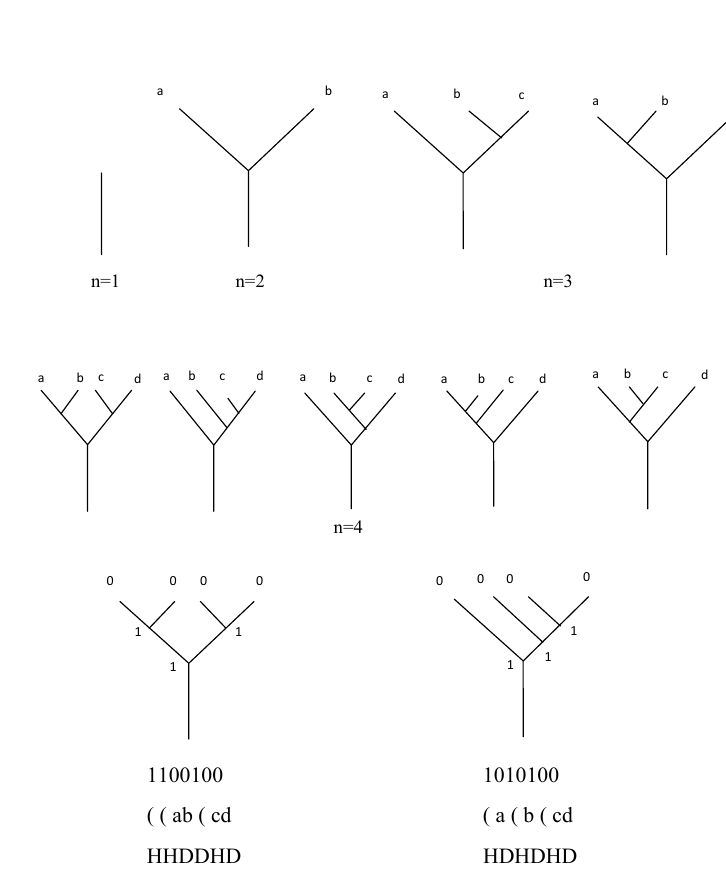
\includegraphics[width=1\linewidth]{../images/tri-trees}
\caption{Trivalent, planted trees with \(n\) leaves.\label{trivalenttrees}}
\end{figure}
\begin{figure}
\centering
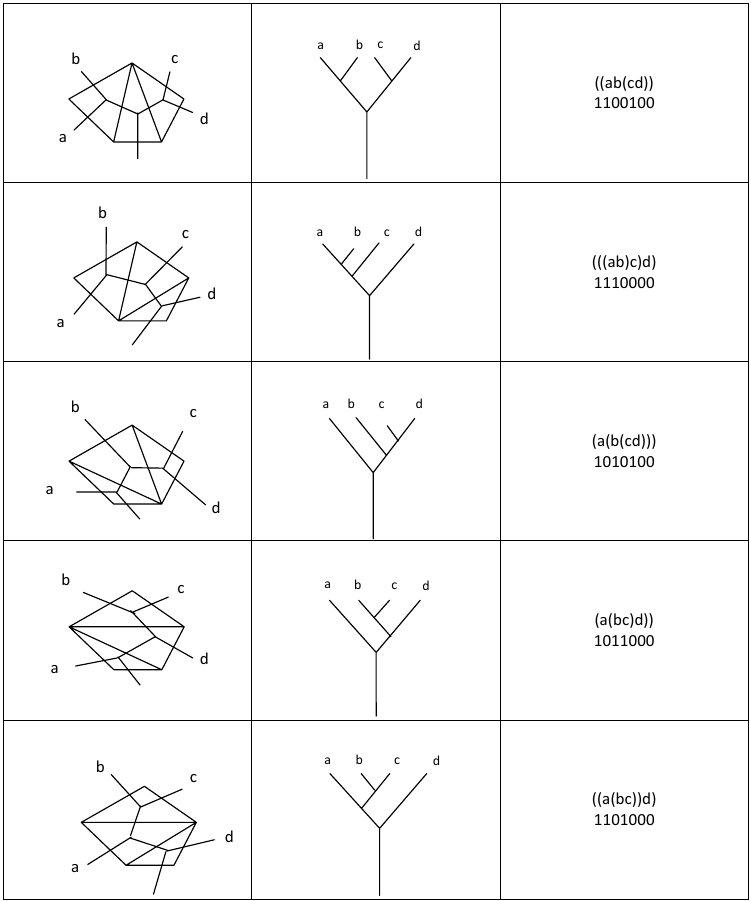
\includegraphics[width=1\linewidth]{../images/catalan-bijections.png}
\caption{\label{catalanbijections}}
\end{figure}
\typeout{************************************************}
\typeout{Exercises  Problems on Catalan Numbers}
\typeout{************************************************}
\subsection*{Problems on Catalan Numbers}\label{exercises-6}
\addcontentsline{toc}{subsection}{Problems on Catalan Numbers}
\begin{exerciselist}
\item[1.]\hypertarget{exercise-51}{}\hypertarget{p-618}{}%
Use the recursion for \(P_{n}\) and compute \(P_{6}\), and \(P_{7}\).%
\par\smallskip
\item[2.]\hypertarget{exercise-52}{}\hypertarget{p-619}{}%
Use the closed formula for \(P_n\) and compute \(P_{6}\) and \(P_{7}\).%
\par\smallskip
\item[3.]\hypertarget{exercise-53}{}\hypertarget{p-620}{}%
Use \(G = P_{1}x + P_{2}x^{2} +\cdots\) and the recursion for \(P_{n}\) to determine a closed formula for \(P_{n}\).%
\par\smallskip
\item[4.]\hypertarget{prob-workseq}{}\hypertarget{p-621}{}%
List the workable sequences for \(n = 4\).%
\par\smallskip
\item[5.]\hypertarget{prob-parenth}{}\hypertarget{p-622}{}%
List the \(P_{6}\) ways of parenthesizing \(abcdef\).%
\par\smallskip
\item[6.]\hypertarget{exercise-56}{}\hypertarget{p-623}{}%
Display a bijection between the 14 sequences in \hyperlink{prob-workseq}{Exercise~4} and the 14 products in \hyperlink{prob-parenth}{Exercise~5}.%
\par\smallskip
\item[7.]\hypertarget{exercise-57}{}\hypertarget{p-624}{}%
Find the nonworkable sequence associated with each: \leavevmode%
\begin{enumerate}[label=(\alph*)]
\item\hypertarget{li-111}{}\hypertarget{p-625}{}%
H H H D D H%
\item\hypertarget{li-112}{}\hypertarget{p-626}{}%
D H H H H D%
\item\hypertarget{li-113}{}\hypertarget{p-627}{}%
D D D H H H H H%
\item\hypertarget{li-114}{}\hypertarget{p-628}{}%
D D H H D H H H%
\end{enumerate}
%
\par\smallskip
\item[8.]\hypertarget{exercise-58}{}\hypertarget{p-629}{}%
Draw the \(T_{6}\) triangulations of a convex hexagon.%
\par\smallskip
\item[9.]\hypertarget{exercise-59}{}\hypertarget{p-630}{}%
Display a bijection between the 5 ways of parenthesizing \(abcd\) and the 5 triangulations of a convex pentagon.%
\par\smallskip
\item[10.]\hypertarget{exercise-60}{}\hypertarget{p-631}{}%
Let \(C_{n} = \frac{1}{n + 1}\binom{2n}{n}.\) Verifiy the formula:%
\begin{equation*}
C_{n} = \binom{n}{1} C_{n - 1} - \binom{n - 1}{2} C_{n - 2} + \binom{n - 2}{3} C_{n - 3} - \cdots
\end{equation*}
%
\par\smallskip
\item[11.]\hypertarget{exercise-61}{}\hypertarget{p-632}{}%
Verify that \(H_{3} = 5\) by drawing the required paths.%
\par\smallskip
\item[12.]\hypertarget{exercise-62}{}\hypertarget{p-633}{}%
Assign the appropriate binary sequences to each of the 5 trees for \(n=3\) in \hyperref[trivalenttrees]{Figure~\ref{trivalenttrees}}.%
\par\smallskip
\end{exerciselist}
\hypertarget{exercisegroup-1}{}\par\noindent \hypertarget{p-634}{}%
For each of the following, investigate bijections that relate one to another.%
\begin{exercisegroup}(1)
\exercise[13.]\hypertarget{exercise-63}{}\hypertarget{p-635}{}%
A and B each receive \(n\) votes. Let \(V_{n}\) denote the number of ways that the \(2n\) votes can be tallied so that A never trails B. Let \(V_{0} = 1\).%
\exercise[14.]\hypertarget{exercise-64}{}\hypertarget{p-636}{}%
Place \(2n\) points on the circumference of a circle and draw \(n\)  nonintersecting chords in \(D_{n}\) ways; \(D_{0} = 1\)%
\exercise[15.]\hypertarget{exercise-65}{}\hypertarget{p-637}{}%
In how many ways can \(1, 2, 3, \ldots, 2n\) be inserted into a \(2\times n\) rectangle such that the entries are increasing in rows and columns.  Let the answer be \(Y_n\); \(Y_1 = 1\), \(Y_2 = 2\).%
\exercise[16.]\hypertarget{exercise-66}{}\hypertarget{p-638}{}%
Place \(2n\) points on a line segment and join them in pairs by nonintersecting arcs above the segment. In how many ways can this be done? Call the answer \(S_{n}\); \(S_{1}=1\), \(S_{2}=2\).%
\exercise[17.]\hypertarget{exercise-67}{}\hypertarget{p-639}{}%
A rook on an \(n + 1\) by \(n + 1\) chessboard must move from the lower left corner to the upper right corner never going above the diagonal. How many paths are possible? Let \(K_{n}\) be the answer.%
\exercise[18.]\hypertarget{exercise-68}{}\hypertarget{p-640}{}%
On an \(n + 1\) by \(n + 1\) chessboard a king starts on the first row and moves one square forward or back along a fixed column and ends on the starting square after \(2n\) moves. In how many ways, \(G_{n}\) , can this be done?%
\exercise[19.]\hypertarget{exercise-69}{}\hypertarget{p-641}{}%
Count the number of planar rhyme schemes for a stanza consisting of \(n\) lines. Joanne Growney showed in her doctoral thesis that the Bell numbers, which count all rhyme schemes, have the Catalan numbers as a subsequence and that these enumerate precisely the planar rhyme schemes. For example, of the \(B_4 = 15\) rhyme schemes, \(C_4 = 14\) are planar. The nonplanar one is given by \(abab\).%
\end{exercisegroup}
\par\smallskip\noindent
\typeout{************************************************}
\typeout{Chapter 3 Advanced Combinatorics}
\typeout{************************************************}
\chapter[{Advanced Combinatorics}]{Advanced Combinatorics}\label{ch_sequences}
\hypertarget{p-642}{}%
ADD INTRODUCTION ABOUT SOME HARDER PROBLEMS THAT REQUIRE MORE ADVANCED TECHNIQUES%
\typeout{************************************************}
\typeout{Section 3.1 Advanced Counting Using PIE}
\typeout{************************************************}
\section[{Advanced Counting Using PIE}]{Advanced Counting Using PIE}\label{sec_advPIE}
\begin{investigation}[]\label{investigation-7}
\hypertarget{p-643}{}%
You have 11 identical mini key-lime pies to give to 4 children. However, you don't want any kid to get more than 3 pies. How many ways can you distribute the pies? %
\begin{enumerate}
\item\hypertarget{li-115}{}\hypertarget{p-644}{}%
How many ways are there to distribute the pies without any restriction?%
\item\hypertarget{li-116}{}\hypertarget{p-645}{}%
Let's get rid of the ways that one or more kid gets too many pies. How many ways are there to distribute the pies if Al gets too many pies? What if Bruce gets too many? Or Cat? Or Dent?%
\item\hypertarget{li-117}{}\hypertarget{p-646}{}%
What if two kids get too many pies? How many ways can this happen? Does it matter which two kids you pick to overfeed?%
\item\hypertarget{li-118}{}\hypertarget{p-647}{}%
Is it possible that three kids get too many pies? If so, how many ways can this happen?%
\item\hypertarget{li-119}{}\hypertarget{p-648}{}%
How should you combine all the numbers you found above to answer the original question?%
\end{enumerate}
%
\par
\hypertarget{p-649}{}%
Suppose now you have 13 pies and 7 children. No child can have more than 2 pies. How many ways can you distribute the pies?%
\end{investigation}
\hypertarget{p-650}{}%
Stars and bars allows us to count the number of ways to distribute 10 cookies to 3 kids and natural number solutions to \(x+y+z = 11\), for example. A relatively easy modification allows us to put a \emph{lower bound} restriction on these problems: perhaps each kid must get at least two cookies or \(x,y,z \ge 2\). This was done by first assigning each kid (or variable) 2 cookies (or units) and then distributing the rest using stars and bars.%
\par
\hypertarget{p-651}{}%
What if we wanted an \emph{upper bound} restriction? For example, we might insist that no kid gets more than 4 cookies or that \(x, y, z \le 4\). It turns out this is considerably harder, but still possible. The idea is to count all the distributions and then remove those that violate the condition. In other words, we must count the number of ways to distribute 11 cookies to 3 kids in which \emph{one or more} of the kids gets more than 4 cookies. For any particular kid, this is not a problem; we do this using stars and bars. But how to combine the number of ways for kid A, or B or C? We must use the PIE.%
\par
\hypertarget{p-652}{}%
The Principle of Inclusion/Exclusion (PIE) gives a method for finding the cardinality of the union of not necessarily disjoint sets. We saw in {$\langle\langle$Unresolved xref, reference "subsec\_PIE"; check spelling or use "provisional" attribute$\rangle\rangle$}\hyperlink{}{~} how this works with three sets. To find how many things are in \emph{one or more} of the sets \(A\), \(B\), and \(C\), we should just add up the number of things in each of these sets. However, if there is any overlap among the sets, those elements are counted multiple times. So we subtract the things in each intersection of a pair of sets. But doing this removes elements which are in all three sets once too often, so we need to add it back in. In terms of cardinality of sets, we have%
\begin{equation*}
|A \cup B \cup C| = |A| + |B| + |C| - |A \cap B| - |A \cap C| - |B \cap C| + |A\cap B \cap C|.
\end{equation*}
%
\begin{example}[]\label{example-11}
\hypertarget{p-653}{}%
Three kids, Alberto, Bernadette, and Carlos, decide to share 11 cookies. They wonder how many ways they could split the cookies up provided that none of them receive more than 4 cookies (someone receiving no cookies is for some reason acceptable to these kids).%
\par\smallskip%
\noindent\textbf{Solution.}\hypertarget{solution-54}{}\quad%
\hypertarget{p-654}{}%
Without the ``no more than 4'' restriction, the answer would be \({13 \choose 2}\), using 11 stars and 2 bars (separating the three kids). Now count the number of ways that one or more of the kids violates the condition, i.e., gets at least 4 cookies.%
\par
\hypertarget{p-655}{}%
Let \(A\) be the set of outcomes in which Alberto gets more than 4 cookies. Let \(B\) be the set of outcomes in which Bernadette gets more than 4 cookies. Let \(C\) be the set of outcomes in which Carlos gets more than 4 cookies. We then are looking (for the sake of subtraction) for the size of the set \(A \cup B \cup C\). Using PIE, we must find the sizes of \(|A|\), \(|B|\), \(|C|\), \(|A\cap B|\) and so on. Here is what we find.%
\par
\hypertarget{p-656}{}%
\leavevmode%
\begin{itemize}[label=\textbullet]
\item{}\(|A| = {8 \choose 2}\). First give Alberto 5 cookies, then distribute the remaining 6 to the three kids without restrictions, using 6 stars and 2 bars.%
\item{}\(|B| = {8 \choose 2}\). Just like above, only now Bernadette gets 5 cookies at the start.%
\item{}\(|C| = {8 \choose 2}\). Carlos gets 5 cookies first.%
\item{}\(|A \cap B| = {3 \choose 2}\). Give Alberto and Bernadette 5 cookies each, leaving 1 (star) to distribute to the three kids (2 bars).%
\item{}\(|A \cap C| = {3 \choose 2}\). Alberto and Carlos get 5 cookies first.%
\item{}\(|B \cap C| = {3 \choose 2}\). Bernadette and Carlos get 5 cookies first.%
\item{}\(|A \cap B \cap C| = 0\). It is not possible for all three kids to get 4 or more cookies.%
\end{itemize}
%
\par
\hypertarget{p-657}{}%
Combining all of these we see%
\begin{equation*}
|A \cup B \cup C| = {8 \choose 2} + {8 \choose 2} + {8 \choose 2} - {3 \choose 2} - {3 \choose 2} - {3 \choose 2} + 0 = 75.
\end{equation*}
%
\par
\hypertarget{p-658}{}%
Thus the answer to the original question is \({13 \choose 2} - 75 = 78 - 75 = 3\). This makes sense now that we see it. The only way to ensure that no kid gets more than 4 cookies is to give two kids 4 cookies and one kid 3; there are three choices for which kid that should be. We could have found the answer much quicker through this observation, but the point of the example is to illustrate that PIE works!%
\end{example}
\hypertarget{p-659}{}%
For four or more sets, we do not write down a formula for PIE. Instead, we just think of the principle: add up all the elements in single sets, then subtract out things you counted twice (elements in the intersection of a \emph{pair} of sets), then add back in elements you removed too often (elements in the intersection of groups of three sets), then take back out elements you added back in too often (elements in the intersection of groups of four sets), then add back in, take back out, add back in, etc. This would be very difficult if it wasn't for the fact that in these problems, all the cardinalities of the single sets are equal, as are all the cardinalities of the intersections of two sets, and that of three sets, and so on. Thus we can group all of these together and multiply by how many different combinations of 1, 2, 3, \textellipsis{} sets there are.%
\begin{example}[]\label{example-12}
\hypertarget{p-660}{}%
How many ways can you distribute 10 cookies to 4 kids so that no kid gets more than 2 cookies?%
\par\smallskip%
\noindent\textbf{Solution.}\hypertarget{solution-55}{}\quad%
\hypertarget{p-661}{}%
There are \({13 \choose 3}\) ways to distribute 10 cookies to 4 kids (using 10 stars and 3 bars).  We will subtract all the outcomes in which a kid gets 3 or more cookies. How many outcomes are there like that? We can force kid A to eat 3 or more cookies by giving him 3 cookies before we start. Doing so reduces the problem to one in which we have 7 cookies to give to 4 kids without any restrictions. In that case, we have 7 stars (the 7 remaining cookies) and 3 bars (one less than the number of kids) so we can distribute the cookies in \({10 \choose 3}\) ways. Of course we could choose any one of the 4 kids to give too many cookies, so it would appear that there are \({4 \choose 1}{10 \choose 3}\) ways to distribute the cookies giving too many to one kid. But in fact, we have over counted.%
\par
\hypertarget{p-662}{}%
We must get rid of the outcomes in which two kids have too many cookies. There are \({4 \choose 2}\) ways to select 2 kids to give extra cookies. It takes 6 cookies to do this, leaving only 4 cookies. So we have 4 stars and still 3 bars. The remaining 4 cookies can thus be distributed in \({7 \choose 3}\) ways (for each of the \({4 \choose 2}\) choices of which 2 kids to over-feed).%
\par
\hypertarget{p-663}{}%
But now we have removed too much. We must add back in all the ways to give too many cookies to three kids. This uses 9 cookies, leaving only 1 to distribute to the 4 kids using stars and bars, which can be done in \({4 \choose 3}\) ways. We must consider this outcome for every possible choice of which three kids we over-feed, and there are \({4 \choose 3}\) ways of selecting that set of 3 kids.%
\par
\hypertarget{p-664}{}%
Next we would subtract all the ways to give four kids too many cookies, but in this case, that number is 0.%
\par
\hypertarget{p-665}{}%
All together we get that the number of ways to distribute 10 cookies to 4 kids without giving any kid more than 2 cookies is:%
\begin{equation*}
{13 \choose 3} - \left[{4 \choose 1}{10 \choose 3} - {4 \choose 2}{7 \choose 3} + {4\choose 3}{4\choose 3}\right]
\end{equation*}
which is%
\begin{equation*}
286 - [480 - 210 + 16] = 0.
\end{equation*}
%
\par
\hypertarget{p-666}{}%
This makes sense: there is NO way to distribute 10 cookies to 4 kids and make sure that nobody gets more than 2. It is slightly surprising that%
\begin{equation*}
{13 \choose 3} = \left[{4 \choose 1}{10 \choose 3} - {4 \choose 2}{7 \choose 3} + {4\choose 3}{4\choose 3}\right]
\end{equation*}
but since PIE works, this equality must hold.%
\end{example}
\hypertarget{p-667}{}%
Just so you don't think that these problems always have easier solutions, consider the following example.%
\begin{example}[]\label{example-13}
\hypertarget{p-668}{}%
Earlier ({$\langle\langle$Unresolved xref, reference "example-stars-bars-int-sol"; check spelling or use "provisional" attribute$\rangle\rangle$}\hyperlink{}{~}) we counted the number of solutions to the equation%
\begin{equation*}
x_1 + x_2 + x_3 + x_4 + x_5 = 13
\end{equation*}
where \(x_i \ge 0\) for each \(x_i\).%
\par
\hypertarget{p-669}{}%
How many of those solutions have \(0 \le x_i \le 3\) for each \(x_i\)?%
\par\smallskip%
\noindent\textbf{Solution.}\hypertarget{solution-56}{}\quad%
\hypertarget{p-670}{}%
We must subtract off the number of solutions in which one or more of the variables has a value greater than 3. We will need to use PIE because counting the number of solutions for which each of the five variables separately are greater than 3 counts solutions multiple times. Here is what we get:%
\par
\hypertarget{p-671}{}%
\leavevmode%
\begin{itemize}[label=\textbullet]
\item{}\hypertarget{p-672}{}%
Total solutions: \({17 \choose 4}\).%
\item{}\hypertarget{p-673}{}%
Solutions where \(x_1 > 3\): \({13 \choose 4}\). Give \(x_1\) 4 units first, then distribute the remaining 9 units to the 5 variables.%
\item{}\hypertarget{p-674}{}%
Solutions where \(x_1 > 3\) and \(x_2 > 3\): \({9 \choose 4}\). After you give 4 units to \(x_1\) and another 4 to \(x_2\), you only have 5 units left to distribute.%
\item{}\hypertarget{p-675}{}%
Solutions where \(x_1 > 3\), \(x_2 > 3\) and \(x_3 > 3\): \({5 \choose 4}\).%
\item{}\hypertarget{p-676}{}%
Solutions where \(x_1 > 3\), \(x_2 > 3\), \(x_3 > 3\), and \(x_4 > 3\): 0.%
\end{itemize}
%
\par
\hypertarget{p-677}{}%
We also need to account for the fact that we could choose any of the five variables in the place of \(x_1\) above (so there will be \({5 \choose 1}\) outcomes like this), any pair of variables in the place of \(x_1\) and \(x_2\) (\({5 \choose 2}\) outcomes) and so on. It is because of this that the double counting occurs, so we need to use PIE. All together we have that the number of solutions with \(0 \le x_i \le 3\) is%
\begin{equation*}
{17 \choose 4} - \left[{5\choose 1}{13 \choose 4} - {5 \choose 2}{9 \choose 4} + {5 \choose 3}{5 \choose 4}\right] = 15.
\end{equation*}
%
\end{example}
\typeout{************************************************}
\typeout{Subsection  Counting Derangements}
\typeout{************************************************}
\subsection[{Counting Derangements}]{Counting Derangements}\label{subsec_derangements}
\begin{investigation}[]\label{investigation-8}
\hypertarget{p-678}{}%
For your senior prank, you decide to switch the nameplates on your favorite 5 professors' doors. So that none of them feel left out, you want to make sure that all of the nameplates end up on the wrong door. How many ways can this be accomplished?%
\end{investigation}
\hypertarget{p-679}{}%
The advanced use of PIE has applications beyond stars and bars. A \terminology{derangement}\index{derangement} of \(n\) elements \(\{1,2,3,\ldots, n\}\) is a permutation in which no element is fixed. For example, there are \(6\) permutations of the three elements \(\{1,2,3\}\):%
\begin{equation*}
123 ~~ 132 ~~ 213 ~~ 231 ~~ 312 ~~ 321.
\end{equation*}
but most of these have one or more elements fixed: \(123\) has all three elements fixed since all three elements are in their original positions, \(132\) has the first element fixed (1 is in its original first position), and so on. In fact, the only derangements of three elements are%
\begin{equation*}
231 \text{ and } 312.
\end{equation*}
%
\par
\hypertarget{p-680}{}%
If we go up to 4 elements, there are 24 permutations (because we have 4 choices for the first element, 3 choices for the second, 2 choices for the third leaving only 1 choice for the last). How many of these are derangements? If you list out all 24 permutations and eliminate those which are not derangements, you will be left with just 9 derangements. Let's see how we can get that number using PIE.%
\begin{example}[]\label{example-14}
\hypertarget{p-681}{}%
How many derangements are there of 4 elements?%
\par\smallskip%
\noindent\textbf{Solution.}\hypertarget{solution-57}{}\quad%
\hypertarget{p-682}{}%
We count all permutations, and subtract those which are not derangements. There are \(4! = 24\) permutations of 4 elements. Now for a permutation to \emph{not} be a derangement, at least one of the 4 elements must be fixed. There are \({4 \choose 1}\) choices for which single element we fix. Once fixed, we need to find a permutation of the other three elements. There are \(3!\) permutations on 3 elements. But now we have counted too many non-derangements, so we must subtract those permutations which fix two elements. There are \({4 \choose 2}\) choices for which two elements we fix, and then for each pair, \(2!\) permutations of the remaining elements. But this subtracts too many, so add back in permutations which fix 3 elements, all \({4 \choose 3}1!\) of them. Finally subtract the \({4 \choose 4}0!\) permutations (recall \(0! = 1\)) which fix all four elements. All together we get that the number of derangements of 4 elements is:%
\begin{equation*}
4! - \left[{4 \choose 1}3! - {4 \choose 2}2! + {4 \choose 3} 1! - {4 \choose 4}0!\right] = 24 - 15 = 9.
\end{equation*}
%
\end{example}
\hypertarget{p-683}{}%
Of course we can use a similar formula to count the derangements of any number of elements. However, the more elements we have, the longer the formula gets. Here is another example:%
\begin{example}[]\label{example-15}
\hypertarget{p-684}{}%
Five gentlemen attend a party, leaving their hats at the door. At the end of the party, they hastily grab hats on their way out. How many different ways could this happen so that none of the gentlemen leave with their own hat?%
\par\smallskip%
\noindent\textbf{Solution.}\hypertarget{solution-58}{}\quad%
\hypertarget{p-685}{}%
We are counting derangements on 5 elements. There are \(5!\) ways for the gentlemen to grab hats in any order\textemdash{}but many of these permutations will result in someone getting their own hat. So we subtract all the ways in which one or more of the men get their own hat. In other words, we subtract the non-derangements. Doing so requires PIE. Thus the answer is:%
\begin{equation*}
5! - \left[{5 \choose 1}4! - {5 \choose 2}3! + {5 \choose 3}2! - {5 \choose 4}1! + {5 \choose 5}0!\right].
\end{equation*}
%
\end{example}
\typeout{************************************************}
\typeout{Subsection  Counting Functions}
\typeout{************************************************}
\subsection[{Counting Functions}]{Counting Functions}\label{subsection-16}
\begin{investigation}[]\label{investigation-9}
\hypertarget{p-686}{}%
%
\begin{itemize}[label=\textbullet]
\item{}\hypertarget{p-687}{}%
Consider all functions \(f: \{1,2,3,4,5\} \to \{1,2,3,4,5\}\). How many functions are there all together? How many of those are injective? Remember, a function is an injection if every input goes to a different output.%
\item{}\hypertarget{p-688}{}%
Consider all functions \(f: \{1,2,3,4,5\} \to \{1,2,3,4,5\}\). How many of the \emph{injections} have the property that \(f(x) \ne x\) for any \(x \in \{1,2,3,4,5\}\)?%
\par
\hypertarget{p-689}{}%
Your friend claims that the answer is:%
\begin{equation*}
5! - \left[ {5\choose 1}4! - {5 \choose 2}3! + {5\choose 3}2! - {5 \choose 4}1! + {5\choose 5}0! \right].
\end{equation*}
%
\par
\hypertarget{p-690}{}%
Explain why this is correct.%
\item{}\hypertarget{p-691}{}%
Recall that a \emph{surjection} is a function for which every element of the codomain is in the range. How many of the functions \(f: \{1,2,3,4,5\} \to \{1,2,3,4,5\}\) are surjective? Use PIE!%
\end{itemize}
%
\end{investigation}
\hypertarget{p-692}{}%
We have seen throughout this chapter that many counting questions can be rephrased as questions about counting functions with certain properties.  This is reasonable since many counting questions can be thought of as counting the number of ways to assign elements from one set to elements of another.%
\begin{example}[]\label{example-16}
\hypertarget{p-693}{}%
You decide to give away your video game collection so to better spend your time studying advance mathematics. How many ways can you do this, provided: \leavevmode%
\begin{enumerate}
\item\hypertarget{li-135}{}You want to distribute your 3 different PS4 games among 5 friends, so that no friend gets more than one game?%
\item\hypertarget{li-136}{}You want to distribute your 8 different 3DS games among 5 friends?%
\item\hypertarget{li-137}{}You want to distribute your 8 different SNES games among 5 friends, so that each friend gets at least one game?%
\end{enumerate}
 In each case, model the counting question as a function counting question.%
\par\smallskip%
\noindent\textbf{Solution.}\hypertarget{solution-59}{}\quad%
\hypertarget{p-694}{}%
\leavevmode%
\begin{enumerate}
\item\hypertarget{li-138}{}\hypertarget{p-695}{}%
We must use the three games (call them 1, 2, 3) as the domain and the 5 friends (a,b,c,d,e) as the codomain (otherwise the function would not be defined for the whole domain when a friend didn't get any game).  So how many functions are there with domain \(\{1,2,3\}\) and codomain \(\{a,b,c,d,e\}\)?  The answer to this is \(5^3=125\), since we can assign any of 5 elements to be the image of 1, any of 5 elements to be the image of 2 and any of 5 elements to be the image of 3.%
\par
\hypertarget{p-696}{}%
But this is not the correct answer to our counting problem, because one of these functions is \(f= \twoline{1\amp 2\amp 3}{a\amp a\amp a}\); one friend can get more than one game.  What we really need to do is count \emph{injective} functions.  This gives \(P(5,3) = 60\) functions, which is the answer to our counting question.%
\item\hypertarget{li-139}{}\hypertarget{p-697}{}%
Again, we need to use the 8 games as the domain and the 5 friends as the codomain.  We are counting all functions, so the number of ways to distribute the games is \(5^8\).%
\item\hypertarget{li-140}{}\hypertarget{p-698}{}%
This question is harder.  Use the games as the domain and friends as the codomain (otherwise an element of the domain would have more than one image, which is impossible).  To ensure that every friend gets at least one game means that every element of the codomain is in the range.  In other words, we are looking for \emph{surjective} functions. How do you count those??%
\end{enumerate}
%
\end{example}
\hypertarget{p-699}{}%
In {$\langle\langle$Unresolved xref, reference "example-counting-functions-all"; check spelling or use "provisional" attribute$\rangle\rangle$}\hyperlink{}{~} we saw how to count all functions (using the multiplicative principle) and in {$\langle\langle$Unresolved xref, reference "example-counting-functions-injective"; check spelling or use "provisional" attribute$\rangle\rangle$}\hyperlink{}{~} we learned how to count injective functions (using permutations).  Surjective functions are not as easily counted (unless the size of the domain is smaller than the codomain, in which case there are none).%
\par
\hypertarget{p-700}{}%
The idea is to count the functions which are \emph{not} surjective, and then subtract that from the total number of functions. This works very well when the codomain has two elements in it:%
\begin{example}[]\label{example-17}
\hypertarget{p-701}{}%
How many functions \(f: \{1,2,3,4,5\} \to \{a,b\}\) are surjective?%
\par\smallskip%
\noindent\textbf{Solution.}\hypertarget{solution-60}{}\quad%
\hypertarget{p-702}{}%
There are \(2^5\) functions all together, two choices for where to send each of the 5 elements of the domain. Now of these, the functions which are \emph{not} surjective must exclude one or more elements of the codomain from the range. So first, consider functions for which \(a\) is not in the range. This can only happen one way: everything gets sent to \(b\). Alternatively, we could exclude \(b\) from the range. Then everything gets sent to \(a\), so there is only one function like this. These are the only ways in which a function could not be surjective (no function excludes both \(a\) and \(b\) from the range) so there are exactly \(2^5 - 2\) surjective functions.%
\end{example}
\hypertarget{p-703}{}%
When there are three elements in the codomain, there are now three choices for a single element to exclude from the range. Additionally, we could pick pairs of two elements to exclude from the range, and we must make sure we don't over count these. It's PIE time!%
\begin{example}[]\label{example-18}
\hypertarget{p-704}{}%
How many functions \(f: \{1,2,3,4,5\} \to \{a,b,c\}\) are surjective?%
\par\smallskip%
\noindent\textbf{Solution.}\hypertarget{solution-61}{}\quad%
\hypertarget{p-705}{}%
Again start with the total number of functions: \(3^5\) (as each of the five elements of the domain can go to any of three elements of the codomain). Now we count the functions which are \emph{not} surjective.%
\par
\hypertarget{p-706}{}%
Start by excluding \(a\) from the range. Then we have two choices (\(b\) or \(c\)) for where to send each of the five elements of the domain. Thus there are \(2^5\) functions which exclude \(a\) from the range. Similarly, there are \(2^5\) functions which exclude \(b\), and another \(2^5\) which exclude \(c\). Now have we counted all functions which are not surjective? Yes, but in fact, we have counted some multiple times. For example, the function which sends everything to \(c\) was one of the \(2^5\) functions we counted when we excluded \(a\) from the range, and also one of the \(2^5\) functions we counted when we excluded \(b\) from the range. We must subtract out all the functions which specifically exclude two elements from the range. There is 1 function when we exclude \(a\) and \(b\) (everything goes to \(c\)), one function when we exclude \(a\) and \(c\), and one function when we exclude \(b\) and \(c\).%
\par
\hypertarget{p-707}{}%
We are using PIE: to count the functions which are not surjective, we added up the functions which exclude \(a\), \(b\), and \(c\) separately, then subtracted the functions which exclude pairs of elements. We would then add back in the functions which exclude groups of three elements, except that there are no such functions. We find that the number of functions which are \emph{not} surjective is%
\begin{equation*}
2^5 + 2^5 + 2^5 - 1 - 1 - 1 + 0.
\end{equation*}
%
\par
\hypertarget{p-708}{}%
Perhaps a more descriptive way to write this is%
\begin{equation*}
{3 \choose 1}2^5 - {3 \choose 2}1^5 + {3 \choose 3}0^5.
\end{equation*}
since each of the \(2^5\)'s was the result of choosing 1 of the 3 elements of the codomain to exclude from the range, each of the three \(1^5\)'s was the result of choosing 2 of the 3 elements of the codomain to exclude. Writing \(1^5\) instead of 1 makes sense too: we have 1 choice of were to send each of the 5 elements of the domain.%
\par
\hypertarget{p-709}{}%
Now we can finally count the number of surjective functions:%
\begin{equation*}
3^5 - \left[{3 \choose 1}2^5 - {3 \choose 2}1^5\right] = 150.
\end{equation*}
%
\end{example}
\hypertarget{p-710}{}%
You might worry that to count surjective functions when the codomain is larger than 3 elements would be too tedious. We need to use PIE but with more than 3 sets the formula for PIE is very long. However, we have lucked out. As we saw in the example above, the number of functions which exclude a single element from the range is the same no matter which single element is excluded. Similarly, the number of functions which exclude a pair of elements will be the same for every pair. With larger codomains, we will see the same behavior with groups of 3, 4, and more elements excluded. So instead of adding/subtracting each of these, we can simply add or subtract all of them at once, if you know how many there are. This works just like it did in for the other types of counting questions in this section, only now the size of the various combinations of sets is a number raised to a power, as opposed to a binomial coefficient or factorial. Here's what happens with \(4\) and \(5\) elements in the codomain.%
\begin{example}[]\label{example-19}
\hypertarget{p-711}{}%
\leavevmode%
\begin{enumerate}
\item\hypertarget{li-141}{}\hypertarget{p-712}{}%
How many functions \(f: \{1,2,3,4,5\} \to \{a,b,c,d\}\) are surjective?%
\item\hypertarget{li-142}{}\hypertarget{p-713}{}%
How many functions \(f: \{1,2,3,4,5\} \to \{a,b,c,d,e\}\) are surjective?%
\end{enumerate}
%
\par\smallskip%
\noindent\textbf{Solution.}\hypertarget{solution-62}{}\quad%
\hypertarget{p-714}{}%
\leavevmode%
\begin{enumerate}
\item\hypertarget{li-143}{}\hypertarget{p-715}{}%
There are \(4^5\) functions all together; we will subtract the functions which are not surjective.  We could exclude any one of the four elements of the codomain, and doing so will leave us with \(3^5\) functions for each excluded element.  This counts too many so we subtract the functions which exclude two of the four elements of the codomain, each pair giving \(2^5\) functions.  But this excludes too many, so we add back in the functions which exclude three of the four elements of the codomain, each triple giving \(1^5\) function.  There are \({4 \choose 1}\) groups of functions excluding a single element, \({4 \choose 2}\) groups of functions excluding a pair of elements, and \({4 \choose 3}\) groups of functions excluding a triple of elements.  This means that the number of functions which are \emph{not} surjective is:%
\begin{equation*}
{4 \choose 1}3^5 - {4 \choose 2}2^5 + {4 \choose 3}1^5.
\end{equation*}
We can now say that the number of functions which are surjective is:%
\begin{equation*}
4^5 - \left[{4 \choose 1}3^5 - {4 \choose 2}2^5 + {4 \choose 3}1^5\right].
\end{equation*}
%
\item\hypertarget{li-144}{}\hypertarget{p-716}{}%
The number of surjective functions is:%
\begin{equation*}
5^5 - \left[{5 \choose 1}4^5 - {5 \choose 2}3^5 + {5 \choose 3}2^5 - {5 \choose 4}1^5\right].
\end{equation*}
We took the total number of functions \(5^5\) and subtracted all that were not surjective.  There were \({5 \choose 1}\) ways to select a single element from the codomain to exclude from the range, and for each there were \(4^5\) functions.  But this double counts, so we use PIE and subtract functions excluding two elements from the range: there are \({5 \choose 2}\) choices for the two elements to exclude, and for each pair, \(3^5\) functions.  This takes out too many functions, so we add back in functions which exclude 3 elements from the range: \({5 \choose 3}\) choices for which three to exclude, and then \(2^5\) functions for each choice of elements.  Finally we take back out the 1 function which excludes 4 elements for each of the \({5 \choose 4}\) choices of 4 elements.%
\par
\hypertarget{p-717}{}%
If you happen to calculate this number precisely, you will get 120 surjections.  That happens to also be the value of \(5!\).  This might seem like an amazing coincidence until you realize that every surjective function \(f:X \to Y\) with \(\card{X} = \card{Y}\) finite must necessarily be a bijection.  The number of bijections is always \(\card{X}!\) in this case.  What we have here is a \emph{combinatorial proof} of the following identity:%
\begin{equation*}
n^n - \left[{n\choose 1}(n-1)^n - {n \choose 2}(n-2)^n + \cdots + {n \choose n-1}1^n \right] = n!.
\end{equation*}
%
\end{enumerate}
%
\end{example}
\hypertarget{p-718}{}%
We have seen that counting surjective functions is another nice example of the advanced use of the Principle of Inclusion/Exclusion. Also, counting injective functions turns out to be equivalent to permutations, and counting all functions has a solution akin to those counting problems where order matters but repeats are allowed (like counting the number of words you can make from a given set of letters).%
\par
\hypertarget{p-719}{}%
These are not just a few more examples of the techniques we have developed in this chapter. Quite the opposite: everything we have learned in this chapter are examples of \emph{counting functions}!%
\begin{example}[]\label{example-20}
\hypertarget{p-720}{}%
How many 5-letter words can you make using the eight letters \(a\) through \(h\)? How many contain no repeated letters?%
\par\smallskip%
\noindent\textbf{Solution.}\hypertarget{solution-63}{}\quad%
\hypertarget{p-721}{}%
By now it should be no surprise that there are \(8^5\) words, and \(P(8,5)\) words without repeated letters. The new piece here is that we are actually counting functions. For the first problem, we are counting all functions from \(\{1,2,\ldots, 5\}\) to \(\{a,b,\ldots, h\}\). The numbers in the domain represent the \emph{position} of the letter in the word, the codomain represents the letter that could be assigned to that position. If we ask for no repeated letters, we are asking for injective functions.%
\par
\hypertarget{p-722}{}%
If \(A\) and \(B\) are \emph{any} sets with \(|A| = 5\) and \(|B| = 8\), then the number of functions \(f: A \to B\) is \(8^5\) and the number of injections is \(P(8,5)\). So if you can represent your counting problem as a function counting problem, most of the work is done.%
\end{example}
\begin{example}[]\label{example-21}
\hypertarget{p-723}{}%
How many subsets are there of \(\{1,2,\ldots, 9\}\)? How many 9-bit strings are there (of any weight)?%
\par\smallskip%
\noindent\textbf{Solution.}\hypertarget{solution-64}{}\quad%
\hypertarget{p-724}{}%
We saw in \hyperref[sec_counting-binom]{Section~\ref{sec_counting-binom}} that the answer to both these questions is \(2^9\), as we can say yes or no (or 0 or 1) to each of the 9 elements in the set (positions in the bit-string). But \(2^9\) also looks like the answer you get from counting functions. In fact, if you count all functions \(f: A \to B\) with \(|A| = 9\) and \(|B| = 2\), this is exactly what you get.%
\par
\hypertarget{p-725}{}%
This makes sense! Let \(A = \{1,2,\ldots, 9\}\) and \(B = \{y, n\}\). We are assigning each element of the set either a yes or a no. Or in the language of bit-strings, we would take the 9 positions in the bit string as our domain and the set \(\{0,1\}\) as the codomain.%
\end{example}
\hypertarget{p-726}{}%
So far we have not used a function as a model for binomial coefficients (combinations). Think for a moment about the relationship between combinations and permutations, say specifically \({9 \choose 3}\) and \(P(9,3)\). We \emph{do} have a function model for \(P(9,3)\). This is the number of \emph{injective} functions from a set of size 3 (say \(\{1,2,3\}\) to a set of size 9 (say \(\{1,2,\ldots, 9\}\)) since there are 9 choices for where to send the first element of the domain, then only 8 choices for the second, and 7 choices for the third. For example, the function might look like this:%
\begin{equation*}
f(1) = 5 \qquad f(2) = 8 \qquad f(3) = 4.
\end{equation*}
%
\par
\hypertarget{p-727}{}%
This is a different function from:%
\begin{equation*}
f(1) = 4 \qquad f(2) = 5 \qquad f(3) = 8.
\end{equation*}
%
\par
\hypertarget{p-728}{}%
Now \(P(9,3)\) counts these as different outcomes correctly, but \({9\choose 3}\) will count these (among others) as just one outcome. In fact, in terms of functions \({9 \choose 3}\) just counts the number of different ranges possible of injective functions. This should not be a surprise since binomial coefficients counts subsets, and the range is a possible subset of the codomain.\footnote{A more mathematically sophisticated interpretation of combinations is that we are defining two injective functions to be \emph{equivalent} if they have the same range, and then counting the number of equivalence classes under this notion of equivalence.\label{fn-5}}%
\par
\hypertarget{p-729}{}%
While it is possible to interpret combinations as functions, perhaps the better advice is to instead use combinations (or stars and bars) when functions are not quite the right way to interpret the counting question.%
\typeout{************************************************}
\typeout{Subsection  Chromatic Polynomials (again)}
\typeout{************************************************}
\subsection[{Chromatic Polynomials (again)}]{Chromatic Polynomials (again)}\label{subsection-17}
\typeout{************************************************}
\typeout{Exercises  Exercises}
\typeout{************************************************}
\subsection*{Exercises}\label{exercises_counting-advPIE}
\addcontentsline{toc}{subsection}{Exercises}
\begin{exerciselist}
\item[1.]\hypertarget{exercise-70}{}\hypertarget{p-730}{}%
The dollar menu at your favorite tax-free fast food restaurant has 7 items. You have \textdollar{}10 to spend. How many different meals can you buy if you spend all your money and: \leavevmode%
\begin{enumerate}[label=(\alph*)]
\item\hypertarget{li-145}{}\hypertarget{p-731}{}%
Purchase at least one of each item.%
\item\hypertarget{li-146}{}\hypertarget{p-732}{}%
Possibly skip some items.%
\item\hypertarget{li-147}{}\hypertarget{p-733}{}%
Don't get more than 2 of any particular item.%
\end{enumerate}
%
\par\smallskip
\item[2.]\hypertarget{exercise-71}{}\hypertarget{p-735}{}%
After a late night of math studying, you and your friends decide to go to your favorite tax-free fast food Mexican restaurant, \emph{Burrito Chime}. You decide to order off of the dollar menu, which has 7 items. Your group has \textdollar{}16 to spend (and will spend all of it). \leavevmode%
\begin{enumerate}[label=(\alph*)]
\item\hypertarget{li-151}{}\hypertarget{p-736}{}%
How many different orders are possible? Explain. (The \emph{order} in which the order is placed does not matter - just which and how many of each item that is ordered.) %
\item\hypertarget{li-152}{}\hypertarget{p-737}{}%
How many different orders are possible if you want to get at least one of each item? Explain. %
\item\hypertarget{li-153}{}\hypertarget{p-738}{}%
How many different orders are possible if you don't get more than 4 of any one item? Explain. %
\end{enumerate}
%
\par\smallskip
\item[3.]\hypertarget{exercise-72}{}\hypertarget{p-739}{}%
After another gym class you are tasked with putting the 14 identical dodgeballs away into 5 bins. This time, no bin can hold more than 6 balls. How many ways can you clean up?%
\par\smallskip
\item[4.]\hypertarget{exercise-73}{}\hypertarget{p-741}{}%
Consider the equation \(x_1 + x_2 + x_3 + x_4 = 15\). How many solutions are there with \(2 \le x_i \le 5\) for all \(i \in \{1,2,3,4\}\)?%
\par\smallskip
\item[5.]\hypertarget{exercise-74}{}\hypertarget{p-745}{}%
Suppose you planned on giving 7 gold stars to some of the 13 star students in your class. Each student can receive at most one star. How many ways can you do this? Use PIE, and also an easier method, and compare your results.%
\par\smallskip
\item[6.]\hypertarget{exercise-75}{}\hypertarget{p-746}{}%
Based on the previous question, give a combinatorial proof for the identity:%
\begin{equation*}
{n \choose k} = {n+k-1 \choose k} - \sum_{j=1}^n (-1)^{j+1}{n \choose j}{n+k-(2j+1) \choose k}.
\end{equation*}
%
\par\smallskip
\item[7.]\hypertarget{exercise-76}{}\hypertarget{p-747}{}%
Illustrate how the counting of derangements works by writing all permutations of \(\{1,2,3,4\}\) and the crossing out those which are not derangements. Keep track of the permutations you cross out more than once, using PIE.%
\par\smallskip
\item[8.]\hypertarget{exercise-77}{}\hypertarget{p-749}{}%
How many permutations of \(\{1,2,3,4,5\}\) leave exactly 1 element fixed?%
\par\smallskip
\item[9.]\hypertarget{exercise-78}{}\hypertarget{p-751}{}%
Ten ladies of a certain age drop off their red hats at the hat check of a museum. As they are leaving, the hat check attendant gives the hats back randomly. In how many ways can exactly six of the ladies receive their own hat (and the other four not)?  Explain.%
\par\smallskip
\item[10.]\hypertarget{exercise-79}{}\hypertarget{p-752}{}%
The Grinch sneaks into a room with 6 Christmas presents to 6 different people. He proceeds to switch the name-labels on the presents. How many ways could he do this if: \leavevmode%
\begin{enumerate}[label=(\alph*)]
\item\hypertarget{li-154}{}\hypertarget{p-753}{}%
No present is allowed to end up with its original label? Explain what each term in your answer represents. %
\item\hypertarget{li-155}{}\hypertarget{p-754}{}%
Exactly 2 presents keep their original labels? Explain. %
\item\hypertarget{li-156}{}\hypertarget{p-755}{}%
Exactly 5 presents keep their original labels? Explain. %
\end{enumerate}
%
\par\smallskip
\item[11.]\hypertarget{exercise-80}{}\hypertarget{p-756}{}%
Consider functions \(f: \{1,2,3,4\} \to \{a,b,c,d,e,f\}\). How many functions have the property that \(f(1) \ne a\) or \(f(2) \ne b\), or both?%
\par\smallskip
\item[12.]\hypertarget{exercise-81}{}\hypertarget{p-758}{}%
Consider sets \(A\) and \(B\) with \(|A| = 10\) and \(|B| = 5\). How many functions \(f: A \to B\) are surjective?%
\par\smallskip
\item[13.]\hypertarget{exercise-82}{}\hypertarget{p-760}{}%
Let \(A = \{1,2,3,4,5\}\). How many injective functions \(f:A \to A\) have the property that for each \(x \in A\), \(f(x) \ne x\)?%
\par\smallskip
\item[14.]\hypertarget{exercise-83}{}\hypertarget{p-761}{}%
Let \(d_n\) be the number of derangements of \(n\) objects. For example, using the techniques of this section, we find%
\begin{equation*}
d_3 = 3!-\left({3 \choose 1}2! - {3 \choose 2}1! + {3 \choose 3}0! \right)
\end{equation*}
We can use the formula for \({n \choose k}\) to write this all in terms of factorials.  After simplifying, for \(d_3\) we would get%
\begin{equation*}
d_3 = 3!\left(1 - \frac{1}{1} + \frac{1}{2} - \frac{1}{6} \right)
\end{equation*}
Generalize this to find a nicer formula for \(d_n\).  Bonus: For large \(n\), approximately what fraction of all permutations are derangements?  Use your knowledge of Taylor series from calculus.%
\par\smallskip
\end{exerciselist}
\typeout{************************************************}
\typeout{Section 3.2 Generating Functions}
\typeout{************************************************}
\section[{Generating Functions}]{Generating Functions}\label{section-12}
\hypertarget{p-762}{}%
ADD MATERIAL FROM BOGART ON COUNTING WITH GENERATING FUNCTIONS. Maybe this should be moved to be with the sequences stuff, and then sprinkled back through the other stuff.  Whenever we do it, we can put examples from previous topics here, or put questions for future topics related to generating functions there.%
\par
\hypertarget{p-763}{}%
There is an extremely powerful tool in discrete mathematics used to manipulate sequences called the generating function. The idea is this: instead of an infinite sequence (for example: \(2, 3, 5, 8, 12, \ldots\)) we look at a single function which encodes the sequence. But not a function which gives the \(n\)th term as output. Instead, a function whose power series (like from calculus) ``displays'' the terms of the sequence. So for example, we would look at the power series \(2 + 3x + 5x^2 + 8x^3 + 12x^4 + \cdots\) which displays the sequence \(2, 3, 5, 8, 12, \ldots\) as coefficients.%
\par
\hypertarget{p-764}{}%
An infinite power series is simply an infinite sum of terms of the form \(c_nx^n\) were \(c_n\) is some constant. So we might write a power series like this:%
\begin{equation*}
\sum_{k=0}^\infty c_k x^k.
\end{equation*}
or expanded like this%
\begin{equation*}
c_0 + c_1x + c_2x^2 + c_3x^3 + c_4x^4 + c_5x^5 + \cdots.
\end{equation*}
%
\par
\hypertarget{p-765}{}%
When viewed in the context of generating functions, we call such a power series a \emph{generating series}. The generating series generates the sequence%
\begin{equation*}
c_0, c_1, c_2, c_3, c_4, c_5, \ldots.
\end{equation*}
%
\par
\hypertarget{p-766}{}%
In other words, the sequence generated by a generating series is simply the sequence of \emph{coefficients} of the infinite polynomial.%
\begin{example}[]\label{example-22}
\hypertarget{p-767}{}%
What sequence is represented by the generating series \(3 + 8x^2 + x^3 + \frac{x^5}{7} + 100x^6 + \cdots\)?%
\par\smallskip%
\noindent\textbf{Solution.}\hypertarget{solution-72}{}\quad%
\hypertarget{p-768}{}%
We just read off the coefficients of each \(x^n\) term. So \(a_0 = 3\) since the coefficient of \(x^0\) is 3 (\(x^0 = 1\) so this is the constant term). What is \(a_1\)? It is NOT 8, since 8 is the coefficient of \(x^2\), so 8 is the term \(a_2\) of the sequence. To find \(a_1\) we need to look for the coefficient of \(x^1\) which in this case is 0. So \(a_1 = 0\). Continuing, we have \(a_2 = 8\), \(a_3 = 1\), \(a_4 = 0\), and \(a_5 = \frac{1}{7}\). So we have the sequence%
\begin{equation*}
3, 0, 8, 1, \frac{1}{7}, 100, \ldots
\end{equation*}
%
\par
\hypertarget{p-769}{}%
Note that when discussing generating functions, we always start our sequence with \(a_0\).%
\end{example}
\hypertarget{p-770}{}%
Now you might very naturally ask why we would do such a thing. One reason is that encoding a sequence with a power series helps us keep track of which term is which in the sequence. For example, if we write the sequence \(1, 3, 4, 6, 9, \ldots, 24, 41,\ldots\) it is impossible to determine which term \(24\) is (even if we agreed that the first term was supposed to be \(a_0\)). However, if we wrote the generating series instead, we would have \(1 + 3x + 4x^2 + 6x^3 + 9x^4 + \cdots + 24 x^{17} + 41 x^{18} + \cdots\). Now it is clear that 24 is the 17th term of the sequence (that is, \(a_{17} = 24\)). Of course to get this benefit we could have displayed our sequence in any number of ways, perhaps \(\fbox{1}_0 \fbox{3}_1 \fbox{4}_2 \fbox{6}_3 \fbox{9}_4 \cdots \fbox{24}_{17}\fbox{41}_{18}\cdots\), but we do not do this. The reason is that the generating series looks like an ordinary power series (although we are interpreting it differently) so we can do things with it that we ordinarily do with power series such as write down what it converges to.%
\par
\hypertarget{p-771}{}%
For example, from calculus we know that the power series \(1 + x + \frac{x^2}{2} + \frac{x^3}{6} + \frac{x^4}{24} + \cdots + \frac{x^n}{n!} + \cdots\) converges to the function \(e^x\). So we can use \(e^x\) as a way of talking about the sequence of coefficients of the power series for \(e^x\). When we write down a nice compact function which has an infinite power series that we view as a generating series, then we call that function a \emph{generating function}. In this example, we would say%
\begin{equation*}
1, 1, \frac{1}{2}, \frac{1}{6}, \frac{1}{24}, \ldots, \frac{1}{n!}, \ldots \mbox{ has generating function }  e^x
\end{equation*}
%
\typeout{************************************************}
\typeout{Subsection  Building Generating Functions}
\typeout{************************************************}
\subsection[{Building Generating Functions}]{Building Generating Functions}\label{subsection-18}
\hypertarget{p-772}{}%
The \(e^x\) example is very specific. We have a rather odd sequence, and the only reason we know its generating function is because we happen to know the Taylor series for \(e^x\). Our goal now is to gather some tools to build the generating function of a particular given sequence.%
\par
\hypertarget{p-773}{}%
Let's see what the generating functions are for some very simple sequences. The simplest of all: 1, 1, 1, 1, 1, \textellipsis{}. What does the \emph{generating series} look like? It is simply \(1 + x + x^2 + x^3 + x^4 + \cdots\). Now, can we find a closed formula for this power series? Yes! This particular series is really just a geometric series with common ratio \(x\). So if we use our ``multiply, shift and subtract'' technique from {$\langle\langle$Unresolved xref, reference "sec\_seq-arithgeom"; check spelling or use "provisional" attribute$\rangle\rangle$}\hyperlink{}{~}, we have%
\begin{align*}
S \amp  = 1 + x + x^2 + x^3 + \cdots\\
\underline{- xS} \amp  \underline{\,\, = ~~~~~~ x + x^2 + x^3 + x^4 + \cdots}\\
(1-x)S \amp  = 1
\end{align*}
%
\par
\hypertarget{p-774}{}%
Therefore we see that%
\begin{equation*}
1 + x + x^2 + x^3 \cdots = \dfrac{1}{1-x}
\end{equation*}
%
\par
\hypertarget{p-775}{}%
You might remember from calculus that this is only true on the interval of convergence for the power series, in this case when \(|x| \lt  1\). That is true for us, but we don't care. We are never going to plug anything in for \(x\), so as long as there is some value of \(x\) for which the generating function and generating series agree, we are happy. And in this case we are happy.%
\begin{assemblage}[\(1,1,1,\ldots\)]\label{assemblage-10}
\hypertarget{p-776}{}%
The generating function for \(1,1,1,1,1,1,\ldots\) is \(\dfrac{1}{1-x}\)%
\end{assemblage}
\hypertarget{p-777}{}%
Let's use this basic generating function to find generating functions for more sequences. What if we replace \(x\) by \(-x\). We get%
\begin{equation*}
\frac{1}{1+x} = 1 - x + x^2 - x^3 + \cdots \mbox{ which generates }  1, -1, 1, -1, \ldots
\end{equation*}
%
\par
\hypertarget{p-778}{}%
If we replace \(x\) by \(3x\) we get%
\begin{equation*}
\frac{1}{1-3x} = 1 + 3x + 9x^2 + 27x^3 + \cdots \mbox{ which generates }  1, 3, 9, 27, \ldots
\end{equation*}
%
\par
\hypertarget{p-779}{}%
By replacing the \(x\) in \(\frac{1}{1-x}\) we can get generating functions for a variety of sequences, but not all. For example, you cannot plug in anything for \(x\) to get the generating function for \(2,2,2,2, \ldots\). However, we are not lost yet. Notice that each term of \(2, 2, 2, 2, \ldots\) is the result of multiplying the terms of \(1, 1, 1, 1, \ldots\) by the constant 2. So multiply the generating function by 2 as well.%
\begin{equation*}
\frac{2}{1-x} = 2 + 2x + 2x^2 + 2x^3 + \cdots \mbox{ which generates }  2, 2, 2, 2, \ldots
\end{equation*}
%
\par
\hypertarget{p-780}{}%
Similarly, to find the generating function for the sequence \(3, 9, 27, 81, \ldots\), we note that this sequence is the result of multiplying each term of \(1, 3, 9, 27, \ldots\) by 3. Since we have the generating function for \(1, 3, 9, 27, \ldots\) we can say%
\begin{equation*}
\frac{3}{1-3x} = 3\cdot 1 + 3\cdot 3x + 3\cdot 9x^2 + 3\cdot 27x^3 + \cdots \mbox{ which generates }  3, 9, 27, 81, \ldots
\end{equation*}
%
\par
\hypertarget{p-781}{}%
What about the sequence \(2, 4, 10, 28, 82, \ldots\)? Here the terms are always 1 more than powers of 3. That is, we have added the sequences \(1,1,1,1,\ldots\) and \(1,3,9, 27,\ldots\) term by term. Therefore we can get a generating function by adding the respective generating functions:%
\begin{align*}
2 + 4x + 10x^2 + 28x^3 + \cdots  \amp  = (1 + 1) + (1 + 3)x + (1 + 9)x^2 + (1 + 27)x^3 + \cdots\\
\amp  = 1 + x + x^2 + x^3 + \cdots + 1 + 3x + 9x^2 + 27x^3 + \cdots\\
\amp  = \frac{1}{1-x} + \frac{1}{1-3x}
\end{align*}
%
\par
\hypertarget{p-782}{}%
The fun does not stop there: if we replace \(x\) in our original generating function by \(x^2\) we get%
\begin{equation*}
\frac{1}{1-x^2} = 1 + x^2  + x^4 + x^6\cdots \mbox{ which generates }  1, 0, 1, 0, 1, 0, \ldots.
\end{equation*}
%
\par
\hypertarget{p-783}{}%
How could we get \(0,1,0,1,0,1,\ldots\)? Start with the previous sequence and \emph{shift} it over by 1. But how do you do this? To see how shifting works, let's first try to get the generating function for the sequence \(0, 1, 3, 9, 27, \ldots\). We know that \(\frac{1}{1-3x} = 1 + 3x + 9x^2 + 27x^3 + \cdots\). To get the zero out front, we need the generating series to look like \(x + 3x^2 + 9x^3 + 27x^4+ \cdots\) (so there is no constant term). Multiplying by \(x\) has this effect. So the generating function for \(0, 1, 3, 9, 27, \ldots\) is \(\frac{x}{1-3x}\). This will also work to get the generating function for \(0,1,0,1,0,1,\ldots\):%
\begin{equation*}
\frac{x}{1-x^2} = x + x^3 + x^5 + \cdots \mbox{ which generates }  0, 1, 0, 1, 0 , 1 \ldots
\end{equation*}
%
\par
\hypertarget{p-784}{}%
What if we add the sequences \(1,0,1,0,1,0,\ldots\) and \(0,1,0,1,0,1,\ldots\) term by term? We should get \(1,1,1,1,1,1\ldots\). What happens when we add the generating functions? It works (try it)!%
\begin{equation*}
\frac{1}{1-x^2} + \frac{x}{1-x^2} = \frac{1}{1-x}.
\end{equation*}
%
\par
\hypertarget{p-785}{}%
Here's a sneaky one: what happens if you take the \emph{derivative} of \(\frac{1}{1-x}\)? We get \(\frac{1}{(1-x)^2}\). On the other hand, if we differentiate term by term in the power series, we get \((1 + x + x^2 + x^3 + \cdots)' = 1 + 2x + 3x^2 + 4x^3 + \cdots\) which is the generating series for \(1, 2, 3, 4, \ldots\). This says%
\begin{assemblage}[\(1,2,3,\ldots\)]\label{assemblage-11}
\hypertarget{p-786}{}%
The generating function for \(1, 2, 3, 4, 5, \ldots\) is \(\d\frac{1}{(1-x)^2}.\)%
\end{assemblage}
\hypertarget{p-787}{}%
Take a second derivative: \(\frac{2}{(1-x)^3} = 2 + 6x + 12x^2 + 20x^3 + \cdots\). So \(\frac{1}{(1-x)^3} = 1 + 3x + 6x^2 + 10x^3 + \cdots\) is a generating function for the triangular numbers, \(1,3,6,10\ldots\) (although here we have \(a_0 = 1\) while \(T_0 = 0\) usually).%
\typeout{************************************************}
\typeout{Subsection  Differencing}
\typeout{************************************************}
\subsection[{Differencing}]{Differencing}\label{subsection-19}
\hypertarget{p-788}{}%
We have seen how to find generating functions from \(\frac{1}{1-x}\) using multiplication (by a constant or by \(x\)), substitution, addition, and differentiation. To use each of these, you must notice a way to transform the sequence \(1,1,1,1,1\ldots\) into your desired sequence. This is not always easy. It is also not really the way we have analyzed sequences. One thing we have considered often is the sequence of differences between terms of a sequence. This will turn out to be helpful in finding generating functions as well. The sequence of differences is often simpler than the original sequence. So if we know a generating function for the differences, we would like to use this to find a generating function for the original sequence.%
\par
\hypertarget{p-789}{}%
For example, consider the sequence \(2, 4, 10, 28, 82, \ldots\). How could we move to the sequence of first differences: \(2, 6, 18, 54,\ldots\)? We want to subtract 2 from the 4, 4 from the 10, 10 from the 28, and so on. So if we subtract (term by term) the sequence \(0, 2, 4, 10, 28,\ldots\) from \(2, 4, 10, 28\ldots\), we will be set. We can get the generating function for \(0,2,4,10,28,\ldots\) from the generating function for \(2,4,10,28\ldots\) by multiplying by \(x\). Use \(A\) to represent the generating function for \(2, 4, 10, 28, 82, \ldots\) Then:%
\begin{align*}
A \amp  = 2 + 4x + 10x^2 +28x^3 + 82x^4 + \cdots\\
\underline{-xA} \amp  \underline{\,\,= 0 + 2x + 4x^2 + 10x^3 + 28 x^4 + 82x^5 + \cdots}\\
(1-x)A \amp  = 2 + 2x + 6x^2 + 18x^3 + 54x^4 + \cdots
\end{align*}
%
\par
\hypertarget{p-790}{}%
While we don't get exactly the sequence of differences, we do get something close. In this particular case, we already know the generating function \(A\) (we found it in the previous section) but most of the time we will use this differencing technique to \emph{find} \(A\): if we have the generating function for the sequence of differences, we can then solve for \(A\).%
\begin{example}[]\label{example-23}
\hypertarget{p-791}{}%
Find a generating function for \(1, 3, 5, 7, 9,\ldots\).%
\par\smallskip%
\noindent\textbf{Solution.}\hypertarget{solution-73}{}\quad%
\hypertarget{p-792}{}%
Notice that the sequence of differences is constant. We know how to find the generating function for any constant sequence. So denote the generating function for \(1, 3, 5, 7, 9, \ldots\) by \(A\). We have%
\begin{align*}
A \amp  = 1 + 3x + 5x^2 + 7x^3 + 9x^4 + \cdots\\
\underline{-xA} \amp  \underline{\,\,= 0 + x + 3x^2 +  5x^3 + 7x^4 + 9x^5 + \cdots}\\
(1-x)A \amp  = 1 + 2x + 2x^2 + 2x^3 + 2x^4 + \cdots
\end{align*}
%
\par
\hypertarget{p-793}{}%
We know that \(2x + 2x^2 + 2x^3 + 2x^4 + \cdots = \dfrac{2x}{1-x}\). Thus%
\begin{equation*}
(1-x)A = 1 + \frac{2x}{1-x}.
\end{equation*}
%
\par
\hypertarget{p-794}{}%
Now solve for \(A\):%
\begin{equation*}
A = \frac{1}{1-x} + \frac{2x}{(1-x)^2} = \frac{1+x}{(1-x)^2}.
\end{equation*}
%
\par
\hypertarget{p-795}{}%
Does this makes sense? Before we simplified the two fractions into one, we were adding the generating function for the sequence \(1,1,1,1,\ldots\) to the generating function for the sequence \(0, 2, 4, 6, 8, 10, \ldots\) (remember \(\frac{1}{(1-x)^2}\) generates \(1,2,3,4,5, \ldots\), multiplying by \(2x\) shifts it over, putting the zero out front, and doubles each term). If we add these term by term, we get the correct sequence \(1,3,5,7, 9, \ldots\).%
\end{example}
\hypertarget{p-796}{}%
Now that we have a generating function for the odd numbers, we can use that to find the generating function for the squares:%
\begin{example}[]\label{example-24}
\hypertarget{p-797}{}%
Find the generating function for \(1, 4, 9, 16, \ldots\). Note we take \(1 = a_0\).%
\par\smallskip%
\noindent\textbf{Solution.}\hypertarget{solution-74}{}\quad%
\hypertarget{p-798}{}%
Again we call the generating function for the sequence \(A\). Using differencing:%
\begin{align*}
A \amp  = 1 + 4x + 9x^2 + 16x^3 + \cdots\\
\underline{- xA} \amp  \underline{\,\, = 0 + x + 4x^2 + 9x^3 + 16x^4 + \cdots}\\
(1-x)A \amp  = 1 + 3x + 5x^2 + 7x^3 + \cdots
\end{align*}
%
\par
\hypertarget{p-799}{}%
Since \(1 + 3x + 5x^2 + 7x^3 + \cdots = \d\frac{1+x}{(1-x)^2}\) we have \(A = \d\frac{1+x}{(1-x)^3}\).%
\end{example}
\hypertarget{p-800}{}%
In each of the examples above, we found the difference between consecutive terms which gave us a sequence of differences for which we knew a generating function. We can generalize this to more complicated relationships between terms of the sequence. For example, if we know that the sequence satisfies the recurrence relation \(a_n = 3a_{n-1} - 2a_{n-2}\)? In other words, if we take a term of the sequence and subtract 3 times the previous term and then add 2 times the term before that, we get 0 (since \(a_n - 3a_{n-1} + 2a_{n-2} = 0\)). That will hold for all but the first two terms of the sequence. So after the first two terms, the sequence of results of these calculations would be a sequence of 0's, for which we definitely know a generating function.%
\begin{example}[]\label{example-25}
\hypertarget{p-801}{}%
The sequence \(1, 3, 7, 15, 31, 63, \ldots\) satisfies the recurrence relation \(a_n = 3a_{n-1} - 2a_{n-2}\). Find the generating function for the sequence.%
\par\smallskip%
\noindent\textbf{Solution.}\hypertarget{solution-75}{}\quad%
\hypertarget{p-802}{}%
Call the generating function for the sequence \(A\). We have%
\begin{align*}
A \amp  = 1 + 3x + 7x^2 + 15x^3 + 31x^4 + \cdots + a_nx^n + \cdots\\
-3xA \amp  = 0 - 3x - 9x^2 - 21x^3 - 45x^4 - \cdots - 3a_{n-1}x^n - \cdots\\
\underline{+~~~2x^2A_{~}^{~^{~}}} \amp  \underline{\,\, = 0 + 0x + 2x^2 + 6x^3 + 14x^4 + \cdots + 2a_{n-2}x^n + \cdots}\\
(1-3x+2x^2)A \amp  = 1
\end{align*}
%
\par
\hypertarget{p-803}{}%
We multiplied \(A\) by \(-3x\) which shifts every term over one spot and multiplies them by \(-3\). On the third line, we multiplied \(A\) by \(2x^2\), which shifted every term over two spots and multiplied them by 2. When we add up the corresponding terms, we are taking each term, subtracting 3 times the previous term, and adding 2 times the term before that. This will happen for each term after \(a_1\) because \(a_n - 3a_{n-1} + 2a_{n-2} = 0\). In general, we might have two terms from the beginning of the generating series, although in this case the second term happens to be 0 as well.%
\par
\hypertarget{p-804}{}%
Now we just need to solve for \(A\):%
\begin{equation*}
A = \frac{1}{1 - 3x + 2x^2}.
\end{equation*}
%
\end{example}
\typeout{************************************************}
\typeout{Subsection  Multiplication and Partial Sums}
\typeout{************************************************}
\subsection[{Multiplication and Partial Sums}]{Multiplication and Partial Sums}\label{subsection-20}
\hypertarget{p-805}{}%
What happens to the sequences when you multiply two generating functions? Let's see: \(A = a_0 + a_1x + a_2x^2 + \cdots\) and \(B = b_0 + b_1x + b_2x^2 + \cdots\). To multiply \(A\) and \(B\), we need to do a lot of distributing (infinite FOIL?) but keep in mind we will group like terms and only need to write down the first few terms to see the pattern. The constant term is \(a_0b_0\). The coefficient of \(x\) is \(a_0b_1 + a_1b_0\). And so on. We get:%
\begin{equation*}
AB = a_0b_0 + (a_0b_1 + a_1b_0)x + (a_0b_2 + a_1b_1 + a_2b_0)x^2 + (a_0b_3 + a_1b_2 + a_2b_1 + a_3b_0)x^3 + \cdots
\end{equation*}
%
\begin{example}[]\label{example-26}
\hypertarget{p-806}{}%
``Multiply'' the sequence \(1, 2, 3, 4, \ldots\) by the sequence \(1, 2, 4, 8, 16, \ldots\).%
\par\smallskip%
\noindent\textbf{Solution.}\hypertarget{solution-76}{}\quad%
\hypertarget{p-807}{}%
The new constant term is just \(1 \cdot 1\). The next term will be \(1\cdot 2 + 2 \cdot 1 = 4\). The next term: \(1 \cdot 4 + 2 \cdot 2 + 3 \cdot 1 = 11\). One more: \(1 \cdot 8 + 2 \cdot 4 + 3 \cdot 2 + 4 \cdot 1 = 28\). The resulting sequence is%
\begin{equation*}
1, 4, 11, 28, 57, \ldots
\end{equation*}
%
\par
\hypertarget{p-808}{}%
Since the generating function for \(1,2,3,4, \ldots\) is \(\frac{1}{(1-x)^2}\) and the generating function for \(1,2,4,8, 16, \ldots\) is \(\frac{1}{1-2x}\), we have that the generating function for \(1,4, 11, 28, 57, \ldots\) is \(\frac{1}{(1-x)^2(1-2x)}\)%
\end{example}
\hypertarget{p-809}{}%
Consider the special case when you multiply a sequence by \(1, 1, 1, \ldots\). For example, multiply \(1,1,1,\ldots\) by \(1, 2, 3, 4, 5\ldots\). The first term is \(1\cdot 1 = 1\). Then \(1\cdot 2 + 1 \cdot 1 = 3\). Then \(1\cdot 3 + 1\cdot 2 + 1 \cdot 1 = 6\). The next term will be 10. We are getting the triangular numbers. More precisely, we get the sequence of partial sums of \(1,2,3,4,5, \ldots\). In terms of generating functions, we take \(\frac{1}{1-x}\) (generating \(1,1,1,1,1\ldots\)) and multiply it by \(\frac{1}{(1-x)^2}\) (generating \(1,2,3,4,5,\ldots\)) and this give \(\frac{1}{(1-x)^3}\). This should not be a surprise as we found the same generating function for the triangular numbers earlier.%
\par
\hypertarget{p-810}{}%
The point is, if you need to find a generating function for the sum of the first \(n\) terms of a particular sequence, and you know the generating function for \emph{that} sequence, you can multiply it by  \(\frac{1}{1-x}\). To go back from the sequence of partial sums to the original sequence, you look at the sequence of differences. When you get the sequence of differences you end up multiplying by \(1-x\), or equivalently, dividing by \(\frac{1}{1-x}\). Multiplying by \(\frac{1}{1-x}\) gives partial sums, dividing by \(\frac{1}{1-x}\) gives differences.%
\typeout{************************************************}
\typeout{Subsection  Solving Recurrence Relations with Generating Functions}
\typeout{************************************************}
\subsection[{Solving Recurrence Relations with Generating Functions}]{Solving Recurrence Relations with Generating Functions}\label{subsection-21}
\hypertarget{p-811}{}%
We conclude with an example of one of the many reasons studying generating functions is helpful. We can use generating functions to solve recurrence relations.%
\begin{example}[]\label{example-27}
\hypertarget{p-812}{}%
Solve the recurrence relation \(a_n = 3a_{n-1} - 2a_{n-2}\) with initial conditions \(a_0 = 1\) and \(a_1 = 3\).%
\par\smallskip%
\noindent\textbf{Solution.}\hypertarget{solution-77}{}\quad%
\hypertarget{p-813}{}%
We saw in an example above that this recurrence relation gives the sequence \(1, 3, 7, 15, 31, 63, \ldots\) which has generating function \(\dfrac{1}{1 - 3x + 2x^2}\). We did this by calling the generating function \(A\) and then computing \(A - 3xA + 2x^2A\) which was just 1, since every other term canceled out.%
\par
\hypertarget{p-814}{}%
But how does knowing the generating function help us? First, break up the generating function into two simpler ones. For this, we can use partial fraction decomposition. Start by factoring the denominator:%
\begin{equation*}
\frac{1}{1-3x + 2x^2} = \frac{1}{(1-x)(1-2x)}.
\end{equation*}
%
\par
\hypertarget{p-815}{}%
Partial fraction decomposition tells us that we can write this faction as the sum of two fractions (we decompose the given fraction):%
\begin{equation*}
\frac{1}{(1-x)(1-2x)} = \frac{a}{1-x} + \frac{b}{1-2x} \text{ ~~ for some constants } a \text{ and } b.
\end{equation*}
%
\par
\hypertarget{p-816}{}%
To find \(a\) and \(b\) we add the two decomposed fractions using a common denominator. This gives%
\begin{equation*}
\frac{1}{(1-x)(1-2x)} = \frac{a(1-2x) + b(1-x)}{(1-x)(1-2x)}.
\end{equation*}
so%
\begin{equation*}
1 = a(1-2x) + b(1-x).
\end{equation*}
%
\par
\hypertarget{p-817}{}%
This must be true for all values of \(x\). If \(x = 1\), then the equation becomes \(1 = -a\) so \(a = -1\). When \(x = \frac{1}{2}\) we get \(1 = b/2\) so \(b = 2\). This tells us that we can decompose the fraction like this:%
\begin{equation*}
\frac{1}{(1-x)(1-2x)} = \frac{-1}{1-x} + \frac{2}{1-2x}.
\end{equation*}
%
\par
\hypertarget{p-818}{}%
This completes the partial fraction decomposition. Notice that these two fractions are generating functions we know. In fact, we should be able to expand each of them.%
\begin{equation*}
\frac{-1}{1-x} = -1 - x - x^2 -x^3 - x^4 - \cdots \mbox{ which generates }  -1, -1, -1, -1, -1, \ldots.
\end{equation*}
%
\begin{equation*}
\frac{2}{1-2x} = 2 + 4x + 8x^2 + 16x^3 + 32x^4 + \cdots \mbox{ which generates }  2, 4, 8, 16, 32, \ldots.
\end{equation*}
%
\par
\hypertarget{p-819}{}%
We can give a closed formula for the \(n\)th term of each of these sequences. The first is just \(a_n = -1\). The second is \(a_n = 2^{n+1}\). The sequence we are interested in is just the sum of these, so the solution to the recurrence relation is%
\begin{equation*}
a_n = 2^{n+1} - 1
\end{equation*}
%
\end{example}
\hypertarget{p-820}{}%
We can now add generating functions to our list of methods for solving recurrence relations.%
\typeout{************************************************}
\typeout{Exercises  Exercises}
\typeout{************************************************}
\subsection*{Exercises}\label{exercises-8}
\addcontentsline{toc}{subsection}{Exercises}
\begin{exerciselist}
\item[1.]\hypertarget{exercise-84}{}\hypertarget{p-821}{}%
Find the generating function for each of the following sequences by relating them back to a sequence with known generating function.%
\par
\hypertarget{p-822}{}%
\leavevmode%
\begin{enumerate}[label=(\alph*)]
\item\hypertarget{li-157}{}\(4,4,4,4,4,\ldots\).%
\item\hypertarget{li-158}{}\(2, 4, 6, 8, 10, \ldots\).%
\item\hypertarget{li-159}{}\(0,0,0,2,4,6,8,10,\ldots\).%
\item\hypertarget{li-160}{}\(1, 5, 25, 125, \ldots\).%
\item\hypertarget{li-161}{}\(1, -3, 9, -27, 81, \ldots\).%
\item\hypertarget{li-162}{}\(1, 0, 5, 0, 25, 0, 125, 0, \ldots\).%
\item\hypertarget{li-163}{}\(0, 1, 0, 0, 2, 0, 0, 3, 0, 0, 4, 0, 0, 5, \ldots\).%
\end{enumerate}
%
\par\smallskip
\item[2.]\hypertarget{exercise-85}{}\hypertarget{p-824}{}%
Find the sequence generated by the following generating functions:%
\par
\hypertarget{p-825}{}%
\leavevmode%
\begin{enumerate}[label=(\alph*)]
\item\hypertarget{li-171}{}\(\dfrac{4x}{1-x}\).%
\item\hypertarget{li-172}{}\(\dfrac{1}{1-4x}\).%
\item\hypertarget{li-173}{}\(\dfrac{x}{1+x}\).%
\item\hypertarget{li-174}{}\(\dfrac{3x}{(1+x)^2}\).%
\item\hypertarget{li-175}{}\(\dfrac{1+x+x^2}{(1-x)^2}\) (Hint: multiplication).%
\end{enumerate}
%
\par\smallskip
\item[3.]\hypertarget{exercise-86}{}\hypertarget{p-827}{}%
Show how you can get the generating function for the triangular numbers in three different ways:%
\par
\hypertarget{p-828}{}%
\leavevmode%
\begin{enumerate}[label=(\alph*)]
\item\hypertarget{li-181}{}\hypertarget{p-829}{}%
Take two derivatives of the generating function for \(1,1,1,1,1, \ldots\)%
\item\hypertarget{li-182}{}\hypertarget{p-830}{}%
Use differencing.%
\item\hypertarget{li-183}{}\hypertarget{p-831}{}%
Multiply two known generating functions.%
\end{enumerate}
%
\par\smallskip
\item[4.]\hypertarget{exercise-87}{}\hypertarget{p-836}{}%
Use differencing to find the generating function for \(4, 5, 7, 10, 14, 19, 25, \ldots\).%
\par\smallskip
\item[5.]\hypertarget{exercise-88}{}\hypertarget{p-838}{}%
Find a generating function for the sequence with recurrence relation \(a_n = 3a_{n-1} - a_{n-2}\) with initial terms \(a_0 = 1\) and \(a_1 = 5\).%
\par\smallskip
\item[6.]\hypertarget{exercise-89}{}\hypertarget{p-840}{}%
Use the recurrence relation for the Fibonacci numbers to find the generating function for the Fibonacci sequence.%
\par\smallskip
\item[7.]\hypertarget{exercise-90}{}\hypertarget{p-842}{}%
Use multiplication to find the generating function for the sequence of partial sums of Fibonacci numbers, \(S_0, S_1, S_2, \ldots\) where \(S_0 = F_0\), \(S_1 = F_0 + F_1\), \(S_2 = F_0 + F_1 + F_2\), \(S_3 = F_0 + F_1 + F_2 + F_3\) and so on.%
\par\smallskip
\item[8.]\hypertarget{exercise-91}{}\hypertarget{p-844}{}%
Find the generating function for the sequence with closed formula \(a_n = 2(5^n) + 7(-3)^n\).%
\par\smallskip
\item[9.]\hypertarget{exercise-92}{}\hypertarget{p-846}{}%
Find a closed formula for the \(n\)th term of the sequence with generating function \(\dfrac{3x}{1-4x} + \dfrac{1}{1-x}\).%
\par\smallskip
\item[10.]\hypertarget{exercise-93}{}\hypertarget{p-848}{}%
Find \(a_7\) for the sequence with generating function \(\dfrac{2}{(1-x)^2}\cdot\dfrac{x}{1-x-x^2}\).%
\par\smallskip
\item[11.]\hypertarget{exercise-94}{}\hypertarget{p-850}{}%
Explain how we know that \(\dfrac{1}{(1-x)^2}\) is the generating function for \(1, 2, 3, 4, \ldots\).%
\par\smallskip
\item[12.]\hypertarget{exercise-95}{}\hypertarget{p-852}{}%
Starting with the generating function for \(1,2,3,4, \ldots\), find a generating function for each of the following sequences.%
\par
\hypertarget{p-853}{}%
\leavevmode%
\begin{enumerate}[label=(\alph*)]
\item\hypertarget{li-187}{}\(1, 0, 2, 0, 3, 0, 4,\ldots\).%
\item\hypertarget{li-188}{}\(1, -2, 3, -4, 5, -6, \ldots\).%
\item\hypertarget{li-189}{}\(0, 3, 6, 9, 12, 15, 18, \ldots\).%
\item\hypertarget{li-190}{}\(0, 3, 9, 18, 30, 45, 63,\ldots\). (Hint: relate this sequence to the previous one.)%
\end{enumerate}
%
\par\smallskip
\item[13.]\hypertarget{exercise-96}{}\hypertarget{p-855}{}%
You may assume that \(1, 1, 2, 3, 5, 8,\ldots\) has generating function \(\dfrac{1}{1-x-x^2}\) (because it does). Use this fact to find the sequence generated by each of the following generating functions.%
\par
\hypertarget{p-856}{}%
\leavevmode%
\begin{enumerate}[label=(\alph*)]
\item\hypertarget{li-195}{}\(\frac{x^2}{1-x-x^2}\).%
\item\hypertarget{li-196}{}\(\frac{1}{1-x^2-x^4}\).%
\item\hypertarget{li-197}{}\(\frac{1}{1-3x-9x^2}\).%
\item\hypertarget{li-198}{}\(\frac{1}{(1-x-x^2)(1-x)}\).%
\end{enumerate}
%
\par\smallskip
\item[14.]\hypertarget{exercise-97}{}\hypertarget{p-858}{}%
Find the generating function for the sequence \(1, -2, 4, -8, 16, \ldots\).%
\par\smallskip
\item[15.]\hypertarget{exercise-98}{}\hypertarget{p-860}{}%
Find the generating function for the sequence \(1, 1, 1, 2, 3, 4, 5, 6, \ldots\).%
\par\smallskip
\item[16.]\hypertarget{exercise-99}{}\hypertarget{p-862}{}%
Suppose \(A\) is the generating function for the sequence \(3, 5, 9, 15, 23, 33, \ldots\).%
\par
\hypertarget{p-863}{}%
\leavevmode%
\begin{enumerate}[label=(\alph*)]
\item\hypertarget{li-203}{}\hypertarget{p-864}{}%
Find a generating function (in terms of \(A\)) for the sequence of differences between terms.%
\item\hypertarget{li-204}{}\hypertarget{p-865}{}%
Write the sequence of differences between terms and find a generating function for it (without referencing \(A\)).%
\item\hypertarget{li-205}{}\hypertarget{p-866}{}%
Use your answers to parts (a) and (b) to find the generating function for the original sequence.%
\end{enumerate}
%
\par\smallskip
\end{exerciselist}
\typeout{************************************************}
\typeout{Section 3.3 Sterling Numbers of the 2nd Kind}
\typeout{************************************************}
\section[{Sterling Numbers of the 2nd Kind}]{Sterling Numbers of the 2nd Kind}\label{sec_adv-stirling}
\begin{activity}[Worksheet on Stirling numbers of the 2nd kind]\label{activity-42}
\hypertarget{p-869}{}%
\emph{DEFINITION:} \(S\left( n,k \right)\) is the number of ways of partitioning an \(n\)-set into \(k\) nonempty subsets.%
\begin{enumerate}[font=\bfseries,label=(\alph*),ref=\alph*]
\item\label{task-58} \hypertarget{p-870}{}%
Compute \(S(3,1)\), \(S(4,1)\) and \(S(n,1)\).%
\item\label{task-59} \hypertarget{p-871}{}%
Compute \(S(2,2)\), \(S(3,2)\) and \(S(4,2)\) .%
\item\label{task-60} \hypertarget{p-872}{}%
Compute \(S(3,3)\), and \(S(4,3)\).%
\item\label{task-61} \hypertarget{p-873}{}%
Find formulas and give proofs for \(S(n,n)\), \(S(n,2)\) \(S(n,n - 1)\), and \(S(n,n-2)\).%
\item\label{task-62} \hypertarget{p-874}{}%
Determine a recursion for \(S(n,k)\) by examining the following: In computing \(S\left( 4,3 \right)\) look back at the two cases: \leavevmode%
\begin{enumerate}
\item\hypertarget{li-209}{}\hypertarget{p-875}{}%
``Social'': The element 4 is part of another set.%
\item\hypertarget{li-210}{}\hypertarget{p-876}{}%
``Antisocial'': The element 4 stands alone.%
\item\hypertarget{li-211}{}\hypertarget{p-877}{}%
Deduce a recursion \(S\left( n,k \right) =\)%
\end{enumerate}
%
\item\label{task-63} \hypertarget{p-878}{}%
Make the first 5 rows of the Stirling Triangle.%
\end{enumerate}
\end{activity}
\hypertarget{p-879}{}%
A distribution of 4 different (often we say distinguishable) objects \(1,2,3,4\) into 3 similar (often we say indistinguishable) boxes, each of which becomes non-empty is modeled by partitioning \(\{ 1,2,3,4\}\) into 3 nonempty subsets. The six ways of doing this are listed next:%
% group protects changes to lengths, releases boxes (?)
{% begin: group for a single side-by-side
% set panel max height to practical minimum, created in preamble
\setlength{\panelmax}{0pt}
\ifdefined\panelboxAtabular\else\newsavebox{\panelboxAtabular}\fi%
\savebox{\panelboxAtabular}{%
\raisebox{\depth}{\parbox{0.5\linewidth}{\centering\begin{tabular}{ll}
\(\{4\}, \{1\}, \{2,3\}\)&\(\{1,4\}, \{2\}, \{3\}\)\tabularnewline[0pt]
\(\{4\}, \{2\}, \{1,3\}\)&\(\{1\}, \{2,4\}, \{3\}\)\tabularnewline[0pt]
\(\{4\}, \{3\}, \{1,2\}\)&\(\{1\}, \{2\}, \{3,4\}\)
\end{tabular}
}}}
\ifdefined\phAtabular\else\newlength{\phAtabular}\fi%
\setlength{\phAtabular}{\ht\panelboxAtabular+\dp\panelboxAtabular}
\settototalheight{\phAtabular}{\usebox{\panelboxAtabular}}
\setlength{\panelmax}{\maxof{\panelmax}{\phAtabular}}
\leavevmode%
% begin: side-by-side as tabular
% \tabcolsep change local to group
\setlength{\tabcolsep}{0\linewidth}
% @{} suppress \tabcolsep at extremes, so margins behave as intended
\par\medskip\noindent
\hspace*{0.25\linewidth}%
\begin{tabular}{@{}*{1}{c}@{}}
\begin{minipage}[c][\panelmax][t]{0.5\linewidth}\usebox{\panelboxAtabular}\end{minipage}\end{tabular}\\
% end: side-by-side as tabular
}% end: group for a single side-by-side
\par
\hypertarget{p-880}{}%
The Stirling numbers of the second kind, denoted by \(S(n,k)\), give the number of ways of partitioning an \(n\)-set into \(k\) non-empty subsets. Here \(k \in \{1,2,\ldots\}\) and \(n \geq k\). The above example shows \(S(4, 3) = 6\). Also notice that there are two cases: 4 is alone, or 4 is in some other batch; we can conclude that \(S(4, 3) = 3S(3,3) + S(3,2)\) since if 4 is in a singleton set just partition the remaining 3 into 2 sets and otherwise 4 can join any of the 3 batches of 3 elements.%
\begin{theorem}[{}]\label{thm-stirling-recursion}
\hypertarget{p-881}{}%
\(S(n,k) = kS(n - 1,k) + S(n - 1,k - 1)\)%
\end{theorem}
\begin{proof}\hypertarget{proof-11}{}
\hypertarget{p-882}{}%
We partition \(\{1,2,\ldots,n\}\) into \(k\) non-empty subsets in \(S(n,k)\) ways. If \(n\) is in a singleton set, there are \(S(n - 1,k - 1)\) ways to partition the remaining \(n - 1\) elements into \(k - 1\) subsets. Otherwise, the element \(n\) can join any of the \(k\) batches of \(n-1\) elements in \(kS(n - 1,k)\) ways.%
\end{proof}
\hypertarget{p-883}{}%
Polya, in Notes on Introductory Combinatorics, refers to these as the ``antisocial'' and ``social'' cases.%
\par
\hypertarget{p-884}{}%
The reader should check that \(S(3,3) = 1\) and that \(S(3,2) = 3\) so that \(S(4,3) = 3 \cdot 1 + 3 = 6\).%
\typeout{************************************************}
\typeout{Paragraphs  Border Formulas}
\typeout{************************************************}
\paragraph[{Border Formulas}]{Border Formulas}\hypertarget{paragraphs-14}{}
\hypertarget{p-885}{}%
The reader should verify that \(S(n,1) = 1\) and \(S(n,n) = 1\) for \(n \in Z^{+}\). From these border formulas and the recursion in \hyperref[thm-stirling-recursion]{Theorem~\ref{thm-stirling-recursion}} the following Stirling's Second Triangle can be made.%
% group protects changes to lengths, releases boxes (?)
{% begin: group for a single side-by-side
% set panel max height to practical minimum, created in preamble
\setlength{\panelmax}{0pt}
\ifdefined\panelboxAtabular\else\newsavebox{\panelboxAtabular}\fi%
\savebox{\panelboxAtabular}{%
\raisebox{\depth}{\parbox{0.5\linewidth}{\centering\begin{tabular}{lllllllll}
&&&&1&&&&\tabularnewline[0pt]
&&&1&&1&&&\tabularnewline[0pt]
&&1&&3&&1&&\tabularnewline[0pt]
&1&&7&&7&&1&\tabularnewline[0pt]
1&&15&&25&&10&&1
\end{tabular}
}}}
\ifdefined\phAtabular\else\newlength{\phAtabular}\fi%
\setlength{\phAtabular}{\ht\panelboxAtabular+\dp\panelboxAtabular}
\settototalheight{\phAtabular}{\usebox{\panelboxAtabular}}
\setlength{\panelmax}{\maxof{\panelmax}{\phAtabular}}
\leavevmode%
% begin: side-by-side as tabular
% \tabcolsep change local to group
\setlength{\tabcolsep}{0\linewidth}
% @{} suppress \tabcolsep at extremes, so margins behave as intended
\par\medskip\noindent
\hspace*{0.25\linewidth}%
\begin{tabular}{@{}*{1}{c}@{}}
\begin{minipage}[c][\panelmax][t]{0.5\linewidth}\usebox{\panelboxAtabular}\end{minipage}\end{tabular}\\
% end: side-by-side as tabular
}% end: group for a single side-by-side
\begin{theorem}[{}]\label{thm-stirling-border}
\hypertarget{p-886}{}%
\leavevmode%
\begin{enumerate}
\item\hypertarget{li-212}{}\hypertarget{p-887}{}%
\(S\left( n,n - 1 \right) =\binom{n}{2}\)%
\item\hypertarget{li-213}{}\hypertarget{p-888}{}%
\(S\left( n,2 \right) = 2^{n - 1} - 1\)%
\item\hypertarget{li-214}{}\hypertarget{p-889}{}%
\(S\left( n,n - 2 \right) =\binom{n}{3}
+ 3\binom{n}{4}\)%
\item\hypertarget{li-215}{}\hypertarget{p-890}{}%
\(S\left( n,n - 3 \right) =\binom{n}{4}
+ 10\binom{n}{5}
+ 15\binom{n}{6}\)%
\end{enumerate}
%
\end{theorem}
\hypertarget{p-891}{}%
You are asked to prove these in the problems.%
\par
\hypertarget{p-892}{}%
The entries in the Pascal Triangle, \(\binom{n}{k}\), satisfy the nice recursion \(\binom{n}{k} = \binom{n - 1}{k} + \binom{n - 1}{k - 1}\) and also have a closed formula: \(\binom{n}{k} = \frac{n!}{k!(n - k)!}\). \hyperref[thm-stirling-recursion]{Theorem~\ref{thm-stirling-recursion}} gives us a recursion for the Stirling numbers \(S(n,k)\) and, unfortunately, the best we can do for a ``closed'' formula is contained in the following.%
\begin{theorem}[{}]\label{thm-stirling-closed}
\hypertarget{p-893}{}%
%
\begin{equation*}
S(n,k) = \frac{1}{k!}\left[k^{n} - \binom{k}{1} \left( k - 1 \right)^{n} + \binom{k}{2} \left( k - 2 \right)^{n} - \binom{k}{3} \left( k - 3 \right)^{n} + \ldots + \left( - 1 \right)^{k - 1}\binom{k}{k - 1} 1^{n} \right] 
\end{equation*}
%
\end{theorem}
\begin{proof}\hypertarget{proof-12}{}
\hypertarget{p-894}{}%
The following argument is due to Polya. Suppose you wished to paint n houses and you have \(k\) different colors available. The first house can be painted in \(k\) different ways, the second in \(k\) different ways, etc. So there are \(k^{n}\) ways. How many ways actually use all \(k\) colors? Let \(\alpha_{i}\) be the property that no house is painted with the \(i\)th color, and let \(N(\alpha_{i})\) denote the number of ways of painting the \(n\) houses without using the \(i\)th color. Analogously for \(N(\alpha_{i},\alpha_{j})\), \(N(\alpha_{i},\alpha_{j},\alpha_{k})\), etc. Since \(N(\alpha_{i}) = (k - 1)^{n}\), \(N(a_{i},\alpha_{j}) = ( k - 2)^{n}\) and so on, the number of ways of painting \(n\) houses using all \(k\) colors is, using PIE, \(k^{n} -\binom{k}{1} \left(k - 1 \right)^{n} + \binom{k}{2} \left( k - 2 \right)^{n} - \binom{k}{3}      \left( k - 3 \right)^{n} + \ldots + \left( - 1 \right)^{k}\binom{k}{k} 0^{n}\).%
\par
\hypertarget{p-895}{}%
Alternately, we could first partition the \(n\) houses into \(k\) (non-empty) sets, and then paint each set. This can be    accomplished in \(k!S(n,k)\) ways. Now equate these two expressions.%
\end{proof}
\begin{corollary}[{}]\label{corollary-1}
\hypertarget{p-896}{}%
\(S\left( n,3 \right) = \frac{1}{2}\left\lbrack 3^{n - 1} - 2^{n} + 1 \right\rbrack\)%
\end{corollary}
\begin{theorem}[{}]\label{thm-stirling-polynomial}
\hypertarget{p-897}{}%
\(x^{n} = S\left( n,1 \right)x + S\left( n,2 \right)x\left( x - 1 \right) + S\left( n,3 \right)x\left( x - 1 \right)\left( x - 2 \right) + \cdots
+ S\left( n,n \right)x\left( x - 1 \right)\cdots(x - n + 1)\)%
\end{theorem}
\begin{proof}\hypertarget{proof-13}{}
\hypertarget{p-898}{}%
Again, based on the proof by Polya. We can paint \(n\) houses, with \(x\) colors available, in \(x^{n}\) ways. Using exactly one color, there are \(S\left( n,1 \right)x\) ways. Using exactly two colors there are \(S\left( n,2 \right)x(x - 1)\) ways. Continue in this manner.%
\end{proof}
\hypertarget{p-899}{}%
It is in this form that James Stirling originally developed these numbers. \(S(n,k)\) is used to convert from powers to binomial  coefficients as shown in the following:%
\begin{theorem}[{}]\label{thm-stirling-polynomial2}
\hypertarget{p-900}{}%
\(x^{n} = S\left( n,1 \right)\binom{x}{1}1! + S\left( n,2 \right) \binom{x}{2}2! + \ldots + S\left( n,n \right)\binom{n}{n} n!\)%
\end{theorem}
\typeout{************************************************}
\typeout{Exercises  Problems}
\typeout{************************************************}
\subsection*{Problems}\label{exercises-9}
\addcontentsline{toc}{subsection}{Problems}
\begin{exerciselist}
\item[1.]\hypertarget{exercise-100}{}\hypertarget{p-901}{}%
Compute \(S(4,2)\) and \(S(5,2)\) by listing subsets.%
\par\smallskip
\item[2.]\hypertarget{exercise-101}{}\hypertarget{p-902}{}%
Make the 6th row of the Stirling Triangle.%
\par\smallskip
\item[3.]\hypertarget{exercise-102}{}\hypertarget{p-903}{}%
Prove the four parts of \hyperref[thm-stirling-border]{Theorem~\ref{thm-stirling-border}}.%
\par\smallskip
\item[4.]\hypertarget{exercise-103}{}\hypertarget{p-904}{}%
List the sequence of elements that are row sums of the Stirling Triangle.%
\par\smallskip
\item[5.]\hypertarget{exercise-104}{}\hypertarget{p-905}{}%
How many subsets \(\{a,b,c\}\) are there of \(\{2,3,4,\ldots\}\) such that \(abc = 2 \cdot 3 \cdot 5 \cdot 7 \cdot 11 \cdot 13 \cdot 17\)?%
\par\smallskip
\item[6.]\hypertarget{exercise-105}{}\hypertarget{p-906}{}%
Let \(S = \{2,3,4,\ldots\}\).  How many ordered triples \((a,b,c)\) are there in \(S\times S \times S\) such that \(abc = 2 \cdot 3 \cdot 5 \cdot 7 \cdot 11 \cdot 13 \cdot 17\)?%
\par\smallskip
\item[7.]\hypertarget{exercise-106}{}\hypertarget{p-907}{}%
Compute each of the following using \hyperref[thm-stirling-closed]{Theorem~\ref{thm-stirling-closed}}. \leavevmode%
\begin{enumerate}[label=(\alph*)]
\item\hypertarget{li-216}{}\(S(5,3)\)%
\item\hypertarget{li-217}{}\(S(6,3)\)%
\item\hypertarget{li-218}{}\(S(n,2)\)%
\item\hypertarget{li-219}{}\(S(n,3)\)%
\end{enumerate}
%
\par\smallskip
\item[8.]\hypertarget{exercise-107}{}\hypertarget{p-908}{}%
Write out the proof of \hyperref[thm-stirling-closed]{Theorem~\ref{thm-stirling-closed}} for \(k=3\).%
\par\smallskip
\item[9.]\hypertarget{ex-stirling-cubic}{}\hypertarget{p-909}{}%
Express \(x^3\) as suggested in \hyperref[thm-stirling-polynomial]{Theorem~\ref{thm-stirling-polynomial}}.  Also, multiply your answer out to verify.%
\par\smallskip
\item[10.]\hypertarget{exercise-109}{}\hypertarget{p-910}{}%
Use your results in \hyperlink{ex-stirling-cubic}{Exercise~3.3.9} to express \(x^3\) as a linear combination of the binomial coefficients \(\binom{x}{1}\), \(\binom{x}{2}\), and \(\binom{x}{3}\).%
\par\smallskip
\item[11.]\hypertarget{exercise-110}{}\hypertarget{p-911}{}%
Determine the following: \leavevmode%
\begin{enumerate}[label=(\alph*)]
\item\hypertarget{li-220}{}\hypertarget{p-912}{}%
\(a, b, c\) so that \(n^4 = 24\binom{n}{4} + 6a\binom{n}{3}+2b\binom{n}{2} + c \binom{n}{1}\).%
\item\hypertarget{li-221}{}\hypertarget{p-913}{}%
\(a, b, c, d\) so that \(n^5 = 5!\binom{n}{5} + a\binom{n}{4} + b\binom{n}{3} + c \binom{n}{2} + d \binom{n}{1}\).%
\end{enumerate}
%
\par\smallskip
\item[12.]\hypertarget{exercise-111}{}\hypertarget{p-914}{}%
Express \(1^4 + 2^4 + 3^4 + \cdots + n^4\) as a polynomial in \(n\).%
\par\smallskip
\item[13.]\hypertarget{exercise-112}{}\hypertarget{p-915}{}%
The numbers \(S(n,k)\) and \(k!S(n,k)\) are solutions to two different distribution problems.  Describe each.%
\par\smallskip
\item[14.]\hypertarget{exercise-113}{}\hypertarget{p-916}{}%
Prove \hyperref[thm-stirling-polynomial2]{Theorem~\ref{thm-stirling-polynomial2}}.%
\par\smallskip
\item[15.]\hypertarget{exercise-114}{}\hypertarget{p-917}{}%
Why is \(4^n - 4\cdot 3^n + 6\cdot 2^n - 4\) always divisible by 24?%
\par\smallskip
\end{exerciselist}
\typeout{************************************************}
\typeout{Section 3.4 Linear Partitions}
\typeout{************************************************}
\section[{Linear Partitions}]{Linear Partitions}\label{sec_adv-linearparts}
\hypertarget{p-918}{}%
The very interesting history of the theory of linear partitions dates back to the Middle Ages, where certain special problems in partitions were encountered.  The first major discoveries were made by L. Euler in the 18th century, followed by contributions by Cayley, Gauss, Hardy, Jacobi, Lagrange, Legendre, Littlewoood, Rademacher, Ramanujan, Schur, and Sylvester.%
\par
\hypertarget{p-919}{}%
A \terminology{partition} \(\lambda = (a_1, a_2, a_3, \ldots, a_k)\) of an integer \(n\) is an array of integers \(a_i\) such that \(n = a_1+ a_2 + a_3 + \cdots + a_k\) and \(a_1 \ge a_2 \ge \cdots \ge a_k \ge 0\).  For example, the seven partitions of \(n = 5\) are \((5)\), \((4,1)\), \((3,2)\), \((3,1,1)\), \((2,2,1)\), \((2,1,1,1)\), and \((1,1,1,1,1)\). Each \(a_i\) is called a \terminology{summand} or a \terminology{part} of \(n\); \(\lambda\) has \(k\) parts, with largest part being \(a_1\).%
\par
\hypertarget{p-920}{}%
A \terminology{Ferrers graph} consists of rows of dots, left justified, with the length of row \(i\) less than or equal to the length of row \(j\) if \(i \gt j\).  A partition of \(n\) can be represented by a Ferrers graph by letting row \(i\) in the graph correspond to the part \(a_i\).  For example, the partition \(\lambda = (6,3,2,1)\) of \(n = 12\) looks like,%
% group protects changes to lengths, releases boxes (?)
{% begin: group for a single side-by-side
% set panel max height to practical minimum, created in preamble
\setlength{\panelmax}{0pt}
\ifdefined\panelboxAimage\else\newsavebox{\panelboxAimage}\fi%
\begin{lrbox}{\panelboxAimage}
\resizebox{0.25\linewidth}{!}{{
\begin{tikzpicture}[scale=.5]
  \draw (0,0) \v (0,1) \v (1,1) \v (0,2) \v (1,2) \v (2,2) \v (0,3) \v (1,3) \v (2,3) \v (3,3) \v (4,3) \v (5,3) \v (6,3) \v;
\end{tikzpicture}
}
}\end{lrbox}
\ifdefined\phAimage\else\newlength{\phAimage}\fi%
\setlength{\phAimage}{\ht\panelboxAimage+\dp\panelboxAimage}
\settototalheight{\phAimage}{\usebox{\panelboxAimage}}
\setlength{\panelmax}{\maxof{\panelmax}{\phAimage}}
\leavevmode%
% begin: side-by-side as tabular
% \tabcolsep change local to group
\setlength{\tabcolsep}{0\linewidth}
% @{} suppress \tabcolsep at extremes, so margins behave as intended
\par\medskip\noindent
\hspace*{0.375\linewidth}%
\begin{tabular}{@{}*{1}{c}@{}}
\begin{minipage}[c][\panelmax][t]{0.25\linewidth}\usebox{\panelboxAimage}\end{minipage}\end{tabular}\\
% end: side-by-side as tabular
}% end: group for a single side-by-side
\par
\hypertarget{p-921}{}%
If \(\lambda = (a_1, a_2, \ldots, a_k)\) is a partition of \(n\), we may define a new partition \(\lambda' = (a_1', a_2', \ldots, a_k')\) by choosing \(a_i'\) as the number of parts of \(\lambda\) that are at least \(i\).  We call \(\lambda'\) the \terminology{conjugate} of \(\lambda\).  It is clear that conjugation is an involution of the partitions of \(n\), i.e., \((\lambda')' = \lambda\).%
\par
\hypertarget{p-922}{}%
A partition \(\lambda\) of \(n\) is called \terminology{self-conjugate} if its Ferrers graph is invariante under interchagne of rows and columns, i.e., if \(\lambda = \lambda'\).  The \terminology{Durfee square} of a Ferrers graph is the largest square of nodes appearing inthe graph.  The \terminology{Durfee triangle} is the largest isosceles right triangle of nodes.  The above representations are named after Norman-Macleod Ferrers (1829 - 1903).%
\begin{definition}[{}]\label{def-numpartitions}
\hypertarget{p-923}{}%
For \(k \in \Z^+ = \{1,2,\ldots\}\) and \(n \in \N\), we let \(p_k(n)\) denote the number of partitions of \(n\) into \(k\) or fewer parts.%
\end{definition}
\begin{example}[]\label{ex_partitions3parts}
\hypertarget{p-924}{}%
Find \(p_3(4)\) and \(p_3(6)\) by listing all the relevant partitions.%
\par\smallskip%
\noindent\textbf{Solution.}\hypertarget{solution-94}{}\quad%
\hypertarget{p-925}{}%
\(p_3(4) = 4\), counting the partitions \((4)\), \((3,1)\), \((2,2)\), \((2,1,1)\).%
\par
\hypertarget{p-926}{}%
\(p_3(6) = 7\).  The partitions are \((6)\), \((5,1)\), \((4,2)\), \((4,1,1)\), \((3,3)\), \((3,2,1)\), \((2,2,2)\).%
\end{example}
\begin{theorem}[{}]\label{thm-positiveparts}
\hypertarget{p-927}{}%
For \(n \ge k\), the number of partitions of \(n\) into \(k\) positive parts is \(p_k(n-k)\).%
\end{theorem}
\begin{proof}\hypertarget{proof-14}{}
\hypertarget{p-928}{}%
The mapping \(\beta: (a_1, a_2, \ldots, a_k) \mapsto (a_1 - 1, a_2, -1, \ldots, a_k-1)\) is a bijection from the set of all partitions of \(n\) into \(k\) positive parts onto the set of all partitions of \(n-k\) into \(k\) or fewer parts.%
\end{proof}
\begin{theorem}[{}]\label{thm-partitionrecurrence}
\hypertarget{p-929}{}%
\(p_k(n) = p_k(n-k) + p_{k-1}(n)\) for \(2 \le k \le n\).%
\end{theorem}
\begin{proof}\hypertarget{proof-15}{}
\hypertarget{p-930}{}%
Either \(a_k \ge 1\) for any partition \((a_1, a_2, \ldots, a_k)\) of \(n\) into \(k\) parts.%
\end{proof}
\begin{example}[]\label{example-29}
\hypertarget{p-931}{}%
\(p_2(7) = p_2(5) + p_1(7) = p_2(3) + p_1(5) + p_1(7) = p_2(1) + p_1(3) + p_1(5) + p_1(7) = 1 + 1 + 1 + 1 = 4\), using the recursion.%
\end{example}
\begin{theorem}[{}]\label{thm-largestpart}
\hypertarget{p-932}{}%
The number of partitions of \(n\) into parts, the largest of which is \(k\), is \(p_k(n)\).%
\end{theorem}
\begin{proof}\hypertarget{proof-16}{}
\hypertarget{p-933}{}%
Transpose the Ferrers graph of a given partition, obtaining the conjugate \(\lambda'\).  The rest is clear.%
\end{proof}
\hypertarget{p-934}{}%
For example, the following are the seven partitions of \(n = 6\) having 3 as largest part: \((1,1,1,1,1,1)\), \((2,1,1,1,1)\), \((2,2,1,1)\), \((3,1,1,1)\), \((2,2,2)\), \((3,2,1)\), \((3,3)\).  These are given in the same order as their counterparts listed in \hyperref[ex_partitions3parts]{Example~\ref{ex_partitions3parts}}.%
\par
\hypertarget{p-935}{}%
We denote by \(p(n)\), the number of unrestricted partitions of \(n\).  Clearly \(p_n(n) = p(n)\).%
\typeout{************************************************}
\typeout{Section 3.5 Bell Numbers}
\typeout{************************************************}
\section[{Bell Numbers}]{Bell Numbers}\label{sec_adv-bell}
\hypertarget{p-936}{}%
THIS NEEDS TO BE MADE MORE INQUIRY BASED!  MIGHT BE A SECTION TO SKIP FOR TIME.%
\par
\hypertarget{p-937}{}%
The Bell number, \(B_{n}\), denotes the number of ways that a set of \(n\) objects \(S\) can be partitioned into nonempty subsets. The definition of ``partition'' implies two properties: The subsets are disjoint and their union is \(S\).%
\par
\hypertarget{p-938}{}%
Essential properties and facts about \(B_{n}\) are summarized next.%
\begin{assemblage}[Bell Numbers]\label{assemblage-12}
\hypertarget{p-939}{}%
%
\begin{equation*}
1, 1, 2, 5, 15, 52, 203, 877, 4040, 21147, 115975, \ldots
\end{equation*}
%
\par
\hypertarget{p-940}{}%
Formulas: %
\begin{itemize}[label=\textbullet]
\item{}\(B_{n} = S\left( n,1 \right) + S\left( n,2 \right) + S\left( n,3 \right) + \ldots + S(n,n)\)%
\item{}\(B_{n} = \frac{1}{e}\sum_{k=0}^{\infty}\frac{k^{n}}{k!}\) (Dobinski's Formula)%
\item{}\(B_{n} = L\left( x^{n} \right)\) (Gian - Carlo Rota)%
\end{itemize}
%
\par
\hypertarget{p-941}{}%
Recursion: \(B_{n} = \binom{n - 1}{0}B_{0} + \binom{n - 1}{1}B_{1} + \cdots + \binom{n - 1}{n - 1}B_{n - 1}\); \(B_{0} = 1\).%
\par
\hypertarget{p-942}{}%
E.G.F.: \(e^{e^{x} - 1} = \sum_{k = 0}^{\infty}{B_{n}\frac{x^{n}}{n!}}\)%
\par
\hypertarget{p-943}{}%
BELL TRIANGLE:%
% group protects changes to lengths, releases boxes (?)
{% begin: group for a single side-by-side
% set panel max height to practical minimum, created in preamble
\setlength{\panelmax}{0pt}
\ifdefined\panelboxAtabular\else\newsavebox{\panelboxAtabular}\fi%
\savebox{\panelboxAtabular}{%
\raisebox{\depth}{\parbox{0.5\linewidth}{\centering\begin{tabular}{lllll}
1&&&&\tabularnewline[0pt]
1&2&&&\tabularnewline[0pt]
2&3&5&&\tabularnewline[0pt]
5&7&10&15&\tabularnewline[0pt]
15&20&27&37&52\tabularnewline[0pt]
\ldots&&&&
\end{tabular}
}}}
\ifdefined\phAtabular\else\newlength{\phAtabular}\fi%
\setlength{\phAtabular}{\ht\panelboxAtabular+\dp\panelboxAtabular}
\settototalheight{\phAtabular}{\usebox{\panelboxAtabular}}
\setlength{\panelmax}{\maxof{\panelmax}{\phAtabular}}
\leavevmode%
% begin: side-by-side as tabular
% \tabcolsep change local to group
\setlength{\tabcolsep}{0\linewidth}
% @{} suppress \tabcolsep at extremes, so margins behave as intended
\par\medskip\noindent
\hspace*{0.25\linewidth}%
\begin{tabular}{@{}*{1}{c}@{}}
\begin{minipage}[c][\panelmax][t]{0.5\linewidth}\usebox{\panelboxAtabular}\end{minipage}\end{tabular}\\
% end: side-by-side as tabular
}% end: group for a single side-by-side
\end{assemblage}
\hypertarget{p-944}{}%
Two observations: The first few Bell's look like the Catalans; the sequence of Bells increases in size rapidly. The Bell numbers can be generated by constructing what is called the Bell Triangle. To construct this triangle, begin with a 1 at the top and a 1 below it. Add these two numbers together and put the sum 2, to the right of the 1 in the second column. This 2 is also the first entry of the third row. The second entry in the third row is found by adding the 2 to the number 1 above it. This sum is 3 and goes to the right of the 2. The 3 is now below a 2. Adding these two numbers produces the last number, 5, in the third row. Since 5 has no number above it, the third row is complete. 5 now becomes the first number in the fourth row and the process continuesv%
\par
\hypertarget{p-945}{}%
Construction of the triangle follows two basic rules: \leavevmode%
\begin{enumerate}
\item\hypertarget{li-225}{}\hypertarget{p-946}{}%
The last number of each row is the first number of the next row.%
\item\hypertarget{li-226}{}\hypertarget{p-947}{}%
All other numbers are found by adding the number to the left of the missing number to the number directly above this same number.%
\end{enumerate}
 When the triangle is extended, as above, the Bell Numbers are found down the first column as well as along the outside diagonal.%
% group protects changes to lengths, releases boxes (?)
{% begin: group for a single side-by-side
% set panel max height to practical minimum, created in preamble
\setlength{\panelmax}{0pt}
\ifdefined\panelboxAtabular\else\newsavebox{\panelboxAtabular}\fi%
\savebox{\panelboxAtabular}{%
\raisebox{\depth}{\parbox{0.7\linewidth}{\centering\begin{tabular}{lllllll}
1&&&&&&\tabularnewline[0pt]
1&2&&&&&\tabularnewline[0pt]
2&3&5&&&&\tabularnewline[0pt]
5&7&10&15&&&\tabularnewline[0pt]
15&20&27&37&52&&\tabularnewline[0pt]
52&67&87&114&151&203&\tabularnewline[0pt]
203&255&322&409&523&674&877
\end{tabular}
}}}
\ifdefined\phAtabular\else\newlength{\phAtabular}\fi%
\setlength{\phAtabular}{\ht\panelboxAtabular+\dp\panelboxAtabular}
\settototalheight{\phAtabular}{\usebox{\panelboxAtabular}}
\setlength{\panelmax}{\maxof{\panelmax}{\phAtabular}}
\leavevmode%
% begin: side-by-side as tabular
% \tabcolsep change local to group
\setlength{\tabcolsep}{0\linewidth}
% @{} suppress \tabcolsep at extremes, so margins behave as intended
\par\medskip\noindent
\hspace*{0.15\linewidth}%
\begin{tabular}{@{}*{1}{c}@{}}
\begin{minipage}[c][\panelmax][t]{0.7\linewidth}\usebox{\panelboxAtabular}\end{minipage}\end{tabular}\\
% end: side-by-side as tabular
}% end: group for a single side-by-side
\par
\hypertarget{p-948}{}%
As with Pascal's Triangle, the Bell triangle has several interesting properties. If the sum of a row is added to the Bell number at the end of that row, the next Bell number is obtained. For example, the sum of the fourth row plus the Bell number at the end of the row: \(15 + 20 + 27 + 37 + 52 + 52\) is 203, the next Bell number. Also, the numbers of the second diagonal \(1, 3, 10, 37, 151, 674, \ldots\) are the sums of the horizontal rows. Rotating the triangle slightly creates a difference triangle analogous to Pascal's Triangle. The entries that are formed recursively by adding in Pascal's Triangle are now differences of the two numbers above them in the Bell triangle.%
% group protects changes to lengths, releases boxes (?)
{% begin: group for a single side-by-side
% set panel max height to practical minimum, created in preamble
\setlength{\panelmax}{0pt}
\ifdefined\panelboxAtabular\else\newsavebox{\panelboxAtabular}\fi%
\savebox{\panelboxAtabular}{%
\raisebox{\depth}{\parbox{0.8\linewidth}{\centering\begin{tabular}{llllllllllllll}
1&&2&&5&&15&&52&&203&&877&\(\ldots\)\tabularnewline[0pt]
&1&&3&&10&&37&&151&&674&\(\ldots\)&\tabularnewline[0pt]
&&2&&7&&27&&114&&523&\(\ldots\)&&\tabularnewline[0pt]
&&&5&&20&&87&&409&\(\ldots\)&&&\tabularnewline[0pt]
&&&&15&&67&&322&\(\ldots\)&&&&\tabularnewline[0pt]
&&&&&52&&255&\(\ldots\)&&&&&\tabularnewline[0pt]
&&&&&&203&\(\ldots\)&&&&&&
\end{tabular}
}}}
\ifdefined\phAtabular\else\newlength{\phAtabular}\fi%
\setlength{\phAtabular}{\ht\panelboxAtabular+\dp\panelboxAtabular}
\settototalheight{\phAtabular}{\usebox{\panelboxAtabular}}
\setlength{\panelmax}{\maxof{\panelmax}{\phAtabular}}
\leavevmode%
% begin: side-by-side as tabular
% \tabcolsep change local to group
\setlength{\tabcolsep}{0\linewidth}
% @{} suppress \tabcolsep at extremes, so margins behave as intended
\par\medskip\noindent
\hspace*{0.1\linewidth}%
\begin{tabular}{@{}*{1}{c}@{}}
\begin{minipage}[c][\panelmax][t]{0.8\linewidth}\usebox{\panelboxAtabular}\end{minipage}\end{tabular}\\
% end: side-by-side as tabular
}% end: group for a single side-by-side
\par
\hypertarget{p-949}{}%
Finally, rewriting the Bell triangle recursively indicates a nice connection of the Bell Numbers to Pascal's triangle.%
% group protects changes to lengths, releases boxes (?)
{% begin: group for a single side-by-side
% set panel max height to practical minimum, created in preamble
\setlength{\panelmax}{0pt}
\ifdefined\panelboxAtabular\else\newsavebox{\panelboxAtabular}\fi%
\savebox{\panelboxAtabular}{%
\raisebox{\depth}{\parbox{0.7\linewidth}{\centering\begin{tabular}{llll}
\(B_{0} = B_{1}\)&&&\tabularnewline[0pt]
\(B_{1}\)&\(B_{0} + B_{1} = B_{2}\)&&\tabularnewline[0pt]
\(B_{2}\)&\(B_{1} + B_{2}\)&\(B_{0} + 2B_{1} + B_{2} = B_{3}\)&\tabularnewline[0pt]
\(B_{3}\)&\(B_{2} + B_{3}\)&\(B_{1} + B_{2} + B_{2} + B_{3}\)&\(B_{0} + 3B_{1} + 3B_{2} + B_{3} = B_{4}\)
\end{tabular}
}}}
\ifdefined\phAtabular\else\newlength{\phAtabular}\fi%
\setlength{\phAtabular}{\ht\panelboxAtabular+\dp\panelboxAtabular}
\settototalheight{\phAtabular}{\usebox{\panelboxAtabular}}
\setlength{\panelmax}{\maxof{\panelmax}{\phAtabular}}
\leavevmode%
% begin: side-by-side as tabular
% \tabcolsep change local to group
\setlength{\tabcolsep}{0\linewidth}
% @{} suppress \tabcolsep at extremes, so margins behave as intended
\par\medskip\noindent
\hspace*{0.15\linewidth}%
\begin{tabular}{@{}*{1}{c}@{}}
\begin{minipage}[c][\panelmax][t]{0.7\linewidth}\usebox{\panelboxAtabular}\end{minipage}\end{tabular}\\
% end: side-by-side as tabular
}% end: group for a single side-by-side
\par
\hypertarget{p-950}{}%
This pattern suggests the \({(n + 1)}^{\text{th}}\) Bell Number can be represented recursively by \(B_{n + 1} = \binom{n}{0} B_{0} + \binom{n}{1} B_{1} + \binom{n}{2}B_{2} + \ldots + \binom{n}{n} B_{n}\). The coefficients of this equation are the entries of the nth row of Pascal's triangle. You are asked to prove this recursion in the exercises%
\par
\hypertarget{p-951}{}%
The Bell numbers are related to the Stirling numbers and can be defined as the sum of the Stirling numbers of the second kind. That is, \(B_{n} = S( n,1 ) + S( n,2 ) + \cdots + S(n,n)\), where \(S(n,k)\) represents the number of ways of grouping \(n\) elements into \(k\) subsets. So \(B_{3} = S( 3,1 ) + S( 3,2 ) + S( 3,3 ) = 1 + 3 + 1 = 5\). Since the Bell numbers count the partitions of a set of elements, they are used in prime-number theory to enumerate the number of ways to factor a number with distinct prime factors. For example, 42 has three distinct prime factors: 2, 3, and 7. Since \(B_{3} = 5\) , we know there are five ways of factoring 42. These are \(2 \times 3 \times 7\), \(2 \times 21\), \(3 \times 14\), \(6 \times 7\), and \(42\). So the number \(210\), which has 4 distinct factors, 2, 3, 5, and 7, can be factored in \(B_{4} = 15\) ways.%
\par
\hypertarget{p-952}{}%
The Bell numbers can be used to model many real-life situations. For example, the number of different ways two people can sleep in unlabeled twin beds is \(B_{2} = 2\) ways: They can sleep in the same bed or in separate beds. The number of ways of serving a dinner consisting of three items, such as a salad, bread, and fish is \(B_{3} = 5\) ways: each could be served on a separate plate, salad and bread could be on one plate and fish on another, salad and fish on one plate and bread on another, or all three items could be on the same plate. This example serves as a model for the five ways three people can occupy three unlabeled beds, the five ways three prisoners can be handcuffed together, the five ways three nations can be form alliances, or any situation of partitioning three distinct elements into non-empty subsets.%
\par
\hypertarget{p-953}{}%
One interesting application of Bell numbers is in counting the number of rhyme schemes possible for a stanza in poetry. There are \(B_{2} = 2\) possibilities for a two-line stanza: the lines can either rhyme or not rhyme. The possible rhyme schemes of a three-line stanza can be described as aaa, aab, aba, abb, and abc: thus there are 5 or \(B_{3}\) possible rhyme schemes. The Japanese used diagrams depicting possible rhyme schemes of a five-line stanza \(B_{5} = 52\) as early as 1000 A.D. in the \emph{Tale of the Genji} by Lady Shikibu Murasaki.%
\typeout{************************************************}
\typeout{Exercises  Problems for Bell Numbers}
\typeout{************************************************}
\subsection*{Problems for Bell Numbers}\label{exercises-10}
\addcontentsline{toc}{subsection}{Problems for Bell Numbers}
\hypertarget{p-954}{}%
The Bell number (named after Eric Temple Bell, a Scottish-born American mathematician, who died in 1960) \(B_{n}\) is the number of ways of partitioning an \(n\)-set into subsets. For example, \(B_{3} = 5\); the 5  ways of partitioning the elements of \(\{1, 2, 3\}\) are%
\begin{equation*}
\{1\} \{2\} \{3\},\quad \{1, 2\} \{3\},\quad  \{1, 3\} \{2\}, \quad \{2, 3\} \{1\}, \quad \{1, 2, 3\}
\end{equation*}
%
\begin{exerciselist}
\item[1.]\hypertarget{exercise-115}{}\hypertarget{p-955}{}%
Compute \(B_{1}\), \(B_{2}\), and \(B_{4}\) by listing all the relevant partitions.%
\par\smallskip
\item[2.]\hypertarget{ex-bell-as-stirlings}{}\hypertarget{p-956}{}%
Explain why \(B_{n} = S\left( n,1 \right) + S\left( n,2 \right) + \cdots + S(n,n)\).%
\par\smallskip
\item[3.]\hypertarget{exercise-117}{}\hypertarget{p-957}{}%
Compute \(B_{5}\), \(B_{6}\), \(B_{7}\), and \(B_{8}\) using a table of Stirling numbers \(S(n,k)\) and the formula in \hyperlink{ex-bell-as-stirlings}{Exercise~3.5.2}.%
\par\smallskip
\item[4.]\hypertarget{ex-bell-recurrence}{}\hypertarget{p-958}{}%
Prove that \(B_{n} =  \binom{n - 1}{0} B_{0} + \binom{n - 1}{1} B_{1} + \binom{n - 1}{2} B_{2} + \cdots + \binom{n - 1}{n - 1} B_{n - 1}\).  Here we let \(B_0 = 1\).%
\par\smallskip
\par\smallskip%
\noindent\textbf{Hint.}\hypertarget{hint-27}{}\quad%
\hypertarget{p-959}{}%
First try n=5 and partition \(\{ 1,2,3,4,5\}\) by treating 5 as ``special.'' The element 5 can be a singleton, in a doubleton, or etc.%
\item[5.]\hypertarget{ex-stirling-recurrence}{}\hypertarget{p-960}{}%
Prove that \(S_{n}(n + 1, r) = \binom{n}{0} S(0, r - 1) + \binom{n}{1} S(1, r - 1) + \binom{n}{2} S(2, r - 1) + \cdots + \binom{n}{n} S(n, r - 1)\)%
\par\smallskip
\item[6.]\hypertarget{exercise-120}{}\hypertarget{p-961}{}%
Using the results in \hyperlink{ex-bell-as-stirlings}{Exercise~3.5.2} and \hyperlink{ex-stirling-recurrence}{Exercise~3.5.5}, give another proof of the recurrence in \hyperlink{ex-bell-recurrence}{Exercise~3.5.4}.%
\par\smallskip
\item[7.]\hypertarget{exercise-121}{}\hypertarget{p-962}{}%
The set \(\{u_{0}, u_{1}, u_{2}, \ldots \}\) where \(u_{0} = 1\), \(u_{1} = x\), \(u_{2} = x(x - 1)\), \(u_{3} = x(x - 1)(x - 2)\), etc., is a basis for the vector space \(V\) of all polynomials with real coefficients. Let \(P(x) = c_{0}u_{0} + c_{1}u_{1} + c_{2}u_{2} + \cdots\) be any element of \(V\), and define the functional \(L\) as follows: \(L\lbrack P(x)\rbrack = c_{0} + c_{1} + \cdots\).%
\par
\hypertarget{p-963}{}%
\leavevmode%
\begin{enumerate}[label=(\alph*)]
\item\hypertarget{li-227}{}\hypertarget{p-964}{}%
Prove that \(L\left\lbrack P\left( x \right) + Q\left( x \right) \right\rbrack = L\left\lbrack P\left( x \right) \right\rbrack + L\left\lbrack Q\left( x \right) \right\rbrack.\)%
\item\hypertarget{li-228}{}\hypertarget{p-965}{}%
Prove that \(L\left\lbrack \text{rP}\left( x \right) \right\rbrack = rL\lbrack P\left( x \right)\rbrack\) for \(r \in \R\) (the Reals).%
\item\hypertarget{li-229}{}\hypertarget{p-966}{}%
Prove that \(B_{n} = L\lbrack x^{n}\rbrack\) .%
\item\hypertarget{li-230}{}\hypertarget{p-967}{}%
Prove that \(L\left\lbrack x^{n + 1} \right\rbrack = L\lbrack\left( x + 1 \right)^{n}\rbrack\) .%
\item\hypertarget{li-231}{}\hypertarget{p-968}{}%
Derive the recursion in \hyperlink{ex-bell-recurrence}{Exercise~3.5.4} using the previous part.%
\end{enumerate}
%
\par\smallskip
\end{exerciselist}
\typeout{************************************************}
\typeout{Section 3.6 Summary}
\typeout{************************************************}
\section[{Summary}]{Summary}\label{sec_adv-conc}
%
%% A lineskip in table of contents as transition to appendices, backmatter
\addtocontents{toc}{\vspace{\normalbaselineskip}}
%
%
\appendix
%
\typeout{************************************************}
\typeout{Appendix A Group Projects}
\typeout{************************************************}
\chapter[{Group Projects}]{Group Projects}\label{app_projects}
\hypertarget{p-969}{}%
\leavevmode%
\begin{enumerate}
\item\hypertarget{li-232}{}Paths and Binomial Coefficients%
\item\hypertarget{li-233}{}On Triangular Number%
\item\hypertarget{li-234}{}Fibonacci Numbers%
\item\hypertarget{li-235}{}Generalized Pascal Triangles%
\item\hypertarget{li-236}{}A Pascal-like Triangle of Eulerian Numbers%
\item\hypertarget{li-237}{}Leibnitz Harmonic Triangle%
\item\hypertarget{li-238}{}The Twelve Days of Christmas%
\end{enumerate}
%
\typeout{************************************************}
\typeout{Exercises A.1 Project 1: Paths and Binomial Coefficients}
\typeout{************************************************}
\section[{Project 1: Paths and Binomial Coefficients}]{Project 1: Paths and Binomial Coefficients}\label{exercises-11}
\begin{exerciselist}
\item[1.]\hypertarget{ex-count-paths}{}\hypertarget{p-970}{}%
A path consists of vertical and horizontal line segments of length 1. Determine the number of paths \leavevmode%
\begin{enumerate}[label=(\alph*)]
\item\hypertarget{li-239}{}\hypertarget{p-971}{}%
of length 7 from the origin \(\left( 0,0 \right)\) and \((4,3)\) .%
\item\hypertarget{li-240}{}\hypertarget{p-972}{}%
of length \(a + b\) from \(\left( 0,0 \right)\) and \((a,b)\) .%
\end{enumerate}
%
\par\smallskip
\item[2.]\hypertarget{ex-paths-on-lines}{}\hypertarget{p-973}{}%
A lattice point in the plane is a point \((m,n)\) with \(m,n \in \Z\). \leavevmode%
\begin{enumerate}[label=(\alph*)]
\item\hypertarget{li-241}{}\hypertarget{p-974}{}%
How many paths of length 4 are there from \((0,0)\) to lattice points on the line \(y = - x + 4\) ?%
\item\hypertarget{li-242}{}\hypertarget{p-975}{}%
Determine the number of paths of length 10 from \((0,0)\) to the lattice points on \(y = 10 - x\) .%
\end{enumerate}
%
\par\smallskip
\item[3.]\hypertarget{exercise-124}{}\hypertarget{p-976}{}%
Give a geometrical (path argument) for the identity \(2^{n} =
\binom{n}{0}
+
\binom{n}{1}
+ \ldots +
\binom{n}{n}\) using the idea in \hyperlink{ex-paths-on-lines}{Exercise~A.1.2}.%
\par\smallskip
\item[4.]\hypertarget{exercise-125}{}\hypertarget{p-977}{}%
Generalize \hyperlink{ex-count-paths}{Exercise~A.1.1} to three dimensions; introduce obstructions; use inclusion-exclusion.%
\par\smallskip
\item[5.]\hypertarget{exercise-126}{}\hypertarget{p-978}{}%
Give a path proof for \(\binom{n}{k}
=
\binom{n - 1}{k}
+
\binom{n - 1}{k - 1}\) .%
\par\smallskip
\item[6.]\hypertarget{exercise-127}{}\hypertarget{p-979}{}%
How many lattice paths from \(\left( 0,0 \right)\) to all lattice points on the line \(x + 2y = n\) are there?%
\par\smallskip
\item[7.]\hypertarget{ex-paths-to-plane}{}\hypertarget{p-980}{}%
Determine the number of lattice paths from \(\left( 0,0,0 \right)\) to lattice points on that portion of the plane \(x + y + z = 2\) that lies in the first octant.%
\par\smallskip
\item[8.]\hypertarget{exercise-129}{}\hypertarget{p-981}{}%
Generalize \hyperlink{ex-paths-to-plane}{Exercise~A.1.7}.%
\par\smallskip
\item[9.]\hypertarget{exercise-130}{}\hypertarget{p-982}{}%
Determine the number of lattice paths from \(\left( 0,0 \right)\) to \((n,n)\) that do not cross over (they may touch) the line \(y = x\).%
\par\smallskip
\end{exerciselist}
\typeout{************************************************}
\typeout{Exercises A.2 Project 2: On Triangular Numbers}
\typeout{************************************************}
\section[{Project 2: On Triangular Numbers}]{Project 2: On Triangular Numbers}\label{exercises-12}
\hypertarget{p-983}{}%
Let \(T_{n} = \frac{n\left( n + 1 \right)}{2}\) denote the \(n^{\text{th}}\) triangular number.%
\begin{exerciselist}
\item[1.]\hypertarget{exercise-131}{}\hypertarget{p-984}{}%
Give a geometric interpretation for \(T_{n} + T_{n + 1} = \left( n + 1 \right)^{2}.\)%
\par\smallskip
\item[2.]\hypertarget{exercise-132}{}\hypertarget{p-985}{}%
Verify that \(T_{n} + T_{m} + mn = T_{m + n}\) algebraically.%
\par\smallskip
\item[3.]\hypertarget{exercise-133}{}\hypertarget{p-986}{}%
Give a geometric interpretation of the formula in \#2.%
\par\smallskip
\item[4.]\hypertarget{exercise-134}{}\hypertarget{p-987}{}%
Verify that \(T_{n}^{2} + T_{n - 1}^{2} = T_{n^{2}}\) .%
\par\smallskip
\item[5.]\hypertarget{exercise-135}{}\hypertarget{p-988}{}%
Verify the following: \leavevmode%
\begin{enumerate}[label=(\alph*)]
\item\hypertarget{li-243}{}\hypertarget{p-989}{}%
\(3T_{n} + T_{n + 1} = T_{2n + 1}\)%
\item\hypertarget{li-244}{}\hypertarget{p-990}{}%
\(3T_{n} + T_{n - 1} = T_{2n}\) (also give a geometrical proof)%
\end{enumerate}
%
\par\smallskip
\item[6.]\hypertarget{exercise-136}{}\hypertarget{p-991}{}%
Determine the values \(T_{6},T_{66},T_{666},T_{6666},\ldots\) . Make a general statement and prove it.%
\par\smallskip
\item[7.]\hypertarget{exercise-137}{}\hypertarget{p-992}{}%
Determine the formula for \(T_{3} + T_{6} + T_{9} + \ldots + T_{3n}.\)%
\par\smallskip
\item[8.]\hypertarget{exercise-138}{}\hypertarget{p-993}{}%
Verify: \leavevmode%
\begin{enumerate}[label=(\alph*)]
\item\hypertarget{li-245}{}\hypertarget{p-994}{}%
\(1 + 3 + 6 + 10 + 15 = 1^{2} + 3^{2} + 5^{2}\)%
\item\hypertarget{li-246}{}\hypertarget{p-995}{}%
\(1 + 3 + 6 + 10 + 15 + 21 = 2^{2} + 4^{2} + 6^{2}\)%
\item\hypertarget{li-247}{}\hypertarget{p-996}{}%
Generalize and prove your generalization.%
\end{enumerate}
%
\par\smallskip
\end{exerciselist}
\typeout{************************************************}
\typeout{Exercises A.3 Project 3: Fibonacci}
\typeout{************************************************}
\section[{Project 3: Fibonacci}]{Project 3: Fibonacci}\label{exercises-13}
\begin{exerciselist}
\item[1.]\hypertarget{exercise-139}{}\hypertarget{p-997}{}%
Briefly address history.%
\par\smallskip
\item[2.]\hypertarget{exercise-140}{}\hypertarget{p-998}{}%
Using a variety of proof methods (geometric, induction, matrices, recursion, telescoping sum) prove identities such as: \leavevmode%
\begin{enumerate}[label=(\alph*)]
\item\hypertarget{li-248}{}\hypertarget{p-999}{}%
\(F_{1} + F_{2} + \ldots + F_{n} = F_{n + 2} - 1\)%
\item\hypertarget{li-249}{}\hypertarget{p-1000}{}%
\(F_{1}^{2} + F_{2}^{2} + \ldots + F_{n}^{2} = F_{n}F_{n + 1}\)%
\item\hypertarget{li-250}{}\hypertarget{p-1001}{}%
\(F_{n + 1}^{2} - F_{n}F_{n + 2} = \left( - 1 \right)^{n}\)%
\item\hypertarget{li-251}{}\hypertarget{p-1002}{}%
\(F_{n + 2} = \binom{n + 1}{0} + \binom{n}{1} + \binom{n - 1}{2} + \cdots\)%
\end{enumerate}
%
\par\smallskip
\item[3.]\hypertarget{exercise-141}{}\hypertarget{p-1003}{}%
Prove the ``Binet Formula,'' \(F_{n} = \frac{\alpha^{n} - \beta^{n}}{\alpha - \beta}\) , where \(\alpha,\beta\) satisfy \(x^{2} - x - 1 = 0\) . \leavevmode%
\begin{enumerate}[label=(\alph*)]
\item\hypertarget{li-252}{}\hypertarget{p-1004}{}%
By induction.%
\item\hypertarget{li-253}{}\hypertarget{p-1005}{}%
Using generating series.%
\end{enumerate}
%
\par\smallskip
\item[4.]\hypertarget{exercise-142}{}\hypertarget{p-1006}{}%
Use the Binet Formula to prove,%
\begin{equation*}
\binom{n}{0}F_{0} + \binom{n}{1} F_{1} + \ldots + \binom{n}{n}F_{0} = F_{2n}.
\end{equation*}
%
\par\smallskip
\item[5.]\hypertarget{exercise-143}{}\hypertarget{p-1007}{}%
Investigate the geometric interpretations of the \(F_{n}\) .%
\par\smallskip
\item[6.]\hypertarget{exercise-144}{}\hypertarget{p-1008}{}%
Prove that,%
\begin{equation*}
_{n} = \left\lbrack \binom{n}{1}  + \binom{n}{3} 5 + \binom{n}{5} 5^{2}\ldots \right\rbrack + \left\lbrack \binom{n}{0}  + \binom{n}{2}  + \binom{n}{4}  + \ldots \right\rbrack.
\end{equation*}
%
\par\smallskip
\item[7.]\hypertarget{exercise-145}{}\hypertarget{p-1009}{}%
Let \(Q =\begin{pmatrix}1 \amp 1 \\ 1 \amp 0\end{pmatrix}\) . Prove: \leavevmode%
\begin{enumerate}[label=(\alph*)]
\item\hypertarget{li-254}{}\hypertarget{p-1010}{}%
\(Q^{n} = \begin{pmatrix} F_{n + 1} \amp F_{n}\\ F_{n} \amp F_{n - 1} \end{pmatrix}\) .%
\item\hypertarget{li-255}{}\hypertarget{p-1011}{}%
\(Q^{2} = Q + I\); use \(Q^{2n}\) to prove the identity in \#4.%
\item\hypertarget{li-256}{}\hypertarget{p-1012}{}%
Use \(Q^{2n + 1} = Q^{n}Q^{n + 1}\) to show \(F_{2n + 1} = F_{n + 1}^{2} - F_{n}^{2}\) and other identities.%
\end{enumerate}
%
\par\smallskip
\item[8.]\hypertarget{exercise-146}{}\hypertarget{p-1013}{}%
Show that if \(x^{2} = x + 1\) then \(x^{n} = F_{n}x + F_{n - 1}\) for \(n \geq 2\) . Use this result to prove the Binet Formula, namely that \(F_{n} = \frac{\alpha^{n} - \beta^{n}}{\alpha - \beta}\) .%
\par\smallskip
\item[9.]\hypertarget{exercise-147}{}\hypertarget{p-1014}{}%
Investigate Lucas, Tribonacci, Tetranacci numbers.%
\par\smallskip
\end{exerciselist}
\bigbreak
\hypertarget{p-1015}{}%
References: The Fibonacci Quarterly; The Golden Section by Garth E. Runion; The Divine Proportion by H.E. Huntley%
\typeout{************************************************}
\typeout{Exercises A.4 Project 4: Generalized Pascal Triangles}
\typeout{************************************************}
\section[{Project 4: Generalized Pascal Triangles}]{Project 4: Generalized Pascal Triangles}\label{exercises-14}
\begin{exerciselist}
\item[1.]\hypertarget{exercise-148}{}\hypertarget{p-1016}{}%
Expand \({\left( 1 + x + x^{2} \right)}^{2}\), \(\left( 1 + x + x^{2} \right)^{3}\), and \(\left( 1 + x + x^{2} \right)^{4}\).%
\par\smallskip
\item[2.]\hypertarget{exercise-149}{}\hypertarget{p-1017}{}%
Organize the coefficients as in the following triangle:%
% group protects changes to lengths, releases boxes (?)
{% begin: group for a single side-by-side
% set panel max height to practical minimum, created in preamble
\setlength{\panelmax}{0pt}
\ifdefined\panelboxAtabular\else\newsavebox{\panelboxAtabular}\fi%
\savebox{\panelboxAtabular}{%
\raisebox{\depth}{\parbox{0.8\linewidth}{\centering\begin{tabular}{lllllllll}
&&&&1&&&&\tabularnewline[0pt]
&&&1&1&1&&&\tabularnewline[0pt]
&&1&2&3&2&1&&\tabularnewline[0pt]
&1&3&6&7&6&3&1&\tabularnewline[0pt]
1&4&10&16&19&16&10&4&1
\end{tabular}
}}}
\ifdefined\phAtabular\else\newlength{\phAtabular}\fi%
\setlength{\phAtabular}{\ht\panelboxAtabular+\dp\panelboxAtabular}
\settototalheight{\phAtabular}{\usebox{\panelboxAtabular}}
\setlength{\panelmax}{\maxof{\panelmax}{\phAtabular}}
\leavevmode%
% begin: side-by-side as tabular
% \tabcolsep change local to group
\setlength{\tabcolsep}{0\linewidth}
% @{} suppress \tabcolsep at extremes, so margins behave as intended
\par\medskip\noindent
\hspace*{0.1\linewidth}%
\begin{tabular}{@{}*{1}{c}@{}}
\begin{minipage}[c][\panelmax][t]{0.8\linewidth}\usebox{\panelboxAtabular}\end{minipage}\end{tabular}\\
% end: side-by-side as tabular
}% end: group for a single side-by-side
\par\smallskip
\item[3.]\hypertarget{exercise-150}{}\hypertarget{p-1018}{}%
Investigate the properties of this triangle: \leavevmode%
\begin{enumerate}[label=(\alph*)]
\item\hypertarget{li-257}{}\hypertarget{p-1019}{}%
Produce the next row.%
\item\hypertarget{li-258}{}\hypertarget{p-1020}{}%
Give a recursion that produces elements in this triangle.%
\item\hypertarget{li-259}{}\hypertarget{p-1021}{}%
What are the row sums? Prove it!%
\item\hypertarget{li-260}{}\hypertarget{p-1022}{}%
What is the sum \(1^{2} + 2^{2} + 3^{2} + 2^{2} + 1^{2}\) ? Generalize and prove.%
\item\hypertarget{li-261}{}\hypertarget{p-1023}{}%
Is there a hockey stick theorem?%
\end{enumerate}
%
\par\smallskip
\item[4.]\hypertarget{exercise-151}{}\hypertarget{p-1024}{}%
Investigate 3-dimensional versions of \(\left( 1 + x + x^{2} \right)^{n}\) and \(\left( x + y + z \right)^{n}.\)%
\par\smallskip
\item[5.]\hypertarget{exercise-152}{}\hypertarget{p-1025}{}%
Investigate \(\left( 1 + x + x^{2} + x^{3} \right)^{n}\) .%
\par\smallskip
\item[6.]\hypertarget{exercise-153}{}\hypertarget{p-1026}{}%
Investigate \(\left( 1 + x + x^{2} + \ldots + x^{k} \right)^{n}\) .%
\par\smallskip
\item[7.]\hypertarget{exercise-154}{}\hypertarget{p-1027}{}%
Where do the ``Fibonacci'' numbers get involved in the Pascal triangle?%
\par\smallskip
\item[8.]\hypertarget{exercise-155}{}\hypertarget{p-1028}{}%
Where do the ``Tribonacci'' numbers appear in the triangle in \#2?%
\par\smallskip
\end{exerciselist}
\typeout{************************************************}
\typeout{Exercises A.5 Project 5: A Pascal-like Triangle of Eulerian Numbers}
\typeout{************************************************}
\section[{Project 5: A Pascal-like Triangle of Eulerian Numbers}]{Project 5: A Pascal-like Triangle of Eulerian Numbers}\label{exercises-15}
\begin{exerciselist}
\item[1.]\hypertarget{exercise-156}{}\hypertarget{p-1029}{}%
Show algebraically and geometrically that \(\binom{n}{2}
+
\binom{n + 1}{2}
= n^{2}\) .%
\par\smallskip
\item[2.]\hypertarget{exercise-157}{}\hypertarget{p-1030}{}%
Show that \(\binom{n}{3}
+ 4
\binom{n + 1}{3}
+
\binom{n + 2}{3}
= n^{3}\) .%
\par\smallskip
\item[3.]\hypertarget{exercise-158}{}\hypertarget{p-1031}{}%
Use \#1 and the hockey stick theorem to find a nice formula for \(1^{2} + 2^{2} + 3^{2} + \ldots + n^{2}\) . Contrast with the version usually seen in calculus.%
\par\smallskip
\item[4.]\hypertarget{exercise-159}{}\hypertarget{p-1032}{}%
Use \#2 to find a nice formula for \(1^{3} + 2^{3} + 3^{3} + \ldots + n^{3}\) .%
\par\smallskip
\item[5.]\hypertarget{exercise-160}{}\hypertarget{p-1033}{}%
Express \(n^{4}\) as in problems \#1 and \#2.%
\par\smallskip
\item[6.]\hypertarget{exercise-161}{}\hypertarget{p-1034}{}%
Use \#5 to find a nice formula for \(1^{4} + 2^{4} + 3^{4} + \ldots + n^{4}\) .%
\par\smallskip
\item[7.]\hypertarget{exercise-162}{}\hypertarget{p-1035}{}%
Here is an alternate way of accomplishing \#6:  Find integers \(a\), \(b\), \(c\), and \(d\) so that%
\begin{equation*}
1^{4} + 2^{4} + 3^{4} + \ldots + n^{4} = a\binom{n + 1}{5}  + b\binom{n + 2}{5}  + c\binom{n + 3}{5}  + d\binom{n + 4}{5}
\end{equation*}
using \(n=1, 2, 3, 4\). This sometimes referred to as ``Polynomial Fitting.''%
\par\smallskip
\item[8.]\hypertarget{exercise-163}{}\hypertarget{p-1036}{}%
Express \(n^{3}\) as in problems \#1 and \#2.%
\par\smallskip
\item[9.]\hypertarget{exercise-164}{}\hypertarget{p-1037}{}%
Express \(1^{5} + 2^{5} + 3^{5} + \ldots + n^{5}\) as a sum of multiples of binomial coefficients.%
\par\smallskip
\item[10.]\hypertarget{exercise-165}{}\hypertarget{p-1038}{}%
In problem \#1, \#2, \#5, and \#7, \(n^{2},n^{3},n^{4},\) and \(n^{5}\) were expressed as sums of binomial coefficients with integer coefficients. Arrange these expressions in a Pascal-like triangle, concentrating on these integer coefficients. The coefficients are called Eulerian numbers.%
\par\smallskip
\item[11.]\hypertarget{exercise-166}{}\hypertarget{p-1039}{}%
Investigate the properties of this triangle. Include a discussion of row sums, how entries are found, and a possible recursion. Use \(\begin{bmatrix}
n\\
k
\end{bmatrix}\) for notation.%
\par\smallskip
\end{exerciselist}
\typeout{************************************************}
\typeout{Exercises A.6 Project 6: The Leibnitz Harmonic Triangle}
\typeout{************************************************}
\section[{Project 6: The Leibnitz Harmonic Triangle}]{Project 6: The Leibnitz Harmonic Triangle}\label{exercises-16}
% group protects changes to lengths, releases boxes (?)
{% begin: group for a single side-by-side
% set panel max height to practical minimum, created in preamble
\setlength{\panelmax}{0pt}
\ifdefined\panelboxAtabular\else\newsavebox{\panelboxAtabular}\fi%
\savebox{\panelboxAtabular}{%
\raisebox{\depth}{\parbox{1\linewidth}{\centering\begin{tabular}{lllllllll}
&&&&\(\frac{1}{1}\)&&&&\tabularnewline[0pt]
&&&\(\frac{1}{2}\)&&\(\frac{1}{2}\)&&&\tabularnewline[0pt]
&&\(\frac{1}{3}\)&&\(\frac{1}{6}\)&&\(\frac{1}{3}\)&&\tabularnewline[0pt]
&\(\frac{1}{4}\)&&\(\frac{1}{12}\)&&\(\frac{1}{12}\)&&\(\frac{1}{4}\)&\tabularnewline[0pt]
\(\frac{1}{5}\)&&\(\frac{1}{20}\)&&\(\frac{1}{30}\)&&\(\frac{1}{20}\)&&\(\frac{1}{5}\)
\end{tabular}
}}}
\ifdefined\phAtabular\else\newlength{\phAtabular}\fi%
\setlength{\phAtabular}{\ht\panelboxAtabular+\dp\panelboxAtabular}
\settototalheight{\phAtabular}{\usebox{\panelboxAtabular}}
\setlength{\panelmax}{\maxof{\panelmax}{\phAtabular}}
\leavevmode%
% begin: side-by-side as tabular
% \tabcolsep change local to group
\setlength{\tabcolsep}{0\linewidth}
% @{} suppress \tabcolsep at extremes, so margins behave as intended
\par\medskip\noindent
\begin{tabular}{@{}*{1}{c}@{}}
\begin{minipage}[c][\panelmax][t]{1\linewidth}\usebox{\panelboxAtabular}\end{minipage}\end{tabular}\\
% end: side-by-side as tabular
}% end: group for a single side-by-side
\begin{exerciselist}
\item[1.]\hypertarget{exercise-167}{}\hypertarget{p-1040}{}%
State the rule used to form each entry, and produce the next two rows.%
\par\smallskip
\item[2.]\hypertarget{exercise-168}{}\hypertarget{p-1041}{}%
What are the ``initial conditions'' needed to generate the entries?%
\par\smallskip
\item[3.]\hypertarget{exercise-169}{}\hypertarget{p-1042}{}%
Use \(\begin{bmatrix} n\\ k \end{bmatrix}\) as the notation for entries and state properties analogous to those found in the Pascal Triangle. Include closed formulas for each entry, row sums (alternating also), hockey stick theorem, hexagon property, sum of squares of row entries, etc. Indicate how partial fractions help in verifying the (infinite) hockey stick theorem.%
\par\smallskip
\item[4.]\hypertarget{exercise-170}{}\hypertarget{p-1043}{}%
See if you can find any papers on this topic. Check \emph{Pi Mu Epsilon Journal}, \emph{The Mathematical Gazette}, \emph{Mathematics Magazine}, \emph{Delta-Undergraduate Mathematics Journal}, etc.%
\par\smallskip
\end{exerciselist}
\typeout{************************************************}
\typeout{Exercises A.7 Project 7: The Twelve Days of Christmas (in the Discrete Math Style)}
\typeout{************************************************}
\section[{Project 7: The Twelve Days of Christmas (in the Discrete Math Style)}]{Project 7: The Twelve Days of Christmas (in the Discrete Math Style)}\label{exercises-17}
\hypertarget{p-1044}{}%
According to the song, \emph{The Twelve Days Of Christmas} the ``true love'' received the following number of (not so practical) gifts:%
% group protects changes to lengths, releases boxes (?)
{% begin: group for a single side-by-side
% set panel max height to practical minimum, created in preamble
\setlength{\panelmax}{0pt}
\ifdefined\panelboxAtabular\else\newsavebox{\panelboxAtabular}\fi%
\savebox{\panelboxAtabular}{%
\raisebox{\depth}{\parbox{0.6\linewidth}{\centering\begin{tabular}{lll}
Day's Gift&Number received&Total\tabularnewline\hrulemedium
First&\(1 \times 12\)&12\tabularnewline[0pt]
Second&\(2 \times 11\)&22\tabularnewline[0pt]
Third&\(3 \times 10\)&30\tabularnewline[0pt]
Fourth&\(4 \times 9\)&36\tabularnewline[0pt]
Fifth&\(5 \times 8\)&40\tabularnewline[0pt]
Sixth&\(6 \times 7\)&42\tabularnewline[0pt]
Seventh&\(7 \times 6\)&42\tabularnewline[0pt]
Eighth&\(8 \times 5\)&40\tabularnewline[0pt]
Ninth&\(9 \times 4\)&36\tabularnewline[0pt]
Tenth&\(10 \times 3\)&30\tabularnewline[0pt]
Eleventh&\(11 \times 2\)&22\tabularnewline[0pt]
Twelfth&\(12 \times 1\)&12\tabularnewline[0pt]
&&Grand Total = 364
\end{tabular}
}}}
\ifdefined\phAtabular\else\newlength{\phAtabular}\fi%
\setlength{\phAtabular}{\ht\panelboxAtabular+\dp\panelboxAtabular}
\settototalheight{\phAtabular}{\usebox{\panelboxAtabular}}
\setlength{\panelmax}{\maxof{\panelmax}{\phAtabular}}
\leavevmode%
% begin: side-by-side as tabular
% \tabcolsep change local to group
\setlength{\tabcolsep}{0\linewidth}
% @{} suppress \tabcolsep at extremes, so margins behave as intended
\par\medskip\noindent
\hspace*{0.2\linewidth}%
\begin{tabular}{@{}*{1}{c}@{}}
\begin{minipage}[c][\panelmax][t]{0.6\linewidth}\usebox{\panelboxAtabular}\end{minipage}\end{tabular}\\
% end: side-by-side as tabular
}% end: group for a single side-by-side
% group protects changes to lengths, releases boxes (?)
{% begin: group for a single side-by-side
% set panel max height to practical minimum, created in preamble
\setlength{\panelmax}{0pt}
\ifdefined\panelboxAtabular\else\newsavebox{\panelboxAtabular}\fi%
\savebox{\panelboxAtabular}{%
\raisebox{\depth}{\parbox{0.8\linewidth}{\centering\begin{tabular}{lllllllll}
&&&&1&&&&\tabularnewline[0pt]
&&&2&&2&&&\tabularnewline[0pt]
&&3&&4&&3&&\tabularnewline[0pt]
&4&&6&&6&&4&\tabularnewline[0pt]
5&&8&&9&&8&&5
\end{tabular}
}}}
\ifdefined\phAtabular\else\newlength{\phAtabular}\fi%
\setlength{\phAtabular}{\ht\panelboxAtabular+\dp\panelboxAtabular}
\settototalheight{\phAtabular}{\usebox{\panelboxAtabular}}
\setlength{\panelmax}{\maxof{\panelmax}{\phAtabular}}
\leavevmode%
% begin: side-by-side as tabular
% \tabcolsep change local to group
\setlength{\tabcolsep}{0\linewidth}
% @{} suppress \tabcolsep at extremes, so margins behave as intended
\par\medskip\noindent
\hspace*{0.1\linewidth}%
\begin{tabular}{@{}*{1}{c}@{}}
\begin{minipage}[c][\panelmax][t]{0.8\linewidth}\usebox{\panelboxAtabular}\end{minipage}\end{tabular}\\
% end: side-by-side as tabular
}% end: group for a single side-by-side
\par
\hypertarget{p-1045}{}%
The first five rows of a triangle are given above.%
\begin{exerciselist}
\item[1.]\hypertarget{exercise-171}{}\hypertarget{p-1046}{}%
Make the next few rows.%
\par\smallskip
\item[2.]\hypertarget{exercise-172}{}\hypertarget{p-1047}{}%
Where have you seen this triangle before?%
\par\smallskip
\item[3.]\hypertarget{exercise-173}{}\hypertarget{p-1048}{}%
Experiment with factoring each integer in the 6th row. Repeat with other rows.%
\par\smallskip
\item[4.]\hypertarget{exercise-174}{}\hypertarget{p-1049}{}%
What are the entries in row 12?%
\par\smallskip
\item[5.]\hypertarget{exercise-175}{}\hypertarget{p-1050}{}%
Where does the expression \(1 \cdot n + 2\left( n - 1 \right) + 3\left( n - 2 \right) + \cdots + n \cdot 1\) show up in the triangle?%
\par\smallskip
\item[6.]\hypertarget{exercise-176}{}\hypertarget{p-1051}{}%
Explain why \(1 \cdot n + 2\left( n - 1 \right) + 3\left( n - 2 \right) + \cdots + n \cdot 1 =
\binom{n + 2}{3}\) .%
\par\smallskip
\end{exerciselist}
\typeout{************************************************}
\typeout{Appendix B Background Material}
\typeout{************************************************}
\chapter[{Background Material}]{Background Material}\label{ch_additionalTopics}
\typeout{************************************************}
\typeout{Section B.1 Mathematical Statements}
\typeout{************************************************}
\section[{Mathematical Statements}]{Mathematical Statements}\label{sec_background-statements}
\begin{investigation}[]\label{investigation-10}
\hypertarget{p-1052}{}%
While walking through a fictional forest, you encounter three trolls guarding a bridge. Each is either a \emph{knight}, who always tells the truth, or a \emph{knave}, who always lies. The trolls will not let you pass until you correctly identify each as either a knight or a knave. Each troll makes a single statement:%
\begin{quote}\hypertarget{blockquote-3}{}
\hypertarget{p-1053}{}%
Troll 1: If I am a knave, then there are exactly two knights here.%
\par
\hypertarget{p-1054}{}%
Troll 2: Troll 1 is lying.%
\par
\hypertarget{p-1055}{}%
Troll 3: Either we are all knaves or at least one of us is a knight.%
\end{quote}
\hypertarget{p-1056}{}%
Which troll is which? \index{self reference|see{reference, self}} \index{reference, self|see{self reference}}%
\end{investigation}
\hypertarget{p-1057}{}%
In order to \emph{do} mathematics, we must be able to \emph{talk} and \emph{write} about mathematics. Perhaps your experience with mathematics so far has mostly involved finding answers to problems. As we embark towards more advanced and abstract mathematics, writing will play a more prominent role in the mathematical process.%
\par
\hypertarget{p-1058}{}%
Communication in mathematics requires more precision than many other subjects, and thus we should take a few pages here to consider the basic building blocks: \emph{mathematical statements}.%
\typeout{************************************************}
\typeout{Subsection  Atomic and Molecular Statements}
\typeout{************************************************}
\subsection[{Atomic and Molecular Statements}]{Atomic and Molecular Statements}\label{atomic-molecular-statements}
\hypertarget{p-1059}{}%
A \terminology{statement}\index{statement} is any declarative sentence which is either true or false. A statement is \terminology{atomic} if it cannot be divided into smaller statements, otherwise it is called \terminology{molecular}.%
\begin{example}[]\label{example-30}
\hypertarget{p-1060}{}%
These are statements (in fact, \emph{atomic} statements): \leavevmode%
\begin{itemize}[label=\textbullet]
\item{}\hypertarget{p-1061}{}%
Telephone numbers in the USA have 10 digits.%
\item{}\hypertarget{p-1062}{}%
The moon is made of cheese.%
\item{}\hypertarget{p-1063}{}%
42 is a perfect square.%
\item{}\hypertarget{p-1064}{}%
Every even number greater than 2 can be expressed as the sum of two primes.%
\item{}\hypertarget{p-1065}{}%
\(3+7 = 12\)%
\end{itemize}
 And these are not statements: \leavevmode%
\begin{itemize}[label=\textbullet]
\item{}\hypertarget{p-1066}{}%
Would you like some cake?%
\item{}\hypertarget{p-1067}{}%
The sum of two squares.%
\item{}\(1+3+5+7+\cdots+2n+1\).%
\item{}\hypertarget{p-1068}{}%
Go to your room!%
\item{}\hypertarget{p-1069}{}%
\(3+x = 12\)%
\end{itemize}
%
\end{example}
\hypertarget{p-1070}{}%
The reason the sentence ``\(3 + x = 12\)'' is not a statement is that it contains a variable. Depending on what \(x\) is, the sentence is either true or false, but right now it is neither. One way to make the \emph{sentence} into a \emph{statement} is to specify the value of the variable in some way. This could be done by specifying a specific substitution, for example, ``\(3+x = 12\) where \(x = 9\),'' which is a true statement.  Or you could \emph{capture} the free varialbe by \emph{quantifying} over it, as in, ``for all values of \(x\), \(3+x = 12\),'' which is false. We will discuss quantifiers in more detail at the end of this section.%
\par
\hypertarget{p-1071}{}%
You can build more complicated (molecular) statements out of simpler (atomic or molecular) ones using \terminology{logical connectives} \index{connectives}. For example, this is a molecular statement:%
\begin{quote}\hypertarget{blockquote-4}{}
\hypertarget{p-1072}{}%
Telephone numbers in the USA have 10 digits and 42 is a perfect square.%
\end{quote}
\hypertarget{p-1073}{}%
Note that we can break this down into two smaller statements. The two shorter statements are \emph{connected} by an ``and.'' We will consider 5 connectives: ``and'' (Sam is a man and Chris is a woman), ``or'' (Sam is a man or Chris is a woman), ``if\textellipsis{}, then\textellipsis{}'' (if Sam is a man, then Chris is a woman), ``if and only if'' (Sam is a man if and only if Chris is a woman), and ``not'' (Sam is not a man). The first four are called \terminology{binary connectives} (because they connect two statements) while ``not'' is an example of a \terminology{unary connective} (since it applies to a single statement).%
\par
\hypertarget{p-1074}{}%
These molecular statements are of course still statements, so they must be either true or false.  The absolutely key observation here is that which \terminology{truth value} \index{truth value} the molecular statement achieves is completely determined by the type of connective and the truth values of the parts. We do not need to know what the parts actually say, only whether those parts are true or false. So to analyze logical connectives, it is enough to consider \terminology{propositional variables} (sometimes called \emph{sentential} variables), usually capital letters in the middle of the alphabet: \(P, Q, R, S, \ldots\).  We think of these as standing in for (usually atomic) statements, but there are only two \emph{values} the variables can achieve: true or false.\footnote{In computer programing, we sould call such variables \terminology{Boolean variables}.\label{fn-6}} \label{notation-9}
 We also have symbols for the logical connectives: \(\wedge\), \(\vee\), \(\imp\), \(\iff\), \(\neg\).%
\begin{assemblage}[Logical Connectives]\label{assemblage-13}
\hypertarget{p-1075}{}%
%
\begin{itemize}[label=\textbullet]
\item{}\(P \wedge Q\) is read ``\(P\) and \(Q\),'' and called a \terminology{conjunction}. \index{conjunction} \index{connectives!and}\label{notation-10}
%
\item{}\(P \vee Q\) is read ``\(P\) or \(Q\),'' and called a \terminology{disjunction}. \index{disjunction} \index{connectives!or}\label{notation-11}
%
\item{}\(P \imp Q\) is read ``if \(P\) then \(Q\),'' and called an \terminology{implication} or \terminology{conditional}. \index{implication} \index{conditional} \index{connectives!implies} \index{if\textellipsis{}, then\textellipsis{}}%
\item{}\(P \iff Q\) is read ``\(P\) if and only if \(Q\),'' and called a \terminology{biconditional}. \index{biconditional} \index{connectives!if and only if} \index{if and only if}%
\item{}\(\neg P\) is read ``not \(P\),'' and called a \terminology{negation}. \index{negation} \index{connectives!not}\label{notation-12}
%
\end{itemize}
%
\end{assemblage}
\hypertarget{p-1076}{}%
The \terminology{truth value} of a statement is determined by the truth value(s) of its part(s), depending on the connectives:%
\begin{assemblage}[Truth Conditions for Connectives]\label{assemblage-14}
\hypertarget{p-1077}{}%
%
\begin{itemize}[label=\textbullet]
\item{}\(P \wedge Q\) is true when both \(P\) and \(Q\) are true%
\item{}\(P \vee Q\) is true when \(P\) or \(Q\) or both are true.%
\item{}\(P \imp Q\) is true when \(P\) is false or \(Q\) is true or both.%
\item{}\(P \iff Q\) is true when \(P\) and \(Q\) are both true, or both false.%
\item{}\(\neg P\) is true when \(P\) is false.%
\end{itemize}
%
\end{assemblage}
\hypertarget{p-1078}{}%
Note that for us, \emph{or} is the \terminology{inclusive or} \index{inclusive or} (and not the sometimes used \emph{exclusive or}) meaning that \(P \vee Q\) is in fact true when both \(P\) and \(Q\) are true. As for the other connectives, ``and'' behaves as you would expect, as does negation. The biconditional (if and only if) might seem a little strange, but you should think of this as saying the two parts of the statements are \emph{equivalent} in that they have the same truth value. This leaves only the conditional \(P \imp Q\) which has a slightly different meaning in mathematics than it does in ordinary usage. However, implications are so common and useful in mathematics, that we must develop fluency with their use, and as such, they deserve their own subsection.%
\typeout{************************************************}
\typeout{Subsection  Implications}
\typeout{************************************************}
\subsection[{Implications}]{Implications}\label{subsec_implications}
\begin{assemblage}[Implications]\label{assemblage-15}
\hypertarget{p-1079}{}%
An \terminology{implication} or \terminology{conditional} is a molecular statement of the form%
\begin{equation*}
P \imp Q
\end{equation*}
where \(P\) and \(Q\) are statements.  We say that %
\begin{itemize}[label=\textbullet]
\item{}\(P\) is the \terminology{hypothesis} (or \terminology{antecedent}).%
\item{}\(Q\) is the \terminology{conclusion} (or \terminology{consequent}).%
\end{itemize}
%
\par
\hypertarget{p-1080}{}%
An implication is \emph{true} provided \(P\) is false or  \(Q\) is true (or both), and \emph{false} otherwise.  In particualr, the only way for \(P \imp Q\) to be false is for \(P\) to be true \emph{and} \(Q\) to be false.%
\end{assemblage}
\hypertarget{p-1081}{}%
Easily the most common type of statement in mathematics is the implication. Even statements that do not at first look like they have this form conceal an implication at their heart. Consider the \emph{Pythagorean Theorem}. Many a college freshman would quote this theorem as ``\(a^2 + b^2 = c^2\).'' This is absolutely not correct. For one thing, that is not a statement since it has three variables in it. Perhaps they imply that this should be true for any values of the variables?  So \(1^2 + 5^2 = 2^2\)??? How can we fix this? Well, the equation is true as long as \(a\) and \(b\) are the legs or a right triangle and \(c\) is the hypotenuse. In other words:%
\begin{quote}\hypertarget{blockquote-5}{}
\hypertarget{p-1082}{}%
\emph{If} \(a\) and \(b\) are the legs of a right triangle with hypotenuse \(c\), \emph{then} \(a^2 + b^2 = c^2\).%
\end{quote}
\hypertarget{p-1083}{}%
This is a reasonable way to think about implications: our claim is that the conclusion (``then'' part) is true, but on the assumption that the hypothesis (``if'' part) is true. We make no claim about the conclusion in situations when the hypothesis is false.\footnote{However, note that in the case of the Pythagorean Theorem, it is also the case that \emph{if} \(a^2 + b^2 = c^2\), \emph{then} \(a\) and \(b\) are the legs of a right triangle with hypotenuse \(c\).  So we could have also expressed this theorem as a biconditional: ``\(a\) and \(b\) are the legs of a right triangle with hypotenuse \(c\) \emph{if and only if} \(a^2 + b^2 = c^2\).''\label{fn-7}}%
\par
\hypertarget{p-1084}{}%
Still, it is important to remember that an implication is a statement, and therefore is either true or false. The truth value of the implication is determined by the truth values of its two parts. To agree with the usage above, we say that an implication is true either when the hypothesis is false, or when the conclusion is true. This leaves only one way for an implication to be false: when the hypothesis is true and the conclusion is false.%
\begin{example}[]\label{example-31}
\hypertarget{p-1085}{}%
Consider the statement:%
\begin{quote}\hypertarget{blockquote-6}{}
\hypertarget{p-1086}{}%
If Bob gets a 90 on the final, then Bob will pass the class.%
\end{quote}
\hypertarget{p-1087}{}%
This is definitely an implication: \(P\) is the statement ``Bob gets a 90 on the final,'' and \(Q\) is the statement ``Bob will pass the class.''%
\par
\hypertarget{p-1088}{}%
Suppose I made that statement to Bob. In what circumstances would it be fair to call me a liar? What if Bob really did get a 90 on the final, and he did pass the class? Then I have not lied; my statement is true. However, if Bob did get a 90 on the final and did not pass the class, then I lied, making the statement false. The tricky case is this: what if Bob did not get a 90 on the final? Maybe he passes the class, maybe he doesn't. Did I lie in either case? I think not. In these last two cases, \(P\) was false, and the statement \(P \imp Q\) was true. In the first case, \(Q\) was true, and so was \(P \imp Q\). So \(P \imp Q\) is true when either \(P\) is false or \(Q\) is true.%
\end{example}
\hypertarget{p-1089}{}%
Just to be clear, although we sometimes read \(P \imp Q\) as ``\(P\) \emph{implies} \(Q\)'', we are not insisting that there is some causal relationship between the statements \(P\) and \(Q\). In particular, if you claim that \(P \imp Q\) is \emph{false}, you are not saying that \(P\) does not imply \(Q\), but rather that \(P\) is true and \(Q\) is false.%
\begin{example}[]\label{example-32}
\hypertarget{p-1090}{}%
Decide which of the following statements are true and which are false. Briefly explain. \leavevmode%
\begin{enumerate}
\item\hypertarget{li-284}{}\hypertarget{p-1091}{}%
If \(1=1\), then most horses have 4 legs.%
\item\hypertarget{li-285}{}\hypertarget{p-1092}{}%
If \(0=1\), then \(1=1\).%
\item\hypertarget{li-286}{}\hypertarget{p-1093}{}%
If 8 is a prime number, then the 7624th digit of \(\pi\) is an 8.%
\item\hypertarget{li-287}{}\hypertarget{p-1094}{}%
If the 7624th digit of \(\pi\) is an 8, then \(2+2 = 4\).%
\end{enumerate}
%
\par\smallskip%
\noindent\textbf{Solution.}\hypertarget{solution-95}{}\quad%
\hypertarget{p-1095}{}%
All four of the statements are true. Remember, the only way for an implication to be false is for the \emph{if} part to be true and the \emph{then} part to be false. \leavevmode%
\begin{enumerate}
\item\hypertarget{li-288}{}\hypertarget{p-1096}{}%
Here both the hypothesis and the conclusion are true, so the implication is true. It does not matter that there is no meaningful connection between the true mathematical fact and the fact about horses.%
\item\hypertarget{li-289}{}\hypertarget{p-1097}{}%
Here the hypothesis is false and the conclusion is true, so the implication is true.%
\item\hypertarget{li-290}{}\hypertarget{p-1098}{}%
I have no idea what the 7624th digit of \(\pi\) is, but this does not matter. Since the hypothesis is false, the implication is automatically true.%
\item\hypertarget{li-291}{}\hypertarget{p-1099}{}%
Similarly here, regardless of the truth value of the hypothesis, the conclusion is true, making the implication true.%
\end{enumerate}
%
\end{example}
\hypertarget{p-1100}{}%
It is important to understand the conditions under which an implication is true not only to decide whether a mathematical statement is true, but in order to \emph{prove} that it is. Proofs might seem scary (especially if you have had a bad high school geometry experience) but all we are really doing is explaining (very carefully) why a statement is true. If you understand the truth conditions for an implication, you already have the outline for a proof.%
\begin{assemblage}[Direct Proofs of Implications]\label{assemblage-16}
\hypertarget{p-1101}{}%
To prove an implication \(P \imp Q\), it is enough to assume \(P\), and from it, deduce \(Q\).%
\end{assemblage}
\hypertarget{p-1102}{}%
Perhaps a better way to say this is that to prove a statement of the form \(P \imp Q\) directly, you must explain why \(Q\) is true, but you \emph{get to} assume \(P\) is true first.  After all, you only care about whether \(Q\) is true in the case that \(P\) is as well.%
\par
\hypertarget{p-1103}{}%
There are other techniques to prove statements (implications and others) that we will encounter throughout our studies, and new proof techniques are discovered all the time. Direct proof is the easiest and most elegant style of proof and has the advantage that such a proof often does a great job of explaining \emph{why} the statement is true.%
\begin{example}[]\label{example-33}
\hypertarget{p-1104}{}%
Prove: If two numbers \(a\) and \(b\) are even, then their sum \(a+b\) is even.%
\par\smallskip%
\noindent\textbf{Solution.}\hypertarget{solution-96}{}\quad%
\begin{proof}\hypertarget{proof-17}{}
\hypertarget{p-1105}{}%
Suppose the numbers \(a\) and \(b\) are even. This means that  \(a = 2k\) and \(b=2j\) for some integers \(k\) and \(j\). The sum is then \(a+b = 2k+2j = 2(k+j)\). Since \(k+j\) is an integer, this means that \(a+b\) is even.%
\end{proof}
\hypertarget{p-1106}{}%
Notice that since we get to assume the hypothesis of the implication we immediately have a place to start. The proof proceeds essentially by repeatedly asking and answering, ``what does that mean?''  Eventually, we conclude that the means the conclusion.%
\end{example}
\hypertarget{p-1107}{}%
This sort of argument shows up outside of math as well. If you ever found yourself starting an argument with ``hypothetically, let's assume \textellipsis{},'' then you have attempted a direct proof of your desired conclusion.%
\par
\hypertarget{p-1108}{}%
An implication is a way of expressing a relationship between two statements.  It is often interesting to ask whether there are other relationships between the statements.  Here we introduce some common language to address this question.%
\begin{assemblage}[Converse and Contrapositive]\label{assemblage-17}
\hypertarget{p-1109}{}%
%
\begin{itemize}[label=\textbullet]
\item{}\hypertarget{p-1110}{}%
The \terminology{converse} \index{converse} of an implication \(P \imp Q\) is the implication \(Q \imp P\). The converse is NOT logically equivalent to the original implication.  That is, whether the converse of an implication is true is independent of the truth of the implication.%
\item{}\hypertarget{p-1111}{}%
The \terminology{contrapositive} \index{contrapositive} of an implication \(P \imp Q\) is the statement \(\neg Q \imp \neg P\). An implication and its contrapositive are logically equivalent (they are either both true or both false).%
\end{itemize}
%
\end{assemblage}
\hypertarget{p-1112}{}%
Mathematics is overflowing with examples of true implications which have a false converse. If a number greater than 2 is prime, then that number is odd. However, just because a number is odd does not mean it is prime. If a shape is a square, then it is a rectangle. But it is false that if a shape is a rectangle, then it is a square. While this happens often, it does not always happen. For example, the Pythagorean theorem has a true converse: if\(a^2 + b^2 = c^2\), then the triangle with sides \(a\), \(b\), and \(c\) is a \emph{right} triangle. Whenever you encounter an implication in mathematics, it is always reasonable to ask whether the converse is true.%
\par
\hypertarget{p-1113}{}%
The contrapositive, on the other hand, always has the same truth value as its original implication. This can be very helpful in deciding whether an implication is true: often it is easier to analyze the contrapositive.%
\begin{example}[]\label{example-34}
\hypertarget{p-1114}{}%
True or false: If you draw any nine playing cards from a regular deck, then you will have at least three cards all of the same suit. Is the converse true?%
\par\smallskip%
\noindent\textbf{Solution.}\hypertarget{solution-97}{}\quad%
\hypertarget{p-1115}{}%
True. The original implication is a little hard to analyze because there are so many different combinations of nine cards. But consider the contrapositive: If you \emph{don't} have at least three cards all of the same suit, then you don't have nine cards. It is easy to see why this is true: you can at most have two cards of each of the four suits, for a total of eight cards (or fewer).%
\par
\hypertarget{p-1116}{}%
The converse: If you have at least three cards all of the same suit, then you have nine cards. This is false. You could have three spades and nothing else. Note that to demonstrate that the converse (an implication) is false, we provided an example where the hypothesis is true (you do have three cards of the same suit), but where the conclusion is false (you do not have nine cards).%
\end{example}
\hypertarget{p-1117}{}%
Understanding converses and contrapositives can help understand implications and their truth values:%
\begin{example}[]\label{example-35}
\hypertarget{p-1118}{}%
Suppose I tell Sue that if she gets a 93\% on her final, then she will get an A in the class. Assuming that what I said is true, what can you conclude in the following cases:%
\par
\hypertarget{p-1119}{}%
\leavevmode%
\begin{enumerate}
\item\hypertarget{li-294}{}\hypertarget{p-1120}{}%
Sue gets a 93\% on her final.%
\item\hypertarget{li-295}{}\hypertarget{p-1121}{}%
Sue gets an A in the class.%
\item\hypertarget{li-296}{}\hypertarget{p-1122}{}%
Sue does not get a 93\% on her final.%
\item\hypertarget{li-297}{}\hypertarget{p-1123}{}%
Sue does not get an A in the class.%
\end{enumerate}
%
\par\smallskip%
\noindent\textbf{Solution.}\hypertarget{solution-98}{}\quad%
\hypertarget{p-1124}{}%
Note first that whenever \(P \imp Q\) and \(P\) are both true statements, \(Q\) must be true as well. For this problem, take \(P\) to mean ``Sue gets a 93\% on her final'' and \(Q\) to mean ``Sue will get an A in the class.''%
\par
\hypertarget{p-1125}{}%
\leavevmode%
\begin{enumerate}
\item\hypertarget{li-298}{}\hypertarget{p-1126}{}%
We have \(P \imp Q\) and \(P\), so \(Q\) follows. Sue gets an A.%
\item\hypertarget{li-299}{}\hypertarget{p-1127}{}%
You cannot conclude anything. Sue could have gotten the A because she did extra credit for example. Notice that we do not know that if Sue gets an \(A\), then she gets a 93\% on her final. That is the converse of the original implication, so it might or might not be true.%
\item\hypertarget{li-300}{}\hypertarget{p-1128}{}%
The contrapositive of the converse of \(P \imp Q\) is \(\neg P \imp \neg Q\), which states that if Sue does not get a 93\% on the final, then she will not get an A in the class. But this does not follow from the original implication. Again, we can conclude nothing. Sue could have done extra credit.%
\item\hypertarget{li-301}{}\hypertarget{p-1129}{}%
What would happen if Sue does not get an A but \emph{did} get a 93\% on the final? Then \(P\) would be true and \(Q\) would be false. This makes the implication \(P \imp Q\) false! It must be that Sue did not get a 93\% on the final. Notice now we have the implication \(\neg Q \imp \neg P\) which is the contrapositive of \(P \imp Q\). Since \(P \imp Q\) is assumed to be true, we know \(\neg Q \imp \neg P\) is true as well.%
\end{enumerate}
%
\end{example}
\hypertarget{p-1130}{}%
As we said above, an implication is not logically equivalent to its converse, but it is possible that both the implication and its converse are true. In this case, when both \(P \imp Q\) and \(Q \imp P\) are true, we say that \(P\) and \(Q\) are equivalent and write \(P \iff Q\). This is the biconditional we mentioned earlier.%
\begin{assemblage}[If and only if]\label{assemblage-18}
\begin{quote}\hypertarget{blockquote-7}{}
\hypertarget{p-1131}{}%
\(P \iff Q\) is logically equivalent to \((P \imp Q) \wedge (Q \imp P)\).%
\end{quote}
\hypertarget{p-1132}{}%
Example: Given an integer \(n\), it is true that \(n\) is even if and only if \(n^2\) is even. That is, if \(n\) is even, then \(n^2\) is even, as well as the converse: if \(n^2\) is even, then \(n\) is even.%
\end{assemblage}
\hypertarget{p-1133}{}%
You can think of ``if and only if'' statements as having two parts: an implication and its converse. We might say one is the ``if'' part, and the other is the ``only if'' part. We also sometimes say that ``if and only if'' statements have two directions: a forward direction \((P \imp Q)\) and a backwards direction (\(P \leftarrow Q\), which is really just sloppy notation for \(Q \imp P\)).%
\par
\hypertarget{p-1134}{}%
Let's think a little about which part is which. Is \(P \imp Q\) the ``if'' part or the ``only if'' part? Consider an example.%
\begin{example}[]\label{example-36}
\hypertarget{p-1135}{}%
Suppose it is true that I sing if and only if I'm in the shower. We know this means both that if I sing, then I'm in the shower, and also the converse, that if I'm in the shower, then I sing. Let \(P\) be the statement, ``I sing,'' and \(Q\) be, ``I'm in the shower.'' So \(P \imp Q\) is the statement ``if I sing, then I'm in the shower.'' Which part of the if and only if statement is this?%
\par
\hypertarget{p-1136}{}%
What we are really asking for is the meaning of ``I sing \emph{if} I'm in the shower'' and ``I sing \emph{only if} I'm in the shower.'' When is the first one (the ``if'' part) \emph{false}? When I am in the shower but not singing. That is the same condition on being false as the statement ``if I'm in the shower, then I sing.'' So the ``if'' part is \(Q \imp P\). On the other hand, to say, ``I sing only if I'm in the shower'' is equivalent to saying ``if I sing, then I'm in the shower,'' so the ``only if'' part is \(P \imp Q\).%
\end{example}
\hypertarget{p-1137}{}%
It is not terribly important to know which part is the ``if'' or ``only if'' part, but this does illustrate something very, very important: \emph{there are many ways to state an implication!}%
\begin{example}[]\label{example-37}
\hypertarget{p-1138}{}%
Rephrase the implication, ``if I dream, then I am asleep'' in as many different ways as possible. Then do the same for the converse.%
\par\smallskip%
\noindent\textbf{Solution.}\hypertarget{solution-99}{}\quad%
\hypertarget{p-1139}{}%
The following are all equivalent to the original implication: \leavevmode%
\begin{enumerate}
\item\hypertarget{li-302}{}\hypertarget{p-1140}{}%
I am asleep if I dream.%
\item\hypertarget{li-303}{}\hypertarget{p-1141}{}%
I dream only if I am asleep.%
\item\hypertarget{li-304}{}\hypertarget{p-1142}{}%
In order to dream, I must be asleep.%
\item\hypertarget{li-305}{}\hypertarget{p-1143}{}%
To dream, it is necessary that I am asleep.%
\item\hypertarget{li-306}{}\hypertarget{p-1144}{}%
To be asleep, it is sufficient to dream.%
\item\hypertarget{li-307}{}\hypertarget{p-1145}{}%
I am not dreaming unless I am asleep.%
\end{enumerate}
 The following are equivalent to the converse (if I am asleep, then I dream): \leavevmode%
\begin{enumerate}
\item\hypertarget{li-308}{}\hypertarget{p-1146}{}%
I dream if I am asleep.%
\item\hypertarget{li-309}{}\hypertarget{p-1147}{}%
I am asleep only if I dream.%
\item\hypertarget{li-310}{}\hypertarget{p-1148}{}%
It is necessary that I dream in order to be asleep.%
\item\hypertarget{li-311}{}\hypertarget{p-1149}{}%
It is sufficient that I be asleep in order to dream.%
\item\hypertarget{li-312}{}\hypertarget{p-1150}{}%
If I don't dream, then I'm not asleep.%
\end{enumerate}
%
\end{example}
\hypertarget{p-1151}{}%
Hopefully you agree with the above example. We include the ``necessary and sufficient'' versions because those are common when discussing mathematics. In fact, let's agree once and for all what they mean.%
\begin{assemblage}[Necessary and Sufficient]\label{assemblage-19}
\hypertarget{p-1152}{}%
\index{necessary condition} \index{sufficient condition}%
\par
\hypertarget{p-1153}{}%
%
\begin{itemize}[label=\textbullet]
\item{}``\(P\) is necessary for \(Q\)'' means \(Q \imp P\).%
\item{}``\(P\) is sufficient for \(Q\)'' means \(P \imp Q\).%
\item{}\hypertarget{p-1154}{}%
If \(P\) is necessary and sufficient for \(Q\), then \(P \iff Q\).%
\end{itemize}
%
\end{assemblage}
\hypertarget{p-1155}{}%
To be honest, I have trouble with these if I'm not very careful. I find it helps to keep a standard example for reference.%
\begin{example}[]\label{example-38}
\hypertarget{p-1156}{}%
Recall from calculus, if a function is differentiable at a point \(c\), then it is continuous at \(c\), but that the converse of this statement is not true (for example, \(f(x) = |x|\) at the point 0). Restate this fact using ``necessary and sufficient'' language.%
\par\smallskip%
\noindent\textbf{Solution.}\hypertarget{solution-100}{}\quad%
\hypertarget{p-1157}{}%
It is true that in order for a function to be differentiable at a point \(c\), it is necessary for the function to be continuous at \(c\). However, it is not necessary that a function be differentiable at \(c\) for it to be continuous at \(c\).%
\par
\hypertarget{p-1158}{}%
It is true that to be continuous at a point \(c\), it is sufficient that the function be differentiable at \(c\). However, it is not the case that being continuous at \(c\) is sufficient for a function to be differentiable at \(c\).%
\end{example}
\hypertarget{p-1159}{}%
Thinking about the necessity and sufficiency of conditions can also help when writing proofs and justifying conclusions. If you want to establish some mathematical fact, it is helpful to think what other facts would \emph{be enough} (be sufficient) to prove your fact. If you have an assumption, think about what must also be necessary if that hypothesis is true.%
\typeout{************************************************}
\typeout{Subsection  Quantifiers}
\typeout{************************************************}
\subsection[{Quantifiers}]{Quantifiers}\label{subsec_quantifiers}
\begin{investigation}[]\label{investigation-11}
\hypertarget{p-1160}{}%
Consider the statement below. Decide whether any are equivalent to each other, or whether any imply any others.%
\par
\hypertarget{p-1161}{}%
%
\begin{enumerate}
\item\hypertarget{li-316}{}\hypertarget{p-1162}{}%
You can fool some people all of the time.%
\item\hypertarget{li-317}{}\hypertarget{p-1163}{}%
You can fool everyone some of the time.%
\item\hypertarget{li-318}{}\hypertarget{p-1164}{}%
You can always fool some people.%
\item\hypertarget{li-319}{}\hypertarget{p-1165}{}%
Sometimes you can fool everyone.%
\end{enumerate}
%
\end{investigation}
\hypertarget{p-1166}{}%
It would be nice to use variables in our mathematical sentences. For example, suppose we wanted to claim that if \(n\) is prime, then \(n+7\) is not prime. This looks like an implication. I would like to write something like%
\begin{equation*}
P(n) \imp \neg P(n+7) 
\end{equation*}
where \(P(n)\) means ``\(n\) is prime.'' But this is not quite right. For one thing, because this sentence has a \terminology{free variable} (that is, a variable that we have not specified anything about), it is not a statement. Now, if we plug in a specific value for \(n\), we do get a statement. In fact, it turns out that no matter what value we plug in for \(n\), we get a true implication. What we really want to say is that \emph{for all} values of \(n\), if \(n\) is prime, then \(n+7\) is not. We need to \emph{quantify} the variable.%
\par
\hypertarget{p-1167}{}%
Although there are many types of \emph{quantifiers} in English (e.g., many, few, most, etc.) in mathematics we, for the most part, stick to two: existential and universal.%
\begin{assemblage}[Universal and Existential Quantifiers]\label{assemblage-20}
\hypertarget{p-1168}{}%
\index{quantifiers}%
\par
\hypertarget{p-1169}{}%
The existential quantifier is \(\exists\) and is read ``there exists'' or ``there is.'' For example,\index{existential quantifier} \index{quantifiers!exists}\label{notation-13}
%
\begin{equation*}
\exists x (x \lt 0)
\end{equation*}
asserts that there is a number less than 0.%
\par
\hypertarget{p-1170}{}%
The universal quantifier is \(\forall\) and is read ``for all'' or ``every.'' For example,\index{universal quantifier} \index{quantifiers!for all} \label{notation-14}
%
\begin{equation*}
\forall x (x \ge 0)
\end{equation*}
asserts that every number is greater than or equal to 0.%
\end{assemblage}
\hypertarget{p-1171}{}%
As with all mathematical statements, we would like to decide whether quantified statements are true or false. Consider the statement%
\begin{equation*}
\forall x \exists y (y \lt x).
\end{equation*}
You would read this, ``for every \(x\) there is some \(y\) such that \(y\) is less than \(x\).'' Is this true? The answer depends on what our \emph{domain of discourse} is: when we say ``for all'' \(x\), do we mean all positive integers or all real numbers or all elements of some other set? Usually this information is implied. In discrete mathematics, we almost always quantify over the \emph{natural numbers}, 0, 1, 2, \textellipsis{}, so let's take that for our domain of discourse here.%
\par
\hypertarget{p-1172}{}%
For the statement to be true, we need it to be the case that no matter what natural number we select, there is always some natural number that is strictly smaller. Perhaps we could let \(y\) be \(x-1\)? But here is the problem: what if \(x = 0\)? Then \(y = -1\) and that is \emph{not a number!} (in our domain of discourse). Thus we see that the statement is false because there is a number which is less than or equal to all other numbers. In symbols,%
\begin{equation*}
\exists x \forall y (y \ge x).
\end{equation*}
%
\par
\hypertarget{p-1173}{}%
To show that the original statement is false, we proved that the \emph{negation} was true. Notice how the negation and original statement compare. This is typical.%
\begin{assemblage}[Quantifiers and Negation]\label{assemblage-21}
\begin{quote}\hypertarget{blockquote-8}{}
\hypertarget{p-1174}{}%
\(\neg \forall x P(x)\) is equivalent to \(\exists x \neg P(x)\).%
\par
\hypertarget{p-1175}{}%
\(\neg \exists x P(x)\) is equivalent to \(\forall x \neg P(x)\).%
\end{quote}
\end{assemblage}
\hypertarget{p-1176}{}%
Essentially, we can pass the negation symbol over a quantifier, but that causes the quantifier to switch type. This should not be surprising: if not everything has a property, then something doesn't have that property. And if there is not something with a property, then everything doesn't have that property.%
\typeout{************************************************}
\typeout{Exercises  Exercises}
\typeout{************************************************}
\subsection*{Exercises}\label{exercises_intro-statements}
\addcontentsline{toc}{subsection}{Exercises}
\begin{exerciselist}
\item[1.]\hypertarget{exercise-177}{}\hypertarget{p-1177}{}%
Classify each of the sentences below as an atomic statement, and molecular statement, or not a statement at all.  If the statement is molecular, say what kind it is (conjuction, disjunction, conditional, biconditional, negation). \leavevmode%
\begin{enumerate}[label=(\alph*)]
\item\hypertarget{li-320}{}The sum of the first 100 odd positive integers.%
\item\hypertarget{li-321}{}Everybody needs somebody sometime.%
\item\hypertarget{li-322}{}The Broncos will win the Super Bowl or I'll eat my hat.%
\item\hypertarget{li-323}{}We can have donuts for dinner, but only if it rains.%
\item\hypertarget{li-324}{}Every natural number greater than 1 is either prime or composite.%
\item\hypertarget{li-325}{}This sentence is false.%
\end{enumerate}
%
\par\smallskip
\item[2.]\hypertarget{exercise-178}{}\hypertarget{p-1179}{}%
Suppose \(P\) and \(Q\) are the statements: \(P\): Jack passed math. \(Q\): Jill passed math.%
\leavevmode%
\begin{enumerate}[label=(\alph*)]
\item\hypertarget{li-332}{}\hypertarget{p-1180}{}%
Translate ``Jack and Jill both passed math'' into symbols.%
\item\hypertarget{li-333}{}\hypertarget{p-1181}{}%
Translate ``If Jack passed math, then Jill did not'' into symbols.%
\item\hypertarget{li-334}{}\hypertarget{p-1182}{}%
Translate ``\(P \vee Q\)'' into English.%
\item\hypertarget{li-335}{}\hypertarget{p-1183}{}%
Translate ``\(\neg(P \wedge Q) \imp Q\)'' into English.%
\item\hypertarget{li-336}{}\hypertarget{p-1184}{}%
Suppose you know that if Jack passed math, then so did Jill.  What can you conclude if you know that: %
\begin{enumerate}[label=\roman*.]
\item\hypertarget{li-337}{}Jill passed math?%
\item\hypertarget{li-338}{}Jill did not pass math?%
\end{enumerate}
%
\end{enumerate}
\par\smallskip
\item[3.]\hypertarget{exercise-179}{}\hypertarget{p-1189}{}%
Geoff Poshingten is out at a fancy pizza joint, and decides to order a calzone. When the waiter asks what he would like in it, he replies, ``I want either pepperoni or sausage. Also, if I have sausage, then I must also include quail. Oh, and if I have pepperoni or quail then I must also have ricotta cheese.''%
\leavevmode%
\begin{enumerate}[label=(\alph*)]
\item\hypertarget{li-346}{}\hypertarget{p-1190}{}%
Translate Geoff's order into logical symbols.%
\item\hypertarget{li-347}{}\hypertarget{p-1191}{}%
The waiter knows that Geoff is either a liar or a truth-teller (so either everything he says is false, or everything is true).  Which is it?%
\item\hypertarget{li-348}{}\hypertarget{p-1192}{}%
What, if anything, can the waiter conclude about the ingredients in Geoff's desired calzone?%
\end{enumerate}
\par\smallskip
\item[4.]\hypertarget{exercise-180}{}\hypertarget{p-1193}{}%
Consider the statement ``If Oscar eats Chinese food, then he drinks milk.''%
\leavevmode%
\begin{enumerate}[label=(\alph*)]
\item\hypertarget{li-349}{}\hypertarget{p-1194}{}%
Write the converse of the statement.%
\item\hypertarget{li-350}{}\hypertarget{p-1195}{}%
Write the contrapositive of the statement.%
\item\hypertarget{li-351}{}\hypertarget{p-1196}{}%
Is it possible for the contrapositive to be false? If it was, what would that tell you?%
\item\hypertarget{li-352}{}\hypertarget{p-1197}{}%
Suppose the original statement is true, and that Oscar drinks milk. Can you conclude anything (about his eating Chinese food)? Explain.%
\item\hypertarget{li-353}{}\hypertarget{p-1198}{}%
Suppose the original statement is true, and that Oscar does not drink milk. Can you conclude anything (about his eating Chinese food)? Explain.%
\end{enumerate}
\par\smallskip
\item[5.]\hypertarget{exercise-181}{}\hypertarget{p-1199}{}%
Which of the following statements are equivalent to the implication, ``if you win the lottery, then you will be rich,'' and which are equivalent to the converse of the implication?%
\leavevmode%
\begin{enumerate}[label=(\alph*)]
\item\hypertarget{li-354}{}\hypertarget{p-1200}{}%
Either you win the lottery or else you are not rich.%
\item\hypertarget{li-355}{}\hypertarget{p-1201}{}%
Either you don't win the lottery or else you are rich.%
\item\hypertarget{li-356}{}\hypertarget{p-1202}{}%
You will win the lottery and be rich.%
\item\hypertarget{li-357}{}\hypertarget{p-1203}{}%
You will be rich if you win the lottery.%
\item\hypertarget{li-358}{}\hypertarget{p-1204}{}%
You will win the lottery if you are rich.%
\item\hypertarget{li-359}{}\hypertarget{p-1205}{}%
It is necessary for you to win the lottery to be rich.%
\item\hypertarget{li-360}{}\hypertarget{p-1206}{}%
It is sufficient to win the lottery to be rich.%
\item\hypertarget{li-361}{}\hypertarget{p-1207}{}%
You will be rich only if you win the lottery.%
\item\hypertarget{li-362}{}\hypertarget{p-1208}{}%
Unless you win the lottery, you won't be rich.%
\item\hypertarget{li-363}{}\hypertarget{p-1209}{}%
If you are rich, you must have won the lottery.%
\item\hypertarget{li-364}{}\hypertarget{p-1210}{}%
If you are not rich, then you did not win the lottery.%
\item\hypertarget{li-365}{}\hypertarget{p-1211}{}%
You will win the lottery if and only if you are rich.%
\end{enumerate}
\par\smallskip
\item[6.]\hypertarget{exercise-182}{}\hypertarget{p-1225}{}%
Consider the implication, ``if you clean your room, then you can watch TV.'' Rephrase the implication in as many ways as possible. Then do the same for the converse.%
\par\smallskip
\par\smallskip%
\noindent\textbf{Hint.}\hypertarget{hint-28}{}\quad%
\hypertarget{p-1226}{}%
Of course there are many answers. It helps to assume that the statement is true and the converse is \emph{note} true. Think about what that means in the real world and then start saying it in different ways. Some ideas: Use ``necessary and sufficient'' language, use ``only if,'' consider negations, use ``or else'' language.%
\item[7.]\hypertarget{exercise-183}{}\hypertarget{p-1227}{}%
Translate into symbols. Use \(E(x)\) for ``\(x\) is even'' and \(O(x)\) for ``\(x\) is odd.''%
\leavevmode%
\begin{enumerate}[label=(\alph*)]
\item\hypertarget{li-378}{}\hypertarget{p-1228}{}%
No number is both even and odd.%
\item\hypertarget{li-379}{}\hypertarget{p-1229}{}%
One more than any even number is an odd number.%
\item\hypertarget{li-380}{}\hypertarget{p-1230}{}%
There is prime number that is even.%
\item\hypertarget{li-381}{}\hypertarget{p-1231}{}%
Between any two numbers there is a third number.%
\item\hypertarget{li-382}{}\hypertarget{p-1232}{}%
There is no number between a number and one more than that number.%
\end{enumerate}
\par\smallskip
\item[8.]\hypertarget{exercise-184}{}\hypertarget{p-1234}{}%
Translate into English: \leavevmode%
\begin{enumerate}[label=(\alph*)]
\item\hypertarget{li-388}{}\(\forall x (E(x) \imp E(x +2))\).%
\item\hypertarget{li-389}{}\(\forall x \exists y (\sin(x) = y)\).%
\item\hypertarget{li-390}{}\(\forall y \exists x (\sin(x) = y)\).%
\item\hypertarget{li-391}{}\(\forall x \forall y (x^3 = y^3 \imp x = y)\).%
\end{enumerate}
%
\par\smallskip
\item[9.]\hypertarget{exercise-185}{}\hypertarget{p-1240}{}%
Suppose \(P(x)\) is some predicate for which the statement \(\forall x P(x)\) is true. Is it also the case that \(\exists x P(x)\) is true? In other words, is the statement \(\forall x P(x) \imp \exists x P(x)\) always true? Is the converse always true? Explain.%
\par\smallskip
\item[10.]\hypertarget{exercise-186}{}\hypertarget{p-1241}{}%
For each of the statements below, give a domain of discourse for which the statement is true, and a domain for which the statement is false.%
\par
\hypertarget{p-1242}{}%
\leavevmode%
\begin{enumerate}[label=(\alph*)]
\item\hypertarget{li-396}{}\(\forall x \exists y (y^2 = x)\).%
\item\hypertarget{li-397}{}\(\forall x \forall y \exists z (x \lt  z \lt  y)\).%
\item\hypertarget{li-398}{}\(\exists x \forall y \forall z (y \lt  z \imp y \le x \le z)\) Hint: domains need not be infinite.%
\end{enumerate}
%
\par\smallskip
\end{exerciselist}
\typeout{************************************************}
\typeout{Section B.2 Sets}
\typeout{************************************************}
\section[{Sets}]{Sets}\label{sec_intro-sets}
\hypertarget{p-1247}{}%
The most fundamental objects we will use in our studies (and really in all of math) are \emph{sets}. Much of what follows might be review, but it is very important that you are fluent in the language of set theory. Most of the notation we use below is standard, although some might be a little different than what you have seen before.%
\par
\hypertarget{p-1248}{}%
For us, a \terminology{set} \index{set} will simply be an unordered collection of objects. Two examples: we could consider the set of all actors who have played \emph{The Doctor} on \emph{Doctor Who}\index{Doctor Who}, or the set of natural numbers between 1 and 10 inclusive. In the first case, Tom Baker is a element (or member) of the set, while Idris Elba, among many others, is not an element of the set. Also, the two examples are of different sets. Two sets are equal exactly if they contain the exact same elements. For example, the set containing all of the vowels in the declaration of independence is precisely the same set as the set of vowels in the word ``questionably'' (namely, all of them); we do not care about order or repetitions, just whether the element is in the set or not.%
\typeout{************************************************}
\typeout{Subsection  Notation}
\typeout{************************************************}
\subsection[{Notation}]{Notation}\label{subsec_notation}
\hypertarget{p-1249}{}%
We need some notation to make talking about sets easier. Consider,%
\begin{equation*}
A = \{1, 2, 3\}.
\end{equation*}
%
\par
\hypertarget{p-1250}{}%
This is read, ``\(A\) is the set containing the elements 1, 2 and 3.'' We use curly braces ``\(\{,~~ \}\)'' to enclose elements of a set. Some more notation:%
\begin{equation*}
a \in \{a, b, c\}.
\end{equation*}
%
\par
\hypertarget{p-1251}{}%
The symbol ``\(\in\)'' is read ``is in'' or ``is an element of.'' Thus the above means that \(a\) is an element of the set containing the letters \(a\), \(b\), and \(c\). Note that this is a true statement. It would also be true to say that \(d\) is not in that set:%
\begin{equation*}
d \not\in \{a, b, c\}.
\end{equation*}
%
\par
\hypertarget{p-1252}{}%
Be warned: we write ``\(x \in A\)'' when we wish to express that one of the elements of the set \(A\) is \(x\). For example, consider the set,%
\begin{equation*}
A = \{1, b, \{x, y, z\}, \emptyset\}.
\end{equation*}
%
\par
\hypertarget{p-1253}{}%
This is a strange set, to be sure. It contains four elements: the number 1, the letter b, the set \(\{x,y,z\}\), and the empty set (\(\emptyset = \{ \}\), the set containing no elements). Is \(x\) in \(A\)? The answer is no. None of the four elements in \(A\) are the letter \(x\), so we must conclude that \(x \notin A\). Similarly, consider the set \(B = \{1,b\}\). Even though the elements of \(B\) are elements of \(A\), we cannot say that the \emph{set} \(B\) is one of the elements of \(A\). Therefore \(B \notin A\). (Soon we will see that \(B\) is a \emph{subset} of \(A\), but this is different from being an \emph{element} of \(A\).)%
\par
\hypertarget{p-1254}{}%
We have described the sets above by listing their elements. Sometimes this is hard to do, especially when there are a lot of elements in the set (perhaps infinitely many). For instance, if we want \(A\) to be the set of all even natural numbers, would could write,%
\begin{equation*}
A = \{0, 2, 4, 6, \ldots\},
\end{equation*}
but this is a little imprecise. A better way would be%
\begin{equation*}
A = \{x \in \N \st \exists n\in \N ( x = 2 n)\}.
\end{equation*}
%
\par
\hypertarget{p-1255}{}%
Breaking that down: ``\(x \in \N\)'' means \(x\) is in the set \(\N\) (the set of natural numbers, \(\{0,1,2,\ldots\}\)), ``\(:\)'' is read ``such that'' and ``\(\exists n\in \N (x = 2n) \)'' is read ``there exists an \(n\) in the natural numbers for which \(x\) is two times \(n\)'' (in other words, \(x\) is even). Slightly easier might be,%
\begin{equation*}
A = \{x \st x\text{ is even} \}.
\end{equation*}
%
\par
\hypertarget{p-1256}{}%
Note: Sometimes people use \(|\) or \(\backepsilon\) for the ``such that'' symbol instead of the colon.%
\par
\hypertarget{p-1257}{}%
Defining a set using this sort of notation is very useful, although it takes some practice to read them correctly. It is a way to describe the set of all things that satisfy some condition (the condition is the logical statement after the ``\(\st\)'' symbol). Here are some more examples:%
\begin{example}[]\label{example-39}
\hypertarget{p-1258}{}%
Describe each of the following sets both in words and by listing out enough elements to see the pattern.%
\par
\hypertarget{p-1259}{}%
\leavevmode%
\begin{enumerate}
\item\hypertarget{li-402}{}\(\{x \st x + 3 \in \N\}\).%
\item\hypertarget{li-403}{}\(\{x \in \N \st x + 3 \in \N\}\).%
\item\hypertarget{li-404}{}\(\{x \st x \in \N \vee -x \in \N\}\).%
\item\hypertarget{li-405}{}\(\{x \st x \in \N \wedge -x \in \N\}\).%
\end{enumerate}
%
\par\smallskip%
\noindent\textbf{Solution.}\hypertarget{solution-106}{}\quad%
\hypertarget{p-1260}{}%
\leavevmode%
\begin{enumerate}
\item\hypertarget{li-406}{}\hypertarget{p-1261}{}%
This is the set of all numbers which are 3 less than a natural number (i.e., that if you add 3 to them, you get a natural number). The set could also be written as \(\{-3, -2, -1, 0, 1, 2, \ldots\}\) (note that 0 is a natural number, so \(-3\) is in this set because \(-3 + 3 = 0\)).%
\item\hypertarget{li-407}{}\hypertarget{p-1262}{}%
This is the set of all natural numbers which are 3 less than a natural number. So here we just have \(\{0, 1, 2,3 \ldots\}\).%
\item\hypertarget{li-408}{}\hypertarget{p-1263}{}%
This is the set of all integers \index{integers} (positive and negative whole numbers, written \(\Z\)). In other words, \(\{\ldots, -2, -1, 0, 1, 2, \ldots\}\).%
\item\hypertarget{li-409}{}\hypertarget{p-1264}{}%
Here we want all numbers \(x\) such that \(x\) and \(-x\) are natural numbers. There is only one: 0. So we have the set \(\{0\}\).%
\end{enumerate}
%
\end{example}
\hypertarget{p-1265}{}%
We already have a lot of notation, and there is more yet. Below is a handy chart of symbols. Some of these will be discussed in greater detail as we move forward.%
\begin{assemblage}[Special sets]\label{assemblage-22}
\hypertarget{p-1266}{}%
%
\begin{description}
\item[{\(\emptyset\)}]\hypertarget{li-410}{}\hypertarget{p-1267}{}%
The \terminology{empty set} is the set which contains no elements. \label{notation-15}
  \index{empty set}%
\item[{\(\U\)}]\hypertarget{li-411}{}\hypertarget{p-1268}{}%
The \terminology{universe set} is the set of all elements. \label{notation-16}
%
\item[{\(\N\)}]\hypertarget{li-412}{}\hypertarget{p-1269}{}%
The set of natural numbers. That is, \(\N =
\{0, 1, 2, 3\ldots\}\).\label{notation-17}
 \index{natural numbers}%
\item[{\(\Z\)}]\hypertarget{li-413}{}\hypertarget{p-1270}{}%
The set of integers. That is, \(\Z = \{\ldots, -2, -1, 0, 1, 2, 3, \ldots\}\). \index{integers} \label{notation-18}
%
\item[{\(\Q\)}]\hypertarget{li-414}{}\hypertarget{p-1271}{}%
The set of rational numbers.  \label{notation-19}
 \index{rationals}%
\item[{\(\R\)}]\hypertarget{li-415}{}\hypertarget{p-1272}{}%
The set of real numbers.      \index{reals}\label{notation-20}
%
\item[{\(\pow(A)\)}]\hypertarget{li-416}{}\hypertarget{p-1273}{}%
The \terminology{power set} of any set \(A\) is the set of all subsets of \(A\).\index{power set}\label{notation-21}
%
\end{description}
%
\end{assemblage}
\begin{assemblage}[Set Theory Notation]\label{assemblage-23}
\hypertarget{p-1274}{}%
%
\begin{description}
\item[{\(\{, \}\)}]\hypertarget{li-417}{}\hypertarget{p-1275}{}%
We use these \terminology{braces} to enclose the elements of a set. So \(\{1,2,3\}\) is the set containing 1, 2, and 3.\label{notation-22}
%
\item[{\(\st\)}]\hypertarget{li-418}{}\hypertarget{p-1276}{}%
\(\{x \st x > 2\}\) is the set of all \(x\) \terminology{such that} \(x\) is greater than 2.\label{notation-23}
%
\item[{\(\in\)}]\hypertarget{li-419}{}\hypertarget{p-1277}{}%
\(2 \in \{1,2,3\}\) asserts that 2 is \terminology{an element of} the set \(\{1,2,3\}\). \label{notation-24}
%
\item[{\(\not\in\)}]\hypertarget{li-420}{}\hypertarget{p-1278}{}%
\(4 \notin \{1,2,3\}\) because 4 \terminology{is not an element of} the set \(\{1,2,3\}\).%
\item[{\(\subseteq\)}]\hypertarget{li-421}{}\hypertarget{p-1279}{}%
\(A \subseteq B\) asserts that \terminology{\(A\) is a subset of \(B\)}: every element of \(A\) is also an element of \(B\).      \label{notation-25}
%
\item[{\(\subset\)}]\hypertarget{li-422}{}\hypertarget{p-1280}{}%
\(A \subset B\) asserts that  \terminology{\(A\) is a proper subset of \(B\)}: every element of \(A\) is also an element of \(B\), but \(A \ne B\).\label{notation-26}
%
\item[{\(\cap\)}]\hypertarget{li-423}{}\hypertarget{p-1281}{}%
\(A \cap B\) is the \terminology{intersection of \(A\) and \(B\)}: the set containing all elements which are elements of both \(A\) and \(B\). \label{notation-27}
\index{intersection}%
\item[{\(\cup\)}]\hypertarget{li-424}{}\hypertarget{p-1282}{}%
\(A \cup B\) is the \terminology{union of \(A\) and \(B\)}: is the set containing all elements which are elements of \(A\) or \(B\) or both.\label{notation-28}
\index{union}%
\item[{\(\times\)}]\hypertarget{li-425}{}\hypertarget{p-1283}{}%
\(A \times B\) is the \terminology{Cartesian product of \(A\) and   \(B\)}: the set of all ordered pairs \((a,b)\) with \(a \in A\) and \(b \in B\).\label{notation-29}
%
\item[{\(\setminus\)}]\hypertarget{li-426}{}\hypertarget{p-1284}{}%
\(A \setminus B\) is \terminology{\(A\) set-minus \(B\)}: the set containing all elements of \(A\) which are not elements of \(B\).\label{notation-30}
%
\item[{\(\bar{A}\)}]\hypertarget{li-427}{}\hypertarget{p-1285}{}%
The \terminology{complement of \(A\)} is the set of everything which is not an element of \(A\). \label{notation-31}
%
\item[{\(\card{A}\)}]\hypertarget{li-428}{}\hypertarget{p-1286}{}%
The \terminology{cardinality (or size) of \(A\)} is the number of elements in \(A\).\label{notation-32}
 \index{cardinality}%
\end{description}
%
\end{assemblage}
\begin{investigation}[]\label{investigation-12}
\hypertarget{p-1287}{}%
%
\begin{enumerate}
\item\hypertarget{li-429}{}\hypertarget{p-1288}{}%
Find the cardinality of each set below. %
\begin{enumerate}
\item\hypertarget{li-430}{}\(A = \{3,4,\ldots, 15\}\).%
\item\hypertarget{li-431}{}\(B = \{n \in \N \st 2 \lt  n \le 200\}\).%
\item\hypertarget{li-432}{}\(C = \{n \le 100 \st n \in \N \wedge \exists m \in \N (n = 2m+1)\}\).%
\end{enumerate}
%
\item\hypertarget{li-433}{}\hypertarget{p-1289}{}%
Find two sets \(A\) and \(B\) for which \(|A| = 5\), \(|B| = 6\), and \(|A\cup B| = 9\). What is \(|A \cap B|\)?%
\item\hypertarget{li-434}{}\hypertarget{p-1290}{}%
Find sets \(A\) and \(B\) with \(|A| = |B|\) such that \(|A\cup B| = 7\) and \(|A \cap B| = 3\). What is \(|A|\)?%
\item\hypertarget{li-435}{}\hypertarget{p-1291}{}%
Let \(A = \{1,2,\ldots, 10\}\). Define \(\mathcal{B}_2 = \{B \subseteq A \st |B| = 2\}\). Find \(|\mathcal{B}_2|\).%
\item\hypertarget{li-436}{}For any sets \(A\) and \(B\), define \(AB = \{ab \st a\in A \wedge b \in B\}\). If \(A = \{1,2\}\) and \(B = \{2,3,4\}\), what is \(|AB|\)? What is \(|A \times B|\)?%
\end{enumerate}
%
\end{investigation}
\typeout{************************************************}
\typeout{Subsection  Relationships Between Sets}
\typeout{************************************************}
\subsection[{Relationships Between Sets}]{Relationships Between Sets}\label{subsection-26}
\hypertarget{p-1292}{}%
We have already said what it means for two sets to be equal: they have exactly the same elements. Thus, for example,%
\begin{equation*}
\{1, 2, 3\} = \{2, 1, 3\}.
\end{equation*}
%
\par
\hypertarget{p-1293}{}%
(Remember, the order the elements are written down in does not matter.) Also,%
\begin{equation*}
\{1, 2, 3\} = \{1, 1+1, 1+1+1\} = \{I, II, III\}
\end{equation*}
since these are all ways to write the set containing the first three positive integers (how we write them doesn't matter, just what they are).%
\par
\hypertarget{p-1294}{}%
What about the sets \(A = \{1, 2, 3\}\) and \(B = \{1, 2, 3, 4\}\)? Clearly \(A \ne B\), but notice that every element of \(A\) is also an element of \(B\). Because of this we say that \(A\) is a \emph{subset} \index{subset} of \(B\), or in symbols \(A \subset B\) or \(A \subseteq B\). Both symbols are read ``is a subset of.'' The difference is that sometimes we want to say that \(A\) is either equal to or is a subset of \(B\), in which case we use \(\subseteq\). This is analogous to the difference between \(\lt\) and \(\le\).%
\begin{example}[]\label{example-40}
\hypertarget{p-1295}{}%
Let \(A = \{1, 2, 3, 4, 5, 6\}\), \(B = \{2, 4, 6\}\), \(C = \{1, 2, 3\}\) and \(D = \{7, 8, 9\}\). Determine which of the following are true, false, or meaningless.%
\par
\hypertarget{p-1296}{}%
\leavevmode%
\begin{enumerate}
\item\hypertarget{li-437}{}\(A \subset B\).%
\item\hypertarget{li-438}{}\(B \subset A\).%
\item\hypertarget{li-439}{}\(B \in C\).%
\item\hypertarget{li-440}{}\(\emptyset \in A\).%
\item\hypertarget{li-441}{}\(\emptyset \subset A\).%
\item\hypertarget{li-442}{}\(A \lt  D\).%
\item\hypertarget{li-443}{}\(3 \in C\).%
\item\hypertarget{li-444}{}\(3 \subset C\).%
\item\hypertarget{li-445}{}\(\{3\} \subset C\).%
\end{enumerate}
%
\par\smallskip%
\noindent\textbf{Solution.}\hypertarget{solution-107}{}\quad%
\hypertarget{p-1297}{}%
\leavevmode%
\begin{enumerate}
\item\hypertarget{li-446}{}\hypertarget{p-1298}{}%
False. For example, \(1\in A\) but \(1 \notin B\).%
\item\hypertarget{li-447}{}\hypertarget{p-1299}{}%
True. Every element in \(B\) is an element in \(A\).%
\item\hypertarget{li-448}{}\hypertarget{p-1300}{}%
False. The elements in \(C\) are 1, 2, and 3. The \emph{set} \(B\) is not equal to 1, 2, or 3.%
\item\hypertarget{li-449}{}\hypertarget{p-1301}{}%
False. \(A\) has exactly 6 elements, and none of them are the empty set.%
\item\hypertarget{li-450}{}\hypertarget{p-1302}{}%
True. Everything in the empty set (nothing) is also an element of \(A\). Notice that the empty set is a subset of every set.%
\item\hypertarget{li-451}{}\hypertarget{p-1303}{}%
Meaningless. A set cannot be less than another set.%
\item\hypertarget{li-452}{}\hypertarget{p-1304}{}%
True. \(3\) is one of the elements of the set \(C\).%
\item\hypertarget{li-453}{}\hypertarget{p-1305}{}%
Meaningless. \(3\) is not a set, so it cannot be a subset of another set.%
\item\hypertarget{li-454}{}\hypertarget{p-1306}{}%
True. \(3\) is the only element of the set \(\{3\}\), and is an element of \(C\), so every element in \(\{3\}\) is an element of \(C\).%
\end{enumerate}
%
\end{example}
\hypertarget{p-1307}{}%
In the example above, \(B\) is a subset of \(A\). You might wonder what other sets are subsets of \(A\). If you collect all these subsets of \(A\) into a new set, we get a set of sets. We call the set of all subsets of \(A\) the \terminology{power set} \index{power set} of \(A\), and write it \(\pow(A)\).%
\begin{example}[]\label{example-41}
\hypertarget{p-1308}{}%
Let \(A = \{1,2,3\}\). Find \(\pow(A)\).%
\par\smallskip%
\noindent\textbf{Solution.}\hypertarget{solution-108}{}\quad%
\hypertarget{p-1309}{}%
\(\pow(A)\) is a set of sets, all of which are subsets of \(A\). So%
\begin{equation*}
\pow(A) = \{ \emptyset, \{1\}, \{2\}, \{3\}, \{1,2\}, \{1, 3\}, \{2,3\}, \{1,2,3\}\}.
\end{equation*}
%
\par
\hypertarget{p-1310}{}%
Notice that while \(2 \in A\), it is wrong to write \(2 \in \pow(A)\) since none of the elements in \(\pow(A)\) are numbers! On the other hand, we do have \(\{2\} \in \pow(A)\) because \(\{2\} \subseteq A\).%
\par
\hypertarget{p-1311}{}%
What does a subset of \(\pow(A)\) look like? Notice that \(\{2\} \not\subseteq \pow(A)\) because not everything in \(\{2\}\) is in \(\pow(A)\). But we do have \(\{ \{2\} \} \subseteq \pow(A)\). The only element of \(\{\{2\}\}\) is the set \(\{2\}\) which is also an element of \(\pow(A)\). We could take the collection of all subsets of \(\pow(A)\) and call that \(\pow(\pow(A))\). Or even the power set of that set of sets of sets.%
\end{example}
\hypertarget{p-1312}{}%
Another way to compare sets is by their \emph{size}. Notice that in the example above, \(A\) has 6 elements and \(B\), \(C\), and \(D\) all have 3 elements. The size of a set is called the set's \terminology{cardinality} \index{cardinality}. We would write \(|A| = 6\), \(|B| = 3\), and so on. For sets that have a finite number of elements, the cardinality of the set is simply the number of elements in the set. Note that the cardinality of \(\{ 1, 2, 3, 2, 1\}\) is 3. We do not count repeats (in fact, \(\{1, 2, 3, 2, 1\}\) is exactly the same set as \(\{1, 2, 3\}\)). There are sets with infinite cardinality, such as \(\N\), the set of rational numbers (written \(\mathbb Q\)), the set of even natural numbers, and the set of real numbers (\(\mathbb R\)). It is possible to distinguish between different infinite cardinalities, but that is beyond the scope of this text. For us, a set will either be infinite, or finite; if it is finite, the we can determine its cardinality by counting elements.%
\begin{example}[]\label{example-42}
\hypertarget{p-1313}{}%
\leavevmode%
\begin{enumerate}
\item\hypertarget{li-455}{}\hypertarget{p-1314}{}%
Find the cardinality of \(A = \{23, 24, \ldots, 37, 38\}\).%
\item\hypertarget{li-456}{}\hypertarget{p-1315}{}%
Find the cardinality of \(B = \{1, \{2, 3, 4\}, \emptyset\}\).%
\item\hypertarget{li-457}{}\hypertarget{p-1316}{}%
If \(C = \{1,2,3\}\), what is the cardinality of \(\pow(C)\)?%
\end{enumerate}
%
\par\smallskip%
\noindent\textbf{Solution.}\hypertarget{solution-109}{}\quad%
\hypertarget{p-1317}{}%
\leavevmode%
\begin{enumerate}
\item\hypertarget{li-458}{}\hypertarget{p-1318}{}%
Since \(38 - 23 = 15\), we can conclude that the cardinality of the set is \(|A| = 16\) (you need to add one since 23 is included).%
\item\hypertarget{li-459}{}\hypertarget{p-1319}{}%
Here \(|B| = 3\). The three elements are the number 1, the set \(\{2,3,4\}\), and the empty set.%
\item\hypertarget{li-460}{}\hypertarget{p-1320}{}%
We wrote out the elements of the power set \(\pow(C)\) above, and there are 8 elements (each of which is a set). So \(\card{\pow(C)} = 8\).  (You might wonder if there is a relationship between \(\card{A}\) and \(\card{\pow(A)}\) for all sets \(A\).  This is a good question which we will return to in {$\langle\langle$Unresolved xref, reference "ch\_counting"; check spelling or use "provisional" attribute$\rangle\rangle$}\hyperlink{}{~}.)%
\end{enumerate}
%
\end{example}
\typeout{************************************************}
\typeout{Subsection  Operations On Sets}
\typeout{************************************************}
\subsection[{Operations On Sets}]{Operations On Sets}\label{subsection-27}
\hypertarget{p-1321}{}%
Is it possible to add two sets? Not really, however there is something similar. If we want to combine two sets to get the collection of objects that are in either set, then we can take the \terminology{union} \index{union} of the two sets. Symbolically,%
\begin{equation*}
C = A \cup B,
\end{equation*}
read, ``\(C\) is the union of \(A\) and \(B\),'' means that the elements of \(C\) are exactly the elements which are either an element of \(A\) or an element of \(B\) (or an element of both). For example, if \(A = \{1, 2, 3\}\) and \(B = \{2, 3, 4\}\), then \(A \cup B = \{1, 2, 3, 4\}\).%
\par
\hypertarget{p-1322}{}%
The other common operation on sets is \terminology{intersection} \index{intersection}. We write,%
\begin{equation*}
C = A \cap B
\end{equation*}
and say, ``\(C\) is the intersection of \(A\) and \(B\),'' when the elements in \(C\) are precisely those both in \(A\) and in \(B\). So if \(A = \{1, 2, 3\}\) and \(B = \{2, 3, 4\}\), then \(A \cap B = \{2, 3\}\).%
\par
\hypertarget{p-1323}{}%
Often when dealing with sets, we will have some understanding as to what ``everything'' is. Perhaps we are only concerned with natural numbers. In this case we would say that our \terminology{universe} is \(\N\). Sometimes we denote this universe by \(\U\). Given this context, we might wish to speak of all the elements which are \emph{not} in a particular set. We say \(B\) is the \terminology{complement} \index{complement} of \(A\), and write,%
\begin{equation*}
B = \bar A
\end{equation*}
when \(B\) contains every element not contained in \(A\). So, if our universe is \(\{1, 2,\ldots, 9, 10\}\), and \(A = \{2, 3, 5, 7\}\), then \(\bar A = \{1, 4, 6, 8, 9,10\}\).%
\par
\hypertarget{p-1324}{}%
Of course we can perform more than one operation at a time. For example, consider%
\begin{equation*}
A \cap \bar B.
\end{equation*}
%
\par
\hypertarget{p-1325}{}%
This is the set of all elements which are both elements of \(A\) and not elements of \(B\). What have we done? We've started with \(A\) and removed all of the elements which were in \(B\). Another way to write this is the \terminology{set difference} \index{set difference} \index{difference, of sets}:%
\begin{equation*}
A \cap \bar B = A \setminus B.
\end{equation*}
%
\par
\hypertarget{p-1326}{}%
It is important to remember that these operations (union, intersection, complement, and difference) on sets produce other sets. Don't confuse these with the symbols from the previous section (element of and subset of). \(A \cap B\) is a set, while \(A \subseteq B\) is true or false. This is the same difference as between \(3 + 2\) (which is a number) and \(3 \le 2\) (which is false).%
\begin{example}[]\label{example-43}
\hypertarget{p-1327}{}%
Let \(A = \{1, 2, 3, 4, 5, 6\}\), \(B = \{2, 4, 6\}\), \(C = \{1, 2, 3\}\) and \(D = \{7, 8, 9\}\). If the universe is \(\U = \{1, 2, \ldots, 10\}\), find: \leavevmode%
\begin{enumerate}
\item\hypertarget{li-461}{}\(A \cup B\).%
\item\hypertarget{li-462}{}\(A \cap B\).%
\item\hypertarget{li-463}{}\(B \cap C\).%
\item\hypertarget{li-464}{}\(A \cap D\).%
\item\hypertarget{li-465}{}\(\bar{B \cup C}\).%
\item\hypertarget{li-466}{}\(A \setminus B\).%
\item\hypertarget{li-467}{}\((D \cap \bar C) \cup \bar{A \cap B}\).%
\item\hypertarget{li-468}{}\(\emptyset \cup C\).%
\item\hypertarget{li-469}{}\(\emptyset \cap C\).%
\end{enumerate}
%
\par\smallskip%
\noindent\textbf{Solution.}\hypertarget{solution-110}{}\quad%
\hypertarget{p-1328}{}%
\leavevmode%
\begin{enumerate}
\item\hypertarget{li-470}{}\(A \cup B = \{1, 2, 3, 4, 5, 6\} = A\) since everything in \(B\) is already in \(A\).%
\item\hypertarget{li-471}{}\(A \cap B = \{2, 4, 6\} = B\) since everything in \(B\) is in \(A\).%
\item\hypertarget{li-472}{}\(B \cap C = \{2\}\) as the only element of both \(B\) and \(C\) is 2.%
\item\hypertarget{li-473}{}\(A \cap D = \emptyset\) since \(A\) and \(D\) have no common elements.%
\item\hypertarget{li-474}{}\(\bar{B \cup C} = \{5, 7, 8, 9, 10\}\). First we find that \(B \cup C = \{1, 2, 3, 4, 6\}\), then we take everything not in that set.%
\item\hypertarget{li-475}{}\(A \setminus B = \{1, 3, 5\}\) since the elements 1, 3, and 5 are in \(A\) but not in \(B\). This is the same as \(A \cap \bar B\).%
\item\hypertarget{li-476}{}\((D \cap \bar C) \cup \bar{A \cap B} = \{1, 3, 5, 7, 8, 9, 10\}.\) The set contains all elements that are either in \(D\) but not in \(C\) (i.e., \(\{7,8,9\}\)), or not in both \(A\) and \(B\) (i.e., \(\{1,3,5,7,8,9,10\}\)).%
\item\hypertarget{li-477}{}\(\emptyset \cup C = C\) since nothing is added by the empty set.%
\item\hypertarget{li-478}{}\(\emptyset \cap C = \emptyset\) since nothing can be both in a set and in the empty set.%
\end{enumerate}
%
\end{example}
\hypertarget{p-1329}{}%
You might notice that the symbols for union and intersection slightly resemble the logic symbols for ``or'' and ``and.'' This is no accident. What does it mean for \(x\) to be an element of \(A\cup B\)? It means that \(x\) is an element of \(A\) \emph{or} \(x\) is an element of \(B\) (or both). That is,%
\begin{equation*}
x \in A \cup B \qquad \Iff \qquad x \in A \vee x \in B.
\end{equation*}
%
\par
\hypertarget{p-1330}{}%
Similarly,%
\begin{equation*}
x \in A \cap B \qquad \Iff \qquad x \in A \wedge x \in B.
\end{equation*}
%
\par
\hypertarget{p-1331}{}%
Also,%
\begin{equation*}
x \in \bar A \qquad \Iff \qquad \neg (x \in A).
\end{equation*}
which says \(x\) is an element of the complement of \(A\) if \(x\) is not an element of \(A\).%
\par
\hypertarget{p-1332}{}%
There is one more way to combine sets which will be useful for us: the \terminology{Cartesian product}\index{Cartesian product}, \(A \times B\)\label{notation-33}
. This sounds fancy but is nothing you haven't seen before. When you graph a function in calculus, you graph it in the Cartesian plane. This is the set of all ordered pairs of real numbers \((x,y)\). We can do this for \emph{any} pair of sets, not just the real numbers with themselves.%
\par
\hypertarget{p-1333}{}%
Put another way, \(A \times B = \{(a,b) \st a \in A \wedge b \in B\}\). The first coordinate comes from the first set and the second coordinate comes from the second set. Sometimes we will want to take the Cartesian product of a set with itself, and this is fine: \(A \times A = \{(a,b) \st a, b \in A\}\) (we might also write \(A^2\) for this set). Notice that in \(A \times A\), we still want \emph{all} ordered pairs, not just the ones where the first and second coordinate are the same. We can also take products of 3 or more sets, getting ordered triples, or quadruples, and so on.%
\begin{example}[]\label{example-44}
\hypertarget{p-1334}{}%
Let \(A = \{1,2\}\) and \(B = \{3,4,5\}\). Find \(A \times B\) and \(A \times A\). How many elements do you expect to be in \(B \times B\)?%
\par\smallskip%
\noindent\textbf{Solution.}\hypertarget{solution-111}{}\quad%
\hypertarget{p-1335}{}%
\(A \times B = \{(1,3), (1,4), (1,5), (2,3), (2,4), (2,5)\}\).%
\par
\hypertarget{p-1336}{}%
\(A \times A = A^2 = \{(1,1), (1,2), (2,1), (2,2)\}\).%
\par
\hypertarget{p-1337}{}%
\(|B\times B| = 9\). There will be 3 pairs with first coordinate \(3\), three more with first coordinate \(4\), and a final three with first coordinate \(5\).%
\end{example}
\typeout{************************************************}
\typeout{Subsection  Venn Diagrams}
\typeout{************************************************}
\subsection[{Venn Diagrams}]{Venn Diagrams}\label{subsection-28}
\hypertarget{p-1338}{}%
\index{Venn diagram} There is a very nice visual tool we can use to represent operations on sets. A \terminology{Venn diagram} displays sets as intersecting circles. We can shade the region we are talking about when we carry out an operation. We can also represent cardinality of a particular set by putting the number in the corresponding region.%
% group protects changes to lengths, releases boxes (?)
{% begin: group for a single side-by-side
% set panel max height to practical minimum, created in preamble
\setlength{\panelmax}{0pt}
\ifdefined\panelboxAimage\else\newsavebox{\panelboxAimage}\fi%
\begin{lrbox}{\panelboxAimage}
\resizebox{0.34\linewidth}{!}{{
            \begin{tikzpicture}[fill=gray!50,scale=0.85]
 \draw[thick] \circleA \circleAlabel \circleB \circleBlabel \twosetbox;
\end{tikzpicture}
}
}\end{lrbox}
\ifdefined\phAimage\else\newlength{\phAimage}\fi%
\setlength{\phAimage}{\ht\panelboxAimage+\dp\panelboxAimage}
\settototalheight{\phAimage}{\usebox{\panelboxAimage}}
\setlength{\panelmax}{\maxof{\panelmax}{\phAimage}}
\ifdefined\panelboxBimage\else\newsavebox{\panelboxBimage}\fi%
\begin{lrbox}{\panelboxBimage}
\resizebox{0.34\linewidth}{!}{{
            \begin{tikzpicture}[scale=.60, fill=gray!50]
 \draw[thick] \circleA \circleAlabel \circleB \circleBlabel \circleC \circleClabel \threesetbox;
\end{tikzpicture}
}
}\end{lrbox}
\ifdefined\phBimage\else\newlength{\phBimage}\fi%
\setlength{\phBimage}{\ht\panelboxBimage+\dp\panelboxBimage}
\settototalheight{\phBimage}{\usebox{\panelboxBimage}}
\setlength{\panelmax}{\maxof{\panelmax}{\phBimage}}
\leavevmode%
% begin: side-by-side as tabular
% \tabcolsep change local to group
\setlength{\tabcolsep}{0.08\linewidth}
% @{} suppress \tabcolsep at extremes, so margins behave as intended
\par\medskip\noindent
\hspace*{0.08\linewidth}%
\begin{tabular}{@{}*{2}{c}@{}}
\begin{minipage}[c][\panelmax][t]{0.34\linewidth}\usebox{\panelboxAimage}\end{minipage}&
\begin{minipage}[c][\panelmax][t]{0.34\linewidth}\usebox{\panelboxBimage}\end{minipage}\end{tabular}\\
% end: side-by-side as tabular
}% end: group for a single side-by-side
\par
\hypertarget{p-1339}{}%
Each circle represents a set. The rectangle containing the circles represents the universe. To represent combinations of these sets, we shade the corresponding region. For example, we could draw \(A \cap B\) as:%
% group protects changes to lengths, releases boxes (?)
{% begin: group for a single side-by-side
% set panel max height to practical minimum, created in preamble
\setlength{\panelmax}{0pt}
\ifdefined\panelboxAimage\else\newsavebox{\panelboxAimage}\fi%
\begin{lrbox}{\panelboxAimage}
\resizebox{0.34\linewidth}{!}{{
        \begin{tikzpicture}[fill=gray!50,scale=0.85]
	\begin{scope}
	\clip \circleA;
	\fill \circleB;
	\end{scope}
 \draw[thick] \circleA \circleAlabel \circleB \circleBlabel \twosetbox;
\end{tikzpicture}
}
}\end{lrbox}
\ifdefined\phAimage\else\newlength{\phAimage}\fi%
\setlength{\phAimage}{\ht\panelboxAimage+\dp\panelboxAimage}
\settototalheight{\phAimage}{\usebox{\panelboxAimage}}
\setlength{\panelmax}{\maxof{\panelmax}{\phAimage}}
\leavevmode%
% begin: side-by-side as tabular
% \tabcolsep change local to group
\setlength{\tabcolsep}{0\linewidth}
% @{} suppress \tabcolsep at extremes, so margins behave as intended
\par\medskip\noindent
\hspace*{0.33\linewidth}%
\begin{tabular}{@{}*{1}{c}@{}}
\begin{minipage}[c][\panelmax][t]{0.34\linewidth}\usebox{\panelboxAimage}\end{minipage}\end{tabular}\\
% end: side-by-side as tabular
}% end: group for a single side-by-side
\par
\hypertarget{p-1340}{}%
Here is a representation of \(A \cap \bar B\), or equivalently \(A \setminus B\):%
% group protects changes to lengths, releases boxes (?)
{% begin: group for a single side-by-side
% set panel max height to practical minimum, created in preamble
\setlength{\panelmax}{0pt}
\ifdefined\panelboxAimage\else\newsavebox{\panelboxAimage}\fi%
\begin{lrbox}{\panelboxAimage}
\resizebox{0.34\linewidth}{!}{{
        \begin{tikzpicture}[fill=gray!50,scale=0.85]
	\begin{scope}
	\clip \twosetbox \circleB;
	\fill \circleA;
	\end{scope}
 \draw[thick] \circleA \circleAlabel \circleB \circleBlabel \twosetbox;
\end{tikzpicture}
}
}\end{lrbox}
\ifdefined\phAimage\else\newlength{\phAimage}\fi%
\setlength{\phAimage}{\ht\panelboxAimage+\dp\panelboxAimage}
\settototalheight{\phAimage}{\usebox{\panelboxAimage}}
\setlength{\panelmax}{\maxof{\panelmax}{\phAimage}}
\leavevmode%
% begin: side-by-side as tabular
% \tabcolsep change local to group
\setlength{\tabcolsep}{0\linewidth}
% @{} suppress \tabcolsep at extremes, so margins behave as intended
\par\medskip\noindent
\hspace*{0.33\linewidth}%
\begin{tabular}{@{}*{1}{c}@{}}
\begin{minipage}[c][\panelmax][t]{0.34\linewidth}\usebox{\panelboxAimage}\end{minipage}\end{tabular}\\
% end: side-by-side as tabular
}% end: group for a single side-by-side
\par
\hypertarget{p-1341}{}%
A more complicated example is \((B \cap C) \cup (C \cap \bar A)\), as seen below.%
% group protects changes to lengths, releases boxes (?)
{% begin: group for a single side-by-side
% set panel max height to practical minimum, created in preamble
\setlength{\panelmax}{0pt}
\ifdefined\panelboxAimage\else\newsavebox{\panelboxAimage}\fi%
\begin{lrbox}{\panelboxAimage}
\resizebox{0.26\linewidth}{!}{{
        \begin{tikzpicture}[fill=gray!50,scale=0.65]
	\fill \circleC;
	\begin{scope}
	    \clip \circleC;
	    \fill[white] \circleA \circleB;
	  \end{scope}
	  \begin{scope}
	  	\clip \circleC;
	  	\fill \circleB;
	  \end{scope}
 \draw[thick] \circleA \circleAlabel \circleB \circleBlabel \circleC \circleClabel \threesetbox;
\end{tikzpicture}
}
}\end{lrbox}
\ifdefined\phAimage\else\newlength{\phAimage}\fi%
\setlength{\phAimage}{\ht\panelboxAimage+\dp\panelboxAimage}
\settototalheight{\phAimage}{\usebox{\panelboxAimage}}
\setlength{\panelmax}{\maxof{\panelmax}{\phAimage}}
\leavevmode%
% begin: side-by-side as tabular
% \tabcolsep change local to group
\setlength{\tabcolsep}{0\linewidth}
% @{} suppress \tabcolsep at extremes, so margins behave as intended
\par\medskip\noindent
\hspace*{0.37\linewidth}%
\begin{tabular}{@{}*{1}{c}@{}}
\begin{minipage}[c][\panelmax][t]{0.26\linewidth}\usebox{\panelboxAimage}\end{minipage}\end{tabular}\\
% end: side-by-side as tabular
}% end: group for a single side-by-side
\par
\hypertarget{p-1342}{}%
Notice that the shaded regions above could also be arrived at in another way. We could have started with all of \(C\), then excluded the region where \(C\) and \(A\) overlap outside of \(B\). That region is \((A \cap C) \cap \bar B\). So the above Venn diagram also represents \(C \cap \bar{\left((A\cap C)\cap \bar B\right)}.\) So using just the picture, we have determined that%
\begin{equation*}
(B \cap C) \cup (C \cap \bar A) = C \cap \bar{\left((A\cap C)\cap \bar B\right)}.
\end{equation*}
%
\typeout{************************************************}
\typeout{Exercises  Exercises}
\typeout{************************************************}
\subsection*{Exercises}\label{exercises_intro-sets}
\addcontentsline{toc}{subsection}{Exercises}
\begin{exerciselist}
\item[1.]\hypertarget{exercise-187}{}\hypertarget{p-1343}{}%
Let \(A = \{1,2,3,4,5\}\), \(B = \{3,4,5,6,7\}\), and \(C = \{2,3,5\}\).%
\par
\hypertarget{p-1344}{}%
\leavevmode%
\begin{enumerate}[label=(\alph*)]
\item\hypertarget{li-479}{}\hypertarget{p-1345}{}%
Find \(A \cap B\).%
\item\hypertarget{li-480}{}\hypertarget{p-1346}{}%
Find \(A \cup B\).%
\item\hypertarget{li-481}{}\hypertarget{p-1347}{}%
Find \(A \setminus B\).%
\item\hypertarget{li-482}{}\hypertarget{p-1348}{}%
Find \(A \cap \overline{(B \cup C)}\).%
\item\hypertarget{li-483}{}\hypertarget{p-1349}{}%
Find \(A \times C\).%
\item\hypertarget{li-484}{}\hypertarget{p-1350}{}%
Is \(C \subseteq A\)? Explain.%
\item\hypertarget{li-485}{}\hypertarget{p-1351}{}%
Is \(C \subseteq B\)? Explain.%
\end{enumerate}
%
\par\smallskip
\item[2.]\hypertarget{exercise-188}{}\hypertarget{p-1355}{}%
Let \(A = \{x \in \N \st 3 \le x \le 13\}\), \(B = \{x \in \N \st x \mbox{ is even} \}\), and \(C = \{x \in \N \st x \mbox{ is odd} \}\).%
\par
\hypertarget{p-1356}{}%
\leavevmode%
\begin{enumerate}[label=(\alph*)]
\item\hypertarget{li-493}{}\hypertarget{p-1357}{}%
Find \(A \cap B\).%
\item\hypertarget{li-494}{}\hypertarget{p-1358}{}%
Find \(A \cup B\).%
\item\hypertarget{li-495}{}\hypertarget{p-1359}{}%
Find \(B \cap C\).%
\item\hypertarget{li-496}{}\hypertarget{p-1360}{}%
Find \(B \cup C\).%
\end{enumerate}
%
\par\smallskip
\item[3.]\hypertarget{exercise-189}{}\hypertarget{p-1361}{}%
Find an example of sets \(A\) and \(B\) such that \(A\cap B = \{3, 5\}\) and \(A \cup B = \{2, 3, 5, 7, 8\}\).%
\par\smallskip
\item[4.]\hypertarget{exercise-190}{}\hypertarget{p-1362}{}%
Find an example of sets \(A\) and \(B\) such that \(A \subseteq B\) and \(A \in B\).%
\par\smallskip
\item[5.]\hypertarget{exercise-191}{}\hypertarget{p-1364}{}%
Recall \(\Z = \{\ldots,-2,-1,0, 1,2,\ldots\}\) (the integers). Let \(\Z^+ = \{1, 2, 3, \ldots\}\) be the positive integers. Let \(2\Z\) be the even integers, \(3\Z\) be the multiples of 3, and so on.%
\par
\hypertarget{p-1365}{}%
\leavevmode%
\begin{enumerate}[label=(\alph*)]
\item\hypertarget{li-497}{}\hypertarget{p-1366}{}%
Is \(\Z^+ \subseteq 2\Z\)? Explain.%
\item\hypertarget{li-498}{}\hypertarget{p-1367}{}%
Is \(2\Z \subseteq \Z^+\)? Explain.%
\item\hypertarget{li-499}{}\hypertarget{p-1368}{}%
Find \(2\Z \cap 3\Z\). Describe the set in words, and using set notation.%
\item\hypertarget{li-500}{}\hypertarget{p-1369}{}%
Express \(\{x \in \Z \st \exists y\in \Z (x = 2y \vee x = 3y)\}\) as a union or intersection of two sets already described in this problem.%
\end{enumerate}
%
\par\smallskip
\item[6.]\hypertarget{exercise-192}{}\hypertarget{p-1373}{}%
Let \(A_2\) be the set of all multiples of 2 except for \(2\). Let \(A_3\) be the set of all multiples of 3 except for 3. And so on, so that \(A_n\) is the set of all multiple of \(n\) except for \(n\), for any \(n \ge 2\). Describe (in words) the set \(\bar{A_2 \cup A_3 \cup A_4 \cup \cdots}\).%
\par\smallskip
\item[7.]\hypertarget{exercise-193}{}\hypertarget{p-1374}{}%
Draw a Venn diagram to represent each of the following: \leavevmode%
\begin{enumerate}[label=(\alph*)]
\item\hypertarget{li-505}{}\(A \cup \bar B\)%
\item\hypertarget{li-506}{}\(\bar{(A \cup B)}\)%
\item\hypertarget{li-507}{}\(A \cap (B \cup C)\)%
\item\hypertarget{li-508}{}\((A \cap B) \cup C\)%
\item\hypertarget{li-509}{}\(\bar A \cap B \cap \bar C\)%
\item\hypertarget{li-510}{}\((A \cup B) \setminus C\)%
\end{enumerate}
%
\par\smallskip
\item[8.]\hypertarget{exercise-194}{}\hypertarget{p-1382}{}%
Describe a set in terms of \(A\) and \(B\) (using set notation) which has the following Venn diagram:%
% group protects changes to lengths, releases boxes (?)
{% begin: group for a single side-by-side
% set panel max height to practical minimum, created in preamble
\setlength{\panelmax}{0pt}
\ifdefined\panelboxAimage\else\newsavebox{\panelboxAimage}\fi%
\begin{lrbox}{\panelboxAimage}
\resizebox{0.2\linewidth}{!}{{
\begin{tikzpicture}[fill=gray!50, scale=0.5]
\scope
\clip (-2,-2) rectangle (2,2)
    (1,0) circle (1);
\fill (0,0) circle (1);
\endscope
\scope
\clip (-2,-2) rectangle (2,2)
    (0,0) circle (1);
\fill (1,0) circle (1);
\endscope
\draw[thick] (0,0) circle (1) (-1,.7)  node [text=black,above] {\(A\)}
    (1,0) circle (1) (2,.7)  node [text=black,above] {\(B\)}
    (-1.5,-1.5) rectangle (2.5,1.5);
\end{tikzpicture}
}
}\end{lrbox}
\ifdefined\phAimage\else\newlength{\phAimage}\fi%
\setlength{\phAimage}{\ht\panelboxAimage+\dp\panelboxAimage}
\settototalheight{\phAimage}{\usebox{\panelboxAimage}}
\setlength{\panelmax}{\maxof{\panelmax}{\phAimage}}
\leavevmode%
% begin: side-by-side as tabular
% \tabcolsep change local to group
\setlength{\tabcolsep}{0\linewidth}
% @{} suppress \tabcolsep at extremes, so margins behave as intended
\par\medskip\noindent
\hspace*{0.4\linewidth}%
\begin{tabular}{@{}*{1}{c}@{}}
\begin{minipage}[c][\panelmax][t]{0.2\linewidth}\usebox{\panelboxAimage}\end{minipage}\end{tabular}\\
% end: side-by-side as tabular
}% end: group for a single side-by-side
\par\smallskip
\item[9.]\hypertarget{exercise-195}{}\hypertarget{p-1383}{}%
Find the following cardinalities: \leavevmode%
\begin{enumerate}[label=(\alph*)]
\item\hypertarget{li-517}{}\(|A|\) when \(A = \{4,5,6,\ldots,37\}\)%
\item\hypertarget{li-518}{}\(|A|\) when \(A = \{x \in \Z \st -2 \le x \le 100\}\)%
\item\hypertarget{li-519}{}\(|A \cap B|\) when \(A = \{x \in \N \st x \le 20\}\) and \(B = \{x \in \N \st x \mbox{ is prime} \}\)%
\end{enumerate}
%
\par\smallskip
\item[10.]\hypertarget{exercise-196}{}\hypertarget{p-1388}{}%
Let \(A = \{a, b, c, d\}\). Find \(\pow(A)\).%
\par\smallskip
\par\smallskip%
\noindent\textbf{Hint.}\hypertarget{hint-29}{}\quad%
\hypertarget{p-1389}{}%
We are looking for a set containing 16 sets.%
\item[11.]\hypertarget{exercise-197}{}\hypertarget{p-1390}{}%
Let \(A = \{1,2,\ldots, 10\}\). How many subsets of \(A\) contain exactly one element (i.e., how many \terminology{singleton} subsets are there)? How many \terminology{doubleton} subsets (containing exactly two elements) are there?%
\par\smallskip
\item[12.]\hypertarget{exercise-198}{}\hypertarget{p-1391}{}%
Let \(A = \{1,2,3,4,5,6\}\). Find all sets \(B \in \pow(A)\) which have the property \(\{2,3,5\} \subseteq B\).%
\par\smallskip
\item[13.]\hypertarget{exercise-199}{}\hypertarget{p-1392}{}%
Find an example of sets \(A\) and \(B\) such that \(|A| = 4\), \(|B| = 5\), and \(|A \cup B| = 9\).%
\par\smallskip
\item[14.]\hypertarget{exercise-200}{}\hypertarget{p-1394}{}%
Find an example of sets \(A\) and \(B\) such that \(|A| = 3\), \(|B| = 4\), and \(|A \cup B| = 5\).%
\par\smallskip
\item[15.]\hypertarget{exercise-201}{}\hypertarget{p-1395}{}%
Are there sets \(A\) and \(B\) such that \(|A| = |B|\), \(|A\cup B| = 10\), and \(|A\cap B| = 5\)? Explain.%
\par\smallskip
\item[16.]\hypertarget{exercise-202}{}\hypertarget{p-1396}{}%
In a regular deck of playing cards there are 26 red cards and 12 face cards. Explain, using sets and what you have learned about cardinalities, why there are only 32 cards which are either red or a face card.%
\par\smallskip
\end{exerciselist}
\typeout{************************************************}
\typeout{Section B.3 Functions}
\typeout{************************************************}
\section[{Functions}]{Functions}\label{sec_background-functions}
\(\textit{}\)\hypertarget{p-1397}{}%
A \terminology{function}\index{function} is a rule that assigns each input exactly one output.  We call the output the \terminology{image} of the input.  The set of all inputs for a function is called the \terminology{domain}\index{domain}. The set of all allowable outputs is called the \terminology{codomain}\index{codomain}. We would write \(f:X \to Y\) to describe a function with name \(f\), domain \(X\) and codomain \(Y\). This does not tell us \emph{which} function \(f\) is though. To define the function, we must describe the rule. This is often done by giving a formula to compute the output for any input (although this is certainly not the only way to describe the rule).%
\par
\hypertarget{p-1398}{}%
For example, consider the function \(f:\N \to \N\) defined by \(f(x) = x^2 + 3\). Here the domain and codomain are the same set (the natural numbers). The rule is: take your input, multiply it by itself and add 3. This works because we can apply this rule to every natural number (every element of the domain) and the result is always a natural number (an element of the codomain). Notice though that not every natural number is actually an output (there is no way to get 0, 1, 2, 5, etc.). The set of natural numbers that \emph{are} outputs is called the \terminology{range}\index{range} of the function (in this case, the range is \(\{3, 4, 7, 12, 19, 28, \ldots\}\), all the natural numbers that are 3 more than a perfect square).%
\par
\hypertarget{p-1399}{}%
The key thing that makes a rule a \emph{function} is that there is \emph{exactly one} output for each input. That is, it is important that the rule be a good rule. What output do we assign to the input 7? There can only be one answer for any particular function.%
\begin{example}[]\label{example-45}
\hypertarget{p-1400}{}%
The following are all examples of functions: \leavevmode%
\begin{enumerate}
\item\hypertarget{li-523}{}\hypertarget{p-1401}{}%
\(f:\Z \to \Z\) defined by \(f(n) = 3n\). The domain and codomain are both the set of integers. However, the range is only the set of integer multiples of 3.%
\item\hypertarget{li-524}{}\hypertarget{p-1402}{}%
\(g: \{1,2,3\} \to \{a,b,c\}\) defined by \(g(1) = c\), \(g(2) = a\) and \(g(3) = a\). The domain is the set \(\{1,2,3\}\), the codomain is the set \(\{a,b,c\}\) and the range is the set \(\{a,c\}\). Note that \(g(2)\) and \(g(3)\) are the same element of the codomain. This is okay since each element in the domain still has only one output.%
\item\hypertarget{li-525}{}\hypertarget{p-1403}{}%
\(h:\{1,2,3,4\} \to \N\) defined by the table:%
% group protects changes to lengths, releases boxes (?)
{% begin: group for a single side-by-side
% set panel max height to practical minimum, created in preamble
\setlength{\panelmax}{0pt}
\ifdefined\panelboxAtabular\else\newsavebox{\panelboxAtabular}\fi%
\savebox{\panelboxAtabular}{%
\raisebox{\depth}{\parbox{1\linewidth}{\centering\begin{tabular}{lllll}
\multicolumn{1}{cA}{\(x\)}&1&2&3&4\tabularnewline\hrulethin
\multicolumn{1}{cA}{\(g(x)\)}&3&6&9&12
\end{tabular}
}}}
\ifdefined\phAtabular\else\newlength{\phAtabular}\fi%
\setlength{\phAtabular}{\ht\panelboxAtabular+\dp\panelboxAtabular}
\settototalheight{\phAtabular}{\usebox{\panelboxAtabular}}
\setlength{\panelmax}{\maxof{\panelmax}{\phAtabular}}
\leavevmode%
% begin: side-by-side as tabular
% \tabcolsep change local to group
\setlength{\tabcolsep}{0\linewidth}
% @{} suppress \tabcolsep at extremes, so margins behave as intended
\par\medskip\noindent
\begin{tabular}{@{}*{1}{c}@{}}
\begin{minipage}[c][\panelmax][t]{1\linewidth}\usebox{\panelboxAtabular}\end{minipage}\end{tabular}\\
% end: side-by-side as tabular
}% end: group for a single side-by-side
\par
\hypertarget{p-1404}{}%
Here the domain is the finite set \(\{1,2,3,4\}\) and to codomain is the set of natural numbers, \(\N\).  At first you might think this function is the same as \(f\) defined above.  It is absolutely not.  Even though the rule is the same, the domain and codomain are different, so these are two different functions.%
\end{enumerate}
%
\end{example}
\begin{example}[]\label{example-46}
\hypertarget{p-1405}{}%
Just because you can describe a rule in the same way you would write a function, does not mean that the rule is a function.  The following are NOT functions. \leavevmode%
\begin{enumerate}
\item\hypertarget{li-526}{}\hypertarget{p-1406}{}%
\(f:\N \to \N\) defined by \(f(n) = \frac{n}{2}\).  The reason this is not a function is because not every input has an output.  Where does \(f\) send 3?  The rule says that \(f(3) = \frac{3}{2}\), but \(\frac{3}{2}\) is not an element of the codomain.%
\item\hypertarget{li-527}{}\hypertarget{p-1407}{}%
Consider the rule that matches each person to their phone number.  If you think of the set of people as the domain and the set of phone numbers as the codomain, then this is not a function, since some people have two phone numbers.  Switching the domain and codomain sets doesn't help either, since some phone numbers belong to multiple people (assuming some households still have landlines when you are reading this).%
\end{enumerate}
%
\end{example}
\typeout{************************************************}
\typeout{Subsection  Describing Functions}
\typeout{************************************************}
\subsection[{Describing Functions}]{Describing Functions}\label{subsection-29}
\hypertarget{p-1408}{}%
It is worth making a distinction between a function and its description.  The function is the abstract mathematical object that in some way exists whether or not anyone ever talks about it.  But when we \emph{do} want to talk about the function, we need a way to describe it.  A particular function can be described in multiple ways.%
\par
\hypertarget{p-1409}{}%
Some calculus textbooks talk about the \emph{Rule of Four}: that every function can be described in four ways: algebraically (a formula), numerically (a table), graphically, or in words.  In discrete math, we can still use any of these to describe functions, but we can also be more specific since we are primarily concerned with functions that have \(\N\) or a finite subset of \(\N\) as their domain.%
\par
\hypertarget{p-1410}{}%
Describing a function graphically usually means drawing the graph of the function: plotting the points on the plain. We can do this, and might get a graph like the following for a function \(f:\{1,2,3\} \to \{1,2,3\}\).%
% group protects changes to lengths, releases boxes (?)
{% begin: group for a single side-by-side
% set panel max height to practical minimum, created in preamble
\setlength{\panelmax}{0pt}
\ifdefined\panelboxAimage\else\newsavebox{\panelboxAimage}\fi%
\begin{lrbox}{\panelboxAimage}
\resizebox{0.3\linewidth}{!}{{
\begin{tikzpicture}[scale=0.75]
  \draw[thin, gray!50] (0,0) grid (3.5, 3.5);
  \draw[->, thick] (0,0) -- (0,3.5);
  \draw[->, thick] (0,0) -- (3.5,0);
  \fill (1,2) circle (3pt) (2,1) circle (3pt) (3,3) circle (3pt);
\end{tikzpicture}
}
}\end{lrbox}
\ifdefined\phAimage\else\newlength{\phAimage}\fi%
\setlength{\phAimage}{\ht\panelboxAimage+\dp\panelboxAimage}
\settototalheight{\phAimage}{\usebox{\panelboxAimage}}
\setlength{\panelmax}{\maxof{\panelmax}{\phAimage}}
\leavevmode%
% begin: side-by-side as tabular
% \tabcolsep change local to group
\setlength{\tabcolsep}{0\linewidth}
% @{} suppress \tabcolsep at extremes, so margins behave as intended
\par\medskip\noindent
\hspace*{0.35\linewidth}%
\begin{tabular}{@{}*{1}{c}@{}}
\begin{minipage}[c][\panelmax][t]{0.3\linewidth}\usebox{\panelboxAimage}\end{minipage}\end{tabular}\\
% end: side-by-side as tabular
}% end: group for a single side-by-side
\par
\hypertarget{p-1411}{}%
It would be absolutely WRONG to connect the dots or try to fit them to some curve. There are only three elements in the domain. A curve would mean that the domain contains an entire interval of real numbers.%
\par
\hypertarget{p-1412}{}%
Here is another way to represent that same function:%
% group protects changes to lengths, releases boxes (?)
{% begin: group for a single side-by-side
% set panel max height to practical minimum, created in preamble
\setlength{\panelmax}{0pt}
\ifdefined\panelboxAimage\else\newsavebox{\panelboxAimage}\fi%
\begin{lrbox}{\panelboxAimage}
\resizebox{0.17\linewidth}{!}{{
\begin{tikzpicture}[scale=0.85]
  \draw[->] (-1,1) node[above] {1} -- (0,0) node[below] {2};
  \draw[->] (0,1) node[above] {2} -- (-1,0) node[below] {1};
  \draw[->] (1,1) node[above] {3} -- (1,0) node[below] {3};
\end{tikzpicture}
}
}\end{lrbox}
\ifdefined\phAimage\else\newlength{\phAimage}\fi%
\setlength{\phAimage}{\ht\panelboxAimage+\dp\panelboxAimage}
\settototalheight{\phAimage}{\usebox{\panelboxAimage}}
\setlength{\panelmax}{\maxof{\panelmax}{\phAimage}}
\leavevmode%
% begin: side-by-side as tabular
% \tabcolsep change local to group
\setlength{\tabcolsep}{0\linewidth}
% @{} suppress \tabcolsep at extremes, so margins behave as intended
\par\medskip\noindent
\hspace*{0.415\linewidth}%
\begin{tabular}{@{}*{1}{c}@{}}
\begin{minipage}[c][\panelmax][t]{0.17\linewidth}\usebox{\panelboxAimage}\end{minipage}\end{tabular}\\
% end: side-by-side as tabular
}% end: group for a single side-by-side
\par
\hypertarget{p-1413}{}%
This shows that the function \(f\) sends 1 to 2, 2 to 1 and 3 to 3: just follow the arrows.%
\par
\hypertarget{p-1414}{}%
The arrow diagram used to define the function above can be very helpful in visualizing functions. We will often be working with functions with \emph{finite} domains, so this kind of picture is often more useful than a traditional graph of a function.%
\par
\hypertarget{p-1415}{}%
Note that for finite domains, finding an algebraic formula that gives the output for any input is often impossible.  Of course we could use a piecewise defined function, like%
\begin{equation*}
f(x) = \begin{cases} x+1 \amp \text{ if } x = 1 \\ x-1 \amp \text{ if } x = 2 \\ x \amp \text{ if } x = 3\end{cases}.
\end{equation*}
This describes exactly the same function as above, but we can all agree is a ridiculous way of doing so.%
\par
\hypertarget{p-1416}{}%
Since we will so often use functions with small domains and codomains, let's adopt some notation to describe them.  All we need is some clear way of denoting the image of each element in the domain. In fact, writing a table of values would work perfectly:%
% group protects changes to lengths, releases boxes (?)
{% begin: group for a single side-by-side
% set panel max height to practical minimum, created in preamble
\setlength{\panelmax}{0pt}
\ifdefined\panelboxAtabular\else\newsavebox{\panelboxAtabular}\fi%
\savebox{\panelboxAtabular}{%
\raisebox{\depth}{\parbox{1\linewidth}{\centering\begin{tabular}{llllll}
\multicolumn{1}{cA}{\(x\)}&0&1&2&3&4\tabularnewline\hrulethin
\multicolumn{1}{cA}{\(f(x)\)}&3&3&2&4&1
\end{tabular}
}}}
\ifdefined\phAtabular\else\newlength{\phAtabular}\fi%
\setlength{\phAtabular}{\ht\panelboxAtabular+\dp\panelboxAtabular}
\settototalheight{\phAtabular}{\usebox{\panelboxAtabular}}
\setlength{\panelmax}{\maxof{\panelmax}{\phAtabular}}
\leavevmode%
% begin: side-by-side as tabular
% \tabcolsep change local to group
\setlength{\tabcolsep}{0\linewidth}
% @{} suppress \tabcolsep at extremes, so margins behave as intended
\par\medskip\noindent
\begin{tabular}{@{}*{1}{c}@{}}
\begin{minipage}[c][\panelmax][t]{1\linewidth}\usebox{\panelboxAtabular}\end{minipage}\end{tabular}\\
% end: side-by-side as tabular
}% end: group for a single side-by-side
\par
\hypertarget{p-1417}{}%
We simplify this further by writing this as a matrix with each input directly over its output:%
\begin{equation*}
f = \twoline{0 \amp 1 \amp 2\amp 3 \amp 4}{3 \amp 3 \amp 2 \amp 4 \amp 1}
\end{equation*}
Note this is just notation and not the same sort of matrix you would find in a linear algebra class (it does not make sense to do operations with these matrices, or row reduce them, for example).%
\par
\hypertarget{p-1418}{}%
One advantage of the two-line notation over the arrow diagrams is that it is harder to accidentally define a rule that is not a function using two-line notation.%
\begin{example}[]\label{example-47}
\hypertarget{p-1419}{}%
Which of the following diagrams represent a function? Let \(X = \{1,2,3,4\}\) and \(Y = \{a,b,c,d\}\).%
% group protects changes to lengths, releases boxes (?)
{% begin: group for a single side-by-side
% set panel max height to practical minimum, created in preamble
\setlength{\panelmax}{0pt}
\ifdefined\panelboxAimage\else\newsavebox{\panelboxAimage}\fi%
\begin{lrbox}{\panelboxAimage}
\resizebox{0.25\linewidth}{!}{{
\begin{tikzpicture}[scale=0.9]
  \draw[->] (-1.5,1) node[above] {1} -- (1.5,0) node[below] {\(d\)};
  \draw[->] (-.5,1) node[above] {2} -- (-1.5,0) node[below] {\(a\)};
  \draw[->] (.5,1) node[above] {3} -- (.5, 0) node[below] {\(c\)};
  \draw[->] (1.5,1) node[above] {4} -- (-.5, 0) node[below] {\(b\)};
  \node[above] at (0,1.5) {$f:X \to Y$};
\end{tikzpicture}
}
}\end{lrbox}
\ifdefined\phAimage\else\newlength{\phAimage}\fi%
\setlength{\phAimage}{\ht\panelboxAimage+\dp\panelboxAimage}
\settototalheight{\phAimage}{\usebox{\panelboxAimage}}
\setlength{\panelmax}{\maxof{\panelmax}{\phAimage}}
\ifdefined\panelboxBimage\else\newsavebox{\panelboxBimage}\fi%
\begin{lrbox}{\panelboxBimage}
\resizebox{0.25\linewidth}{!}{{
\begin{tikzpicture}[scale=0.9]
  \draw[->] (-1.5,1) node[above] {1} -- (1.5,0) node[below] {\(d\)};
  \draw[->] (-.5,1) node[above] {2} -- (-1.6,0) node[below] {\(a\)};
  \draw[->] (.5,1) node[above] {3} -- (-1.4, 0);
  \draw[->] (1.5,1) node[above] {4} -- (-.5, 0) node[below] {\(b\)};
  \draw (.5,0) node[below] {\(c\)};
  \node[above] at (0,1.5) { $g:X \to Y$};
\end{tikzpicture}
}
}\end{lrbox}
\ifdefined\phBimage\else\newlength{\phBimage}\fi%
\setlength{\phBimage}{\ht\panelboxBimage+\dp\panelboxBimage}
\settototalheight{\phBimage}{\usebox{\panelboxBimage}}
\setlength{\panelmax}{\maxof{\panelmax}{\phBimage}}
\ifdefined\panelboxCimage\else\newsavebox{\panelboxCimage}\fi%
\begin{lrbox}{\panelboxCimage}
\resizebox{0.25\linewidth}{!}{{
\begin{tikzpicture}[scale=0.9]
  \draw (-1.5,1) node[above] {1};
  \draw[->] (-.5,1) node[above] {2} (-.6,1) -- (-1.5,0) node[below] {\(a\)};
  \draw[->] (-.4,1) -- (.5,0);
  \draw[->] (.5,1) node[above] {3} -- (1.5, 0) node[below] {\(d\)};
  \draw[->] (1.5,1) node[above] {4} -- (-.5, 0) node[below] {\(b\)};
  \draw (.5,0) node[below] {\(c\)};
  \node[above] at (0,1.5) {$h:X \to Y$};
\end{tikzpicture}
}
}\end{lrbox}
\ifdefined\phCimage\else\newlength{\phCimage}\fi%
\setlength{\phCimage}{\ht\panelboxCimage+\dp\panelboxCimage}
\settototalheight{\phCimage}{\usebox{\panelboxCimage}}
\setlength{\panelmax}{\maxof{\panelmax}{\phCimage}}
\leavevmode%
% begin: side-by-side as tabular
% \tabcolsep change local to group
\setlength{\tabcolsep}{0.0416666666666667\linewidth}
% @{} suppress \tabcolsep at extremes, so margins behave as intended
\par\medskip\noindent
\hspace*{0.0416666666666667\linewidth}%
\begin{tabular}{@{}*{3}{c}@{}}
\begin{minipage}[c][\panelmax][t]{0.25\linewidth}\usebox{\panelboxAimage}\end{minipage}&
\begin{minipage}[c][\panelmax][t]{0.25\linewidth}\usebox{\panelboxBimage}\end{minipage}&
\begin{minipage}[c][\panelmax][t]{0.25\linewidth}\usebox{\panelboxCimage}\end{minipage}\end{tabular}\\
% end: side-by-side as tabular
}% end: group for a single side-by-side
\par\smallskip%
\noindent\textbf{Solution.}\hypertarget{solution-118}{}\quad%
\hypertarget{p-1420}{}%
\(f\) is a function. So is \(g\). There is no problem with an element of the codomain not being the image of any input, and there is no problem with \(a\) from the codomain being the image of both 2 and 3 from the domain. We could use our two-line notation to write these as%
\begin{equation*}
f= \begin{pmatrix} 1 \amp 2 \amp 3 \amp 4 \\ d \amp a \amp c \amp b \end{pmatrix} \qquad g = \begin{pmatrix} 1 \amp 2 \amp 3 \amp 4 \\ d \amp a \amp a \amp b \end{pmatrix}.
\end{equation*}
%
\par
\hypertarget{p-1421}{}%
However, \(h\) is NOT a function. In fact, it fails for two reasons. First, the element 1 from the domain has not been mapped to any element from the codomain. Second, the element 2 from the domain has been mapped to more than one element from the codomain (\(a\) and \(c\)). Note that either one of these problems is enough to make a rule not a function. In general, neither of the following mappings are functions:%
% group protects changes to lengths, releases boxes (?)
{% begin: group for a single side-by-side
% set panel max height to practical minimum, created in preamble
\setlength{\panelmax}{0pt}
\ifdefined\panelboxAimage\else\newsavebox{\panelboxAimage}\fi%
\begin{lrbox}{\panelboxAimage}
\resizebox{0.18\linewidth}{!}{{
\begin{tikzpicture}[scale=0.9]
  \fill (-1, 1.2) circle (.1) (0,1.2) circle (.1) (1, 1.2) circle (.1);
  \draw[->] (-1, 1) -- (-.5,0);
  \draw[->] (1,1) -- (.5, 0);
  \draw (-.5, -0.2) circle (.1) (.5, -0.2) circle (.1);
\end{tikzpicture}
}
}\end{lrbox}
\ifdefined\phAimage\else\newlength{\phAimage}\fi%
\setlength{\phAimage}{\ht\panelboxAimage+\dp\panelboxAimage}
\settototalheight{\phAimage}{\usebox{\panelboxAimage}}
\setlength{\panelmax}{\maxof{\panelmax}{\phAimage}}
\ifdefined\panelboxBimage\else\newsavebox{\panelboxBimage}\fi%
\begin{lrbox}{\panelboxBimage}
\resizebox{0.27\linewidth}{!}{{
\begin{tikzpicture}[scale=0.9]
   \fill (-1, 1.2) circle (.1) (0,1.2) circle (.1) (1, 1.2) circle (.1);
   \draw[->] (-1.1, 1) -- (-1.5, 0);
   \draw[->] (-.9, 1) -- (-.5, 0);
   \draw[->] (0,1) -- (.5,0);
   \draw[->] (1,1) -- (1.5, 0);
   \draw (-.5, -0.2) circle (.1) (.5, -0.2) circle (.1) (-1.5, -0.2) circle (.1) (1.5, -0.2) circle (.1);
 \end{tikzpicture}
}
}\end{lrbox}
\ifdefined\phBimage\else\newlength{\phBimage}\fi%
\setlength{\phBimage}{\ht\panelboxBimage+\dp\panelboxBimage}
\settototalheight{\phBimage}{\usebox{\panelboxBimage}}
\setlength{\panelmax}{\maxof{\panelmax}{\phBimage}}
\leavevmode%
% begin: side-by-side as tabular
% \tabcolsep change local to group
\setlength{\tabcolsep}{0.1375\linewidth}
% @{} suppress \tabcolsep at extremes, so margins behave as intended
\par\medskip\noindent
\hspace*{0.1375\linewidth}%
\begin{tabular}{@{}*{2}{c}@{}}
\begin{minipage}[c][\panelmax][t]{0.18\linewidth}\usebox{\panelboxAimage}\end{minipage}&
\begin{minipage}[c][\panelmax][t]{0.27\linewidth}\usebox{\panelboxBimage}\end{minipage}\end{tabular}\\
% end: side-by-side as tabular
}% end: group for a single side-by-side
\par
\hypertarget{p-1422}{}%
It might also be helpful to think about how you would write the two-line notation for \(h\). We would have something like:%
\begin{equation*}
h=\twoline{1 \amp 2 \amp 3 \amp 4}{\amp a,c? \amp d \amp b}.
\end{equation*}
There is nothing under 1 (bad) and we needed to put more than one thing under 2 (very bad). With a rule that is actually a function, the two-line notation will always ``work''.%
\end{example}
\hypertarget{p-1423}{}%
We will also be interested in functions with domain \(\N\).  Here two-line notation is no good, but describing the function algebraically is often possible.  Even tables are a little awkward, since they do not describe the function completely.  For example, consider the function \(f:\N \to \N\) given by the table below.%
% group protects changes to lengths, releases boxes (?)
{% begin: group for a single side-by-side
% set panel max height to practical minimum, created in preamble
\setlength{\panelmax}{0pt}
\ifdefined\panelboxAtabular\else\newsavebox{\panelboxAtabular}\fi%
\savebox{\panelboxAtabular}{%
\raisebox{\depth}{\parbox{1\linewidth}{\centering\begin{tabular}{llllllll}
\multicolumn{1}{cA}{\(x\)}&0&1&2&3&4&5&\(\ldots\)\tabularnewline\hrulethin
\multicolumn{1}{cA}{\(f(x)\)}&0&1&4&9&16&25&\(\ldots\)
\end{tabular}
}}}
\ifdefined\phAtabular\else\newlength{\phAtabular}\fi%
\setlength{\phAtabular}{\ht\panelboxAtabular+\dp\panelboxAtabular}
\settototalheight{\phAtabular}{\usebox{\panelboxAtabular}}
\setlength{\panelmax}{\maxof{\panelmax}{\phAtabular}}
\leavevmode%
% begin: side-by-side as tabular
% \tabcolsep change local to group
\setlength{\tabcolsep}{0\linewidth}
% @{} suppress \tabcolsep at extremes, so margins behave as intended
\par\medskip\noindent
\begin{tabular}{@{}*{1}{c}@{}}
\begin{minipage}[c][\panelmax][t]{1\linewidth}\usebox{\panelboxAtabular}\end{minipage}\end{tabular}\\
% end: side-by-side as tabular
}% end: group for a single side-by-side
\par
\hypertarget{p-1424}{}%
Have I given you enough entries for you to be able to determine \(f(6)\)?  You might guess that \(f(6) = 36\), but there is no way for you to \emph{know} this for sure.  Maybe I am being a jerk and intended \(f(6) = 42\).  In fact, for every natural number \(n\), there is a function that agrees with the table above, but for which \(f(6) = n\).%
\par
\hypertarget{p-1425}{}%
Okay, suppose I really did mean for \(f(6) = 36\), and in fact, for the rule that you think is governing the function to actually be the rule.  Then I should say what that rule is.  \(f(n) = n^2\).  Now there is no confusion possible.%
\par
\hypertarget{p-1426}{}%
\index{closed formula!for a function} Giving an explicit formula that calculates the image of any element in the domain is a great way to describe a function.  We will say that these explicit rules are \terminology{closed formulas} for the function.%
\par
\hypertarget{p-1427}{}%
There is another very useful way to describe functions whose domain is \(\N\), that rely specifically on the structure of the natural numbers.  We can define a function \emph{recursively}!%
\begin{example}[]\label{example-48}
\hypertarget{p-1428}{}%
Consider the function \(f:\N \to \N\) given by \(f(0) = 0\) and \(f(n+1) = f(n) + 2n+1\).  Find \(f(6)\).%
\par\smallskip%
\noindent\textbf{Solution.}\hypertarget{solution-119}{}\quad%
\hypertarget{p-1429}{}%
The rule says that \(f(6) = f(5) + 11\) (we are using \(6 = n+1\) so \(n = 5\)).  We don't know what \(f(5)\) is though.  Well, we know that \(f(5) = f(4) + 9\).  So we need to compute \(f(4)\), which will require knowing \(f(3)\), which will require \(f(2)\),\textellipsis{} will it ever end?%
\par
\hypertarget{p-1430}{}%
Yes!  In fact, this process will always end because we have \(\N\) as our domain, so there is a least element.  And we gave the value of \(f(0)\) explicitly, so we are good.  In fact, we might decide to work up to \(f(6)\) instead of working down from \(f(6)\):%
\begin{align*}
f(1) = \amp f(0) + 1 = \amp 0 + 1 = 1\\
f(2) = \amp f(1) + 3 = \amp 1 + 3 = 4\\
f(3) = \amp f(2) + 5 = \amp 4 + 5 = 9\\
f(4) = \amp f(3) + 7 = \amp 9 + 7 = 16\\
f(5) = \amp f(4) + 9 = \amp 16 + 9 = 25\\
f(6) = \amp f(5) + 11 = \amp 25 + 11 = 36
\end{align*}
%
\par
\hypertarget{p-1431}{}%
It looks that this recursively defined function is the same as the explicitly defined function \(f(n) = n^2\).  Is it?  Later we will prove that it is.%
\end{example}
\hypertarget{p-1432}{}%
Recursively defined functions are often easier to create from a ``real world'' problem, because they describe how the values of the functions are changing.  However, this comes with a price. It is harder to calculate the image of a single input, since you need to know the images of other (previous) elements in the domain.%
\begin{assemblage}[Recursively Defined Functions]\label{assemblage-24}
\hypertarget{p-1433}{}%
For a function \(f:\N \to \N\), a \terminology{recursive definition} consists of an \terminology{initial condition} together with a \terminology{recurrence relation}.  The initial condition is the explicitly given value of \(f(0)\). The recurrence relation is a formula for \(f(n+1)\) in terms for \(f(n)\) (and possibly \(n\) itself).%
\end{assemblage}
\begin{example}[]\label{example-49}
\hypertarget{p-1434}{}%
Give recursive definitions for the functions described below. \leavevmode%
\begin{enumerate}
\item\hypertarget{li-528}{}\hypertarget{p-1435}{}%
\(f:\N \to \N\) gives the number of snails in your terrarium \(n\) years after you built it, assuming you started with 3 snails and the number of snails doubles each year.%
\item\hypertarget{li-529}{}\hypertarget{p-1436}{}%
\(g:\N \to \N\) gives the number of push-ups you do \(n\) days after you started your push-ups challenge, assuming you could do 7 push-ups on day 0 and you can do 2 more push-ups each day.%
\item\hypertarget{li-530}{}\hypertarget{p-1437}{}%
\(h:\N \to \N\) defined by \(f(n) = n!\).  Recall that \(n! = 1 \cdot 2 \cdot 3 \cdot \cdots \cdot (n-1)\cdot n\) is the product of all numbers from \(1\) through \(n\).  We also define \(0! = 1\).%
\end{enumerate}
%
\par\smallskip%
\noindent\textbf{Solution.}\hypertarget{solution-120}{}\quad%
\hypertarget{p-1438}{}%
\leavevmode%
\begin{enumerate}
\item\hypertarget{li-531}{}\hypertarget{p-1439}{}%
The initial condition is \(f(0) = 3\).  To get \(f(n+1)\) we would double the number of snails in the terrarium the previous year, which is given by \(f(n)\).  Thus \(f(n+1) = 2f(n)\).  The full recursive definition contains both of these, and would be written,%
\begin{equation*}
f(0) = 3;~ f(n+1) = 2f(n).
\end{equation*}
%
\item\hypertarget{li-532}{}\hypertarget{p-1440}{}%
We are told that on day 0 you can do 7 push-ups, so \(f(0) = 7\).  The number of push-ups you can do on day \(n+1\) is 2 more than the number you can do on day \(n\), which is given by \(f(n)\).  Thus%
\begin{equation*}
f(0) = 7;~ f(n+1) = f(n) + 2.
\end{equation*}
%
\item\hypertarget{li-533}{}\hypertarget{p-1441}{}%
Here \(f(0) = 1\).  To get the recurrence relation, think about how you can get \(f(n+1) = (n+1)!\) from \(f(n) = n!\).  If you write out both of these as products, you see that \((n+1)!\) is just like \(n!\) except you have one more term in the product, an extra \(n+1\).  So we have,%
\begin{equation*}
f(0) = 1;~ f(n+1) = (n+1)\cdot f(n).
\end{equation*}
%
\end{enumerate}
%
\end{example}
\typeout{************************************************}
\typeout{Subsection  Surjections, Injections, and Bijections}
\typeout{************************************************}
\subsection[{Surjections, Injections, and Bijections}]{Surjections, Injections, and Bijections}\label{subsec_surj-inj-bij}
\hypertarget{p-1442}{}%
We now turn to investigating special properties functions might or might not possess.%
\par
\hypertarget{p-1443}{}%
In the examples above, you may have noticed that sometimes there are elements of the codomain which are not in the range. When this sort of the thing \emph{does not} happen, (that is, when everything in the codomain is in the range) we say the function is \terminology{onto}\index{onto} or that the function maps the domain \emph{onto} the codomain. This terminology should make sense: the function puts the domain (entirely) on top of the codomain. The fancy math term for an onto function is a \terminology{surjection}\index{surjection}, and we say that an onto function is a \terminology{surjective} function.%
\par
\hypertarget{p-1444}{}%
In pictures:%
% group protects changes to lengths, releases boxes (?)
{% begin: group for a single side-by-side
% set panel max height to practical minimum, created in preamble
\setlength{\panelmax}{0pt}
\ifdefined\panelboxAimage\else\newsavebox{\panelboxAimage}\fi%
\begin{lrbox}{\panelboxAimage}
\resizebox{0.3\linewidth}{!}{{
  \begin{tikzpicture}
  \fill (-1.5, 1.2) circle (.1) (-.5,1.2) circle (.1) (.5, 1.2) circle (.1) (1.5,1.2) circle (.1);
  \draw[->] (-1.5, 1) -- (-1,0);
  \draw[->] (-.5,1) -- (0, 0);
  \draw[->] (.5, 1) -- (.9,0);
  \draw[->] (1.5,1) -- (1.1,0);
  \draw (-1, -0.2) circle (.1) (0, -0.2) circle (.1) (1, -0.2) circle (.1);
  \node[below] at (0,-.5) {Surjective};
\end{tikzpicture}
}
}\end{lrbox}
\ifdefined\phAimage\else\newlength{\phAimage}\fi%
\setlength{\phAimage}{\ht\panelboxAimage+\dp\panelboxAimage}
\settototalheight{\phAimage}{\usebox{\panelboxAimage}}
\setlength{\panelmax}{\maxof{\panelmax}{\phAimage}}
\ifdefined\panelboxBimage\else\newsavebox{\panelboxBimage}\fi%
\begin{lrbox}{\panelboxBimage}
\resizebox{0.3\linewidth}{!}{{
  \begin{tikzpicture}
  \fill (-1.5, 1.2) circle (.1) (-.5,1.2) circle (.1) (.5, 1.2) circle (.1) (1.5,1.2) circle (.1);
  \draw[->] (-1.5, 1) -- (-1.1,0);
  \draw[->] (-.5,1) -- (-.9, 0);
  \draw[->] (.5, 1) -- (.9,0);
  \draw[->] (1.5,1) -- (1.1,0);
  \draw (-1, -0.2) circle (.1) (0, -0.2) circle (.1) (1, -0.2) circle (.1);
  \node[below] at (0,-.5) {Not surjective};
\end{tikzpicture}
}
}\end{lrbox}
\ifdefined\phBimage\else\newlength{\phBimage}\fi%
\setlength{\phBimage}{\ht\panelboxBimage+\dp\panelboxBimage}
\settototalheight{\phBimage}{\usebox{\panelboxBimage}}
\setlength{\panelmax}{\maxof{\panelmax}{\phBimage}}
\leavevmode%
% begin: side-by-side as tabular
% \tabcolsep change local to group
\setlength{\tabcolsep}{0.1\linewidth}
% @{} suppress \tabcolsep at extremes, so margins behave as intended
\par\medskip\noindent
\hspace*{0.1\linewidth}%
\begin{tabular}{@{}*{2}{c}@{}}
\begin{minipage}[c][\panelmax][t]{0.3\linewidth}\usebox{\panelboxAimage}\end{minipage}&
\begin{minipage}[c][\panelmax][t]{0.3\linewidth}\usebox{\panelboxBimage}\end{minipage}\end{tabular}\\
% end: side-by-side as tabular
}% end: group for a single side-by-side
\begin{example}[]\label{example-50}
\hypertarget{p-1445}{}%
Which functions are surjective (i.e., onto)?%
\par
\hypertarget{p-1446}{}%
\leavevmode%
\begin{enumerate}
\item\hypertarget{li-534}{}\(f:\Z \to \Z\) defined by \(f(n) = 3n\).%
\item\hypertarget{li-535}{}\(g: \{1,2,3\} \to \{a,b,c\}\) defined by \(g = \begin{pmatrix}1 \amp 2 \amp 3 \\ c \amp a \amp a \end{pmatrix}\).%
\item\hypertarget{li-536}{}\hypertarget{p-1447}{}%
\(h:\{1,2,3\} \to \{1,2,3\}\) defined as follows:%
% group protects changes to lengths, releases boxes (?)
{% begin: group for a single side-by-side
% set panel max height to practical minimum, created in preamble
\setlength{\panelmax}{0pt}
\ifdefined\panelboxAimage\else\newsavebox{\panelboxAimage}\fi%
\begin{lrbox}{\panelboxAimage}
\resizebox{0.2\linewidth}{!}{{
            \begin{tikzpicture}
  \draw[->] (-1,1) node[above] {1} -- (0,0) node[below] {2};
  \draw[->] (0,1) node[above] {2} -- (-1,0) node[below] {1};
  \draw[->] (1,1) node[above] {3} -- (1,0) node[below] {3};
\end{tikzpicture}
}
}\end{lrbox}
\ifdefined\phAimage\else\newlength{\phAimage}\fi%
\setlength{\phAimage}{\ht\panelboxAimage+\dp\panelboxAimage}
\settototalheight{\phAimage}{\usebox{\panelboxAimage}}
\setlength{\panelmax}{\maxof{\panelmax}{\phAimage}}
\leavevmode%
% begin: side-by-side as tabular
% \tabcolsep change local to group
\setlength{\tabcolsep}{0\linewidth}
% @{} suppress \tabcolsep at extremes, so margins behave as intended
\par\medskip\noindent
\hspace*{0.4\linewidth}%
\begin{tabular}{@{}*{1}{c}@{}}
\begin{minipage}[c][\panelmax][t]{0.2\linewidth}\usebox{\panelboxAimage}\end{minipage}\end{tabular}\\
% end: side-by-side as tabular
}% end: group for a single side-by-side
\end{enumerate}
%
\par\smallskip%
\noindent\textbf{Solution.}\hypertarget{solution-121}{}\quad%
\hypertarget{p-1448}{}%
\leavevmode%
\begin{enumerate}
\item\hypertarget{li-537}{}\(f\) is not surjective. There are elements in the codomain which are not in the range. For example, no \(n \in \Z\) gets mapped to the number 1 (the rule would say that \(\frac{1}{3}\) would be sent to 1, but \(\frac{1}{3}\) is not in the domain). In fact, the range of the function is \(3\Z\) (the integer multiples of 3), which is not equal to \(\Z\).%
\item\hypertarget{li-538}{}\(g\) is not surjective. There is no \(x \in \{1,2,3\}\) (the domain) for which \(g(x) = b\), so \(b\), which is in the codomain, is not in the range. Notice that there is an element from the codomain ``missing'' from the bottom row of the matrix.%
\item\hypertarget{li-539}{}\(h\) is surjective. Every element of the codomain is also in the range. Nothing in the codomain is missed.%
\end{enumerate}
%
\end{example}
\hypertarget{p-1449}{}%
To be a function, a rule cannot assign a single element of the domain to two or more different elements of the codomain. However, we have seen that the reverse \emph{is} permissible: a function might assign the same element of the codomain to two or more different elements of the domain. When this \emph{does not} occur (that is, when each element of the codomain is the image of at most one element of the domain) then we say the function is \terminology{one-to-one}\index{one-to-one}. Again, this terminology makes sense: we are sending at most one element from the domain to one element from the codomain. One input to one output. The fancy math term for a one-to-one function is an \terminology{injection}\index{injection}. We call one-to-one functions \terminology{injective} functions.%
\par
\hypertarget{p-1450}{}%
In pictures:%
% group protects changes to lengths, releases boxes (?)
{% begin: group for a single side-by-side
% set panel max height to practical minimum, created in preamble
\setlength{\panelmax}{0pt}
\ifdefined\panelboxAimage\else\newsavebox{\panelboxAimage}\fi%
\begin{lrbox}{\panelboxAimage}
\resizebox{0.4\linewidth}{!}{{
  \begin{tikzpicture}
  \fill (-1.5, 1.2) circle (.1) (-.5,1.2) circle (.1) (.5, 1.2) circle (.1) (1.5,1.2) circle (.1);
  \draw[->] (-1.5, 1) -- (-2,0);
  \draw[->] (-.5,1) -- (-1, 0);
  \draw[->] (.5, 1) -- (1,0);
  \draw[->] (1.5,1) -- (2,0);
  \draw (-2, -0.2) circle (.1) (-1, -.2) circle (.1) (0, -0.2) circle (.1) (1, -0.2) circle (.1) (2, -0.2) circle (.1);
    \node[below] at (0,-.5) {Injective};
\end{tikzpicture}
}
}\end{lrbox}
\ifdefined\phAimage\else\newlength{\phAimage}\fi%
\setlength{\phAimage}{\ht\panelboxAimage+\dp\panelboxAimage}
\settototalheight{\phAimage}{\usebox{\panelboxAimage}}
\setlength{\panelmax}{\maxof{\panelmax}{\phAimage}}
\ifdefined\panelboxBimage\else\newsavebox{\panelboxBimage}\fi%
\begin{lrbox}{\panelboxBimage}
\resizebox{0.4\linewidth}{!}{{
\begin{tikzpicture}
  \fill (-1.5, 1.2) circle (.1) (-.5,1.2) circle (.1) (.5, 1.2) circle (.1) (1.5,1.2) circle (.1);
  \draw[->] (-1.5, 1) -- (-2,0);
  \draw[->] (-.5,1) -- (-1, 0);
  \draw[->] (.5, 1) -- (.9,0);
  \draw[->] (1.5,1) -- (1.1,0);
  \draw (-2, -0.2) circle (.1) (-1, -.2) circle (.1) (0, -0.2) circle (.1) (1, -0.2) circle (.1) (2, -0.2) circle (.1);
    \node[below] at (0,-.5) {Not injective};
\end{tikzpicture}
}
}\end{lrbox}
\ifdefined\phBimage\else\newlength{\phBimage}\fi%
\setlength{\phBimage}{\ht\panelboxBimage+\dp\panelboxBimage}
\settototalheight{\phBimage}{\usebox{\panelboxBimage}}
\setlength{\panelmax}{\maxof{\panelmax}{\phBimage}}
\leavevmode%
% begin: side-by-side as tabular
% \tabcolsep change local to group
\setlength{\tabcolsep}{0.05\linewidth}
% @{} suppress \tabcolsep at extremes, so margins behave as intended
\par\medskip\noindent
\hspace*{0.05\linewidth}%
\begin{tabular}{@{}*{2}{c}@{}}
\begin{minipage}[c][\panelmax][t]{0.4\linewidth}\usebox{\panelboxAimage}\end{minipage}&
\begin{minipage}[c][\panelmax][t]{0.4\linewidth}\usebox{\panelboxBimage}\end{minipage}\end{tabular}\\
% end: side-by-side as tabular
}% end: group for a single side-by-side
\begin{example}[]\label{example-51}
\hypertarget{p-1451}{}%
Which functions are injective (i.e., one-to-one)?%
\par
\hypertarget{p-1452}{}%
\leavevmode%
\begin{enumerate}
\item\hypertarget{li-540}{}\(f:\Z \to \Z\) defined by \(f(n) = 3n\).%
\item\hypertarget{li-541}{}\(g: \{1,2,3\} \to \{a,b,c\}\) defined by \(g = \begin{pmatrix}1 \amp 2 \amp 3 \\ c \amp a \amp a \end{pmatrix}\).%
\item\hypertarget{li-542}{}\hypertarget{p-1453}{}%
\(h:\{1,2,3\} \to \{1,2,3\}\) defined as follows:%
% group protects changes to lengths, releases boxes (?)
{% begin: group for a single side-by-side
% set panel max height to practical minimum, created in preamble
\setlength{\panelmax}{0pt}
\ifdefined\panelboxAimage\else\newsavebox{\panelboxAimage}\fi%
\begin{lrbox}{\panelboxAimage}
\resizebox{0.2\linewidth}{!}{{
\begin{tikzpicture}
  \draw[->] (-1,1) node[above] {1} -- (0,0) node[below] {2};
  \draw[->] (0,1) node[above] {2} -- (-1,0) node[below] {1};
  \draw[->] (1,1) node[above] {3} -- (1,0) node[below] {3};
\end{tikzpicture}
}
}\end{lrbox}
\ifdefined\phAimage\else\newlength{\phAimage}\fi%
\setlength{\phAimage}{\ht\panelboxAimage+\dp\panelboxAimage}
\settototalheight{\phAimage}{\usebox{\panelboxAimage}}
\setlength{\panelmax}{\maxof{\panelmax}{\phAimage}}
\leavevmode%
% begin: side-by-side as tabular
% \tabcolsep change local to group
\setlength{\tabcolsep}{0\linewidth}
% @{} suppress \tabcolsep at extremes, so margins behave as intended
\par\medskip\noindent
\hspace*{0.4\linewidth}%
\begin{tabular}{@{}*{1}{c}@{}}
\begin{minipage}[c][\panelmax][t]{0.2\linewidth}\usebox{\panelboxAimage}\end{minipage}\end{tabular}\\
% end: side-by-side as tabular
}% end: group for a single side-by-side
\end{enumerate}
%
\par\smallskip%
\noindent\textbf{Solution.}\hypertarget{solution-122}{}\quad%
\hypertarget{p-1454}{}%
\leavevmode%
\begin{enumerate}
\item\hypertarget{li-543}{}\(f\) is injective. Each element in the codomain is assigned to at \emph{most} one element from the domain. If \(x\) is a multiple of three, then only \(x/3\) is mapped to \(x\). If \(x\) is not a multiple of 3, then there is no input corresponding to the output \(x\).%
\item\hypertarget{li-544}{}\(g\) is not injective. Both inputs \(2\) and \(3\) are assigned the output \(a\). Notice that there is an element from the codomain that appears more than once on the bottom row of the matrix.%
\item\hypertarget{li-545}{}\(h\) is injective. Each output is only an output once.%
\end{enumerate}
%
\end{example}
\hypertarget{p-1455}{}%
Be careful: ``surjective'' and ``injective'' are NOT opposites.  You can see in the two examples above that there are functions which are surjective but not injective, injective but not surjective, both, or neither. In the case when a function is both one-to-one and onto (an injection and surjection), we say the function is a \terminology{bijection}\index{bijection}, or that the function is a \terminology{bijective} function.%
\par
\hypertarget{p-1456}{}%
To illustrate the contrast between these two properties, consider a more formal definition of each, side by side.%
\begin{assemblage}[Injective vs Surjective]\label{assemblage-25}
\hypertarget{p-1457}{}%
A function is \terminology{injective} provided every element of the codomain is the image of \emph{at most} one element from the domain.%
\par
\hypertarget{p-1458}{}%
A function is \terminology{surjective} provided every element of the codomain is the image of \emph{at least} one element from the domain.%
\end{assemblage}
\hypertarget{p-1459}{}%
Notice both properties are determined by what happens to elements of the codomain: they could be repeated as images or they could be ``missed'' (not be images).  Injective functions do not have repeats but might or might not miss elements.  Surjective functions do not miss elements, but might or might not have repeats.  The bijective functions are those that do not have repeats and do not miss elements.%
\typeout{************************************************}
\typeout{Subsection  Image and Inverse Image}
\typeout{************************************************}
\subsection[{Image and Inverse Image}]{Image and Inverse Image}\label{subsection-31}
\hypertarget{p-1460}{}%
When discussing functions, we have notation for talking about an element of the domain (say \(x\)) and its corresponding element in the codomain (we write \(f(x)\), which \emph{is} the image of \(x\)). Sometimes we will want to talk about all the elements that are images of some subset of the domain.  It would also be nice to start with some element of the codomain (say \(y\)) and talk about which element or elements (if any) from the domain it is the image of. We could write ``those \(x\) in the domain such that \(f(x) = y\),'' but this is a lot of writing. Here is some notation to make our lives easier.%
\par
\hypertarget{p-1461}{}%
To address the first situation, what we are after is a way to describe the \emph{set} of images of elements in some subset of the domain.  Suppose \(f:X \to Y\) is a function and that \(A \subseteq X\) is some subset of the domain (possibly all of it).  We will use the notation \(f(A)\) to denote the \terminology{image of \(A\) under \(f\)}, namely the set of elements in \(Y\) that are the image of elements from \(A\).  That is, \(f(A) = \{f(a) \in Y \st a \in A\}\). \label{notation-34}
%
\par
\hypertarget{p-1462}{}%
We can do this in the other direction as well.  We might ask which elements of the domain get mapped to a particular set in the codomain.  Let \(f:X \to Y\) be a function and suppose \(B \subseteq Y\) is a subset of the codomain.  Then we will write \(f\inv(B)\) for the \terminology{inverse image of \(B\) under \(f\)}, namely the set of elements in \(X\) whose image are elements in \(B\).  In other words, \(f\inv(B) = \{x \in X \st f(x) \in B\}\). \label{notation-35}
%
\par
\hypertarget{p-1463}{}%
Often we are interested in the element(s) whose image is a particular element \(y\) of in the codomain.  The notation above works: \(f\inv(\{y\})\) is the set of all elements in the domain that \(f\) sends to \(y\).  It makes sense to think of this as a set: there might not be anything sent to \(y\) (if \(y\) is not in the range), in which case \(f\inv(\{y\}) = \emptyset\).  Or \(f\) might send multiple elements to \(y\) (if \(f\) is not injective).  As a notational convenience, we usually drop the set braces around the \(y\) and write \(f\inf(y)\) instead for this set.%
\par
\hypertarget{p-1464}{}%
WARNING: \(f\inv(y)\) is not an inverse function! Inverse functions only exist for bijections, but \(f\inv(y)\) is defined for any function \(f\). The point: \(f\inv(y)\) is a \emph{set}, not an \emph{element} of the domain.  This is just sloppy notation for \(f\inv(\{y\})\).  To help make this distinction, we would call \(f\inv(y)\) the \terminology{complete inverse image of \(y\) under \(f\)}.  It is not the image of \(y\) under \(f\inv\) (since the function \(f\inv\) might not exist).%
\begin{example}[]\label{example-52}
\hypertarget{p-1465}{}%
Consider the function \(f:\{1,2,3,4,5,6\} \to \{a,b,c,d\}\) given by%
\begin{equation*}
f = \begin{pmatrix}1 \amp 2 \amp 3 \amp 4 \amp 5 \amp 6 \\ a \amp a \amp b \amp b \amp b \amp c\end{pmatrix}.
\end{equation*}
Find \(f(\{1,2,3\})\),  \(f\inf(\{a,b\})\), and \(f\inv(d)\).%
\par\smallskip%
\noindent\textbf{Solution.}\hypertarget{solution-123}{}\quad%
\hypertarget{p-1466}{}%
\(f(\{1,2,3\}) = \{a,b\}\) since \(a\) and \(b\) are the elements in the codomain to which \(f\) sends \(1\) and \(2\).%
\par
\hypertarget{p-1467}{}%
\(f\inf(\{a,b\}) = \{1,2,3,4,5\}\) since these are exactly the elements that \(f\) sends to \(a\) and \(b\).%
\par
\hypertarget{p-1468}{}%
\(f\inf(d) = \emptyset\) since \(d\) is not in the range of \(f\).%
\end{example}
\begin{example}[]\label{example-53}
\hypertarget{p-1469}{}%
Consider the function \(g:\Z \to \Z\) defined by \(g(n) = n^2 + 1\). Find \(g(1)\) and \(g(\{1\})\).  Then find \(g\inv(1)\), \(g\inv(2)\), and \(g\inv(3)\).%
\par\smallskip%
\noindent\textbf{Solution.}\hypertarget{solution-124}{}\quad%
\hypertarget{p-1470}{}%
Note that \(g(1) \ne g(\{1\})\).  The first is an element: \(g(1) = 2\).  The second is a set: \(g(\{1\}) = \{2\}\).%
\par
\hypertarget{p-1471}{}%
To find \(g\inv(1)\), we need to find all integers \(n\) such that \(n^2 + 1 = 1\). Clearly only 0 works, so \(g\inv(1) = \{0\}\) (note that even though there is only one element, we still write it as a set with one element in it).%
\par
\hypertarget{p-1472}{}%
To find \(g\inv(2)\), we need to find all \(n\) such that \(n^2 + 1 = 2\). We see \(g\inv(2) = \{-1,1\}\).%
\par
\hypertarget{p-1473}{}%
Finally, if \(n^2 + 1 = 3\), then we are looking for an \(n\) such that \(n^2 = 2\). There are no such integers so \(g\inv(3) = \emptyset\).%
\end{example}
\hypertarget{p-1474}{}%
Since \(f\inv(y)\) is a set, it makes sense to ask for \(\card{f\inv(y)}\), the number of elements in the domain which map to \(y\).%
\begin{example}[]\label{example-54}
\hypertarget{p-1475}{}%
Find a function \(f:\{1,2,3,4,5\} \to \N\) such that \(\card{f\inv(7)} = 5\).%
\par\smallskip%
\noindent\textbf{Solution.}\hypertarget{solution-125}{}\quad%
\hypertarget{p-1476}{}%
There is only one such function. We need five elements of the domain to map to the number \(7 \in \N\). Since there are only five elements in the domain, all of them must map to 7. So%
\begin{equation*}
f = \begin{pmatrix}1 \amp 2 \amp 3 \amp 4 \amp 5 \\ 7 \amp 7 \amp 7 \amp 7 \amp 7\end{pmatrix}.
\end{equation*}
%
\end{example}
\begin{assemblage}[Function Definitions]\label{assemblage-26}
\hypertarget{p-1477}{}%
%
\begin{itemize}[label=\textbullet]
\item{}\hypertarget{p-1478}{}%
A \terminology{function} is a rule that assigns each element of a set, called the \terminology{domain}, to exactly one element of a second set, called the \terminology{codomain}.%
\item{}\hypertarget{p-1479}{}%
Notation: \(f:X \to Y\) is our way of saying that the function is called \(f\), the domain is the set \(X\), and the codomain is the set \(Y\).%
\item{}\hypertarget{p-1480}{}%
To specify the rule for a function with small domain, use \terminology{two-line notation} by writing a matrix with each output directly below its corresponding input, as in:%
\begin{equation*}
f = \begin{pmatrix}1 \amp 2 \amp 3 \amp 4 \\ 2 \amp 1 \amp 3 \amp 1 \end{pmatrix}.
\end{equation*}
%
\item{}\hypertarget{p-1481}{}%
\(f(x) = y\) means the element \(x\) of the domain (input) is assigned to the element \(y\) of the codomain. We say \(y\) is an output. Alternatively, we call \(y\) the \terminology{image of \(x\) under \(f\)}.%
\item{}\hypertarget{p-1482}{}%
The \terminology{range} is a subset of the codomain. It is the set of all elements which are assigned to at least one element of the domain by the function. That is, the range is the set of all outputs.%
\item{}\hypertarget{p-1483}{}%
A function is \terminology{injective} (an \terminology{injection} or \terminology{one-to-one}) if every element of the codomain is the image of \terminology{at most} one element from the domain.%
\item{}\hypertarget{p-1484}{}%
A function is \terminology{surjective} (a \terminology{surjection} or \terminology{onto}) if every element of the codomain is the image of \terminology{at least} one element from the domain.%
\item{}\hypertarget{p-1485}{}%
A \terminology{bijection} is a function which is both an injection and surjection. In other words, if every element of the codomain is the image of \terminology{exactly one} element from the domain.%
\item{}\hypertarget{p-1486}{}%
The \terminology{image} of an element \(x\) in the domain is the element \(y\) in the codomain that \(x\) is mapped to.  That is, the image of \(x\) under \(f\) is  \(f(x)\).%
\item{}\hypertarget{p-1487}{}%
The \terminology{complete inverse image} of an element \(y\) in the codomain, written \(f\inv(y)\), is the \emph{set} of all elements in the domain which are assigned to \(y\) by the function.%
\item{}\hypertarget{p-1488}{}%
The \terminology{image} of a subset \(A\) of the domain is the set \(f(A) = \{f(a) \in Y \st a \in A\}\).%
\item{}\hypertarget{p-1489}{}%
The \terminology{inverse image} of a a subset \(B\) of the codomain is the set \(f\inv(B) = \{x \in X \st f(x) \in B\}\).%
\end{itemize}
%
\end{assemblage}
\typeout{************************************************}
\typeout{Exercises  Exercises}
\typeout{************************************************}
\subsection*{Exercises}\label{exercises_intro-functions}
\addcontentsline{toc}{subsection}{Exercises}
\begin{exerciselist}
\item[1.]\hypertarget{exercise-203}{}\hypertarget{p-1490}{}%
Write out all functions \(f: \{1,2,3\} \to \{a,b\}\) (using two-line notation). How many are there? How many are injective? How many are surjective? How many are both?%
\par\smallskip
\item[2.]\hypertarget{exercise-204}{}\hypertarget{p-1492}{}%
Write out all functions \(f: \{1,2\} \to \{a,b,c\}\) (in two-line notation). How many are there? How many are injective? How many are surjective? How many are both?%
\par\smallskip
\item[3.]\hypertarget{exercise-205}{}\hypertarget{p-1494}{}%
Consider the function \(f:\{1,2,3,4,5\} \to \{1,2,3,4\}\) given by the table below:%
% group protects changes to lengths, releases boxes (?)
{% begin: group for a single side-by-side
% set panel max height to practical minimum, created in preamble
\setlength{\panelmax}{0pt}
\ifdefined\panelboxAtabular\else\newsavebox{\panelboxAtabular}\fi%
\savebox{\panelboxAtabular}{%
\raisebox{\depth}{\parbox{1\linewidth}{\centering\begin{tabular}{llllll}
\multicolumn{1}{cA}{\(x\)}&1&2&3&4&5\tabularnewline\hrulethin
\multicolumn{1}{cA}{\(f(x)\)}&3&2&4&1&2
\end{tabular}
}}}
\ifdefined\phAtabular\else\newlength{\phAtabular}\fi%
\setlength{\phAtabular}{\ht\panelboxAtabular+\dp\panelboxAtabular}
\settototalheight{\phAtabular}{\usebox{\panelboxAtabular}}
\setlength{\panelmax}{\maxof{\panelmax}{\phAtabular}}
\leavevmode%
% begin: side-by-side as tabular
% \tabcolsep change local to group
\setlength{\tabcolsep}{0\linewidth}
% @{} suppress \tabcolsep at extremes, so margins behave as intended
\par\medskip\noindent
\begin{tabular}{@{}*{1}{c}@{}}
\begin{minipage}[c][\panelmax][t]{1\linewidth}\usebox{\panelboxAtabular}\end{minipage}\end{tabular}\\
% end: side-by-side as tabular
}% end: group for a single side-by-side
\par
\hypertarget{p-1495}{}%
\leavevmode%
\begin{enumerate}[label=(\alph*)]
\item\hypertarget{li-558}{}\hypertarget{p-1496}{}%
Is \(f\) injective? Explain.%
\item\hypertarget{li-559}{}\hypertarget{p-1497}{}%
Is \(f\) surjective? Explain.%
\item\hypertarget{li-560}{}\hypertarget{p-1498}{}%
Write the function using two-line notation.%
\end{enumerate}
%
\par\smallskip
\item[4.]\hypertarget{exercise-206}{}\hypertarget{p-1503}{}%
Consider the function \(f:\{1,2,3,4\} \to \{1,2,3,4\}\) given by the graph below.%
% group protects changes to lengths, releases boxes (?)
{% begin: group for a single side-by-side
% set panel max height to practical minimum, created in preamble
\setlength{\panelmax}{0pt}
\ifdefined\panelboxAimage\else\newsavebox{\panelboxAimage}\fi%
\begin{lrbox}{\panelboxAimage}
\resizebox{0.4\linewidth}{!}{{
\begin{tikzpicture}[scale=1]
  \draw[thin, gray!50] (0,0) grid (4.5, 4.5);
  \draw[<->, thick] (0,4.5) node[left] {\(f(x)\)} -- (0,0) -- (4.5,0) node[below right] {\(x\)};
  \foreach \x in {1,2,3,4}
    \draw (\x,0) node[below] { \x} (0, \x) node[left] { \x};
  \fill (1,3) circle (.1) (2,4) circle (.1) (3,1) circle (.1) (4,3) circle (.1);
\end{tikzpicture}
}
}\end{lrbox}
\ifdefined\phAimage\else\newlength{\phAimage}\fi%
\setlength{\phAimage}{\ht\panelboxAimage+\dp\panelboxAimage}
\settototalheight{\phAimage}{\usebox{\panelboxAimage}}
\setlength{\panelmax}{\maxof{\panelmax}{\phAimage}}
\leavevmode%
% begin: side-by-side as tabular
% \tabcolsep change local to group
\setlength{\tabcolsep}{0\linewidth}
% @{} suppress \tabcolsep at extremes, so margins behave as intended
\par\medskip\noindent
\hspace*{0.3\linewidth}%
\begin{tabular}{@{}*{1}{c}@{}}
\begin{minipage}[c][\panelmax][t]{0.4\linewidth}\usebox{\panelboxAimage}\end{minipage}\end{tabular}\\
% end: side-by-side as tabular
}% end: group for a single side-by-side
\par
\hypertarget{p-1504}{}%
\leavevmode%
\begin{enumerate}[label=(\alph*)]
\item\hypertarget{li-564}{}\hypertarget{p-1505}{}%
Is \(f\) injective? Explain.%
\item\hypertarget{li-565}{}\hypertarget{p-1506}{}%
Is \(f\) surjective? Explain.%
\item\hypertarget{li-566}{}\hypertarget{p-1507}{}%
Write the function using two-line notation.%
\end{enumerate}
%
\par\smallskip
\item[5.]\hypertarget{exercise-207}{}\hypertarget{p-1512}{}%
For each function given below, determine whether or not the function is injective and whether or not the function is surjective. \leavevmode%
\begin{enumerate}[label=(\alph*)]
\item\hypertarget{li-570}{}\(f:\N \to \N\) given by \(f(n) = n+4\).%
\item\hypertarget{li-571}{}\(f:\Z \to \Z\) given by \(f(n) = n+4\).%
\item\hypertarget{li-572}{}\(f:\Z \to \Z\) given by \(f(n) = 5n - 8\).%
\item\hypertarget{li-573}{}\(f:\Z \to \Z\) given by \(f(n) = \begin{cases}n/2 \amp  \text{ if } n \text{ is even} \\ (n+1)/2 \amp \text{ if } n \text{ is odd} . \end{cases}\)%
\end{enumerate}
%
\par\smallskip
\item[6.]\hypertarget{exercise-208}{}\hypertarget{p-1514}{}%
Let \(A = \{1,2,3,\ldots,10\}\). Consider the function \(f:\pow(A) \to \N\) given by \(f(B) = |B|\). That is, \(f\) takes a subset of \(A\) as an input and outputs the cardinality of that set. \leavevmode%
\begin{enumerate}[label=(\alph*)]
\item\hypertarget{li-578}{}\hypertarget{p-1515}{}%
Is \(f\) injective? Prove your answer.%
\item\hypertarget{li-579}{}\hypertarget{p-1516}{}%
Is \(f\) surjective? Prove your answer.%
\item\hypertarget{li-580}{}\hypertarget{p-1517}{}%
Find \(f\inv(1)\).%
\item\hypertarget{li-581}{}\hypertarget{p-1518}{}%
Find \(f\inv(0)\).%
\item\hypertarget{li-582}{}\hypertarget{p-1519}{}%
Find \(f\inv(12)\).%
\end{enumerate}
%
\par\smallskip
\item[7.]\hypertarget{exercise-209}{}\hypertarget{p-1526}{}%
Let \(A = \{n \in \N \st 0 \le n \le 999\}\) be the set of all numbers with three or fewer digits. Define the function \(f:A \to \N\) by \(f(abc) = a+b+c\), where \(a\), \(b\), and \(c\) are the digits of the number in \(A\). For example, \(f(253) = 2 + 5 + 3 =  10\). \leavevmode%
\begin{enumerate}[label=(\alph*)]
\item\hypertarget{li-588}{}\hypertarget{p-1527}{}%
Find \(f\inv(3)\).%
\item\hypertarget{li-589}{}\hypertarget{p-1528}{}%
Find \(f\inv(28)\).%
\item\hypertarget{li-590}{}\hypertarget{p-1529}{}%
Is \(f\) injective. Explain.%
\item\hypertarget{li-591}{}\hypertarget{p-1530}{}%
Is \(f\) surjective. Explain.%
\end{enumerate}
%
\par\smallskip
\item[8.]\hypertarget{exercise-210}{}\hypertarget{p-1534}{}%
Consider the set \(\Z^2 = \Z \times \Z\), the set of all ordered pairs \((a,b)\) where \(a\) and \(b\) are integers.  Consider a function \(f: \Z^2 \to \N\) given by \(f((a,b)) = |a| + |b|\). \leavevmode%
\begin{enumerate}[label=(\alph*)]
\item\hypertarget{li-596}{}\hypertarget{p-1535}{}%
Find \(f\inv(2)\).%
\item\hypertarget{li-597}{}\hypertarget{p-1536}{}%
Give a geometric description of \(f\inv(n)\) for any \(n \ge 1\).%
\item\hypertarget{li-598}{}\hypertarget{p-1537}{}%
Find a formula for \(|f\inv(n)|\) in terms of \(n\).%
\end{enumerate}
%
\par\smallskip
\item[9.]\hypertarget{exercise-211}{}\hypertarget{p-1542}{}%
Let \(f:X \to Y\) be some function. Suppose \(3 \in Y\). What can you say about \(f\inv(3)\) if you know, \leavevmode%
\begin{enumerate}[label=(\alph*)]
\item\hypertarget{li-602}{}\hypertarget{p-1543}{}%
\(f\) is injective? Explain.%
\item\hypertarget{li-603}{}\hypertarget{p-1544}{}%
\(f\) is surjective? Explain.%
\item\hypertarget{li-604}{}\hypertarget{p-1545}{}%
\(f\) is bijective? Explain.%
\end{enumerate}
%
\par\smallskip
\item[10.]\hypertarget{exercise-212}{}\hypertarget{p-1550}{}%
Find a set \(X\) and a function \(f:X \to \N\) so that \(f\inv(0) \cup f\inv(1) = X\).%
\par\smallskip
\item[11.]\hypertarget{exercise-213}{}\hypertarget{p-1552}{}%
What can you deduce about the sets \(X\) and \(Y\) if you know \textellipsis{} \leavevmode%
\begin{enumerate}[label=(\alph*)]
\item\hypertarget{li-608}{}\hypertarget{p-1553}{}%
there is an injective function \(f:X \to Y\)? Explain.%
\item\hypertarget{li-609}{}\hypertarget{p-1554}{}%
there is a surjective function \(f:X \to Y\)? Explain.%
\item\hypertarget{li-610}{}\hypertarget{p-1555}{}%
there is a bijectitve function \(f:X \to Y\)? Explain.%
\end{enumerate}
%
\par\smallskip
\item[12.]\hypertarget{exercise-214}{}\hypertarget{p-1560}{}%
Suppose \(f:X \to Y\) is a function. Which of the following are possible? Explain. \leavevmode%
\begin{enumerate}[label=(\alph*)]
\item\hypertarget{li-614}{}\(f\) is injective but not surjective.%
\item\hypertarget{li-615}{}\(f\) is surjective but not injective.%
\item\hypertarget{li-616}{}\(|X| = |Y|\) and \(f\) is injective but not surjective.%
\item\hypertarget{li-617}{}\(|X| = |Y|\) and \(f\) is surjective but not injective.%
\item\hypertarget{li-618}{}\(|X| = |Y|\), \(X\) and \(Y\) are finite, and \(f\) is injective but not surjective.%
\item\hypertarget{li-619}{}\(|X| = |Y|\), \(X\) and \(Y\) are finite, and \(f\) is surjective but not injective.%
\end{enumerate}
%
\par\smallskip
\item[13.]\hypertarget{exercise-215}{}\hypertarget{p-1568}{}%
Let \(f:X \to Y\) and \(g:Y \to Z\) be functions.  We can define the \terminology{composition}\index{composition} of \(f\) and \(g\) to be the function \(g\circ f:X \to Z\) for which the image of each \(x \in X\) is \(g(f(x))\).  That is, plug \(x\) into \(f\), then plug the result into \(g\) (just like composition in algebra and calculus).%
\par
\hypertarget{p-1569}{}%
\leavevmode%
\begin{enumerate}[label=(\alph*)]
\item\hypertarget{li-626}{}\hypertarget{p-1570}{}%
If \(f\) and \(g\) are both injective, must \(g\circ f\) be injective?  Explain.%
\item\hypertarget{li-627}{}\hypertarget{p-1571}{}%
If \(f\) and \(g\) are both surjective, must \(g\circ f\) be surjective?  Explain.%
\item\hypertarget{li-628}{}\hypertarget{p-1572}{}%
Suppose \(g\circ f\) is injective.  What, if anything, can you say about \(f\) and \(g\)?  Explain.%
\item\hypertarget{li-629}{}\hypertarget{p-1573}{}%
Suppose \(g\circ f\) is surjective.  What, if anything, can you say about \(f\) and \(g\)?  Explain.%
\end{enumerate}
%
\par\smallskip
\par\smallskip%
\noindent\textbf{Hint.}\hypertarget{hint-30}{}\quad%
\hypertarget{p-1574}{}%
Work with some examples.  What if \(f = \twoline{1\amp 2 \amp 3}{a \amp a \amp b}\) and \(g = \twoline{a\amp b \amp c}{5 \amp 6 \amp 7}\)?%
\item[14.]\hypertarget{exercise-216}{}\hypertarget{p-1580}{}%
Consider the function \(f:\Z \to \Z\) given by \(f(n) = \begin{cases}n+1 \amp  \text{ if }n\text{ is even} \\ n-3 \amp \text{ if }n\text{ is odd} . \end{cases}\) \leavevmode%
\begin{enumerate}[label=(\alph*)]
\item\hypertarget{li-634}{}\hypertarget{p-1581}{}%
Is \(f\) injective? Prove your answer.%
\item\hypertarget{li-635}{}\hypertarget{p-1582}{}%
Is \(f\) surjective? Prove your answer.%
\end{enumerate}
%
\par\smallskip
\item[15.]\hypertarget{exercise-217}{}\hypertarget{p-1588}{}%
At the end of the semester a teacher assigns letter grades to each of her students. Is this a function? If so, what sets make up the domain and codomain, and is the function injective, surjective, bijective, or neither?%
\par\smallskip
\item[16.]\hypertarget{exercise-218}{}\hypertarget{p-1590}{}%
In the game of \emph{Hearts}, four players are each dealt 13 cards from a deck of 52. Is this a function? If so, what sets make up the domain and codomain, and is the function injective, surjective, bijective, or neither?%
\par\smallskip
\item[17.]\hypertarget{exercise-219}{}\hypertarget{p-1592}{}%
Suppose 7 players are playing 5-card stud. Each player initially receives 5 cards from a deck of 52. Is this a function? If so, what sets make up the domain and codomain, and is the function injective, surjective, bijective, or neither?%
\par\smallskip
\end{exerciselist}
\typeout{************************************************}
\typeout{Section B.4 Propositional Logic}
\typeout{************************************************}
\section[{Propositional Logic}]{Propositional Logic}\label{sec_propositional}
\begin{investigation}[]\label{investigation-13}
\hypertarget{p-1594}{}%
You stumble upon two trolls playing Stratego\textregistered{}.  They tell you:%
\begin{quote}\hypertarget{blockquote-9}{}
\hypertarget{p-1595}{}%
Troll 1: If we are cousins, then we are both knaves.%
\par
\hypertarget{p-1596}{}%
Troll 2: We are cousins or we are both knaves.%
\end{quote}
\hypertarget{p-1597}{}%
Could both trolls be knights?  Recall that all trolls are either always-truth-telling knights or always-lying knaves.%
\end{investigation}
\hypertarget{p-1598}{}%
A \terminology{proposition}\index{proposition} is simply a statement. \terminology{Propositional logic} studies the ways statements can interact with each other. It is important to remember that propositional logic does not really care about the content of the statements. For example, in terms of propositional logic, the claims, ``if the moon is made of cheese then basketballs are round,'' and ``if spiders have eight legs then Sam walks with a limp'' are exactly the same. They are both implications: statements of the form, \(P \imp Q\).%
\typeout{************************************************}
\typeout{Subsection  Truth Tables}
\typeout{************************************************}
\subsection[{Truth Tables}]{Truth Tables}\label{subsection-32}
\index{truth table}\hypertarget{p-1599}{}%
Here's a question about playing Monopoly:%
\begin{quote}\hypertarget{blockquote-10}{}
\hypertarget{p-1600}{}%
If you get more doubles than any other player then you will lose, or if you lose then you must have bought the most properties.%
\end{quote}
\hypertarget{p-1601}{}%
True or false? We will answer this question, and won't need to know anything about Monopoly. Instead we will look at the logical \emph{form} of the statement.%
\par
\hypertarget{p-1602}{}%
We need to decide when the statement \((P \imp Q) \vee (Q \imp R)\) is true. Using the definitions of the connectives in {$\langle\langle$Unresolved xref, reference "sec\_intro-statements"; check spelling or use "provisional" attribute$\rangle\rangle$}\hyperlink{}{~}, we see that for this to be true, either \(P \imp Q\) must be true or \(Q \imp R\) must be true (or both). Those are true if either \(P\) is false or \(Q\) is true (in the first case) and \(Q\) is false or \(R\) is true (in the second case). So\textemdash{}yeah, it gets kind of messy. Luckily, we can make a chart to keep track of all the possibilities. Enter \terminology{truth tables}. The idea is this: on each row, we list a possible combination of T's and F's (for true and false) for each of the sentential variables, and then mark down whether the statement in question is true or false in that case. We do this for every possible combination of T's and F's. Then we can clearly see in which cases the statement is true or false. For complicated statements, we will first fill in values for each part of the statement, as a way of breaking up our task into smaller, more manageable pieces.%
\par
\hypertarget{p-1603}{}%
Since the truth value of a statement is completely determined by the truth values of its parts and how they are connected, all you really need to know is the truth tables for each of the logical connectives. Here they are:%
% group protects changes to lengths, releases boxes (?)
{% begin: group for a single side-by-side
% set panel max height to practical minimum, created in preamble
\setlength{\panelmax}{0pt}
\ifdefined\panelboxAtabular\else\newsavebox{\panelboxAtabular}\fi%
\savebox{\panelboxAtabular}{%
\raisebox{\depth}{\parbox{0.2\linewidth}{\centering\begin{tabular}{cAcBc}
\(P\)&\(Q\)&\(P\wedge Q\)\tabularnewline\hrulethin
T&T&T\tabularnewline[0pt]
T&F&F\tabularnewline[0pt]
F&T&F\tabularnewline[0pt]
F&F&F
\end{tabular}
}}}
\ifdefined\phAtabular\else\newlength{\phAtabular}\fi%
\setlength{\phAtabular}{\ht\panelboxAtabular+\dp\panelboxAtabular}
\settototalheight{\phAtabular}{\usebox{\panelboxAtabular}}
\setlength{\panelmax}{\maxof{\panelmax}{\phAtabular}}
\ifdefined\panelboxBtabular\else\newsavebox{\panelboxBtabular}\fi%
\savebox{\panelboxBtabular}{%
\raisebox{\depth}{\parbox{0.2\linewidth}{\centering\begin{tabular}{cAcBc}
\(P\)&\(Q\)&\(P\vee Q\)\tabularnewline\hrulethin
T&T&T\tabularnewline[0pt]
T&F&T\tabularnewline[0pt]
F&T&T\tabularnewline[0pt]
F&F&F
\end{tabular}
}}}
\ifdefined\phBtabular\else\newlength{\phBtabular}\fi%
\setlength{\phBtabular}{\ht\panelboxBtabular+\dp\panelboxBtabular}
\settototalheight{\phBtabular}{\usebox{\panelboxBtabular}}
\setlength{\panelmax}{\maxof{\panelmax}{\phBtabular}}
\ifdefined\panelboxCtabular\else\newsavebox{\panelboxCtabular}\fi%
\savebox{\panelboxCtabular}{%
\raisebox{\depth}{\parbox{0.2\linewidth}{\centering\begin{tabular}{cAcBc}
\(P\)&\(Q\)&\(P\imp Q\)\tabularnewline\hrulethin
T&T&T\tabularnewline[0pt]
T&F&F\tabularnewline[0pt]
F&T&T\tabularnewline[0pt]
F&F&T
\end{tabular}
}}}
\ifdefined\phCtabular\else\newlength{\phCtabular}\fi%
\setlength{\phCtabular}{\ht\panelboxCtabular+\dp\panelboxCtabular}
\settototalheight{\phCtabular}{\usebox{\panelboxCtabular}}
\setlength{\panelmax}{\maxof{\panelmax}{\phCtabular}}
\ifdefined\panelboxDtabular\else\newsavebox{\panelboxDtabular}\fi%
\savebox{\panelboxDtabular}{%
\raisebox{\depth}{\parbox{0.2\linewidth}{\centering\begin{tabular}{cAcBc}
\(P\)&\(Q\)&\(P\iff Q\)\tabularnewline\hrulethin
T&T&T\tabularnewline[0pt]
T&F&F\tabularnewline[0pt]
F&T&F\tabularnewline[0pt]
F&F&T
\end{tabular}
}}}
\ifdefined\phDtabular\else\newlength{\phDtabular}\fi%
\setlength{\phDtabular}{\ht\panelboxDtabular+\dp\panelboxDtabular}
\settototalheight{\phDtabular}{\usebox{\panelboxDtabular}}
\setlength{\panelmax}{\maxof{\panelmax}{\phDtabular}}
\leavevmode%
% begin: side-by-side as tabular
% \tabcolsep change local to group
\setlength{\tabcolsep}{0.025\linewidth}
% @{} suppress \tabcolsep at extremes, so margins behave as intended
\par\medskip\noindent
\hspace*{0.025\linewidth}%
\begin{tabular}{@{}*{4}{c}@{}}
\begin{minipage}[c][\panelmax][t]{0.2\linewidth}\usebox{\panelboxAtabular}\end{minipage}&
\begin{minipage}[c][\panelmax][t]{0.2\linewidth}\usebox{\panelboxBtabular}\end{minipage}&
\begin{minipage}[c][\panelmax][t]{0.2\linewidth}\usebox{\panelboxCtabular}\end{minipage}&
\begin{minipage}[c][\panelmax][t]{0.2\linewidth}\usebox{\panelboxDtabular}\end{minipage}\end{tabular}\\
% end: side-by-side as tabular
}% end: group for a single side-by-side
\par
\hypertarget{p-1604}{}%
The truth table for negation looks like this:%
% group protects changes to lengths, releases boxes (?)
{% begin: group for a single side-by-side
% set panel max height to practical minimum, created in preamble
\setlength{\panelmax}{0pt}
\ifdefined\panelboxAtabular\else\newsavebox{\panelboxAtabular}\fi%
\savebox{\panelboxAtabular}{%
\raisebox{\depth}{\parbox{1\linewidth}{\centering\begin{tabular}{cBc}
\(P\)&\(\neg P\)\tabularnewline\hrulethin
T&F\tabularnewline[0pt]
F&T\tabularnewline[0pt]

\end{tabular}
}}}
\ifdefined\phAtabular\else\newlength{\phAtabular}\fi%
\setlength{\phAtabular}{\ht\panelboxAtabular+\dp\panelboxAtabular}
\settototalheight{\phAtabular}{\usebox{\panelboxAtabular}}
\setlength{\panelmax}{\maxof{\panelmax}{\phAtabular}}
\leavevmode%
% begin: side-by-side as tabular
% \tabcolsep change local to group
\setlength{\tabcolsep}{0\linewidth}
% @{} suppress \tabcolsep at extremes, so margins behave as intended
\par\medskip\noindent
\begin{tabular}{@{}*{1}{c}@{}}
\begin{minipage}[c][\panelmax][t]{1\linewidth}\usebox{\panelboxAtabular}\end{minipage}\end{tabular}\\
% end: side-by-side as tabular
}% end: group for a single side-by-side
\par
\hypertarget{p-1605}{}%
None of these truth tables should come as a surprise; they are all just restating the definitions of the connectives. Let's try another one.%
\begin{example}[]\label{example-55}
\hypertarget{p-1606}{}%
Make a truth table for the statement \(\neg P \vee Q\).%
\par\smallskip%
\noindent\textbf{Solution.}\hypertarget{solution-143}{}\quad%
\hypertarget{p-1607}{}%
Note that this statement is not \(\neg(P \vee Q)\), the negation belongs to \(P\) alone. Here is the truth table:%
% group protects changes to lengths, releases boxes (?)
{% begin: group for a single side-by-side
% set panel max height to practical minimum, created in preamble
\setlength{\panelmax}{0pt}
\ifdefined\panelboxAtabular\else\newsavebox{\panelboxAtabular}\fi%
\savebox{\panelboxAtabular}{%
\raisebox{\depth}{\parbox{1\linewidth}{\centering\begin{tabular}{cAcBcAc}
\(P\)&\(Q\)&\(\neg P\)&\(\neg P \vee Q\)\tabularnewline\hrulethin
T&T&F&T\tabularnewline[0pt]
T&F&F&F\tabularnewline[0pt]
F&T&T&T\tabularnewline[0pt]
F&F&T&T
\end{tabular}
}}}
\ifdefined\phAtabular\else\newlength{\phAtabular}\fi%
\setlength{\phAtabular}{\ht\panelboxAtabular+\dp\panelboxAtabular}
\settototalheight{\phAtabular}{\usebox{\panelboxAtabular}}
\setlength{\panelmax}{\maxof{\panelmax}{\phAtabular}}
\leavevmode%
% begin: side-by-side as tabular
% \tabcolsep change local to group
\setlength{\tabcolsep}{0\linewidth}
% @{} suppress \tabcolsep at extremes, so margins behave as intended
\par\medskip\noindent
\begin{tabular}{@{}*{1}{c}@{}}
\begin{minipage}[c][\panelmax][t]{1\linewidth}\usebox{\panelboxAtabular}\end{minipage}\end{tabular}\\
% end: side-by-side as tabular
}% end: group for a single side-by-side
\par
\hypertarget{p-1608}{}%
We added a column for \(\neg P\) to make filling out the last column easier. The entries in the \(\neg P\) column were determined by the entries in the \(P\) column. Then to fill in the final column, look only at the column for \(Q\) and the column for \(\neg P\) and use the rule for \(\vee\).%
\end{example}
\hypertarget{p-1609}{}%
Now let's answer our question about monopoly:%
\begin{example}[]\label{example-56}
\hypertarget{p-1610}{}%
Analyze the statement, ``if you get more doubles than any other player you will lose, or that if you lose you must have bought the most properties,'' using truth tables.%
\par\smallskip%
\noindent\textbf{Solution.}\hypertarget{solution-144}{}\quad%
\hypertarget{p-1611}{}%
Represent the statement in symbols as \((P \imp Q) \vee (Q \imp R)\), where \(P\) is the statement ``you get more doubles than any other player,'' \(Q\) is the statement ``you will lose,'' and \(R\) is the statement ``you must have bought the most properties.'' Now make a truth table.%
\par
\hypertarget{p-1612}{}%
The truth table needs to contain 8 rows in order to account for every possible combination of truth and falsity among the three statements. Here is the full truth table:%
% group protects changes to lengths, releases boxes (?)
{% begin: group for a single side-by-side
% set panel max height to practical minimum, created in preamble
\setlength{\panelmax}{0pt}
\ifdefined\panelboxAtabular\else\newsavebox{\panelboxAtabular}\fi%
\savebox{\panelboxAtabular}{%
\raisebox{\depth}{\parbox{1\linewidth}{\centering\begin{tabular}{cAcAcBcAcAc}
\(P\)&\(Q\)&\(R\)&\(P \imp Q\)&\(Q \imp R\)&\((P \imp Q) \vee (Q \imp R)\)\tabularnewline\hrulethin
T&T&T&T&T&T\tabularnewline[0pt]
T&T&F&T&F&T\tabularnewline[0pt]
T&F&T&F&T&T\tabularnewline[0pt]
T&F&F&F&T&T\tabularnewline[0pt]
F&T&T&T&T&T\tabularnewline[0pt]
F&T&F&T&F&T\tabularnewline[0pt]
F&F&T&T&T&T\tabularnewline[0pt]
F&F&F&T&T&T
\end{tabular}
}}}
\ifdefined\phAtabular\else\newlength{\phAtabular}\fi%
\setlength{\phAtabular}{\ht\panelboxAtabular+\dp\panelboxAtabular}
\settototalheight{\phAtabular}{\usebox{\panelboxAtabular}}
\setlength{\panelmax}{\maxof{\panelmax}{\phAtabular}}
\leavevmode%
% begin: side-by-side as tabular
% \tabcolsep change local to group
\setlength{\tabcolsep}{0\linewidth}
% @{} suppress \tabcolsep at extremes, so margins behave as intended
\par\medskip\noindent
\begin{tabular}{@{}*{1}{c}@{}}
\begin{minipage}[c][\panelmax][t]{1\linewidth}\usebox{\panelboxAtabular}\end{minipage}\end{tabular}\\
% end: side-by-side as tabular
}% end: group for a single side-by-side
\par
\hypertarget{p-1613}{}%
The first three columns are simply a systematic listing of all possible combinations of T and F for the three statements (do you see how you would list the 16 possible combinations for four statements?). The next two columns are determined by the values of \(P\), \(Q\), and \(R\) and the definition of implication. Then, the last column is determined by the values in the previous two columns and the definition of \(\vee\). It is this final column we care about.%
\par
\hypertarget{p-1614}{}%
Notice that in each of the eight possible cases, the statement in question is true. So our statement about monopoly is true (regardless of how many properties you own, how many doubles you roll, or whether you win or lose).%
\end{example}
\hypertarget{p-1615}{}%
The statement about monopoly is an example of a \terminology{tautology}\index{tautology}, a statement which is true on the basis of its logical form alone. Tautologies are always true but they don't tell us much about the world. No knowledge about monopoly was required to determine that the statement was true. In fact, it is equally true that ``If the moon is made of cheese, then Elvis is still alive, or if Elvis is still alive, then unicorns have 5 legs.''%
\typeout{************************************************}
\typeout{Subsection  Logical Equivalence}
\typeout{************************************************}
\subsection[{Logical Equivalence}]{Logical Equivalence}\label{subsection-33}
\hypertarget{p-1616}{}%
You might have noticed that the final column in the truth table from \(\neg P \vee Q\) is identical to the final column in the truth table for \(P \imp Q\):%
% group protects changes to lengths, releases boxes (?)
{% begin: group for a single side-by-side
% set panel max height to practical minimum, created in preamble
\setlength{\panelmax}{0pt}
\ifdefined\panelboxAtabular\else\newsavebox{\panelboxAtabular}\fi%
\savebox{\panelboxAtabular}{%
\raisebox{\depth}{\parbox{1\linewidth}{\centering\begin{tabular}{cAcBcAc}
\(P\)&\(Q\)&\(P \imp Q\)&\(\neg P \vee Q\)\tabularnewline\hrulethin
T&T&T&T\tabularnewline[0pt]
T&F&F&F\tabularnewline[0pt]
F&T&T&T\tabularnewline[0pt]
F&F&T&T
\end{tabular}
}}}
\ifdefined\phAtabular\else\newlength{\phAtabular}\fi%
\setlength{\phAtabular}{\ht\panelboxAtabular+\dp\panelboxAtabular}
\settototalheight{\phAtabular}{\usebox{\panelboxAtabular}}
\setlength{\panelmax}{\maxof{\panelmax}{\phAtabular}}
\leavevmode%
% begin: side-by-side as tabular
% \tabcolsep change local to group
\setlength{\tabcolsep}{0\linewidth}
% @{} suppress \tabcolsep at extremes, so margins behave as intended
\par\medskip\noindent
\begin{tabular}{@{}*{1}{c}@{}}
\begin{minipage}[c][\panelmax][t]{1\linewidth}\usebox{\panelboxAtabular}\end{minipage}\end{tabular}\\
% end: side-by-side as tabular
}% end: group for a single side-by-side
\par
\hypertarget{p-1617}{}%
This says that no matter what \(P\) and \(Q\) are, the statements \(\neg P \vee Q\) and \(P \imp Q\) either both true or both false. We therefore say these statements are \terminology{logically equivalent}.%
\begin{assemblage}[Logical Equivalence]\label{assemblage-27}
\hypertarget{p-1618}{}%
Two (molecular) statements \(P\) and \(Q\) are \terminology{logically equivalent} \index{logical equivalence} provided \(P\) is true precisely when \(Q\) is true.  That is, \(P\) and \(Q\) have the same truth value under any assignment of truth values to their atomic parts.%
\par
\hypertarget{p-1619}{}%
To verify that two statements are logically equivalent, you can make a truth table for each and check whether the columns for the two statements are identical.%
\end{assemblage}
\hypertarget{p-1620}{}%
Recognizing two statements as logically equivalent can be very helpful. Rephrasing a mathematical statement can often lends insight into what it is saying, or how to prove or refute it. Using truth tables we can systematically verify that two statements are indeed logically equivalent.%
\begin{example}[]\label{example-57}
\hypertarget{p-1621}{}%
Are the statements, ``it will not rain or snow'' and ``it will not rain and it will not snow'' logically equivalent?%
\par\smallskip%
\noindent\textbf{Solution.}\hypertarget{solution-145}{}\quad%
\hypertarget{p-1622}{}%
We want to know whether \(\neg(P \vee Q)\) is logically equivalent to \(\neg P \wedge \neg Q\). Make a truth table which includes both statements:%
% group protects changes to lengths, releases boxes (?)
{% begin: group for a single side-by-side
% set panel max height to practical minimum, created in preamble
\setlength{\panelmax}{0pt}
\ifdefined\panelboxAtabular\else\newsavebox{\panelboxAtabular}\fi%
\savebox{\panelboxAtabular}{%
\raisebox{\depth}{\parbox{1\linewidth}{\centering\begin{tabular}{cAcBcAc}
\(P\)&\(Q\)&\(\neg(P \vee Q)\)&\(\neg P \wedge \neg Q\)\tabularnewline\hrulethin
T&T&F&F\tabularnewline[0pt]
T&F&F&F\tabularnewline[0pt]
F&T&F&F\tabularnewline[0pt]
F&F&T&T
\end{tabular}
}}}
\ifdefined\phAtabular\else\newlength{\phAtabular}\fi%
\setlength{\phAtabular}{\ht\panelboxAtabular+\dp\panelboxAtabular}
\settototalheight{\phAtabular}{\usebox{\panelboxAtabular}}
\setlength{\panelmax}{\maxof{\panelmax}{\phAtabular}}
\leavevmode%
% begin: side-by-side as tabular
% \tabcolsep change local to group
\setlength{\tabcolsep}{0\linewidth}
% @{} suppress \tabcolsep at extremes, so margins behave as intended
\par\medskip\noindent
\begin{tabular}{@{}*{1}{c}@{}}
\begin{minipage}[c][\panelmax][t]{1\linewidth}\usebox{\panelboxAtabular}\end{minipage}\end{tabular}\\
% end: side-by-side as tabular
}% end: group for a single side-by-side
\par
\hypertarget{p-1623}{}%
Since in every row the truth values for the two statements are equal, the two statements are logically equivalent.%
\end{example}
\hypertarget{p-1624}{}%
Notice that this example gives us a way to ``distribute'' a negation over a disjunction (an ``or''). We have a similar rule for distributing over conjunctions (``and''s):%
\begin{assemblage}[De Morgan's Laws]\label{assemblage-28}
\hypertarget{p-1625}{}%
\index{De Morgan's laws}%
\begin{equation*}
\neg(P \wedge Q) \text{ is logically equivalent to } \neg P \vee \neg Q.
\end{equation*}
%
\begin{equation*}
\neg(P \vee Q) \text{ is logically equivalent to } \neg P \wedge \neg Q.
\end{equation*}
%
\end{assemblage}
\hypertarget{p-1626}{}%
This suggests there might be a sort of ``algebra'' you could apply to statements (okay, there is: it is called \emph{Boolean algebra}) to transform one statement into another. We can start collecting useful examples of logical equivalence, and apply them in succession to a statement, instead of writing out a complicated truth table. We will probably also want a way to deal with double negation:%
\begin{assemblage}[Double Negation]\label{assemblage-29}
\hypertarget{p-1627}{}%
\index{double negation}%
\begin{equation*}
\neg \neg P \mbox{ is logically equivalent to } P.
\end{equation*}
%
\par
\hypertarget{p-1628}{}%
Example: ``It is not the case that \(c\) is not odd'' means ``\(c\) is odd.''%
\end{assemblage}
\hypertarget{p-1629}{}%
Let's see how we can apply the equivalences we have encountered so far.%
\begin{example}[]\label{example-58}
\hypertarget{p-1630}{}%
Prove that the statements \(\neg(P \imp Q)\) and \(P\wedge \neg Q\) are logically equivalent without using truth tables.%
\par\smallskip%
\noindent\textbf{Solution.}\hypertarget{solution-146}{}\quad%
\hypertarget{p-1631}{}%
We want to start with one of the statements, and transform it into the other through a sequence of logically equivalent statements. Start with \(\neg(P \imp Q)\). We can rewrite the implication as a disjunction this is logically equivalent to%
\begin{equation*}
\neg(\neg P \vee Q).
\end{equation*}
Now apply DeMorgan's law to get%
\begin{equation*}
\neg\neg P \wedge \neg Q.
\end{equation*}
Finally, use double negation to arrive at \(P \wedge \neg Q\)%
\end{example}
\hypertarget{p-1632}{}%
Notice that the above example illustrates that the negation of an implication is NOT an implication: it is a conjunction!%
\par
\hypertarget{p-1633}{}%
To verify that two statements are logically equivalent, you can use truth tables or a sequence of logically equivalent replacements. The truth table method, although cumbersome, has the advantage that it can verify that two statements are NOT logically equivalent.%
\begin{example}[]\label{example-59}
\hypertarget{p-1634}{}%
Are the statements \((P \vee Q) \imp R\) and \((P \imp R) \vee (Q \imp R)\) logically equivalent?%
\par\smallskip%
\noindent\textbf{Solution.}\hypertarget{solution-147}{}\quad%
\hypertarget{p-1635}{}%
Note that while we could start rewriting these statements with logically equivalent replacements in the hopes of transforming one into another, we will never be sure that our failure is due to their lack of logical equivalence rather than our lack of imagination. So instead, let's make a truth table:%
% group protects changes to lengths, releases boxes (?)
{% begin: group for a single side-by-side
% set panel max height to practical minimum, created in preamble
\setlength{\panelmax}{0pt}
\ifdefined\panelboxAtabular\else\newsavebox{\panelboxAtabular}\fi%
\savebox{\panelboxAtabular}{%
\raisebox{\depth}{\parbox{1\linewidth}{\centering\begin{tabular}{cAcAcBcAc}
\(P\)&\(Q\)&\(R\)&\((P\vee Q) \imp R\)&\((P\imp R) \vee (Q \imp R)\)\tabularnewline\hrulethin
T&T&T&T&T\tabularnewline[0pt]
T&T&F&F&F\tabularnewline[0pt]
T&F&T&T&T\tabularnewline[0pt]
T&F&F&F&T\tabularnewline[0pt]
F&T&T&T&T\tabularnewline[0pt]
F&T&F&F&T\tabularnewline[0pt]
F&F&T&T&T\tabularnewline[0pt]
F&F&F&T&T\tabularnewline[0pt]

\end{tabular}
}}}
\ifdefined\phAtabular\else\newlength{\phAtabular}\fi%
\setlength{\phAtabular}{\ht\panelboxAtabular+\dp\panelboxAtabular}
\settototalheight{\phAtabular}{\usebox{\panelboxAtabular}}
\setlength{\panelmax}{\maxof{\panelmax}{\phAtabular}}
\leavevmode%
% begin: side-by-side as tabular
% \tabcolsep change local to group
\setlength{\tabcolsep}{0\linewidth}
% @{} suppress \tabcolsep at extremes, so margins behave as intended
\par\medskip\noindent
\begin{tabular}{@{}*{1}{c}@{}}
\begin{minipage}[c][\panelmax][t]{1\linewidth}\usebox{\panelboxAtabular}\end{minipage}\end{tabular}\\
% end: side-by-side as tabular
}% end: group for a single side-by-side
\par
\hypertarget{p-1636}{}%
Look at the fourth (or sixth) row. In this case, \((P \imp R) \vee (Q \imp R)\) is true, but \((P \vee Q) \imp R\) is false. Therefore the statements are not logically equivalent.%
\par
\hypertarget{p-1637}{}%
While we don't have logical equivalence, it is the case that whenever \((P \vee Q) \imp R\) is true, so is \((P \imp R) \vee (Q \imp R)\).  This tells us that we can \emph{deduce} \((P \imp R) \vee (Q \imp R)\) from \((P \vee Q) \imp R\), just not the reverse direction.%
\end{example}
\typeout{************************************************}
\typeout{Subsection  Deductions}
\typeout{************************************************}
\subsection[{Deductions}]{Deductions}\label{subsection-34}
\begin{investigation}[]\label{investigation-14}
\hypertarget{p-1638}{}%
Holmes owns two suits: one black and one tweed. He always wears either a tweed suit or sandals. Whenever he wears his tweed suit and a purple shirt, he chooses to not wear a tie. He never wears the tweed suit unless he is also wearing either a purple shirt or sandals. Whenever he wears sandals, he also wears a purple shirt. Yesterday, Holmes wore a bow tie. What else did he wear?%
\end{investigation}
\hypertarget{p-1639}{}%
Earlier we claimed that the following was a valid argument:%
\begin{quote}\hypertarget{blockquote-11}{}
\hypertarget{p-1640}{}%
If Edith eats her vegetables, then she can have a cookie. Edith ate her vegetables. Therefore Edith gets a cookie.%
\end{quote}
\hypertarget{p-1641}{}%
How do we know this is valid? Let's look at the form of the statements. Let \(P\) denote ``Edith eats her vegetables'' and \(Q\) denote ``Edith can have a cookie.'' The logical form of the argument is then:%
% group protects changes to lengths, releases boxes (?)
{% begin: group for a single side-by-side
% set panel max height to practical minimum, created in preamble
\setlength{\panelmax}{0pt}
\ifdefined\panelboxAtabular\else\newsavebox{\panelboxAtabular}\fi%
\savebox{\panelboxAtabular}{%
\raisebox{\depth}{\parbox{1\linewidth}{\centering\begin{tabular}{cc}
&\(P \imp Q\)\tabularnewline[0pt]
&\(P\)\tabularnewline\hrulethin
\(\therefore\)&\(Q\)
\end{tabular}
}}}
\ifdefined\phAtabular\else\newlength{\phAtabular}\fi%
\setlength{\phAtabular}{\ht\panelboxAtabular+\dp\panelboxAtabular}
\settototalheight{\phAtabular}{\usebox{\panelboxAtabular}}
\setlength{\panelmax}{\maxof{\panelmax}{\phAtabular}}
\leavevmode%
% begin: side-by-side as tabular
% \tabcolsep change local to group
\setlength{\tabcolsep}{0\linewidth}
% @{} suppress \tabcolsep at extremes, so margins behave as intended
\par\medskip\noindent
\begin{tabular}{@{}*{1}{c}@{}}
\begin{minipage}[c][\panelmax][t]{1\linewidth}\usebox{\panelboxAtabular}\end{minipage}\end{tabular}\\
% end: side-by-side as tabular
}% end: group for a single side-by-side
\par
\hypertarget{p-1642}{}%
This is an example of a \terminology{deduction rule}\index{deduction rule}, an argument form which is always valid. This one is a particularly famous rule called \textit{modus ponens}\index{\emph{modus ponens}}. Are you convinced that it is a valid deduction rule? If not, consider the following truth table:%
% group protects changes to lengths, releases boxes (?)
{% begin: group for a single side-by-side
% set panel max height to practical minimum, created in preamble
\setlength{\panelmax}{0pt}
\ifdefined\panelboxAtabular\else\newsavebox{\panelboxAtabular}\fi%
\savebox{\panelboxAtabular}{%
\raisebox{\depth}{\parbox{1\linewidth}{\centering\begin{tabular}{cAcBc}
\(P\)&\(Q\)&\(P\imp Q\)\tabularnewline\hrulethin
T&T&T\tabularnewline[0pt]
T&F&F\tabularnewline[0pt]
F&T&T\tabularnewline[0pt]
F&F&T
\end{tabular}
}}}
\ifdefined\phAtabular\else\newlength{\phAtabular}\fi%
\setlength{\phAtabular}{\ht\panelboxAtabular+\dp\panelboxAtabular}
\settototalheight{\phAtabular}{\usebox{\panelboxAtabular}}
\setlength{\panelmax}{\maxof{\panelmax}{\phAtabular}}
\leavevmode%
% begin: side-by-side as tabular
% \tabcolsep change local to group
\setlength{\tabcolsep}{0\linewidth}
% @{} suppress \tabcolsep at extremes, so margins behave as intended
\par\medskip\noindent
\begin{tabular}{@{}*{1}{c}@{}}
\begin{minipage}[c][\panelmax][t]{1\linewidth}\usebox{\panelboxAtabular}\end{minipage}\end{tabular}\\
% end: side-by-side as tabular
}% end: group for a single side-by-side
\par
\hypertarget{p-1643}{}%
This is just the truth table for \(P \imp Q\), but what matters here is that all the lines in the deduction rule have their own column in the truth table. Remember that an argument is valid provided the conclusion must be true given that the premises are true. The premises in this case are \(P \imp Q\) and \(P\). Which \emph{rows} of the truth table correspond to both of these being true? \(P\) is true in the first two rows, and of those, only the first row has \(P \imp Q\) true as well. And lo-and-behold, in this one case, \(Q\) is also true. So if \(P\imp Q\) and \(P\) are both true, we see that \(Q\) must be true as well.%
\par
\hypertarget{p-1644}{}%
Here are a few more examples.%
\begin{example}[]\label{example-60}
\hypertarget{p-1645}{}%
Show that%
% group protects changes to lengths, releases boxes (?)
{% begin: group for a single side-by-side
% set panel max height to practical minimum, created in preamble
\setlength{\panelmax}{0pt}
\ifdefined\panelboxAtabular\else\newsavebox{\panelboxAtabular}\fi%
\savebox{\panelboxAtabular}{%
\raisebox{\depth}{\parbox{1\linewidth}{\centering\begin{tabular}{cc}
&\(P \imp Q\)\tabularnewline[0pt]
&\(\neg P \imp Q\)\tabularnewline\hrulethin
\(\therefore\)&\(Q\)
\end{tabular}
}}}
\ifdefined\phAtabular\else\newlength{\phAtabular}\fi%
\setlength{\phAtabular}{\ht\panelboxAtabular+\dp\panelboxAtabular}
\settototalheight{\phAtabular}{\usebox{\panelboxAtabular}}
\setlength{\panelmax}{\maxof{\panelmax}{\phAtabular}}
\leavevmode%
% begin: side-by-side as tabular
% \tabcolsep change local to group
\setlength{\tabcolsep}{0\linewidth}
% @{} suppress \tabcolsep at extremes, so margins behave as intended
\par\medskip\noindent
\begin{tabular}{@{}*{1}{c}@{}}
\begin{minipage}[c][\panelmax][t]{1\linewidth}\usebox{\panelboxAtabular}\end{minipage}\end{tabular}\\
% end: side-by-side as tabular
}% end: group for a single side-by-side
\par
\hypertarget{p-1646}{}%
is a valid deduction rule.%
\par\smallskip%
\noindent\textbf{Solution.}\hypertarget{solution-148}{}\quad%
\hypertarget{p-1647}{}%
We make a truth table which contains all the lines of the argument form:%
% group protects changes to lengths, releases boxes (?)
{% begin: group for a single side-by-side
% set panel max height to practical minimum, created in preamble
\setlength{\panelmax}{0pt}
\ifdefined\panelboxAtabular\else\newsavebox{\panelboxAtabular}\fi%
\savebox{\panelboxAtabular}{%
\raisebox{\depth}{\parbox{1\linewidth}{\centering\begin{tabular}{cAcBcAcAc}
\(P\)&\(Q\)&\(P\imp Q\)&\(\neg P\)&\(\neg P \imp Q\)\tabularnewline\hrulethin
T&T&T&F&T\tabularnewline[0pt]
T&F&F&F&T\tabularnewline[0pt]
F&T&T&T&T\tabularnewline[0pt]
F&F&T&T&F
\end{tabular}
}}}
\ifdefined\phAtabular\else\newlength{\phAtabular}\fi%
\setlength{\phAtabular}{\ht\panelboxAtabular+\dp\panelboxAtabular}
\settototalheight{\phAtabular}{\usebox{\panelboxAtabular}}
\setlength{\panelmax}{\maxof{\panelmax}{\phAtabular}}
\leavevmode%
% begin: side-by-side as tabular
% \tabcolsep change local to group
\setlength{\tabcolsep}{0\linewidth}
% @{} suppress \tabcolsep at extremes, so margins behave as intended
\par\medskip\noindent
\begin{tabular}{@{}*{1}{c}@{}}
\begin{minipage}[c][\panelmax][t]{1\linewidth}\usebox{\panelboxAtabular}\end{minipage}\end{tabular}\\
% end: side-by-side as tabular
}% end: group for a single side-by-side
\par
\hypertarget{p-1648}{}%
(we include a column for \(\neg P\) just as a step to help getting the column for \(\neg P \imp Q\)).%
\par
\hypertarget{p-1649}{}%
Now look at all the rows for which both \(P \imp Q\) and \(\neg P \imp Q\) are true. This happens only in rows 1 and 3. Hey! In those rows \(Q\) is true as well, so the argument form is valid (it is a valid deduction rule).%
\end{example}
\begin{example}[]\label{example-61}
\hypertarget{p-1650}{}%
Decide whether%
% group protects changes to lengths, releases boxes (?)
{% begin: group for a single side-by-side
% set panel max height to practical minimum, created in preamble
\setlength{\panelmax}{0pt}
\ifdefined\panelboxAtabular\else\newsavebox{\panelboxAtabular}\fi%
\savebox{\panelboxAtabular}{%
\raisebox{\depth}{\parbox{1\linewidth}{\centering\begin{tabular}{cc}
&\(P \imp R\)\tabularnewline[0pt]
&\(Q \imp R\)\tabularnewline[0pt]
&\(R\)\tabularnewline\hrulethin
\(\therefore\)&\(P \vee Q\)
\end{tabular}
}}}
\ifdefined\phAtabular\else\newlength{\phAtabular}\fi%
\setlength{\phAtabular}{\ht\panelboxAtabular+\dp\panelboxAtabular}
\settototalheight{\phAtabular}{\usebox{\panelboxAtabular}}
\setlength{\panelmax}{\maxof{\panelmax}{\phAtabular}}
\leavevmode%
% begin: side-by-side as tabular
% \tabcolsep change local to group
\setlength{\tabcolsep}{0\linewidth}
% @{} suppress \tabcolsep at extremes, so margins behave as intended
\par\medskip\noindent
\begin{tabular}{@{}*{1}{c}@{}}
\begin{minipage}[c][\panelmax][t]{1\linewidth}\usebox{\panelboxAtabular}\end{minipage}\end{tabular}\\
% end: side-by-side as tabular
}% end: group for a single side-by-side
\par
\hypertarget{p-1651}{}%
is a valid deduction rule.%
\par\smallskip%
\noindent\textbf{Solution.}\hypertarget{solution-149}{}\quad%
\hypertarget{p-1652}{}%
Let's make a truth table containing all four statements.%
% group protects changes to lengths, releases boxes (?)
{% begin: group for a single side-by-side
% set panel max height to practical minimum, created in preamble
\setlength{\panelmax}{0pt}
\ifdefined\panelboxAtabular\else\newsavebox{\panelboxAtabular}\fi%
\savebox{\panelboxAtabular}{%
\raisebox{\depth}{\parbox{1\linewidth}{\centering\begin{tabular}{cAcAcBcAcAc}
\(P\)&\(Q\)&\(R\)&\(P \imp R\)&\(Q \imp R\)&\(P \vee Q\)\tabularnewline\hrulethin
T&T&T&T&T&T\tabularnewline[0pt]
T&T&F&F&F&T\tabularnewline[0pt]
T&F&T&T&T&T\tabularnewline[0pt]
T&F&F&F&T&T\tabularnewline[0pt]
F&T&T&T&T&T\tabularnewline[0pt]
F&T&F&T&F&T\tabularnewline[0pt]
F&F&T&T&T&F\tabularnewline[0pt]
F&F&F&T&T&F
\end{tabular}
}}}
\ifdefined\phAtabular\else\newlength{\phAtabular}\fi%
\setlength{\phAtabular}{\ht\panelboxAtabular+\dp\panelboxAtabular}
\settototalheight{\phAtabular}{\usebox{\panelboxAtabular}}
\setlength{\panelmax}{\maxof{\panelmax}{\phAtabular}}
\leavevmode%
% begin: side-by-side as tabular
% \tabcolsep change local to group
\setlength{\tabcolsep}{0\linewidth}
% @{} suppress \tabcolsep at extremes, so margins behave as intended
\par\medskip\noindent
\begin{tabular}{@{}*{1}{c}@{}}
\begin{minipage}[c][\panelmax][t]{1\linewidth}\usebox{\panelboxAtabular}\end{minipage}\end{tabular}\\
% end: side-by-side as tabular
}% end: group for a single side-by-side
\par
\hypertarget{p-1653}{}%
Look at the second to last row.  Here all three premises of the argument are true, but the conclusion is false.  Thus this is not a valid deduction rule.%
\par
\hypertarget{p-1654}{}%
While we have the truth table in front of us, look at rows 1 and 5.  These are the only rows in which all of the statements statements \(P \imp R\), \(Q \imp R\), and \(P\vee Q\) are true.  It also happens that \(R\) is true in these rows as well.  Thus we have discovered a new deduction rule we know \emph{is} valid:%
% group protects changes to lengths, releases boxes (?)
{% begin: group for a single side-by-side
% set panel max height to practical minimum, created in preamble
\setlength{\panelmax}{0pt}
\ifdefined\panelboxAtabular\else\newsavebox{\panelboxAtabular}\fi%
\savebox{\panelboxAtabular}{%
\raisebox{\depth}{\parbox{1\linewidth}{\centering\begin{tabular}{cc}
&\(P \imp R\)\tabularnewline[0pt]
&\(Q \imp R\)\tabularnewline[0pt]
&\(P \vee Q\)\tabularnewline\hrulethin
\(\therefore\)&\(R\)
\end{tabular}
}}}
\ifdefined\phAtabular\else\newlength{\phAtabular}\fi%
\setlength{\phAtabular}{\ht\panelboxAtabular+\dp\panelboxAtabular}
\settototalheight{\phAtabular}{\usebox{\panelboxAtabular}}
\setlength{\panelmax}{\maxof{\panelmax}{\phAtabular}}
\leavevmode%
% begin: side-by-side as tabular
% \tabcolsep change local to group
\setlength{\tabcolsep}{0\linewidth}
% @{} suppress \tabcolsep at extremes, so margins behave as intended
\par\medskip\noindent
\begin{tabular}{@{}*{1}{c}@{}}
\begin{minipage}[c][\panelmax][t]{1\linewidth}\usebox{\panelboxAtabular}\end{minipage}\end{tabular}\\
% end: side-by-side as tabular
}% end: group for a single side-by-side
\end{example}
\typeout{************************************************}
\typeout{Subsection  Beyond Propositions}
\typeout{************************************************}
\subsection[{Beyond Propositions}]{Beyond Propositions}\label{subsection-35}
\hypertarget{p-1655}{}%
As we saw in {$\langle\langle$Unresolved xref, reference "sec\_intro-statements"; check spelling or use "provisional" attribute$\rangle\rangle$}\hyperlink{}{~}, not every statement can be analyzed using logical connectives alone.  For example, we might want to work with the statement:%
\begin{quote}\hypertarget{blockquote-12}{}
\hypertarget{p-1656}{}%
All primes greater than 2 are odd.%
\end{quote}
\hypertarget{p-1657}{}%
To write this statement symbolically, we must use quantifiers.  We can translate as follows:%
\begin{equation*}
\forall x ((P(x) \wedge x \gt 2) \imp O(x)).
\end{equation*}
In this case, we are using \(P(x)\) to denote ``\(x\) is prime'' and \(O(x)\) to denote ``\(x\) is odd.''  These are not propositions, since their truth value depends on the input \(x\).  Better to think of \(P\) and \(O\) as denoting \emph{properties} of their input.  The technical term for these is \terminology{predicates} and when we study them in logic, we need to use \terminology{predicate logic}.%
\par
\hypertarget{p-1658}{}%
It is important to stress that predicate logic \emph{extends} propositional logic (much in the way quantum mechanics extends classical mechanics).  You will notice that our statement above still used the (propositional) logical connectives.  Everything that we learned about logical equivalence and deductions still applies.  However, predicate logic allows us to analyze statements at a higher resolution, digging down into the individual propositions \(P\), \(Q\), etc.%
\par
\hypertarget{p-1659}{}%
A full treatment of predicate logic is beyond the scope of this text.  One reason is that there is no systematic procedure for deciding whether two statements in predicate logic are logically equivalent (i.e., there is no analogue to truth tables here).  Rather, we end with a couple of examples of logical equivalence and deduction, to pique your interest.%
\begin{example}[]\label{example-62}
\hypertarget{p-1660}{}%
Suppose we claim that there is no smallest number.  We can translate this into symbols as%
\begin{equation*}
\neg \exists x \forall y (x \le y)
\end{equation*}
(literally, ``it is not true that there is a number \(x\) such that for all numbers \(y\), \(x\) is less than or equal to \(y\)'').%
\par
\hypertarget{p-1661}{}%
However, we know how negation interacts with quantifiers: we can pass a negation over a quantifier by switching the quantifier type (between universal and existential).  So the statement above should be \emph{logically equivalent} to%
\begin{equation*}
\forall x \exists y (y \lt x).
\end{equation*}
Notice that \(y \lt x\) is the negation of \(x \le y\).  This literally says, ``for every number \(x\) there is a number \(y\) which is smaller than \(x\).''  We see that this is another way to make our original claim.%
\end{example}
\begin{example}[]\label{example-63}
\hypertarget{p-1662}{}%
Can you switch the order of quantifiers? For example, consider the two statements:%
\begin{equation*}
\forall x \exists y P(x,y) \qquad \mathrm{ and } \qquad \exists y \forall x P(x,y).
\end{equation*}
Are these logically equivalent?%
\par\smallskip%
\noindent\textbf{Solution.}\hypertarget{solution-150}{}\quad%
\hypertarget{p-1663}{}%
These statements are NOT logically equivalent. To see this, we should provide an interpretation of the predicate \(P(x,y)\) which makes one of the statements true and the other false.%
\par
\hypertarget{p-1664}{}%
Let \(P(x,y)\) be the predicate \(x \lt  y\). It is true, in the natural numbers, that for all \(x\) there is some \(y\) greater than it (since there are infinitely many numbers). However, there is not a natural number \(y\) which is greater than every number \(x\).  Thus it is possible for \(\forall x \exists y P(x,y)\) to be true while \(\exists y \forall x P(x,y)\) is false.%
\par
\hypertarget{p-1665}{}%
We cannot do the reverse of this though. If there is some \(y\) for which every \(x\) satisfies \(P(x,y)\), then certainly for every \(x\) there is some \(y\) which satisfies \(P(x,y)\). The first is saying we can find one \(y\) that works for every \(x\). The second allows different \(y\)'s to work for different \(x\)'s, but there is nothing preventing us from using the same \(y\) that work for every \(x\).  In other words, while we don't have logical equivalence between the two statements, we do have a valid deduction rule:%
% group protects changes to lengths, releases boxes (?)
{% begin: group for a single side-by-side
% set panel max height to practical minimum, created in preamble
\setlength{\panelmax}{0pt}
\ifdefined\panelboxAtabular\else\newsavebox{\panelboxAtabular}\fi%
\savebox{\panelboxAtabular}{%
\raisebox{\depth}{\parbox{1\linewidth}{\centering\begin{tabular}{cc}
&\(\exists y \forall x P(x,y)\)\tabularnewline\hrulethin
\(\therefore\)&\(\forall x \exists y P(x,y)\)
\end{tabular}
}}}
\ifdefined\phAtabular\else\newlength{\phAtabular}\fi%
\setlength{\phAtabular}{\ht\panelboxAtabular+\dp\panelboxAtabular}
\settototalheight{\phAtabular}{\usebox{\panelboxAtabular}}
\setlength{\panelmax}{\maxof{\panelmax}{\phAtabular}}
\leavevmode%
% begin: side-by-side as tabular
% \tabcolsep change local to group
\setlength{\tabcolsep}{0\linewidth}
% @{} suppress \tabcolsep at extremes, so margins behave as intended
\par\medskip\noindent
\begin{tabular}{@{}*{1}{c}@{}}
\begin{minipage}[c][\panelmax][t]{1\linewidth}\usebox{\panelboxAtabular}\end{minipage}\end{tabular}\\
% end: side-by-side as tabular
}% end: group for a single side-by-side
\par
\hypertarget{p-1666}{}%
Put yet another way, this says that the single statement%
\begin{equation*}
\exists y \forall x P(x,y) \imp \forall x \exists y P(x,y)
\end{equation*}
is always true.  This is sort of like a tautology, although we reserve that term for necessary truths in propositional logic.  A statement in predicate logic that is necessarily true gets the more prestigious designation of a \terminology{law of logic}\index{law of logic} (or sometimes \terminology{logically valid}\index{logically valid|see{law of logic}}, but that is less fun).%
\end{example}
\typeout{************************************************}
\typeout{Exercises  Exercises}
\typeout{************************************************}
\subsection*{Exercises}\label{exercises_sec-logic}
\addcontentsline{toc}{subsection}{Exercises}
\begin{exerciselist}
\item[1.]\hypertarget{exercise-220}{}\hypertarget{p-1667}{}%
Consider the statement about a party, ``If it's your birthday or there will be cake, then there will be cake.''%
\par
\hypertarget{p-1668}{}%
\leavevmode%
\begin{enumerate}[label=(\alph*)]
\item\hypertarget{li-638}{}\hypertarget{p-1669}{}%
Translate the above statement into symbols. Clearly state which statement is \(P\) and which is \(Q\).%
\item\hypertarget{li-639}{}\hypertarget{p-1670}{}%
Make a truth table for the statement.%
\item\hypertarget{li-640}{}\hypertarget{p-1671}{}%
Assuming the statement is true, what (if anything) can you conclude if there will be cake?%
\item\hypertarget{li-641}{}\hypertarget{p-1672}{}%
Assuming the statement is true, what (if anything) can you conclude if there will not be cake?%
\item\hypertarget{li-642}{}\hypertarget{p-1673}{}%
Suppose you found out that the statement was a lie. What can you conclude?%
\end{enumerate}
%
\par\smallskip
\item[2.]\hypertarget{exercise-221}{}\hypertarget{p-1679}{}%
Make a truth table for the statement \((P \vee Q) \imp (P \wedge Q)\).%
\par\smallskip
\item[3.]\hypertarget{exercise-222}{}\hypertarget{p-1680}{}%
Make a truth table for the statement \(\neg P \wedge (Q \imp P)\). What can you conclude about \(P\) and \(Q\) if you know the statement is true?%
\par\smallskip
\item[4.]\hypertarget{exercise-223}{}\hypertarget{p-1682}{}%
Make a truth table for the statement \(\neg P \imp (Q \wedge R)\).%
\par\smallskip
\par\smallskip%
\noindent\textbf{Hint.}\hypertarget{hint-31}{}\quad%
\hypertarget{p-1683}{}%
Like above, only now you will need 8 rows instead of just 4.%
\item[5.]\hypertarget{exercise-224}{}\hypertarget{p-1684}{}%
Determine whether the following two statements are logically equivalent:  \(\neg(P \imp Q)\) and \(P \wedge \neg Q\). Explain how you know you are correct.%
\par\smallskip
\item[6.]\hypertarget{exercise-225}{}\hypertarget{p-1686}{}%
Are the statements \(P \imp (Q\vee R)\) and \((P \imp Q) \vee (P \imp R)\) logically equivalent?%
\par\smallskip
\item[7.]\hypertarget{exercise-226}{}\hypertarget{p-1687}{}%
Simplify the following statements (so that negation only appears right before variables).%
\par
\hypertarget{p-1688}{}%
\leavevmode%
\begin{enumerate}[label=(\alph*)]
\item\hypertarget{li-648}{}\(\neg(P \imp \neg Q)\).%
\item\hypertarget{li-649}{}\((\neg P \vee \neg Q) \imp \neg (\neg Q \wedge R)\).%
\item\hypertarget{li-650}{}\(\neg((P \imp \neg Q) \vee \neg (R \wedge \neg R))\).%
\item\hypertarget{li-651}{}\hypertarget{p-1689}{}%
It is false that if Sam is not a man then Chris is a woman, and that Chris is not a woman.%
\end{enumerate}
%
\par\smallskip
\item[8.]\hypertarget{exercise-227}{}\hypertarget{p-1693}{}%
Use De Morgan's Laws, and any other logical equivalence facts you know to simplify the following statements. Show all your steps. Your final statements should have negations only appear directly next to the sentence variables or predicates (\(P\), \(Q\), \(E(x)\), etc.), and no double negations. It would be a good idea to use only conjunctions, disjunctions, and negations.%
\par
\hypertarget{p-1694}{}%
\leavevmode%
\begin{enumerate}[label=(\alph*)]
\item\hypertarget{li-656}{}\(\neg((\neg P \wedge Q) \vee \neg(R \vee \neg S))\). %
\item\hypertarget{li-657}{}\(\neg((\neg P \imp \neg Q) \wedge (\neg Q \imp R))\) (careful with the implications). %
\end{enumerate}
%
\par\smallskip
\item[9.]\hypertarget{exercise-228}{}\hypertarget{p-1695}{}%
Tommy Flanagan was telling you what he ate yesterday afternoon. He tells you, ``I had either popcorn or raisins. Also, if I had cucumber sandwiches, then I had soda. But I didn't drink soda or tea.'' Of course you know that Tommy is the worlds worst liar, and everything he says is false. What did Tommy eat?%
\par
\hypertarget{p-1696}{}%
Justify your answer by writing all of Tommy's statements using sentence variables (\(P, Q, R, S, T\)), taking their negations, and using these to deduce what Tommy actually ate.%
\par\smallskip
\item[10.]\hypertarget{exercise-229}{}\hypertarget{p-1697}{}%
Determine if the following deduction rule is valid:%
% group protects changes to lengths, releases boxes (?)
{% begin: group for a single side-by-side
% set panel max height to practical minimum, created in preamble
\setlength{\panelmax}{0pt}
\ifdefined\panelboxAtabular\else\newsavebox{\panelboxAtabular}\fi%
\savebox{\panelboxAtabular}{%
\raisebox{\depth}{\parbox{1\linewidth}{\centering\begin{tabular}{cc}
&\(P \vee Q\)\tabularnewline[0pt]
&\(\neg P\)\tabularnewline\hrulethin
\(\therefore\)&\(Q\)
\end{tabular}
}}}
\ifdefined\phAtabular\else\newlength{\phAtabular}\fi%
\setlength{\phAtabular}{\ht\panelboxAtabular+\dp\panelboxAtabular}
\settototalheight{\phAtabular}{\usebox{\panelboxAtabular}}
\setlength{\panelmax}{\maxof{\panelmax}{\phAtabular}}
\leavevmode%
% begin: side-by-side as tabular
% \tabcolsep change local to group
\setlength{\tabcolsep}{0\linewidth}
% @{} suppress \tabcolsep at extremes, so margins behave as intended
\par\medskip\noindent
\begin{tabular}{@{}*{1}{c}@{}}
\begin{minipage}[c][\panelmax][t]{1\linewidth}\usebox{\panelboxAtabular}\end{minipage}\end{tabular}\\
% end: side-by-side as tabular
}% end: group for a single side-by-side
\par\smallskip
\item[11.]\hypertarget{exercise-230}{}\hypertarget{p-1699}{}%
Determine if the following is a valid deduction rule:%
% group protects changes to lengths, releases boxes (?)
{% begin: group for a single side-by-side
% set panel max height to practical minimum, created in preamble
\setlength{\panelmax}{0pt}
\ifdefined\panelboxAtabular\else\newsavebox{\panelboxAtabular}\fi%
\savebox{\panelboxAtabular}{%
\raisebox{\depth}{\parbox{1\linewidth}{\centering\begin{tabular}{cc}
&\(P \imp (Q \vee R)\)\tabularnewline[0pt]
&\(\neg(P \imp Q)\)\tabularnewline\hrulethin
\(\therefore\)&\(R\)
\end{tabular}
}}}
\ifdefined\phAtabular\else\newlength{\phAtabular}\fi%
\setlength{\phAtabular}{\ht\panelboxAtabular+\dp\panelboxAtabular}
\settototalheight{\phAtabular}{\usebox{\panelboxAtabular}}
\setlength{\panelmax}{\maxof{\panelmax}{\phAtabular}}
\leavevmode%
% begin: side-by-side as tabular
% \tabcolsep change local to group
\setlength{\tabcolsep}{0\linewidth}
% @{} suppress \tabcolsep at extremes, so margins behave as intended
\par\medskip\noindent
\begin{tabular}{@{}*{1}{c}@{}}
\begin{minipage}[c][\panelmax][t]{1\linewidth}\usebox{\panelboxAtabular}\end{minipage}\end{tabular}\\
% end: side-by-side as tabular
}% end: group for a single side-by-side
\par\smallskip
\item[12.]\hypertarget{exercise-231}{}\hypertarget{p-1700}{}%
Determine if the following is a valid deduction rule:%
% group protects changes to lengths, releases boxes (?)
{% begin: group for a single side-by-side
% set panel max height to practical minimum, created in preamble
\setlength{\panelmax}{0pt}
\ifdefined\panelboxAtabular\else\newsavebox{\panelboxAtabular}\fi%
\savebox{\panelboxAtabular}{%
\raisebox{\depth}{\parbox{1\linewidth}{\centering\begin{tabular}{cc}
&\((P \wedge Q) \imp R\)\tabularnewline[0pt]
&\(\neg P \vee \neg Q\)\tabularnewline\hrulethin
\(\therefore\)&\(\neg R\)
\end{tabular}
}}}
\ifdefined\phAtabular\else\newlength{\phAtabular}\fi%
\setlength{\phAtabular}{\ht\panelboxAtabular+\dp\panelboxAtabular}
\settototalheight{\phAtabular}{\usebox{\panelboxAtabular}}
\setlength{\panelmax}{\maxof{\panelmax}{\phAtabular}}
\leavevmode%
% begin: side-by-side as tabular
% \tabcolsep change local to group
\setlength{\tabcolsep}{0\linewidth}
% @{} suppress \tabcolsep at extremes, so margins behave as intended
\par\medskip\noindent
\begin{tabular}{@{}*{1}{c}@{}}
\begin{minipage}[c][\panelmax][t]{1\linewidth}\usebox{\panelboxAtabular}\end{minipage}\end{tabular}\\
% end: side-by-side as tabular
}% end: group for a single side-by-side
\par\smallskip
\item[13.]\hypertarget{exercise-232}{}\hypertarget{p-1701}{}%
Can you chain implications together? That is, if \(P \imp Q\) and \(Q \imp R\), does that means the \(P \imp R\)? Can you chain more implications together? Let's find out:%
\par
\hypertarget{p-1702}{}%
\leavevmode%
\begin{enumerate}[label=(\alph*)]
\item\hypertarget{li-658}{}\hypertarget{p-1703}{}%
Prove that the following is a valid deduction rule:%
% group protects changes to lengths, releases boxes (?)
{% begin: group for a single side-by-side
% set panel max height to practical minimum, created in preamble
\setlength{\panelmax}{0pt}
\ifdefined\panelboxAtabular\else\newsavebox{\panelboxAtabular}\fi%
\savebox{\panelboxAtabular}{%
\raisebox{\depth}{\parbox{1\linewidth}{\centering\begin{tabular}{cc}
&\(P \imp Q\)\tabularnewline[0pt]
&\(Q \imp R\)\tabularnewline\hrulethin
\(\therefore\)&\(P \imp R\)
\end{tabular}
}}}
\ifdefined\phAtabular\else\newlength{\phAtabular}\fi%
\setlength{\phAtabular}{\ht\panelboxAtabular+\dp\panelboxAtabular}
\settototalheight{\phAtabular}{\usebox{\panelboxAtabular}}
\setlength{\panelmax}{\maxof{\panelmax}{\phAtabular}}
\leavevmode%
% begin: side-by-side as tabular
% \tabcolsep change local to group
\setlength{\tabcolsep}{0\linewidth}
% @{} suppress \tabcolsep at extremes, so margins behave as intended
\par\medskip\noindent
\begin{tabular}{@{}*{1}{c}@{}}
\begin{minipage}[c][\panelmax][t]{1\linewidth}\usebox{\panelboxAtabular}\end{minipage}\end{tabular}\\
% end: side-by-side as tabular
}% end: group for a single side-by-side
\item\hypertarget{li-659}{}\hypertarget{p-1704}{}%
Prove that the following is a valid deduction rule for any \(n \ge 2\):%
% group protects changes to lengths, releases boxes (?)
{% begin: group for a single side-by-side
% set panel max height to practical minimum, created in preamble
\setlength{\panelmax}{0pt}
\ifdefined\panelboxAtabular\else\newsavebox{\panelboxAtabular}\fi%
\savebox{\panelboxAtabular}{%
\raisebox{\depth}{\parbox{1\linewidth}{\centering\begin{tabular}{cc}
&\(P_1 \imp P_2\)\tabularnewline[0pt]
&\(P_2 \imp P_3\)\tabularnewline[0pt]
&\(\vdots\)\tabularnewline[0pt]
&\(P_{n-1} \imp P_n\)\tabularnewline\hrulethin
\(\therefore\)&\(P_1 \imp P_n\).
\end{tabular}
}}}
\ifdefined\phAtabular\else\newlength{\phAtabular}\fi%
\setlength{\phAtabular}{\ht\panelboxAtabular+\dp\panelboxAtabular}
\settototalheight{\phAtabular}{\usebox{\panelboxAtabular}}
\setlength{\panelmax}{\maxof{\panelmax}{\phAtabular}}
\leavevmode%
% begin: side-by-side as tabular
% \tabcolsep change local to group
\setlength{\tabcolsep}{0\linewidth}
% @{} suppress \tabcolsep at extremes, so margins behave as intended
\par\medskip\noindent
\begin{tabular}{@{}*{1}{c}@{}}
\begin{minipage}[c][\panelmax][t]{1\linewidth}\usebox{\panelboxAtabular}\end{minipage}\end{tabular}\\
% end: side-by-side as tabular
}% end: group for a single side-by-side
\par
\hypertarget{p-1705}{}%
I suggest you don't go through the trouble of writing out a \(2^n\) row truth table. Instead, you should use part (a) and mathematical induction. %
\end{enumerate}
%
\par\smallskip
\item[14.]\hypertarget{exercise-233}{}\hypertarget{p-1706}{}%
We can also simplify statements in predicate logic using our rules for passing negations over quantifiers, and then applying propositional logical equivalence to the ``inside'' propositional part.  Simplify the statements below (so negation appears only directly next to predicates).%
\par
\hypertarget{p-1707}{}%
\leavevmode%
\begin{enumerate}[label=(\alph*)]
\item\hypertarget{li-660}{}\(\neg \exists x \forall y (\neg O(x) \vee E(y))\).%
\item\hypertarget{li-661}{}\(\neg \forall x \neg \forall y \neg(x \lt  y \wedge \exists z (x \lt  z \vee y \lt  z))\).%
\item\hypertarget{li-662}{}\hypertarget{p-1708}{}%
There is a number \(n\) for which no other number is either less \(n\) than or equal to \(n\).%
\item\hypertarget{li-663}{}\hypertarget{p-1709}{}%
It is false that for every number \(n\) there are two other numbers which \(n\) is between.%
\end{enumerate}
%
\par\smallskip
\item[15.]\hypertarget{exercise-234}{}\hypertarget{p-1713}{}%
Suppose \(P\) and \(Q\) are (possibly molecular) propositional statements.  Prove that \(P\) and \(Q\) are logically equivalent if any only if \(P \iff Q\) is a tautology.%
\par\smallskip
\par\smallskip%
\noindent\textbf{Hint.}\hypertarget{hint-32}{}\quad%
\hypertarget{p-1714}{}%
What do these concepts mean in terms of truth tables?%
\item[16.]\hypertarget{exercise-235}{}\hypertarget{p-1715}{}%
Suppose \(P_1, P_2, \ldots, P_n\) and \(Q\) are (possibly molecular) propositional statements.  Suppose further that%
% group protects changes to lengths, releases boxes (?)
{% begin: group for a single side-by-side
% set panel max height to practical minimum, created in preamble
\setlength{\panelmax}{0pt}
\ifdefined\panelboxAtabular\else\newsavebox{\panelboxAtabular}\fi%
\savebox{\panelboxAtabular}{%
\raisebox{\depth}{\parbox{1\linewidth}{\centering\begin{tabular}{ll}
&\(P_1\)\tabularnewline[0pt]
&\(P_2\)\tabularnewline[0pt]
&\(\vdots\)\tabularnewline[0pt]
&\(P_n\)\tabularnewline\hrulethin
\(\therefore\)&\(Q\)
\end{tabular}
}}}
\ifdefined\phAtabular\else\newlength{\phAtabular}\fi%
\setlength{\phAtabular}{\ht\panelboxAtabular+\dp\panelboxAtabular}
\settototalheight{\phAtabular}{\usebox{\panelboxAtabular}}
\setlength{\panelmax}{\maxof{\panelmax}{\phAtabular}}
\leavevmode%
% begin: side-by-side as tabular
% \tabcolsep change local to group
\setlength{\tabcolsep}{0\linewidth}
% @{} suppress \tabcolsep at extremes, so margins behave as intended
\par\medskip\noindent
\begin{tabular}{@{}*{1}{c}@{}}
\begin{minipage}[c][\panelmax][t]{1\linewidth}\usebox{\panelboxAtabular}\end{minipage}\end{tabular}\\
% end: side-by-side as tabular
}% end: group for a single side-by-side
\par
\hypertarget{p-1716}{}%
is a valid deduction rule.  Prove that the statement%
\begin{equation*}
(P_1 \wedge P_2 \wedge \cdots \wedge P_n) \imp Q
\end{equation*}
is a tautology.%
\par\smallskip
\end{exerciselist}
\typeout{************************************************}
\typeout{Section B.5 Proofs}
\typeout{************************************************}
\section[{Proofs}]{Proofs}\label{sec_logic-proofs}
\begin{investigation}[]\label{investigation-15}
\hypertarget{p-1717}{}%
Decide which of the following are valid proofs of the following statement:%
\begin{quote}\hypertarget{blockquote-13}{}
\hypertarget{p-1718}{}%
If \(a b\) is an even number, then \(a\) or \(b\) is even.%
\end{quote}
\hypertarget{p-1719}{}%
%
\begin{enumerate}
\item\hypertarget{li-668}{}\hypertarget{p-1720}{}%
Suppose \(a\) and \(b\) are odd. That is, \(a=2k+1\) and \(b=2m+1\) for some integers \(k\) and \(m\). Then%
\begin{align*}
ab \amp =(2k+1)(2m+1)\\
\amp =4km+2k+2m+1\\
\amp =2(2km+k+m)+1.
\end{align*}
%
\par
\hypertarget{p-1721}{}%
Therefore \(ab\) is odd.%
\item\hypertarget{li-669}{}\hypertarget{p-1722}{}%
Assume that \(a\) or \(b\) is even - say it is \(a\) (the case where \(b\) is even will be identical). That is, \(a=2k\) for some integer \(k\). Then%
\begin{align*}
ab \amp =(2k)b\\
\amp =2(kb).
\end{align*}
%
\par
\hypertarget{p-1723}{}%
Thus \(ab\) is even.%
\item\hypertarget{li-670}{}\hypertarget{p-1724}{}%
Suppose that \(ab\) is even but \(a\) and \(b\) are both odd. Namely, \(ab = 2n\), \(a=2k+1\) and \(b=2j+1\) for some integers \(n\), \(k\), and \(j\). Then%
\begin{align*}
2n \amp =(2k+1)(2j+1)\\
2n \amp =4kj+2k+2j+1\\
n \amp = 2kj+k+j+\frac{1}{2}.
\end{align*}
%
\par
\hypertarget{p-1725}{}%
But since \(2kj+k+j\) is an integer, this says that the integer \(n\) is equal to a non-integer, which is impossible.%
\item\hypertarget{li-671}{}\hypertarget{p-1726}{}%
Let \(ab\) be an even number, say \(ab=2n\), and \(a\) be an odd number, say \(a=2k+1\).%
\begin{align*}
ab \amp =(2k+1)b\\
2n \amp =2kb+b\\
2n-2kb\amp =b\\
2(n-kb)\amp =b.
\end{align*}
%
\par
\hypertarget{p-1727}{}%
Therefore \(b\) must be even.%
\end{enumerate}
%
\end{investigation}
\hypertarget{p-1728}{}%
Anyone who doesn't believe there is creativity in mathematics clearly has not tried to write proofs. Finding a way to convince the world that a particular statement is necessarily true is a mighty undertaking and can often be quite challenging. There is not a guaranteed path to success in the search for proofs. For example, in the summer of 1742, a German mathematician by the name of Christian Goldbach wondered whether every even integer greater than 2 could be written as the sum of two primes. Centuries later, we still don't have a proof of this apparent fact (computers have checked that ``Goldbach's Conjecture'' holds for all numbers less than \(4\times 10^{18}\), which leaves only infinitely many more numbers to check).%
\par
\hypertarget{p-1729}{}%
Writing proofs is a bit of an art. Like any art, to be truly great at it, you need some sort of inspiration, as well as some foundational technique. Just as musicians can learn proper fingering, and painters can learn the proper way to hold a brush, we can look at the proper way to construct arguments. A good place to start might be to study a classic.%
\begin{theorem}[{}]\label{theorem-21}
\hypertarget{p-1730}{}%
There are infinitely many primes.\index{prime numbers}%
\end{theorem}
\begin{proof}\hypertarget{proof-20}{}
\hypertarget{p-1731}{}%
Suppose this were not the case. That is, suppose there are only finitely many primes. Then there must be a last, largest prime, call it \(p\). Consider the number%
\begin{equation*}
N = p! + 1 = (p \cdot (p-1) \cdot \cdots 3\cdot 2 \cdot 1) + 1.
\end{equation*}
%
\par
\hypertarget{p-1732}{}%
Now \(N\) is certainly larger than \(p\). Also, \(N\) is not divisible by any number less than or equal to \(p\), since every number less than or equal to \(p\) divides \(p!\). Thus the prime factorization of \(N\) contains prime numbers (possibly just \(N\) itself) all greater than \(p\). So \(p\) is not the largest prime, a contradiction. Therefore there are infinitely many primes.%
\end{proof}
\hypertarget{p-1733}{}%
This proof is an example of a \emph{proof by contradiction}, one of the standard styles of mathematical proof. First and foremost, the proof is an argument. It contains sequence of statements, the last being the \emph{conclusion} which follows from the previous statements. The argument is valid so the conclusion must be true if the premises are true. Let's go through the proof line by line.%
\par
\hypertarget{p-1734}{}%
\leavevmode%
\begin{enumerate}
\item\hypertarget{li-672}{}\hypertarget{p-1735}{}%
Suppose there are only finitely many primes. \emph{[this is a premise.  Note the use of ``suppose.'']}%
\item\hypertarget{li-673}{}\hypertarget{p-1736}{}%
There must be a largest prime, call it \(p\). \emph{[follows from line 1, by the definition of ``finitely many.'']}%
\item\hypertarget{li-674}{}\hypertarget{p-1737}{}%
Let \(N = p! + 1\). \emph{[basically just notation, although this is the inspired part of the proof; looking at \(p! + 1\) is the key insight.]}%
\item\hypertarget{li-675}{}\(N\) is larger than \(p\). \emph{[by the definition of \(p!\)]}%
\item\hypertarget{li-676}{}\(N\) is not divisible by any number less than or equal to \(p\). \emph{[by definition, \(p!\) is divisible by each number less than or equal to \(p\), so \(p! + 1\) is not.]}%
\item\hypertarget{li-677}{}\hypertarget{p-1738}{}%
The prime factorization of \(N\) contains prime numbers greater than \(p\). \emph{[since \(N\) is divisible by each prime number in the prime factorization of \(N\), and by line 5.]}%
\item\hypertarget{li-678}{}\hypertarget{p-1739}{}%
Therefore \(p\) is not the largest prime. \emph{[by line 6, \(N\) is divisible by a prime larger than \(p\).]}%
\item\hypertarget{li-679}{}\hypertarget{p-1740}{}%
This is a contradiction. \emph{[from line 2 and line 7: the largest prime is \(p\) and there is a prime larger than \(p\).]}%
\item\hypertarget{li-680}{}\hypertarget{p-1741}{}%
Therefore there are infinitely many primes. \emph{[from line 1 and line 8: our only premise lead to a contradiction, so the premise is false.]}%
\end{enumerate}
%
\par
\hypertarget{p-1742}{}%
We should say a bit more about the last line. Up through line 8, we have a valid argument with the premise ``there are only finitely many primes'' and the conclusion ``there is a prime larger than the largest prime.'' This is a valid argument as each line follows from previous lines. So if the premises are true, then the conclusion \emph{must} be true. However, the conclusion is NOT true. The only way out: the premise must be false.%
\par
\hypertarget{p-1743}{}%
The sort of line-by-line analysis we did above is a great way to really understand what is going on. Whenever you come across a proof in a textbook, you really should make sure you understand what each line is saying and why it is true. Additionally, it is equally important to understand the overall structure of the proof. This is where using tools from logic is helpful. Luckily there are a relatively small number of standard proof styles that keep showing up again and again. Being familiar with these can help understand proof, as well as give ideas of how to write your own.%
\typeout{************************************************}
\typeout{Subsection  Direct Proof}
\typeout{************************************************}
\subsection[{Direct Proof}]{Direct Proof}\label{subsection-36}
\hypertarget{p-1744}{}%
\index{direct proof}%
\par
\hypertarget{p-1745}{}%
The simplest (from a logic perspective) style of proof is a \terminology{direct proof}. Often all that is required to prove something is a systematic explanation of what everything means. Direct proofs are especially useful when proving implications. The general format to prove \(P \imp Q\) is this:%
\begin{quote}\hypertarget{blockquote-14}{}
\hypertarget{p-1746}{}%
Assume \(P\). Explain, explain, \textellipsis{}, explain. Therefore \(Q\).%
\end{quote}
\hypertarget{p-1747}{}%
Often we want to prove universal statements, perhaps of the form \(\forall x (P(x) \imp Q(x))\). Again, we will want to assume \(P(x)\) is true and deduce \(Q(x)\). But what about the \(x\)? We want this to work for \emph{all} \(x\). We accomplish this by fixing \(x\) to be an arbitrary element (of the sort we are interested in).%
\par
\hypertarget{p-1748}{}%
Here are a few examples. First, we will set up the proof structure for a direct proof, then fill in the details.%
\begin{example}[]\label{example-64}
\hypertarget{p-1749}{}%
Prove: For all integers \(n\), if \(n\) is even, then \(n^2\) is even.%
\par\smallskip%
\noindent\textbf{Solution.}\hypertarget{solution-157}{}\quad%
\hypertarget{p-1750}{}%
The format of the proof with be this: Let \(n\) be an arbitrary integer. Assume that \(n\) is even. Explain explain explain. Therefore \(n^2\) is even.%
\par
\hypertarget{p-1751}{}%
To fill in the details, we will basically just explain what it means for \(n\) to be even, and then see what that means for \(n^2\). Here is a complete proof.%
\begin{proof}\hypertarget{proof-21}{}
\hypertarget{p-1752}{}%
Let \(n\) be an arbitrary integer. Suppose \(n\) is even. Then \(n = 2k\) for some integer \(k\). Now \(n^2 = (2k)^2 = 4k^2 = 2(2k^2)\). Since \(2k^2\) is an integer, \(n^2\) is even.%
\end{proof}
\end{example}
\begin{example}[]\label{example-65}
\hypertarget{p-1753}{}%
Prove: For all integers \(a\), \(b\), and \(c\), if \(a|b\) and \(b|c\) then \(a|c\). Here \(x|y\), read ``\(x\) divides \(y\)'' means that \(y\) is a multiple of \(x\) (so \(x\) will divide into \(y\) without remainder).%
\par\smallskip%
\noindent\textbf{Solution.}\hypertarget{solution-158}{}\quad%
\hypertarget{p-1754}{}%
Even before we know what the divides symbol means, we can set up a direct proof for this statement. It will go something like this: Let \(a\), \(b\), and \(c\) be arbitrary integers. Assume that \(a|b\) and \(b|c\). Dot dot dot. Therefore \(a|c\).%
\par
\hypertarget{p-1755}{}%
How do we connect the dots? We say what our hypothesis (\(a|b\) and \(b|c\)) really means and why this gives us what the conclusion (\(a|c\)) really means. Another way to say that \(a|b\) is to say that \(b = ka\) for some integer \(k\) (that is, that \(b\) is a multiple of \(a\)). What are we going for? That \(c = la\), for some integer \(l\) (because we want \(c\) to be a multiple of \(a\)). Here is the complete proof.%
\begin{proof}\hypertarget{proof-22}{}
\hypertarget{p-1756}{}%
Let \(a\), \(b\), and \(c\) be integers. Assume that \(a|b\) and \(b|c\). In other words, \(b\) is a multiple of \(a\) and \(c\) is a multiple of \(b\). So there are integers \(k\) and \(j\) such that \(b = ka\) and \(c = jb\). Combining these (through substitution) we get that \(c = jka\). But \(jk\) is an integer, so this says that \(c\) is a multiple of \(a\). Therefore \(a|c\).%
\end{proof}
\end{example}
\typeout{************************************************}
\typeout{Subsection  Proof by Contrapositive}
\typeout{************************************************}
\subsection[{Proof by Contrapositive}]{Proof by Contrapositive}\label{subsection-37}
\hypertarget{p-1757}{}%
\index{contrapositive!proof by}\index{proof by contrapositive}%
\par
\hypertarget{p-1758}{}%
Recall that an implication \(P \imp Q\) is logically equivalent to its contrapositive \(\neg Q \imp \neg P\). There are plenty of examples of statements which are hard to prove directly, but whose contrapositive can easily be proved directly. This is all that \terminology{proof by contrapositive} does. It gives a direct proof of the contrapositive of the implication. This is enough because the contrapositive is logically equivalent to the original implication.%
\par
\hypertarget{p-1759}{}%
The skeleton of the proof of \(P \imp Q\) by contrapositive will always look roughly like this:%
\begin{quote}\hypertarget{blockquote-15}{}
\hypertarget{p-1760}{}%
Assume \(\neg Q\). Explain, explain, \textellipsis{} explain. Therefore \(\neg P\).%
\end{quote}
\hypertarget{p-1761}{}%
As before, if there are variables and quantifiers, we set them to be arbitrary elements of our domain. Here are a couple examples:%
\begin{example}[]\label{example-66}
\hypertarget{p-1762}{}%
Is the statement ``for all integers \(n\), if \(n^2\) is even, then \(n\) is even'' true?%
\par\smallskip%
\noindent\textbf{Solution.}\hypertarget{solution-159}{}\quad%
\hypertarget{p-1763}{}%
This is the converse of the statement we proved above using a direct proof. From trying a few examples, this statement definitely appears this is true. So let's prove it.%
\par
\hypertarget{p-1764}{}%
A direct proof of this statement would require fixing an arbitrary \(n\) and assuming that \(n^2\) is even. But it is not at all clear how this would allow us to conclude anything about \(n\). Just because \(n^2 = 2k\) does not in itself suggest how we could write \(n\) as a multiple of 2.%
\par
\hypertarget{p-1765}{}%
Try something else: write the contrapositive of the statement. We get, for all integers \(n\), if \(n\) is odd then \(n^2\) is odd. This looks much more promising. Our proof will look something like this:%
\par
\hypertarget{p-1766}{}%
Let \(n\) be an arbitrary integer. Suppose that \(n\) is not even. This means that \textellipsis{}. In other words \textellipsis{}. But this is the same as saying \textellipsis{}. Therefore \(n^2\) is not even.%
\par
\hypertarget{p-1767}{}%
Now we fill in the details:%
\begin{proof}\hypertarget{proof-23}{}
\hypertarget{p-1768}{}%
We will prove the contrapositive. Let \(n\) be an arbitrary integer. Suppose that \(n\) is not even, and thus odd. Then \(n= 2k+1\) for some integer \(k\). Now \(n^2 = (2k+1)^2 = 4k^2 + 4k + 1 = 2(2k^2 + 2k) + 1\). Since \(2k^2 + 2k\) is an integer, we see that \(n^2\) is odd and therefore not even.%
\end{proof}
\end{example}
\begin{example}[]\label{example-67}
\hypertarget{p-1769}{}%
Prove: for all integers \(a\) and \(b\), if \(a + b\) is odd, then \(a\) is odd or \(b\) is odd.%
\par\smallskip%
\noindent\textbf{Solution.}\hypertarget{solution-160}{}\quad%
\hypertarget{p-1770}{}%
The problem with trying a direct proof is that it will be hard to separate \(a\) and \(b\) from knowing something about \(a+b\). On the other hand, if we know something about \(a\) and \(b\) separately, then combining them might give us information about \(a+b\). The contrapositive of the statement we are trying to prove is: for all integers \(a\) and \(b\), if \(a\) and \(b\) are even, then \(a+b\) is even. Thus our proof will have the following format:%
\par
\hypertarget{p-1771}{}%
Let \(a\) and \(b\) be integers. Assume that \(a\) and \(b\) are both even. la la la. Therefore \(a+b\) is even.%
\par
\hypertarget{p-1772}{}%
Here is a complete proof:%
\begin{proof}\hypertarget{proof-24}{}
\hypertarget{p-1773}{}%
Let \(a\) and \(b\) be integers. Assume that \(a\) and \(b\) are even. Then \(a = 2k\) and \(b = 2l\) for some integers \(k\) and \(l\). Now \(a + b = 2k + 2l = 2(k+1)\). Since \(k + l\) is an integer, we see that \(a + b\) is even, completing the proof.%
\end{proof}
\hypertarget{p-1774}{}%
Note that our assumption that \(a\) and \(b\) are even is really the negation of \(a\) or \(b\) is odd. We used De Morgan's law here.%
\end{example}
\hypertarget{p-1775}{}%
We have seen how to prove some statements in the form of implications: either directly or by contrapositive. Some statements are not written as implications to begin with.%
\begin{example}[]\label{example-68}
\hypertarget{p-1776}{}%
Consider the statement, for every prime number \(p\), either \(p = 2\) or \(p\) is odd. We can rephrase this: for every prime number \(p\), if \(p \ne 2\), then \(p\) is odd. Now try to prove it.%
\par\smallskip%
\noindent\textbf{Solution.}\hypertarget{solution-161}{}\quad%
\begin{proof}\hypertarget{proof-25}{}
\hypertarget{p-1777}{}%
Let \(p\) be an arbitrary prime number. Assume \(p\) is not odd. So \(p\) is divisible by 2. Since \(p\) is prime, it must have exactly two divisors, and it has 2 as a divisor, so \(p\) must be divisible by only 1 and 2. Therefore \(p = 2\). This completes the proof (by contrapositive).%
\end{proof}
\end{example}
\typeout{************************************************}
\typeout{Subsection  Proof by Contradiction}
\typeout{************************************************}
\subsection[{Proof by Contradiction}]{Proof by Contradiction}\label{subsection-38}
\hypertarget{p-1778}{}%
\index{contradiction}\index{proof by contradiction}%
\par
\hypertarget{p-1779}{}%
There might be statements which really cannot be rephrased as implications. For example, ``\(\sqrt 2\) is irrational.'' In this case, it is hard to know where to start. What can we assume? Well, say we want to prove the statement \(P\). What if we could prove that \(\neg P \imp Q\) where \(Q\) was false? If this implication is true, and \(Q\) is false, what can we say about \(\neg P\)? It must be false as well, which makes \(P\) true!%
\par
\hypertarget{p-1780}{}%
This is why \terminology{proof by contradiction} works. If we can prove that \(\neg P\) leads to a contradiction, then the only conclusion is that \(\neg P\) is false, so \(P\) is true. That's what we wanted to prove. In other words, if it is impossible for \(P\) to be false, \(P\) must be true.%
\par
\hypertarget{p-1781}{}%
Here are a couple examples of proofs by contradiction:%
\begin{example}[]\label{example-69}
\hypertarget{p-1782}{}%
Prove that \(\sqrt{2}\) is irrational.%
\par\smallskip%
\noindent\textbf{Solution.}\hypertarget{solution-162}{}\quad%
\begin{proof}\hypertarget{proof-26}{}
\hypertarget{p-1783}{}%
Suppose not. Then \(\sqrt 2\) is equal to a fraction \(\frac{a}{b}\). Without loss of generality, assume \(\frac{a}{b}\) is in lowest terms (otherwise reduce the fraction). So,%
\begin{equation*}
2 = \frac{a^2}{b^2}
\end{equation*}
%
\begin{equation*}
2b^2 = a^2
\end{equation*}
%
\par
\hypertarget{p-1784}{}%
Thus \(a^2\) is even, and as such \(a\) is even. So \(a = 2k\) for some integer \(k\), and \(a^2 = 4k^2\). We then have,%
\begin{equation*}
2b^2 = 4k^2
\end{equation*}
%
\begin{equation*}
b^2 = 2k^2
\end{equation*}
%
\par
\hypertarget{p-1785}{}%
Thus \(b^2\) is even, and as such \(b\) is even. Since \(a\) is also even, we see that \(\frac{a}{b}\) is not in lowest terms, a contradiction. Thus \(\sqrt 2\) is irrational.%
\end{proof}
\end{example}
\begin{example}[]\label{example-70}
\hypertarget{p-1786}{}%
Prove: There are no integers \(x\) and \(y\) such that \(x^2  = 4y + 2\).%
\par\smallskip%
\noindent\textbf{Solution.}\hypertarget{solution-163}{}\quad%
\begin{proof}\hypertarget{proof-27}{}
\hypertarget{p-1787}{}%
We proceed by contradiction. So suppose there \emph{are} integers \(x\) and \(y\) such that \(x^2 = 4y + 2 = 2(2y + 1)\). So \(x^2\) is even. We have seen that this implies that \(x\) is even. So \(x = 2k\) for some integer \(k\). Then \(x^2 = 4k^2\). This in turn gives \(2k^2 = (2y + 1)\). But \(2k^2\) is even, and \(2y + 1\) is odd, so these cannot be equal. Thus we have a contradiction, so there must not be any integers \(x\) and \(y\) such that \(x^2 = 4y + 2\).%
\end{proof}
\end{example}
\begin{example}[]\label{example-71}
\hypertarget{p-1788}{}%
The Pigeonhole Principle\index{Pigeonhole principle}: If more than \(n\) pigeons fly into \(n\) pigeon holes, then at least one pigeon hole will contain at least two pigeons. Prove this!%
\par\smallskip%
\noindent\textbf{Solution.}\hypertarget{solution-164}{}\quad%
\begin{proof}\hypertarget{proof-28}{}
\hypertarget{p-1789}{}%
Suppose, contrary to stipulation, that each of the pigeon holes contain at most one pigeon. Then at most, there will be \(n\) pigeons. But we assumed that there are more than \(n\) pigeons, so this is impossible. Thus there must be a pigeonhole with more than one pigeon.%
\end{proof}
\hypertarget{p-1790}{}%
While we phrased this proof as a proof by contradiction, we could have also used a proof by contrapositive since our contradiction was simply the negation of the hypothesis. Sometimes this will happen, in which case you can use either style of proof. There are examples however where the contradiction occurs ``far away'' from the original statement.%
\end{example}
\typeout{************************************************}
\typeout{Subsection  Proof by (counter) Example}
\typeout{************************************************}
\subsection[{Proof by (counter) Example}]{Proof by (counter) Example}\label{subsection-39}
\hypertarget{p-1791}{}%
\index{counterexample}%
\par
\hypertarget{p-1792}{}%
It is almost NEVER okay to prove a statement with just an example. Certainly none of the statements proved above can be proved through an example. This is because in each of those cases we are trying to prove that something holds of all integers. We claim that \(n^2\) being even implies that \(n\) is even, \emph{no matter what integer} \(n\) we pick. Showing that this works for \(n = 4\) is not even close to enough.%
\par
\hypertarget{p-1793}{}%
This cannot be stressed enough. If you are trying to prove a statement of the form \(\forall x P(x)\), you absolutely CANNOT prove this with an example.\footnote{This is not to say that looking at examples is a waste of time. Doing so will often give you an idea of how to write a proof. But the examples do not belong in the proof.\label{fn-8}}%
\par
\hypertarget{p-1794}{}%
However, existential statements can be proven this way. If we want to prove that there is an integer \(n\) such that \(n^2-n+41\) is not prime, all we need to do is find one. This might seem like a silly thing to want to prove until you try a few values for \(n\).%
% group protects changes to lengths, releases boxes (?)
{% begin: group for a single side-by-side
% set panel max height to practical minimum, created in preamble
\setlength{\panelmax}{0pt}
\ifdefined\panelboxAtabular\else\newsavebox{\panelboxAtabular}\fi%
\savebox{\panelboxAtabular}{%
\raisebox{\depth}{\parbox{1\linewidth}{\centering\begin{tabular}{cccccccc}
\multicolumn{1}{cA}{\(n\)}&1&2&3&4&5&6&7\tabularnewline\hrulethin
\multicolumn{1}{cA}{\(n^2 - n + 41\)}&41&43&47&53&61&71&83
\end{tabular}
}}}
\ifdefined\phAtabular\else\newlength{\phAtabular}\fi%
\setlength{\phAtabular}{\ht\panelboxAtabular+\dp\panelboxAtabular}
\settototalheight{\phAtabular}{\usebox{\panelboxAtabular}}
\setlength{\panelmax}{\maxof{\panelmax}{\phAtabular}}
\leavevmode%
% begin: side-by-side as tabular
% \tabcolsep change local to group
\setlength{\tabcolsep}{0\linewidth}
% @{} suppress \tabcolsep at extremes, so margins behave as intended
\par\medskip\noindent
\begin{tabular}{@{}*{1}{c}@{}}
\begin{minipage}[c][\panelmax][t]{1\linewidth}\usebox{\panelboxAtabular}\end{minipage}\end{tabular}\\
% end: side-by-side as tabular
}% end: group for a single side-by-side
\par
\hypertarget{p-1795}{}%
So far we have gotten only primes. You might be tempted to conjecture, ``For all positive integers \(n\), the number \(n^2 - n + 41\) is prime.'' If you wanted to prove this, you would need to use a direct proof, a proof by contrapositive, or another style of proof, but certainly it is not enough to give even 7 examples. In fact, we can prove this conjecture is \emph{false} by proving its negation: ``There is a positive integer \(n\) such that \(n^2 - n + 41\) is not prime.'' Since this is an existential statement, it suffices to show that there does indeed exist such a number.%
\par
\hypertarget{p-1796}{}%
In fact, we can quickly see that \(n = 41\) will give \(41^2\) which is certainly not prime. You might say that this is a counterexample to the conjecture that \(n^2 - n + 41\) is always prime. Since so many statements in mathematics are universal, making their negations existential, we can often prove that a statement is false (if it is) by providing a counterexample.%
\begin{example}[]\label{example-72}
\hypertarget{p-1797}{}%
Above we proved, ``for all integers \(a\) and \(b\), if \(a+b\) is odd, then \(a\) is odd or \(b\) is odd.'' Is the converse true?%
\par\smallskip%
\noindent\textbf{Solution.}\hypertarget{solution-165}{}\quad%
\hypertarget{p-1798}{}%
The converse is the statement, ``for all integers \(a\) and \(b\), if \(a\) is odd or \(b\) is odd, then \(a + b\) is odd.'' This is false! How do we prove it is false? We need to prove the negation of the converse. Let's look at the symbols. The converse is%
\begin{equation*}
\forall a \forall b ((O(a) \vee O(b)) \imp O(a+b)).
\end{equation*}
%
\par
\hypertarget{p-1799}{}%
We want to prove the negation:%
\begin{equation*}
\neg \forall a \forall b ((O(a) \vee O(b)) \imp O(a+b)).
\end{equation*}
%
\par
\hypertarget{p-1800}{}%
Simplify using the rules from the previous sections:%
\begin{equation*}
\exists a \exists b ((O(a) \vee O(b)) \wedge \neg O(a+b)).
\end{equation*}
%
\par
\hypertarget{p-1801}{}%
As the negation passed by the quantifiers, they changed from \(\forall\) to \(\exists\). We then needed to take the negation of an implication, which is equivalent to asserting the if part and not the then part.%
\par
\hypertarget{p-1802}{}%
Now we know what to do. To prove that the converse is false we need to find two integers \(a\) and \(b\) so that \(a\) is odd or \(b\) is odd, but \(a+b\) is not odd (so even). That's easy: 1 and 3. (remember, ``or'' means one or the other or both). Both of these are odd, but \(1+3 = 4\) is not odd.%
\end{example}
\typeout{************************************************}
\typeout{Subsection  Proof by Cases}
\typeout{************************************************}
\subsection[{Proof by Cases}]{Proof by Cases}\label{subsection-40}
\hypertarget{p-1803}{}%
\index{cases}\index{proof by cases}%
\par
\hypertarget{p-1804}{}%
We could go on and on and on about different proof styles (we haven't even mentioned induction or combinatorial proofs here), but instead we will end with one final useful technique: proof by cases. The idea is to prove that \(P\) is true by proving that \(Q \imp P\) and \(\neg Q \imp P\) for some statement \(Q\). So no matter what, whether or not \(Q\) is true, we know that \(P\) is true. In fact, we could generalize this. Suppose we want to prove \(P\). We know that at least one of the statements \(Q_1, Q_2, \ldots, Q_n\) are true. If we can show that \(Q_1 \imp P\) and \(Q_2 \imp P\) and so on all the way to \(Q_n \imp P\), then we can conclude \(P\). The key thing is that we want to be sure that one of our cases (the \(Q_i\)'s) must be true no matter what.%
\par
\hypertarget{p-1805}{}%
If that last paragraph was confusing, perhaps an example will make things better.%
\begin{example}[]\label{example-73}
\hypertarget{p-1806}{}%
Prove: For any integer \(n\), the number \((n^3 -n)\) is even.%
\par\smallskip%
\noindent\textbf{Solution.}\hypertarget{solution-166}{}\quad%
\hypertarget{p-1807}{}%
It is hard to know where to start this, because we don't know much of anything about \(n\). We might be able to prove that \(n^3 - n\) is even if we knew that \(n\) was even. In fact, we could probably prove that \(n^3-n\) was even if \(n\) was odd. But since \(n\) must either be even or odd, this will be enough. Here's the proof.%
\begin{proof}\hypertarget{proof-29}{}
\hypertarget{p-1808}{}%
We consider two cases: if \(n\) is even or if \(n\) is odd.%
\par
\hypertarget{p-1809}{}%
Case 1: \(n\) is even. Then \(n = 2k\) for some integer \(k\). This give%
\begin{align*}
n^3 - n \amp = 8k^3 - 2k\\
\amp = 2(4k^2 - k),
\end{align*}
and since \(4k^2 - k\) is an integer, this says that \(n^3-n\) is even.%
\par
\hypertarget{p-1810}{}%
Case 2: \(n\) is odd. Then \(n = 2k+1\) for some integer \(k\). This gives%
\begin{align*}
n^3 - n \amp = (2k+1)^3 - (2k+1)\\
\amp = 8k^3 + 6k^2 + 6k + 1 - 2k - 1\\
\amp = 2(4k^3 + 3k^2 + 2k),
\end{align*}
and since \(4k^3 + 3k^2 + 2k\) is an integer, we see that \(n^3 - n\) is even again.%
\par
\hypertarget{p-1811}{}%
Since \(n^3 - n\) is even in both exhaustive cases, we see that \(n^3 - n\) is indeed always even.%
\end{proof}
\end{example}
\typeout{************************************************}
\typeout{Exercises  Exercises}
\typeout{************************************************}
\subsection*{Exercises}\label{exercises_logic-proofs}
\addcontentsline{toc}{subsection}{Exercises}
\begin{exerciselist}
\item[1.]\hypertarget{exercise-236}{}\hypertarget{p-1812}{}%
Consider the statement ``for all integers \(a\) and \(b\), if \(a + b\) is even, then \(a\) and \(b\) are even''%
\par
\hypertarget{p-1813}{}%
\leavevmode%
\begin{enumerate}[label=(\alph*)]
\item\hypertarget{li-681}{}\hypertarget{p-1814}{}%
Write the contrapositive of the statement.%
\item\hypertarget{li-682}{}\hypertarget{p-1815}{}%
Write the converse of the statement.%
\item\hypertarget{li-683}{}\hypertarget{p-1816}{}%
Write the negation of the statement.%
\item\hypertarget{li-684}{}\hypertarget{p-1817}{}%
Is the original statement true or false? Prove your answer.%
\item\hypertarget{li-685}{}\hypertarget{p-1818}{}%
Is the contrapositive of the original statement true or false? Prove your answer.%
\item\hypertarget{li-686}{}\hypertarget{p-1819}{}%
Is the converse of the original statement true or false? Prove your answer.%
\item\hypertarget{li-687}{}\hypertarget{p-1820}{}%
Is the negation of the original statement true or false? Prove your answer.%
\end{enumerate}
%
\par\smallskip
\item[2.]\hypertarget{exercise-237}{}\hypertarget{p-1829}{}%
Consider the statement: for all integers \(n\), if \(n\) is even then \(8n\) is even.%
\par
\hypertarget{p-1830}{}%
\leavevmode%
\begin{enumerate}[label=(\alph*)]
\item\hypertarget{li-695}{}\hypertarget{p-1831}{}%
Prove the statement. What sort of proof are you using?%
\item\hypertarget{li-696}{}\hypertarget{p-1832}{}%
Is the converse true? Prove or disprove.%
\end{enumerate}
%
\par\smallskip
\item[3.]\hypertarget{exercise-238}{}\hypertarget{p-1837}{}%
Your ``friend'' has shown you a ``proof'' he wrote to show that \(1 = 3\). Here is the proof:%
\begin{proof}\hypertarget{proof-31}{}
\hypertarget{p-1838}{}%
I claim that \(1 = 3\). Of course we can do anything to one side of an equation as long as we also do it to the other side. So subtract 2 from both sides. This gives \(-1 = 1\). Now square both sides, to get \(1 = 1\). And we all agree this is true.%
\end{proof}
\hypertarget{p-1839}{}%
What is going on here? Is your friend's argument valid? Is the argument a proof of the claim \(1=3\)? Carefully explain using what we know about logic. Hint: What implication follows from the given proof?%
\par\smallskip
\item[4.]\hypertarget{exercise-239}{}\hypertarget{p-1840}{}%
Suppose you have a collection of 5-cent stamps and 8-cent stamps. We saw earlier that it is possible to make any amount of postage greater than 27 cents using combinations of both these types of stamps. But, let's ask some other questions: \leavevmode%
\begin{enumerate}[label=(\alph*)]
\item\hypertarget{li-699}{}\hypertarget{p-1841}{}%
What amounts of postage can you make if you only use an even number of both types of stamps? Prove your answer.%
\item\hypertarget{li-700}{}\hypertarget{p-1842}{}%
Suppose you made an even amount of postage. Prove that you used an even number of at least one of the types of stamps.%
\item\hypertarget{li-701}{}\hypertarget{p-1843}{}%
Suppose you made exactly 72 cents of postage. Prove that you used at least 6 of one type of stamp.%
\end{enumerate}
%
\par\smallskip
\item[5.]\hypertarget{exercise-240}{}\hypertarget{p-1844}{}%
Suppose that you would like to prove the following implication:%
\begin{quote}\hypertarget{blockquote-16}{}
\hypertarget{p-1845}{}%
For all numbers \(n\), if \(n\) is prime then \(n\) is solitary.%
\end{quote}
\hypertarget{p-1846}{}%
Write out the beginning and end of the argument if you were to prove the statement,%
\par
\hypertarget{p-1847}{}%
\leavevmode%
\begin{enumerate}[label=(\alph*)]
\item\hypertarget{li-702}{}\hypertarget{p-1848}{}%
Directly %
\item\hypertarget{li-703}{}\hypertarget{p-1849}{}%
By contrapositive %
\item\hypertarget{li-704}{}\hypertarget{p-1850}{}%
By contradiction %
\end{enumerate}
%
\par
\hypertarget{p-1851}{}%
You do not need to provide details for the proofs (since you do not know what solitary means). However, make sure that you provide the first few and last few lines of the proofs so that we can see that logical structure you would follow.%
\par\smallskip
\item[6.]\hypertarget{exercise-241}{}\hypertarget{p-1852}{}%
Prove that \(\sqrt 3\) is irrational.%
\par\smallskip
\item[7.]\hypertarget{exercise-242}{}\hypertarget{p-1857}{}%
Consider the statement: for all integers \(a\) and \(b\), if \(a\) is even and \(b\) is a multiple of 3, then \(ab\) is a multiple of 6.%
\par
\hypertarget{p-1858}{}%
\leavevmode%
\begin{enumerate}[label=(\alph*)]
\item\hypertarget{li-705}{}\hypertarget{p-1859}{}%
Prove the statement. What sort of proof are you using?%
\item\hypertarget{li-706}{}\hypertarget{p-1860}{}%
State the converse. Is it true? Prove or disprove.%
\end{enumerate}
%
\par\smallskip
\item[8.]\hypertarget{exercise-243}{}\hypertarget{p-1861}{}%
Prove the statement: For all integers \(n\), if \(5n\) is odd, then \(n\) is odd. Clearly state the style of proof you are using.%
\par\smallskip
\item[9.]\hypertarget{exercise-244}{}\hypertarget{p-1864}{}%
Prove the statement: For all integers \(a\), \(b\), and \(c\), if \(a^2 + b^2 = c^2\), then \(a\) or \(b\) is even.%
\par\smallskip
\item[10.]\hypertarget{exercise-245}{}\hypertarget{p-1865}{}%
Prove: \(x=y\) if and only if \(xy=\dfrac{(x+y)^2}{4}\). Note, you will need to prove two ``directions'' here: the ``if'' and the ``only if'' part.%
\par\smallskip
\item[11.]\hypertarget{exercise-246}{}\hypertarget{p-1866}{}%
The game TENZI comes with 40 six-sided dice (each numbered 1 to 6). Suppose you roll all 40 dice. \leavevmode%
\begin{enumerate}[label=(\alph*)]
\item\hypertarget{li-707}{}Prove that there will be at least seven dice that land on the same number.%
\item\hypertarget{li-708}{}\hypertarget{p-1867}{}%
How many dice would you have to roll before you were guaranteed that some four of them would all match or all be different? Prove your answer.%
\end{enumerate}
%
\par\smallskip
\item[12.]\hypertarget{exercise-247}{}\hypertarget{p-1873}{}%
Prove that \(\log(7)\) is irrational.%
\par\smallskip
\item[13.]\hypertarget{exercise-248}{}\hypertarget{p-1878}{}%
Prove that there are no integer solutions to the equation \(x^2 = 4y + 3\).%
\par\smallskip
\item[14.]\hypertarget{exercise-249}{}\hypertarget{p-1879}{}%
Prove that every prime number greater than 3 is either one more or one less than a multiple of 6.%
\par\smallskip
\par\smallskip%
\noindent\textbf{Hint.}\hypertarget{hint-33}{}\quad%
\hypertarget{p-1880}{}%
Prove the contrapositive by cases.%
\item[15.]\hypertarget{exercise-250}{}\hypertarget{p-1881}{}%
For each of the statements below, say what method of proof you should use to prove them. Then say how the proof starts and how it ends. Bonus points for filling in the middle.%
\par
\hypertarget{p-1882}{}%
\leavevmode%
\begin{enumerate}[label=(\alph*)]
\item\hypertarget{li-711}{}\hypertarget{p-1883}{}%
There are no integers \(x\) and \(y\) such that \(x\) is a prime greater than 5 and \(x = 6y + 3\).%
\item\hypertarget{li-712}{}\hypertarget{p-1884}{}%
For all integers \(n\), if \(n\) is a multiple of 3, then \(n\) can be written as the sum of consecutive integers.%
\item\hypertarget{li-713}{}\hypertarget{p-1885}{}%
For all integers \(a\) and \(b\), if \(a^2 + b^2\) is odd, then \(a\) or \(b\) is odd.%
\end{enumerate}
%
\par\smallskip
\item[16.]\hypertarget{exercise-251}{}\hypertarget{p-1890}{}%
A standard deck of 52 cards consists of 4 suites (hearts, diamonds, spades and clubs) each containing 13 different values (Ace, 2, 3, \textellipsis{}, 10, J, Q, K). If you draw some number of cards at random you might or might not have a pair (two cards with the same value) or three cards all of the same suit. However, if you draw enough cards, you will be guaranteed to have these. For each of the following, find the smallest number of cards you would need to draw to be guaranteed having the specified cards. Prove your answers.%
\par
\hypertarget{p-1891}{}%
\leavevmode%
\begin{enumerate}[label=(\alph*)]
\item\hypertarget{li-717}{}\hypertarget{p-1892}{}%
Three of a kind (for example, three 7's). %
\item\hypertarget{li-718}{}\hypertarget{p-1893}{}%
A flush of five cards (for example, five hearts). %
\item\hypertarget{li-719}{}\hypertarget{p-1894}{}%
Three cards that are either all the same suit or all different suits. %
\end{enumerate}
%
\par\smallskip
\item[17.]\hypertarget{exercise-252}{}\hypertarget{p-1895}{}%
Suppose you are at a party with 19 of your closest friends (so including you, there are 20 people there). Explain why there must be least two people at the party who are friends with the same number of people at the party. Assume friendship is always reciprocated.%
\par\smallskip
\item[18.]\hypertarget{exercise-253}{}\hypertarget{p-1896}{}%
Your friend has given you his list of 115 best Doctor Who episodes (in order of greatness).  It turns out that you have seen 60 of them.  Prove that there are at least two episodes you have seen that are exactly four episodes apart.%
\par\smallskip
\item[19.]\hypertarget{exercise-254}{}\hypertarget{p-1897}{}%
Suppose you have an \(n\times n\) chessboard but your dog has eaten one of the corner squares. Can you still cover the remaining squares with dominoes? What needs to be true about \(n\)? Give necessary and sufficient conditions (that is, say exactly which values of \(n\) work and which do not work). Prove your answers.%
% group protects changes to lengths, releases boxes (?)
{% begin: group for a single side-by-side
% set panel max height to practical minimum, created in preamble
\setlength{\panelmax}{0pt}
\ifdefined\panelboxAimage\else\newsavebox{\panelboxAimage}\fi%
\begin{lrbox}{\panelboxAimage}
\resizebox{0.2\linewidth}{!}{{
          \begin{tikzpicture}[scale=.25]
\foreach \x in {0,2,...,6}{
\foreach \y in {0,2,...,6}{
\draw[fill=white!85!black] (\x,\y) rectangle (\x+1, \y+1) rectangle (\x+2,\y+2);
}}
\draw (0,0) grid (8,8);
\draw[white, fill=white] (7,7) rectangle (8,8);
\draw[very thick] (0,0) -- (8,0) --(8,7) -- (7,7) -- (7,8) -- (0,8) -- (0,0);
\end{tikzpicture}
}
}\end{lrbox}
\ifdefined\phAimage\else\newlength{\phAimage}\fi%
\setlength{\phAimage}{\ht\panelboxAimage+\dp\panelboxAimage}
\settototalheight{\phAimage}{\usebox{\panelboxAimage}}
\setlength{\panelmax}{\maxof{\panelmax}{\phAimage}}
\leavevmode%
% begin: side-by-side as tabular
% \tabcolsep change local to group
\setlength{\tabcolsep}{0\linewidth}
% @{} suppress \tabcolsep at extremes, so margins behave as intended
\par\medskip\noindent
\hspace*{0.4\linewidth}%
\begin{tabular}{@{}*{1}{c}@{}}
\begin{minipage}[c][\panelmax][t]{0.2\linewidth}\usebox{\panelboxAimage}\end{minipage}\end{tabular}\\
% end: side-by-side as tabular
}% end: group for a single side-by-side
\par\smallskip
\item[20.]\hypertarget{exercise-255}{}\hypertarget{p-1898}{}%
What if your \(n\times n\) chessboard is missing two opposite corners? Prove that no matter what \(n\) is, you will not be able to cover the remaining squares with dominoes.%
% group protects changes to lengths, releases boxes (?)
{% begin: group for a single side-by-side
% set panel max height to practical minimum, created in preamble
\setlength{\panelmax}{0pt}
\ifdefined\panelboxAimage\else\newsavebox{\panelboxAimage}\fi%
\begin{lrbox}{\panelboxAimage}
\resizebox{0.2\linewidth}{!}{{
            \begin{tikzpicture}[scale=.25]
\foreach \x in {0,2,...,6}{
\foreach \y in {0,2,...,6}{
\draw[fill=white!85!black] (\x,\y) rectangle (\x+1, \y+1) rectangle (\x+2,\y+2);
}}
\draw (0,0) grid (8,8);
\draw[white, fill=white] (7,7) rectangle (8,8) (0,0) rectangle (1,1);
\draw[very thick] (0,1) -- (1,1) -- (1,0) -- (8,0) --(8,7) -- (7,7) -- (7,8) -- (0,8) -- (0,1);
\end{tikzpicture}
}
}\end{lrbox}
\ifdefined\phAimage\else\newlength{\phAimage}\fi%
\setlength{\phAimage}{\ht\panelboxAimage+\dp\panelboxAimage}
\settototalheight{\phAimage}{\usebox{\panelboxAimage}}
\setlength{\panelmax}{\maxof{\panelmax}{\phAimage}}
\leavevmode%
% begin: side-by-side as tabular
% \tabcolsep change local to group
\setlength{\tabcolsep}{0\linewidth}
% @{} suppress \tabcolsep at extremes, so margins behave as intended
\par\medskip\noindent
\hspace*{0.4\linewidth}%
\begin{tabular}{@{}*{1}{c}@{}}
\begin{minipage}[c][\panelmax][t]{0.2\linewidth}\usebox{\panelboxAimage}\end{minipage}\end{tabular}\\
% end: side-by-side as tabular
}% end: group for a single side-by-side
\par\smallskip
\end{exerciselist}
\typeout{************************************************}
\typeout{Section B.6 Induction}
\typeout{************************************************}
\section[{Induction}]{Induction}\label{sec_seq-induction}
\hypertarget{p-1899}{}%
\index{induction} Mathematical induction is a proof technique, not unlike direct proof or proof by contradiction or combinatorial proof.\footnote{You might or might not be familiar with these yet.  We will consider these in {$\langle\langle$Unresolved xref, reference "ch\_logic"; check spelling or use "provisional" attribute$\rangle\rangle$}\hyperlink{}{~}.\label{fn-9}} In other words, induction is a style of argument we use to convince ourselves and others that a mathematical statement is always true. Many mathematical statements can be proved by simply explaining what they mean. Others are very difficult to prove\textemdash{}in fact, there are relatively simple mathematical statements which nobody yet knows how to prove. To facilitate the discovery of proofs, it is important to be familiar with some standard styles of arguments. Induction is one such style. Let's start with an example:%
\typeout{************************************************}
\typeout{Subsection  Stamps}
\typeout{************************************************}
\subsection[{Stamps}]{Stamps}\label{subsec_induction-stamps}
\begin{investigation}[]\label{investigation-16}
\hypertarget{p-1900}{}%
You need to mail a package, but don't yet know how much postage you will need. You have a large supply of 8-cent stamps and 5-cent stamps. Which amounts of postage can you make exactly using these stamps? Which amounts are impossible to make?%
\end{investigation}
\hypertarget{p-1901}{}%
Perhaps in investigating the problem above you picked some amounts of postage, and then figured out whether you could make that amount using just 8-cent and 5-cent stamps. Perhaps you did this in order: can you make 1 cent of postage? Can you make 2 cents? 3 cents? And so on. If this is what you did, you were actually answering a \emph{sequence} of questions. We have methods for dealing with sequences. Let's see if that helps.%
\par
\hypertarget{p-1902}{}%
Actually, we will not make a sequence of questions, but rather a sequence of statements. Let \(P(n)\)\label{notation-36}
 be the statement ``you can make \(n\) cents of postage using just 8-cent and 5-cent stamps.'' Since for each value of \(n\), \(P(n)\) is a statement, it is either true or false. So if we form the sequence of statements%
\begin{equation*}
P(1), P(2), P(3), P(4), \ldots
\end{equation*}
the sequence will consist of \(T\)'s (for true) and \(F\)'s (for false). In our particular case the sequence starts%
\begin{equation*}
F,F,F,F,T,F,F,T,F,F,T,F,F,T,\ldots
\end{equation*}
because \(P(1), P(2), P(3), P(4)\) are all false (you cannot make 1, 2, 3, or 4 cents of postage) but \(P(5)\) is true (use one 5-cent stamp), and so on.%
\par
\hypertarget{p-1903}{}%
Let's think a bit about how we could find the value of \(P(n)\) for some specific \(n\) (the ``value'' will be either \(T\) or \(F\)). How did we find the value of the \(n\)th term of a sequence of numbers? How did we find \(a_n\)? There were two ways we could do this: either there was a closed formula for \(a_n\), so we could plug in \(n\) into the formula and get our output value, or we had a recursive definition for the sequence, so we could use the previous terms of the sequence to compute the \(n\)th term. When dealing with sequences of statements, we could use either of these techniques as well. Maybe there is a way to use \(n\) itself to determine whether we can make \(n\) cents of postage. That would be something like a closed formula. Or instead we could use the previous terms in the sequence (of statements) to determine whether we can make \(n\) cents of postage. That is, if we know the value of \(P(n-1)\), can we get from that to the value of \(P(n)\)? That would be something like a recursive definition for the sequence. Remember, finding recursive definitions for sequences was often easier than finding closed formulas. The same is true here.%
\par
\hypertarget{p-1904}{}%
Suppose I told you that \(P(43)\) was true (it is). Can you determine from this fact the value of \(P(44)\) (whether it true or false)? Yes you can. Even if we don't know how exactly we made 43 cents out of the 5-cent and 8-cent stamps, we do know that there was some way to do it. What if that way used at least three 5-cent stamps (making 15 cents)? We could replace those three 5-cent stamps with two 8-cent stamps (making 16 cents). The total postage has gone up by 1, so we have a way to make 44 cents, so \(P(44)\) is true. Of course, we assumed that we had at least three 5-cent stamps. What if we didn't? Then we must have at least three 8-cent stamps (making 24 cents). If we replace those three 8-cent stamps with five 5-cent stamps (making 25 cents) then again we have bumped up our total by 1 cent so we can make 44 cents, so \(P(44)\) is true.%
\par
\hypertarget{p-1905}{}%
Notice that we have not said how to make 44 cents, just that we can, on the basis that we can make 43 cents. How do we know we can make 43 cents? Perhaps because we know we can make \(42\)\label{notation-37}
 cents, which we know we can do because we know we can make 41 cents, and so on. It's a recursion! As with a recursive definition of a numerical sequence, we must specify our initial value. In this case, the initial value is ``\(P(1)\) is false.'' That's not good, since our recurrence relation just says that \(P(k+1)\) is true \emph{if} \(P(k)\) is also true. We need to start the process with a true \(P(k)\). So instead, we might want to use ``\(P(31)\) is true'' as the initial condition.%
\par
\hypertarget{p-1906}{}%
Putting this all together we arrive at the following fact: it is possible to (exactly) make any amount of postage greater than 27 cents using just 5-cent and 8-cent stamps.\footnote{This is not claiming that there are no amounts less than 27 cents which can also be made.\label{fn-10}} In other words, \(P(k)\) is true for any \(k \ge 28\). To prove this, we could do the following: \leavevmode%
\begin{enumerate}
\item\hypertarget{li-720}{}\hypertarget{p-1907}{}%
Demonstrate that \(P(28)\) is true.%
\item\hypertarget{li-721}{}\hypertarget{p-1908}{}%
Prove that if \(P(k)\) is true, then \(P(k+1)\) is true (for any \(k \ge 28\)).%
\end{enumerate}
%
\par
\hypertarget{p-1909}{}%
Suppose we have done this. Then we know that the 28th term of the sequence above is a \(T\) (using step 1, the initial condition or \terminology{base case}), and that every term after the 28th is \(T\) also (using step 2, the recursive part or \terminology{inductive case}). Here is what the proof would actually look like.%
\begin{proof}\hypertarget{proof-37}{}
\hypertarget{p-1910}{}%
Let \(P(n)\) be the statement ``it is possible to make exactly \(n\) cents of postage using 5-cent and 8-cent stamps.'' We will show \(P(n)\) is true for all \(n \ge 28\).%
\par
\hypertarget{p-1911}{}%
First, we show that \(P(28)\) is true: \(28 =  4 \cdot 5+ 1\cdot 8\), so we can make \(28\) cents using four 5-cent stamps and one 8-cent stamp.%
\par
\hypertarget{p-1912}{}%
Now suppose \(P(k)\) is true for some arbitrary \(k \ge 28\). Then it is possible to make \(k\) cents using 5-cent and 8-cent stamps. Note that since \(k \ge 28\), it cannot be that we use less than three 5-cent stamps \emph{and} less than three 8-cent stamps: using two of each would give only 26 cents. Now if we have made \(k\) cents using at least three 5-cent stamps, replace three 5-cent stamps by two 8-cent stamps. This replaces 15 cents of postage with 16 cents, moving from a total of \(k\) cents to \(k+1\) cents. Thus \(P(k+1)\) is true. On the other hand, if we have made \(k\) cents using at least three 8-cent stamps, then we can replace three 8-cent stamps with five 5-cent stamps, moving from 24 cents to 25 cents, giving a total of \(k+1\) cents of postage. So in this case as well \(P(k+1)\) is true.%
\par
\hypertarget{p-1913}{}%
Therefore, by the principle of mathematical induction, \(P(n)\) is true for all \(n \ge 28\).%
\end{proof}
\typeout{************************************************}
\typeout{Subsection  Formalizing Proofs}
\typeout{************************************************}
\subsection[{Formalizing Proofs}]{Formalizing Proofs}\label{subsec_induction-formproofs}
\hypertarget{p-1914}{}%
What we did in the stamp example above works for many types of problems. Proof by induction is useful when trying to prove statements about all natural numbers, or all natural numbers greater than some fixed first case (like 28 in the example above), and in some other situations too. In particular, induction should be used when there is some way to go from one case to the next \textendash{} when you can see how to always ``do one more.''%
\par
\hypertarget{p-1915}{}%
This is a big idea. Thinking about a problem \emph{inductively} can give new insight into the problem. For example, to really understand the stamp problem, you should think about how any amount of postage (greater than 28 cents) can be made (this is non-inductive reasoning) and also how the ways in which postage can be made \emph{changes} as the amount increases (inductive reasoning). When you are asked to provide a proof by induction, you are being asked to think about the problem \emph{dynamically}; how does increasing \(n\) change the problem?%
\par
\hypertarget{p-1916}{}%
But there is another side to proofs by induction as well. In mathematics, it is not enough to understand a problem, you must also be able to communicate the problem to others. Like any discipline, mathematics has standard language and style, allowing mathematicians to share their ideas efficiently. Proofs by induction have a certain formal style, and being able to write in this style is important. It allows us to keep our ideas organized and might even help us with formulating a proof.%
\par
\hypertarget{p-1917}{}%
Here is the general structure of a proof by mathematical induction:%
\begin{assemblage}[Induction Proof Structure]\label{assemblage-30}
\hypertarget{p-1918}{}%
\index{induction} Start by saying what the statement is that you want to prove: ``Let \(P(n)\) be the statement\textellipsis{}'' To prove that \(P(n)\) is true for all \(n \ge 0\), you must prove two facts: %
\begin{enumerate}
\item\hypertarget{li-722}{}\hypertarget{p-1919}{}%
Base case: Prove that \(P(0)\) is true. You do this directly. This is often easy.%
\item\hypertarget{li-723}{}\hypertarget{p-1920}{}%
Inductive case: Prove that \(P(k) \imp P(k+1)\) for all \(k \ge 0\). That is, prove that for any \(k \ge 0\) if \(P(k)\) is true, then \(P(k+1)\) is true as well. This is the proof of an if \textellipsis{} then \textellipsis{} statement, so you can assume \(P(k)\) is true (\(P(k)\) is called the \emph{inductive hypothesis}\index{inductive hypothesis}). You must then explain why \(P(k+1)\) is also true, given that assumption.%
\end{enumerate}
%
\par
\hypertarget{p-1921}{}%
Assuming you are successful on both parts above, you can conclude, ``Therefore by the principle of mathematical induction, the statement \(P(n)\) is true for all \(n \ge 0\).''%
\end{assemblage}
\hypertarget{p-1922}{}%
Sometimes the statement \(P(n)\) will only be true for values of \(n \ge 4\), for example, or some other value. In such cases, replace all the 0's above with 4's (or the other value).%
\par
\hypertarget{p-1923}{}%
The other advantage of formalizing inductive proofs is it allows us to verify that the logic behind this style of argument is valid. Why does induction work? Think of a row of dominoes set up standing on their edges. We want to argue that in a minute, all the dominoes will have fallen down. For this to happen, you will need to push the first domino. That is the base case. It will also have to be that the dominoes are close enough together that when any particular domino falls, it will cause the next domino to fall. That is the inductive case. If both of these conditions are met, you push the first domino over and each domino will cause the next to fall, then all the dominoes will fall.%
\par
\hypertarget{p-1924}{}%
Induction is powerful! Think how much easier it is to knock over dominoes when you don't have to push over each domino yourself. You just start the chain reaction, and the rely on the relative nearness of the dominoes to take care of the rest.%
\par
\hypertarget{p-1925}{}%
Think about our study of sequences. It is easier to find recursive definitions for sequences than closed formulas. Going from one case to the next is easier than going directly to a particular case. That is what is so great about induction. Instead of going directly to the (arbitrary) case for \(n\), we just need to say how to get from one case to the next.%
\par
\hypertarget{p-1926}{}%
When you are asked to prove a statement by mathematical induction, you should first think about \emph{why} the statement is true, using inductive reasoning. Explain why induction is the right thing to do, and roughly why the inductive case will work. Then, sit down and write out a careful, formal proof using the structure above.%
\typeout{************************************************}
\typeout{Subsection  Examples}
\typeout{************************************************}
\subsection[{Examples}]{Examples}\label{subsec_induction-examples}
\hypertarget{p-1927}{}%
Here are some examples of proof by mathematical induction.%
\begin{example}[]\label{example-74}
\hypertarget{p-1928}{}%
Prove for each natural number \(n \ge 1\) that \(1 + 2 + 3 + \cdots + n = \frac{n(n+1)}{2}\).%
\par\smallskip%
\noindent\textbf{Solution.}\hypertarget{solution-174}{}\quad%
\hypertarget{p-1929}{}%
First, let's think inductively about this equation. In fact, we know this is true for other reasons (reverse and add comes to mind). But why might induction be applicable? The left-hand side adds up the numbers from 1 to \(n\). If we know how to do that, adding just one more term (\(n+1\)) would not be that hard. For example, if \(n = 100\), suppose we know that the sum of the first 100 numbers is \(5050\) (so \(1 + 2 + 3 + \cdots + 100 = 5050\), which is true). Now to find the sum of the first 101 numbers, it makes more sense to just add 101 to 5050, instead of computing the entire sum again. We would have \(1 + 2 + 3 + \cdots + 100 + 101 = 5050 + 101 = 5151\). In fact, it would always be easy to add just one more term. This is why we should use induction.%
\par
\hypertarget{p-1930}{}%
Now the formal proof:%
\begin{proof}\hypertarget{proof-38}{}
\hypertarget{p-1931}{}%
Let \(P(n)\) be the statement \(1 + 2 + 3 + \cdots + n = \frac{n(n+2)}{2}\). We will show that \(P(n)\) is true for all natural numbers \(n \ge 1\).%
\par
\hypertarget{p-1932}{}%
Base case: \(P(1)\) is the statement \(1 = \frac{1(1+1)}{2}\) which is clearly true.%
\par
\hypertarget{p-1933}{}%
Inductive case: Let \(k \ge 1\) be a natural number. Assume (for induction) that \(P(k)\) is true. That means \(1 + 2 + 3 + \cdots + k = \frac{k(k+1)}{2}\). We will prove that \(P(k+1)\) is true as well. That is, we must prove that \(1 + 2 + 3 + \cdots + k + (k+1) = \frac{(k+1)(k+2)}{2}\). To prove this equation, start by adding \(k+1\) to both sides of the inductive hypothesis:%
\begin{equation*}
1 + 2 + 3 + \cdots + k + (k+1) = \frac{k(k+1)}{2} + (k+1).
\end{equation*}
%
\par
\hypertarget{p-1934}{}%
Now, simplifying the right side we get:%
\begin{align*}
\frac{k(k+1)}{2} + k+1 \amp = \frac{k(k+1)}{2} + \frac{2(k+1)}{2}\\
\amp = \frac{k(k+1) + 2(k+1)}{2}\\
\amp = \frac{(k+2)(k+1)}{2}.
\end{align*}
%
\par
\hypertarget{p-1935}{}%
Thus \(P(k+1)\) is true, so by the principle of mathematical induction \(P(n)\) is true for all natural numbers \(n \ge 1\).%
\end{proof}
\end{example}
\hypertarget{p-1936}{}%
Note that in the part of the proof in which we proved \(P(k+1)\) from \(P(k)\), we used the equation \(P(k)\). This was the inductive hypothesis. Seeing how to use the inductive hypotheses is usually straight forward when proving a fact about a sum like this. In other proofs, it can be less obvious where it fits in.%
\begin{example}[]\label{example-75}
\hypertarget{p-1937}{}%
Prove that for all \(n \in \N\), \(6^n - 1\) is a multiple of 5.%
\par\smallskip%
\noindent\textbf{Solution.}\hypertarget{solution-175}{}\quad%
\hypertarget{p-1938}{}%
Again, start by understanding the dynamics of the problem. What does increasing \(n\) do? Let's try with a few examples. If \(n = 1\), then yes, \(6^1 - 1 = 5\) is a multiple of 5. What does incrementing \(n\) to 2 look like? We get \(6^2 - 1 = 35\), which again is a multiple of 5. Next, \(n = 3\): but instead of just finding \(6^3 - 1\), what did the increase in \(n\) do? We will still subtract 1, but now we are multiplying by another 6 first. Viewed another way, we are multiplying a number which is one more than a multiple of 5 by 6 (because \(6^2 - 1\) is a multiple of 5, so \(6^2\) is one more than a multiple of 5). What do numbers which are one more than a multiple of 5 look like? They must have last digit 1 or 6. What happens when you multiply such a number by 6? Depends on the number, but in any case, the last digit of the new number must be a 6. And then if you subtract 1, you get last digit 5, so a multiple of 5.%
\par
\hypertarget{p-1939}{}%
The point is, every time we multiply by just one more six, we still get a number with last digit 6, so subtracting 1 gives us a multiple of 5. Now the formal proof:%
\begin{proof}\hypertarget{proof-39}{}
\hypertarget{p-1940}{}%
Let \(P(n)\) be the statement, ``\(6^n - 1\) is a multiple of 5.'' We will prove that \(P(n)\) is true for all \(n \in \N\).%
\par
\hypertarget{p-1941}{}%
Base case: \(P(0)\) is true: \(6^0 -1 = 0\) which is a multiple of 5.%
\par
\hypertarget{p-1942}{}%
Inductive case: Let \(k\) be an arbitrary natural number. Assume, for induction, that \(P(k)\) is true. That is, \(6^k - 1\) is a multiple of \(5\). Then \(6^k - 1 = 5j\) for some integer \(j\). This means that \(6^k = 5j + 1\). Multiply both sides by \(6\):%
\begin{equation*}
6^{k+1} = 6(5j+1) = 30j + 6.
\end{equation*}
%
\par
\hypertarget{p-1943}{}%
But we want to know about \(6^{k+1} - 1\), so subtract 1 from both sides:%
\begin{equation*}
6^{k+1} - 1 = 30j + 5.
\end{equation*}
%
\par
\hypertarget{p-1944}{}%
Of course \(30j+5 = 5(6j+1)\), so is a multiple of 5.%
\par
\hypertarget{p-1945}{}%
Therefore \(6^{k+1} - 1\) is a multiple of 5, or in other words, \(P(k+1)\) is true. Thus, by the principle of mathematical induction \(P(n)\) is true for all \(n \in \N\).%
\end{proof}
\end{example}
\hypertarget{p-1946}{}%
We had to be a little bit clever (i.e., use some algebra) to locate the \(6^k - 1\) inside of \(6^{k+1} - 1\) before we could apply the inductive hypothesis. This is what can make inductive proofs challenging.%
\par
\hypertarget{p-1947}{}%
In the two examples above, we started with \(n = 1\) or \(n = 0\). We can start later if we need to.%
\begin{example}[]\label{example-76}
\hypertarget{p-1948}{}%
Prove that \(n^2 \lt  2^n\) for all integers \(n \ge 5\).%
\par\smallskip%
\noindent\textbf{Solution.}\hypertarget{solution-176}{}\quad%
\hypertarget{p-1949}{}%
First, the idea of the argument. What happens when we increase \(n\) by 1? On the left-hand side, we increase the base of the square and go to the next square number. On the right-hand side, we increase the power of 2. This means we double the number. So the question is, how does doubling a number relate to increasing to the next square? Think about what the difference of two consecutive squares looks like. We have \((n+1)^2 - n^2\). This factors:%
\begin{equation*}
(n+1)^2 - n^2 = (n+1-n)(n+1+n) = 2n+1.
\end{equation*}
%
\par
\hypertarget{p-1950}{}%
But doubling the right-hand side increases it by \(2^n\), since \(2^{n+1} = 2^n + 2^n\). When \(n\) is large enough, \(2^n > 2n + 1\).%
\par
\hypertarget{p-1951}{}%
What we are saying here is that each time \(n\) increases, the left-hand side grows by less than the right-hand side. So if the left-hand side starts smaller (as it does when \(n = 5\)), it will never catch up. Now the formal proof:%
\begin{proof}\hypertarget{proof-40}{}
\hypertarget{p-1952}{}%
Let \(P(n)\) be the statement \(n^2 \lt  2^n\). We will prove \(P(n)\) is true for all integers \(n \ge 5\).%
\par
\hypertarget{p-1953}{}%
Base case: \(P(5)\) is the statement \(5^2 \lt  2^5\). Since \(5^2 = 25\) and \(2^5 = 32\), we see that \(P(5)\) is indeed true.%
\par
\hypertarget{p-1954}{}%
Inductive case: Let \(k \ge 5\) be an arbitrary integer. Assume, for induction, that \(P(k)\) is true. That is, assume \(k^2 \lt  2^k\). We will prove that \(P(k+1)\) is true, i.e., \((k+1)^2 \lt  2^{k+1}\). To prove such an inequality, start with the left-hand side and work towards the right-hand side:%
\begin{align*}
(k+1)^2 \amp = k^2 + 2k + 1 \amp\\
\amp \lt 2^k + 2k + 1 \amp \ldots\text{by the inductive hypothesis.}\\
\amp \lt 2^k + 2^k \amp \ldots\text{ since } 2k + 1 \lt  2^k \text{ for }k \ge 5.\\
\amp = 2^{k+1}. \amp
\end{align*}
%
\par
\hypertarget{p-1955}{}%
Following the equalities and inequalities through, we get \((k+1)^2 \lt  2^{k+1}\), in other words, \(P(k+1)\). Therefore by the principle of mathematical induction, \(P(n)\) is true for all \(n \ge 5\).%
\end{proof}
\end{example}
\hypertarget{p-1956}{}%
The previous example might remind you of the \emph{racetrack principle} from calculus, which says that if \(f(a) \lt  g(a)\), and \(f'(x) \lt  g'(x)\) for \(x > a\), then \(f(x) \lt  g(x)\) for \(x > a\). Same idea: the larger function is increasing at a faster rate than the smaller function, so the larger function will stay larger. In discrete math, we don't have derivatives, so we look at differences. Thus induction is the way to go.%
\typeout{************************************************}
\typeout{Paragraphs  Warning:}
\typeout{************************************************}
\paragraph[{Warning:}]{Warning:}\hypertarget{paragraphs-15}{}
\hypertarget{p-1957}{}%
With great power, comes great responsibility. Induction isn't magic. It seems very powerful to be able to assume \(P(k)\) is true. After all, we are trying to prove \(P(n)\) is true and the only difference is in the variable: \(k\) vs. \(n\). Are we assuming that what we want to prove is true? Not really. We assume \(P(k)\) is true only for the sake of proving that \(P(k+1)\) is true.%
\par
\hypertarget{p-1958}{}%
Still you might start to believe that you can prove anything with induction. Consider this incorrect ``proof'' that every Canadian\index{Canadians} has the same eye color: Let \(P(n)\) be the statement that any \(n\) Canadians have the same eye color. \(P(1)\) is true, since everyone has the same eye color as themselves. Now assume \(P(k)\) is true. That is, assume that in any group of \(k\) Canadians, everyone has the same eye color. Now consider an arbitrary group of \(k+1\) Canadians. The first \(k\) of these must all have the same eye color, since \(P(k)\) is true. Also, the last \(k\) of these must have the same eye color, since \(P(k)\) is true. So in fact, everyone the group must have the same eye color. Thus \(P(k+1)\) is true. So by the principle of mathematical induction, \(P(n)\) is true for all \(n\).%
\par
\hypertarget{p-1959}{}%
Clearly something went wrong. The problem is that the proof that \(P(k)\) implies \(P(k+1)\) assumes that \(k \ge 2\). We have only shown \(P(1)\) is true. In fact, \(P(2)\) is false.%
\typeout{************************************************}
\typeout{Exercises  Exercises}
\typeout{************************************************}
\subsection*{Exercises}\label{exercises_seq-induction}
\addcontentsline{toc}{subsection}{Exercises}
\begin{exerciselist}
\item[1.]\hypertarget{exercise-256}{}\hypertarget{p-1960}{}%
Use induction to prove for all \(n \in \N\) that \(\d\sum_{k=0}^n 2^k = 2^{n+1} - 1\).%
\par\smallskip
\item[2.]\hypertarget{exercise-257}{}\hypertarget{p-1963}{}%
Prove that \(7^n - 1\) is a multiple of 6 for all \(n \in \N\).%
\par\smallskip
\item[3.]\hypertarget{exercise-258}{}\hypertarget{p-1966}{}%
Prove that \(1 + 3 + 5 + \cdots + (2n-1) = n^2\) for all \(n \ge 1\).%
\par\smallskip
\item[4.]\hypertarget{exercise-259}{}\hypertarget{p-1969}{}%
Prove that \(F_0 + F_2 + F_4 + \cdots + F_{2n} = F_{2n+1} - 1\) where \(F_n\) is the \(n\)th Fibonacci number.%
\par\smallskip
\item[5.]\hypertarget{exercise-260}{}\hypertarget{p-1972}{}%
Prove that \(2^n \lt  n!\) for all \(n \ge 4\). (Recall, \(n! = 1\cdot 2 \cdot 3 \cdot \cdots\cdot n\).)%
\par\smallskip
\item[6.]\hypertarget{exercise-261}{}\hypertarget{p-1975}{}%
Prove, by mathematical induction, that \(F_0 + F_1 + F_2 + \cdots + F_{n} = F_{n+2} - 1\), where \(F_n\) is the \(n\)th Fibonacci number (\(F_0 = 0\), \(F_1 = 1\) and \(F_n = F_{n-1} + F_{n-2}\)).%
\par\smallskip
\item[7.]\hypertarget{exercise-262}{}\hypertarget{p-1983}{}%
Zombie Euler and Zombie Cauchy, two famous zombie mathematicians, have just signed up for Twitter accounts. After one day, Zombie Cauchy has more followers than Zombie Euler. Each day after that, the number of new followers of Zombie Cauchy is exactly the same as the number of new followers of Zombie Euler (and neither lose any followers). Explain how a proof by mathematical induction can show that on every day after the first day, Zombie Cauchy will have more followers than Zombie Euler. That is, explain what the base case and inductive case are, and why they together prove that Zombie Cauchy will have more followers on the 4th day.%
\par\smallskip
\item[8.]\hypertarget{exercise-263}{}\hypertarget{p-1988}{}%
Find the largest number of points which a football team cannot get exactly using just 3-point field goals and 7-point touchdowns (ignore the possibilities of safeties, missed extra points, and two point conversions). Prove your answer is correct by mathematical induction.%
\par\smallskip
\item[9.]\hypertarget{exercise-264}{}\hypertarget{p-1995}{}%
Prove that the sum of \(n\) squares can be found as follows%
\begin{equation*}
1^2 +2^2 +3^2+...+n^2 = \frac{n(n+1)(2n+1)}{6}
\end{equation*}
%
\par\smallskip
\item[10.]\hypertarget{exercise-265}{}\hypertarget{p-2003}{}%
What is wrong with the following ``proof'' of the ``fact'' that \(n+3 = n+7\) for all values of \(n\) (besides of course that the thing it is claiming to prove is false)?%
\begin{proof}\hypertarget{proof-49}{}
\hypertarget{p-2004}{}%
Let \(P(n)\) be the statement that \(n + 3 = n + 7\). We will prove that \(P(n)\) is true for all \(n \in \N\). Assume, for induction that \(P(k)\) is true. That is, \(k+3 = k+7\). We must show that \(P(k+1)\) is true. Now since \(k + 3 = k + 7\), add 1 to both sides. This gives \(k + 3 + 1 = k + 7 + 1\). Regrouping \((k+1) + 3 = (k+1) + 7\). But this is simply \(P(k+1)\). Thus by the principle of mathematical induction \(P(n)\) is true for all \(n \in \N\).%
\end{proof}
\par\smallskip
\item[11.]\hypertarget{exercise-266}{}\hypertarget{p-2006}{}%
The proof in the previous problem does not work. But if we modify the ``fact,'' we can get a working proof. Prove that \(n + 3 \lt  n + 7\) for all values of \(n \in \N\). You can do this proof with algebra (without induction), but the goal of this exercise is to write out a valid induction proof.%
\par\smallskip
\item[12.]\hypertarget{exercise-267}{}\hypertarget{p-2008}{}%
Find the flaw in the following ``proof'' of the ``fact'' that \(n \lt  100\) for every \(n \in \N\).%
\begin{proof}\hypertarget{proof-51}{}
\hypertarget{p-2009}{}%
Let \(P(n)\) be the statement \(n \lt  100\). We will prove \(P(n)\) is true for all \(n \in \N\). First we establish the base case: when \(n = 0\), \(P(n)\) is true, because \(0 \lt  100\). Now for the inductive step, assume \(P(k)\) is true. That is, \(k \lt  100\). Now if \(k \lt  100\), then \(k\) is some number, like 80. Of course \(80+1 = 81\) which is still less than 100. So \(k +1 \lt  100\) as well. But this is what \(P(k+1)\) claims, so we have shown that \(P(k) \imp P(k+1)\). Thus by the principle of mathematical induction, \(P(n)\) is true for all \(n \in \N\).%
\end{proof}
\par\smallskip
\item[13.]\hypertarget{exercise-268}{}\hypertarget{p-2011}{}%
While the above proof does not work (it better not since the statement it is trying to prove is false!) we can prove something similar. Prove that there is a strictly increasing sequence \(a_1, a_2, a_3, \ldots\) of numbers (not necessarily integers) such that \(a_n \lt  100\) for all \(n \in \N\). (By \terminology{strictly increasing} we mean \(a_n \lt  a_{n+1}\) for all \(n\). So each term must be larger than the last.)%
\par\smallskip
\item[14.]\hypertarget{exercise-269}{}\hypertarget{p-2013}{}%
What is wrong with the following ``proof'' of the ``fact'' that for all \(n \in \N\), the number \(n^2 + n\) is odd?%
\begin{proof}\hypertarget{proof-53}{}
\hypertarget{p-2014}{}%
Let \(P(n)\) be the statement ``\(n^2 + n\) is odd.'' We will prove that \(P(n)\) is true for all \(n \in \N\). Suppose for induction that \(P(k)\) is true, that is, that \(k^2 + k\) is odd. Now consider the statement \(P(k+1)\). Now \((k+1)^2 + (k+1) = k^2 + 2k + 1 + k + 1 = k^2 + k + 2k + 2\). By the inductive hypothesis, \(k^2 + k\) is odd, and of course \(2k + 2\) is even. An odd plus an even is always odd, so therefore \((k+1)^2 + (k+1)\) is odd. Therefore by the principle of mathematical induction, \(P(n)\) is true for all \(n \in \N\).%
\end{proof}
\par\smallskip
\item[15.]\hypertarget{exercise-270}{}\hypertarget{p-2015}{}%
Now give a valid proof (by induction, even though you might be able to do so without using induction) of the statement, ``for all \(n \in \N\), the number \(n^2 + n\) is even.''%
\par\smallskip
\item[16.]\hypertarget{exercise-271}{}\hypertarget{p-2016}{}%
Prove that there is a sequence of positive real numbers \(a_0, a_1, a_2, \ldots\) such that the partial sum \(a_0 + a_1 + a_2 + \cdots + a_n\) is strictly less than \(2\) for all \(n \in \N\). Hint: think about how you could define what \(a_{k+1}\) is to make the induction argument work.%
\par\smallskip
\item[17.]\hypertarget{exercise-272}{}\hypertarget{p-2022}{}%
Use induction to prove that if \(n\) people all shake hands with each other, that the total number of handshakes is \(\frac{n(n-1)}{2}\).%
\par\smallskip
\item[18.]\hypertarget{exercise-273}{}\hypertarget{p-2028}{}%
Suppose that a particular real number \(x\) has the property that \(x + \frac{1}{x}\) is an integer. Prove that \(x^n + \frac{1}{x^n}\) is an integer for all natural numbers \(n\).%
\par\smallskip
\item[19.]\hypertarget{exercise-274}{}\hypertarget{p-2031}{}%
Use induction to prove that \(\d\sum_{k=0}^n {n \choose k} = 2^n\). That is, the sum of the \(n\)th row of Pascal's Triangle is \(2^n\).%
\par\smallskip
\item[20.]\hypertarget{exercise-275}{}\hypertarget{p-2032}{}%
Use induction to prove \({4 \choose 0} + {5 \choose 1} + {6 \choose 2} + \cdots + {4+n \choose n} = {5+n \choose n}\). (This is an example of the hockey stick theorem.)%
\par\smallskip
\item[21.]\hypertarget{exercise-276}{}\hypertarget{p-2033}{}%
Use the product rule for logarithms (\(\log(ab) = \log(a) + \log(b)\)) to prove, by induction on \(n\), that \(\log(a^n) = n \log(a)\), for all natural numbers \(n \ge 2\).%
\par\smallskip
\item[22.]\hypertarget{exercise-277}{}\hypertarget{p-2036}{}%
Let \(f_1, f_2,\ldots, f_n\) be differentiable functions. Prove, using induction, that%
\begin{equation*}
(f_1 + f_2 + \cdots + f_n)' = f_1' + f_2' + \cdots + f_n'
\end{equation*}
%
\par
\hypertarget{p-2037}{}%
You may assume \((f+g)' = f' + g'\) for any differentiable functions \(f\) and \(g\).%
\par\smallskip
\par\smallskip%
\noindent\textbf{Hint.}\hypertarget{hint-34}{}\quad%
\hypertarget{p-2038}{}%
You are allowed to assume the base case. For the inductive case, group all but the last function together as one sum of functions, then apply the usual sum of derivatives rule, and then the inductive hypothesis.%
\item[23.]\hypertarget{exercise-278}{}\hypertarget{p-2039}{}%
Suppose \(f_1, f_2, \ldots, f_n\) are differentiable functions. Use mathematical induction to prove the generalized product rule:%
\begin{equation*}
(f_1 f_2 f_3 \cdots f_n)' = f_1' f_2 f_3 \cdots f_n + f_1 f_2' f_3 \cdots f_n + f_1 f_2 f_3' \cdots f_n + \cdots + f_1 f_2 f_3 \cdots f_n'
\end{equation*}
%
\par
\hypertarget{p-2040}{}%
You may assume the product rule for two functions is true.%
\par\smallskip
\par\smallskip%
\noindent\textbf{Hint.}\hypertarget{hint-35}{}\quad%
\hypertarget{p-2041}{}%
For the inductive step, we know by the product rule for two functions that%
\begin{equation*}
(f_1f_2f_3 \cdots f_k f_{k+1})' = (f_1f_2f_3\cdots f_k)'f_{k+1} + (f_1f_2f_3\cdots f_k)f_{k+1}'
\end{equation*}
%
\par
\hypertarget{p-2042}{}%
Then use the inductive hypothesis on the first summand, and distribute.%
\end{exerciselist}
\typeout{************************************************}
\typeout{Appendix C Selected Solutions}
\typeout{************************************************}
\chapter[{Selected Solutions}]{Selected Solutions}\label{appendix-3}
\subsection*{ Exercises}
\noindent\textbf{1.1.1.} \hypertarget{p-100}{}%
This is asking for the number of edges in \(K_{10}\). Each vertex (person) has degree (shook hands with) 9 (people). So the sum of the degrees is \(90\). However, the degrees count each edge (handshake) twice, so there are 45 edges in the graph. That is how many handshakes took place.%
\par\smallskip
\noindent\textbf{1.1.2.} \hypertarget{p-102}{}%
It is possible for everyone to be friends with exactly 2 people. You could arrange the 5 people in a circle and say that everyone is friends with the two people on either side of them (so you get the graph \(C_5\)). However, it is not possible for everyone to be friends with 3 people. That would lead to a graph with an odd number of odd degree vertices which is impossible since the sum of the degrees must be even.%
\par\smallskip
\noindent\textbf{1.1.3.} \hypertarget{p-104}{}%
Yes. For example, both graphs below contain 6 vertices, 7 edges, and have degrees (2,2,2,2,3,3).%
% group protects changes to lengths, releases boxes (?)
{% begin: group for a single side-by-side
% set panel max height to practical minimum, created in preamble
\setlength{\panelmax}{0pt}
\ifdefined\panelboxAimage\else\newsavebox{\panelboxAimage}\fi%
\begin{lrbox}{\panelboxAimage}
\resizebox{0.4\linewidth}{!}{{
		\begin{tikzpicture}
 \draw[thick] (-2,0) \v -- (-1,0) \v -- (-1.5,1) \v -- (-2,0) (-1.5,1) -- (1.5, 1) \v -- (1,0) \v -- (2,0) \v -- (1.5,1);
\end{tikzpicture}
}
}\end{lrbox}
\ifdefined\phAimage\else\newlength{\phAimage}\fi%
\setlength{\phAimage}{\ht\panelboxAimage+\dp\panelboxAimage}
\settototalheight{\phAimage}{\usebox{\panelboxAimage}}
\setlength{\panelmax}{\maxof{\panelmax}{\phAimage}}
\ifdefined\panelboxBimage\else\newsavebox{\panelboxBimage}\fi%
\begin{lrbox}{\panelboxBimage}
\resizebox{0.2\linewidth}{!}{{
		\begin{tikzpicture}
\foreach \x in {0,...,5}
  \draw[thick] (\x*60:1) \v -- (\x*60 + 60:1);
  \draw[thick] (0:1) -- (180:1);
\end{tikzpicture}
}
}\end{lrbox}
\ifdefined\phBimage\else\newlength{\phBimage}\fi%
\setlength{\phBimage}{\ht\panelboxBimage+\dp\panelboxBimage}
\settototalheight{\phBimage}{\usebox{\panelboxBimage}}
\setlength{\panelmax}{\maxof{\panelmax}{\phBimage}}
\leavevmode%
% begin: side-by-side as tabular
% \tabcolsep change local to group
\setlength{\tabcolsep}{0.1\linewidth}
% @{} suppress \tabcolsep at extremes, so margins behave as intended
\par\medskip\noindent
\hspace*{0.1\linewidth}%
\begin{tabular}{@{}*{2}{c}@{}}
\begin{minipage}[c][\panelmax][b]{0.4\linewidth}\usebox{\panelboxAimage}\end{minipage}&
\begin{minipage}[c][\panelmax][b]{0.2\linewidth}\usebox{\panelboxBimage}\end{minipage}\end{tabular}\\
% end: side-by-side as tabular
}% end: group for a single side-by-side
\par\smallskip
\noindent\textbf{1.1.4.} \hypertarget{p-108}{}%
The graphs are not equal. For example, graph 1 has an edge \(\{a,b\}\) but graph 2 does not have that edge. They are isomorphic. One possible isomorphism is \(f:G_1 \to G_2\) defined by \(f(a) = d\), \(f(b) = c\), \(f(c) = e\), \(f(d) = b\), \(f(e) = a\).%
\par\smallskip
\noindent\textbf{1.1.6.} \hypertarget{p-121}{}%
Three of the graphs are bipartite. The one which is not is \(C_7\) (second from the right).  To see that the three graphs are bipartite, we can just give the bipartition into two sets \(A\) and \(B\), as labeled below:%
% group protects changes to lengths, releases boxes (?)
{% begin: group for a single side-by-side
% set panel max height to practical minimum, created in preamble
\setlength{\panelmax}{0pt}
\ifdefined\panelboxAimage\else\newsavebox{\panelboxAimage}\fi%
\begin{lrbox}{\panelboxAimage}
\resizebox{0.2\linewidth}{!}{{
					\begin{tikzpicture}
	\draw (-1,1) \vb{\footnotesize $A$} -- (0,2) \vb{\footnotesize $B$} -- (1,1) \vb{\footnotesize $A$} -- (0,0) \vb{\footnotesize $B$} -- (-1,1) -- (0,1) \vb{\footnotesize $B$} -- (1,1);
\end{tikzpicture}
}
}\end{lrbox}
\ifdefined\phAimage\else\newlength{\phAimage}\fi%
\setlength{\phAimage}{\ht\panelboxAimage+\dp\panelboxAimage}
\settototalheight{\phAimage}{\usebox{\panelboxAimage}}
\setlength{\panelmax}{\maxof{\panelmax}{\phAimage}}
\ifdefined\panelboxBimage\else\newsavebox{\panelboxBimage}\fi%
\begin{lrbox}{\panelboxBimage}
\resizebox{0.23\linewidth}{!}{{
					\begin{tikzpicture}
	\draw (0:1) \vr{\footnotesize $B$} -- (120:1) \vl{\footnotesize $A$} -- (60:1) \vr{\footnotesize $B$} -- (300:1) \vr{\footnotesize $A$} -- (180:1) \vl{\footnotesize $B$} -- (240:1) \vl{\footnotesize $A$} -- cycle;
\end{tikzpicture}
}
}\end{lrbox}
\ifdefined\phBimage\else\newlength{\phBimage}\fi%
\setlength{\phBimage}{\ht\panelboxBimage+\dp\panelboxBimage}
\settototalheight{\phBimage}{\usebox{\panelboxBimage}}
\setlength{\panelmax}{\maxof{\panelmax}{\phBimage}}
\ifdefined\panelboxCimage\else\newsavebox{\panelboxCimage}\fi%
\begin{lrbox}{\panelboxCimage}
\resizebox{0.2\linewidth}{!}{{
					\begin{tikzpicture}
	\draw (0,0) \va{\footnotesize $B$};
	\foreach \x in {0,...,7}
	\draw (0,0) -- (\x*360/8+22.5:1) \va{\footnotesize $A$};
\end{tikzpicture}
}
}\end{lrbox}
\ifdefined\phCimage\else\newlength{\phCimage}\fi%
\setlength{\phCimage}{\ht\panelboxCimage+\dp\panelboxCimage}
\settototalheight{\phCimage}{\usebox{\panelboxCimage}}
\setlength{\panelmax}{\maxof{\panelmax}{\phCimage}}
\leavevmode%
% begin: side-by-side as tabular
% \tabcolsep change local to group
\setlength{\tabcolsep}{0.0616666666666665\linewidth}
% @{} suppress \tabcolsep at extremes, so margins behave as intended
\par\medskip\noindent
\hspace*{0.0616666666666667\linewidth}%
\begin{tabular}{@{}*{3}{c}@{}}
\begin{minipage}[c][\panelmax][c]{0.2\linewidth}\usebox{\panelboxAimage}\end{minipage}&
\begin{minipage}[c][\panelmax][c]{0.23\linewidth}\usebox{\panelboxBimage}\end{minipage}&
\begin{minipage}[c][\panelmax][c]{0.2\linewidth}\usebox{\panelboxCimage}\end{minipage}\end{tabular}\\
% end: side-by-side as tabular
}% end: group for a single side-by-side
\par
\hypertarget{p-122}{}%
The graph \(C_7\) is not bipartite because it is an \emph{odd} cycle.  You would want to put every other vertex into the set \(A\), but if you travel clockwise in this fashion, the last vertex will also be put into the set \(A\), leaving two \(A\) vertices adjacent (which makes it not a bipartition).%
\par\smallskip
\noindent\textbf{1.1.8.} \hypertarget{p-129}{}%
\leavevmode%
\begin{enumerate}[label=(\alph*)]
\item\hypertarget{li-37}{}\hypertarget{p-130}{}%
For example:%
% group protects changes to lengths, releases boxes (?)
{% begin: group for a single side-by-side
% set panel max height to practical minimum, created in preamble
\setlength{\panelmax}{0pt}
\ifdefined\panelboxAimage\else\newsavebox{\panelboxAimage}\fi%
\begin{lrbox}{\panelboxAimage}
\resizebox{0.2\linewidth}{!}{{
\begin{tikzpicture}
\draw (0,0) \v -- (-1,1) \v (0,0) -- (0,1) \v (0,0) -- (1,1) \v;
\end{tikzpicture}
}
}\end{lrbox}
\ifdefined\phAimage\else\newlength{\phAimage}\fi%
\setlength{\phAimage}{\ht\panelboxAimage+\dp\panelboxAimage}
\settototalheight{\phAimage}{\usebox{\panelboxAimage}}
\setlength{\panelmax}{\maxof{\panelmax}{\phAimage}}
\ifdefined\panelboxBimage\else\newsavebox{\panelboxBimage}\fi%
\begin{lrbox}{\panelboxBimage}
\resizebox{0.2\linewidth}{!}{{
\begin{tikzpicture}
\draw (0,0) \v -- (-1,1) \v (0,0) -- (.5,.5) \v -- (1,1) \v;
\end{tikzpicture}
}
}\end{lrbox}
\ifdefined\phBimage\else\newlength{\phBimage}\fi%
\setlength{\phBimage}{\ht\panelboxBimage+\dp\panelboxBimage}
\settototalheight{\phBimage}{\usebox{\panelboxBimage}}
\setlength{\panelmax}{\maxof{\panelmax}{\phBimage}}
\leavevmode%
% begin: side-by-side as tabular
% \tabcolsep change local to group
\setlength{\tabcolsep}{0.15\linewidth}
% @{} suppress \tabcolsep at extremes, so margins behave as intended
\par\medskip\noindent
\hspace*{0.15\linewidth}%
\begin{tabular}{@{}*{2}{c}@{}}
\begin{minipage}[c][\panelmax][b]{0.2\linewidth}\usebox{\panelboxAimage}\end{minipage}&
\begin{minipage}[c][\panelmax][b]{0.2\linewidth}\usebox{\panelboxBimage}\end{minipage}\end{tabular}\\
% end: side-by-side as tabular
}% end: group for a single side-by-side
\item\hypertarget{li-38}{}\hypertarget{p-131}{}%
This is not possible if we require the graphs to be connected. If not, we could take \(C_8\) as one graph and two copies of \(C_4\) as the other.%
\item\hypertarget{li-39}{}\hypertarget{p-132}{}%
Not possible. If you have a graph with 5 vertices all of degree 4, then every vertex must be adjacent to every other vertex. This is the graph \(K_5\).%
\item\hypertarget{li-40}{}\hypertarget{p-133}{}%
This is not possible. In fact, there is not even one graph with this property (such a graph would have \(5\cdot 3/2 = 7.5\) edges).%
\end{enumerate}
%
\par\smallskip
\subsection*{ Exercises}
\noindent\textbf{1.2.1.} \hypertarget{p-161}{}%
This is a question about finding Euler paths. Draw a graph with a vertex in each state, and connect vertices if their states share a border. Exactly two vertices will have odd degree: the vertices for Nevada and Utah. Thus you must start your road trip at in one of those states and end it in the other.%
\par\smallskip
\noindent\textbf{1.2.2.} \hypertarget{p-163}{}%
\leavevmode%
\begin{enumerate}[label=(\alph*)]
\item\hypertarget{li-54}{}\(K_4\) does not have an Euler path or circuit.%
\item\hypertarget{li-55}{}\(K_5\) has an Euler circuit (so also an Euler path).%
\item\hypertarget{li-56}{}\(K_{5,7}\) does not have an Euler path or circuit.%
\item\hypertarget{li-57}{}\(K_{2,7}\) has an Euler path but not an Euler circuit.%
\item\hypertarget{li-58}{}\(C_7\) has an Euler circuit (it is a circuit graph!)%
\item\hypertarget{li-59}{}\(P_7\) has an Euler path but no Euler circuit.%
\end{enumerate}
%
\par\smallskip
\noindent\textbf{1.2.4.} \hypertarget{p-170}{}%
When \(n\) is odd, \(K_n\) contains an Euler circuit. This is because every vertex has degree \(n-1\), so an odd \(n\) results in all degrees being even.%
\par\smallskip
\noindent\textbf{1.2.5.} \hypertarget{p-172}{}%
If both \(m\) and \(n\) are even, then \(K_{m,n}\) has an Euler circuit. When both are odd, there is no Euler path or circuit. If one is 2 and the other is odd, then there is an Euler path but not an Euler circuit.%
\par\smallskip
\noindent\textbf{1.2.6.} \hypertarget{p-174}{}%
All values of \(n\). In particular, \(K_n\) contains \(C_n\) as a subgroup, which is a cycle that includes every vertex.%
\par\smallskip
\noindent\textbf{1.2.7.} \hypertarget{p-176}{}%
As long as \(|m-n| \le 1\), the graph \(K_{m,n}\) will have a Hamilton path. To have a Hamilton cycle, we must have \(m=n\).%
\par\smallskip
\noindent\textbf{1.2.8.} \hypertarget{p-178}{}%
If we build one bridge, we can have an Euler path. Two bridges must be built for an Euler circuit.%
% group protects changes to lengths, releases boxes (?)
{% begin: group for a single side-by-side
% set panel max height to practical minimum, created in preamble
\setlength{\panelmax}{0pt}
\ifdefined\panelboxAimage\else\newsavebox{\panelboxAimage}\fi%
\begin{lrbox}{\panelboxAimage}
\resizebox{0.2\linewidth}{!}{{
       \begin{tikzpicture}[scale=1, yscale=.5]
\draw (-1,-2) \v to [out=120, in=240] (-1,0) \v to [out=120, in=240] (-1,2) \v to [out=300, in=60] (-1,0) to [out=300, in=60] (-1,-2);
 \draw (1,0) \v -- (-1,2) (-1,0) -- (1,0) -- (-1,-2);
 \draw[dashed] (-1,-2) -- (-1,0);
 \draw[dashed] (1,0) to [out=120, in=0] (-1,2);
 \end{tikzpicture}
}
}\end{lrbox}
\ifdefined\phAimage\else\newlength{\phAimage}\fi%
\setlength{\phAimage}{\ht\panelboxAimage+\dp\panelboxAimage}
\settototalheight{\phAimage}{\usebox{\panelboxAimage}}
\setlength{\panelmax}{\maxof{\panelmax}{\phAimage}}
\leavevmode%
% begin: side-by-side as tabular
% \tabcolsep change local to group
\setlength{\tabcolsep}{0\linewidth}
% @{} suppress \tabcolsep at extremes, so margins behave as intended
\par\medskip\noindent
\hspace*{0.4\linewidth}%
\begin{tabular}{@{}*{1}{c}@{}}
\begin{minipage}[c][\panelmax][t]{0.2\linewidth}\usebox{\panelboxAimage}\end{minipage}\end{tabular}\\
% end: side-by-side as tabular
}% end: group for a single side-by-side
\par\smallskip
\noindent\textbf{1.2.9.} \hypertarget{p-180}{}%
We are looking for a Hamiltonian cycle, and this graph does have one:%
% group protects changes to lengths, releases boxes (?)
{% begin: group for a single side-by-side
% set panel max height to practical minimum, created in preamble
\setlength{\panelmax}{0pt}
\ifdefined\panelboxAimage\else\newsavebox{\panelboxAimage}\fi%
\begin{lrbox}{\panelboxAimage}
\resizebox{0.3\linewidth}{!}{{
        \begin{tikzpicture}
	\foreach \x in {1,...,9}{
	\coordinate (v\x) at (90-\x*360/9:1.5);
	}
	\draw[color=gray] (v1) -- (v3) -- (v5) (v4) -- (v5) (v4) -- (v7) -- (v6) -- (v9) (v3) -- (v7) (v9) -- (v3);
	\draw[line width=1.2pt, color=blue] (v1) -- (v6) -- (v3) -- (v8) (v8) -- (v4) (v4) -- (v7) -- (v2) -- (v5) -- (v9) -- (v1);
	\foreach \x in {1,...,9}{
	\draw (v\x) \v;
	}
\end{tikzpicture}
}
}\end{lrbox}
\ifdefined\phAimage\else\newlength{\phAimage}\fi%
\setlength{\phAimage}{\ht\panelboxAimage+\dp\panelboxAimage}
\settototalheight{\phAimage}{\usebox{\panelboxAimage}}
\setlength{\panelmax}{\maxof{\panelmax}{\phAimage}}
\leavevmode%
% begin: side-by-side as tabular
% \tabcolsep change local to group
\setlength{\tabcolsep}{0\linewidth}
% @{} suppress \tabcolsep at extremes, so margins behave as intended
\par\medskip\noindent
\hspace*{0.35\linewidth}%
\begin{tabular}{@{}*{1}{c}@{}}
\begin{minipage}[c][\panelmax][t]{0.3\linewidth}\usebox{\panelboxAimage}\end{minipage}\end{tabular}\\
% end: side-by-side as tabular
}% end: group for a single side-by-side
\par\smallskip
\subsection*{ Exercises}
\noindent\textbf{1.3.1.} \hypertarget{p-224}{}%
No. A (connected) planar graph must satisfy Euler's formula: \(v - e + f = 2\). Here \(v - e + f = 6 - 10 + 5 = 1\).%
\par\smallskip
\noindent\textbf{1.3.2.} \hypertarget{p-226}{}%
\(G\) has 10 edges, since \(10 = \frac{2+2+3+4+4+5}{2}\). It could be planar, and then it would have 6 faces, using Euler's formula: \(6-10+f = 2\) means \(f = 6\).  To make sure that it is actually planar though, we would need to draw a graph with those vertex degrees without edges crossing.  This can be done by trial and error (and is possible).%
\par\smallskip
\noindent\textbf{1.3.3.} \hypertarget{p-228}{}%
Say the last polyhedron has \(n\) edges, and also \(n\) vertices. The total number of edges the polyhedron has then is \((7 \cdot 3 + 4 \cdot 4 + n)/2 = (37 + n)/2\). In particular, we know the last face must have an odd number of edges. We also have that \(v = 11 \).  By Euler's formula, we have \(11 - (37+n)/2 + 12 = 2\), and solving for \(n\) we get \(n = 5\), so the last face is a pentagon.%
\par\smallskip
\noindent\textbf{1.3.5.} \begin{proof}\hypertarget{proof-3}{}
\hypertarget{p-234}{}%
Let \(P(n)\) be the statement, ``every planar graph containing \(n\) edges satisfies \(v - n + f = 2\).'' We will show \(P(n)\) is true for all \(n \ge 0\). Base case: there is only one graph with zero edges, namely a single isolated vertex. In this case \(v = 1\), \(f = 1\) and \(e = 0\), so Euler's formula holds. Inductive case: Suppose \(P(k)\) is true for some arbitrary \(k \ge 0\). Now consider an arbitrary graph containing \(k+1\) edges (and \(v\) vertices and \(f\) faces). No matter what this graph looks like, we can remove a single edge to get a graph with \(k\) edges which we can apply the inductive hypothesis to. There are two possibilities. First, the edge we remove might be incident to a degree 1 vertex. In this case, also remove that vertex. The smaller graph will now satisfy \(v-1 - k + f = 2\) by the induction hypothesis (removing the edge and vertex did not reduce the number of faces). Adding the edge and vertex back gives \(v - (k+1) + f = 2\), as required. The second case is that the edge we remove is incident to vertices of degree greater than one. In this case, removing the edge will keep the number of vertices the same but reduce the number of faces by one. So by the inductive hypothesis we will have \(v - k + f-1 = 2\). Adding the edge back will give \(v - (k+1) + f = 2\) as needed. Therefore, by the principle of mathematical induction, Euler's formula holds for all planar graphs.%
\end{proof}
\par\smallskip
\noindent\textbf{1.3.9.} \begin{proof}\hypertarget{proof-4}{}
\hypertarget{p-240}{}%
We know in any planar graph the number of faces \(f\) satisfies \(3f \le 2e\) since each face is bounded by at least three edges, but each edge borders two faces. Combine this with Euler's formula:%
\begin{equation*}
v - e + f = 2
\end{equation*}
%
\begin{equation*}
v - e + \frac{2e}{3} \ge 2
\end{equation*}
%
\begin{equation*}
3v - e \ge 6
\end{equation*}
%
\begin{equation*}
3v - 6 \ge e.\qedhere
\end{equation*}
%
\end{proof}
\par\smallskip
\subsection*{ Exercises}
\noindent\textbf{1.4.1.} \hypertarget{p-284}{}%
No. A (connected) planar graph must satisfy Euler's formula: \(v - e + f = 2\). Here \(v - e + f = 6 - 10 + 5 = 1\).%
\par\smallskip
\noindent\textbf{1.4.2.} \hypertarget{p-286}{}%
\(G\) has 10 edges, since \(10 = \frac{2+2+3+4+4+5}{2}\). It could be planar, and then it would have 6 faces, using Euler's formula: \(6-10+f = 2\) means \(f = 6\).  To make sure that it is actually planar though, we would need to draw a graph with those vertex degrees without edges crossing.  This can be done by trial and error (and is possible).%
\par\smallskip
\noindent\textbf{1.4.3.} \hypertarget{p-288}{}%
Say the last polyhedron has \(n\) edges, and also \(n\) vertices. The total number of edges the polyhedron has then is \((7 \cdot 3 + 4 \cdot 4 + n)/2 = (37 + n)/2\). In particular, we know the last face must have an odd number of edges. We also have that \(v = 11 \).  By Euler's formula, we have \(11 - (37+n)/2 + 12 = 2\), and solving for \(n\) we get \(n = 5\), so the last face is a pentagon.%
\par\smallskip
\noindent\textbf{1.4.5.} \begin{proof}\hypertarget{proof-8}{}
\hypertarget{p-294}{}%
Let \(P(n)\) be the statement, ``every planar graph containing \(n\) edges satisfies \(v - n + f = 2\).'' We will show \(P(n)\) is true for all \(n \ge 0\). Base case: there is only one graph with zero edges, namely a single isolated vertex. In this case \(v = 1\), \(f = 1\) and \(e = 0\), so Euler's formula holds. Inductive case: Suppose \(P(k)\) is true for some arbitrary \(k \ge 0\). Now consider an arbitrary graph containing \(k+1\) edges (and \(v\) vertices and \(f\) faces). No matter what this graph looks like, we can remove a single edge to get a graph with \(k\) edges which we can apply the inductive hypothesis to. There are two possibilities. First, the edge we remove might be incident to a degree 1 vertex. In this case, also remove that vertex. The smaller graph will now satisfy \(v-1 - k + f = 2\) by the induction hypothesis (removing the edge and vertex did not reduce the number of faces). Adding the edge and vertex back gives \(v - (k+1) + f = 2\), as required. The second case is that the edge we remove is incident to vertices of degree greater than one. In this case, removing the edge will keep the number of vertices the same but reduce the number of faces by one. So by the inductive hypothesis we will have \(v - k + f-1 = 2\). Adding the edge back will give \(v - (k+1) + f = 2\) as needed. Therefore, by the principle of mathematical induction, Euler's formula holds for all planar graphs.%
\end{proof}
\par\smallskip
\noindent\textbf{1.4.9.} \begin{proof}\hypertarget{proof-9}{}
\hypertarget{p-300}{}%
We know in any planar graph the number of faces \(f\) satisfies \(3f \le 2e\) since each face is bounded by at least three edges, but each edge borders two faces. Combine this with Euler's formula:%
\begin{equation*}
v - e + f = 2
\end{equation*}
%
\begin{equation*}
v - e + \frac{2e}{3} \ge 2
\end{equation*}
%
\begin{equation*}
3v - e \ge 6
\end{equation*}
%
\begin{equation*}
3v - 6 \ge e.\qedhere
\end{equation*}
%
\end{proof}
\par\smallskip
\subsection*{ Exercises}
\noindent\textbf{1.5.1.} \hypertarget{p-349}{}%
2, since the graph is bipartite. One color for the top set of vertices, another color for the bottom set of vertices.%
\par\smallskip
\noindent\textbf{1.5.2.} \hypertarget{p-351}{}%
For example, \(K_6\). If the chromatic number is 6, then the graph is not planar; the 4-color theorem states that all planar graphs can be colored with 4 or fewer colors.%
\par\smallskip
\noindent\textbf{1.5.3.} \hypertarget{p-353}{}%
The chromatic numbers are 2, 3, 4, 5, and 3 respectively from left to right.%
\par\smallskip
\noindent\textbf{1.5.5.} \hypertarget{p-359}{}%
The cube can be represented as a planar graph and colored with two colors as follows:%
% group protects changes to lengths, releases boxes (?)
{% begin: group for a single side-by-side
% set panel max height to practical minimum, created in preamble
\setlength{\panelmax}{0pt}
\ifdefined\panelboxAimage\else\newsavebox{\panelboxAimage}\fi%
\begin{lrbox}{\panelboxAimage}
\resizebox{0.2\linewidth}{!}{{
\begin{tikzpicture}
			\foreach \ang in {45, 135, 225, 315} {
			\draw (\ang:.4) \v -- (\ang:1) \v -- (\ang+90:1) (\ang:.4) -- (\ang+90:.4);
			}
			\draw (45:.4) node[right]{\footnotesize R} (135:.4) node[left]{\footnotesize B} (225:.4) node[left]{\footnotesize R} (315:.4) node[right]{\footnotesize B} (45:1) node[right]{\footnotesize B} (135:1) node[left]{\footnotesize R} (225:1) node[left]{\footnotesize B} (315:1) node[right]{\footnotesize R};
			\end{tikzpicture}
}
}\end{lrbox}
\ifdefined\phAimage\else\newlength{\phAimage}\fi%
\setlength{\phAimage}{\ht\panelboxAimage+\dp\panelboxAimage}
\settototalheight{\phAimage}{\usebox{\panelboxAimage}}
\setlength{\panelmax}{\maxof{\panelmax}{\phAimage}}
\leavevmode%
% begin: side-by-side as tabular
% \tabcolsep change local to group
\setlength{\tabcolsep}{0\linewidth}
% @{} suppress \tabcolsep at extremes, so margins behave as intended
\par\medskip\noindent
\hspace*{0.4\linewidth}%
\begin{tabular}{@{}*{1}{c}@{}}
\begin{minipage}[c][\panelmax][t]{0.2\linewidth}\usebox{\panelboxAimage}\end{minipage}\end{tabular}\\
% end: side-by-side as tabular
}% end: group for a single side-by-side
\par
\hypertarget{p-360}{}%
Since it would be impossible to color the vertices with a single color, we see that the cube has chromatic number 2 (it is bipartite).%
\par\smallskip
\noindent\textbf{1.5.8.} \hypertarget{p-368}{}%
The wheel graph below has this property. The outside of the wheel forms an odd cycle, so requires 3 colors, the center of the wheel must be different than all the outside vertices.%
% group protects changes to lengths, releases boxes (?)
{% begin: group for a single side-by-side
% set panel max height to practical minimum, created in preamble
\setlength{\panelmax}{0pt}
\ifdefined\panelboxAimage\else\newsavebox{\panelboxAimage}\fi%
\begin{lrbox}{\panelboxAimage}
\resizebox{0.2\linewidth}{!}{{
\begin{tikzpicture}

			\foreach \ang in {18, 90, ..., 306}{
			\draw (0,0) -- (\ang:1) \v -- (\ang+72:1);
			}
			\draw (0,0) \v;
			\end{tikzpicture}
}
}\end{lrbox}
\ifdefined\phAimage\else\newlength{\phAimage}\fi%
\setlength{\phAimage}{\ht\panelboxAimage+\dp\panelboxAimage}
\settototalheight{\phAimage}{\usebox{\panelboxAimage}}
\setlength{\panelmax}{\maxof{\panelmax}{\phAimage}}
\leavevmode%
% begin: side-by-side as tabular
% \tabcolsep change local to group
\setlength{\tabcolsep}{0\linewidth}
% @{} suppress \tabcolsep at extremes, so margins behave as intended
\par\medskip\noindent
\hspace*{0.4\linewidth}%
\begin{tabular}{@{}*{1}{c}@{}}
\begin{minipage}[c][\panelmax][t]{0.2\linewidth}\usebox{\panelboxAimage}\end{minipage}\end{tabular}\\
% end: side-by-side as tabular
}% end: group for a single side-by-side
\par\smallskip
\noindent\textbf{1.5.10.} \hypertarget{p-371}{}%
If we drew a graph with each letter representing a vertex, and each edge connecting two letters that were consecutive in the alphabet, we would have a graph containing two vertices of degree 1 (A and Z) and the remaining 24 vertices all of degree 2 (for example, \(D\) would be adjacent to both \(C\) and \(E\)). By Brooks' theorem, this graph has chromatic number at most 2, as that is the maximal degree in the graph and the graph is not a complete graph or odd cycle. Thus only two boxes are needed.%
\par\smallskip
\subsection*{ Exercises}
\noindent\textbf{3.1.1.} \hypertarget{p-734}{}%
\leavevmode%
\begin{enumerate}[label=(\alph*)]
\item\hypertarget{li-148}{}\({9 \choose 6}\) meals.%
\item\hypertarget{li-149}{}\({16 \choose 6}\) meals.%
\item\hypertarget{li-150}{}\({16 \choose 6} - \left[{7 \choose 1}{13 \choose 6} - {7 \choose 2}{10 \choose 6} + {7 \choose 3}{7 \choose 6}\right]\) meals.  Use PIE to subtract all the meals in which you get 3 or more of a particular item.%
\end{enumerate}
%
\par\smallskip
\noindent\textbf{3.1.3.} \hypertarget{p-740}{}%
\({18 \choose 4} - \left[ {5 \choose 1}{11 \choose 4} - {5 \choose 2}{4 \choose 4}\right]\). Subtract all the distributions for which one or more bins contain 7 or more balls.%
\par\smallskip
\noindent\textbf{3.1.4.} \hypertarget{p-742}{}%
The easiest way to solve this is to instead count the solutions to \(y_1 + y_2 + y_3 + y_4 = 7\) with \(0 \le y_i \le 3\). By taking \(x_i = y_i+2\), each solution to this new equation corresponds to exactly one solution to the original equation.%
\par
\hypertarget{p-743}{}%
Now all the ways to distribute the 7 units to the four \(y_i\) variables can be found using stars and bars, specifically 7 stars and 3 bars, so \({10 \choose 3}\) ways. But this includes the ways that one or more \(y_i\) variables can be assigned more than 3 units. So subtract, using PIE. We get%
\begin{equation*}
{10 \choose 3} - {4\choose 1} {6 \choose 3}.
\end{equation*}
%
\par
\hypertarget{p-744}{}%
The \({4 \choose 1}\) counts the number of ways to pick one variable to be over-assigned, the \({6 \choose 3}\) is the number of ways to assign the remaining 3 units to the 4 variables.  Note that this is the final answer because it is not possible to have two variables both get 4 units.%
\par\smallskip
\noindent\textbf{3.1.7.} \hypertarget{p-748}{}%
The 9 derangements are: 2143, 2341, 2413, 3142, 3412, 3421, 4123, 4312, 4321.%
\par\smallskip
\noindent\textbf{3.1.8.} \hypertarget{p-750}{}%
First pick one of the five elements to be fixed.  For each such choice, derange the remaining four, using the standard advanced PIE formula.  We get \({5 \choose 1}\left( 4! - \left[{4 \choose 1}3! - {4 \choose 2}2! + {4 \choose 3} 1! - {4 \choose 4} 0!\right] \right)\) permutations.%
\par\smallskip
\noindent\textbf{3.1.11.} \hypertarget{p-757}{}%
There are \(5 \cdot 6^3\) functions for which \(f(1) \ne a\) and another \(5 \cdot 6^3\) functions for which \(f(2) \ne b\).  There are \(5^2 \cdot 6^2\) functions for which both \(f(1) \ne a\) and \(f(2) \ne b\).  So the total number of functions for which \(f(1) \ne a\) or \(f(2) \ne b\) or both is%
\begin{equation*}
5 \cdot 6^3 + 5 \cdot 6^3 - 5^2 \cdot 6^2 = 1260.
\end{equation*}
%
\par\smallskip
\noindent\textbf{3.1.12.} \hypertarget{p-759}{}%
\(5^{10} - \left[{5 \choose 1}4^{10} - {5 \choose 2}3^{10} + {5 \choose 3}2^{10} - {5 \choose 4}1^{10}\right]\) functions.  The \(5^{10}\) is all the functions from \(A\) to \(B\).  We subtract those that aren't surjective.  Pick one of the five elements in \(B\) to not have in the range (in \({5 \choose 1}\) ways) and count all those functions (\(4^{10}\)).  But this overcounts the functions where two elements from \(B\) are excluded from the range, so subtract those.  And so on, using PIE.%
\par\smallskip
\subsection*{ Exercises}
\noindent\textbf{3.2.1.} \hypertarget{p-823}{}%
\leavevmode%
\begin{enumerate}[label=(\alph*)]
\item\hypertarget{li-164}{}\(\dfrac{4}{1-x}\).%
\item\hypertarget{li-165}{}\(\dfrac{2}{(1-x)^2}\).%
\item\hypertarget{li-166}{}\(\dfrac{2x^3}{(1-x}^2\).%
\item\hypertarget{li-167}{}\(\dfrac{1}{1-5x}\).%
\item\hypertarget{li-168}{}\(\dfrac{1}{1+3x}\).%
\item\hypertarget{li-169}{}\(\dfrac{1}{1-5x^2}\).%
\item\hypertarget{li-170}{}\(\dfrac{x}{(1-x^3)^2}\).%
\end{enumerate}
%
\par\smallskip
\noindent\textbf{3.2.2.} \hypertarget{p-826}{}%
\leavevmode%
\begin{enumerate}[label=(\alph*)]
\item\hypertarget{li-176}{}\(0, 4, 4, 4, 4, 4, \ldots\).%
\item\hypertarget{li-177}{}\(1, 4, 16, 64, 256, \ldots\).%
\item\hypertarget{li-178}{}\(0, 1, -1, 1, -1, 1, -1, \ldots\).%
\item\hypertarget{li-179}{}\(0, 3, -6, 9, -12, 15, -18, \ldots\).%
\item\hypertarget{li-180}{}\(1, 3, 6, 9, 12, 15, \ldots\).%
\end{enumerate}
%
\par\smallskip
\noindent\textbf{3.2.3.} \hypertarget{p-832}{}%
\leavevmode%
\begin{enumerate}[label=(\alph*)]
\item\hypertarget{li-184}{}\hypertarget{p-833}{}%
The second derivative of \(\dfrac{1}{1-x}\) is \(\dfrac{2}{(1-x)^3}\) which expands to \(2 + 6x + 12x^2 + 20x^3 + 30x^4 + \cdots\).  Dividing by 2 gives the generating function for the triangular numbers.%
\item\hypertarget{li-185}{}\hypertarget{p-834}{}%
Compute \(A - xA\) and you get \(1 + 2x + 3x^2 + 4x^3 + \cdots\) which can be written as \(\dfrac{1}{(1-x)^2}\).  Solving for \(A\) gives the correct generating function.%
\item\hypertarget{li-186}{}\hypertarget{p-835}{}%
The triangular numbers are the sum of the first \(n\) numbers  \(1,2,3,4, \ldots\).  To get the sequence of partial sums, we multiply by \(\frac{1}{1-x}\).  So this gives the correct generating function again.%
\end{enumerate}
%
\par\smallskip
\noindent\textbf{3.2.4.} \hypertarget{p-837}{}%
Call the generating function \(A\). Compute \(A - xA = 4 + x + 2x^2 + 3x^3 + 4x^4 + \cdots\). Thus \(A - xA = 4 + \dfrac{x}{(1-x)^2}\). Solving for \(A\) gives \(\d\frac{4}{1-x} + \frac{x}{(1-x)^3}\).%
\par\smallskip
\noindent\textbf{3.2.5.} \hypertarget{p-839}{}%
\(\dfrac{1+2x}{1-3x + x^2}\).%
\par\smallskip
\noindent\textbf{3.2.6.} \hypertarget{p-841}{}%
Compute \(A - xA - x^2A\) and the solve for \(A\). The generating function will be \(\dfrac{x}{1-x-x^2}\).%
\par\smallskip
\noindent\textbf{3.2.7.} \hypertarget{p-843}{}%
\(\dfrac{x}{(1-x)(1-x-x^2)}\).%
\par\smallskip
\noindent\textbf{3.2.8.} \hypertarget{p-845}{}%
\(\dfrac{2}{1-5x} + \dfrac{7}{1+3x}\).%
\par\smallskip
\noindent\textbf{3.2.9.} \hypertarget{p-847}{}%
\(a_n = 3\cdot 4^{n-1} + 1\).%
\par\smallskip
\noindent\textbf{3.2.10.} \hypertarget{p-849}{}%
Hint: you should ``multiply'' the two sequences. Answer: 158.%
\par\smallskip
\noindent\textbf{3.2.11.} \hypertarget{p-851}{}%
Starting with \(\frac{1}{1-x} = 1 + x + x^2 + x^3 +\cdots\), we can take derivatives of both sides, given \(\frac{1}{(1-x)^2} = 1 + 2x + 3x^2 + \cdots\). By the definition of generating functions, this says that \(\frac{1}{(1-x)^2}\) generates the \emph{sequence} 1, 2, 3\textellipsis{}. You can also find this using differencing or by multiplying.%
\par\smallskip
\noindent\textbf{3.2.12.} \hypertarget{p-854}{}%
\leavevmode%
\begin{enumerate}[label=(\alph*)]
\item\hypertarget{li-191}{}\(\frac{1}{(1-x^2)^2}\).%
\item\hypertarget{li-192}{}\(\frac{1}{(1+x)^2}\).%
\item\hypertarget{li-193}{}\(\frac{3x}{(1-x)^2}\).%
\item\hypertarget{li-194}{}\(\frac{3x}{(1-x)^3}\).  (partial sums).%
\end{enumerate}
%
\par\smallskip
\noindent\textbf{3.2.13.} \hypertarget{p-857}{}%
\leavevmode%
\begin{enumerate}[label=(\alph*)]
\item\hypertarget{li-199}{}\(0,0,1,1,2,3,5,8, \ldots\).%
\item\hypertarget{li-200}{}\(1, 0, 1, 0, 2, 0, 3, 0, 5, 0, 8, 0, \ldots\).%
\item\hypertarget{li-201}{}\(1, 3, 18, 81, 405, \ldots\).%
\item\hypertarget{li-202}{}\(1, 2, 4, 7, 12, 20, \ldots\).%
\end{enumerate}
%
\par\smallskip
\noindent\textbf{3.2.14.} \hypertarget{p-859}{}%
\(\frac{1}{1+2x}\).%
\par\smallskip
\noindent\textbf{3.2.15.} \hypertarget{p-861}{}%
\(\frac{x^3}{(1-x)^2} + \frac{1}{1-x}\).%
\par\smallskip
\noindent\textbf{3.2.16.} \hypertarget{p-867}{}%
\leavevmode%
\begin{enumerate}[label=(\alph*)]
\item\hypertarget{li-206}{}\((1-x)A = 3 + 2x + 4x^2 + 6x^3 + \cdots\) which is almost right.  We can fix it like this: \(2 + 4x + 6x^2 + \cdots = \frac{(1-x)A - 3}{x}\).%
\item\hypertarget{li-207}{}\hypertarget{p-868}{}%
We know \(2 + 4x + 6x^3 + \cdots = \frac{2}{(1-x)^2}\).%
\item\hypertarget{li-208}{}\(A = \frac{2x}{(1-x)^3} + \frac{3}{1-x} = \frac{3 -4x + 3x^2}{(1-x)^3}\).%
\end{enumerate}
%
\par\smallskip
\subsection*{ Exercises}
\noindent\textbf{B.1.1.} \hypertarget{p-1178}{}%
\leavevmode%
\begin{enumerate}[label=(\alph*)]
\item\hypertarget{li-326}{}This is not a statement; it does not make sense to say it is true or false.%
\item\hypertarget{li-327}{}This is an atomic statement (there are some quantifiers, but no connectives).%
\item\hypertarget{li-328}{}This is a molecular statement, specifically a disjunction.  Although if we read into it a bit more, what the speaker is really saying is that if the Broncos do not win the super bowl, then he will eat his hat, which would be a conditional.%
\item\hypertarget{li-329}{}This is a molecular statement, a conditional.%
\item\hypertarget{li-330}{}This is an atomic statement.  Even though there is an ``or'' in the statement, it would not make sense to consider the two halves of the disjuction.  This is because we quantified \emph{over} the disjunction.  In symbols, we have \(\forall x (x > 1 \imp (P(x) \vee C(x)))\).  If we drop the quantifier, we are not left with a statement, since there is a free variable.%
\item\hypertarget{li-331}{}This is not a statement, although it certainly looks like one.  Remember that statements must be true or false.  If this sentence were true, that would make it false.  If it were false, that would make it true.  Examples like this are rare and usually arise from some sort of self-reference.%
\end{enumerate}
%
\par\smallskip
\noindent\textbf{B.1.2.} \hypertarget{p-1185}{}%
\leavevmode%
\begin{enumerate}[label=(\alph*)]
\item\hypertarget{li-339}{}\(P \wedge Q\).%
\item\hypertarget{li-340}{}\(P \imp \neg Q\).%
\item\hypertarget{li-341}{}\hypertarget{p-1186}{}%
Jack passed math or Jill passed math (or both).%
\item\hypertarget{li-342}{}\hypertarget{p-1187}{}%
If Jack and Jill did not both pass math, then Jill did.%
\item\hypertarget{li-343}{}\hypertarget{p-1188}{}%
%
\begin{enumerate}[label=\roman*.]
\item\hypertarget{li-344}{}Nothing else.%
\item\hypertarget{li-345}{}Jack did not pass math either.%
\end{enumerate}
%
\end{enumerate}
%
\par\smallskip
\noindent\textbf{B.1.5.} \hypertarget{p-1212}{}%
The statements are equivalent to the\textellipsis{} \leavevmode%
\begin{enumerate}[label=(\alph*)]
\item\hypertarget{li-366}{}\hypertarget{p-1213}{}%
converse.%
\item\hypertarget{li-367}{}\hypertarget{p-1214}{}%
implication.%
\item\hypertarget{li-368}{}\hypertarget{p-1215}{}%
neither.%
\item\hypertarget{li-369}{}\hypertarget{p-1216}{}%
implication.%
\item\hypertarget{li-370}{}\hypertarget{p-1217}{}%
converse.%
\item\hypertarget{li-371}{}\hypertarget{p-1218}{}%
converse.%
\item\hypertarget{li-372}{}\hypertarget{p-1219}{}%
implication.%
\item\hypertarget{li-373}{}\hypertarget{p-1220}{}%
converse.%
\item\hypertarget{li-374}{}\hypertarget{p-1221}{}%
converse.%
\item\hypertarget{li-375}{}\hypertarget{p-1222}{}%
converse (in fact, this \emph{is} the converse).%
\item\hypertarget{li-376}{}\hypertarget{p-1223}{}%
implication (the statement is the contrapositive of the implication).%
\item\hypertarget{li-377}{}\hypertarget{p-1224}{}%
neither.%
\end{enumerate}
%
\par\smallskip
\noindent\textbf{B.1.7.} \hypertarget{p-1233}{}%
\leavevmode%
\begin{enumerate}[label=(\alph*)]
\item\hypertarget{li-383}{}\(\neg \exists x (E(x) \wedge O(x))\).%
\item\hypertarget{li-384}{}\(\forall x (E(x) \imp O(x+1))\).%
\item\hypertarget{li-385}{}\(\exists x(P(x) \wedge E(x))\) (where \(P(x)\) means ``\(x\) is prime'').%
\item\hypertarget{li-386}{}\(\forall x \forall y \exists z(x \lt  z \lt  y \vee y \lt  z \lt  x)\).%
\item\hypertarget{li-387}{}\(\forall x \neg \exists y (x \lt  y \lt  x+1)\).%
\end{enumerate}
%
\par\smallskip
\noindent\textbf{B.1.8.} \hypertarget{p-1235}{}%
\leavevmode%
\begin{enumerate}[label=(\alph*)]
\item\hypertarget{li-392}{}\hypertarget{p-1236}{}%
Any even number plus 2 is an even number.%
\item\hypertarget{li-393}{}\hypertarget{p-1237}{}%
For any \(x\) there is a \(y\) such that \(\sin(x) = y\). In other words, every number \(x\) is in the domain of sine.%
\item\hypertarget{li-394}{}\hypertarget{p-1238}{}%
For every \(y\) there is an \(x\) such that \(\sin(x) = y\). In other words, every number \(y\) is in the range of sine (which is false).%
\item\hypertarget{li-395}{}\hypertarget{p-1239}{}%
For any numbers, if the cubes of two numbers are equal, then the numbers are equal.%
\end{enumerate}
%
\par\smallskip
\noindent\textbf{B.1.10.} \hypertarget{p-1243}{}%
\leavevmode%
\begin{enumerate}[label=(\alph*)]
\item\hypertarget{li-399}{}\hypertarget{p-1244}{}%
This says that everything has a square root (every element is the square of something). This is true of the positive real numbers, and also of the complex numbers. It is false of the natural numbers though, as for \(x = 2\) there is no natural number \(y\) such that \(y^2 = 2\).%
\item\hypertarget{li-400}{}\hypertarget{p-1245}{}%
This asserts that between every pair of numbers there is some number strictly between them. This is true of the rationals (and reals) but false of the integers. If \(x = 1\) and \(y = 2\), then there is nothing we can take for \(z\).%
\item\hypertarget{li-401}{}\hypertarget{p-1246}{}%
Here we are saying that something is between every pair of numbers. For almost every domain, this is false. In fact, if the domain contains \(\{1,2,3, 4\}\), then no matter what we take \(x\) to be, there will be a pair that \(x\) is \emph{not} between. However, the set \(\{1,2,3\}\) as our domain makes the statement true. Let \(x = 2\). Then no matter what \(y\) and \(z\) we pick, if \(y \lt  z\), then 2 is between them.%
\end{enumerate}
%
\par\smallskip
\subsection*{ Exercises}
\noindent\textbf{B.2.1.} \hypertarget{p-1352}{}%
\leavevmode%
\begin{enumerate}[label=(\alph*)]
\item\hypertarget{li-486}{}\(A \cap B = \{3,4,5\}\).%
\item\hypertarget{li-487}{}\(A \cup B = \{1,2,3,4,5,6,7\}\).%
\item\hypertarget{li-488}{}\(A \setminus B = \{1,2\}\).%
\item\hypertarget{li-489}{}\(A \cap \bar{(B \cup C)} = \{1\}\).%
\item\hypertarget{li-490}{}\(A \times C = \{ (1,2), (1,3), (1,5), (2,2), (2,3), (2,5), (3,2), (3,3), (3,5), (4,2)\), \((4,3), (4,5), (5,2), (5,3), (5,5)\}\)%
\item\hypertarget{li-491}{}\hypertarget{p-1353}{}%
Yes.  All three elements of \(C\) are also elements of \(A\).%
\item\hypertarget{li-492}{}\hypertarget{p-1354}{}%
No. There is an element of \(C\), namely the element 2, which is not an element of \(B\).%
\end{enumerate}
%
\par\smallskip
\noindent\textbf{B.2.4.} \hypertarget{p-1363}{}%
For example, \(A = \{1,2,3\}\) and \(B = \{1,2,3,4,5,\{1,2,3\}\}\)%
\par\smallskip
\noindent\textbf{B.2.5.} \hypertarget{p-1370}{}%
\leavevmode%
\begin{enumerate}[label=(\alph*)]
\item\hypertarget{li-501}{}\hypertarget{p-1371}{}%
No.%
\item\hypertarget{li-502}{}\hypertarget{p-1372}{}%
No.%
\item\hypertarget{li-503}{}\(2\Z \cap 3\Z\) is the set of all integers which are multiples of both 2 and 3 (so multiples of 6). Therefore \(2\Z \cap 3\Z = \{x \in \Z \st \exists y\in \Z(x = 6y)\}\).%
\item\hypertarget{li-504}{}\(2\Z \cup 3\Z\).%
\end{enumerate}
%
\par\smallskip
\noindent\textbf{B.2.7.} \hypertarget{p-1375}{}%
\leavevmode%
\begin{enumerate}[label=(\alph*)]
\item\hypertarget{li-511}{}\hypertarget{p-1376}{}%
\(A \cup \bar B\):%
% group protects changes to lengths, releases boxes (?)
{% begin: group for a single side-by-side
% set panel max height to practical minimum, created in preamble
\setlength{\panelmax}{0pt}
\ifdefined\panelboxAimage\else\newsavebox{\panelboxAimage}\fi%
\begin{lrbox}{\panelboxAimage}
\resizebox{0.2\linewidth}{!}{{
\begin{tikzpicture}[fill=gray!50, scale=.5]
    \fill \circleA;
      \begin{scope}
      \clip \circleB \twosetbox;
      \fill \twosetbox;
      \end{scope}
      \draw[thick] \circleA \circleAlabel \circleB \circleBlabel \twosetbox;
    \end{tikzpicture}
}
}\end{lrbox}
\ifdefined\phAimage\else\newlength{\phAimage}\fi%
\setlength{\phAimage}{\ht\panelboxAimage+\dp\panelboxAimage}
\settototalheight{\phAimage}{\usebox{\panelboxAimage}}
\setlength{\panelmax}{\maxof{\panelmax}{\phAimage}}
\leavevmode%
% begin: side-by-side as tabular
% \tabcolsep change local to group
\setlength{\tabcolsep}{0\linewidth}
% @{} suppress \tabcolsep at extremes, so margins behave as intended
\par\medskip\noindent
\hspace*{0.4\linewidth}%
\begin{tabular}{@{}*{1}{c}@{}}
\begin{minipage}[c][\panelmax][t]{0.2\linewidth}\usebox{\panelboxAimage}\end{minipage}\end{tabular}\\
% end: side-by-side as tabular
}% end: group for a single side-by-side
\item\hypertarget{li-512}{}\hypertarget{p-1377}{}%
\(\bar{(A \cup B)}\):%
% group protects changes to lengths, releases boxes (?)
{% begin: group for a single side-by-side
% set panel max height to practical minimum, created in preamble
\setlength{\panelmax}{0pt}
\ifdefined\panelboxAimage\else\newsavebox{\panelboxAimage}\fi%
\begin{lrbox}{\panelboxAimage}
\resizebox{0.2\linewidth}{!}{{
              \begin{tikzpicture}[scale=.5, fill=gray!50]
  \fill \twosetbox;
  \fill[white] \circleA \circleB;
  \draw[thick] \circleA \circleAlabel \circleB \circleBlabel \twosetbox;
\end{tikzpicture}
}
}\end{lrbox}
\ifdefined\phAimage\else\newlength{\phAimage}\fi%
\setlength{\phAimage}{\ht\panelboxAimage+\dp\panelboxAimage}
\settototalheight{\phAimage}{\usebox{\panelboxAimage}}
\setlength{\panelmax}{\maxof{\panelmax}{\phAimage}}
\leavevmode%
% begin: side-by-side as tabular
% \tabcolsep change local to group
\setlength{\tabcolsep}{0\linewidth}
% @{} suppress \tabcolsep at extremes, so margins behave as intended
\par\medskip\noindent
\hspace*{0.4\linewidth}%
\begin{tabular}{@{}*{1}{c}@{}}
\begin{minipage}[c][\panelmax][t]{0.2\linewidth}\usebox{\panelboxAimage}\end{minipage}\end{tabular}\\
% end: side-by-side as tabular
}% end: group for a single side-by-side
\item\hypertarget{li-513}{}\hypertarget{p-1378}{}%
\(A \cap (B \cup C)\):%
% group protects changes to lengths, releases boxes (?)
{% begin: group for a single side-by-side
% set panel max height to practical minimum, created in preamble
\setlength{\panelmax}{0pt}
\ifdefined\panelboxAimage\else\newsavebox{\panelboxAimage}\fi%
\begin{lrbox}{\panelboxAimage}
\resizebox{0.2\linewidth}{!}{{
              \begin{tikzpicture}[fill=gray!50, scale=.5]
\begin{scope}
  \clip \circleA;
  \fill \circleB \circleC;
\end{scope}
\draw[thick] \circleA \circleAlabel \circleB \circleBlabel \circleC \circleClabel \threesetbox;
\end{tikzpicture}
}
}\end{lrbox}
\ifdefined\phAimage\else\newlength{\phAimage}\fi%
\setlength{\phAimage}{\ht\panelboxAimage+\dp\panelboxAimage}
\settototalheight{\phAimage}{\usebox{\panelboxAimage}}
\setlength{\panelmax}{\maxof{\panelmax}{\phAimage}}
\leavevmode%
% begin: side-by-side as tabular
% \tabcolsep change local to group
\setlength{\tabcolsep}{0\linewidth}
% @{} suppress \tabcolsep at extremes, so margins behave as intended
\par\medskip\noindent
\hspace*{0.4\linewidth}%
\begin{tabular}{@{}*{1}{c}@{}}
\begin{minipage}[c][\panelmax][t]{0.2\linewidth}\usebox{\panelboxAimage}\end{minipage}\end{tabular}\\
% end: side-by-side as tabular
}% end: group for a single side-by-side
\item\hypertarget{li-514}{}\hypertarget{p-1379}{}%
\((A \cap B) \cup C\):%
% group protects changes to lengths, releases boxes (?)
{% begin: group for a single side-by-side
% set panel max height to practical minimum, created in preamble
\setlength{\panelmax}{0pt}
\ifdefined\panelboxAimage\else\newsavebox{\panelboxAimage}\fi%
\begin{lrbox}{\panelboxAimage}
\resizebox{0.2\linewidth}{!}{{
\begin{tikzpicture}[fill=gray!50, scale=.5]
  \begin{scope}
    \clip \circleA;
    \fill \circleB;
  \end{scope}
  \fill \circleC;
  \draw[thick] \circleA \circleAlabel \circleB \circleBlabel \circleC \circleClabel \threesetbox;
  \end{tikzpicture}
}
}\end{lrbox}
\ifdefined\phAimage\else\newlength{\phAimage}\fi%
\setlength{\phAimage}{\ht\panelboxAimage+\dp\panelboxAimage}
\settototalheight{\phAimage}{\usebox{\panelboxAimage}}
\setlength{\panelmax}{\maxof{\panelmax}{\phAimage}}
\leavevmode%
% begin: side-by-side as tabular
% \tabcolsep change local to group
\setlength{\tabcolsep}{0\linewidth}
% @{} suppress \tabcolsep at extremes, so margins behave as intended
\par\medskip\noindent
\hspace*{0.4\linewidth}%
\begin{tabular}{@{}*{1}{c}@{}}
\begin{minipage}[c][\panelmax][t]{0.2\linewidth}\usebox{\panelboxAimage}\end{minipage}\end{tabular}\\
% end: side-by-side as tabular
}% end: group for a single side-by-side
\item\hypertarget{li-515}{}\hypertarget{p-1380}{}%
\(\bar A \cap B \cap \bar C\):%
% group protects changes to lengths, releases boxes (?)
{% begin: group for a single side-by-side
% set panel max height to practical minimum, created in preamble
\setlength{\panelmax}{0pt}
\ifdefined\panelboxAimage\else\newsavebox{\panelboxAimage}\fi%
\begin{lrbox}{\panelboxAimage}
\resizebox{0.2\linewidth}{!}{{
\begin{tikzpicture}[fill=gray!50, scale=.5]
  \fill \circleB;
  \begin{scope}
    \clip \circleB;
    \fill[white] \circleA \circleC;
  \end{scope}

  \draw[thick] \circleA \circleAlabel \circleB \circleBlabel \circleC \circleClabel \threesetbox;
  \end{tikzpicture}
}
}\end{lrbox}
\ifdefined\phAimage\else\newlength{\phAimage}\fi%
\setlength{\phAimage}{\ht\panelboxAimage+\dp\panelboxAimage}
\settototalheight{\phAimage}{\usebox{\panelboxAimage}}
\setlength{\panelmax}{\maxof{\panelmax}{\phAimage}}
\leavevmode%
% begin: side-by-side as tabular
% \tabcolsep change local to group
\setlength{\tabcolsep}{0\linewidth}
% @{} suppress \tabcolsep at extremes, so margins behave as intended
\par\medskip\noindent
\hspace*{0.4\linewidth}%
\begin{tabular}{@{}*{1}{c}@{}}
\begin{minipage}[c][\panelmax][t]{0.2\linewidth}\usebox{\panelboxAimage}\end{minipage}\end{tabular}\\
% end: side-by-side as tabular
}% end: group for a single side-by-side
\item\hypertarget{li-516}{}\hypertarget{p-1381}{}%
\((A \cup B) \setminus C\):%
% group protects changes to lengths, releases boxes (?)
{% begin: group for a single side-by-side
% set panel max height to practical minimum, created in preamble
\setlength{\panelmax}{0pt}
\ifdefined\panelboxAimage\else\newsavebox{\panelboxAimage}\fi%
\begin{lrbox}{\panelboxAimage}
\resizebox{0.2\linewidth}{!}{{
\begin{tikzpicture}[fill=gray!50, scale=.5]
\fill \circleA;
\fill \circleB;
\fill[white] \circleC;
\draw[thick] \circleA \circleAlabel \circleB \circleBlabel \circleC \circleClabel \threesetbox;
\end{tikzpicture}
}
}\end{lrbox}
\ifdefined\phAimage\else\newlength{\phAimage}\fi%
\setlength{\phAimage}{\ht\panelboxAimage+\dp\panelboxAimage}
\settototalheight{\phAimage}{\usebox{\panelboxAimage}}
\setlength{\panelmax}{\maxof{\panelmax}{\phAimage}}
\leavevmode%
% begin: side-by-side as tabular
% \tabcolsep change local to group
\setlength{\tabcolsep}{0\linewidth}
% @{} suppress \tabcolsep at extremes, so margins behave as intended
\par\medskip\noindent
\hspace*{0.4\linewidth}%
\begin{tabular}{@{}*{1}{c}@{}}
\begin{minipage}[c][\panelmax][t]{0.2\linewidth}\usebox{\panelboxAimage}\end{minipage}\end{tabular}\\
% end: side-by-side as tabular
}% end: group for a single side-by-side
\end{enumerate}
%
\par\smallskip
\noindent\textbf{B.2.9.} \hypertarget{p-1384}{}%
\leavevmode%
\begin{enumerate}[label=(\alph*)]
\item\hypertarget{li-520}{}\hypertarget{p-1385}{}%
34.%
\item\hypertarget{li-521}{}\hypertarget{p-1386}{}%
103.%
\item\hypertarget{li-522}{}\hypertarget{p-1387}{}%
8.%
\end{enumerate}
%
\par\smallskip
\noindent\textbf{B.2.13.} \hypertarget{p-1393}{}%
For example, \(A = \{1,2,3,4\}\) and \(B = \{5,6,7,8,9\}\) gives \(A \cup B = \{1,2,3,4,5,6,7,8,9\}\).%
\par\smallskip
\subsection*{ Exercises}
\noindent\textbf{B.3.1.} \hypertarget{p-1491}{}%
There are 8 different functions. In two-line notation these are:%
\begin{equation*}
f = \begin{pmatrix} 1 \amp 2 \amp 3 \\ a \amp a\amp a \end{pmatrix} \quad f = \begin{pmatrix} 1 \amp 2 \amp 3 \\ b \amp b \amp b \end{pmatrix}
\end{equation*}
%
\begin{equation*}
f = \begin{pmatrix} 1 \amp 2 \amp 3 \\ a \amp a\amp b \end{pmatrix} \quad f = \begin{pmatrix} 1 \amp 2 \amp 3 \\ a \amp b \amp a \end{pmatrix} \quad f = \begin{pmatrix} 1 \amp 2 \amp 3 \\ b \amp a\amp a \end{pmatrix}
\end{equation*}
%
\begin{equation*}
\quad f = \begin{pmatrix} 1 \amp 2 \amp 3 \\ b \amp b \amp a \end{pmatrix} \quad f = \begin{pmatrix} 1 \amp 2 \amp 3 \\ b \amp a\amp b \end{pmatrix} \quad f = \begin{pmatrix} 1 \amp 2 \amp 3 \\ a \amp b \amp b \end{pmatrix} 
\end{equation*}
None of the functions are injective. Exactly 6 of the functions are surjective. No functions are both (since no functions here are injective).%
\par\smallskip
\noindent\textbf{B.3.2.} \hypertarget{p-1493}{}%
There are 9 functions: you have a choice of three outputs for \(f(1)\), and for each, you have three choices for the output \(f(2)\). Of these functions, 6 are injective, 0 are surjective, and 0 are both:%
\begin{equation*}
f = \twoline{1 \amp 2}{a\amp a} \quad f = \twoline{1 \amp 2}{b \amp b} \quad f = \twoline{1 \amp 2}{c \amp c}
\end{equation*}
%
\begin{equation*}
f = \twoline{1 \amp 2}{a\amp b} \quad f = \twoline{1 \amp 2}{a \amp c} \quad f = \twoline{1 \amp 2}{b \amp c}
\end{equation*}
%
\begin{equation*}
f = \twoline{1 \amp 2}{b \amp a} \quad f = \twoline{1 \amp 2}{c \amp a} \quad f = \twoline{1 \amp 2}{c \amp b}
\end{equation*}
%
\par\smallskip
\noindent\textbf{B.3.3.} \hypertarget{p-1499}{}%
\leavevmode%
\begin{enumerate}[label=(\alph*)]
\item\hypertarget{li-561}{}\hypertarget{p-1500}{}%
\(f\) is not injective, since \(f(2) = f(5)\);  two different inputs have the same output.%
\item\hypertarget{li-562}{}\hypertarget{p-1501}{}%
\(f\) is surjective, since every element of the codomain is an element of the range.%
\item\hypertarget{li-563}{}\hypertarget{p-1502}{}%
\(f=\begin{pmatrix}1 \amp 2 \amp 3 \amp 4 \amp 5 \\ 3 \amp 2 \amp 4 \amp 1 \amp 2\end{pmatrix}\).%
\end{enumerate}
%
\par\smallskip
\noindent\textbf{B.3.4.} \hypertarget{p-1508}{}%
\leavevmode%
\begin{enumerate}[label=(\alph*)]
\item\hypertarget{li-567}{}\hypertarget{p-1509}{}%
\(f\) is not injective, since \(f(1) = 3\) and \(f(4) = 3\).%
\item\hypertarget{li-568}{}\hypertarget{p-1510}{}%
\(f\) is not surjective, since there is no input which gives 2 as an output.%
\item\hypertarget{li-569}{}\hypertarget{p-1511}{}%
\(f=\begin{pmatrix} 1 \amp 2 \amp 3 \amp 4 \\ 3 \amp 4 \amp 1 \amp 3\end{pmatrix}\).%
\end{enumerate}
%
\par\smallskip
\noindent\textbf{B.3.5.} \hypertarget{p-1513}{}%
\leavevmode%
\begin{enumerate}[label=(\alph*)]
\item\hypertarget{li-574}{}\(f\) is injective, but not surjective (since 0, for example, is never an output).%
\item\hypertarget{li-575}{}\(f\) is injective and surjective. Unlike in the previous question, every integers is an output (of the integer 4 less than it).%
\item\hypertarget{li-576}{}\(f\) is injective, but not surjective (10 is not 8 less than a multiple of 5, for example).%
\item\hypertarget{li-577}{}\(f\) is not injective, but is surjective. Every integer is an output (of twice itself, for example) but some integers are outputs of more than one input: \(f(5) = 3 = f(6)\).%
\end{enumerate}
%
\par\smallskip
\noindent\textbf{B.3.6.} \hypertarget{p-1520}{}%
\leavevmode%
\begin{enumerate}[label=(\alph*)]
\item\hypertarget{li-583}{}\hypertarget{p-1521}{}%
\(f\) is not injective. To prove this, we must simply find two different elements of the domain which map to the same element of the codomain. Since \(f(\{1\}) = 1\) and \(f(\{2\}) = 1\), we see that \(f\) is not injective.%
\item\hypertarget{li-584}{}\hypertarget{p-1522}{}%
\(f\) is not surjective. The largest subset of \(A\) is \(A\) itself, and \(|A| = 10\). So no natural number greater than 10 will ever be an output.%
\item\hypertarget{li-585}{}\hypertarget{p-1523}{}%
\(f\inv(1) = \{\{1\}, \{2\}, \{3\}, \ldots \{10\}\}\) (the set of all the singleton subsets of \(A\)).%
\item\hypertarget{li-586}{}\hypertarget{p-1524}{}%
\(f\inv(0) = \{\emptyset\}\). Note, it would be wrong to write \(f\inv(0) = \emptyset\) - that would claim that there is no input which has 0 as an output.%
\item\hypertarget{li-587}{}\hypertarget{p-1525}{}%
\(f\inv(12) = \emptyset\), since there are no subsets of \(A\) with cardinality 12.%
\end{enumerate}
%
\par\smallskip
\noindent\textbf{B.3.7.} \hypertarget{p-1531}{}%
\leavevmode%
\begin{enumerate}[label=(\alph*)]
\item\hypertarget{li-592}{}\(f\inv(3) = \{003, 030, 300, 012, 021, 102, 201, 120, 210, 111\}\)%
\item\hypertarget{li-593}{}\(f\inv(28) = \emptyset\) (since the largest sum of three digits is \(9+9+9 = 27\))%
\item\hypertarget{li-594}{}\hypertarget{p-1532}{}%
Part (a) proves that \(f\) is not injective. The output 3 is assigned to 10 different inputs.%
\item\hypertarget{li-595}{}\hypertarget{p-1533}{}%
Part (b) proves that \(f\) is not surjective. There is an element of the codomain (28) which is not assigned to any inputs.%
\end{enumerate}
%
\par\smallskip
\noindent\textbf{B.3.8.} \hypertarget{p-1538}{}%
\leavevmode%
\begin{enumerate}[label=(\alph*)]
\item\hypertarget{li-599}{}\hypertarget{p-1539}{}%
This will be the set \(\{(2,0), (1,1), (0,2), (-1,1), (-2,0), (-1,-1), (0,-2), (1,-1)\}\).%
\item\hypertarget{li-600}{}\hypertarget{p-1540}{}%
This set will be all the integer coordinate points that fall on a diamond (really a square, but with sides not parallel to the axes), centered at the origin, with vertices \((0,n), (n,0), (0,-n), (-n,0)\).%
\item\hypertarget{li-601}{}\hypertarget{p-1541}{}%
There will always be \(3n\) points on such a diamond.%
\end{enumerate}
%
\par\smallskip
\noindent\textbf{B.3.9.} \hypertarget{p-1546}{}%
\leavevmode%
\begin{enumerate}[label=(\alph*)]
\item\hypertarget{li-605}{}\hypertarget{p-1547}{}%
\(|f\inv(3)| \le 1\). In other words, either \(f\inv(3)\) is the emptyset or is a set containing exactly one element. Injective functions cannot have two elements from the domain both map to 3.%
\item\hypertarget{li-606}{}\hypertarget{p-1548}{}%
\(|f\inv(3)| \ge 1\). In other words, \(f\inv(3)\) is a set containing at least one elements, possibly more. Surjective functions must have something map to 3.%
\item\hypertarget{li-607}{}\hypertarget{p-1549}{}%
\(|f\inv(3)| = 1\). There is exactly one element from \(X\) which gets mapped to 3, so \(f\inv(3)\) is the set containing that one element.%
\end{enumerate}
%
\par\smallskip
\noindent\textbf{B.3.10.} \hypertarget{p-1551}{}%
\(X\) can really be any set, as long as \(f(x) = 0\) or \(f(x) = 1\) for every \(x \in X\). For example, \(X = \N\) and \(f(n) = 0\) works.%
\par\smallskip
\noindent\textbf{B.3.11.} \hypertarget{p-1556}{}%
\leavevmode%
\begin{enumerate}[label=(\alph*)]
\item\hypertarget{li-611}{}\hypertarget{p-1557}{}%
\(|X| \le |Y|\). Otherwise two or more of the elements of \(X\) would need to map to the same element of \(Y\).%
\item\hypertarget{li-612}{}\hypertarget{p-1558}{}%
\(|X| \ge |Y|\). Otherwise there would be one or more elements of \(Y\) which were never an output.%
\item\hypertarget{li-613}{}\hypertarget{p-1559}{}%
\(|X| = |Y|\). This is the only way for both of the above to occur.%
\end{enumerate}
%
\par\smallskip
\noindent\textbf{B.3.12.} \hypertarget{p-1561}{}%
\leavevmode%
\begin{enumerate}[label=(\alph*)]
\item\hypertarget{li-620}{}\hypertarget{p-1562}{}%
Possible. For example, let \(X=\{1,2\}\) and \(Y = \{1,2,3\}\) and consider \(f=\begin{pmatrix}1 \amp 2 \\ 1 \amp 3\end{pmatrix}\).%
\item\hypertarget{li-621}{}\hypertarget{p-1563}{}%
Possible. For example, let \(X = \{1,2\}\) and \(Y = \{1\}\) with \(f(1) = f(2) = 1\).%
\item\hypertarget{li-622}{}\hypertarget{p-1564}{}%
Possible. This is possible, but only if both \(X\) and \(Y\) are infinite. For example, if \(X = Y = \Z\), consider \(f(x) = 2x\).%
\item\hypertarget{li-623}{}\hypertarget{p-1565}{}%
Possible. For example, again take \(X = Y = \N\) and consider \(f(x) = \begin{cases} 0 \amp \text{if } x = 0 \\ x-1 \amp \text{if } x \ge 1\end{cases}\)%
\item\hypertarget{li-624}{}\hypertarget{p-1566}{}%
Not possible. If \(f\) is injective, then each input corresponds to a different output, so the range is the size of \(X\), which is the size of \(Y\), so the range is all of \(Y\).%
\item\hypertarget{li-625}{}\hypertarget{p-1567}{}%
Not possible. If \(f\) is surjective, then every element of the codomain is an output. If more than one output corresponded to a single input, we would not have enough inputs to cover all the outputs.%
\end{enumerate}
%
\par\smallskip
\noindent\textbf{B.3.13.} \hypertarget{p-1575}{}%
\leavevmode%
\begin{enumerate}[label=(\alph*)]
\item\hypertarget{li-630}{}\hypertarget{p-1576}{}%
Yes.  If \(x_1\) and \(x_2\) are two different elements of the domain \(X\), then \(f(x_1)\) and \(f(x_2)\) must be different elements of \(Y\), since \(f\) is injective.  Then \(g(f(x_1))\) must be different from \(g(f(x_2))\) since \(g\) is injective.  So no two distinct elements from the domain will have the same image.%
\item\hypertarget{li-631}{}\hypertarget{p-1577}{}%
Yes.  We know that every element of \(Z\) is the image of at least one element from \(Y\) under \(g\).  But every element from \(Y\) is the image of some element in \(X\) under \(f\).  So every element from \(Z\) is the image of at least one element from \(X\) under \(g\circ f\).%
\item\hypertarget{li-632}{}\hypertarget{p-1578}{}%
We know that \(f\) must be injective, and \(g\) could or could not be injective. Note that if \(f\) was not injective, then there would be two elements in \(X\) that went to the same element in \(Y\) and that element would need to go to one element in \(Z\), contradicting that \(g\circ f\) was injective. However, consier \(X = \{1,2\}\), \(Y = \{a, b, c\}\) and \(Z = \{5, 6\}\), together with \(f = \twoline{1 \amp 2}{a, b}\) and \(g = \twoline{a \amp b \amp c}{5, 6, 6}\). It is easy to see that \(g \circ f\) is still injective even though \(g\) is not.%
\item\hypertarget{li-633}{}\hypertarget{p-1579}{}%
Now we know that \(g\) must be surjective, but \(f\) does not need to be (although it could be). If there is an element in \(Z\) that is not the image of anything in \(Y\) under \(g\), then that element certainly could not be the image of anything in \(X\) under \(g\circ f\). Note that the counterexample from the previous part also shows that \(f\) does not need to be surjective to make \(g\circ f\) surjective.%
\end{enumerate}
%
\par\smallskip
\noindent\textbf{B.3.14.} \hypertarget{p-1583}{}%
\leavevmode%
\begin{enumerate}[label=(\alph*)]
\item\hypertarget{li-636}{}\hypertarget{p-1584}{}%
\(f\) is injective.%
\begin{proof}\hypertarget{proof-18}{}
\hypertarget{p-1585}{}%
Let \(x\) and \(y\) be elements of the domain \(\Z\). Assume \(f(x) = f(y)\). If \(x\) and \(y\) are both even, then \(f(x) = x+1\) and \(f(y) = y+1\). Since \(f(x) = f(y)\), we have \(x + 1 = y + 1\) which implies that \(x = y\). Similarly, if \(x\) and \(y\) are both odd, then \(x - 3 = y-3\) so again \(x = y\). The only other possibility is that \(x\) is even an \(y\) is odd (or visa-versa). But then \(x + 1\) would be odd and \(y - 3\) would be even, so it cannot be that \(f(x) = f(y)\). Therefore if \(f(x) = f(y)\) we then have \(x = y\), which proves that \(f\) is injective.%
\end{proof}
\item\hypertarget{li-637}{}\hypertarget{p-1586}{}%
\(f\) is surjective.%
\begin{proof}\hypertarget{proof-19}{}
\hypertarget{p-1587}{}%
Let \(y\) be an element of the codomain \(\Z\). We will show there is an element \(n\) of the domain (\(\Z\)) such that \(f(n) = y\). There are two cases: First, if \(y\) is even, then let \(n = y+3\). Since \(y\) is even, \(n\) is odd, so \(f(n) = n-3 = y+3-3 = y\) as desired. Second, if \(y\) is odd, then let \(n = y-1\). Since \(y\) is odd, \(n\) is even, so \(f(n) = n+1 = y-1+1 = y\) as needed. Therefore \(f\) is surjective.%
\end{proof}
\end{enumerate}
%
\par\smallskip
\noindent\textbf{B.3.15.} \hypertarget{p-1589}{}%
Yes, this is a function, if you choose the domain and codomain correctly. The domain will be the set of students, and the codomain will be the set of possible grades. The function is almost certainly not injective, because it is likely that two students will get the same grade. The function might be surjective \textendash{} it will be if there is at least one student who gets each grade.%
\par\smallskip
\noindent\textbf{B.3.16.} \hypertarget{p-1591}{}%
Yes, as long as the set of cards is the domain and the set of players is the codomain. The function is not injective because multiple cards go to each player. It is surjective since all players get cards.%
\par\smallskip
\noindent\textbf{B.3.17.} \hypertarget{p-1593}{}%
This cannot be a function. If the domain were the set of cards, then it is not a function because not every card gets dealt to a player. If the domain were the set of players, it would not be a function because a single player would get mapped to multiple cards. Since this is not a function, it doesn't make sense to say whether it is injective/surjective/bijective.%
\par\smallskip
\subsection*{ Exercises}
\noindent\textbf{B.4.1.} \hypertarget{p-1674}{}%
\leavevmode%
\begin{enumerate}[label=(\alph*)]
\item\hypertarget{li-643}{}\(P\): it's your birthday; \(Q\): there will be cake. \((P \vee Q) \imp Q\)%
\item\hypertarget{li-644}{}\hypertarget{p-1675}{}%
Hint: you should get three T's and one F.%
\item\hypertarget{li-645}{}\hypertarget{p-1676}{}%
Only that there will be cake.%
\item\hypertarget{li-646}{}\hypertarget{p-1677}{}%
It's NOT your birthday!%
\item\hypertarget{li-647}{}\hypertarget{p-1678}{}%
It's your birthday, but the cake is a lie.%
\end{enumerate}
%
\par\smallskip
\noindent\textbf{B.4.2.} % group protects changes to lengths, releases boxes (?)
{% begin: group for a single side-by-side
% set panel max height to practical minimum, created in preamble
\setlength{\panelmax}{0pt}
\ifdefined\panelboxAtabular\else\newsavebox{\panelboxAtabular}\fi%
\savebox{\panelboxAtabular}{%
\raisebox{\depth}{\parbox{1\linewidth}{\centering\begin{tabular}{cAcBc}
\(P\)&\(Q\)&\((P \vee Q) \imp (P \wedge Q)\)\tabularnewline\hrulethin
T&T&T\tabularnewline[0pt]
T&F&F\tabularnewline[0pt]
F&T&F\tabularnewline[0pt]
F&F&T
\end{tabular}
}}}
\ifdefined\phAtabular\else\newlength{\phAtabular}\fi%
\setlength{\phAtabular}{\ht\panelboxAtabular+\dp\panelboxAtabular}
\settototalheight{\phAtabular}{\usebox{\panelboxAtabular}}
\setlength{\panelmax}{\maxof{\panelmax}{\phAtabular}}
\leavevmode%
% begin: side-by-side as tabular
% \tabcolsep change local to group
\setlength{\tabcolsep}{0\linewidth}
% @{} suppress \tabcolsep at extremes, so margins behave as intended
\par\medskip\noindent
\begin{tabular}{@{}*{1}{c}@{}}
\begin{minipage}[c][\panelmax][t]{1\linewidth}\usebox{\panelboxAtabular}\end{minipage}\end{tabular}\\
% end: side-by-side as tabular
}% end: group for a single side-by-side
\par\smallskip
\noindent\textbf{B.4.3.} % group protects changes to lengths, releases boxes (?)
{% begin: group for a single side-by-side
% set panel max height to practical minimum, created in preamble
\setlength{\panelmax}{0pt}
\ifdefined\panelboxAtabular\else\newsavebox{\panelboxAtabular}\fi%
\savebox{\panelboxAtabular}{%
\raisebox{\depth}{\parbox{1\linewidth}{\centering\begin{tabular}{cAcBc}
\(P\)&\(Q\)&\(\neg P \wedge (Q \imp P)\)\tabularnewline\hrulethin
T&T&F\tabularnewline[0pt]
T&F&F\tabularnewline[0pt]
F&T&F\tabularnewline[0pt]
F&F&T
\end{tabular}
}}}
\ifdefined\phAtabular\else\newlength{\phAtabular}\fi%
\setlength{\phAtabular}{\ht\panelboxAtabular+\dp\panelboxAtabular}
\settototalheight{\phAtabular}{\usebox{\panelboxAtabular}}
\setlength{\panelmax}{\maxof{\panelmax}{\phAtabular}}
\leavevmode%
% begin: side-by-side as tabular
% \tabcolsep change local to group
\setlength{\tabcolsep}{0\linewidth}
% @{} suppress \tabcolsep at extremes, so margins behave as intended
\par\medskip\noindent
\begin{tabular}{@{}*{1}{c}@{}}
\begin{minipage}[c][\panelmax][t]{1\linewidth}\usebox{\panelboxAtabular}\end{minipage}\end{tabular}\\
% end: side-by-side as tabular
}% end: group for a single side-by-side
\par
\hypertarget{p-1681}{}%
If the statement is true, then both \(P\) and \(Q\) are false.%
\par\smallskip
\noindent\textbf{B.4.5.} \hypertarget{p-1685}{}%
Make a truth table for each and compare. The statements are logically equivalent.%
\par\smallskip
\noindent\textbf{B.4.7.} \hypertarget{p-1690}{}%
\leavevmode%
\begin{enumerate}[label=(\alph*)]
\item\hypertarget{li-652}{}\(P \wedge Q\).%
\item\hypertarget{li-653}{}\((\neg P \vee \neg R) \imp (Q \vee \neg R)\) or, replacing the implication with a disjunction first: \((P \wedge Q) \vee (Q \vee \neg R)\).%
\item\hypertarget{li-654}{}\hypertarget{p-1691}{}%
\((P \wedge Q) \wedge (R \wedge \neg R)\). This is necessarily false, so it is also equivalent to \(P \wedge \neg P\).%
\item\hypertarget{li-655}{}\hypertarget{p-1692}{}%
Either Sam is a woman and Chris is a man, or Chris is a woman.%
\end{enumerate}
%
\par\smallskip
\noindent\textbf{B.4.10.} \hypertarget{p-1698}{}%
The deduction rule is valid. To see this, make a truth table which contains \(P \vee Q\) and \(\neg P\) (and \(P\) and \(Q\) of course). Look at the truth value of \(Q\) in each of the rows that have \(P \vee Q\) and \(\neg P\) true.%
\par\smallskip
\noindent\textbf{B.4.14.} \hypertarget{p-1710}{}%
\leavevmode%
\begin{enumerate}[label=(\alph*)]
\item\hypertarget{li-664}{}\(\forall x \exists y (O(x) \wedge \neg E(y))\).%
\item\hypertarget{li-665}{}\(\exists x \forall y (x \ge y \vee \forall z (x \ge z \wedge y \ge z))\).%
\item\hypertarget{li-666}{}\hypertarget{p-1711}{}%
There is a number \(n\) for which every other number is strictly greater than \(n\).%
\item\hypertarget{li-667}{}\hypertarget{p-1712}{}%
There is a number \(n\) which is not between any other two numbers.%
\end{enumerate}
%
\par\smallskip
\subsection*{ Exercises}
\noindent\textbf{B.5.1.} \hypertarget{p-1821}{}%
\leavevmode%
\begin{enumerate}[label=(\alph*)]
\item\hypertarget{li-688}{}\hypertarget{p-1822}{}%
For all integers \(a\) and \(b\), if \(a\) or \(b\) is not even, then \(a+b\) is not even.%
\item\hypertarget{li-689}{}\hypertarget{p-1823}{}%
For all integers \(a\) and \(b\), if \(a\) and \(b\) are even, then \(a+b\) is even.%
\item\hypertarget{li-690}{}\hypertarget{p-1824}{}%
There are numbers \(a\) and \(b\) such that \(a+b\) is even but \(a\) and \(b\) are not both even.%
\item\hypertarget{li-691}{}\hypertarget{p-1825}{}%
False. For example, \(a = 3\) and \(b = 5\). \(a+b = 8\), but neither \(a\) nor \(b\) are even.%
\item\hypertarget{li-692}{}\hypertarget{p-1826}{}%
False, since it is equivalent to the original statement.%
\item\hypertarget{li-693}{}\hypertarget{p-1827}{}%
True. Let \(a\) and \(b\) be integers. Assume both are even. Then \(a = 2k\) and \(b = 2j\) for some integers \(k\) and \(j\). But then \(a+b = 2k + 2j = 2(k+j)\) which is even.%
\item\hypertarget{li-694}{}\hypertarget{p-1828}{}%
True, since the statement is false.%
\end{enumerate}
%
\par\smallskip
\noindent\textbf{B.5.2.} \hypertarget{p-1833}{}%
\leavevmode%
\begin{enumerate}[label=(\alph*)]
\item\hypertarget{li-697}{}\hypertarget{p-1834}{}%
Direct proof. \begin{proof}\hypertarget{proof-30}{}
\hypertarget{p-1835}{}%
Let \(n\) be an integer. Assume \(n\) is even. Then \(n = 2k\) for some integer \(k\). Thus \(8n = 16k = 2(8k)\). Therefore \(8n\) is even.%
\end{proof}
%
\item\hypertarget{li-698}{}\hypertarget{p-1836}{}%
The converse is false. That is, there is an integer \(n\) such that \(8n\) is even but \(n\) is odd. For example, consider \(n = 3\). Then \(8n = 24\) which is even but \(n = 3\) is odd.%
\end{enumerate}
%
\par\smallskip
\noindent\textbf{B.5.6.} \begin{proof}\hypertarget{proof-32}{}
\hypertarget{p-1853}{}%
Suppose \(\sqrt{3}\) were rational. Then \(\sqrt{3} = \frac{a}{b}\) for some integers \(a\) and \(b \ne 0\). Without loss of generality, assume \(\frac{a}{b}\) is reduced. Now%
\begin{equation*}
3 = \frac{a^2}{b^2}
\end{equation*}
%
\begin{equation*}
b^2 3 = a^2
\end{equation*}
%
\par
\hypertarget{p-1854}{}%
So \(a^2\) is a multiple of 3. This can only happen if \(a\) is a multiple of 3, so \(a = 3k\) for some integer \(k\). Then we have%
\begin{equation*}
b^2 3 = 9k^2
\end{equation*}
%
\begin{equation*}
b^2 = 3k^2
\end{equation*}
%
\par
\hypertarget{p-1855}{}%
So \(b^2\) is a multiple of 3, making \(b\) a multiple of 3 as well. But this contradicts our assumption that \(\frac{a}{b}\) is in lowest terms.%
\par
\hypertarget{p-1856}{}%
Therefore, \(\sqrt{3}\) is irrational.%
\end{proof}
\par\smallskip
\noindent\textbf{B.5.8.} \hypertarget{p-1862}{}%
We will prove the contrapositive: if \(n\) is even, then \(5n\) is even.%
\begin{proof}\hypertarget{proof-33}{}
\hypertarget{p-1863}{}%
Let \(n\) be an arbitrary integer, and suppose \(n\) is even. Then \(n = 2k\) for some integer \(k\). Thus \(5n = 5\cdot 2k = 10k = 2(5k)\). Since \(5k\) is an integer, we see that \(5n\) must be even. This completes the proof.%
\end{proof}
\par\smallskip
\noindent\textbf{B.5.11.} \hypertarget{p-1868}{}%
\leavevmode%
\begin{enumerate}[label=(\alph*)]
\item\hypertarget{li-709}{}\hypertarget{p-1869}{}%
This is an example of the pigeonhole principle. We can prove it by contrapositive.%
\begin{proof}\hypertarget{proof-34}{}
\hypertarget{p-1870}{}%
Suppose that each number only came up 6 or fewer times. So there are at most six 1's, six 2's, and so on. That's a total of 36 dice, so you must not have rolled all 40 dice.%
\end{proof}
\item\hypertarget{li-710}{}\hypertarget{p-1871}{}%
We can have 9 dice without any four matching or any four being all different: three 1's, three 2's, three 3's. We will prove that whenever you roll 10 dice, you will always get four matching or all being different.%
\begin{proof}\hypertarget{proof-35}{}
\hypertarget{p-1872}{}%
Suppose you roll 10 dice, but that there are NOT four matching rolls. This means at most, there are three of any given value. If we only had three different values, that would be only 9 dice, so there must be 4 different values, giving 4 dice that are all different.%
\end{proof}
\end{enumerate}
%
\par\smallskip
\noindent\textbf{B.5.12.} \hypertarget{p-1874}{}%
We give a proof by contradiction.%
\begin{proof}\hypertarget{proof-36}{}
\hypertarget{p-1875}{}%
Suppose, contrary to stipulation that \(\log(7)\) is rational. Then \(\log(7) = \frac{a}{b}\) with \(a\) and \(b \ne 0\) integers. By properties of logarithms, this implies%
\begin{equation*}
7 = 10^{\frac{a}{b}}
\end{equation*}
%
\par
\hypertarget{p-1876}{}%
Equivalently,%
\begin{equation*}
7^b = 10^a
\end{equation*}
%
\par
\hypertarget{p-1877}{}%
But this is impossible as any power of 7 will be odd while any power of 10 will be even.  Therefore, \(\log(7)\) is irrational.%
\end{proof}
\par\smallskip
\noindent\textbf{B.5.15.} \hypertarget{p-1886}{}%
\leavevmode%
\begin{enumerate}[label=(\alph*)]
\item\hypertarget{li-714}{}\hypertarget{p-1887}{}%
Proof by contradiction. Start of proof: Assume, for the sake of contradiction, that there are integers \(x\) and \(y\) such that \(x\) is a prime greater than 5 and \(x = 6y + 3\). End of proof: \textellipsis{} this is a contradiction, so there are no such integers.%
\item\hypertarget{li-715}{}\hypertarget{p-1888}{}%
Direct proof. Start of proof: Let \(n\) be an integer. Assume \(n\) is a multiple of 3. End of proof: Therefore \(n\) can be written as the sum of consecutive integers.%
\item\hypertarget{li-716}{}\hypertarget{p-1889}{}%
Proof by contrapositive. Start of proof: Let \(a\) and \(b\) be integers. Assume that \(a\) and \(b\) are even. End of proof: Therefore \(a^2 + b^2\) is even.%
\end{enumerate}
%
\par\smallskip
\subsection*{ Exercises}
\noindent\textbf{B.6.1.} \begin{proof}\hypertarget{proof-41}{}
\hypertarget{p-1961}{}%
We must prove that \(1 + 2 + 2^2 + 2^3 + \cdots +2^n = 2^{n+1} - 1\) for all \(n \in \N\). Thus let \(P(n)\) be the statement \(1 + 2 + 2^2 + \cdots + 2^n = 2^{n+1} - 1\). We will prove that \(P(n)\) is true for all \(n \in \N\). First we establish the base case, \(P(0)\), which claims that \(1 = 2^{0+1} -1\). Since \(2^1 - 1 = 2 - 1 = 1\), we see that \(P(0)\) is true. Now for the inductive case. Assume that \(P(k)\) is true for an arbitrary \(k \in \N\). That is, \(1 + 2 + 2^2 + \cdots + 2^k = 2^{k+1} - 1\). We must show that \(P(k+1)\) is true (i.e., that \(1 + 2 + 2^2 + \cdots + 2^{k+1} = 2^{k+2} - 1\)). To do this, we start with the left-hand side of \(P(k+1)\) and work to the right-hand side:%
\begin{align*}
1 + 2 + 2^2 + \cdots + 2^k + 2^{k+1} = \amp ~ 2^{k+1} - 1 + 2^{k+1} \amp \text{by inductive hypothesis}\\
= \amp ~2\cdot 2^{k+1} - 1 \amp\\
= \amp ~ 2^{k+2} - 1 \amp
\end{align*}
%
\par
\hypertarget{p-1962}{}%
Thus \(P(k+1)\) is true so by the principle of mathematical induction, \(P(n)\) is true for all \(n \in \N\).%
\end{proof}
\par\smallskip
\noindent\textbf{B.6.2.} \begin{proof}\hypertarget{proof-42}{}
\hypertarget{p-1964}{}%
Let \(P(n)\) be the statement ``\(7^n - 1\) is a multiple of 6.'' We will show \(P(n)\) is true for all \(n \in \N\). First we establish the base case, \(P(0)\). Since \(7^0 - 1 = 0\), and \(0\) is a multiple of 6, \(P(0)\) is true. Now for the inductive case. Assume \(P(k)\) holds for an arbitrary \(k \in \N\). That is, \(7^k - 1\) is a multiple of 6, or in other words, \(7^k - 1 = 6j\) for some integer \(j\). Now consider \(7^{k+1} - 1\):%
\begin{align*}
7^{k+1} - 1 ~ \amp = 7^{k+1} - 7 + 6 \amp \text{by cleverness:} -1 = -7 + 6\\
\amp = 7(7^k - 1) + 6 \amp \text{factor out a 7 from the first two terms}\\
\amp = 7(6j) + 6 \amp \text{by the inductive hypothesis}\\
\amp = 6(7j + 1) \amp \text{factor out a 6}
\end{align*}
%
\par
\hypertarget{p-1965}{}%
Therefore \(7^{k+1} - 1\) is a multiple of 6, or in other words, \(P(k+1)\) is true. Therefore by the principle of mathematical induction, \(P(n)\) is true for all \(n \in \N\).%
\end{proof}
\par\smallskip
\noindent\textbf{B.6.3.} \begin{proof}\hypertarget{proof-43}{}
\hypertarget{p-1967}{}%
Let \(P(n)\) be the statement \(1+3 +5 + \cdots + (2n-1) = n^2\). We will prove that \(P(n)\) is true for all \(n \ge 1\). First the base case, \(P(1)\). We have \(1 = 1^2\) which is true, so \(P(1)\) is established. Now the inductive case. Assume that \(P(k)\) is true for some fixed arbitrary \(k \ge 1\). That is, \(1 + 3 + 5 + \cdots + (2k-1) = k^2\). We will now prove that \(P(k+1)\) is also true (i.e., that \(1 + 3 + 5 + \cdots + (2k+1) = (k+1)^2\)). We start with the left-hand side of \(P(k+1)\) and work to the right-hand side:%
\begin{align*}
1 + 3 + 5 + \cdots + (2k-1) + (2k+1) ~ \amp = k^2 + (2k+1) \amp \text{by ind. hyp.}\\
\amp = (k+1)^2 \amp \text{by factoring}
\end{align*}
%
\par
\hypertarget{p-1968}{}%
Thus \(P(k+1)\) holds, so by the principle of mathematical induction, \(P(n)\) is true for all \(n \ge 1\).%
\end{proof}
\par\smallskip
\noindent\textbf{B.6.4.} \begin{proof}\hypertarget{proof-44}{}
\hypertarget{p-1970}{}%
Let \(P(n)\) be the statement \(F_0 + F_2 + F_4 + \cdots + F_{2n} = F_{2n+1} - 1\). We will show that \(P(n)\) is true for all \(n \ge 0\). First the base case is easy because \(F_0 = 0\) and \(F_1 = 1\) so \(F_0 = F_1 - 1\). Now consider the inductive case. Assume \(P(k)\) is true, that is, assume \(F_0 + F_2 + F_4 + \cdots + F_{2k} = F_{2k+1} - 1\). To establish \(P(k+1)\) we work from left to right:%
\begin{align*}
F_0 + F_2 + \cdots + F_{2k} + F_{2k+2} ~ \amp = F_{2k+1} - 1 + F_{2k+2} \amp \text{by ind. hyp.}\\
\amp = F_{2k+1} + F_{2k+2} - 1 \amp\\
\amp = F_{2k+3} - 1 \amp \text{by recursive def.}
\end{align*}
%
\par
\hypertarget{p-1971}{}%
Therefore \(F_0 + F_2 + F_4 + \cdots + F_{2k+2} = F_{2k+3} - 1\), which is to say \(P(k+1)\) holds. Therefore by the principle of mathematical induction, \(P(n)\) is true for all \(n \ge 0\).%
\end{proof}
\par\smallskip
\noindent\textbf{B.6.5.} \begin{proof}\hypertarget{proof-45}{}
\hypertarget{p-1973}{}%
Let \(P(n)\) be the statement \(2^n \lt  n!\). We will show \(P(n)\) is true for all \(n \ge 4\). First, we check the base case and see that yes, \(2^4 \lt  4!\) (as \(16 \lt  24\)) so \(P(4)\) is true. Now for the inductive case. Assume \(P(k)\) is true for an arbitrary \(k \ge 4\). That is, \(2^k \lt  k!\). Now consider \(P(k+1)\): \(2^{k+1} \lt  (k+1)!\). To prove this, we start with the left side and work to the right side.%
\begin{align*}
2^{k+1}~ \amp = 2\cdot 2^k \amp\\
\amp \lt 2\cdot k! \amp \text{by the inductive hypothesis}\\
\amp \lt (k+1) \cdot k! \amp \text{ since } k+1 \gt 2\\
\amp = (k+1)! \amp
\end{align*}
%
\par
\hypertarget{p-1974}{}%
Therefore \(2^{k+1} \lt  (k+1)!\) so we have established \(P(k+1)\). Thus by the principle of mathematical induction \(P(n)\) is true for all \(n \ge 4\).%
\end{proof}
\par\smallskip
\noindent\textbf{B.6.6.} \hypertarget{p-1976}{}%
This is saying that if we add up the first \(n\) Fibonacci numbers, we will get another Fibonacci number (specifically, the \((n+2)\)th one). Induction is a good idea here because it will be easy to just add one more Fibonacci number to the sum we already have. If we already have \(F_{k+2}\) and we add \(F_{k+1}\) we can use the recurrence relation to simplify this, becoming \(F_{k+3}\).%
\begin{proof}\hypertarget{proof-46}{}
\hypertarget{p-1977}{}%
Let \(P(n)\) be the statement \(F_0 + F_1 + F_2 + \cdots + F_n = F_{n+2} - 1\). We will prove that \(P(n)\) is true for all \(n \ge 0\).%
\par
\hypertarget{p-1978}{}%
Base case: \(P(0)\) states that \(F_0 = F_2 - 1\), which is true because \(F_0 = 0\) and \(F_2 = 1\).%
\par
\hypertarget{p-1979}{}%
Inductive case: Assume \(P(k)\) is true for an arbitrary fixed \(k \ge 0\). That is,%
\begin{equation*}
F_0 + F_1 + F_2 + \cdots + F_k = F_{k+2} - 1
\end{equation*}
%
\par
\hypertarget{p-1980}{}%
We must prove that \(P(k+1)\) is true as well (i.e. that \(F_0 + F_1 + \cdots +F_{k+1} = F_{k+3} - 1\)). Start with the left-hand side:%
\begin{align*}
F_0 + F_1 + F_2 + \cdots + F_k + F_{k+1} \amp = F_{k+2} - 1 + F_{k+1} \amp \mbox{ by the inductive hypothesis}\\
\amp = F_{k+3} - 1 \amp \mbox{ by the definition of the Fibonacci numbers}
\end{align*}
%
\par
\hypertarget{p-1981}{}%
Thus \(P(k+1)\) is true.%
\par
\hypertarget{p-1982}{}%
Therefore by the principle of mathematical induction, \(P(n)\) is true for all \(n \ge 0\).%
\end{proof}
\par\smallskip
\noindent\textbf{B.6.7.} \hypertarget{p-1984}{}%
The idea here is that because we know Zombie Cauchy starts ahead, and each day increases by the same amount as Zombie Euler, he will always be ahead.%
\par
\hypertarget{p-1985}{}%
The base case is that Zombie Cauchy has more followers than Zombie Euler on day 1. We know this is true because it says so in the problem.%
\par
\hypertarget{p-1986}{}%
The inductive case is that \emph{if} Zombie Cauchy has more followers on day \(k\), then he will still have more followers on day \(k+1\). We know this is true because each day, the Zombies receive an equal number of new followers.%
\par
\hypertarget{p-1987}{}%
Together, the base case and inductive case show that on the 4th day, Zombie Cauchy will be ahead: he is ahead on day 1, and because on day 1 he is ahead, by the inductive case he will also be ahead on day 2. By the inductive case again, he will be ahead on day 3 since he is ahead on day 2, and since he is ahead on day 3, he will also be ahead on day 4. Of course we could keep doing this up to any day.%
\par\smallskip
\noindent\textbf{B.6.8.} \hypertarget{p-1989}{}%
First note that it is impossible to make 11 points - if only field goals are made, the points must be a multiple of 3, if 1 touchdown is made, the possible point totals are 7, 10, 13, \textellipsis{} and two touchdowns are already too much.%
\par
\hypertarget{p-1990}{}%
We will prove that 11 is the largest number of points which cannot be made. In other words, any number of points greater than or equal to 12 can be made.%
\begin{proof}\hypertarget{proof-47}{}
\hypertarget{p-1991}{}%
Let \(P(n)\) be the statement ``it is possible to make \(n\) points using touchdowns and field goals.'' We will prove \(P(n)\) is true for all \(n \ge 12\).%
\par
\hypertarget{p-1992}{}%
First the base case: You can make 12 points with 4 field goals, so \(P(12)\) is true.%
\par
\hypertarget{p-1993}{}%
Now the inductive case: Assume \(P(k)\) is true for some fixed \(k \ge 12\). That is, it is possible to make \(k\) points. Since \(k \ge 12\), we must have made the \(k\) points using either at least 2 field goals or at least 2 touchdowns, or both (because if we used just one of each we would have only 10 points). Now if the \(k\) points were accomplished with 2 (or more) field goals, then replace 2 field goals with 1 touchdown. This increases to point total by 1, giving \(k + 1\) points. On the other hand, if the \(k\) points were accomplished with \(2\) (or more) touchdowns, replace 2 touchdowns with 5 field goals, again increasing the point total by 1, giving \(k+1\) points. Using one of these two substitutions, we can make \(k+1\) points, so \(P(k+1)\) is true, establishing the inductive case.%
\par
\hypertarget{p-1994}{}%
Therefore by the principle of mathematical induction, \(P(n)\) is true for all \(n \ge 12\).%
\end{proof}
\par\smallskip
\noindent\textbf{B.6.9.} \hypertarget{p-1996}{}%
This question is asking us to show that the sum of squares for \(n\) numbers can be found using the formula \(\frac{n(n+1)(2n+1)}{6}\). We can definitely see this is true for the first few instances, but we are really taking it on faith that it is true for the first \(n\) squares. So, it seems like induction would be a good place to start.%
\begin{proof}\hypertarget{proof-48}{}
\hypertarget{p-1997}{}%
First, let \(P(n)\) be the statement that is given.%
\par
\hypertarget{p-1998}{}%
Base case: We must now show that our base case \(P(1)\) is true%
\begin{equation*}
1^2 = \frac{1(1+1)(2(1)+1)}{6} = \frac{6}{6} =1
\end{equation*}
%
\par
\hypertarget{p-1999}{}%
Inductive case: Now, we assume that for some \(k\leq n\) that \(P(k)\) is true and show that \(P(k+1)\) is true. Namely, assume that \(1^2 +2^2 +3^2+...+k^2 = \frac{k(k+1)(2k+1)}{6}\) and show that%
\begin{equation*}
1^2 +2^2 +3^2+...+k^2+{(k+1)}^2 = \frac{(k+1)((k+1)+1)(2(k+1)+1)}{6}
\end{equation*}
%
\par
\hypertarget{p-2000}{}%
At this point it is advantageous to start on one side of the equality. So, choosing the left-hand side to start I shall manipulate it so that it looks like the right-hand side.%
\begin{align*}
1^2 +2^2 +3^2+...+k^2+{(k+1)}^2 =\\
= \amp \frac{k(k+1)(2k+1)}{6} +(k+1)^2 \mbox{ by our inductive hypothesis}\\
= \amp \frac{k(k+1)(2k+1)}{6} +\frac{6(k+1)^2}{6}\\
= \amp \frac{k(k+1)(2k+1)+6(k+1)^2}{6}\\
= \amp \frac{(k+1)[k(2k+1)+6(k+1)]}{6} \mbox{ factoring out  from each term}\\
= \amp \frac{(k+1)[2k^2+k+6k+6]}{6}\\
= \amp \frac{(k+1)[2k^2+7k+6]}{6}\\
= \amp \frac{(k+1)[(2k+3)(k+2)]}{6}\\
= \amp \frac{(k+1)(2(k+1)+1)((k+1)+1)}{6}
\end{align*}
%
\par
\hypertarget{p-2001}{}%
Thus, \(P(k+1)\) is true.%
\par
\hypertarget{p-2002}{}%
Therefore, by the principle of mathematical induction \(P(n)\) is true for all \(n \geq 1\)%
\end{proof}
\par\smallskip
\noindent\textbf{B.6.10.} \hypertarget{p-2005}{}%
The only problem is that we never established the base case. Of course, when \(n = 0\), \(0+3 \ne 0+7\).%
\par\smallskip
\noindent\textbf{B.6.11.} \begin{proof}\hypertarget{proof-50}{}
\hypertarget{p-2007}{}%
Let \(P(n)\) be the statement that \(n + 3 \lt  n + 7\). We will prove that \(P(n)\) is true for all \(n \in \N\). First, note that the base case holds: \(0+3 \lt  0+7\). Now assume for induction that \(P(k)\) is true. That is, \(k+3 \lt  k+7\). We must show that \(P(k+1)\) is true. Now since \(k + 3 \lt  k + 7\), add 1 to both sides. This gives \(k + 3 + 1 \lt  k + 7 + 1\). Regrouping \((k+1) + 3 \lt  (k+1) + 7\). But this is simply \(P(k+1)\). Thus by the principle of mathematical induction \(P(n)\) is true for all \(n \in \N\).%
\end{proof}
\par\smallskip
\noindent\textbf{B.6.12.} \hypertarget{p-2010}{}%
The problem here is that while \(P(0)\) is true, and while \(P(k) \imp P(k+1)\) for \emph{some} values of \(k\), there is at least one value of \(k\) (namely \(k = 99\)) when that implication fails. For a valid proof by induction, \(P(k) \imp P(k+1)\) must be true for all values of \(k\) greater than or equal to the base case.%
\par\smallskip
\noindent\textbf{B.6.13.} \begin{proof}\hypertarget{proof-52}{}
\hypertarget{p-2012}{}%
Let \(P(n)\) be the statement ``there is a strictly increasing sequence \(a_1, a_2, \ldots, a_n\) with \(a_n \lt  100\).'' We will prove \(P(n)\) is true for all \(n \ge 1\). First we establish the base case: \(P(1)\) says there is a single number \(a_1\) with \(a_1 \lt  100\). This is true \textendash{} take \(a_1 = 0\). Now for the inductive step, assume \(P(k)\) is true. That is there exists a strictly increasing sequence \(a_1, a_2, a_3, \ldots, a_k\) with \(a_k \lt  100\). Now consider this sequence, plus one more term, \(a_{k+1}\) which is greater than \(a_k\) but less than \(100\). Such a number exists, for example, the average between \(a_k\) and 100. So then \(P(k+1)\) is true, so we have shown that \(P(k) \imp P(k+1)\). Thus by the principle of mathematical induction, \(P(n)\) is true for all \(n \in \N\).%
\end{proof}
\par\smallskip
\noindent\textbf{B.6.16.} \hypertarget{p-2017}{}%
The idea is to define the sequence so that \(a_n\) is less than the distance between the previous partial sum and 2. That way when you add it into the next partial sum, the partial sum is still less than 2. You could do this ahead of time, or use a clever \(P(n)\) in the induction proof.%
\begin{proof}\hypertarget{proof-54}{}
\hypertarget{p-2018}{}%
Let \(P(n)\) be the statement, ``there is a sequence of positive real numbers \(a_0, a_1, a_2, \ldots, a_n\) such that \(a_0 + a_1 + a_2 + \cdots + a_n \lt  2\).''%
\par
\hypertarget{p-2019}{}%
Base case: Pick any \(a_0 \lt  2\).%
\par
\hypertarget{p-2020}{}%
Inductive case: Assume that \(a_1 + a_2 + \cdots + a_k \lt  2\). Now let \(a_{k+1} = \frac{2- a_1 + a_2 + \cdots + a_k}{2}\). Then \(a_1 + a_2 + \cdots +a_k + a_{k+1} \lt  2\).%
\par
\hypertarget{p-2021}{}%
Therefore, by the principle of mathematical induction, \(P(n)\) is true for all \(n \in \N\)%
\end{proof}
\par\smallskip
\noindent\textbf{B.6.17.} \hypertarget{p-2023}{}%
Note, we have already proven this without using induction, but looking at it inductively sheds light onto the problem (and is fun).%
\begin{proof}\hypertarget{proof-55}{}
\hypertarget{p-2024}{}%
Let \(P(n)\) be the statement ``when \(n\) people shake hands with each other, there are a total of \(\frac{n(n-1)}{2}\) handshakes.''%
\par
\hypertarget{p-2025}{}%
Base case: When \(n=2\), there will be one handshake, and \(\frac{2(2-1)}{2} = 1\).  Thus \(P(2)\) is true.%
\par
\hypertarget{p-2026}{}%
Inductive case: Assume \(P(k)\) is true for arbitrary \(k\ge 2\) (that the number of handshakes among \(k\) people is \(\frac{k(k-1)}{2}\).  What happens if a \(k+1\)st person shows up?  How many \emph{new} handshakes take place?  The new person must shake hands with everyone there, which is \(k\) new  handshakes.  So the total is now \(\frac{k(k-1)}{2} + k = \frac{(k+1)k}{2}\), as needed.%
\par
\hypertarget{p-2027}{}%
Therefore, by the principle of mathematical induction, \(P(n)\) is true for all \(n \ge 2\).%
\end{proof}
\par\smallskip
\noindent\textbf{B.6.18.} \hypertarget{p-2029}{}%
When \(n = 0\), we get \(x^0 +\frac{1}{x^0} = 2\) and when \(n = 1\), \(x + \frac{1}{x}\) is an integer, so the base case holds. Now assume the result holds for all natural numbers \(n \lt  k\). In particular, we know that \(x^{k-1} + \frac{1}{x^{k-1}}\) and \(x + \frac{1}{x}\) are both integers. Thus their product is also an integer. But,%
\begin{align*}
\left(x^{k-1} + \frac{1}{x^{k-1}}\right)\left(x + \frac{1}{x}\right) \amp = x^k + \frac{x^{k-1}}{x} + \frac{x}{x^{k-1}} + \frac{1}{x^k}\\
\amp = x^k + \frac{1}{x^k} + x^{k-2} + \frac{1}{x^{k-2}}
\end{align*}
%
\par
\hypertarget{p-2030}{}%
Note also that \(x^{k-2} + \frac{1}{x^{k-2}}\) is an integer by the induction hypothesis, so we can conclude that \(x^k + \frac{1}{x^k}\) is an integer.%
\par\smallskip
\noindent\textbf{B.6.21.} \hypertarget{p-2034}{}%
The idea here is that if we take the logarithm of \(a^n\), we can increase \(n\) by 1 if we multiply by another \(a\) (inside the logarithm). This results in adding 1 more \(\log(a)\) to the total.%
\begin{proof}\hypertarget{proof-56}{}
\hypertarget{p-2035}{}%
Let \(P(n)\) be the statement \(\log(a^n) = n \log(a)\). The base case, \(P(2)\) is true, because \(\log(a^2) = \log(a\cdot a) = \log(a) + \log(a) = 2\log(a)\), by the product rule for logarithms. Now assume, for induction, that \(P(k)\) is true. That is, \(\log(a^k) = k\log(a)\). Consider \(\log(a^{k+1})\). We have%
\begin{equation*}
\log(a^{k+1}) = \log(a^k\cdot a) = \log(a^k) + \log(a) = k\log(a) + \log(a)
\end{equation*}
with the last equality due to the inductive hypothesis. But this simplifies to \((k+1) \log(a)\), establishing \(P(k+1)\). Therefore by the principle of mathematical induction, \(P(n)\) is true for all \(n \ge 2\).%
\end{proof}
\par\smallskip
\typeout{************************************************}
\typeout{Appendix D List of Symbols}
\typeout{************************************************}
\chapter[{List of Symbols}]{List of Symbols}\label{appendix-4}
\begin{longtable}[l]{lp{0.60\textwidth}r}
\textbf{Symbol}&\textbf{Description}&\textbf{Page}\\[1em]
\endfirsthead
\textbf{Symbol}&\textbf{Description}&\textbf{Page}\\[1em]
\endhead
\multicolumn{3}{r}{(Continued on next page)}\\
\endfoot
\endlastfoot
\(K_n\)&the complete graph on \(n\) vertices&\pageref{notation-1}\\
\(K_n\)&the complete graph on \(n\) vertices.&\pageref{notation-2}\\
\(K_{m,n}\)&the complete bipartite graph of of \(m\) and \(n\) vertices.&\pageref{notation-3}\\
\(C_n\)&the cycle on \(n\) vertices&\pageref{notation-4}\\
\(P_n\)&the path on \(n\) vertices&\pageref{notation-5}\\
\(\chi(G)\)&the chromatic number of \(G\)&\pageref{notation-6}\\
\(\Delta(G)\)&the maximum degree in \(G\)&\pageref{notation-7}\\
\(\chi'(G)\)&the chromatic index of \(G\)&\pageref{notation-8}\\
\(P, Q, R, S, \ldots\)&propositional (sentential) variables&\pageref{notation-9}\\
\(\wedge\)&logical ``and'' (conjunction)&\pageref{notation-10}\\
\(\vee\)&logical ``or'' (disjunction)&\pageref{notation-11}\\
\(\neg\)&logical negation&\pageref{notation-12}\\
\(\exists\)&existential quantifier&\pageref{notation-13}\\
\(\forall\)&universal quantifier&\pageref{notation-14}\\
\(\emptyset\)&the empty set&\pageref{notation-15}\\
\(\U\)&universal set (domain of discourse)&\pageref{notation-16}\\
\(\N\)&the set of natural numbers&\pageref{notation-17}\\
\(\Z\)&the set of integers&\pageref{notation-18}\\
\(\Q\)&the set of rational numbers&\pageref{notation-19}\\
\(\R\)&the set of real numbers&\pageref{notation-20}\\
\(\pow(A)\)&the power set of \(A\)&\pageref{notation-21}\\
\(\{, \}\)&braces, to contain set elements.&\pageref{notation-22}\\
\(\st\)&``such that''&\pageref{notation-23}\\
\(\in\)&``is an element of''&\pageref{notation-24}\\
\(\subseteq\)&``is a subset of''&\pageref{notation-25}\\
\(\subset\)&``is a proper subset of''&\pageref{notation-26}\\
\(\cap\)&set intersection&\pageref{notation-27}\\
\(\cup\)&set union&\pageref{notation-28}\\
\(\times\)&Cartesian product&\pageref{notation-29}\\
\(\setminus\)&set difference&\pageref{notation-30}\\
\(\bar{A}\)&the complement of \(A\)&\pageref{notation-31}\\
\(\card{A}\)&cardinality (size) of \(A\)&\pageref{notation-32}\\
\(A\times B\)&the Cartesian product of \(A\) and \(B\)&\pageref{notation-33}\\
\(f(A)\)&the image of \(A\) under \(f\).&\pageref{notation-34}\\
\(f\inv(B)\)&the inverse image of \(B\) under \(f\).&\pageref{notation-35}\\
\(P(n)\)&the \(n\)th case we are trying to prove by induction&\pageref{notation-36}\\
\(42\)&the ultimate answer to life, etc.&\pageref{notation-37}\\
\end{longtable}
%
\backmatter
%
%
%% The index is here, setup is all in preamble
\markright{Index}
\renewcommand{\leftmark}{Index}
\printindex
%
\cleardoublepage
\pagestyle{empty}
\hypertarget{colophon-2}{}\vspace*{\stretch{1}}
\centerline{\hypertarget{p-2043}{}%
This book was authored in PreTeXt.%
}
\vspace*{\stretch{2}}
\end{document}